% 高一30_南洋模范中学_开学考.tex
%   —— 高一上数学“2026-2027 年南洋模范中学高一上开学考”（试卷版/答案版）
% 试卷版：xelatex 高一30_南洋模范中学_开学考.tex
% 答案版：xelatex "\def\isanswer{1}% 高一30_南洋模范中学_开学考.tex
%   —— 高一上数学“2026-2027 年南洋模范中学高一上开学考”（试卷版/答案版）
% 试卷版：xelatex 高一30_南洋模范中学_开学考.tex
% 答案版：xelatex "\def\isanswer{1}% 高一30_南洋模范中学_开学考.tex
%   —— 高一上数学“2026-2027 年南洋模范中学高一上开学考”（试卷版/答案版）
% 试卷版：xelatex 高一30_南洋模范中学_开学考.tex
% 答案版：xelatex "\def\isanswer{1}% 高一30_南洋模范中学_开学考.tex
%   —— 高一上数学“2026-2027 年南洋模范中学高一上开学考”（试卷版/答案版）
% 试卷版：xelatex 高一30_南洋模范中学_开学考.tex
% 答案版：xelatex "\def\isanswer{1}\input{高一30_南洋模范中学_开学考.tex}"
% 紧凑版：xelatex "\def\iscompact{1}\input{高一30_南洋模范中学_开学考.tex}"
%
% 原始材料是微信公众号图文（公众号“魔都数学加油站”连载“27学年高一 30”，2026-09-23 发布，
% 原文标题“27学年高一30——2026-2027年上海市南洋模范中学高一上开学考”），
% 正文为 11 张 PNG 页。**同一篇里各页分辨率不一致**——第 2、3、9、10 页 4762×6735，
% 其余七页 2560×3620（已逐页打开确认，非下载缺档），取的是 mmbiz.qpic.cn/<hash>/0 的原图档。
% 原文本身就是一份**讲评版**：填空第 3—7 题下方印【答案】，第 8—12 题与其后各题印【解析】。
% 试题文字、答案与解析均照原卷录入，未改内容。卷面的粉色斜水印属水印，未录入。
%
% 卷首标题：原卷印作“2026-2027 年南洋模范中学高一上开学考”（公众号标题里的“上海市”
% 三字卷面标题行没有，本稿照卷面），年份区间按全稿惯例排 en dash，前缀照原卷保留“年”。
%
% 与原卷的排版差异（均已在 README“说明”中交代）：
%   ① 原文自**第 3 题**起（第 1、2 题未在该文中发布），故本稿题号亦自 3 起；
%   ② 原卷本就印有“一、填空题”“二、选择题”“三、解答题”三节标题，本稿照原卷分节，
%      只把标题改排成全稿统一的“大节标题”样式；
%   ③ 原卷填空第 3—7 题只印【答案】行、第 8 题起印【解析】（选择题答案写在解析末句
%      “故选 D／B”里），本稿统一改为试卷版隐去、答案版以 \ans{}／\ifanswer 块给出，
%      两版彻底分离；
%   ④ 子集符号原卷两种并用：第 7 题题干两处、第 19(2) 题作带下划线的 $\subseteq$，
%      第 17(2) 题解析作真包含的 $\subset$，本稿分别照录为 $\sub$ 与 $\subset$；
%   ⑤ 补集符号原卷一律作**上横线**（$\overline{A}$、$\overline{B}$），本稿照录；
%   ⑥ 原卷的实数集 R 一律作斜体（第 4 题、第 17 题与第 19 题题干的 $U=R$），
%      第 21(3) 题的自然数集与整数集作**粗体** $\mathbf{N}$、$\mathbf{Z}$，
%      本稿按全稿惯例统一写作 $\R$、$\N$、$\Z$；
%   ⑦ 原卷填空的横线约两个字宽，本稿按全稿惯例统一排 \blankline[4.4em]；
%   ⑧ 原卷未印副标题，本稿按全稿惯例补出副标题“集合与常用逻辑用语”——但本卷是开学考，
%      范围不止这一章：第 18 题是速度—时间图象题、第 20 题是等腰梯形的周长/面积平分问题，
%      副标题只标了主章节（见文末“高一30 专记”）；
%   ⑨ 第 13、14、18、20 题的图印在题干右侧、第 16 题的三幅图印在【解析】里的下一页顶部、
%      第 20 题【解析】另有一张带辅助线的图，本稿一律移至题干或解析之后；
%      图取原卷截图、4× LANCZOS 放大（见各 \includegraphics 前的注释）。
%
% 原卷存疑三处（均照抄原卷、未改，见源码中该处上方注释）：
%   ① 第 10 题【解析】验证“破晓集”时写的是 $\notin A$、$\in A$（如“$-2-2=-4\notin A$”），
%      但该处讨论的集合原题设里叫 $P$，同题②的“$x+y=2(k_1+k_2)\in A$”亦然——
%      本稿照抄未改（按文意应为 $P$）；
%   ② 第 21 题【解析】(3) 有“把这把这 $2^{12}-2$ 个非空子集”（“把这”重复印了一次）；
%   ③ 同题 (2) 的结论式分子原卷印作花括号 $\dfrac{n\{2^n-2\}}{2}$（其余同类处皆用圆括号）。

\documentclass[a4paper,11pt]{article}
\usepackage{common}

\begin{document}

\examtitlest[3]{2026--2027 年南洋模范中学高一上开学考}{集合与常用逻辑用语}

\bigsec{一、填空题}

\begin{enumerate}
\setcounter{enumi}{2}

\item 若集合 $A=\{x\mid x^2-2kx+7k=0\}$ 有且仅有三个真子集，则 $k$ 的取值范围是
\blankline[4.4em].

\ans{$(-\infty,0)\cup(7,+\infty)$}

\item “存在 $x\in\R$，使得 $x^2+2x+5=0$”的否定形式是 \blankline[4.4em].

\ans{对任何 $x\in\R$，都有 $x^2+2x+5\neq0$}

\item 下列命题中，$p$ 是 $q$ 的必要非充分条件的是 \blankline[4.4em].

① $p:x>2$ 且 $y>3$，$q:x+y>5$；

② $p$：四边形的四个角都相等，$q$：四边形是正方形.

\ans{②}

\item 若“条件 $\alpha:2\leqslant x\leqslant4$”是“条件 $\beta:3m-1\leqslant x\leqslant-m$”的
充分非必要条件，则 $m$ 的取值范围是 \blankline[4.4em].

\ans{$(-\infty,-4]$}

\item 满足 $\{1\}\sub M\sub\{1,2,4,5\}$ 的集合 $M$ 的个数为 \blankline[4.4em] 个.

\ans{$8$}

\item 已知集合 $A=\{1,2\}$，集合 $B=\{x\mid ax=6\}$，若 $A\cup B=A$，则 $a$ 的所有取值
构成的集合为 \blankline[4.4em].

\ifanswer
\solbegin
\step{因为 $A\cup B=A$，所以 $B\sub A$，}
\step{当 $a=0$ 时，$B=\varnothing$，满足 $B\sub A$；}
\step{当 $a\neq0$ 时，$B=\left\{\dfrac6a\right\}$，则 $\dfrac6a=1$ 或 $\dfrac6a=2$，
解得 $a=6$ 或 $a=3$，}
\step{综上所述，$a$ 的所有取值构成的集合为 $\{0,3,6\}$.}
\solend

\fi

\item 对于集合 $M$、$N$，定义 $M-N=\{x\mid x\in M\text{ 且 }x\notin N\}$，
$M\oplus N=(M-N)\cup(N-M)$，设 $A=\{y\mid y=|x|,x\in\R\}$，
$B=\{y\mid y=-(x-1)^2+2,x\in\R\}$，则 $A\oplus B=$ \blankline[4.4em].

\ifanswer
\solbegin
\step{由已知 $A=[0,+\infty)$，$B=(-\infty,2]$，}
\step{由于 $A-B=(2,+\infty)$，$B-A=(-\infty,0)$，}
\step{故 $A\oplus B=(A-B)\cup(B-A)=(-\infty,0)\cup(2,+\infty)$.}
\solend

\fi

\item 设 $P$ 为非空实数集满足：对任意给定的 $x$、$y\in P$（$x$、$y$ 可以相同），都有
$x+y\in P$，$x-y\in P$，$xy\in P$，则称 $P$ 为破晓集. 关于破晓集有下列结论：
①集合 $P=\{-2,-1,0,1,2\}$ 为破晓集；②集合 $P=\{x\mid x=2n,n\in\Z\}$ 为破晓集；
③若集合 $P_1$、$P_2$ 为破晓集，则 $P_1\cup P_2$ 为破晓集；④若集合 $P$ 为破晓集，
则一定有 $0\in P$；⑤若集合 $P_1$、$P_2$ 为破晓集，则 $P_1\cap P_2$ 为破晓集；
其中正确结论的序号是 \blankline[4.4em].

\ifanswer
\solbegin
% 注：以下几步原卷把该集合记作 $A$（题设里叫 $P$），照抄未改，见文件头“原卷存疑”①。
\step{对于①：$-2-2=-4\notin A$，故集合 $P=\{-2,-1,0,1,2\}$ 不为破晓集，故①错误；}
\step{②设 $x$、$y\in A$，则 $x=2k_1$，$y=2k_2$，且 $k_1$、$k_2\in\Z$，}
\step{故 $x+y=2(k_1+k_2)\in A$，$x-y=2(k_1-k_2)\in A$，$xy=4k_1k_2\in A$，}
\step{故集合 $P=\{x\mid x=2n,n\in\Z\}$ 为破晓集，故②正确；}
\step{③若集合 $P_1$、$P_2$ 为破晓集，设 $P_1=\{x\mid x=2k,k\in\Z\}$，
$P_2=\{x\mid x=3k,k\in\Z\}$，}
\step{但是 $P_1\cup P_2$ 不为破晓集，如 $x=2$，$y=3$ 时，$x+y=5$，
故 $5\notin(P_1\cup P_2)$，故③错误；}
\step{④若集合 $P$ 为破晓集，则取 $x=y$，$x-y=0\in A$，则一定有 $0\in P$，故④正确.}
\step{⑤正确；}
\step{故正确的是②④⑤.}
\solend

\fi

\item 已知集合 $M$ 的元素均为正整数，定义集合 $M$ 的“变项和”为：将 $M$ 中每个元素 $m$
都乘以 $(-1)^m$ 后再求和. 若集合 $A=\{n\mid1\leqslant n\leqslant10,n\in\N\}$，则集合 $A$
的所有非空子集的“变项和”的总和为 \blankline[4.4em].

\ifanswer
\solbegin
\step{$A$ 集合的所有非空子集中，每个元素出现的次数都是
$(2^{10}-1)-(2^9-1)=2^9$，}
\step{则集合 $A$ 的所有非空子集的“变项和”的总和为
$1\times(-1)^1\times2^9+2\times(-1)^2\times2^9+\cdots+10\times(-1)^{10}\times2^9$}
\step{$=(-1+2-3+4-\cdots-9+10)\times2^9=5\times2^9=2560$.}
\solend

\fi

\item 已知集合 $A=[t,t+1]\cup[t+4,t+9]$，$0\notin A$，存在正数 $\lambda$，使得对任意
$a\in A$，都有 $\dfrac\lambda a\in A$，则 $t$ 的值是 \blankline[4.4em].

\ifanswer
\solbegin
\step{当 $t>0$ 时，当 $a\in[t,t+1]$ 时，$\dfrac\lambda a\in[t+4,t+9]$，}
\step{当 $a\in[t+4,t+9]$ 时，$\dfrac\lambda a\in[t,t+1]$，}
\step{即当 $a=t$ 时，$\dfrac\lambda a\leqslant t+9$；当 $a=t+9$ 时，
$\dfrac\lambda a\geqslant t$，即 $\lambda=t(t+9)$；}
\step{当 $a=t+1$ 时，$\dfrac\lambda a\geqslant t+4$，当 $a=t+4$ 时，
$\dfrac\lambda a\leqslant t+1$，即 $\lambda=(t+1)(t+4)$，}
\step{所以 $t(t+9)=(t+1)(t+4)$，解得 $t=1$.}
\step{当 $t+1<0<t+4$ 时，当 $a\in[t,t+1]$ 时，$\dfrac\lambda a\in[t,t+1]$.}
\step{当 $a\in[t+4,t+9]$ 时，则 $\dfrac\lambda a\in[t+4,t+9]$，}
\step{即当 $a=t$ 时，$\dfrac\lambda a\leqslant t+1$，当 $a=t+1$ 时，
$\dfrac\lambda a\geqslant t$，即 $\lambda=t(t+1)$，}
\step{即当 $a=t+4$ 时，$\dfrac\lambda a\leqslant t+9$，当 $a=t+9$ 时，
$\dfrac\lambda a\geqslant t+4$，即 $\lambda=(t+4)(t+9)$，}
\step{所以 $t(t+1)=(t+4)(t+9)$，解得 $t=-3$.}
\step{当 $t+9<0$ 时，同理可得无解.}
\step{综上，$t$ 的值为 $1$ 或 $-3$.}
\solend

\fi

\end{enumerate}

\bigsec{二、选择题}

\begin{enumerate}
\setcounter{enumi}{12}

% 这道题是“题干 + 图 + 选项”约 6cm 的一整块，页末放不下就会被拆开（切页审计的 A 类），
% 故在题前先量一次页高：不够就把整道题干连图带选项一起挪到次页。
\needvspace{6.5cm}
\item 设 $U=\{1,2,3,4,5\}$，$A$、$B$ 都是 $U$ 的子集，且 $A\cap B=\{5\}$，
$\overline{A}\cap B=\{4\}$，$\overline{A}\cap\overline{B}=\{1,2\}$，
则以下四个判断中正确的是\mbox{（\quad）}

\begin{center}
% 图取原卷截图、4× LANCZOS 放大（原卷把图印在题干右侧，本稿移至此处，见文件头⑨）。
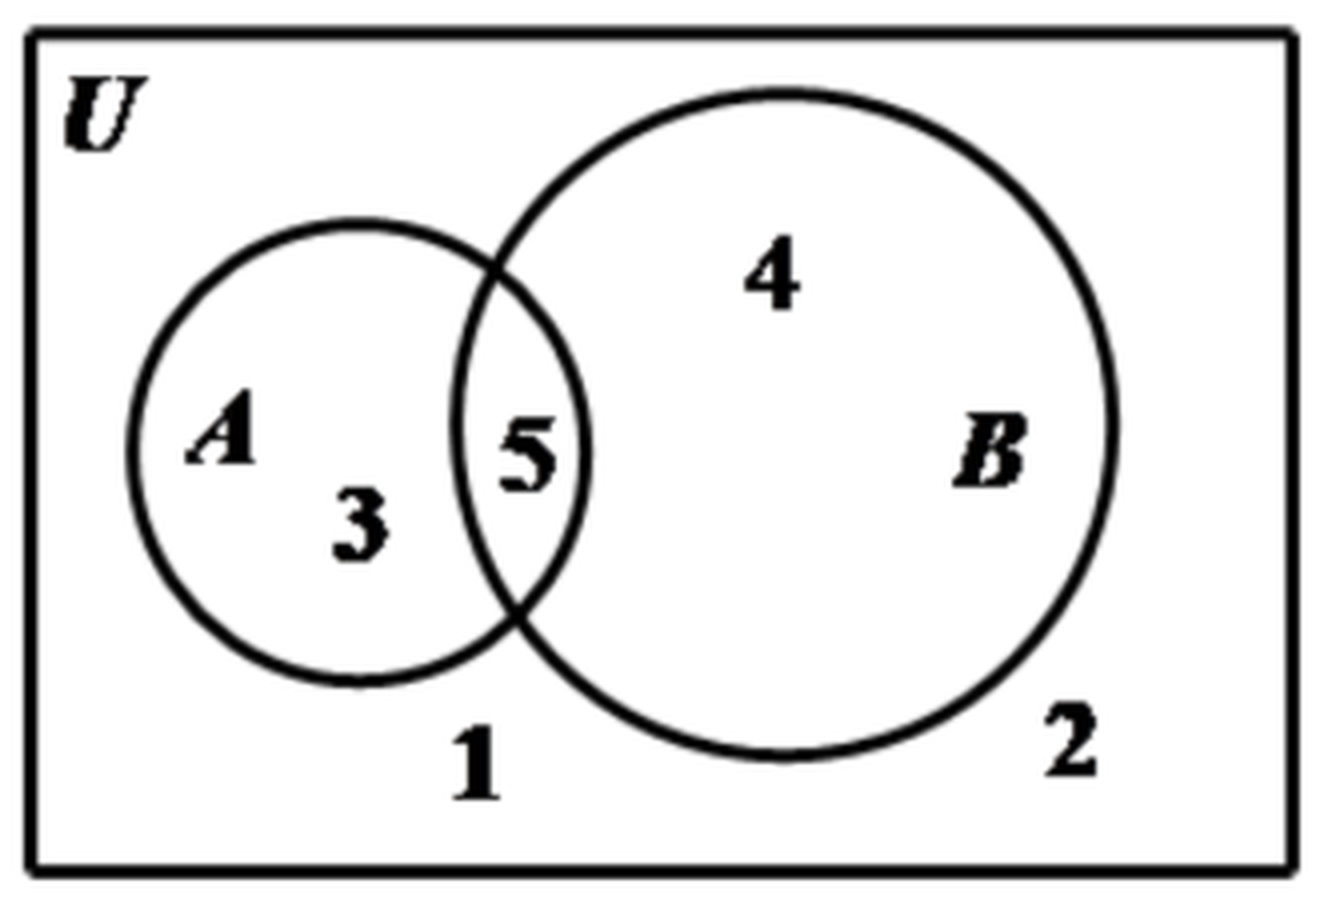
\includegraphics[width=0.28\textwidth]{figures/venn_U5_AB.png}
\end{center}

\keepwithprev
A. $3\notin A$ 且 $3\notin B$\qquad\qquad B. $3\in A$ 且 $3\in B$

C. $3\notin A$ 且 $3\in B$\qquad\qquad D. $3\in A$ 且 $3\notin B$

\ans{$D$}

\ifanswer
\solbegin
\step{画出韦恩图，得 $A=\{5,3\}$，$B=\{5,4\}$，}
\step{则 $3\in A$ 且 $3\notin B$. 故选 $D$.}
\solend

\fi

% 同第 13 题：整块（题干 + 图 + 选项）在答案版还要再挂【答案】【解析】，页末更易被拆开。
\needvspace{7.5cm}
\item 如图表示图形阴影部分的是\mbox{（\quad）}

\begin{center}
% 图取原卷截图、4× LANCZOS 放大（三圆 $A$、$B$、$C$，阴影为整个 $A$ 圆加 $B\cap C$）。
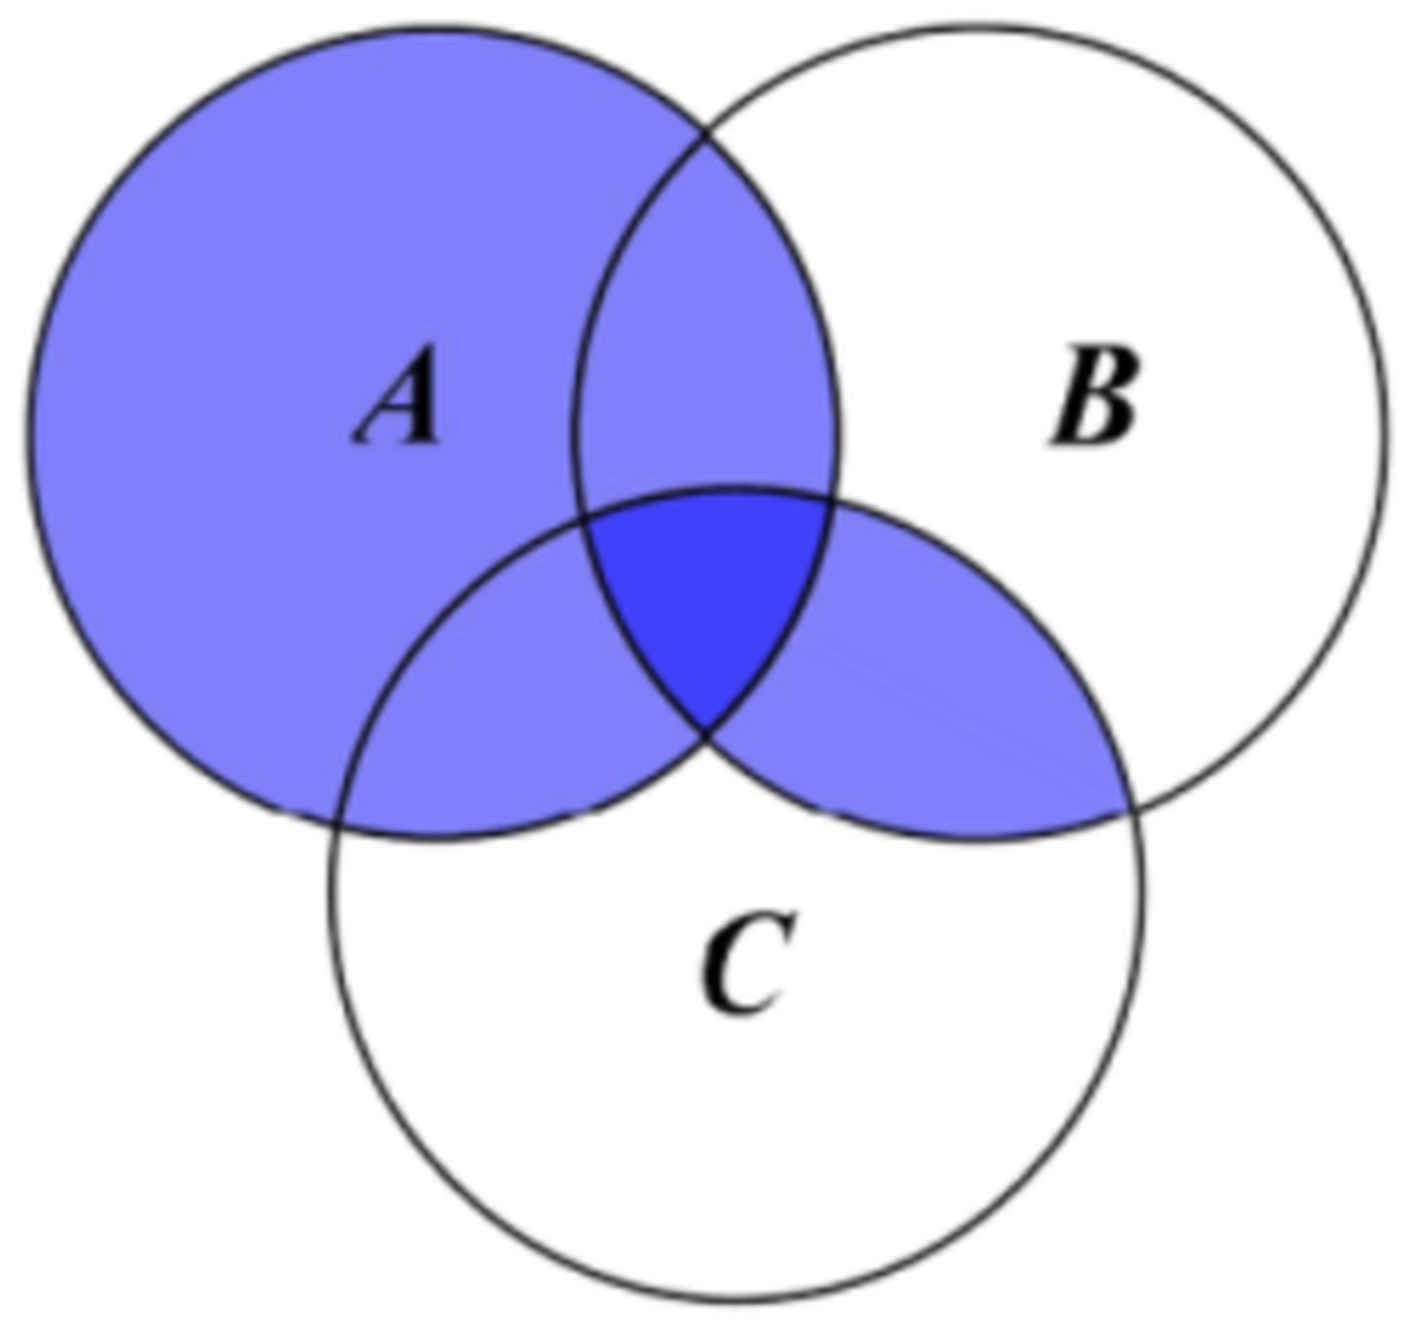
\includegraphics[width=0.30\textwidth]{figures/venn_A_union_BC.png}
\end{center}

\keepwithprev
A. $(A\cup C)\cap(B\cup C)$\qquad\qquad B. $(A\cup B)\cap(A\cup C)$

C. $(A\cup B)\cap(B\cup C)$\qquad\qquad D. $(A\cup B)\cap C$

\ans{$B$}

\ifanswer
\solbegin
\step{图中阴影部分表示元素满足是 $A$ 中的元素，或者是 $B$ 与 $C$ 的公共元素，}
\step{故可以表示为 $A\cup(B\cap C)$，也可以表示为 $(A\cup B)\cap(A\cup C)$.
故选 $B$.}
\solend

\fi

\item 设集合 $M=\left\{x\mid m\leqslant x\leqslant m+\dfrac34\right\}$，
$N=\left\{x\mid n-\dfrac13\leqslant x\leqslant n\right\}$，且 $M$、$N$ 都是集合
$\{x\mid0\leqslant x\leqslant1\}$ 的子集，如果把 $b-a$ 叫做集合
$\{x\mid a\leqslant x\leqslant b\}$ 的“长度”，那么集合 $M\cap N$ 的“长度”的
最小值是\mbox{（\quad）}

\keepwithprev
A. $\dfrac23$\qquad B. $\dfrac1{12}$\qquad C. $\dfrac13$\qquad D. $\dfrac5{12}$

\ans{$B$}

\ifanswer
\solbegin
\step{$M$ 的长度为 $\dfrac34$，$N$ 的长度为 $\dfrac13$，}
\step{当集合 $M\cap N$ 的长度的最小值时，$M$ 与 $N$ 应分别在区间 $[0,1]$ 的左右两端，}
\step{故 $M\cap N$ 的长度的最小值是 $\dfrac34+\dfrac13-1=\dfrac1{12}$，故选 $B$.}
\solend

\fi

\item 定义集合运算 $A-B=\{x\mid x\in A\text{ 且 }x\notin B\}$ 称为集合 $A$ 与集合 $B$ 的
差集；定义集合运算 $A\Delta B=(A-B)\cup(B-A)$ 称为集合 $A$ 与集合 $B$ 的对称差，
有以下 $4$ 个等式：① $A\Delta B=B\Delta A$；② $(A\Delta B)\Delta C=A\Delta(B\Delta C)$；
③ $A\cap(B\Delta C)=(A\cap B)\Delta(A\cap C)$；
④ $A\cup(B\Delta C)=(A\cup B)\Delta(A\cup C)$，
则 $4$ 个等式中恒成立的是\mbox{（\quad）}

\keepwithprev
A. ①②\qquad B. ①②③\qquad C. ①②④\qquad D. ①②③④

\ans{$B$}

\ifanswer
\solbegin
\step{对于①，由 $B\Delta A=(B-A)\cup(A-B)=(A-B)\cup(B-A)=A\Delta B$，
所以①正确；}
\step{对于②，由 $A-B=\{x\mid x\in A\text{ 且 }x\notin B\}
=\{x\mid x\in A,x\notin(A\cap B)\}=A-(A\cap B)$，}
\step{同理可得 $B-A=B-(A\cap B)$，}
\step{则 $A\Delta B=(A-B)\cup(B-A)=(A\cup B)-(A\cap B)$，}
\step{所以 $(A\Delta B)\Delta C=(A\Delta B)\cup C-(A\Delta B)\cap C$，}
\step{所以表示的集合为图（1）中阴影部分所表示的集合，如图所示，}
\step{同理 $A\Delta(B\Delta C)=A\cup(B\Delta C)-A\cap(B\Delta C)$，
也表示图（1）中阴影部分所表示的集合，}
\step{所以 $(A\Delta B)\Delta C=A\Delta(B\Delta C)$，所以②正确；}

\begin{center}
% 图取原卷截图、4× LANCZOS 放大（原卷印在下一页顶部，共三幅三圆韦恩图：
% 图（1）一幅、图（2）左右两幅，图（2）两幅下方各有一行式子标注）。
% 图只在【解析】里出现，故放进 \ifanswer 块，试卷版不排。
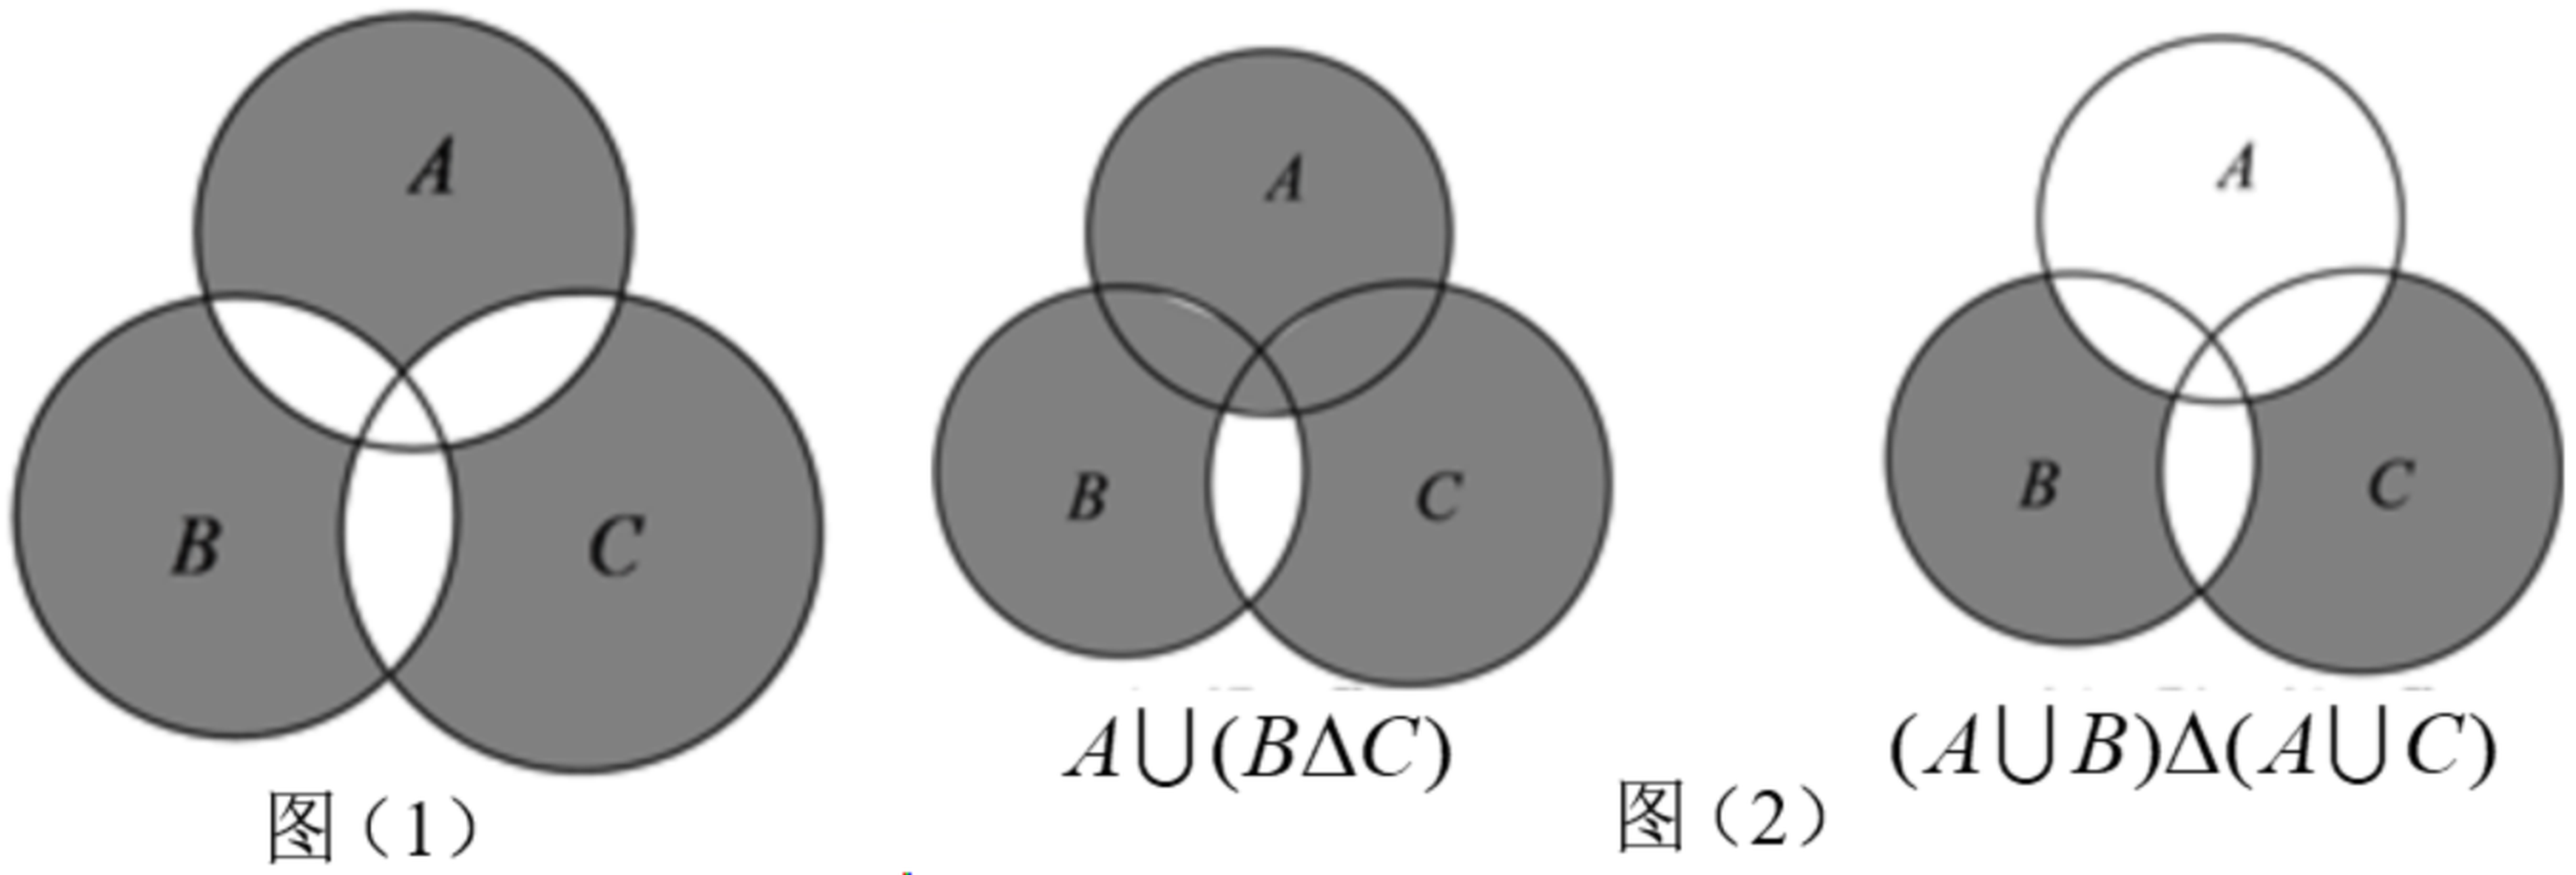
\includegraphics[width=0.86\textwidth]{figures/venn_symdiff3.png}
\end{center}

\step{对于③，由 $A\cap(B\Delta C)=A\cap(B\cup C-B\cap C)
=A\cap(B\cup C)-A\cap(B\cap C)$}
\step{$=(A\cap B)\cup(A\cap C)-(A\cap B)\cap(A\cap C)=(A\cap B)\Delta(A\cap C)$，
所以③正确；}
\step{对于④，如图（2）所示，$A\cup(B\Delta C)\neq(A\cup B)\Delta(A\cup C)$，
所以④错误.}
\step{故选 $B$.}
\solend

\fi

\end{enumerate}

\bigsec{三、解答题}

\begin{enumerate}
\setcounter{enumi}{16}

\item 已知集合 $M=\{x\mid a-1\leqslant x\leqslant2a+3\}$，$P=\{x\mid-2<x\leqslant4\}$，
全集 $U=\R$.

\begin{enumerate}[label=(\arabic*)]
\item 当 $a=2$ 时，求 $M\cap P$；
\item 若 $x\in P$ 是 $x\in M$ 的必要不充分条件，求实数 $a$ 的取值范围.
\end{enumerate}

\ifanswer
\solbegin
\stepm{(1)}{当 $a=2$ 时，集合 $M=\{x\mid1\leqslant x\leqslant7\}$，}
\step{所以 $M\cap P=\{x\mid1\leqslant x\leqslant4\}$；}
\stepm{(2)}{因为 $x\in P$ 是 $x\in M$ 的必要不充分条件，所以 $M\subset P$，}
\step{当 $M=\varnothing$ 时，$a-1>2a+3$，解得 $a<-4$，}
\step{当 $M\neq\varnothing$ 时，则
$\begin{cases}a-1\leqslant2a+3\\ a-1>-2\\ 2a+3\leqslant4\end{cases}$，
解得 $-1<a\leqslant\dfrac12$，}
\step{综上所述，实数 $a$ 的取值范围为
$(-\infty,-4)\cup\left(-1,\dfrac12\right]$.}
\solend

\fi

\ansspace[6]

\item 一辆汽车在某段路程中的行驶速度与时间的关系如图：

\begin{center}
% 图取原卷截图、4× LANCZOS 放大（速度—时间图：纵轴 $v/(\mathrm{km/h})$、
% 横轴 $t(\mathrm{h})$，$t\in[0,1]$、$[1,2]$、$[2,3]$ 三段矩形条高 50、80、90）。
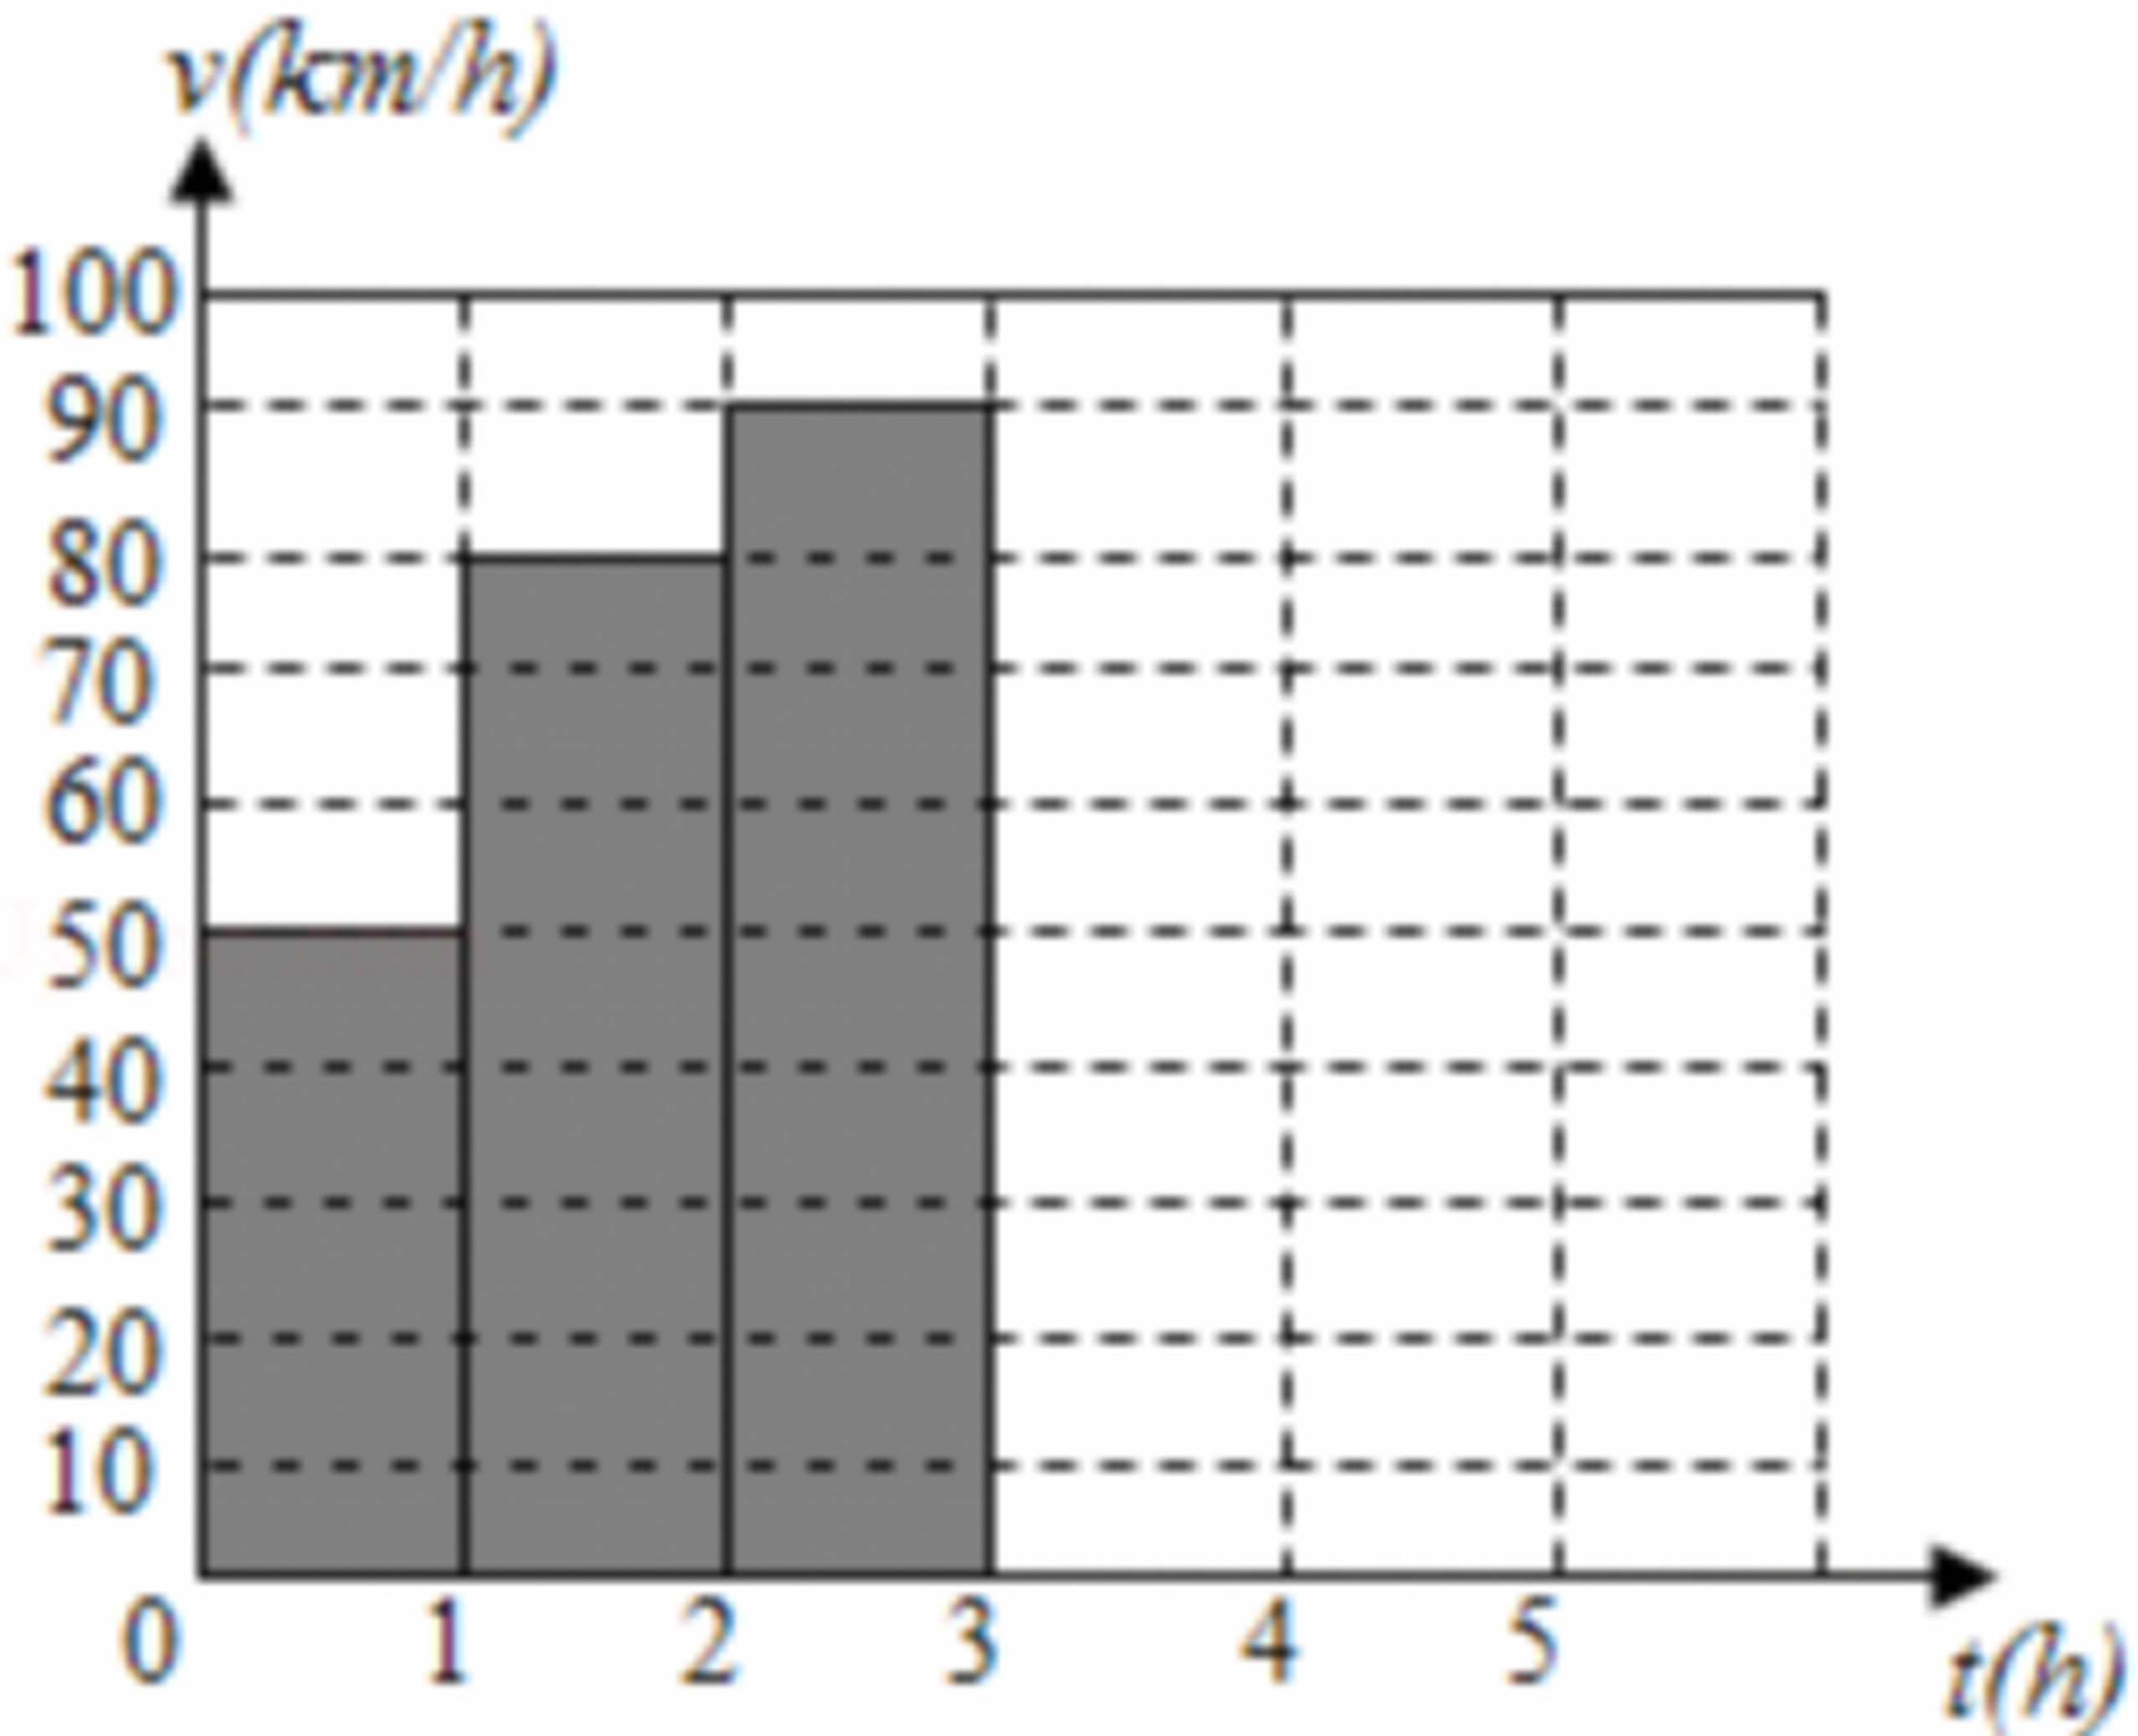
\includegraphics[width=0.52\textwidth]{figures/speed_time_bars.png}
\end{center}

\begin{enumerate}[label=(\arabic*)]
\item 求图中阴影部分的面积，并说明所求面积的实际意义；
\item 假设这辆汽车的里程表在汽车行驶这段路程前的读数为 $2004\,\mathrm{km}$，
试将汽车行驶这段路程时汽车里程表读数 $S$ 表示为时间 $t$ 的函数，
并求出当汽车里程表读数为 $2094\,\mathrm{km}$ 时，汽车行驶了多少时间？
\end{enumerate}

\ifanswer
\solbegin
\stepm{(1)}{由一辆汽车在某段路程中的行驶速度与时间的关系图，}
\step{得阴影部分的面积为 $50\times1+80\times1+90\times1=220$，}
\step{阴影部分的面积表示汽车在 $3$ 小时内行驶的路程为 $220\,\mathrm{km}$.}
\stepm{(2)}{$S=\begin{cases}
50t+2004,&0\leqslant t<1\\
80(t-1)+2054,&1\leqslant t<2\\
90(t-2)+2134,&2\leqslant t\leqslant3
\end{cases}$}
\step{令 $80(t-1)+2054=2094$，解得 $t=1.5$，所以汽车行驶 $1.5$ 小时.}
\solend

\fi

\ansspace[6]

\item 已知集合 $A=\{x\mid x<-2\text{ 或 }x\geqslant3\}$，$U=\R$.

\begin{enumerate}[label=(\arabic*)]
\item 求 $\overline{A}$；
\item 若 $B=\{x\mid mx-1>0\}$，当 $B\sub A$ 时，求实数 $m$ 的取值范围；
\item 若 $B=\{x\mid2m-6\leqslant x\leqslant m+4\}$，当 $B\cap\overline{A}=\varnothing$ 时，
求实数 $m$ 的取值范围.
\end{enumerate}

\ifanswer
\solbegin
\stepm{(1)}{因为集合 $A=\{x\mid x<-2\text{ 或 }x\geqslant3\}$，$U=\R$，
所以 $\overline{A}=\{x\mid-2\leqslant x<3\}$；}
\stepm{(2)}{当 $m=0$ 时，$B=\varnothing$，符合题意，}
\step{当 $m>0$ 时，$B=\left\{x\mid x>\dfrac1m\right\}$，则 $\dfrac1m\geqslant3$，
解得 $0<m\leqslant\dfrac13$，}
\step{当 $m<0$ 时，$B=\left\{x\mid x<\dfrac1m\right\}$，则 $\dfrac1m\leqslant-2$，
解得 $-\dfrac12\leqslant m<0$，}
\step{综上所述，实数 $m$ 的取值范围 $\left[-\dfrac12,\dfrac13\right]$；}
\stepm{(3)}{由题意得 $B=\{x\mid2m-6\leqslant x\leqslant m+4\}$，
$\overline{A}=\{x\mid-2\leqslant x<3\}$，且 $B\cap\overline{A}=\varnothing$，}
\step{当 $B=\varnothing$ 时，$2m-6>m+4$，解得 $m>10$，}
\step{当 $B\neq\varnothing$ 时，则 $\begin{cases}2m-6\leqslant m+4\\ m+4<-2\end{cases}$
或 $\begin{cases}2m-6\leqslant m+4\\ 2m-6\geqslant3\end{cases}$，}
\step{解得 $m<-6$ 或 $\dfrac92\leqslant m\leqslant10$，}
\step{综上所述，实数 $m$ 的取值范围为
$(-\infty,-6)\cup\left[\dfrac92,+\infty\right)$.}
\solend

\fi

\ansspace[8]

\item 在等腰梯形 $ABCD$ 中，$AB=DC=5$，$AD=4$，$BC=10$. 点 $E$ 在下底边 $BC$ 上.
点 $F$ 在腰 $AB$ 上.

\begin{center}
% 图取原卷截图、4× LANCZOS 放大（等腰梯形 $ABCD$ 与线段 $FE$，无辅助线）。
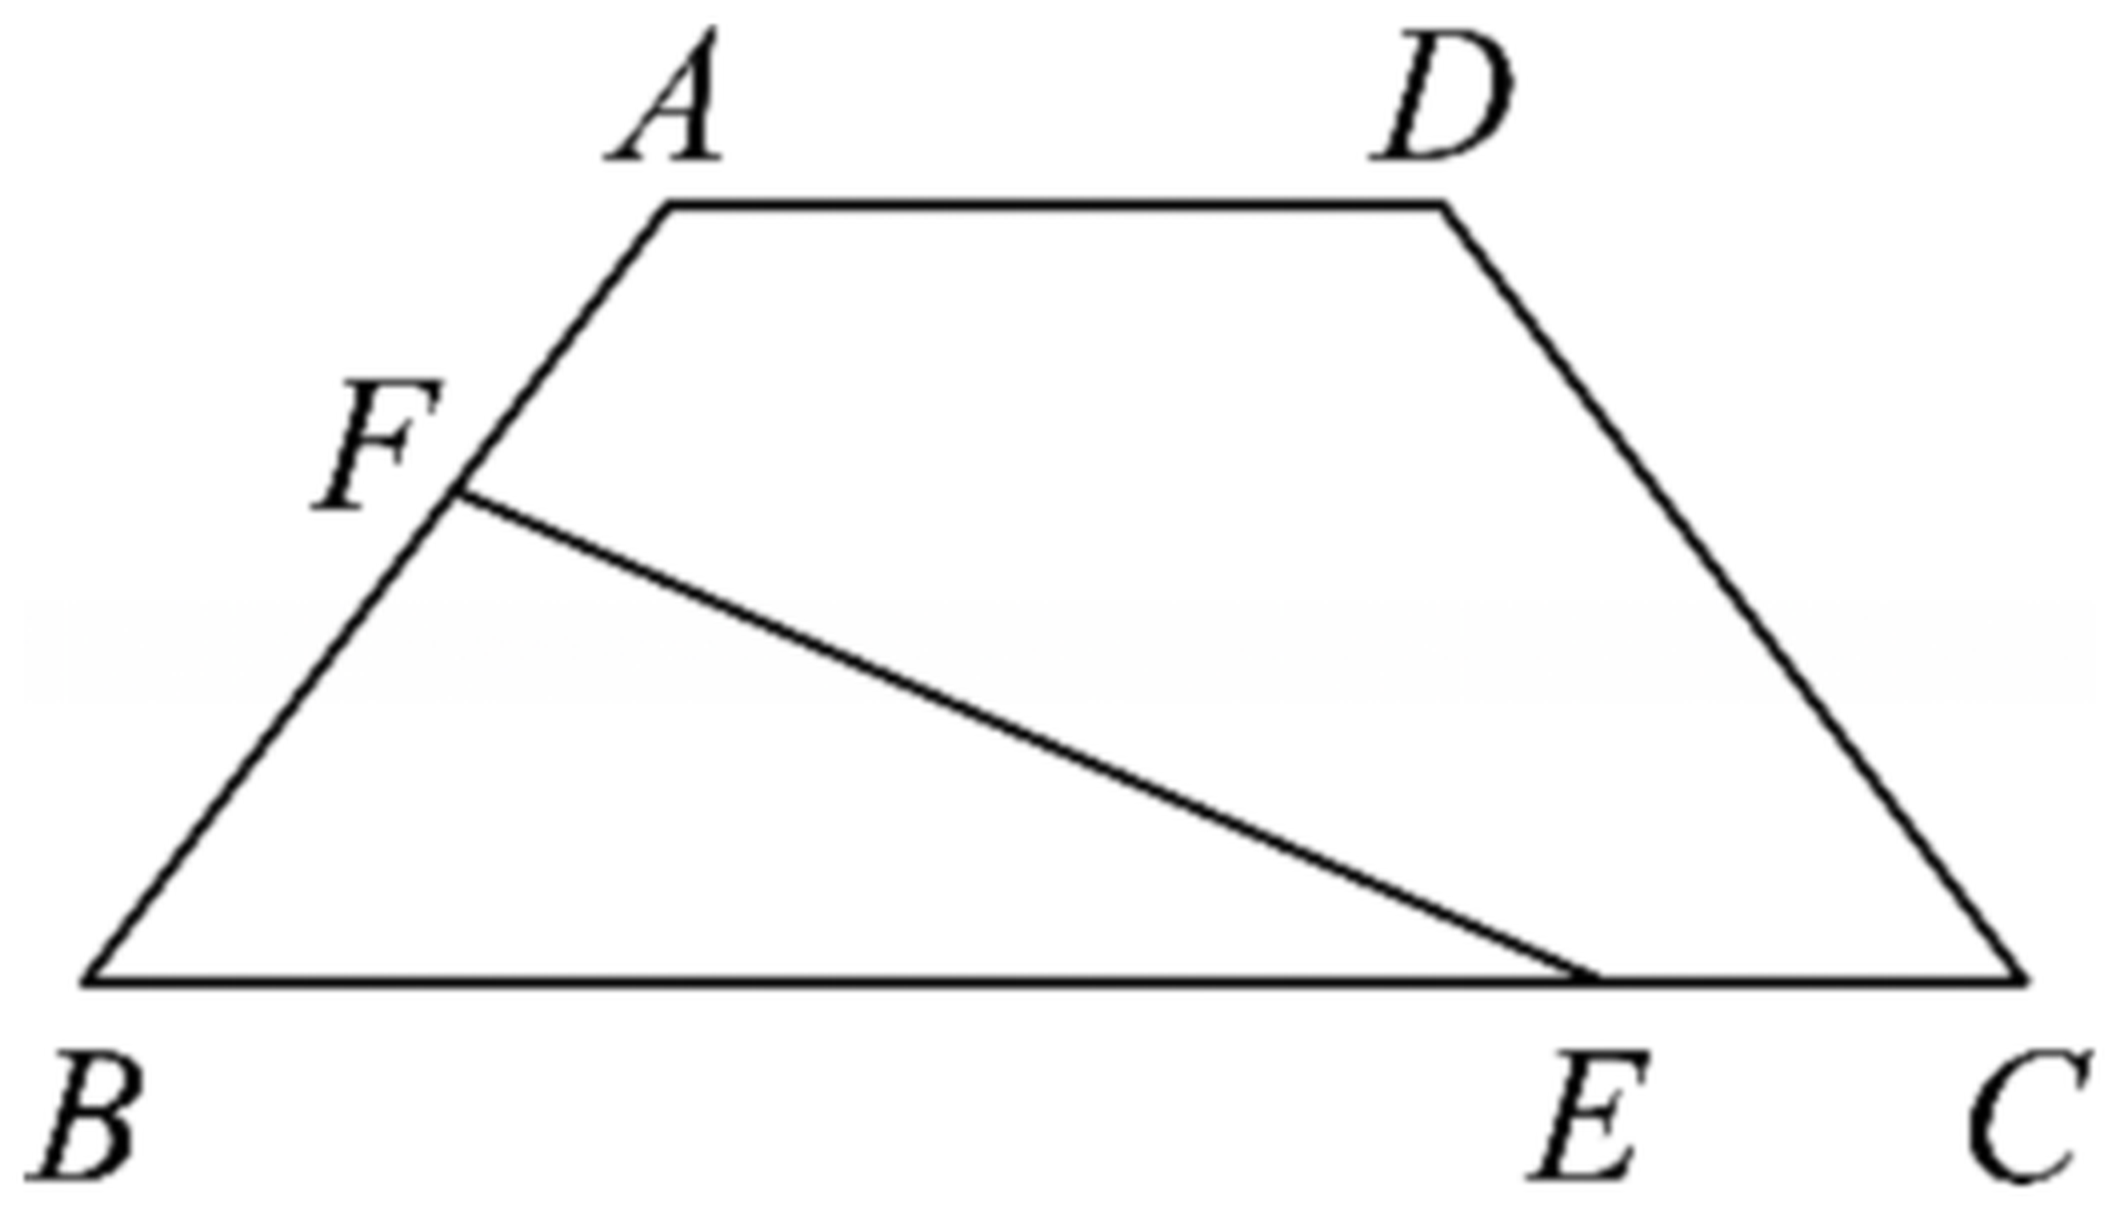
\includegraphics[width=0.46\textwidth]{figures/trapezoid_EF.png}
\end{center}

\begin{enumerate}[label=(\arabic*)]
\item 若 $EF$ 平分等腰梯形 $ABCD$ 的周长，设 $BE$ 长为 $x$，试用含 $x$ 的代数式表示
$\triangle BEF$ 的面积；
\item 是否存在线段 $EF$ 将等腰梯形 $ABCD$ 的周长和面积同时平分？若存在，求出此时 $BE$
的长；若不存在，请说明理由；
\item 是否存在线段 $EF$ 将等腰梯形 $ABCD$ 的周长和面积同时分成 $1:2$ 的两部分？
若存在，求此时 $BE$ 的长；若不存在，请说明理由.
\end{enumerate}

\ifanswer
\solbegin
\stepm{(1)}{过 $A$ 作 $AK\perp BC$ 交 $BC$ 于点 $K$，过 $F$ 作 $FG\perp BC$ 交 $BC$ 于点
$G$，}

\begin{center}
% 图取原卷截图、4× LANCZOS 放大（同梯形，多出虚线 $FG\perp BC$ 与 $AK\perp BC$
% 及两处直角符号；图只在【解析】里出现，故放进 \ifanswer 块）。
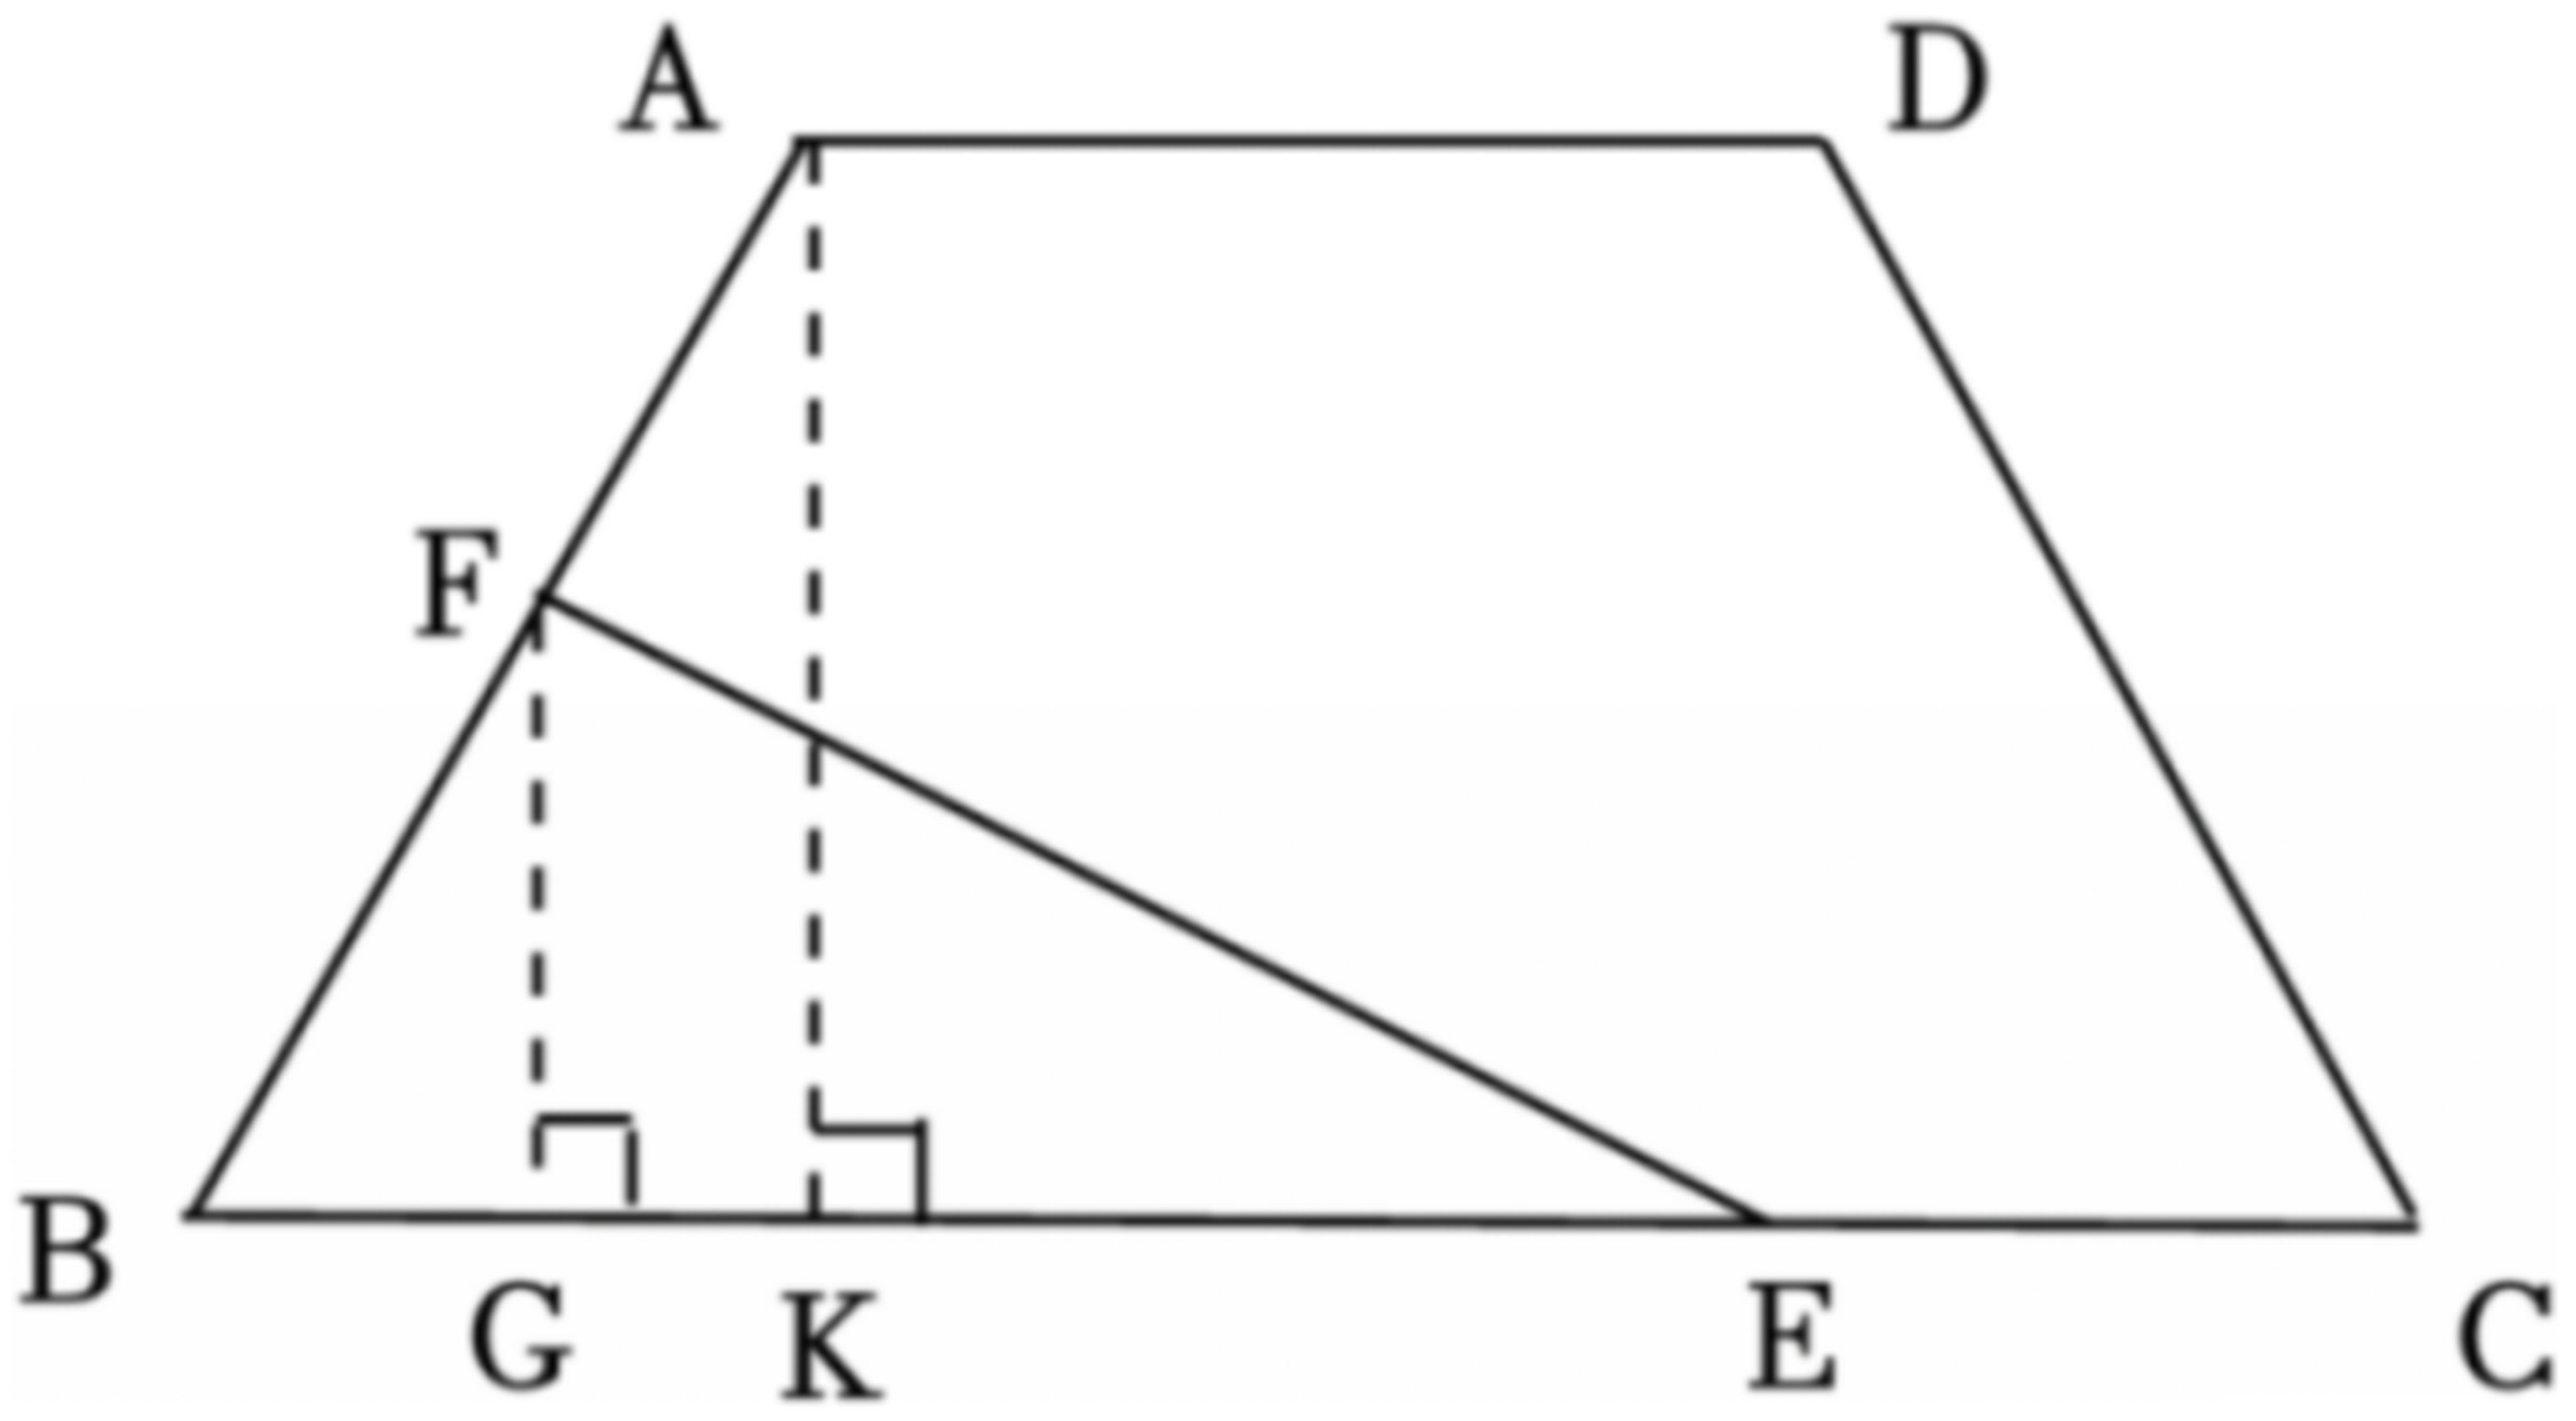
\includegraphics[width=0.62\textwidth]{figures/trapezoid_EF_aux.png}
\end{center}

\step{所以 $BK=\dfrac12\times(BC-AD)=\dfrac12\times(10-4)=3$，}
\step{$AK=\sqrt{AB^2-BK^2}=\sqrt{5^2-3^2}=4$，}
\step{由题意得，梯形 $ABCD$ 周长为 $24$，高为 $4$，面积为 $28$，}
\step{因为 $EF$ 平分等腰梯形 $ABCD$ 的周长，设 $BE$ 长为 $x$，则 $BF=12-x$，}
\step{由 $\begin{cases}0\leqslant12-x\leqslant5\\ 0\leqslant x\leqslant10\end{cases}$，
解得 $7\leqslant x\leqslant10$，}
\step{由题意得 $\triangle BFG\backsim\triangle BAK$，所以 $\dfrac{FG}{AK}=\dfrac{BF}{BA}$，
即 $\dfrac{FG}4=\dfrac{12-x}5$，}
\step{解得 $FG=\dfrac45(12-x)$，}
\step{所以 $S_{\triangle BEF}=\dfrac12BE\cdot FG
=-\dfrac25x^2+\dfrac{24}5x$（$7\leqslant x\leqslant10$）；}
\stepm{(2)}{存在，由 (1) 得 $-\dfrac25x^2+\dfrac{24}5x=\dfrac{28}2$，$x\in[7,10]$，}
\step{即 $x^2-12x+35=0$，解得 $x=7$ 或 $x=5$（舍去），}
\step{所以存在线段 $EF$ 将等腰梯形 $ABCD$ 的周长和面积同时平分，此时 $BE=7$；}
\stepm{(3)}{不存在，}
\step{情况一：$\triangle BEF$ 的面积$:$多边形 $AFECD$ 的面积 $=1:2$，
$(BE+BF):(AF+AD+DC+CE)=1:2$，}
\step{梯形周长的 $\dfrac13$ 是 $\dfrac{24}3=8$，面积的 $\dfrac13$ 是 $\dfrac{28}3$，}
\step{又因为 $BE=x$，所以 $BF=8-x$，}
\step{又因为 $\dfrac{FG}{AK}=\dfrac{BF}{BA}$，即 $\dfrac{FG}4=\dfrac{8-x}5$，
所以 $FG=\dfrac{32-4x}5$，}
\step{所以 $S_{\triangle BEF}=\dfrac12BE\times FG=-\dfrac25x^2+\dfrac{16}5x$，
所以 $\dfrac{28}3=-\dfrac25x^2+\dfrac{16}5x$，}
\step{整理得 $-3x^2+24x-70=0$，此时 $\Delta<0$，无解，故不存在；}
\step{情况二：$\triangle BEF$ 的面积$:$多边形 $AFECD$ 的面积 $=2:1$，
$(BE+BF):(AF+AD+DC+CE)=2:1$，}
\step{梯形周长的 $\dfrac13$ 为 $\dfrac{24}3=8$，面积的 $\dfrac13$ 为 $\dfrac{28}3$，
又 $BE=x$，所以 $BF=16-x$，}
\step{又 $\dfrac{FG}{AK}=\dfrac{BF}{BA}$，即 $\dfrac{FG}4=\dfrac{16-x}5$，
所以 $FG=\dfrac{64-4x}5$，}
\step{所以 $S_{\triangle BEF}=\dfrac12BE\times FG=-\dfrac25x^2+\dfrac{32}5x$，}
\step{所以 $\dfrac{28}3\times2=-\dfrac25x^2+\dfrac{32}5x$，
整理得 $-3x^2+48x-140=0$，}
\step{解得 $x=\dfrac{48+\sqrt{624}}6>10$，$x=\dfrac{48-\sqrt{624}}6<7$，
不符合题意，舍去，故不存在；}
\step{综上所述，不存在线段 $EF$ 将等腰梯形 $ABCD$ 的周长和面积同时分成 $1:2$ 的两部分.}
\solend

\fi

\ansspace[8]

\item 对集合 $\{1,2,\cdots,n\}$ 及其每一个非空子集 $A$，定义一个唯一确定的“交替和”
如下：将 $A$ 中的元素按照递减的次序排列，然后将第一个元素交替地减或加后继的元素所得的
结果，例如，子集 $\{1,2,4,6,9\}$ 的“交替和”是 $9-6+4-2+1=6$，子集 $\{5,6\}$ 的
“交替和”是 $6-5=1$，子集 $\{2\}$ 的交替和是 $2$；定义一个唯一确定的“交替积”如下：
将 $A$ 中的元素按照递减的次序排列，然后将第一个元素交替地除以或乘以后继的数所得的结果，
例如，集合 $\{1,2,4,6,9\}$ 的“交替积”是 $9\div6\times4\div2\times1=3$，
$\{5,6\}$ 的“交替积”是 $6\div5=1.2$，$\{2\}$ 的“交替积”是 $2$.

\begin{enumerate}[label=(\arabic*)]
\item 对于 $\{1,2,3,4,5,6,7,8,9\}$，求其所有子集的“交替和”的总和；
\item 对于 $\{1,2,\cdots,n\}$，求其所有子集的“交替和”的总和；
\item 对于 $\left\{n\mid\dfrac{495}{n+2}\in\N,n\in\Z\right\}$ 求其所有子集的
“交替积”的总和.
\end{enumerate}

\ifanswer
\solbegin
\stepm{(1)}{集合 $\{1,2,3,4,5,6,7,8,9\}$ 的子集中，除去 $\{9\}$ 外还有 $2^9-2$ 个
非空子集，}
\step{把这 $2^9-2$ 个非空子集两两组合后分别计算每一组中“交替和”之和，}
\step{组合原则是设 $A_i=\{9,a_1,a_2,\cdots\}$，$A_i^1=\{a_1,a_2,\cdots\}$，}
\step{集合 $A_i^1$ 的元素为集合 $A_i$ 中去掉 $9$ 的所有元素，把 $A_i$ 和 $A_i^1$
结合为一组，}
\step{显然，每组的“交替和”的和为 $9$，共有 $\dfrac{2^9-2}2$ 组，}
\step{所以，所有“交替和”之和应该为 $\dfrac{9(2^9-2)}2+9=2304$；}
\stepm{(2)}{集合 $\{1,2,\cdots,n\}$ 的子集中，除去 $\{n\}$ 外还有 $2^n-2$ 个非空子集，}
\step{把这 $2^n-2$ 个非空子集两两组合后分别计算每一组中“交替和”之和，}
\step{组合原则是设 $A_i=\{n,a_1,a_2,\cdots\}$，$A_i^1=\{a_1,a_2,\cdots\}$，}
\step{集合 $A_i^1$ 的元素为集合 $A_i$ 中去掉 $n$ 的所有元素，把 $A_i$ 和 $A_i^1$
结合为一组，}
\step{显然，每组的“交替和”的和为 $n$，共有 $\dfrac{2^n-2}2$ 组，}
% 注：下一行分子原卷印作花括号（其余同类处皆用圆括号），照抄未改，见文件头“原卷存疑”③。
\step{所以，所有“交替和”之和应该为 $\dfrac{n\{2^n-2\}}2+n=n\cdot2^{n-1}$；}
\stepm{(3)}{集合 $\left\{n\mid\dfrac{495}{n+2}\in\N,n\in\Z\right\}
=\{493,163,97,53,43,31,13,9,7,3,1,-1\}$，}
\step{其中除去 $\{-1\}$ 外还有 $2^{12}-2$ 个非空子集，}
% 注：下一行原卷把“把这”重复印了一次（“把这把这”），照抄未改，见文件头“原卷存疑”②。
\step{把这把这 $2^{12}-2$ 个非空子集两两组合后分别计算每一组中“交替积”之和，}
\step{组合原则是设 $A_j=\{-1,a_1,a_2,\cdots\}$，$A_j^1=\{a_1,a_2,\cdots\}$，}
\step{集合 $A_j^1$ 的元素为集合 $A_j$ 中去掉 $-1$ 的所有元素，把 $A_j$ 和 $A_j^1$
结合为一组，}
\step{显然，每组的“交替积”的和为 $0$，共有 $\dfrac{2^{12}-2}2$ 组，}
\step{所以，所有“交替积”之和应该为 $\dfrac{2^{12}-2}2\times0-1=-1$.}
\solend

\fi

\ansspace*[10]

\end{enumerate}

\end{document}
"
% 紧凑版：xelatex "\def\iscompact{1}% 高一30_南洋模范中学_开学考.tex
%   —— 高一上数学“2026-2027 年南洋模范中学高一上开学考”（试卷版/答案版）
% 试卷版：xelatex 高一30_南洋模范中学_开学考.tex
% 答案版：xelatex "\def\isanswer{1}\input{高一30_南洋模范中学_开学考.tex}"
% 紧凑版：xelatex "\def\iscompact{1}\input{高一30_南洋模范中学_开学考.tex}"
%
% 原始材料是微信公众号图文（公众号“魔都数学加油站”连载“27学年高一 30”，2026-09-23 发布，
% 原文标题“27学年高一30——2026-2027年上海市南洋模范中学高一上开学考”），
% 正文为 11 张 PNG 页。**同一篇里各页分辨率不一致**——第 2、3、9、10 页 4762×6735，
% 其余七页 2560×3620（已逐页打开确认，非下载缺档），取的是 mmbiz.qpic.cn/<hash>/0 的原图档。
% 原文本身就是一份**讲评版**：填空第 3—7 题下方印【答案】，第 8—12 题与其后各题印【解析】。
% 试题文字、答案与解析均照原卷录入，未改内容。卷面的粉色斜水印属水印，未录入。
%
% 卷首标题：原卷印作“2026-2027 年南洋模范中学高一上开学考”（公众号标题里的“上海市”
% 三字卷面标题行没有，本稿照卷面），年份区间按全稿惯例排 en dash，前缀照原卷保留“年”。
%
% 与原卷的排版差异（均已在 README“说明”中交代）：
%   ① 原文自**第 3 题**起（第 1、2 题未在该文中发布），故本稿题号亦自 3 起；
%   ② 原卷本就印有“一、填空题”“二、选择题”“三、解答题”三节标题，本稿照原卷分节，
%      只把标题改排成全稿统一的“大节标题”样式；
%   ③ 原卷填空第 3—7 题只印【答案】行、第 8 题起印【解析】（选择题答案写在解析末句
%      “故选 D／B”里），本稿统一改为试卷版隐去、答案版以 \ans{}／\ifanswer 块给出，
%      两版彻底分离；
%   ④ 子集符号原卷两种并用：第 7 题题干两处、第 19(2) 题作带下划线的 $\subseteq$，
%      第 17(2) 题解析作真包含的 $\subset$，本稿分别照录为 $\sub$ 与 $\subset$；
%   ⑤ 补集符号原卷一律作**上横线**（$\overline{A}$、$\overline{B}$），本稿照录；
%   ⑥ 原卷的实数集 R 一律作斜体（第 4 题、第 17 题与第 19 题题干的 $U=R$），
%      第 21(3) 题的自然数集与整数集作**粗体** $\mathbf{N}$、$\mathbf{Z}$，
%      本稿按全稿惯例统一写作 $\R$、$\N$、$\Z$；
%   ⑦ 原卷填空的横线约两个字宽，本稿按全稿惯例统一排 \blankline[4.4em]；
%   ⑧ 原卷未印副标题，本稿按全稿惯例补出副标题“集合与常用逻辑用语”——但本卷是开学考，
%      范围不止这一章：第 18 题是速度—时间图象题、第 20 题是等腰梯形的周长/面积平分问题，
%      副标题只标了主章节（见文末“高一30 专记”）；
%   ⑨ 第 13、14、18、20 题的图印在题干右侧、第 16 题的三幅图印在【解析】里的下一页顶部、
%      第 20 题【解析】另有一张带辅助线的图，本稿一律移至题干或解析之后；
%      图取原卷截图、4× LANCZOS 放大（见各 \includegraphics 前的注释）。
%
% 原卷存疑三处（均照抄原卷、未改，见源码中该处上方注释）：
%   ① 第 10 题【解析】验证“破晓集”时写的是 $\notin A$、$\in A$（如“$-2-2=-4\notin A$”），
%      但该处讨论的集合原题设里叫 $P$，同题②的“$x+y=2(k_1+k_2)\in A$”亦然——
%      本稿照抄未改（按文意应为 $P$）；
%   ② 第 21 题【解析】(3) 有“把这把这 $2^{12}-2$ 个非空子集”（“把这”重复印了一次）；
%   ③ 同题 (2) 的结论式分子原卷印作花括号 $\dfrac{n\{2^n-2\}}{2}$（其余同类处皆用圆括号）。

\documentclass[a4paper,11pt]{article}
\usepackage{common}

\begin{document}

\examtitlest[3]{2026--2027 年南洋模范中学高一上开学考}{集合与常用逻辑用语}

\bigsec{一、填空题}

\begin{enumerate}
\setcounter{enumi}{2}

\item 若集合 $A=\{x\mid x^2-2kx+7k=0\}$ 有且仅有三个真子集，则 $k$ 的取值范围是
\blankline[4.4em].

\ans{$(-\infty,0)\cup(7,+\infty)$}

\item “存在 $x\in\R$，使得 $x^2+2x+5=0$”的否定形式是 \blankline[4.4em].

\ans{对任何 $x\in\R$，都有 $x^2+2x+5\neq0$}

\item 下列命题中，$p$ 是 $q$ 的必要非充分条件的是 \blankline[4.4em].

① $p:x>2$ 且 $y>3$，$q:x+y>5$；

② $p$：四边形的四个角都相等，$q$：四边形是正方形.

\ans{②}

\item 若“条件 $\alpha:2\leqslant x\leqslant4$”是“条件 $\beta:3m-1\leqslant x\leqslant-m$”的
充分非必要条件，则 $m$ 的取值范围是 \blankline[4.4em].

\ans{$(-\infty,-4]$}

\item 满足 $\{1\}\sub M\sub\{1,2,4,5\}$ 的集合 $M$ 的个数为 \blankline[4.4em] 个.

\ans{$8$}

\item 已知集合 $A=\{1,2\}$，集合 $B=\{x\mid ax=6\}$，若 $A\cup B=A$，则 $a$ 的所有取值
构成的集合为 \blankline[4.4em].

\ifanswer
\solbegin
\step{因为 $A\cup B=A$，所以 $B\sub A$，}
\step{当 $a=0$ 时，$B=\varnothing$，满足 $B\sub A$；}
\step{当 $a\neq0$ 时，$B=\left\{\dfrac6a\right\}$，则 $\dfrac6a=1$ 或 $\dfrac6a=2$，
解得 $a=6$ 或 $a=3$，}
\step{综上所述，$a$ 的所有取值构成的集合为 $\{0,3,6\}$.}
\solend

\fi

\item 对于集合 $M$、$N$，定义 $M-N=\{x\mid x\in M\text{ 且 }x\notin N\}$，
$M\oplus N=(M-N)\cup(N-M)$，设 $A=\{y\mid y=|x|,x\in\R\}$，
$B=\{y\mid y=-(x-1)^2+2,x\in\R\}$，则 $A\oplus B=$ \blankline[4.4em].

\ifanswer
\solbegin
\step{由已知 $A=[0,+\infty)$，$B=(-\infty,2]$，}
\step{由于 $A-B=(2,+\infty)$，$B-A=(-\infty,0)$，}
\step{故 $A\oplus B=(A-B)\cup(B-A)=(-\infty,0)\cup(2,+\infty)$.}
\solend

\fi

\item 设 $P$ 为非空实数集满足：对任意给定的 $x$、$y\in P$（$x$、$y$ 可以相同），都有
$x+y\in P$，$x-y\in P$，$xy\in P$，则称 $P$ 为破晓集. 关于破晓集有下列结论：
①集合 $P=\{-2,-1,0,1,2\}$ 为破晓集；②集合 $P=\{x\mid x=2n,n\in\Z\}$ 为破晓集；
③若集合 $P_1$、$P_2$ 为破晓集，则 $P_1\cup P_2$ 为破晓集；④若集合 $P$ 为破晓集，
则一定有 $0\in P$；⑤若集合 $P_1$、$P_2$ 为破晓集，则 $P_1\cap P_2$ 为破晓集；
其中正确结论的序号是 \blankline[4.4em].

\ifanswer
\solbegin
% 注：以下几步原卷把该集合记作 $A$（题设里叫 $P$），照抄未改，见文件头“原卷存疑”①。
\step{对于①：$-2-2=-4\notin A$，故集合 $P=\{-2,-1,0,1,2\}$ 不为破晓集，故①错误；}
\step{②设 $x$、$y\in A$，则 $x=2k_1$，$y=2k_2$，且 $k_1$、$k_2\in\Z$，}
\step{故 $x+y=2(k_1+k_2)\in A$，$x-y=2(k_1-k_2)\in A$，$xy=4k_1k_2\in A$，}
\step{故集合 $P=\{x\mid x=2n,n\in\Z\}$ 为破晓集，故②正确；}
\step{③若集合 $P_1$、$P_2$ 为破晓集，设 $P_1=\{x\mid x=2k,k\in\Z\}$，
$P_2=\{x\mid x=3k,k\in\Z\}$，}
\step{但是 $P_1\cup P_2$ 不为破晓集，如 $x=2$，$y=3$ 时，$x+y=5$，
故 $5\notin(P_1\cup P_2)$，故③错误；}
\step{④若集合 $P$ 为破晓集，则取 $x=y$，$x-y=0\in A$，则一定有 $0\in P$，故④正确.}
\step{⑤正确；}
\step{故正确的是②④⑤.}
\solend

\fi

\item 已知集合 $M$ 的元素均为正整数，定义集合 $M$ 的“变项和”为：将 $M$ 中每个元素 $m$
都乘以 $(-1)^m$ 后再求和. 若集合 $A=\{n\mid1\leqslant n\leqslant10,n\in\N\}$，则集合 $A$
的所有非空子集的“变项和”的总和为 \blankline[4.4em].

\ifanswer
\solbegin
\step{$A$ 集合的所有非空子集中，每个元素出现的次数都是
$(2^{10}-1)-(2^9-1)=2^9$，}
\step{则集合 $A$ 的所有非空子集的“变项和”的总和为
$1\times(-1)^1\times2^9+2\times(-1)^2\times2^9+\cdots+10\times(-1)^{10}\times2^9$}
\step{$=(-1+2-3+4-\cdots-9+10)\times2^9=5\times2^9=2560$.}
\solend

\fi

\item 已知集合 $A=[t,t+1]\cup[t+4,t+9]$，$0\notin A$，存在正数 $\lambda$，使得对任意
$a\in A$，都有 $\dfrac\lambda a\in A$，则 $t$ 的值是 \blankline[4.4em].

\ifanswer
\solbegin
\step{当 $t>0$ 时，当 $a\in[t,t+1]$ 时，$\dfrac\lambda a\in[t+4,t+9]$，}
\step{当 $a\in[t+4,t+9]$ 时，$\dfrac\lambda a\in[t,t+1]$，}
\step{即当 $a=t$ 时，$\dfrac\lambda a\leqslant t+9$；当 $a=t+9$ 时，
$\dfrac\lambda a\geqslant t$，即 $\lambda=t(t+9)$；}
\step{当 $a=t+1$ 时，$\dfrac\lambda a\geqslant t+4$，当 $a=t+4$ 时，
$\dfrac\lambda a\leqslant t+1$，即 $\lambda=(t+1)(t+4)$，}
\step{所以 $t(t+9)=(t+1)(t+4)$，解得 $t=1$.}
\step{当 $t+1<0<t+4$ 时，当 $a\in[t,t+1]$ 时，$\dfrac\lambda a\in[t,t+1]$.}
\step{当 $a\in[t+4,t+9]$ 时，则 $\dfrac\lambda a\in[t+4,t+9]$，}
\step{即当 $a=t$ 时，$\dfrac\lambda a\leqslant t+1$，当 $a=t+1$ 时，
$\dfrac\lambda a\geqslant t$，即 $\lambda=t(t+1)$，}
\step{即当 $a=t+4$ 时，$\dfrac\lambda a\leqslant t+9$，当 $a=t+9$ 时，
$\dfrac\lambda a\geqslant t+4$，即 $\lambda=(t+4)(t+9)$，}
\step{所以 $t(t+1)=(t+4)(t+9)$，解得 $t=-3$.}
\step{当 $t+9<0$ 时，同理可得无解.}
\step{综上，$t$ 的值为 $1$ 或 $-3$.}
\solend

\fi

\end{enumerate}

\bigsec{二、选择题}

\begin{enumerate}
\setcounter{enumi}{12}

% 这道题是“题干 + 图 + 选项”约 6cm 的一整块，页末放不下就会被拆开（切页审计的 A 类），
% 故在题前先量一次页高：不够就把整道题干连图带选项一起挪到次页。
\needvspace{6.5cm}
\item 设 $U=\{1,2,3,4,5\}$，$A$、$B$ 都是 $U$ 的子集，且 $A\cap B=\{5\}$，
$\overline{A}\cap B=\{4\}$，$\overline{A}\cap\overline{B}=\{1,2\}$，
则以下四个判断中正确的是\mbox{（\quad）}

\begin{center}
% 图取原卷截图、4× LANCZOS 放大（原卷把图印在题干右侧，本稿移至此处，见文件头⑨）。
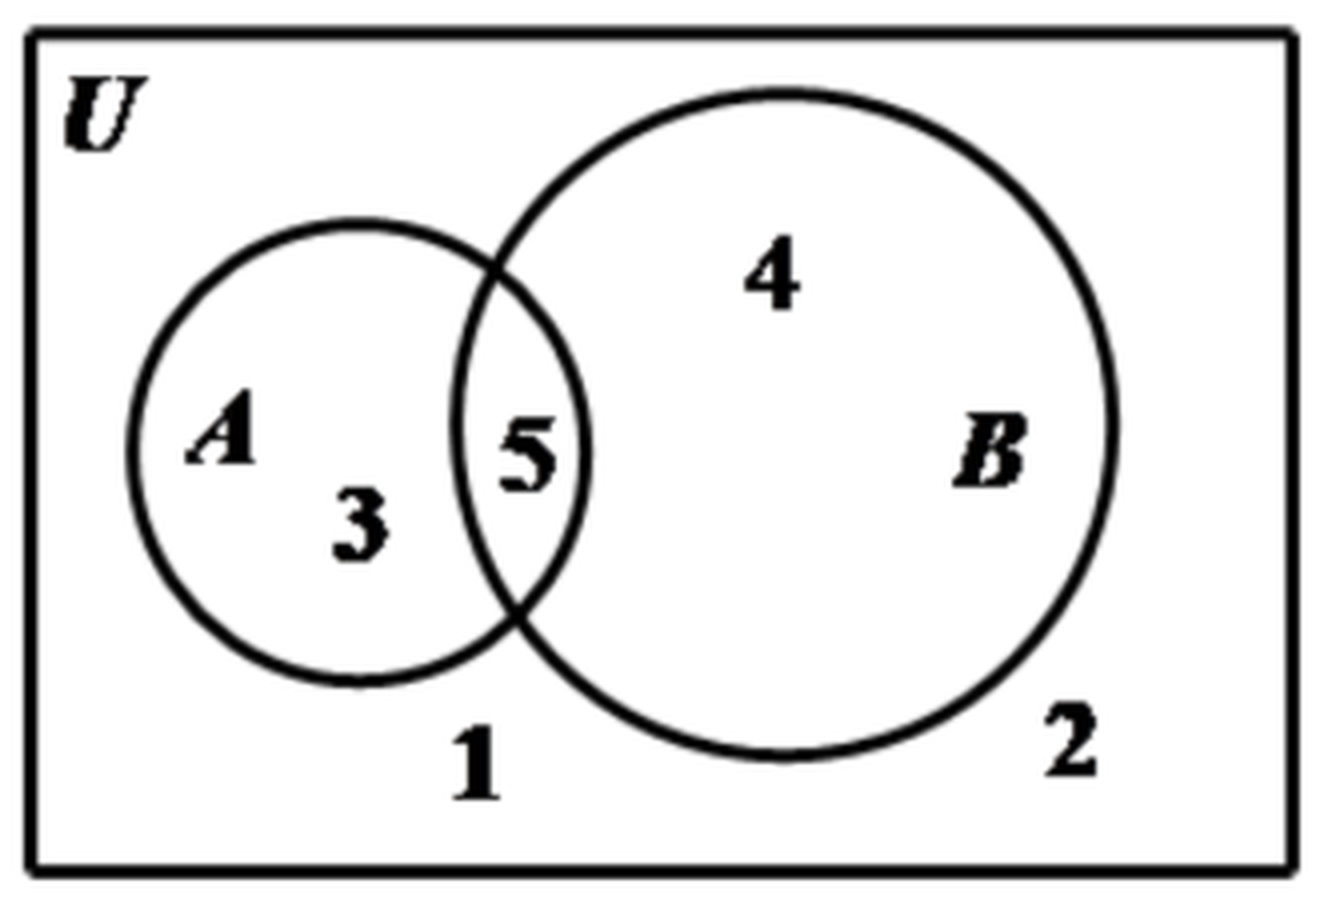
\includegraphics[width=0.28\textwidth]{figures/venn_U5_AB.png}
\end{center}

\keepwithprev
A. $3\notin A$ 且 $3\notin B$\qquad\qquad B. $3\in A$ 且 $3\in B$

C. $3\notin A$ 且 $3\in B$\qquad\qquad D. $3\in A$ 且 $3\notin B$

\ans{$D$}

\ifanswer
\solbegin
\step{画出韦恩图，得 $A=\{5,3\}$，$B=\{5,4\}$，}
\step{则 $3\in A$ 且 $3\notin B$. 故选 $D$.}
\solend

\fi

% 同第 13 题：整块（题干 + 图 + 选项）在答案版还要再挂【答案】【解析】，页末更易被拆开。
\needvspace{7.5cm}
\item 如图表示图形阴影部分的是\mbox{（\quad）}

\begin{center}
% 图取原卷截图、4× LANCZOS 放大（三圆 $A$、$B$、$C$，阴影为整个 $A$ 圆加 $B\cap C$）。
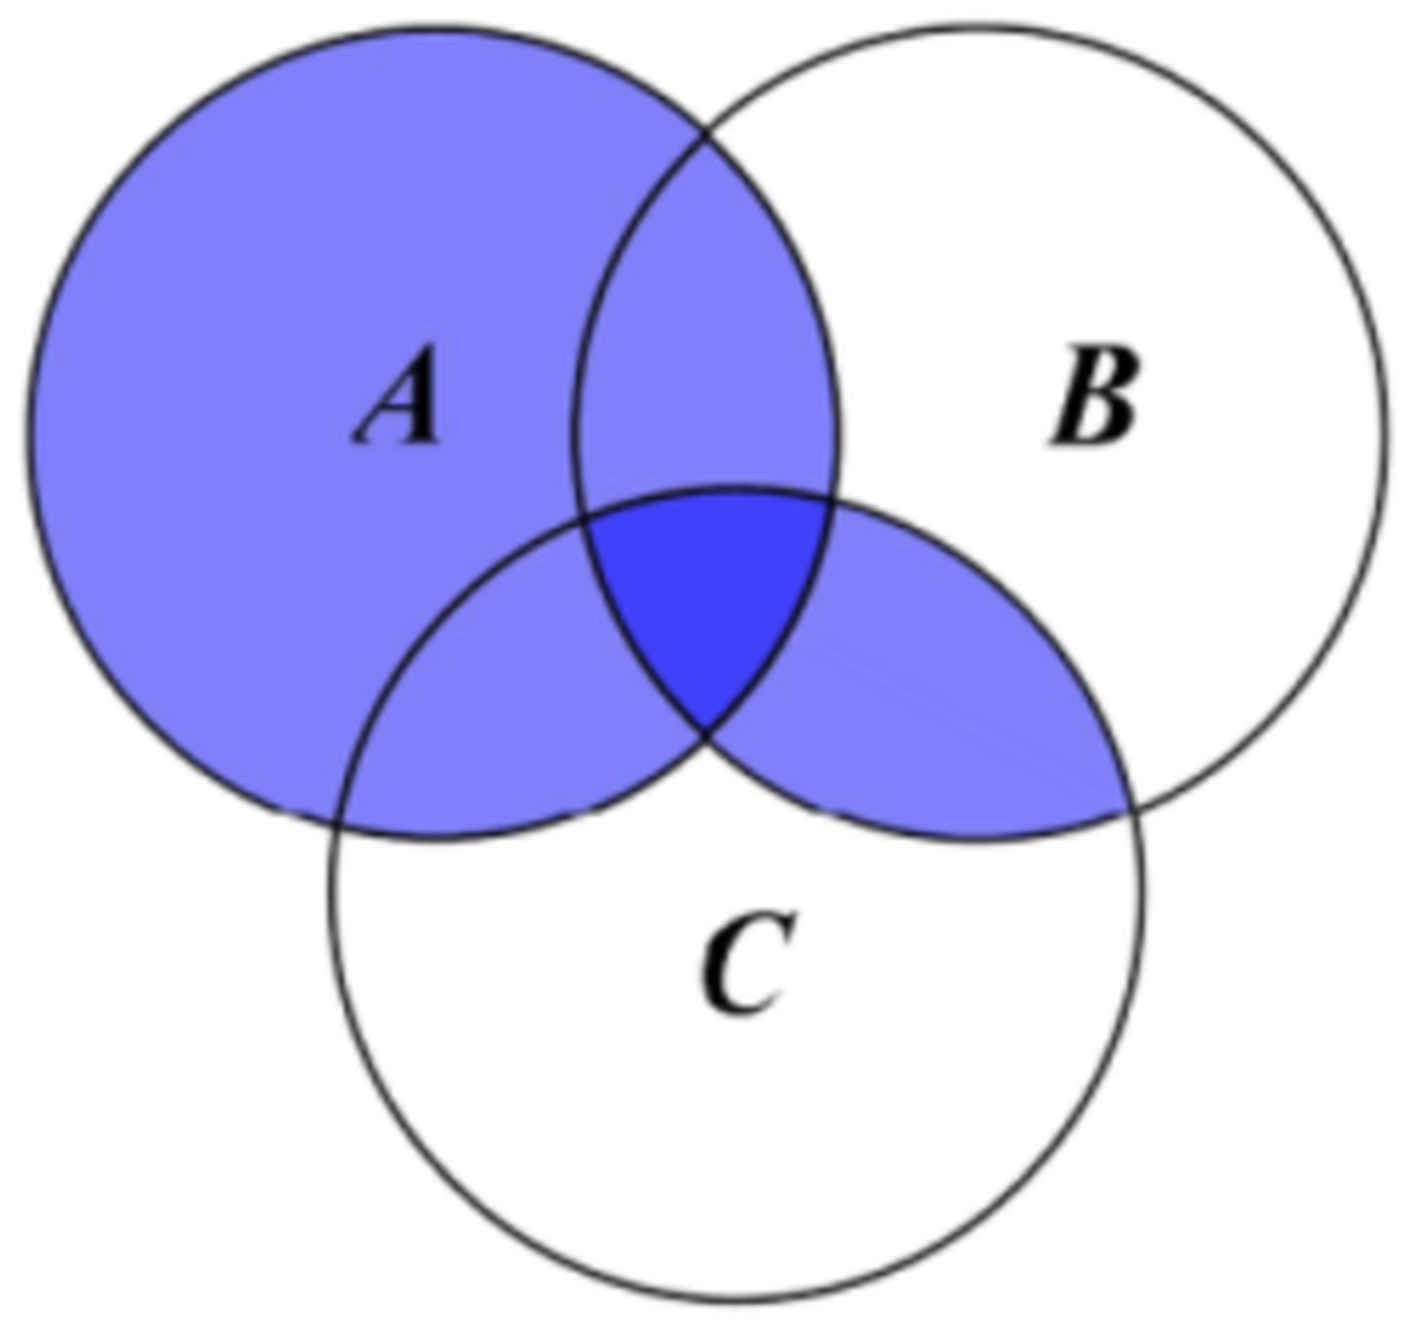
\includegraphics[width=0.30\textwidth]{figures/venn_A_union_BC.png}
\end{center}

\keepwithprev
A. $(A\cup C)\cap(B\cup C)$\qquad\qquad B. $(A\cup B)\cap(A\cup C)$

C. $(A\cup B)\cap(B\cup C)$\qquad\qquad D. $(A\cup B)\cap C$

\ans{$B$}

\ifanswer
\solbegin
\step{图中阴影部分表示元素满足是 $A$ 中的元素，或者是 $B$ 与 $C$ 的公共元素，}
\step{故可以表示为 $A\cup(B\cap C)$，也可以表示为 $(A\cup B)\cap(A\cup C)$.
故选 $B$.}
\solend

\fi

\item 设集合 $M=\left\{x\mid m\leqslant x\leqslant m+\dfrac34\right\}$，
$N=\left\{x\mid n-\dfrac13\leqslant x\leqslant n\right\}$，且 $M$、$N$ 都是集合
$\{x\mid0\leqslant x\leqslant1\}$ 的子集，如果把 $b-a$ 叫做集合
$\{x\mid a\leqslant x\leqslant b\}$ 的“长度”，那么集合 $M\cap N$ 的“长度”的
最小值是\mbox{（\quad）}

\keepwithprev
A. $\dfrac23$\qquad B. $\dfrac1{12}$\qquad C. $\dfrac13$\qquad D. $\dfrac5{12}$

\ans{$B$}

\ifanswer
\solbegin
\step{$M$ 的长度为 $\dfrac34$，$N$ 的长度为 $\dfrac13$，}
\step{当集合 $M\cap N$ 的长度的最小值时，$M$ 与 $N$ 应分别在区间 $[0,1]$ 的左右两端，}
\step{故 $M\cap N$ 的长度的最小值是 $\dfrac34+\dfrac13-1=\dfrac1{12}$，故选 $B$.}
\solend

\fi

\item 定义集合运算 $A-B=\{x\mid x\in A\text{ 且 }x\notin B\}$ 称为集合 $A$ 与集合 $B$ 的
差集；定义集合运算 $A\Delta B=(A-B)\cup(B-A)$ 称为集合 $A$ 与集合 $B$ 的对称差，
有以下 $4$ 个等式：① $A\Delta B=B\Delta A$；② $(A\Delta B)\Delta C=A\Delta(B\Delta C)$；
③ $A\cap(B\Delta C)=(A\cap B)\Delta(A\cap C)$；
④ $A\cup(B\Delta C)=(A\cup B)\Delta(A\cup C)$，
则 $4$ 个等式中恒成立的是\mbox{（\quad）}

\keepwithprev
A. ①②\qquad B. ①②③\qquad C. ①②④\qquad D. ①②③④

\ans{$B$}

\ifanswer
\solbegin
\step{对于①，由 $B\Delta A=(B-A)\cup(A-B)=(A-B)\cup(B-A)=A\Delta B$，
所以①正确；}
\step{对于②，由 $A-B=\{x\mid x\in A\text{ 且 }x\notin B\}
=\{x\mid x\in A,x\notin(A\cap B)\}=A-(A\cap B)$，}
\step{同理可得 $B-A=B-(A\cap B)$，}
\step{则 $A\Delta B=(A-B)\cup(B-A)=(A\cup B)-(A\cap B)$，}
\step{所以 $(A\Delta B)\Delta C=(A\Delta B)\cup C-(A\Delta B)\cap C$，}
\step{所以表示的集合为图（1）中阴影部分所表示的集合，如图所示，}
\step{同理 $A\Delta(B\Delta C)=A\cup(B\Delta C)-A\cap(B\Delta C)$，
也表示图（1）中阴影部分所表示的集合，}
\step{所以 $(A\Delta B)\Delta C=A\Delta(B\Delta C)$，所以②正确；}

\begin{center}
% 图取原卷截图、4× LANCZOS 放大（原卷印在下一页顶部，共三幅三圆韦恩图：
% 图（1）一幅、图（2）左右两幅，图（2）两幅下方各有一行式子标注）。
% 图只在【解析】里出现，故放进 \ifanswer 块，试卷版不排。
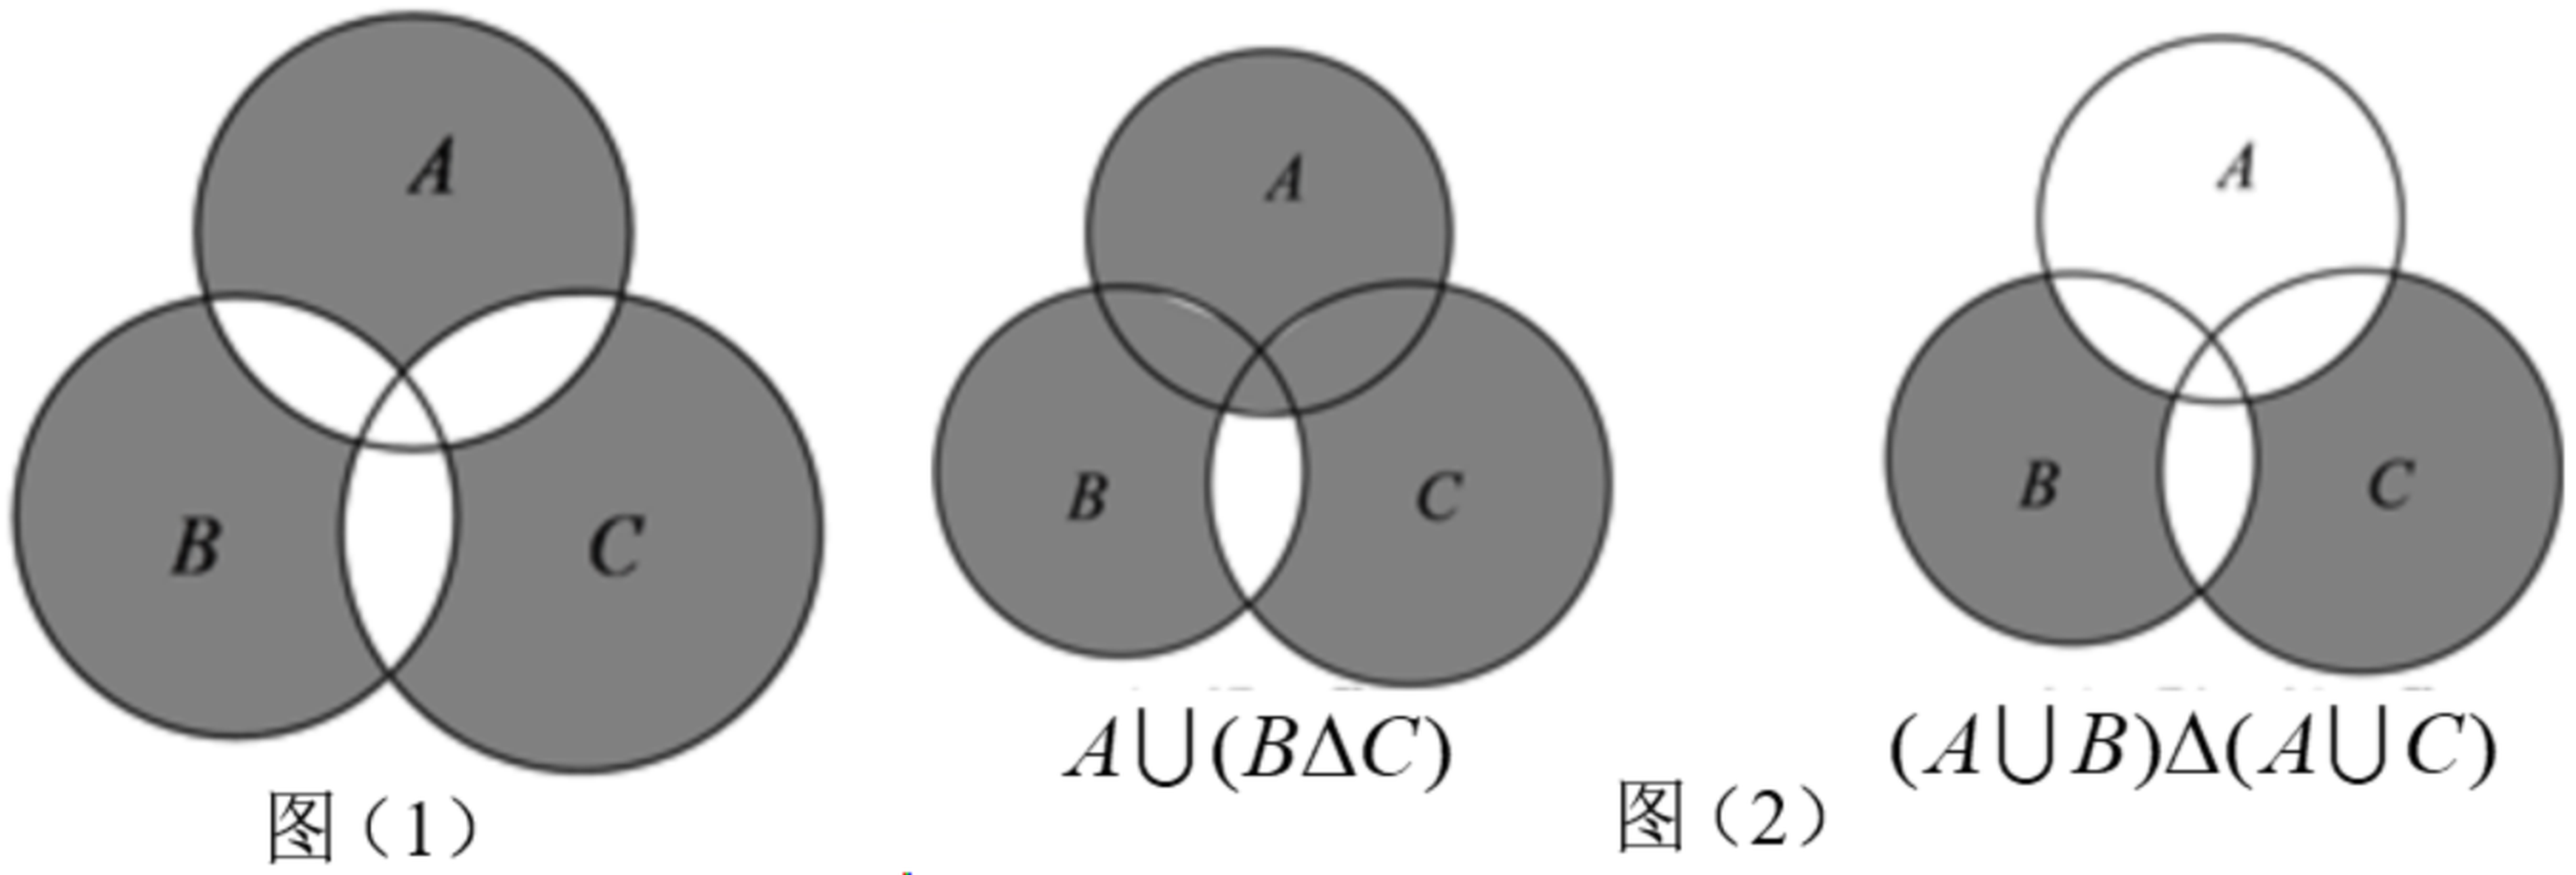
\includegraphics[width=0.86\textwidth]{figures/venn_symdiff3.png}
\end{center}

\step{对于③，由 $A\cap(B\Delta C)=A\cap(B\cup C-B\cap C)
=A\cap(B\cup C)-A\cap(B\cap C)$}
\step{$=(A\cap B)\cup(A\cap C)-(A\cap B)\cap(A\cap C)=(A\cap B)\Delta(A\cap C)$，
所以③正确；}
\step{对于④，如图（2）所示，$A\cup(B\Delta C)\neq(A\cup B)\Delta(A\cup C)$，
所以④错误.}
\step{故选 $B$.}
\solend

\fi

\end{enumerate}

\bigsec{三、解答题}

\begin{enumerate}
\setcounter{enumi}{16}

\item 已知集合 $M=\{x\mid a-1\leqslant x\leqslant2a+3\}$，$P=\{x\mid-2<x\leqslant4\}$，
全集 $U=\R$.

\begin{enumerate}[label=(\arabic*)]
\item 当 $a=2$ 时，求 $M\cap P$；
\item 若 $x\in P$ 是 $x\in M$ 的必要不充分条件，求实数 $a$ 的取值范围.
\end{enumerate}

\ifanswer
\solbegin
\stepm{(1)}{当 $a=2$ 时，集合 $M=\{x\mid1\leqslant x\leqslant7\}$，}
\step{所以 $M\cap P=\{x\mid1\leqslant x\leqslant4\}$；}
\stepm{(2)}{因为 $x\in P$ 是 $x\in M$ 的必要不充分条件，所以 $M\subset P$，}
\step{当 $M=\varnothing$ 时，$a-1>2a+3$，解得 $a<-4$，}
\step{当 $M\neq\varnothing$ 时，则
$\begin{cases}a-1\leqslant2a+3\\ a-1>-2\\ 2a+3\leqslant4\end{cases}$，
解得 $-1<a\leqslant\dfrac12$，}
\step{综上所述，实数 $a$ 的取值范围为
$(-\infty,-4)\cup\left(-1,\dfrac12\right]$.}
\solend

\fi

\ansspace[6]

\item 一辆汽车在某段路程中的行驶速度与时间的关系如图：

\begin{center}
% 图取原卷截图、4× LANCZOS 放大（速度—时间图：纵轴 $v/(\mathrm{km/h})$、
% 横轴 $t(\mathrm{h})$，$t\in[0,1]$、$[1,2]$、$[2,3]$ 三段矩形条高 50、80、90）。
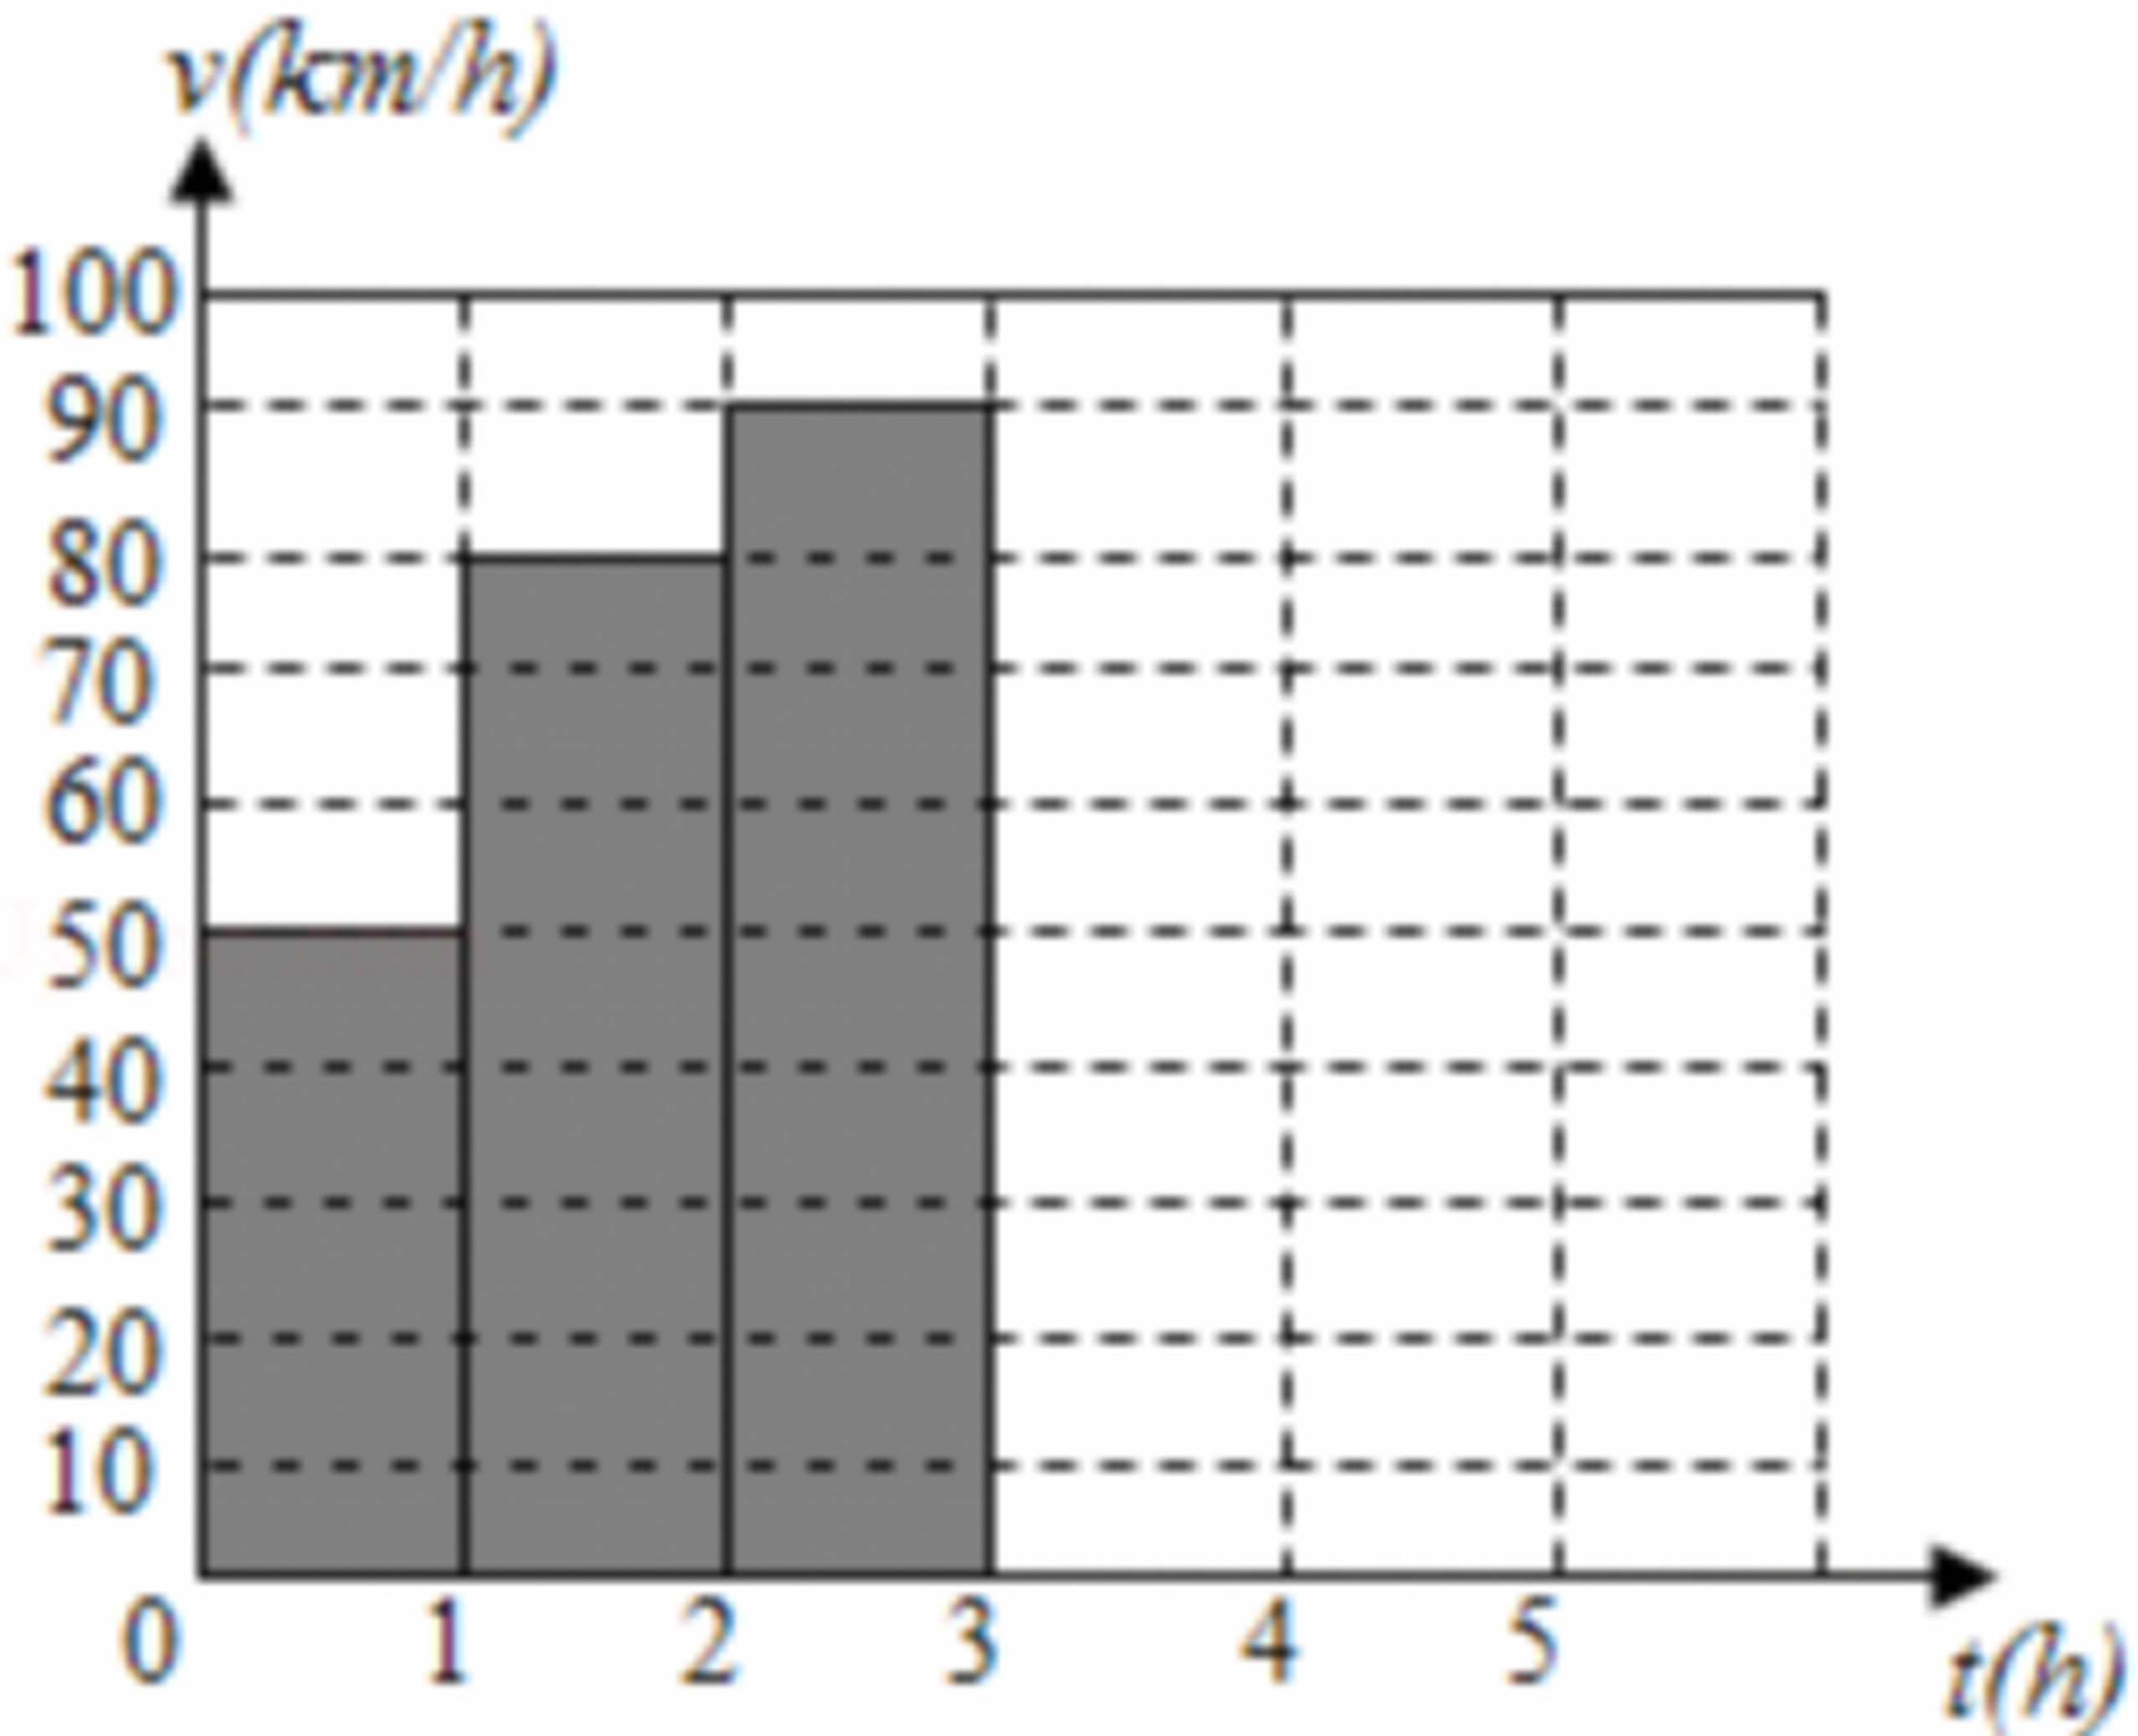
\includegraphics[width=0.52\textwidth]{figures/speed_time_bars.png}
\end{center}

\begin{enumerate}[label=(\arabic*)]
\item 求图中阴影部分的面积，并说明所求面积的实际意义；
\item 假设这辆汽车的里程表在汽车行驶这段路程前的读数为 $2004\,\mathrm{km}$，
试将汽车行驶这段路程时汽车里程表读数 $S$ 表示为时间 $t$ 的函数，
并求出当汽车里程表读数为 $2094\,\mathrm{km}$ 时，汽车行驶了多少时间？
\end{enumerate}

\ifanswer
\solbegin
\stepm{(1)}{由一辆汽车在某段路程中的行驶速度与时间的关系图，}
\step{得阴影部分的面积为 $50\times1+80\times1+90\times1=220$，}
\step{阴影部分的面积表示汽车在 $3$ 小时内行驶的路程为 $220\,\mathrm{km}$.}
\stepm{(2)}{$S=\begin{cases}
50t+2004,&0\leqslant t<1\\
80(t-1)+2054,&1\leqslant t<2\\
90(t-2)+2134,&2\leqslant t\leqslant3
\end{cases}$}
\step{令 $80(t-1)+2054=2094$，解得 $t=1.5$，所以汽车行驶 $1.5$ 小时.}
\solend

\fi

\ansspace[6]

\item 已知集合 $A=\{x\mid x<-2\text{ 或 }x\geqslant3\}$，$U=\R$.

\begin{enumerate}[label=(\arabic*)]
\item 求 $\overline{A}$；
\item 若 $B=\{x\mid mx-1>0\}$，当 $B\sub A$ 时，求实数 $m$ 的取值范围；
\item 若 $B=\{x\mid2m-6\leqslant x\leqslant m+4\}$，当 $B\cap\overline{A}=\varnothing$ 时，
求实数 $m$ 的取值范围.
\end{enumerate}

\ifanswer
\solbegin
\stepm{(1)}{因为集合 $A=\{x\mid x<-2\text{ 或 }x\geqslant3\}$，$U=\R$，
所以 $\overline{A}=\{x\mid-2\leqslant x<3\}$；}
\stepm{(2)}{当 $m=0$ 时，$B=\varnothing$，符合题意，}
\step{当 $m>0$ 时，$B=\left\{x\mid x>\dfrac1m\right\}$，则 $\dfrac1m\geqslant3$，
解得 $0<m\leqslant\dfrac13$，}
\step{当 $m<0$ 时，$B=\left\{x\mid x<\dfrac1m\right\}$，则 $\dfrac1m\leqslant-2$，
解得 $-\dfrac12\leqslant m<0$，}
\step{综上所述，实数 $m$ 的取值范围 $\left[-\dfrac12,\dfrac13\right]$；}
\stepm{(3)}{由题意得 $B=\{x\mid2m-6\leqslant x\leqslant m+4\}$，
$\overline{A}=\{x\mid-2\leqslant x<3\}$，且 $B\cap\overline{A}=\varnothing$，}
\step{当 $B=\varnothing$ 时，$2m-6>m+4$，解得 $m>10$，}
\step{当 $B\neq\varnothing$ 时，则 $\begin{cases}2m-6\leqslant m+4\\ m+4<-2\end{cases}$
或 $\begin{cases}2m-6\leqslant m+4\\ 2m-6\geqslant3\end{cases}$，}
\step{解得 $m<-6$ 或 $\dfrac92\leqslant m\leqslant10$，}
\step{综上所述，实数 $m$ 的取值范围为
$(-\infty,-6)\cup\left[\dfrac92,+\infty\right)$.}
\solend

\fi

\ansspace[8]

\item 在等腰梯形 $ABCD$ 中，$AB=DC=5$，$AD=4$，$BC=10$. 点 $E$ 在下底边 $BC$ 上.
点 $F$ 在腰 $AB$ 上.

\begin{center}
% 图取原卷截图、4× LANCZOS 放大（等腰梯形 $ABCD$ 与线段 $FE$，无辅助线）。
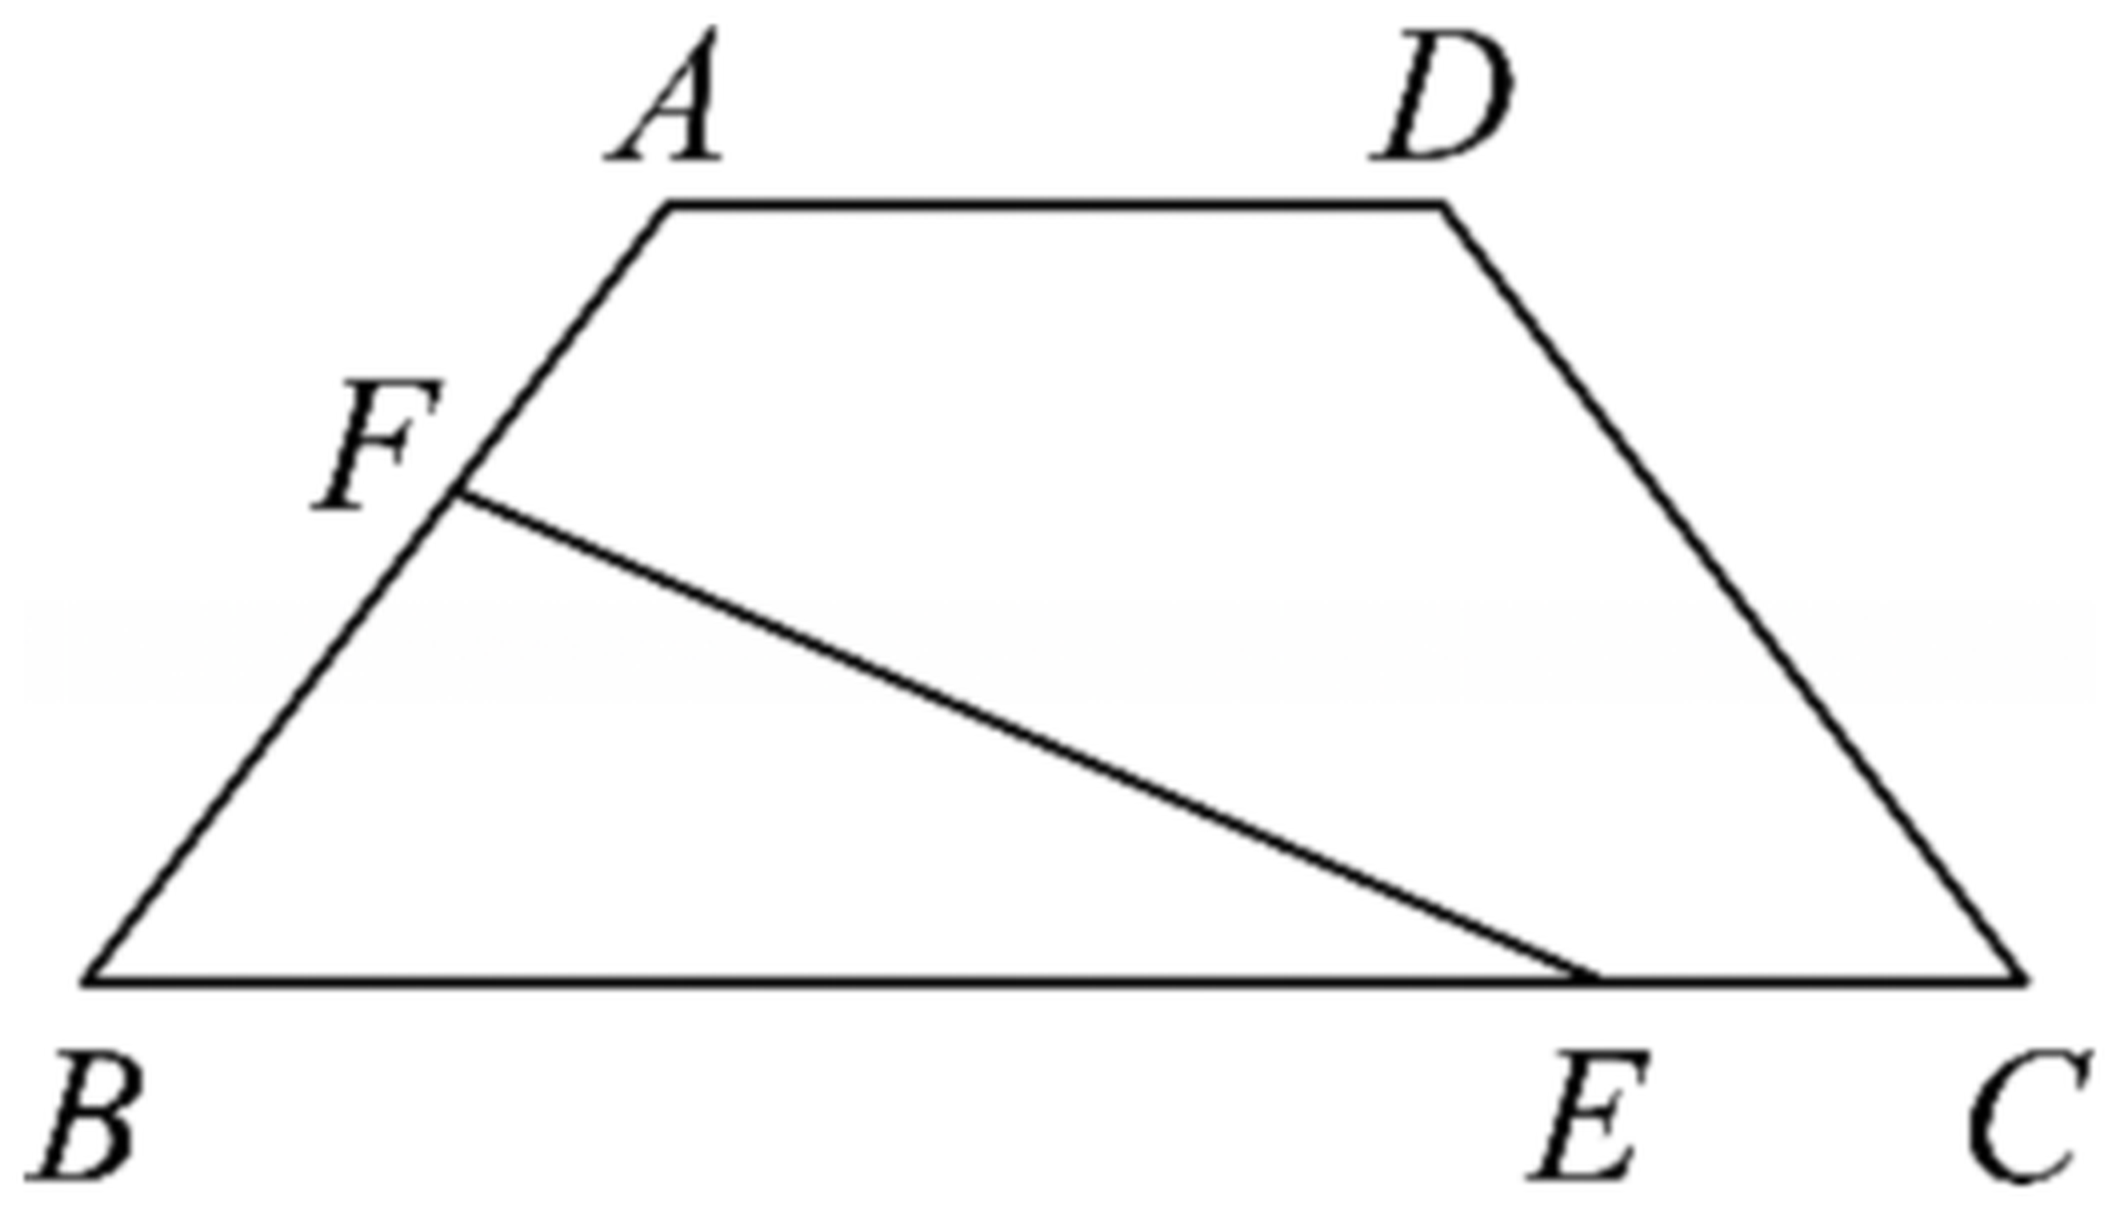
\includegraphics[width=0.46\textwidth]{figures/trapezoid_EF.png}
\end{center}

\begin{enumerate}[label=(\arabic*)]
\item 若 $EF$ 平分等腰梯形 $ABCD$ 的周长，设 $BE$ 长为 $x$，试用含 $x$ 的代数式表示
$\triangle BEF$ 的面积；
\item 是否存在线段 $EF$ 将等腰梯形 $ABCD$ 的周长和面积同时平分？若存在，求出此时 $BE$
的长；若不存在，请说明理由；
\item 是否存在线段 $EF$ 将等腰梯形 $ABCD$ 的周长和面积同时分成 $1:2$ 的两部分？
若存在，求此时 $BE$ 的长；若不存在，请说明理由.
\end{enumerate}

\ifanswer
\solbegin
\stepm{(1)}{过 $A$ 作 $AK\perp BC$ 交 $BC$ 于点 $K$，过 $F$ 作 $FG\perp BC$ 交 $BC$ 于点
$G$，}

\begin{center}
% 图取原卷截图、4× LANCZOS 放大（同梯形，多出虚线 $FG\perp BC$ 与 $AK\perp BC$
% 及两处直角符号；图只在【解析】里出现，故放进 \ifanswer 块）。
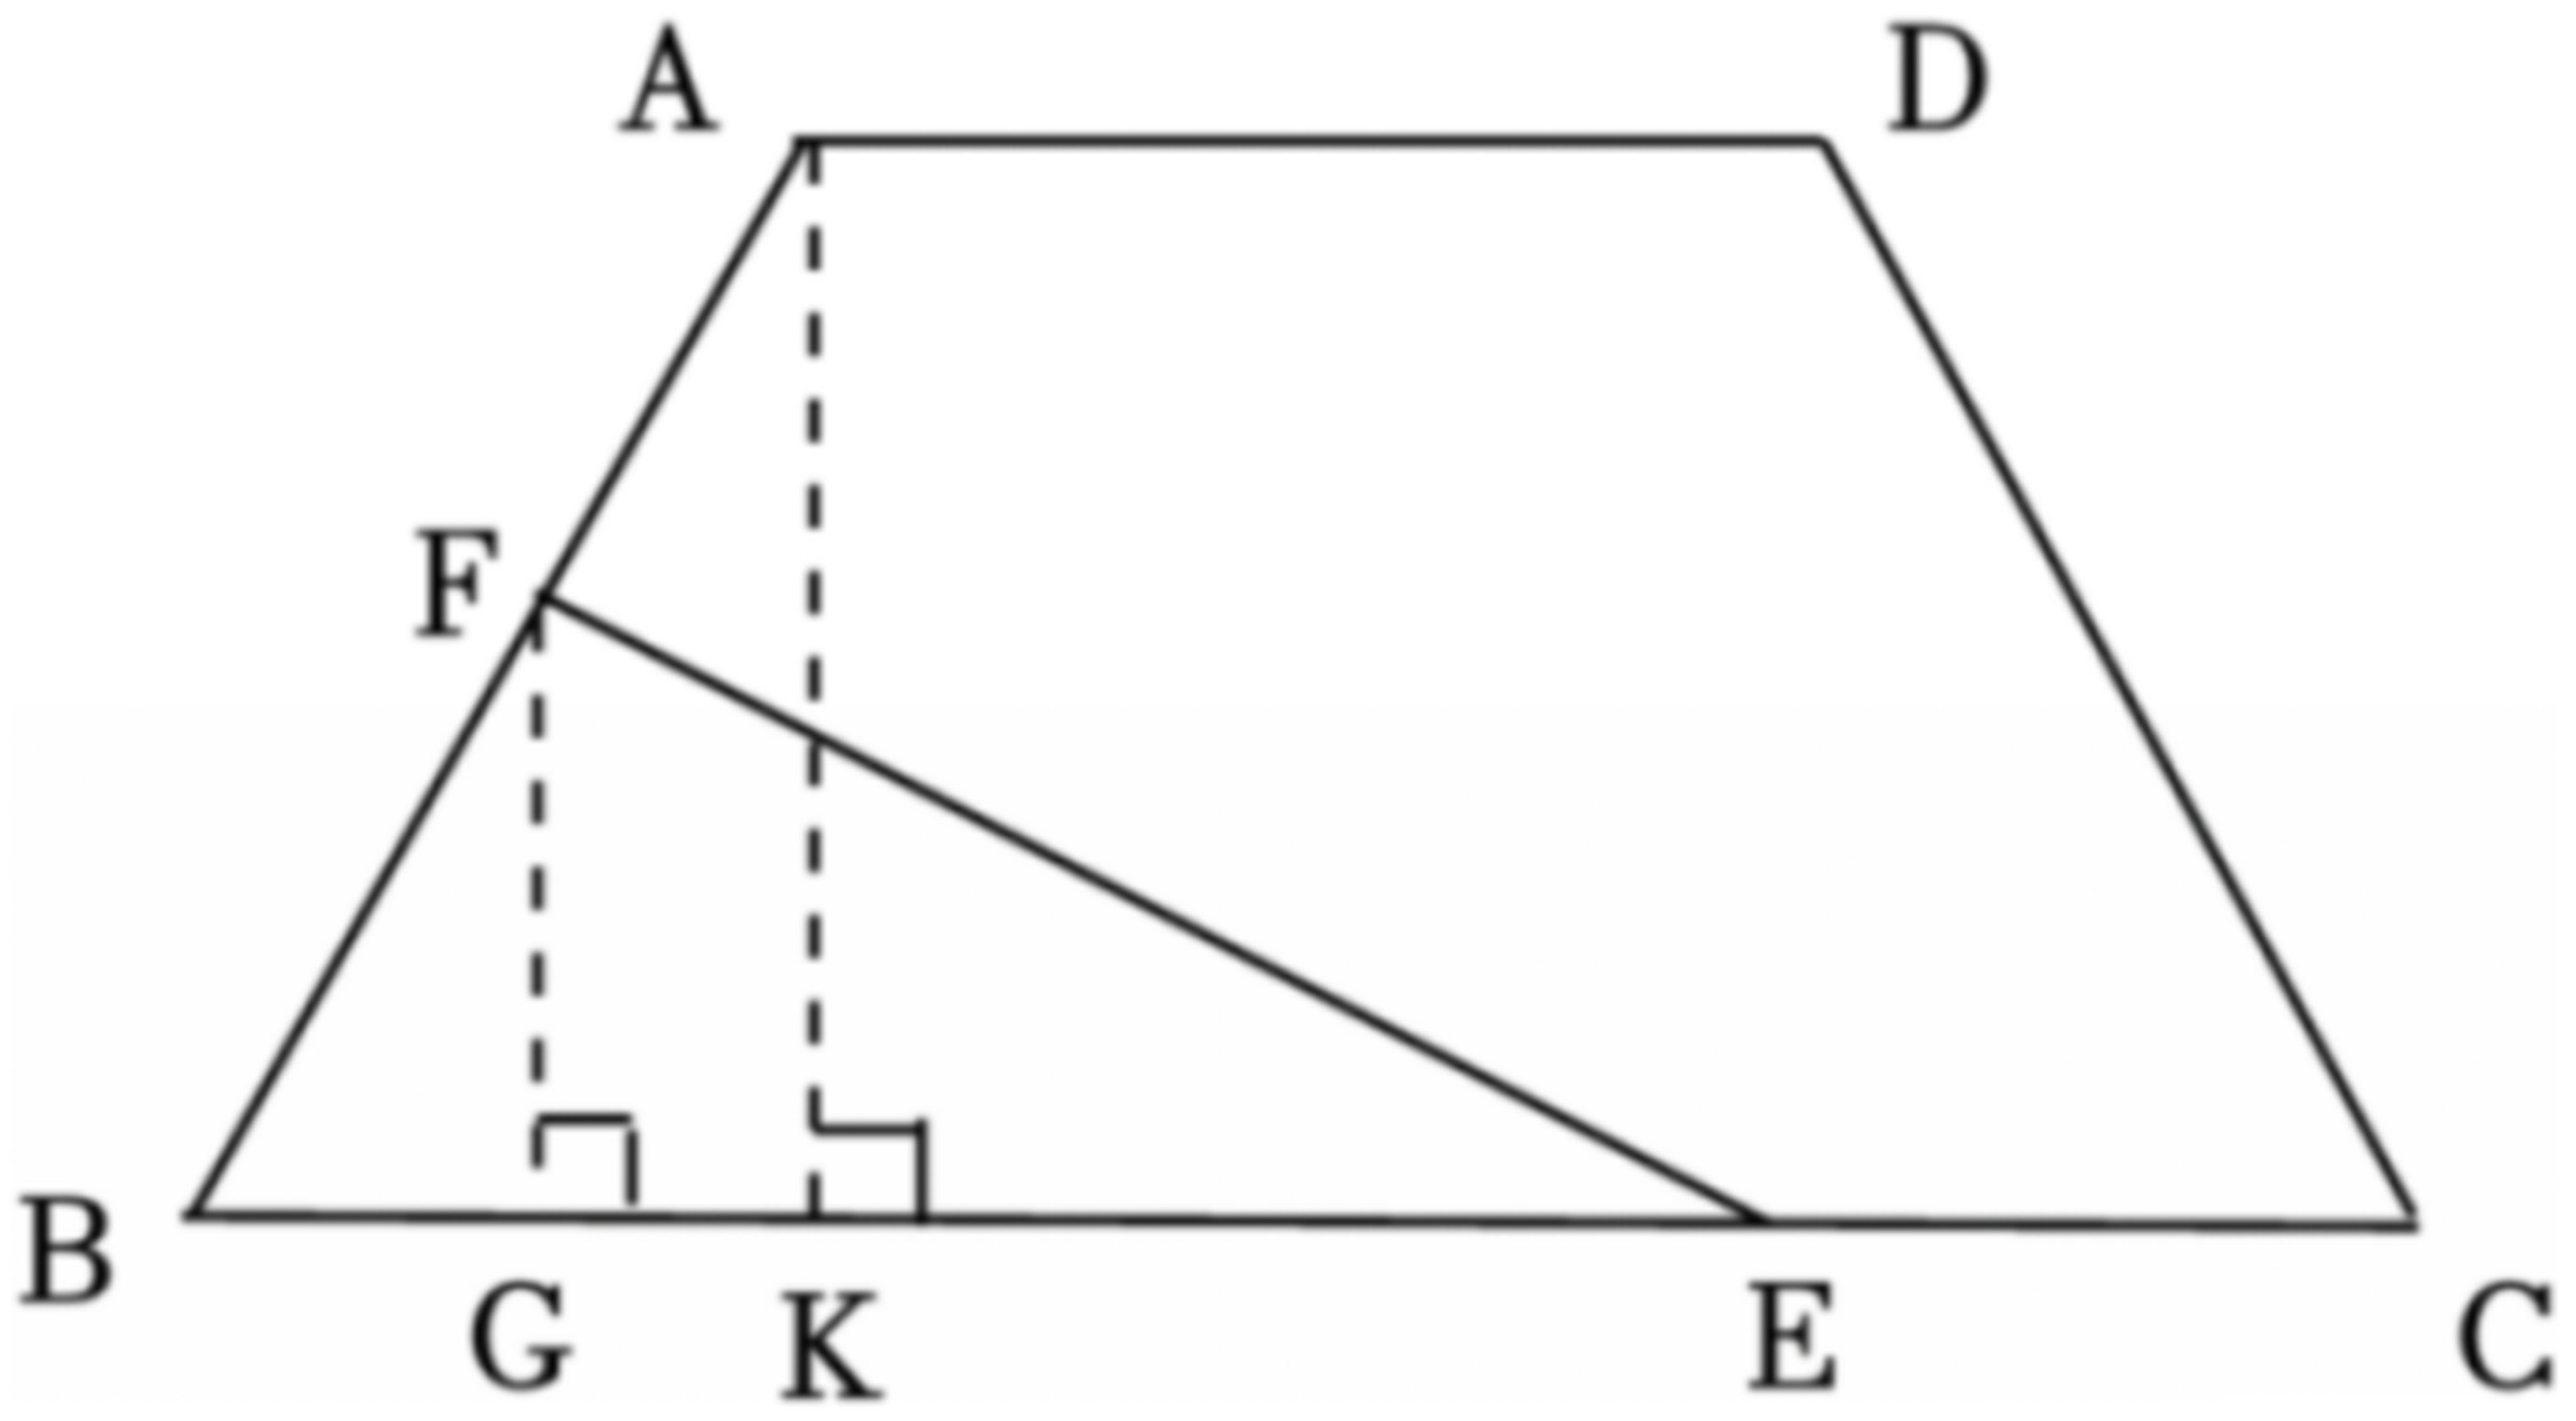
\includegraphics[width=0.62\textwidth]{figures/trapezoid_EF_aux.png}
\end{center}

\step{所以 $BK=\dfrac12\times(BC-AD)=\dfrac12\times(10-4)=3$，}
\step{$AK=\sqrt{AB^2-BK^2}=\sqrt{5^2-3^2}=4$，}
\step{由题意得，梯形 $ABCD$ 周长为 $24$，高为 $4$，面积为 $28$，}
\step{因为 $EF$ 平分等腰梯形 $ABCD$ 的周长，设 $BE$ 长为 $x$，则 $BF=12-x$，}
\step{由 $\begin{cases}0\leqslant12-x\leqslant5\\ 0\leqslant x\leqslant10\end{cases}$，
解得 $7\leqslant x\leqslant10$，}
\step{由题意得 $\triangle BFG\backsim\triangle BAK$，所以 $\dfrac{FG}{AK}=\dfrac{BF}{BA}$，
即 $\dfrac{FG}4=\dfrac{12-x}5$，}
\step{解得 $FG=\dfrac45(12-x)$，}
\step{所以 $S_{\triangle BEF}=\dfrac12BE\cdot FG
=-\dfrac25x^2+\dfrac{24}5x$（$7\leqslant x\leqslant10$）；}
\stepm{(2)}{存在，由 (1) 得 $-\dfrac25x^2+\dfrac{24}5x=\dfrac{28}2$，$x\in[7,10]$，}
\step{即 $x^2-12x+35=0$，解得 $x=7$ 或 $x=5$（舍去），}
\step{所以存在线段 $EF$ 将等腰梯形 $ABCD$ 的周长和面积同时平分，此时 $BE=7$；}
\stepm{(3)}{不存在，}
\step{情况一：$\triangle BEF$ 的面积$:$多边形 $AFECD$ 的面积 $=1:2$，
$(BE+BF):(AF+AD+DC+CE)=1:2$，}
\step{梯形周长的 $\dfrac13$ 是 $\dfrac{24}3=8$，面积的 $\dfrac13$ 是 $\dfrac{28}3$，}
\step{又因为 $BE=x$，所以 $BF=8-x$，}
\step{又因为 $\dfrac{FG}{AK}=\dfrac{BF}{BA}$，即 $\dfrac{FG}4=\dfrac{8-x}5$，
所以 $FG=\dfrac{32-4x}5$，}
\step{所以 $S_{\triangle BEF}=\dfrac12BE\times FG=-\dfrac25x^2+\dfrac{16}5x$，
所以 $\dfrac{28}3=-\dfrac25x^2+\dfrac{16}5x$，}
\step{整理得 $-3x^2+24x-70=0$，此时 $\Delta<0$，无解，故不存在；}
\step{情况二：$\triangle BEF$ 的面积$:$多边形 $AFECD$ 的面积 $=2:1$，
$(BE+BF):(AF+AD+DC+CE)=2:1$，}
\step{梯形周长的 $\dfrac13$ 为 $\dfrac{24}3=8$，面积的 $\dfrac13$ 为 $\dfrac{28}3$，
又 $BE=x$，所以 $BF=16-x$，}
\step{又 $\dfrac{FG}{AK}=\dfrac{BF}{BA}$，即 $\dfrac{FG}4=\dfrac{16-x}5$，
所以 $FG=\dfrac{64-4x}5$，}
\step{所以 $S_{\triangle BEF}=\dfrac12BE\times FG=-\dfrac25x^2+\dfrac{32}5x$，}
\step{所以 $\dfrac{28}3\times2=-\dfrac25x^2+\dfrac{32}5x$，
整理得 $-3x^2+48x-140=0$，}
\step{解得 $x=\dfrac{48+\sqrt{624}}6>10$，$x=\dfrac{48-\sqrt{624}}6<7$，
不符合题意，舍去，故不存在；}
\step{综上所述，不存在线段 $EF$ 将等腰梯形 $ABCD$ 的周长和面积同时分成 $1:2$ 的两部分.}
\solend

\fi

\ansspace[8]

\item 对集合 $\{1,2,\cdots,n\}$ 及其每一个非空子集 $A$，定义一个唯一确定的“交替和”
如下：将 $A$ 中的元素按照递减的次序排列，然后将第一个元素交替地减或加后继的元素所得的
结果，例如，子集 $\{1,2,4,6,9\}$ 的“交替和”是 $9-6+4-2+1=6$，子集 $\{5,6\}$ 的
“交替和”是 $6-5=1$，子集 $\{2\}$ 的交替和是 $2$；定义一个唯一确定的“交替积”如下：
将 $A$ 中的元素按照递减的次序排列，然后将第一个元素交替地除以或乘以后继的数所得的结果，
例如，集合 $\{1,2,4,6,9\}$ 的“交替积”是 $9\div6\times4\div2\times1=3$，
$\{5,6\}$ 的“交替积”是 $6\div5=1.2$，$\{2\}$ 的“交替积”是 $2$.

\begin{enumerate}[label=(\arabic*)]
\item 对于 $\{1,2,3,4,5,6,7,8,9\}$，求其所有子集的“交替和”的总和；
\item 对于 $\{1,2,\cdots,n\}$，求其所有子集的“交替和”的总和；
\item 对于 $\left\{n\mid\dfrac{495}{n+2}\in\N,n\in\Z\right\}$ 求其所有子集的
“交替积”的总和.
\end{enumerate}

\ifanswer
\solbegin
\stepm{(1)}{集合 $\{1,2,3,4,5,6,7,8,9\}$ 的子集中，除去 $\{9\}$ 外还有 $2^9-2$ 个
非空子集，}
\step{把这 $2^9-2$ 个非空子集两两组合后分别计算每一组中“交替和”之和，}
\step{组合原则是设 $A_i=\{9,a_1,a_2,\cdots\}$，$A_i^1=\{a_1,a_2,\cdots\}$，}
\step{集合 $A_i^1$ 的元素为集合 $A_i$ 中去掉 $9$ 的所有元素，把 $A_i$ 和 $A_i^1$
结合为一组，}
\step{显然，每组的“交替和”的和为 $9$，共有 $\dfrac{2^9-2}2$ 组，}
\step{所以，所有“交替和”之和应该为 $\dfrac{9(2^9-2)}2+9=2304$；}
\stepm{(2)}{集合 $\{1,2,\cdots,n\}$ 的子集中，除去 $\{n\}$ 外还有 $2^n-2$ 个非空子集，}
\step{把这 $2^n-2$ 个非空子集两两组合后分别计算每一组中“交替和”之和，}
\step{组合原则是设 $A_i=\{n,a_1,a_2,\cdots\}$，$A_i^1=\{a_1,a_2,\cdots\}$，}
\step{集合 $A_i^1$ 的元素为集合 $A_i$ 中去掉 $n$ 的所有元素，把 $A_i$ 和 $A_i^1$
结合为一组，}
\step{显然，每组的“交替和”的和为 $n$，共有 $\dfrac{2^n-2}2$ 组，}
% 注：下一行分子原卷印作花括号（其余同类处皆用圆括号），照抄未改，见文件头“原卷存疑”③。
\step{所以，所有“交替和”之和应该为 $\dfrac{n\{2^n-2\}}2+n=n\cdot2^{n-1}$；}
\stepm{(3)}{集合 $\left\{n\mid\dfrac{495}{n+2}\in\N,n\in\Z\right\}
=\{493,163,97,53,43,31,13,9,7,3,1,-1\}$，}
\step{其中除去 $\{-1\}$ 外还有 $2^{12}-2$ 个非空子集，}
% 注：下一行原卷把“把这”重复印了一次（“把这把这”），照抄未改，见文件头“原卷存疑”②。
\step{把这把这 $2^{12}-2$ 个非空子集两两组合后分别计算每一组中“交替积”之和，}
\step{组合原则是设 $A_j=\{-1,a_1,a_2,\cdots\}$，$A_j^1=\{a_1,a_2,\cdots\}$，}
\step{集合 $A_j^1$ 的元素为集合 $A_j$ 中去掉 $-1$ 的所有元素，把 $A_j$ 和 $A_j^1$
结合为一组，}
\step{显然，每组的“交替积”的和为 $0$，共有 $\dfrac{2^{12}-2}2$ 组，}
\step{所以，所有“交替积”之和应该为 $\dfrac{2^{12}-2}2\times0-1=-1$.}
\solend

\fi

\ansspace*[10]

\end{enumerate}

\end{document}
"
%
% 原始材料是微信公众号图文（公众号“魔都数学加油站”连载“27学年高一 30”，2026-09-23 发布，
% 原文标题“27学年高一30——2026-2027年上海市南洋模范中学高一上开学考”），
% 正文为 11 张 PNG 页。**同一篇里各页分辨率不一致**——第 2、3、9、10 页 4762×6735，
% 其余七页 2560×3620（已逐页打开确认，非下载缺档），取的是 mmbiz.qpic.cn/<hash>/0 的原图档。
% 原文本身就是一份**讲评版**：填空第 3—7 题下方印【答案】，第 8—12 题与其后各题印【解析】。
% 试题文字、答案与解析均照原卷录入，未改内容。卷面的粉色斜水印属水印，未录入。
%
% 卷首标题：原卷印作“2026-2027 年南洋模范中学高一上开学考”（公众号标题里的“上海市”
% 三字卷面标题行没有，本稿照卷面），年份区间按全稿惯例排 en dash，前缀照原卷保留“年”。
%
% 与原卷的排版差异（均已在 README“说明”中交代）：
%   ① 原文自**第 3 题**起（第 1、2 题未在该文中发布），故本稿题号亦自 3 起；
%   ② 原卷本就印有“一、填空题”“二、选择题”“三、解答题”三节标题，本稿照原卷分节，
%      只把标题改排成全稿统一的“大节标题”样式；
%   ③ 原卷填空第 3—7 题只印【答案】行、第 8 题起印【解析】（选择题答案写在解析末句
%      “故选 D／B”里），本稿统一改为试卷版隐去、答案版以 \ans{}／\ifanswer 块给出，
%      两版彻底分离；
%   ④ 子集符号原卷两种并用：第 7 题题干两处、第 19(2) 题作带下划线的 $\subseteq$，
%      第 17(2) 题解析作真包含的 $\subset$，本稿分别照录为 $\sub$ 与 $\subset$；
%   ⑤ 补集符号原卷一律作**上横线**（$\overline{A}$、$\overline{B}$），本稿照录；
%   ⑥ 原卷的实数集 R 一律作斜体（第 4 题、第 17 题与第 19 题题干的 $U=R$），
%      第 21(3) 题的自然数集与整数集作**粗体** $\mathbf{N}$、$\mathbf{Z}$，
%      本稿按全稿惯例统一写作 $\R$、$\N$、$\Z$；
%   ⑦ 原卷填空的横线约两个字宽，本稿按全稿惯例统一排 \blankline[4.4em]；
%   ⑧ 原卷未印副标题，本稿按全稿惯例补出副标题“集合与常用逻辑用语”——但本卷是开学考，
%      范围不止这一章：第 18 题是速度—时间图象题、第 20 题是等腰梯形的周长/面积平分问题，
%      副标题只标了主章节（见文末“高一30 专记”）；
%   ⑨ 第 13、14、18、20 题的图印在题干右侧、第 16 题的三幅图印在【解析】里的下一页顶部、
%      第 20 题【解析】另有一张带辅助线的图，本稿一律移至题干或解析之后；
%      图取原卷截图、4× LANCZOS 放大（见各 \includegraphics 前的注释）。
%
% 原卷存疑三处（均照抄原卷、未改，见源码中该处上方注释）：
%   ① 第 10 题【解析】验证“破晓集”时写的是 $\notin A$、$\in A$（如“$-2-2=-4\notin A$”），
%      但该处讨论的集合原题设里叫 $P$，同题②的“$x+y=2(k_1+k_2)\in A$”亦然——
%      本稿照抄未改（按文意应为 $P$）；
%   ② 第 21 题【解析】(3) 有“把这把这 $2^{12}-2$ 个非空子集”（“把这”重复印了一次）；
%   ③ 同题 (2) 的结论式分子原卷印作花括号 $\dfrac{n\{2^n-2\}}{2}$（其余同类处皆用圆括号）。

\documentclass[a4paper,11pt]{article}
\usepackage{common}

\begin{document}

\examtitlest[3]{2026--2027 年南洋模范中学高一上开学考}{集合与常用逻辑用语}

\bigsec{一、填空题}

\begin{enumerate}
\setcounter{enumi}{2}

\item 若集合 $A=\{x\mid x^2-2kx+7k=0\}$ 有且仅有三个真子集，则 $k$ 的取值范围是
\blankline[4.4em].

\ans{$(-\infty,0)\cup(7,+\infty)$}

\item “存在 $x\in\R$，使得 $x^2+2x+5=0$”的否定形式是 \blankline[4.4em].

\ans{对任何 $x\in\R$，都有 $x^2+2x+5\neq0$}

\item 下列命题中，$p$ 是 $q$ 的必要非充分条件的是 \blankline[4.4em].

① $p:x>2$ 且 $y>3$，$q:x+y>5$；

② $p$：四边形的四个角都相等，$q$：四边形是正方形.

\ans{②}

\item 若“条件 $\alpha:2\leqslant x\leqslant4$”是“条件 $\beta:3m-1\leqslant x\leqslant-m$”的
充分非必要条件，则 $m$ 的取值范围是 \blankline[4.4em].

\ans{$(-\infty,-4]$}

\item 满足 $\{1\}\sub M\sub\{1,2,4,5\}$ 的集合 $M$ 的个数为 \blankline[4.4em] 个.

\ans{$8$}

\item 已知集合 $A=\{1,2\}$，集合 $B=\{x\mid ax=6\}$，若 $A\cup B=A$，则 $a$ 的所有取值
构成的集合为 \blankline[4.4em].

\ifanswer
\solbegin
\step{因为 $A\cup B=A$，所以 $B\sub A$，}
\step{当 $a=0$ 时，$B=\varnothing$，满足 $B\sub A$；}
\step{当 $a\neq0$ 时，$B=\left\{\dfrac6a\right\}$，则 $\dfrac6a=1$ 或 $\dfrac6a=2$，
解得 $a=6$ 或 $a=3$，}
\step{综上所述，$a$ 的所有取值构成的集合为 $\{0,3,6\}$.}
\solend

\fi

\item 对于集合 $M$、$N$，定义 $M-N=\{x\mid x\in M\text{ 且 }x\notin N\}$，
$M\oplus N=(M-N)\cup(N-M)$，设 $A=\{y\mid y=|x|,x\in\R\}$，
$B=\{y\mid y=-(x-1)^2+2,x\in\R\}$，则 $A\oplus B=$ \blankline[4.4em].

\ifanswer
\solbegin
\step{由已知 $A=[0,+\infty)$，$B=(-\infty,2]$，}
\step{由于 $A-B=(2,+\infty)$，$B-A=(-\infty,0)$，}
\step{故 $A\oplus B=(A-B)\cup(B-A)=(-\infty,0)\cup(2,+\infty)$.}
\solend

\fi

\item 设 $P$ 为非空实数集满足：对任意给定的 $x$、$y\in P$（$x$、$y$ 可以相同），都有
$x+y\in P$，$x-y\in P$，$xy\in P$，则称 $P$ 为破晓集. 关于破晓集有下列结论：
①集合 $P=\{-2,-1,0,1,2\}$ 为破晓集；②集合 $P=\{x\mid x=2n,n\in\Z\}$ 为破晓集；
③若集合 $P_1$、$P_2$ 为破晓集，则 $P_1\cup P_2$ 为破晓集；④若集合 $P$ 为破晓集，
则一定有 $0\in P$；⑤若集合 $P_1$、$P_2$ 为破晓集，则 $P_1\cap P_2$ 为破晓集；
其中正确结论的序号是 \blankline[4.4em].

\ifanswer
\solbegin
% 注：以下几步原卷把该集合记作 $A$（题设里叫 $P$），照抄未改，见文件头“原卷存疑”①。
\step{对于①：$-2-2=-4\notin A$，故集合 $P=\{-2,-1,0,1,2\}$ 不为破晓集，故①错误；}
\step{②设 $x$、$y\in A$，则 $x=2k_1$，$y=2k_2$，且 $k_1$、$k_2\in\Z$，}
\step{故 $x+y=2(k_1+k_2)\in A$，$x-y=2(k_1-k_2)\in A$，$xy=4k_1k_2\in A$，}
\step{故集合 $P=\{x\mid x=2n,n\in\Z\}$ 为破晓集，故②正确；}
\step{③若集合 $P_1$、$P_2$ 为破晓集，设 $P_1=\{x\mid x=2k,k\in\Z\}$，
$P_2=\{x\mid x=3k,k\in\Z\}$，}
\step{但是 $P_1\cup P_2$ 不为破晓集，如 $x=2$，$y=3$ 时，$x+y=5$，
故 $5\notin(P_1\cup P_2)$，故③错误；}
\step{④若集合 $P$ 为破晓集，则取 $x=y$，$x-y=0\in A$，则一定有 $0\in P$，故④正确.}
\step{⑤正确；}
\step{故正确的是②④⑤.}
\solend

\fi

\item 已知集合 $M$ 的元素均为正整数，定义集合 $M$ 的“变项和”为：将 $M$ 中每个元素 $m$
都乘以 $(-1)^m$ 后再求和. 若集合 $A=\{n\mid1\leqslant n\leqslant10,n\in\N\}$，则集合 $A$
的所有非空子集的“变项和”的总和为 \blankline[4.4em].

\ifanswer
\solbegin
\step{$A$ 集合的所有非空子集中，每个元素出现的次数都是
$(2^{10}-1)-(2^9-1)=2^9$，}
\step{则集合 $A$ 的所有非空子集的“变项和”的总和为
$1\times(-1)^1\times2^9+2\times(-1)^2\times2^9+\cdots+10\times(-1)^{10}\times2^9$}
\step{$=(-1+2-3+4-\cdots-9+10)\times2^9=5\times2^9=2560$.}
\solend

\fi

\item 已知集合 $A=[t,t+1]\cup[t+4,t+9]$，$0\notin A$，存在正数 $\lambda$，使得对任意
$a\in A$，都有 $\dfrac\lambda a\in A$，则 $t$ 的值是 \blankline[4.4em].

\ifanswer
\solbegin
\step{当 $t>0$ 时，当 $a\in[t,t+1]$ 时，$\dfrac\lambda a\in[t+4,t+9]$，}
\step{当 $a\in[t+4,t+9]$ 时，$\dfrac\lambda a\in[t,t+1]$，}
\step{即当 $a=t$ 时，$\dfrac\lambda a\leqslant t+9$；当 $a=t+9$ 时，
$\dfrac\lambda a\geqslant t$，即 $\lambda=t(t+9)$；}
\step{当 $a=t+1$ 时，$\dfrac\lambda a\geqslant t+4$，当 $a=t+4$ 时，
$\dfrac\lambda a\leqslant t+1$，即 $\lambda=(t+1)(t+4)$，}
\step{所以 $t(t+9)=(t+1)(t+4)$，解得 $t=1$.}
\step{当 $t+1<0<t+4$ 时，当 $a\in[t,t+1]$ 时，$\dfrac\lambda a\in[t,t+1]$.}
\step{当 $a\in[t+4,t+9]$ 时，则 $\dfrac\lambda a\in[t+4,t+9]$，}
\step{即当 $a=t$ 时，$\dfrac\lambda a\leqslant t+1$，当 $a=t+1$ 时，
$\dfrac\lambda a\geqslant t$，即 $\lambda=t(t+1)$，}
\step{即当 $a=t+4$ 时，$\dfrac\lambda a\leqslant t+9$，当 $a=t+9$ 时，
$\dfrac\lambda a\geqslant t+4$，即 $\lambda=(t+4)(t+9)$，}
\step{所以 $t(t+1)=(t+4)(t+9)$，解得 $t=-3$.}
\step{当 $t+9<0$ 时，同理可得无解.}
\step{综上，$t$ 的值为 $1$ 或 $-3$.}
\solend

\fi

\end{enumerate}

\bigsec{二、选择题}

\begin{enumerate}
\setcounter{enumi}{12}

% 这道题是“题干 + 图 + 选项”约 6cm 的一整块，页末放不下就会被拆开（切页审计的 A 类），
% 故在题前先量一次页高：不够就把整道题干连图带选项一起挪到次页。
\needvspace{6.5cm}
\item 设 $U=\{1,2,3,4,5\}$，$A$、$B$ 都是 $U$ 的子集，且 $A\cap B=\{5\}$，
$\overline{A}\cap B=\{4\}$，$\overline{A}\cap\overline{B}=\{1,2\}$，
则以下四个判断中正确的是\mbox{（\quad）}

\begin{center}
% 图取原卷截图、4× LANCZOS 放大（原卷把图印在题干右侧，本稿移至此处，见文件头⑨）。
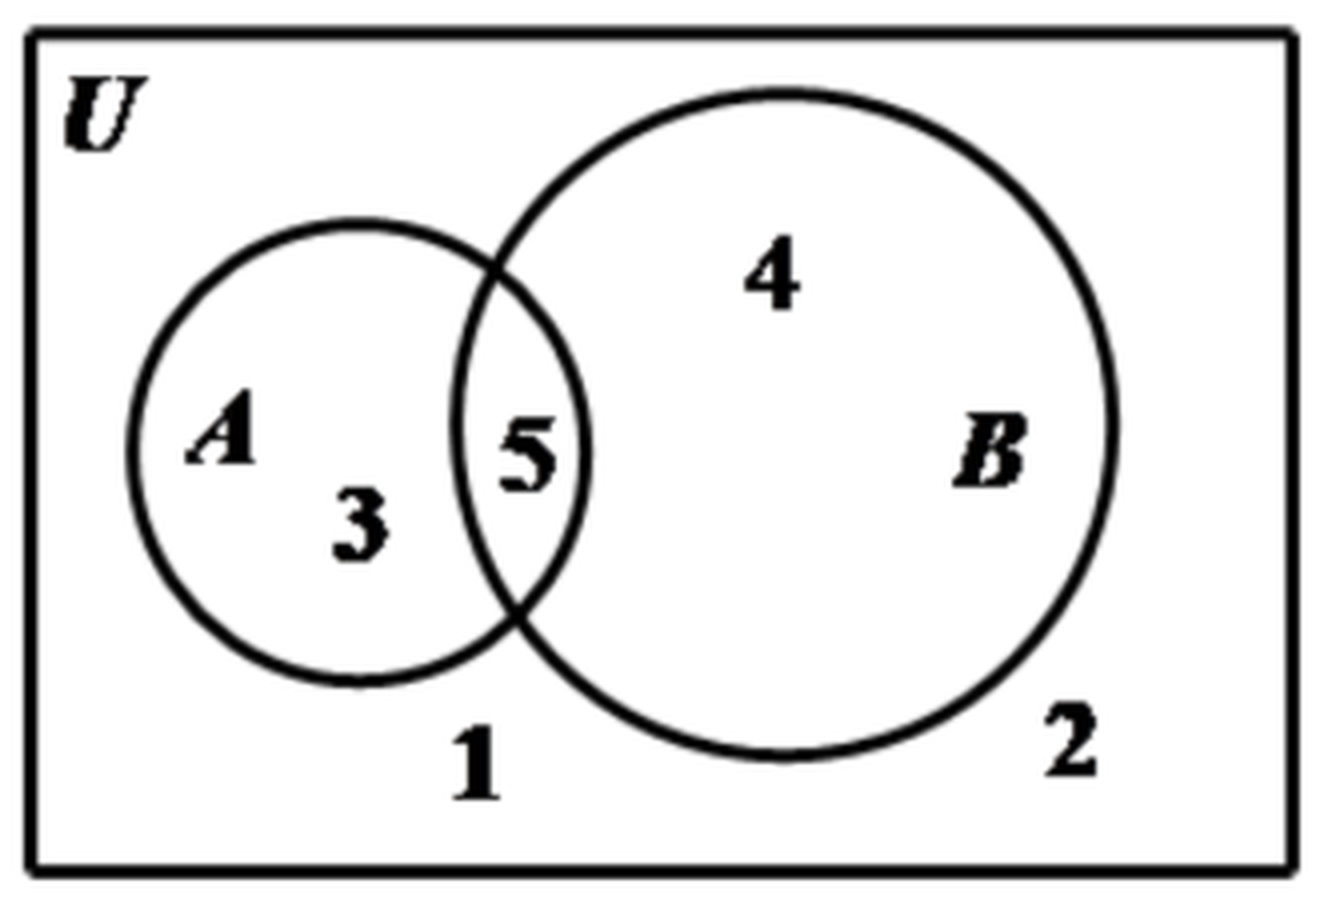
\includegraphics[width=0.28\textwidth]{figures/venn_U5_AB.png}
\end{center}

\keepwithprev
A. $3\notin A$ 且 $3\notin B$\qquad\qquad B. $3\in A$ 且 $3\in B$

C. $3\notin A$ 且 $3\in B$\qquad\qquad D. $3\in A$ 且 $3\notin B$

\ans{$D$}

\ifanswer
\solbegin
\step{画出韦恩图，得 $A=\{5,3\}$，$B=\{5,4\}$，}
\step{则 $3\in A$ 且 $3\notin B$. 故选 $D$.}
\solend

\fi

% 同第 13 题：整块（题干 + 图 + 选项）在答案版还要再挂【答案】【解析】，页末更易被拆开。
\needvspace{7.5cm}
\item 如图表示图形阴影部分的是\mbox{（\quad）}

\begin{center}
% 图取原卷截图、4× LANCZOS 放大（三圆 $A$、$B$、$C$，阴影为整个 $A$ 圆加 $B\cap C$）。
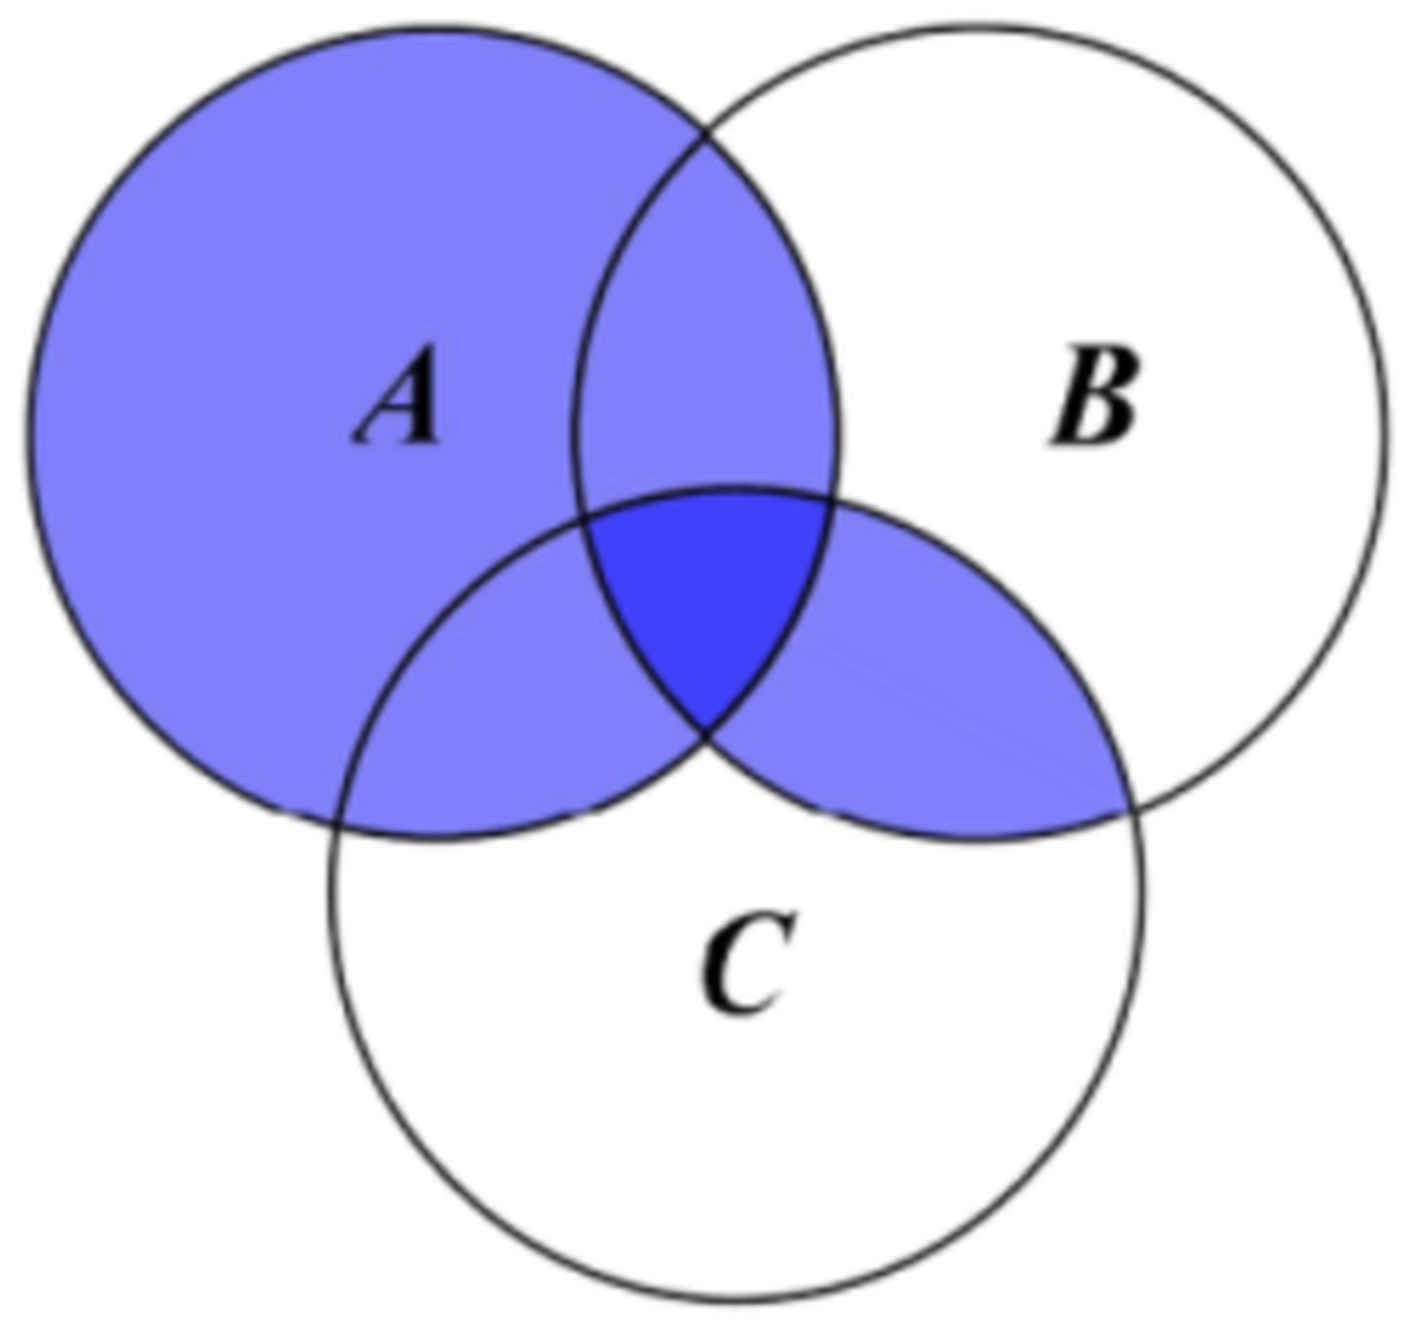
\includegraphics[width=0.30\textwidth]{figures/venn_A_union_BC.png}
\end{center}

\keepwithprev
A. $(A\cup C)\cap(B\cup C)$\qquad\qquad B. $(A\cup B)\cap(A\cup C)$

C. $(A\cup B)\cap(B\cup C)$\qquad\qquad D. $(A\cup B)\cap C$

\ans{$B$}

\ifanswer
\solbegin
\step{图中阴影部分表示元素满足是 $A$ 中的元素，或者是 $B$ 与 $C$ 的公共元素，}
\step{故可以表示为 $A\cup(B\cap C)$，也可以表示为 $(A\cup B)\cap(A\cup C)$.
故选 $B$.}
\solend

\fi

\item 设集合 $M=\left\{x\mid m\leqslant x\leqslant m+\dfrac34\right\}$，
$N=\left\{x\mid n-\dfrac13\leqslant x\leqslant n\right\}$，且 $M$、$N$ 都是集合
$\{x\mid0\leqslant x\leqslant1\}$ 的子集，如果把 $b-a$ 叫做集合
$\{x\mid a\leqslant x\leqslant b\}$ 的“长度”，那么集合 $M\cap N$ 的“长度”的
最小值是\mbox{（\quad）}

\keepwithprev
A. $\dfrac23$\qquad B. $\dfrac1{12}$\qquad C. $\dfrac13$\qquad D. $\dfrac5{12}$

\ans{$B$}

\ifanswer
\solbegin
\step{$M$ 的长度为 $\dfrac34$，$N$ 的长度为 $\dfrac13$，}
\step{当集合 $M\cap N$ 的长度的最小值时，$M$ 与 $N$ 应分别在区间 $[0,1]$ 的左右两端，}
\step{故 $M\cap N$ 的长度的最小值是 $\dfrac34+\dfrac13-1=\dfrac1{12}$，故选 $B$.}
\solend

\fi

\item 定义集合运算 $A-B=\{x\mid x\in A\text{ 且 }x\notin B\}$ 称为集合 $A$ 与集合 $B$ 的
差集；定义集合运算 $A\Delta B=(A-B)\cup(B-A)$ 称为集合 $A$ 与集合 $B$ 的对称差，
有以下 $4$ 个等式：① $A\Delta B=B\Delta A$；② $(A\Delta B)\Delta C=A\Delta(B\Delta C)$；
③ $A\cap(B\Delta C)=(A\cap B)\Delta(A\cap C)$；
④ $A\cup(B\Delta C)=(A\cup B)\Delta(A\cup C)$，
则 $4$ 个等式中恒成立的是\mbox{（\quad）}

\keepwithprev
A. ①②\qquad B. ①②③\qquad C. ①②④\qquad D. ①②③④

\ans{$B$}

\ifanswer
\solbegin
\step{对于①，由 $B\Delta A=(B-A)\cup(A-B)=(A-B)\cup(B-A)=A\Delta B$，
所以①正确；}
\step{对于②，由 $A-B=\{x\mid x\in A\text{ 且 }x\notin B\}
=\{x\mid x\in A,x\notin(A\cap B)\}=A-(A\cap B)$，}
\step{同理可得 $B-A=B-(A\cap B)$，}
\step{则 $A\Delta B=(A-B)\cup(B-A)=(A\cup B)-(A\cap B)$，}
\step{所以 $(A\Delta B)\Delta C=(A\Delta B)\cup C-(A\Delta B)\cap C$，}
\step{所以表示的集合为图（1）中阴影部分所表示的集合，如图所示，}
\step{同理 $A\Delta(B\Delta C)=A\cup(B\Delta C)-A\cap(B\Delta C)$，
也表示图（1）中阴影部分所表示的集合，}
\step{所以 $(A\Delta B)\Delta C=A\Delta(B\Delta C)$，所以②正确；}

\begin{center}
% 图取原卷截图、4× LANCZOS 放大（原卷印在下一页顶部，共三幅三圆韦恩图：
% 图（1）一幅、图（2）左右两幅，图（2）两幅下方各有一行式子标注）。
% 图只在【解析】里出现，故放进 \ifanswer 块，试卷版不排。
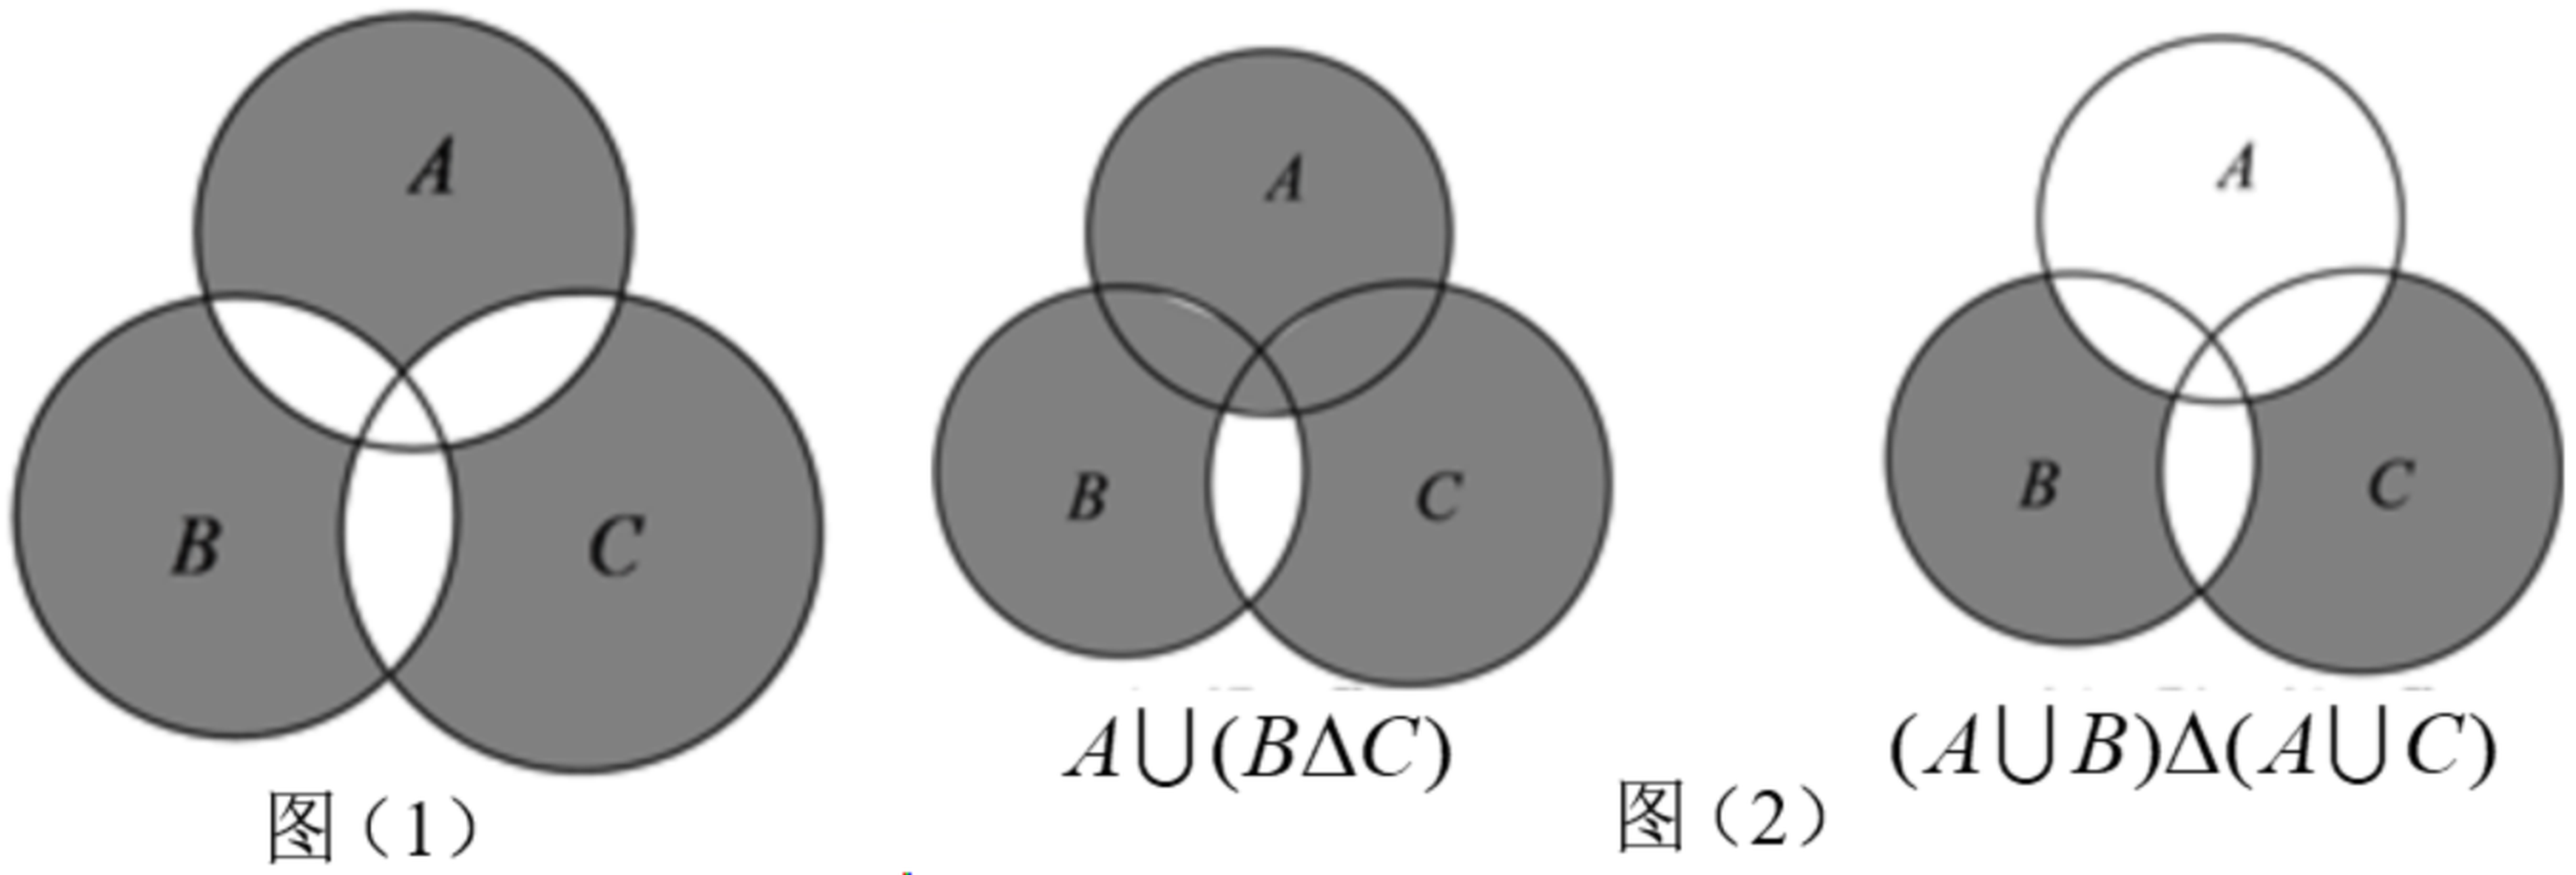
\includegraphics[width=0.86\textwidth]{figures/venn_symdiff3.png}
\end{center}

\step{对于③，由 $A\cap(B\Delta C)=A\cap(B\cup C-B\cap C)
=A\cap(B\cup C)-A\cap(B\cap C)$}
\step{$=(A\cap B)\cup(A\cap C)-(A\cap B)\cap(A\cap C)=(A\cap B)\Delta(A\cap C)$，
所以③正确；}
\step{对于④，如图（2）所示，$A\cup(B\Delta C)\neq(A\cup B)\Delta(A\cup C)$，
所以④错误.}
\step{故选 $B$.}
\solend

\fi

\end{enumerate}

\bigsec{三、解答题}

\begin{enumerate}
\setcounter{enumi}{16}

\item 已知集合 $M=\{x\mid a-1\leqslant x\leqslant2a+3\}$，$P=\{x\mid-2<x\leqslant4\}$，
全集 $U=\R$.

\begin{enumerate}[label=(\arabic*)]
\item 当 $a=2$ 时，求 $M\cap P$；
\item 若 $x\in P$ 是 $x\in M$ 的必要不充分条件，求实数 $a$ 的取值范围.
\end{enumerate}

\ifanswer
\solbegin
\stepm{(1)}{当 $a=2$ 时，集合 $M=\{x\mid1\leqslant x\leqslant7\}$，}
\step{所以 $M\cap P=\{x\mid1\leqslant x\leqslant4\}$；}
\stepm{(2)}{因为 $x\in P$ 是 $x\in M$ 的必要不充分条件，所以 $M\subset P$，}
\step{当 $M=\varnothing$ 时，$a-1>2a+3$，解得 $a<-4$，}
\step{当 $M\neq\varnothing$ 时，则
$\begin{cases}a-1\leqslant2a+3\\ a-1>-2\\ 2a+3\leqslant4\end{cases}$，
解得 $-1<a\leqslant\dfrac12$，}
\step{综上所述，实数 $a$ 的取值范围为
$(-\infty,-4)\cup\left(-1,\dfrac12\right]$.}
\solend

\fi

\ansspace[6]

\item 一辆汽车在某段路程中的行驶速度与时间的关系如图：

\begin{center}
% 图取原卷截图、4× LANCZOS 放大（速度—时间图：纵轴 $v/(\mathrm{km/h})$、
% 横轴 $t(\mathrm{h})$，$t\in[0,1]$、$[1,2]$、$[2,3]$ 三段矩形条高 50、80、90）。
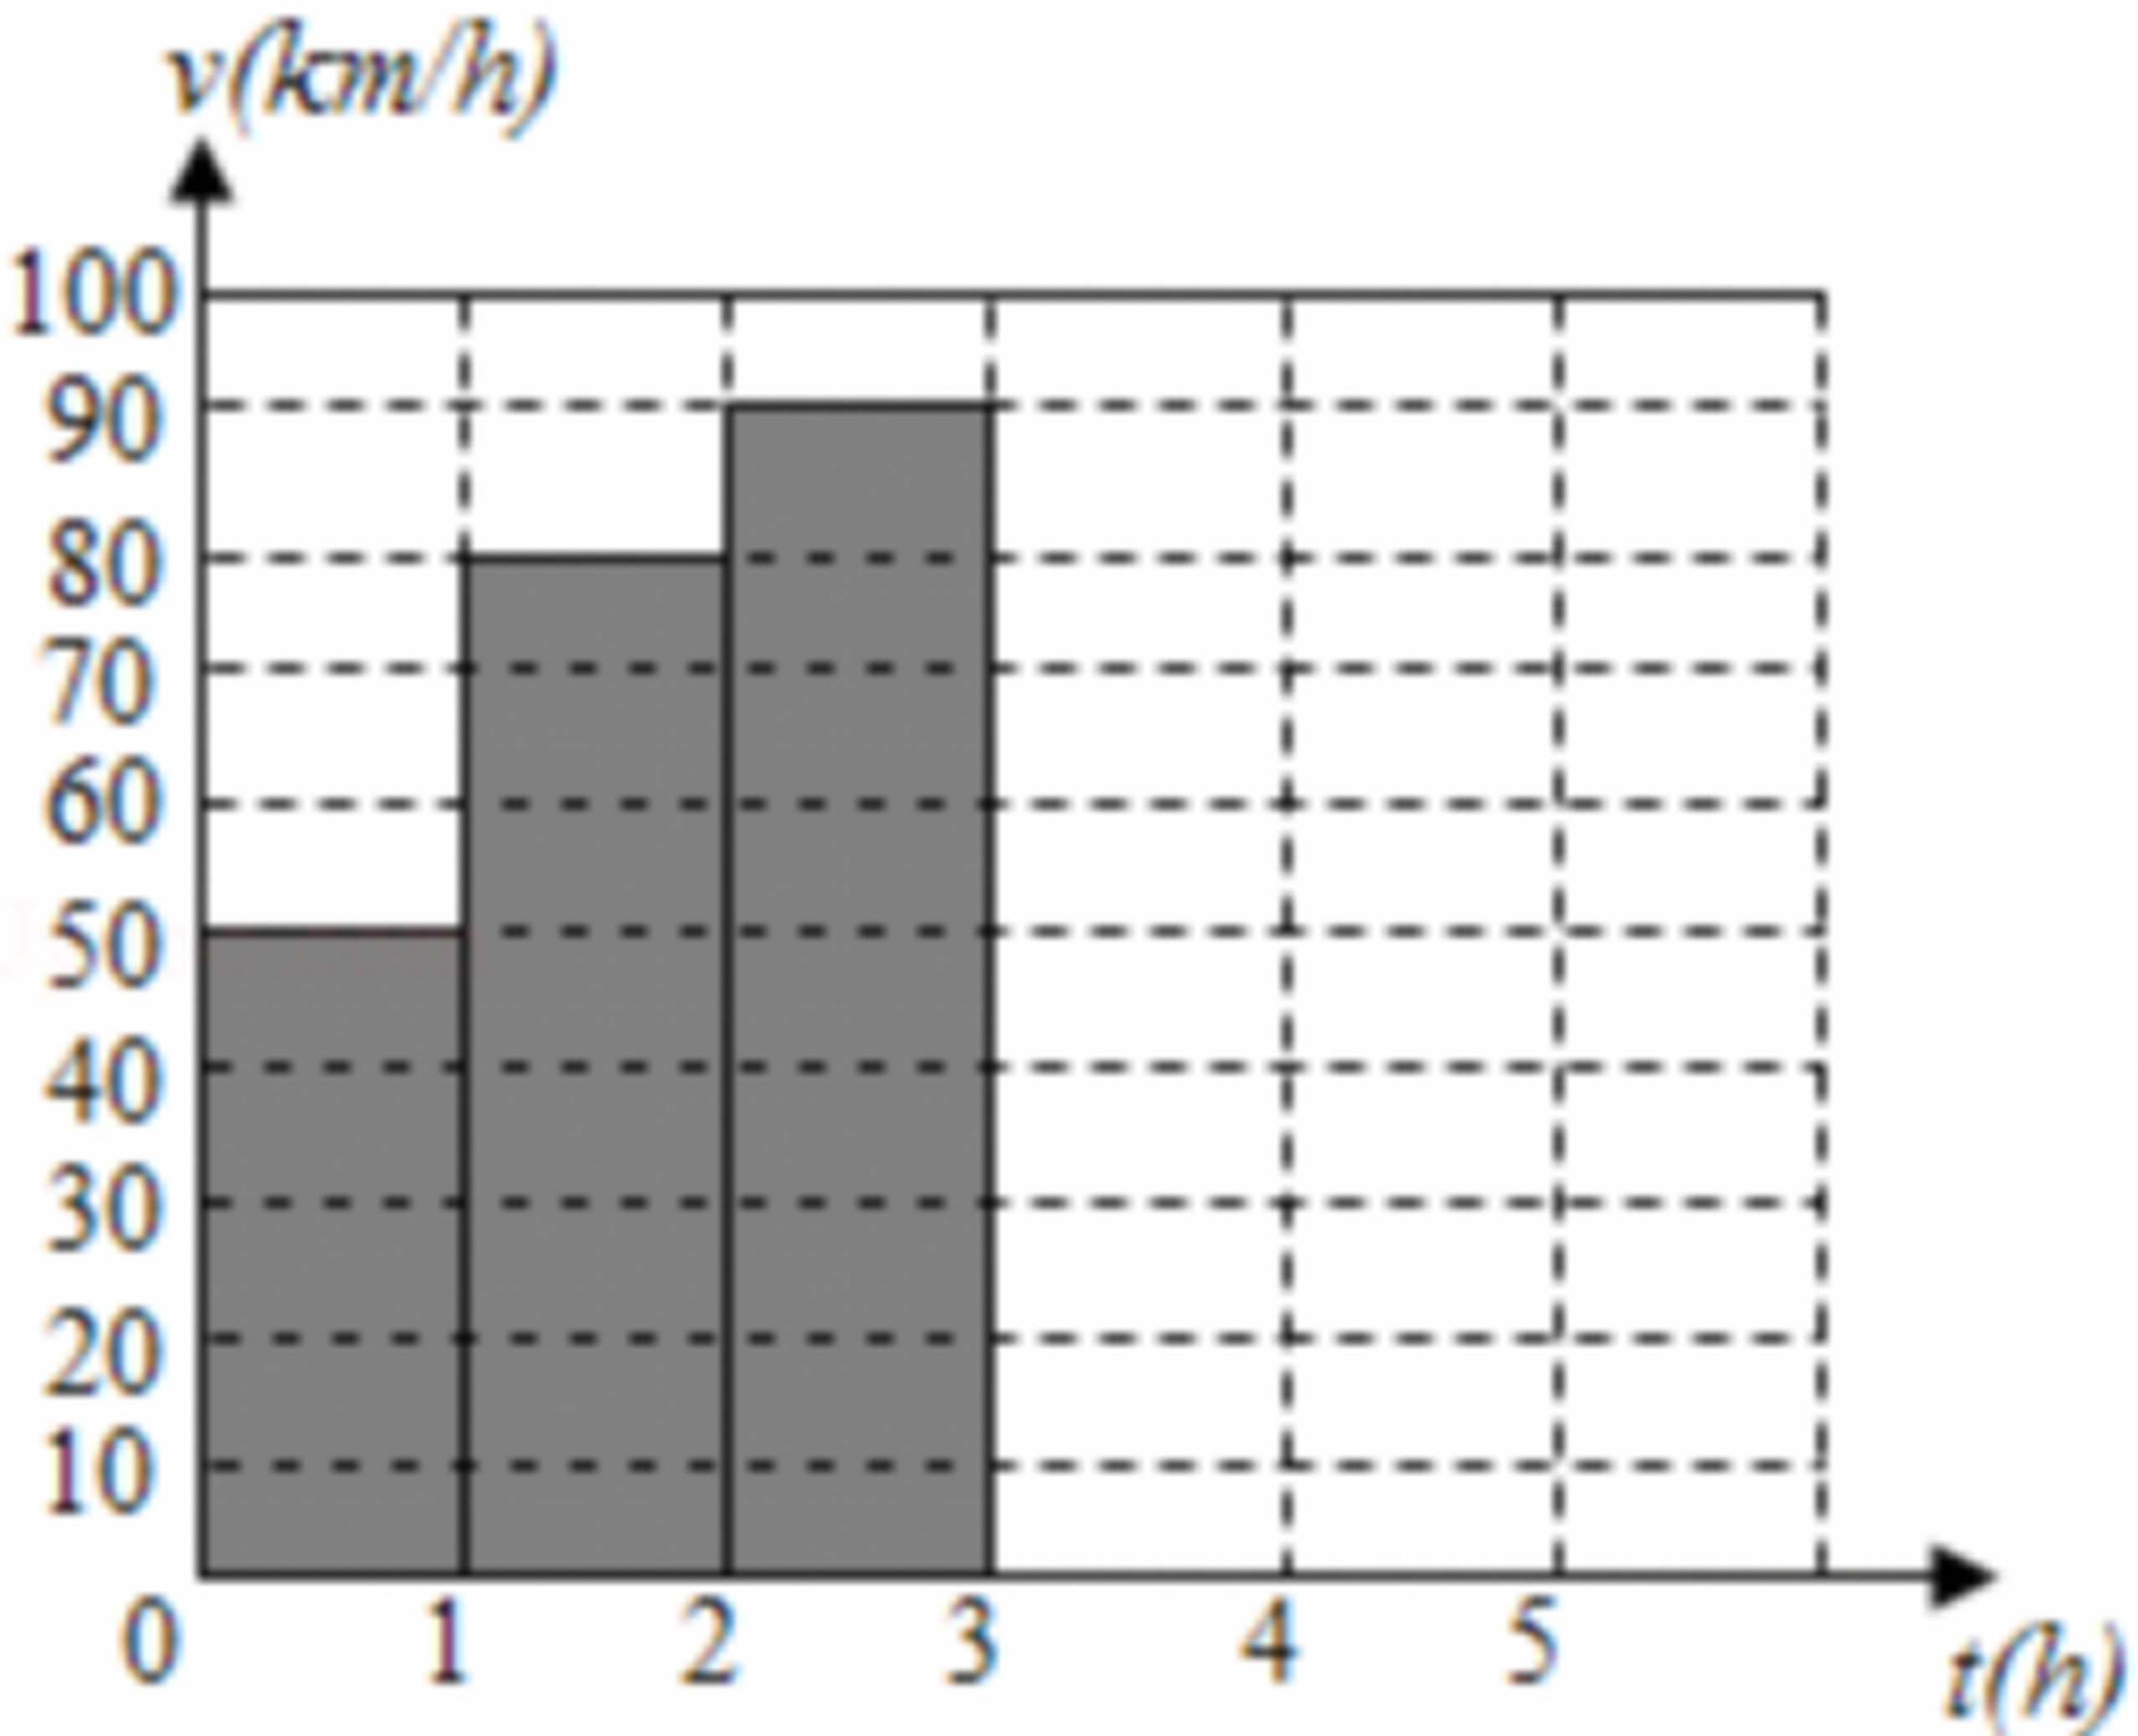
\includegraphics[width=0.52\textwidth]{figures/speed_time_bars.png}
\end{center}

\begin{enumerate}[label=(\arabic*)]
\item 求图中阴影部分的面积，并说明所求面积的实际意义；
\item 假设这辆汽车的里程表在汽车行驶这段路程前的读数为 $2004\,\mathrm{km}$，
试将汽车行驶这段路程时汽车里程表读数 $S$ 表示为时间 $t$ 的函数，
并求出当汽车里程表读数为 $2094\,\mathrm{km}$ 时，汽车行驶了多少时间？
\end{enumerate}

\ifanswer
\solbegin
\stepm{(1)}{由一辆汽车在某段路程中的行驶速度与时间的关系图，}
\step{得阴影部分的面积为 $50\times1+80\times1+90\times1=220$，}
\step{阴影部分的面积表示汽车在 $3$ 小时内行驶的路程为 $220\,\mathrm{km}$.}
\stepm{(2)}{$S=\begin{cases}
50t+2004,&0\leqslant t<1\\
80(t-1)+2054,&1\leqslant t<2\\
90(t-2)+2134,&2\leqslant t\leqslant3
\end{cases}$}
\step{令 $80(t-1)+2054=2094$，解得 $t=1.5$，所以汽车行驶 $1.5$ 小时.}
\solend

\fi

\ansspace[6]

\item 已知集合 $A=\{x\mid x<-2\text{ 或 }x\geqslant3\}$，$U=\R$.

\begin{enumerate}[label=(\arabic*)]
\item 求 $\overline{A}$；
\item 若 $B=\{x\mid mx-1>0\}$，当 $B\sub A$ 时，求实数 $m$ 的取值范围；
\item 若 $B=\{x\mid2m-6\leqslant x\leqslant m+4\}$，当 $B\cap\overline{A}=\varnothing$ 时，
求实数 $m$ 的取值范围.
\end{enumerate}

\ifanswer
\solbegin
\stepm{(1)}{因为集合 $A=\{x\mid x<-2\text{ 或 }x\geqslant3\}$，$U=\R$，
所以 $\overline{A}=\{x\mid-2\leqslant x<3\}$；}
\stepm{(2)}{当 $m=0$ 时，$B=\varnothing$，符合题意，}
\step{当 $m>0$ 时，$B=\left\{x\mid x>\dfrac1m\right\}$，则 $\dfrac1m\geqslant3$，
解得 $0<m\leqslant\dfrac13$，}
\step{当 $m<0$ 时，$B=\left\{x\mid x<\dfrac1m\right\}$，则 $\dfrac1m\leqslant-2$，
解得 $-\dfrac12\leqslant m<0$，}
\step{综上所述，实数 $m$ 的取值范围 $\left[-\dfrac12,\dfrac13\right]$；}
\stepm{(3)}{由题意得 $B=\{x\mid2m-6\leqslant x\leqslant m+4\}$，
$\overline{A}=\{x\mid-2\leqslant x<3\}$，且 $B\cap\overline{A}=\varnothing$，}
\step{当 $B=\varnothing$ 时，$2m-6>m+4$，解得 $m>10$，}
\step{当 $B\neq\varnothing$ 时，则 $\begin{cases}2m-6\leqslant m+4\\ m+4<-2\end{cases}$
或 $\begin{cases}2m-6\leqslant m+4\\ 2m-6\geqslant3\end{cases}$，}
\step{解得 $m<-6$ 或 $\dfrac92\leqslant m\leqslant10$，}
\step{综上所述，实数 $m$ 的取值范围为
$(-\infty,-6)\cup\left[\dfrac92,+\infty\right)$.}
\solend

\fi

\ansspace[8]

\item 在等腰梯形 $ABCD$ 中，$AB=DC=5$，$AD=4$，$BC=10$. 点 $E$ 在下底边 $BC$ 上.
点 $F$ 在腰 $AB$ 上.

\begin{center}
% 图取原卷截图、4× LANCZOS 放大（等腰梯形 $ABCD$ 与线段 $FE$，无辅助线）。
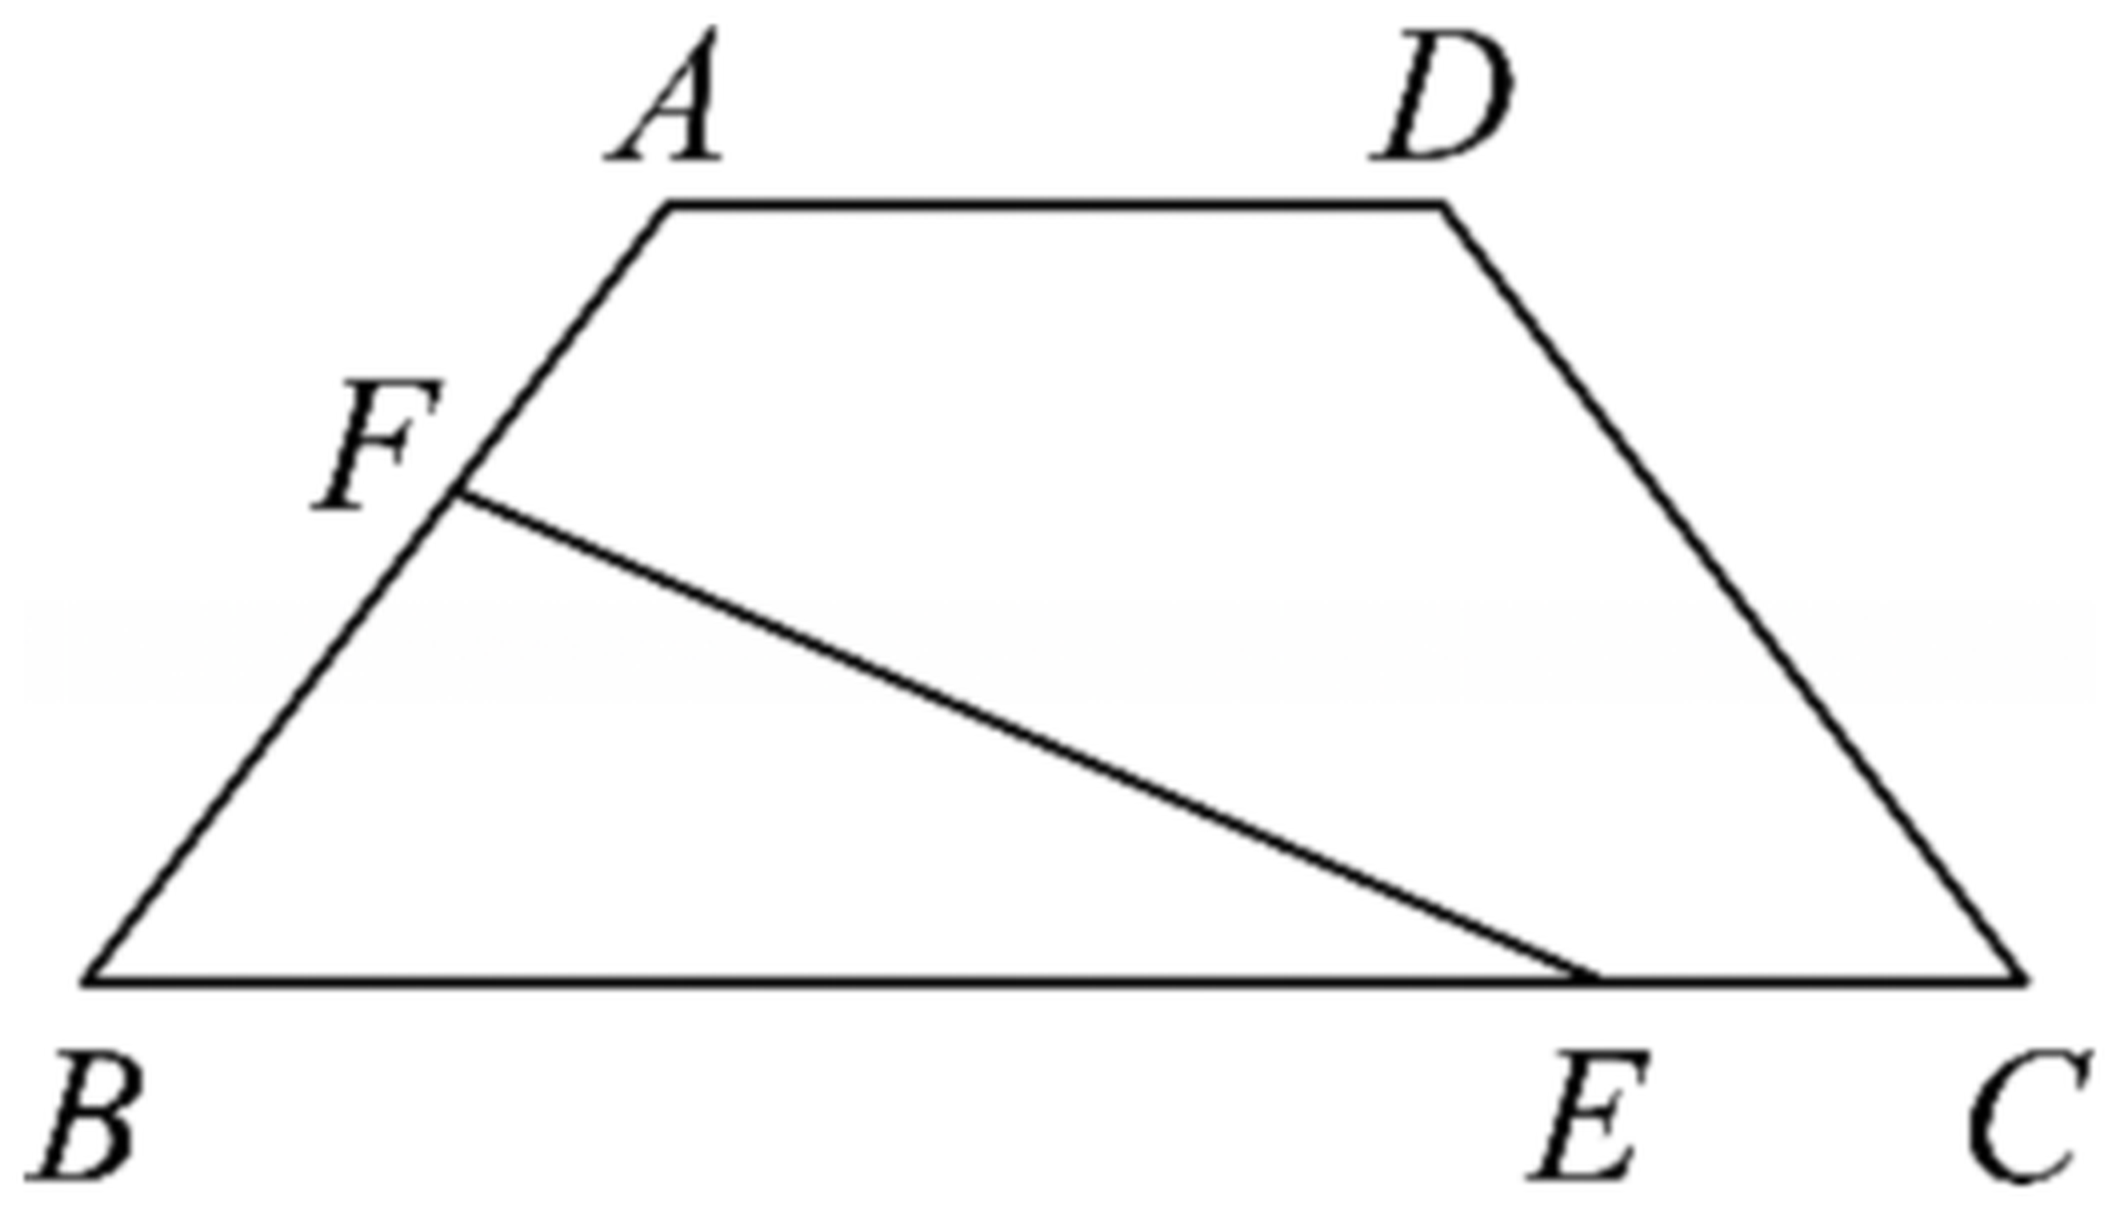
\includegraphics[width=0.46\textwidth]{figures/trapezoid_EF.png}
\end{center}

\begin{enumerate}[label=(\arabic*)]
\item 若 $EF$ 平分等腰梯形 $ABCD$ 的周长，设 $BE$ 长为 $x$，试用含 $x$ 的代数式表示
$\triangle BEF$ 的面积；
\item 是否存在线段 $EF$ 将等腰梯形 $ABCD$ 的周长和面积同时平分？若存在，求出此时 $BE$
的长；若不存在，请说明理由；
\item 是否存在线段 $EF$ 将等腰梯形 $ABCD$ 的周长和面积同时分成 $1:2$ 的两部分？
若存在，求此时 $BE$ 的长；若不存在，请说明理由.
\end{enumerate}

\ifanswer
\solbegin
\stepm{(1)}{过 $A$ 作 $AK\perp BC$ 交 $BC$ 于点 $K$，过 $F$ 作 $FG\perp BC$ 交 $BC$ 于点
$G$，}

\begin{center}
% 图取原卷截图、4× LANCZOS 放大（同梯形，多出虚线 $FG\perp BC$ 与 $AK\perp BC$
% 及两处直角符号；图只在【解析】里出现，故放进 \ifanswer 块）。
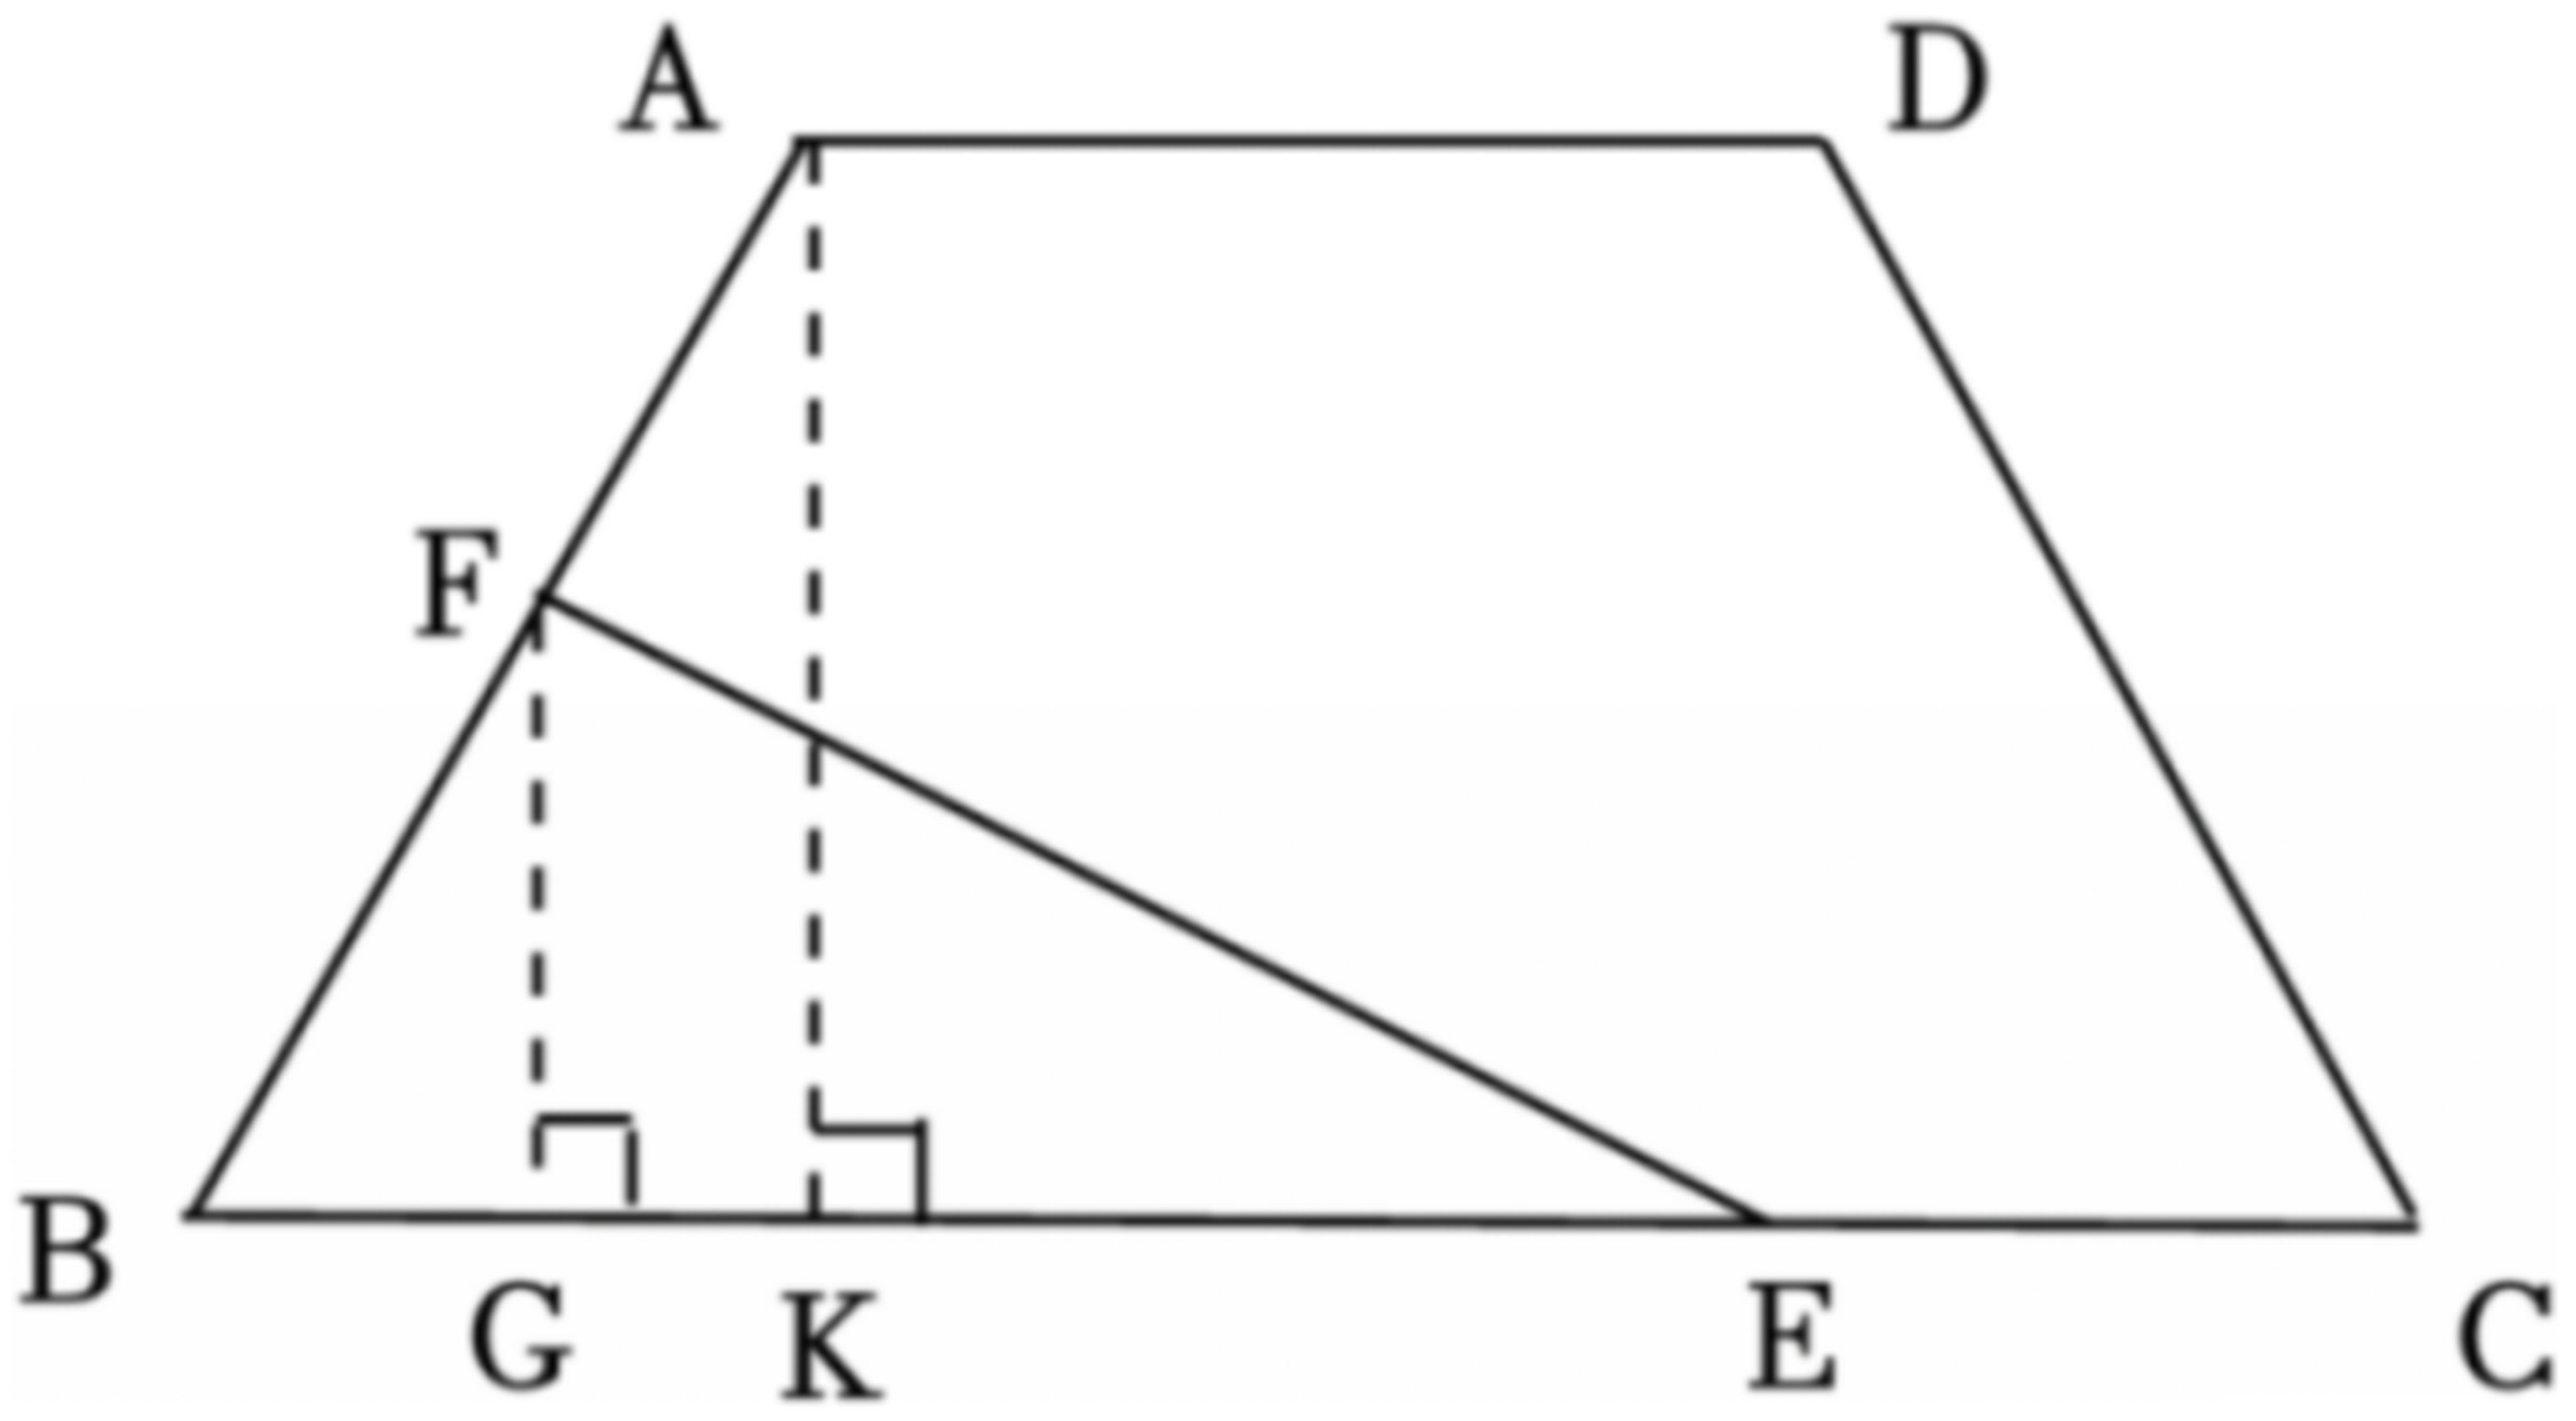
\includegraphics[width=0.62\textwidth]{figures/trapezoid_EF_aux.png}
\end{center}

\step{所以 $BK=\dfrac12\times(BC-AD)=\dfrac12\times(10-4)=3$，}
\step{$AK=\sqrt{AB^2-BK^2}=\sqrt{5^2-3^2}=4$，}
\step{由题意得，梯形 $ABCD$ 周长为 $24$，高为 $4$，面积为 $28$，}
\step{因为 $EF$ 平分等腰梯形 $ABCD$ 的周长，设 $BE$ 长为 $x$，则 $BF=12-x$，}
\step{由 $\begin{cases}0\leqslant12-x\leqslant5\\ 0\leqslant x\leqslant10\end{cases}$，
解得 $7\leqslant x\leqslant10$，}
\step{由题意得 $\triangle BFG\backsim\triangle BAK$，所以 $\dfrac{FG}{AK}=\dfrac{BF}{BA}$，
即 $\dfrac{FG}4=\dfrac{12-x}5$，}
\step{解得 $FG=\dfrac45(12-x)$，}
\step{所以 $S_{\triangle BEF}=\dfrac12BE\cdot FG
=-\dfrac25x^2+\dfrac{24}5x$（$7\leqslant x\leqslant10$）；}
\stepm{(2)}{存在，由 (1) 得 $-\dfrac25x^2+\dfrac{24}5x=\dfrac{28}2$，$x\in[7,10]$，}
\step{即 $x^2-12x+35=0$，解得 $x=7$ 或 $x=5$（舍去），}
\step{所以存在线段 $EF$ 将等腰梯形 $ABCD$ 的周长和面积同时平分，此时 $BE=7$；}
\stepm{(3)}{不存在，}
\step{情况一：$\triangle BEF$ 的面积$:$多边形 $AFECD$ 的面积 $=1:2$，
$(BE+BF):(AF+AD+DC+CE)=1:2$，}
\step{梯形周长的 $\dfrac13$ 是 $\dfrac{24}3=8$，面积的 $\dfrac13$ 是 $\dfrac{28}3$，}
\step{又因为 $BE=x$，所以 $BF=8-x$，}
\step{又因为 $\dfrac{FG}{AK}=\dfrac{BF}{BA}$，即 $\dfrac{FG}4=\dfrac{8-x}5$，
所以 $FG=\dfrac{32-4x}5$，}
\step{所以 $S_{\triangle BEF}=\dfrac12BE\times FG=-\dfrac25x^2+\dfrac{16}5x$，
所以 $\dfrac{28}3=-\dfrac25x^2+\dfrac{16}5x$，}
\step{整理得 $-3x^2+24x-70=0$，此时 $\Delta<0$，无解，故不存在；}
\step{情况二：$\triangle BEF$ 的面积$:$多边形 $AFECD$ 的面积 $=2:1$，
$(BE+BF):(AF+AD+DC+CE)=2:1$，}
\step{梯形周长的 $\dfrac13$ 为 $\dfrac{24}3=8$，面积的 $\dfrac13$ 为 $\dfrac{28}3$，
又 $BE=x$，所以 $BF=16-x$，}
\step{又 $\dfrac{FG}{AK}=\dfrac{BF}{BA}$，即 $\dfrac{FG}4=\dfrac{16-x}5$，
所以 $FG=\dfrac{64-4x}5$，}
\step{所以 $S_{\triangle BEF}=\dfrac12BE\times FG=-\dfrac25x^2+\dfrac{32}5x$，}
\step{所以 $\dfrac{28}3\times2=-\dfrac25x^2+\dfrac{32}5x$，
整理得 $-3x^2+48x-140=0$，}
\step{解得 $x=\dfrac{48+\sqrt{624}}6>10$，$x=\dfrac{48-\sqrt{624}}6<7$，
不符合题意，舍去，故不存在；}
\step{综上所述，不存在线段 $EF$ 将等腰梯形 $ABCD$ 的周长和面积同时分成 $1:2$ 的两部分.}
\solend

\fi

\ansspace[8]

\item 对集合 $\{1,2,\cdots,n\}$ 及其每一个非空子集 $A$，定义一个唯一确定的“交替和”
如下：将 $A$ 中的元素按照递减的次序排列，然后将第一个元素交替地减或加后继的元素所得的
结果，例如，子集 $\{1,2,4,6,9\}$ 的“交替和”是 $9-6+4-2+1=6$，子集 $\{5,6\}$ 的
“交替和”是 $6-5=1$，子集 $\{2\}$ 的交替和是 $2$；定义一个唯一确定的“交替积”如下：
将 $A$ 中的元素按照递减的次序排列，然后将第一个元素交替地除以或乘以后继的数所得的结果，
例如，集合 $\{1,2,4,6,9\}$ 的“交替积”是 $9\div6\times4\div2\times1=3$，
$\{5,6\}$ 的“交替积”是 $6\div5=1.2$，$\{2\}$ 的“交替积”是 $2$.

\begin{enumerate}[label=(\arabic*)]
\item 对于 $\{1,2,3,4,5,6,7,8,9\}$，求其所有子集的“交替和”的总和；
\item 对于 $\{1,2,\cdots,n\}$，求其所有子集的“交替和”的总和；
\item 对于 $\left\{n\mid\dfrac{495}{n+2}\in\N,n\in\Z\right\}$ 求其所有子集的
“交替积”的总和.
\end{enumerate}

\ifanswer
\solbegin
\stepm{(1)}{集合 $\{1,2,3,4,5,6,7,8,9\}$ 的子集中，除去 $\{9\}$ 外还有 $2^9-2$ 个
非空子集，}
\step{把这 $2^9-2$ 个非空子集两两组合后分别计算每一组中“交替和”之和，}
\step{组合原则是设 $A_i=\{9,a_1,a_2,\cdots\}$，$A_i^1=\{a_1,a_2,\cdots\}$，}
\step{集合 $A_i^1$ 的元素为集合 $A_i$ 中去掉 $9$ 的所有元素，把 $A_i$ 和 $A_i^1$
结合为一组，}
\step{显然，每组的“交替和”的和为 $9$，共有 $\dfrac{2^9-2}2$ 组，}
\step{所以，所有“交替和”之和应该为 $\dfrac{9(2^9-2)}2+9=2304$；}
\stepm{(2)}{集合 $\{1,2,\cdots,n\}$ 的子集中，除去 $\{n\}$ 外还有 $2^n-2$ 个非空子集，}
\step{把这 $2^n-2$ 个非空子集两两组合后分别计算每一组中“交替和”之和，}
\step{组合原则是设 $A_i=\{n,a_1,a_2,\cdots\}$，$A_i^1=\{a_1,a_2,\cdots\}$，}
\step{集合 $A_i^1$ 的元素为集合 $A_i$ 中去掉 $n$ 的所有元素，把 $A_i$ 和 $A_i^1$
结合为一组，}
\step{显然，每组的“交替和”的和为 $n$，共有 $\dfrac{2^n-2}2$ 组，}
% 注：下一行分子原卷印作花括号（其余同类处皆用圆括号），照抄未改，见文件头“原卷存疑”③。
\step{所以，所有“交替和”之和应该为 $\dfrac{n\{2^n-2\}}2+n=n\cdot2^{n-1}$；}
\stepm{(3)}{集合 $\left\{n\mid\dfrac{495}{n+2}\in\N,n\in\Z\right\}
=\{493,163,97,53,43,31,13,9,7,3,1,-1\}$，}
\step{其中除去 $\{-1\}$ 外还有 $2^{12}-2$ 个非空子集，}
% 注：下一行原卷把“把这”重复印了一次（“把这把这”），照抄未改，见文件头“原卷存疑”②。
\step{把这把这 $2^{12}-2$ 个非空子集两两组合后分别计算每一组中“交替积”之和，}
\step{组合原则是设 $A_j=\{-1,a_1,a_2,\cdots\}$，$A_j^1=\{a_1,a_2,\cdots\}$，}
\step{集合 $A_j^1$ 的元素为集合 $A_j$ 中去掉 $-1$ 的所有元素，把 $A_j$ 和 $A_j^1$
结合为一组，}
\step{显然，每组的“交替积”的和为 $0$，共有 $\dfrac{2^{12}-2}2$ 组，}
\step{所以，所有“交替积”之和应该为 $\dfrac{2^{12}-2}2\times0-1=-1$.}
\solend

\fi

\ansspace*[10]

\end{enumerate}

\end{document}
"
% 紧凑版：xelatex "\def\iscompact{1}% 高一30_南洋模范中学_开学考.tex
%   —— 高一上数学“2026-2027 年南洋模范中学高一上开学考”（试卷版/答案版）
% 试卷版：xelatex 高一30_南洋模范中学_开学考.tex
% 答案版：xelatex "\def\isanswer{1}% 高一30_南洋模范中学_开学考.tex
%   —— 高一上数学“2026-2027 年南洋模范中学高一上开学考”（试卷版/答案版）
% 试卷版：xelatex 高一30_南洋模范中学_开学考.tex
% 答案版：xelatex "\def\isanswer{1}\input{高一30_南洋模范中学_开学考.tex}"
% 紧凑版：xelatex "\def\iscompact{1}\input{高一30_南洋模范中学_开学考.tex}"
%
% 原始材料是微信公众号图文（公众号“魔都数学加油站”连载“27学年高一 30”，2026-09-23 发布，
% 原文标题“27学年高一30——2026-2027年上海市南洋模范中学高一上开学考”），
% 正文为 11 张 PNG 页。**同一篇里各页分辨率不一致**——第 2、3、9、10 页 4762×6735，
% 其余七页 2560×3620（已逐页打开确认，非下载缺档），取的是 mmbiz.qpic.cn/<hash>/0 的原图档。
% 原文本身就是一份**讲评版**：填空第 3—7 题下方印【答案】，第 8—12 题与其后各题印【解析】。
% 试题文字、答案与解析均照原卷录入，未改内容。卷面的粉色斜水印属水印，未录入。
%
% 卷首标题：原卷印作“2026-2027 年南洋模范中学高一上开学考”（公众号标题里的“上海市”
% 三字卷面标题行没有，本稿照卷面），年份区间按全稿惯例排 en dash，前缀照原卷保留“年”。
%
% 与原卷的排版差异（均已在 README“说明”中交代）：
%   ① 原文自**第 3 题**起（第 1、2 题未在该文中发布），故本稿题号亦自 3 起；
%   ② 原卷本就印有“一、填空题”“二、选择题”“三、解答题”三节标题，本稿照原卷分节，
%      只把标题改排成全稿统一的“大节标题”样式；
%   ③ 原卷填空第 3—7 题只印【答案】行、第 8 题起印【解析】（选择题答案写在解析末句
%      “故选 D／B”里），本稿统一改为试卷版隐去、答案版以 \ans{}／\ifanswer 块给出，
%      两版彻底分离；
%   ④ 子集符号原卷两种并用：第 7 题题干两处、第 19(2) 题作带下划线的 $\subseteq$，
%      第 17(2) 题解析作真包含的 $\subset$，本稿分别照录为 $\sub$ 与 $\subset$；
%   ⑤ 补集符号原卷一律作**上横线**（$\overline{A}$、$\overline{B}$），本稿照录；
%   ⑥ 原卷的实数集 R 一律作斜体（第 4 题、第 17 题与第 19 题题干的 $U=R$），
%      第 21(3) 题的自然数集与整数集作**粗体** $\mathbf{N}$、$\mathbf{Z}$，
%      本稿按全稿惯例统一写作 $\R$、$\N$、$\Z$；
%   ⑦ 原卷填空的横线约两个字宽，本稿按全稿惯例统一排 \blankline[4.4em]；
%   ⑧ 原卷未印副标题，本稿按全稿惯例补出副标题“集合与常用逻辑用语”——但本卷是开学考，
%      范围不止这一章：第 18 题是速度—时间图象题、第 20 题是等腰梯形的周长/面积平分问题，
%      副标题只标了主章节（见文末“高一30 专记”）；
%   ⑨ 第 13、14、18、20 题的图印在题干右侧、第 16 题的三幅图印在【解析】里的下一页顶部、
%      第 20 题【解析】另有一张带辅助线的图，本稿一律移至题干或解析之后；
%      图取原卷截图、4× LANCZOS 放大（见各 \includegraphics 前的注释）。
%
% 原卷存疑三处（均照抄原卷、未改，见源码中该处上方注释）：
%   ① 第 10 题【解析】验证“破晓集”时写的是 $\notin A$、$\in A$（如“$-2-2=-4\notin A$”），
%      但该处讨论的集合原题设里叫 $P$，同题②的“$x+y=2(k_1+k_2)\in A$”亦然——
%      本稿照抄未改（按文意应为 $P$）；
%   ② 第 21 题【解析】(3) 有“把这把这 $2^{12}-2$ 个非空子集”（“把这”重复印了一次）；
%   ③ 同题 (2) 的结论式分子原卷印作花括号 $\dfrac{n\{2^n-2\}}{2}$（其余同类处皆用圆括号）。

\documentclass[a4paper,11pt]{article}
\usepackage{common}

\begin{document}

\examtitlest[3]{2026--2027 年南洋模范中学高一上开学考}{集合与常用逻辑用语}

\bigsec{一、填空题}

\begin{enumerate}
\setcounter{enumi}{2}

\item 若集合 $A=\{x\mid x^2-2kx+7k=0\}$ 有且仅有三个真子集，则 $k$ 的取值范围是
\blankline[4.4em].

\ans{$(-\infty,0)\cup(7,+\infty)$}

\item “存在 $x\in\R$，使得 $x^2+2x+5=0$”的否定形式是 \blankline[4.4em].

\ans{对任何 $x\in\R$，都有 $x^2+2x+5\neq0$}

\item 下列命题中，$p$ 是 $q$ 的必要非充分条件的是 \blankline[4.4em].

① $p:x>2$ 且 $y>3$，$q:x+y>5$；

② $p$：四边形的四个角都相等，$q$：四边形是正方形.

\ans{②}

\item 若“条件 $\alpha:2\leqslant x\leqslant4$”是“条件 $\beta:3m-1\leqslant x\leqslant-m$”的
充分非必要条件，则 $m$ 的取值范围是 \blankline[4.4em].

\ans{$(-\infty,-4]$}

\item 满足 $\{1\}\sub M\sub\{1,2,4,5\}$ 的集合 $M$ 的个数为 \blankline[4.4em] 个.

\ans{$8$}

\item 已知集合 $A=\{1,2\}$，集合 $B=\{x\mid ax=6\}$，若 $A\cup B=A$，则 $a$ 的所有取值
构成的集合为 \blankline[4.4em].

\ifanswer
\solbegin
\step{因为 $A\cup B=A$，所以 $B\sub A$，}
\step{当 $a=0$ 时，$B=\varnothing$，满足 $B\sub A$；}
\step{当 $a\neq0$ 时，$B=\left\{\dfrac6a\right\}$，则 $\dfrac6a=1$ 或 $\dfrac6a=2$，
解得 $a=6$ 或 $a=3$，}
\step{综上所述，$a$ 的所有取值构成的集合为 $\{0,3,6\}$.}
\solend

\fi

\item 对于集合 $M$、$N$，定义 $M-N=\{x\mid x\in M\text{ 且 }x\notin N\}$，
$M\oplus N=(M-N)\cup(N-M)$，设 $A=\{y\mid y=|x|,x\in\R\}$，
$B=\{y\mid y=-(x-1)^2+2,x\in\R\}$，则 $A\oplus B=$ \blankline[4.4em].

\ifanswer
\solbegin
\step{由已知 $A=[0,+\infty)$，$B=(-\infty,2]$，}
\step{由于 $A-B=(2,+\infty)$，$B-A=(-\infty,0)$，}
\step{故 $A\oplus B=(A-B)\cup(B-A)=(-\infty,0)\cup(2,+\infty)$.}
\solend

\fi

\item 设 $P$ 为非空实数集满足：对任意给定的 $x$、$y\in P$（$x$、$y$ 可以相同），都有
$x+y\in P$，$x-y\in P$，$xy\in P$，则称 $P$ 为破晓集. 关于破晓集有下列结论：
①集合 $P=\{-2,-1,0,1,2\}$ 为破晓集；②集合 $P=\{x\mid x=2n,n\in\Z\}$ 为破晓集；
③若集合 $P_1$、$P_2$ 为破晓集，则 $P_1\cup P_2$ 为破晓集；④若集合 $P$ 为破晓集，
则一定有 $0\in P$；⑤若集合 $P_1$、$P_2$ 为破晓集，则 $P_1\cap P_2$ 为破晓集；
其中正确结论的序号是 \blankline[4.4em].

\ifanswer
\solbegin
% 注：以下几步原卷把该集合记作 $A$（题设里叫 $P$），照抄未改，见文件头“原卷存疑”①。
\step{对于①：$-2-2=-4\notin A$，故集合 $P=\{-2,-1,0,1,2\}$ 不为破晓集，故①错误；}
\step{②设 $x$、$y\in A$，则 $x=2k_1$，$y=2k_2$，且 $k_1$、$k_2\in\Z$，}
\step{故 $x+y=2(k_1+k_2)\in A$，$x-y=2(k_1-k_2)\in A$，$xy=4k_1k_2\in A$，}
\step{故集合 $P=\{x\mid x=2n,n\in\Z\}$ 为破晓集，故②正确；}
\step{③若集合 $P_1$、$P_2$ 为破晓集，设 $P_1=\{x\mid x=2k,k\in\Z\}$，
$P_2=\{x\mid x=3k,k\in\Z\}$，}
\step{但是 $P_1\cup P_2$ 不为破晓集，如 $x=2$，$y=3$ 时，$x+y=5$，
故 $5\notin(P_1\cup P_2)$，故③错误；}
\step{④若集合 $P$ 为破晓集，则取 $x=y$，$x-y=0\in A$，则一定有 $0\in P$，故④正确.}
\step{⑤正确；}
\step{故正确的是②④⑤.}
\solend

\fi

\item 已知集合 $M$ 的元素均为正整数，定义集合 $M$ 的“变项和”为：将 $M$ 中每个元素 $m$
都乘以 $(-1)^m$ 后再求和. 若集合 $A=\{n\mid1\leqslant n\leqslant10,n\in\N\}$，则集合 $A$
的所有非空子集的“变项和”的总和为 \blankline[4.4em].

\ifanswer
\solbegin
\step{$A$ 集合的所有非空子集中，每个元素出现的次数都是
$(2^{10}-1)-(2^9-1)=2^9$，}
\step{则集合 $A$ 的所有非空子集的“变项和”的总和为
$1\times(-1)^1\times2^9+2\times(-1)^2\times2^9+\cdots+10\times(-1)^{10}\times2^9$}
\step{$=(-1+2-3+4-\cdots-9+10)\times2^9=5\times2^9=2560$.}
\solend

\fi

\item 已知集合 $A=[t,t+1]\cup[t+4,t+9]$，$0\notin A$，存在正数 $\lambda$，使得对任意
$a\in A$，都有 $\dfrac\lambda a\in A$，则 $t$ 的值是 \blankline[4.4em].

\ifanswer
\solbegin
\step{当 $t>0$ 时，当 $a\in[t,t+1]$ 时，$\dfrac\lambda a\in[t+4,t+9]$，}
\step{当 $a\in[t+4,t+9]$ 时，$\dfrac\lambda a\in[t,t+1]$，}
\step{即当 $a=t$ 时，$\dfrac\lambda a\leqslant t+9$；当 $a=t+9$ 时，
$\dfrac\lambda a\geqslant t$，即 $\lambda=t(t+9)$；}
\step{当 $a=t+1$ 时，$\dfrac\lambda a\geqslant t+4$，当 $a=t+4$ 时，
$\dfrac\lambda a\leqslant t+1$，即 $\lambda=(t+1)(t+4)$，}
\step{所以 $t(t+9)=(t+1)(t+4)$，解得 $t=1$.}
\step{当 $t+1<0<t+4$ 时，当 $a\in[t,t+1]$ 时，$\dfrac\lambda a\in[t,t+1]$.}
\step{当 $a\in[t+4,t+9]$ 时，则 $\dfrac\lambda a\in[t+4,t+9]$，}
\step{即当 $a=t$ 时，$\dfrac\lambda a\leqslant t+1$，当 $a=t+1$ 时，
$\dfrac\lambda a\geqslant t$，即 $\lambda=t(t+1)$，}
\step{即当 $a=t+4$ 时，$\dfrac\lambda a\leqslant t+9$，当 $a=t+9$ 时，
$\dfrac\lambda a\geqslant t+4$，即 $\lambda=(t+4)(t+9)$，}
\step{所以 $t(t+1)=(t+4)(t+9)$，解得 $t=-3$.}
\step{当 $t+9<0$ 时，同理可得无解.}
\step{综上，$t$ 的值为 $1$ 或 $-3$.}
\solend

\fi

\end{enumerate}

\bigsec{二、选择题}

\begin{enumerate}
\setcounter{enumi}{12}

% 这道题是“题干 + 图 + 选项”约 6cm 的一整块，页末放不下就会被拆开（切页审计的 A 类），
% 故在题前先量一次页高：不够就把整道题干连图带选项一起挪到次页。
\needvspace{6.5cm}
\item 设 $U=\{1,2,3,4,5\}$，$A$、$B$ 都是 $U$ 的子集，且 $A\cap B=\{5\}$，
$\overline{A}\cap B=\{4\}$，$\overline{A}\cap\overline{B}=\{1,2\}$，
则以下四个判断中正确的是\mbox{（\quad）}

\begin{center}
% 图取原卷截图、4× LANCZOS 放大（原卷把图印在题干右侧，本稿移至此处，见文件头⑨）。
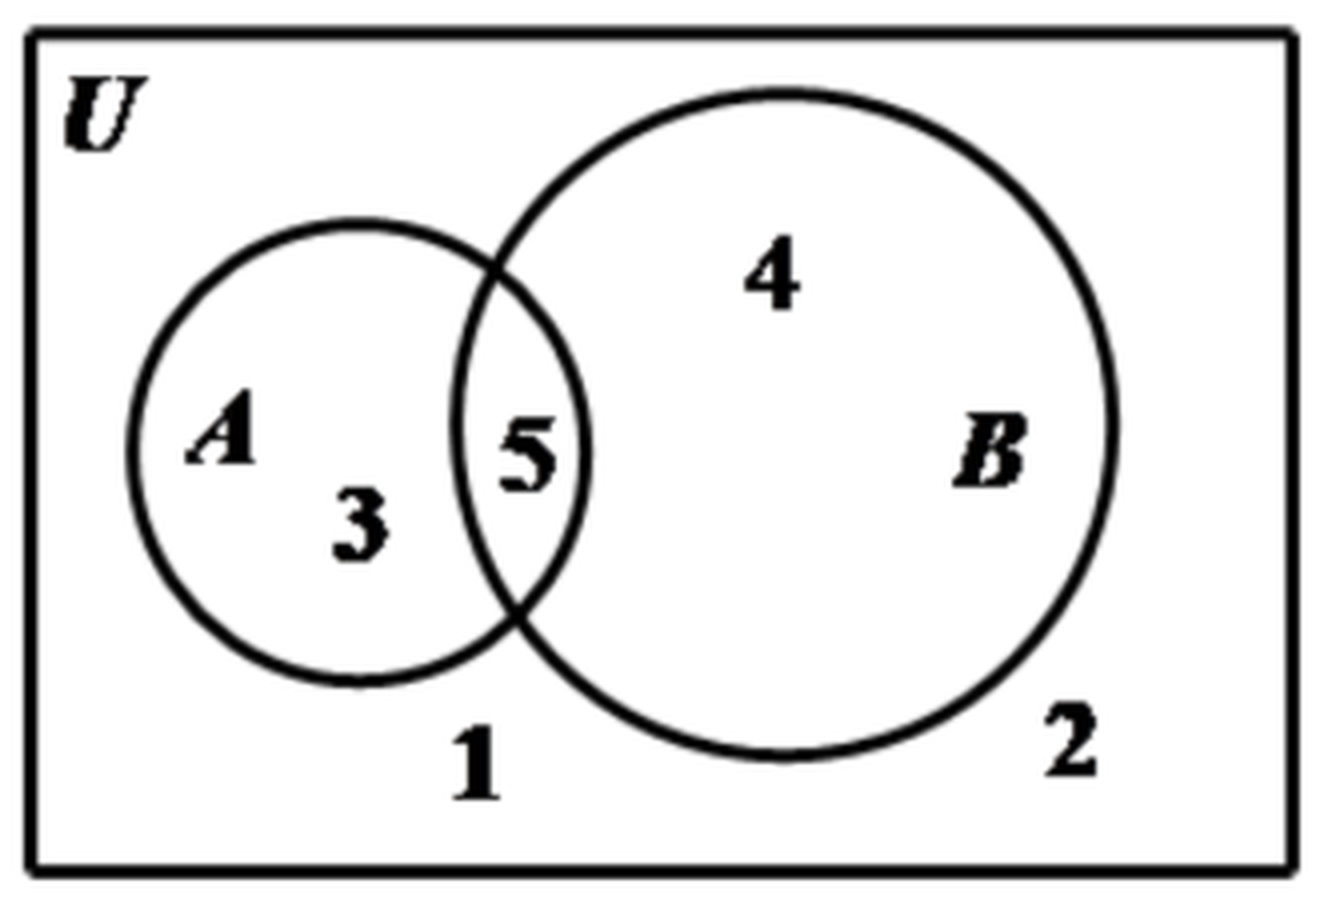
\includegraphics[width=0.28\textwidth]{figures/venn_U5_AB.png}
\end{center}

\keepwithprev
A. $3\notin A$ 且 $3\notin B$\qquad\qquad B. $3\in A$ 且 $3\in B$

C. $3\notin A$ 且 $3\in B$\qquad\qquad D. $3\in A$ 且 $3\notin B$

\ans{$D$}

\ifanswer
\solbegin
\step{画出韦恩图，得 $A=\{5,3\}$，$B=\{5,4\}$，}
\step{则 $3\in A$ 且 $3\notin B$. 故选 $D$.}
\solend

\fi

% 同第 13 题：整块（题干 + 图 + 选项）在答案版还要再挂【答案】【解析】，页末更易被拆开。
\needvspace{7.5cm}
\item 如图表示图形阴影部分的是\mbox{（\quad）}

\begin{center}
% 图取原卷截图、4× LANCZOS 放大（三圆 $A$、$B$、$C$，阴影为整个 $A$ 圆加 $B\cap C$）。
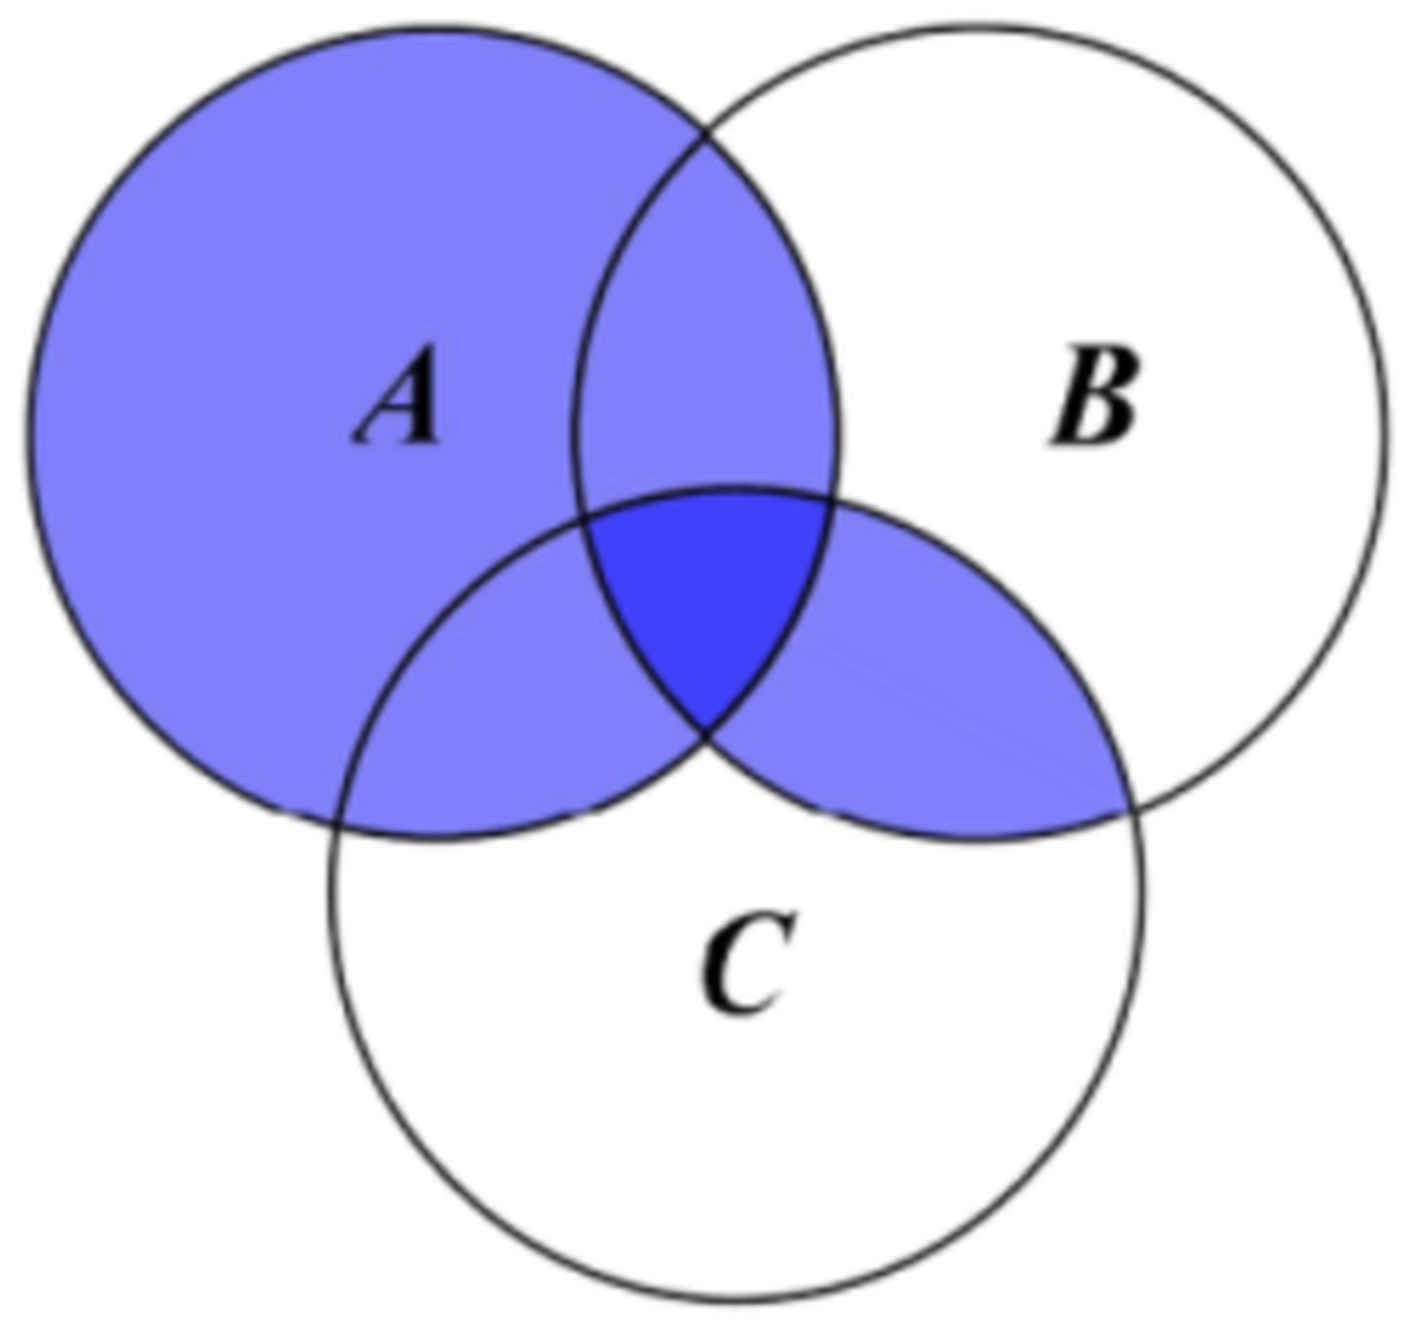
\includegraphics[width=0.30\textwidth]{figures/venn_A_union_BC.png}
\end{center}

\keepwithprev
A. $(A\cup C)\cap(B\cup C)$\qquad\qquad B. $(A\cup B)\cap(A\cup C)$

C. $(A\cup B)\cap(B\cup C)$\qquad\qquad D. $(A\cup B)\cap C$

\ans{$B$}

\ifanswer
\solbegin
\step{图中阴影部分表示元素满足是 $A$ 中的元素，或者是 $B$ 与 $C$ 的公共元素，}
\step{故可以表示为 $A\cup(B\cap C)$，也可以表示为 $(A\cup B)\cap(A\cup C)$.
故选 $B$.}
\solend

\fi

\item 设集合 $M=\left\{x\mid m\leqslant x\leqslant m+\dfrac34\right\}$，
$N=\left\{x\mid n-\dfrac13\leqslant x\leqslant n\right\}$，且 $M$、$N$ 都是集合
$\{x\mid0\leqslant x\leqslant1\}$ 的子集，如果把 $b-a$ 叫做集合
$\{x\mid a\leqslant x\leqslant b\}$ 的“长度”，那么集合 $M\cap N$ 的“长度”的
最小值是\mbox{（\quad）}

\keepwithprev
A. $\dfrac23$\qquad B. $\dfrac1{12}$\qquad C. $\dfrac13$\qquad D. $\dfrac5{12}$

\ans{$B$}

\ifanswer
\solbegin
\step{$M$ 的长度为 $\dfrac34$，$N$ 的长度为 $\dfrac13$，}
\step{当集合 $M\cap N$ 的长度的最小值时，$M$ 与 $N$ 应分别在区间 $[0,1]$ 的左右两端，}
\step{故 $M\cap N$ 的长度的最小值是 $\dfrac34+\dfrac13-1=\dfrac1{12}$，故选 $B$.}
\solend

\fi

\item 定义集合运算 $A-B=\{x\mid x\in A\text{ 且 }x\notin B\}$ 称为集合 $A$ 与集合 $B$ 的
差集；定义集合运算 $A\Delta B=(A-B)\cup(B-A)$ 称为集合 $A$ 与集合 $B$ 的对称差，
有以下 $4$ 个等式：① $A\Delta B=B\Delta A$；② $(A\Delta B)\Delta C=A\Delta(B\Delta C)$；
③ $A\cap(B\Delta C)=(A\cap B)\Delta(A\cap C)$；
④ $A\cup(B\Delta C)=(A\cup B)\Delta(A\cup C)$，
则 $4$ 个等式中恒成立的是\mbox{（\quad）}

\keepwithprev
A. ①②\qquad B. ①②③\qquad C. ①②④\qquad D. ①②③④

\ans{$B$}

\ifanswer
\solbegin
\step{对于①，由 $B\Delta A=(B-A)\cup(A-B)=(A-B)\cup(B-A)=A\Delta B$，
所以①正确；}
\step{对于②，由 $A-B=\{x\mid x\in A\text{ 且 }x\notin B\}
=\{x\mid x\in A,x\notin(A\cap B)\}=A-(A\cap B)$，}
\step{同理可得 $B-A=B-(A\cap B)$，}
\step{则 $A\Delta B=(A-B)\cup(B-A)=(A\cup B)-(A\cap B)$，}
\step{所以 $(A\Delta B)\Delta C=(A\Delta B)\cup C-(A\Delta B)\cap C$，}
\step{所以表示的集合为图（1）中阴影部分所表示的集合，如图所示，}
\step{同理 $A\Delta(B\Delta C)=A\cup(B\Delta C)-A\cap(B\Delta C)$，
也表示图（1）中阴影部分所表示的集合，}
\step{所以 $(A\Delta B)\Delta C=A\Delta(B\Delta C)$，所以②正确；}

\begin{center}
% 图取原卷截图、4× LANCZOS 放大（原卷印在下一页顶部，共三幅三圆韦恩图：
% 图（1）一幅、图（2）左右两幅，图（2）两幅下方各有一行式子标注）。
% 图只在【解析】里出现，故放进 \ifanswer 块，试卷版不排。
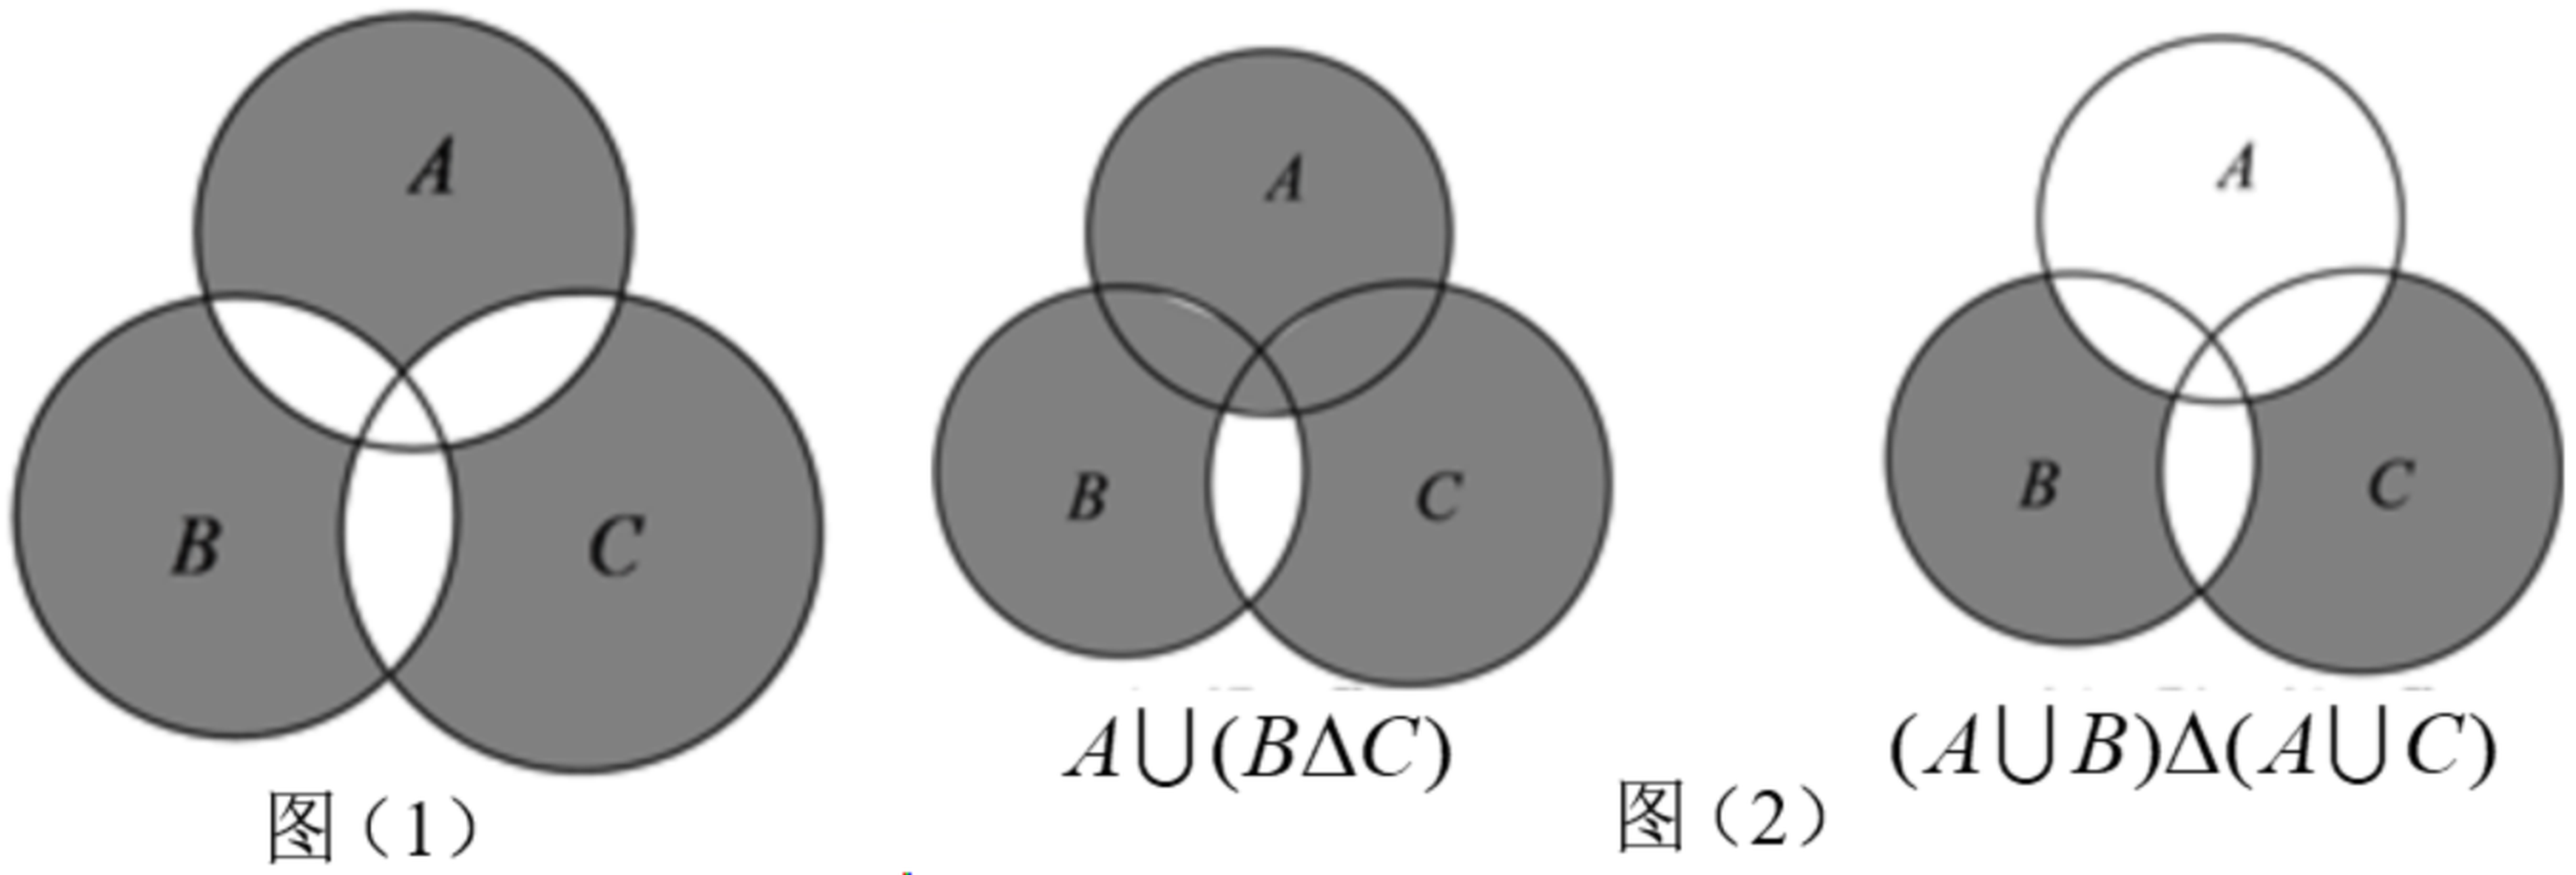
\includegraphics[width=0.86\textwidth]{figures/venn_symdiff3.png}
\end{center}

\step{对于③，由 $A\cap(B\Delta C)=A\cap(B\cup C-B\cap C)
=A\cap(B\cup C)-A\cap(B\cap C)$}
\step{$=(A\cap B)\cup(A\cap C)-(A\cap B)\cap(A\cap C)=(A\cap B)\Delta(A\cap C)$，
所以③正确；}
\step{对于④，如图（2）所示，$A\cup(B\Delta C)\neq(A\cup B)\Delta(A\cup C)$，
所以④错误.}
\step{故选 $B$.}
\solend

\fi

\end{enumerate}

\bigsec{三、解答题}

\begin{enumerate}
\setcounter{enumi}{16}

\item 已知集合 $M=\{x\mid a-1\leqslant x\leqslant2a+3\}$，$P=\{x\mid-2<x\leqslant4\}$，
全集 $U=\R$.

\begin{enumerate}[label=(\arabic*)]
\item 当 $a=2$ 时，求 $M\cap P$；
\item 若 $x\in P$ 是 $x\in M$ 的必要不充分条件，求实数 $a$ 的取值范围.
\end{enumerate}

\ifanswer
\solbegin
\stepm{(1)}{当 $a=2$ 时，集合 $M=\{x\mid1\leqslant x\leqslant7\}$，}
\step{所以 $M\cap P=\{x\mid1\leqslant x\leqslant4\}$；}
\stepm{(2)}{因为 $x\in P$ 是 $x\in M$ 的必要不充分条件，所以 $M\subset P$，}
\step{当 $M=\varnothing$ 时，$a-1>2a+3$，解得 $a<-4$，}
\step{当 $M\neq\varnothing$ 时，则
$\begin{cases}a-1\leqslant2a+3\\ a-1>-2\\ 2a+3\leqslant4\end{cases}$，
解得 $-1<a\leqslant\dfrac12$，}
\step{综上所述，实数 $a$ 的取值范围为
$(-\infty,-4)\cup\left(-1,\dfrac12\right]$.}
\solend

\fi

\ansspace[6]

\item 一辆汽车在某段路程中的行驶速度与时间的关系如图：

\begin{center}
% 图取原卷截图、4× LANCZOS 放大（速度—时间图：纵轴 $v/(\mathrm{km/h})$、
% 横轴 $t(\mathrm{h})$，$t\in[0,1]$、$[1,2]$、$[2,3]$ 三段矩形条高 50、80、90）。
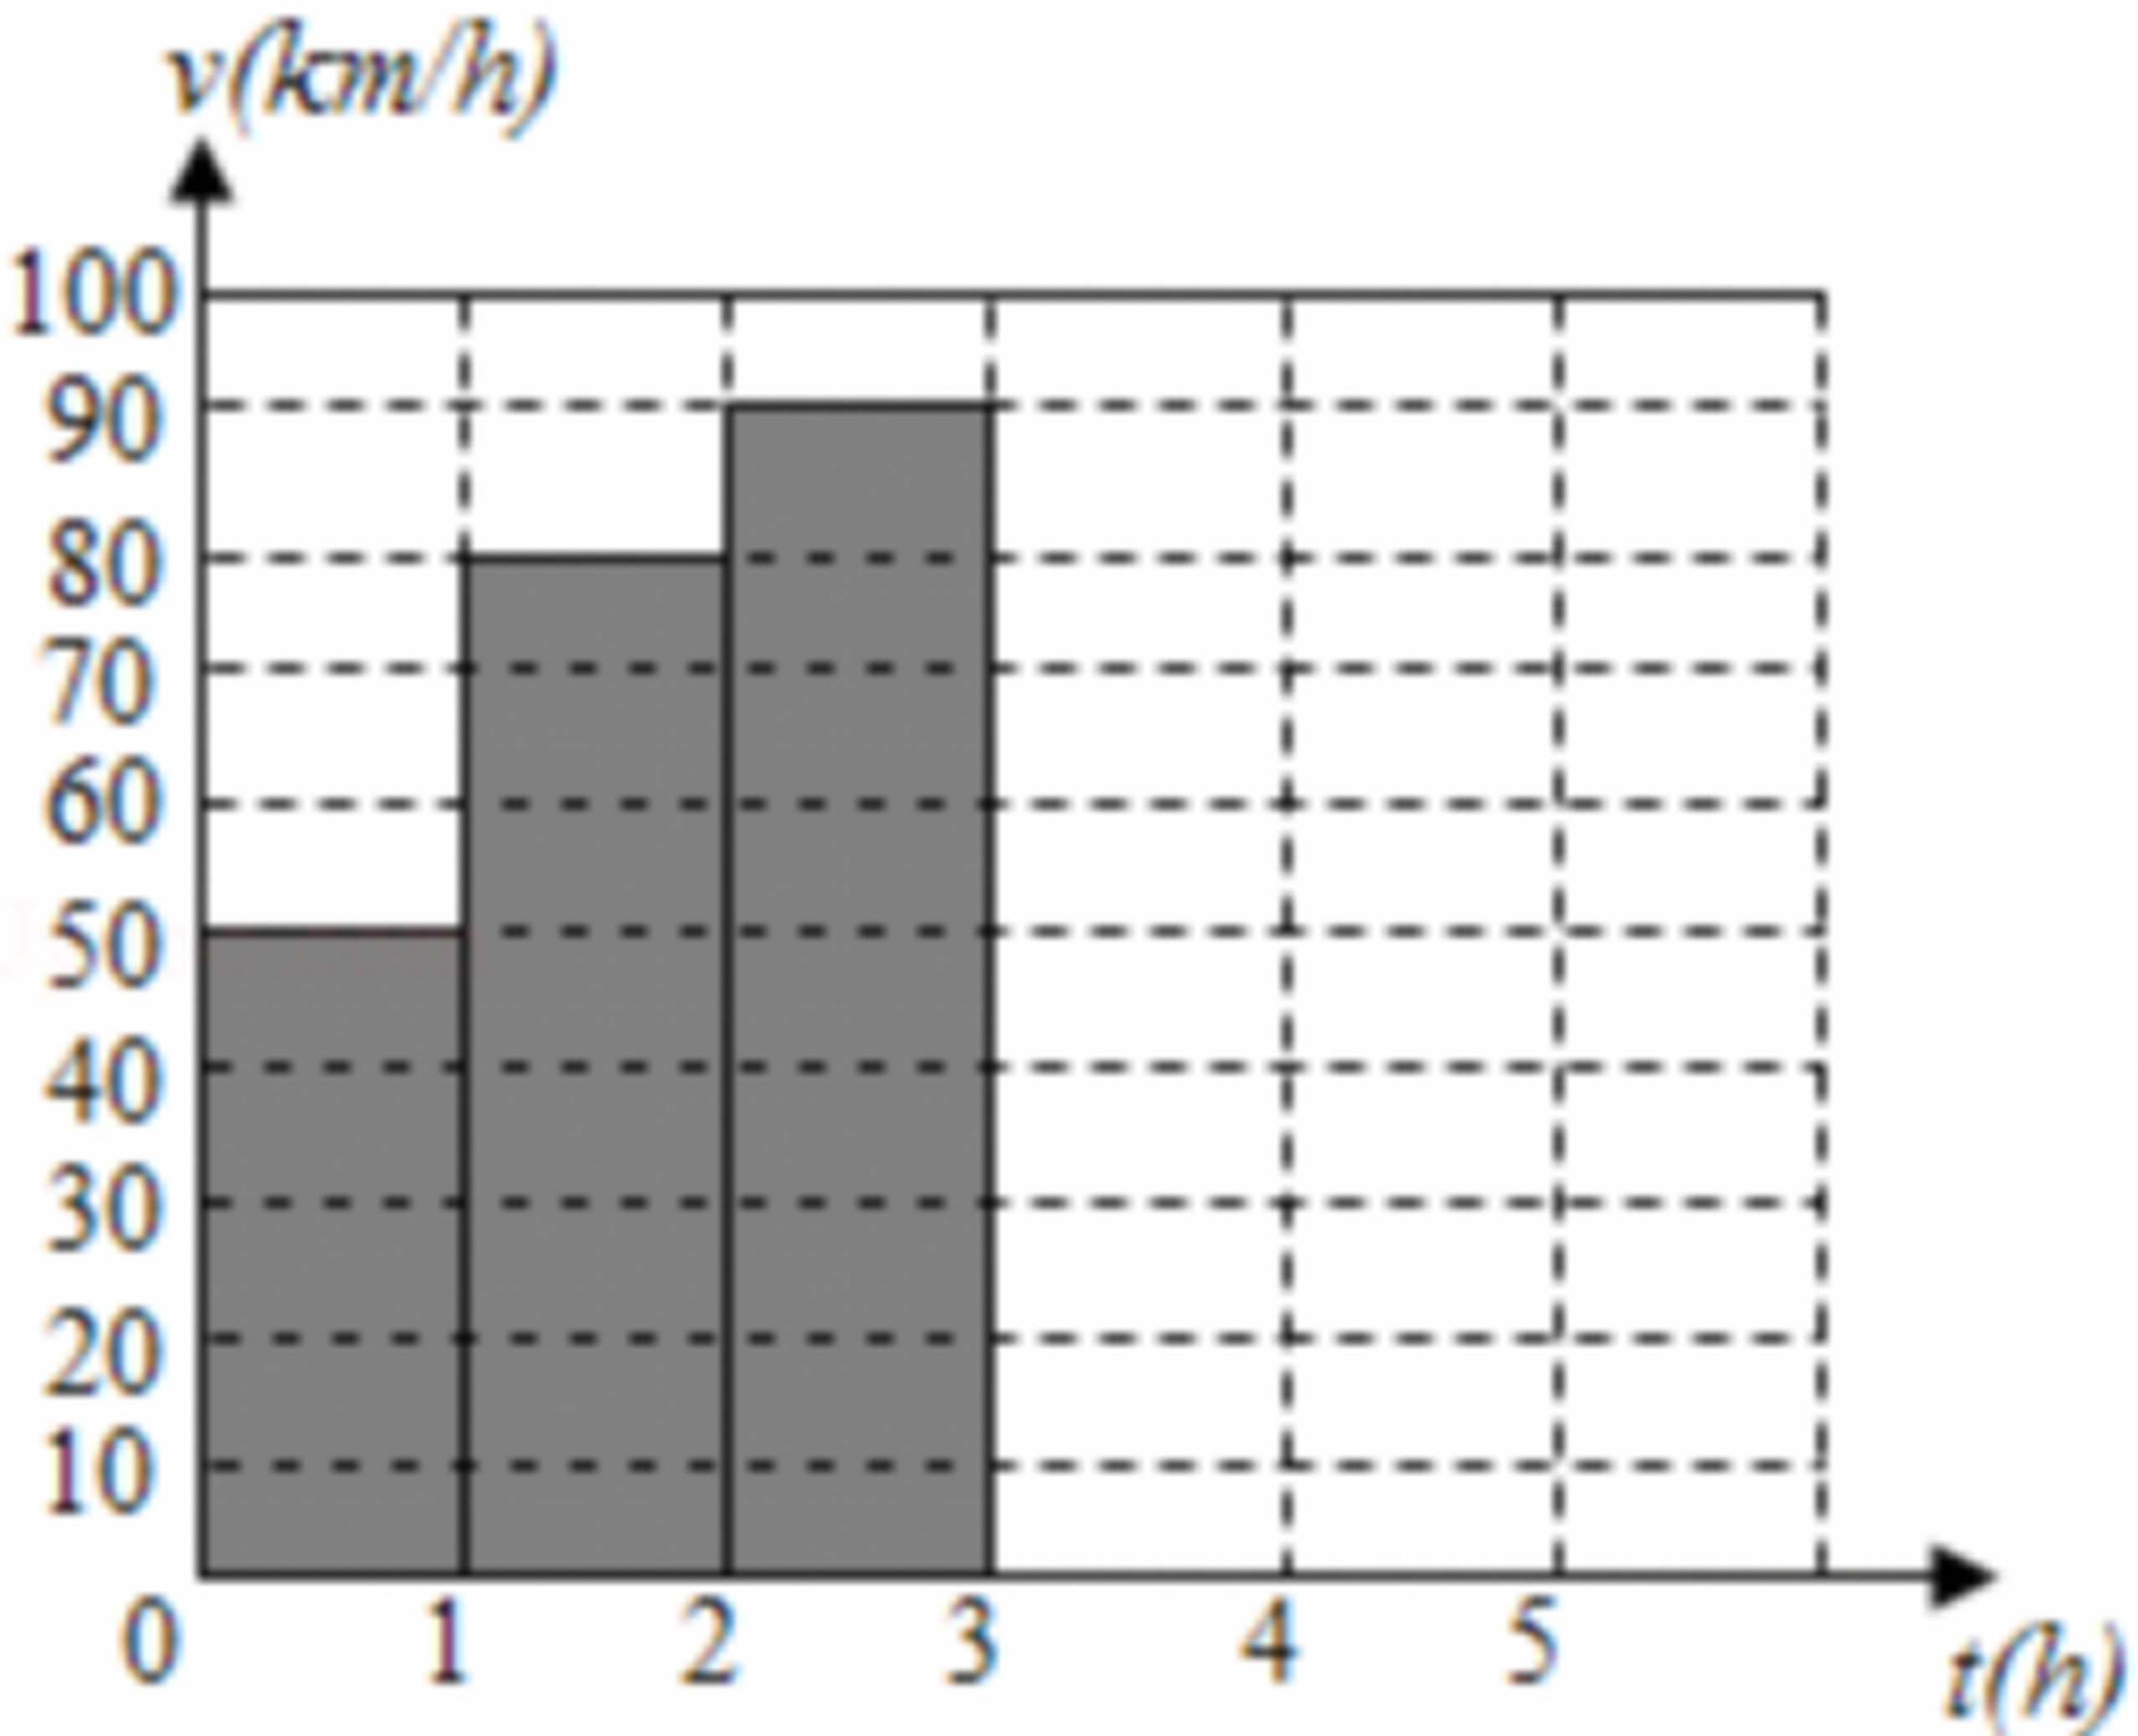
\includegraphics[width=0.52\textwidth]{figures/speed_time_bars.png}
\end{center}

\begin{enumerate}[label=(\arabic*)]
\item 求图中阴影部分的面积，并说明所求面积的实际意义；
\item 假设这辆汽车的里程表在汽车行驶这段路程前的读数为 $2004\,\mathrm{km}$，
试将汽车行驶这段路程时汽车里程表读数 $S$ 表示为时间 $t$ 的函数，
并求出当汽车里程表读数为 $2094\,\mathrm{km}$ 时，汽车行驶了多少时间？
\end{enumerate}

\ifanswer
\solbegin
\stepm{(1)}{由一辆汽车在某段路程中的行驶速度与时间的关系图，}
\step{得阴影部分的面积为 $50\times1+80\times1+90\times1=220$，}
\step{阴影部分的面积表示汽车在 $3$ 小时内行驶的路程为 $220\,\mathrm{km}$.}
\stepm{(2)}{$S=\begin{cases}
50t+2004,&0\leqslant t<1\\
80(t-1)+2054,&1\leqslant t<2\\
90(t-2)+2134,&2\leqslant t\leqslant3
\end{cases}$}
\step{令 $80(t-1)+2054=2094$，解得 $t=1.5$，所以汽车行驶 $1.5$ 小时.}
\solend

\fi

\ansspace[6]

\item 已知集合 $A=\{x\mid x<-2\text{ 或 }x\geqslant3\}$，$U=\R$.

\begin{enumerate}[label=(\arabic*)]
\item 求 $\overline{A}$；
\item 若 $B=\{x\mid mx-1>0\}$，当 $B\sub A$ 时，求实数 $m$ 的取值范围；
\item 若 $B=\{x\mid2m-6\leqslant x\leqslant m+4\}$，当 $B\cap\overline{A}=\varnothing$ 时，
求实数 $m$ 的取值范围.
\end{enumerate}

\ifanswer
\solbegin
\stepm{(1)}{因为集合 $A=\{x\mid x<-2\text{ 或 }x\geqslant3\}$，$U=\R$，
所以 $\overline{A}=\{x\mid-2\leqslant x<3\}$；}
\stepm{(2)}{当 $m=0$ 时，$B=\varnothing$，符合题意，}
\step{当 $m>0$ 时，$B=\left\{x\mid x>\dfrac1m\right\}$，则 $\dfrac1m\geqslant3$，
解得 $0<m\leqslant\dfrac13$，}
\step{当 $m<0$ 时，$B=\left\{x\mid x<\dfrac1m\right\}$，则 $\dfrac1m\leqslant-2$，
解得 $-\dfrac12\leqslant m<0$，}
\step{综上所述，实数 $m$ 的取值范围 $\left[-\dfrac12,\dfrac13\right]$；}
\stepm{(3)}{由题意得 $B=\{x\mid2m-6\leqslant x\leqslant m+4\}$，
$\overline{A}=\{x\mid-2\leqslant x<3\}$，且 $B\cap\overline{A}=\varnothing$，}
\step{当 $B=\varnothing$ 时，$2m-6>m+4$，解得 $m>10$，}
\step{当 $B\neq\varnothing$ 时，则 $\begin{cases}2m-6\leqslant m+4\\ m+4<-2\end{cases}$
或 $\begin{cases}2m-6\leqslant m+4\\ 2m-6\geqslant3\end{cases}$，}
\step{解得 $m<-6$ 或 $\dfrac92\leqslant m\leqslant10$，}
\step{综上所述，实数 $m$ 的取值范围为
$(-\infty,-6)\cup\left[\dfrac92,+\infty\right)$.}
\solend

\fi

\ansspace[8]

\item 在等腰梯形 $ABCD$ 中，$AB=DC=5$，$AD=4$，$BC=10$. 点 $E$ 在下底边 $BC$ 上.
点 $F$ 在腰 $AB$ 上.

\begin{center}
% 图取原卷截图、4× LANCZOS 放大（等腰梯形 $ABCD$ 与线段 $FE$，无辅助线）。
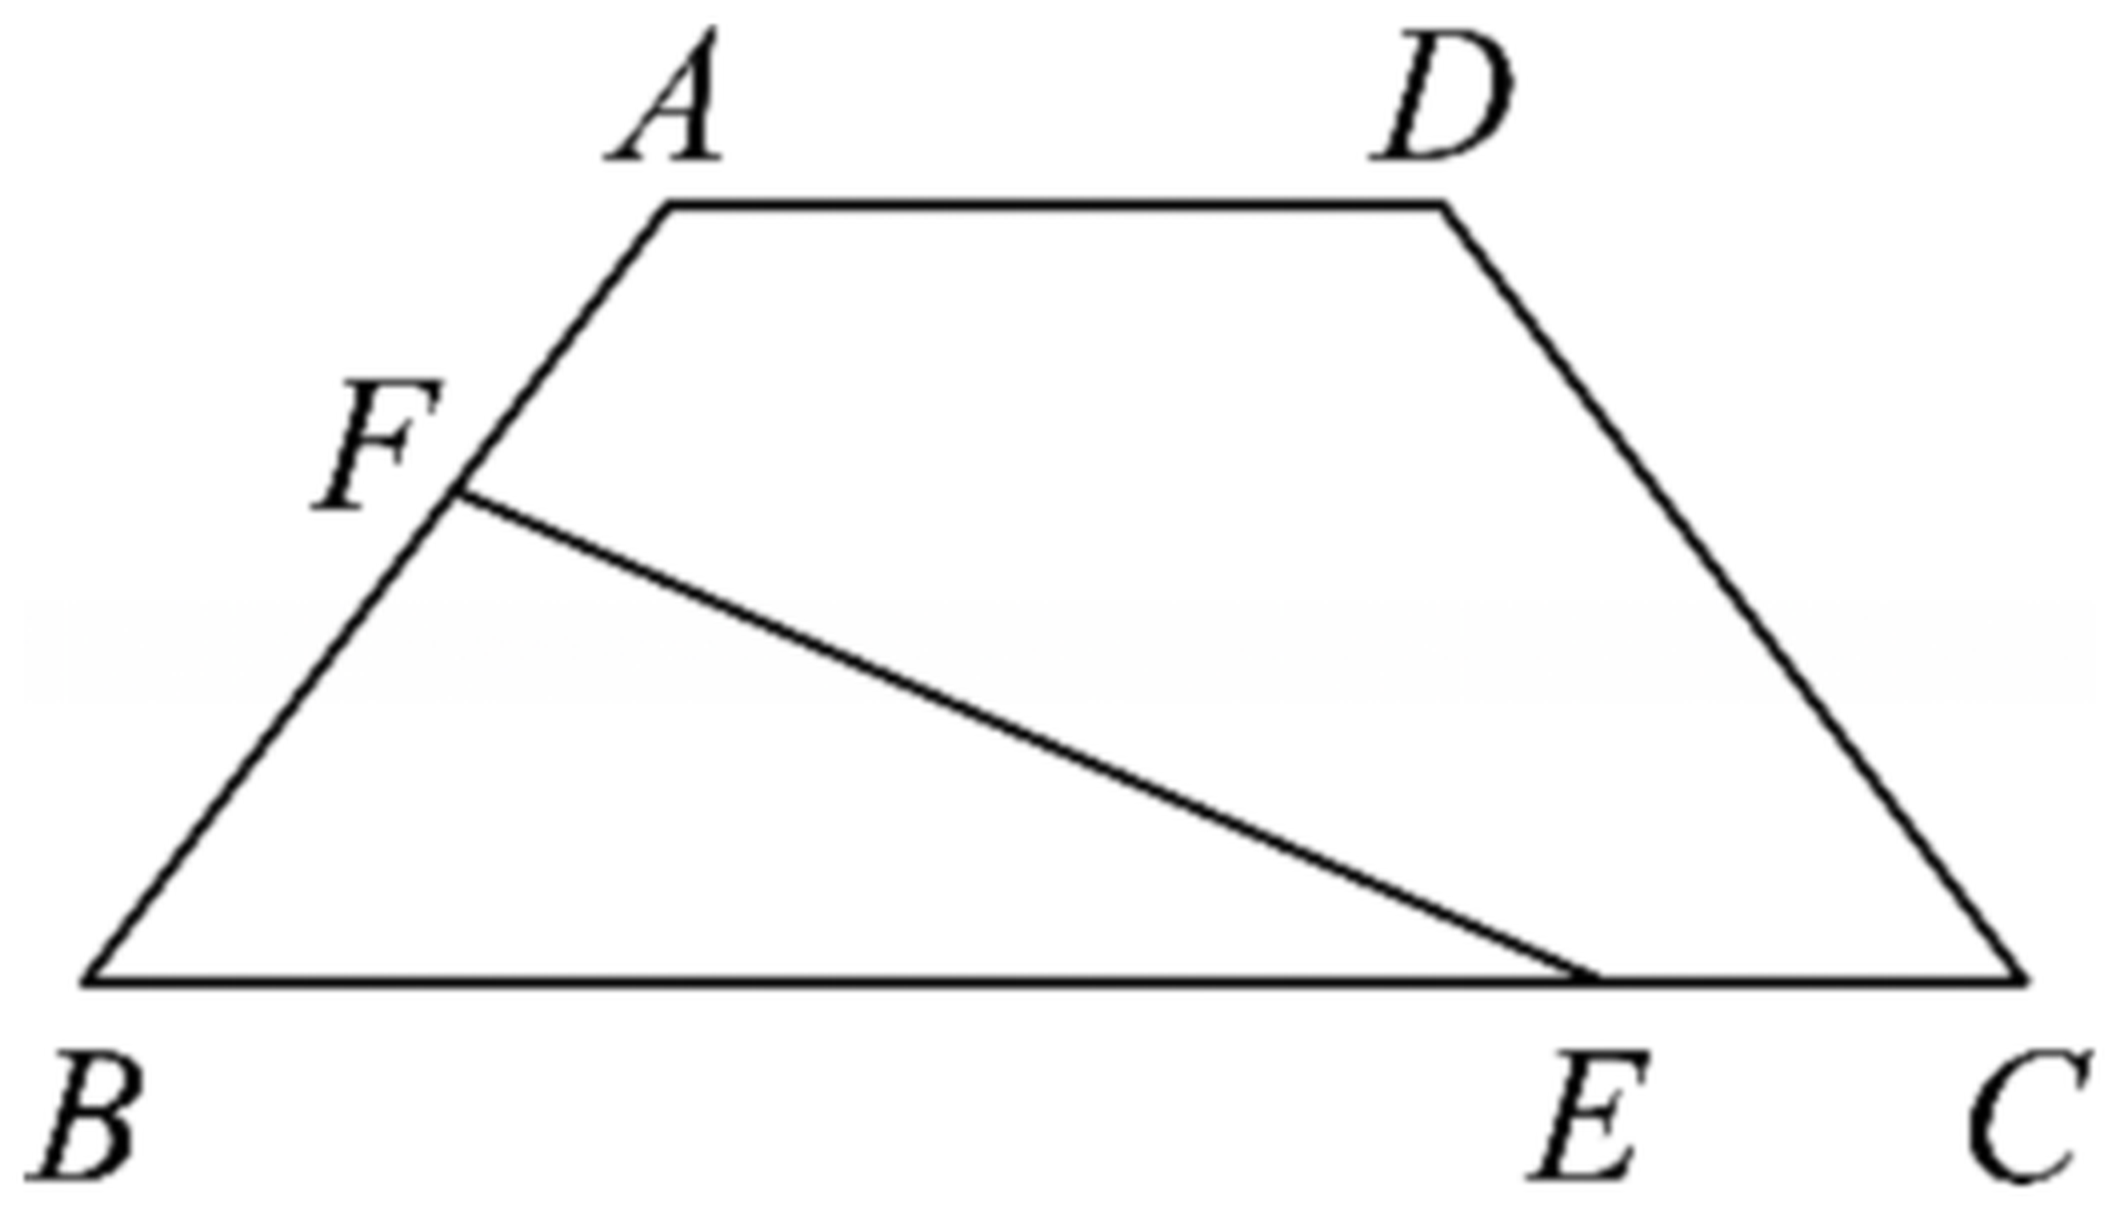
\includegraphics[width=0.46\textwidth]{figures/trapezoid_EF.png}
\end{center}

\begin{enumerate}[label=(\arabic*)]
\item 若 $EF$ 平分等腰梯形 $ABCD$ 的周长，设 $BE$ 长为 $x$，试用含 $x$ 的代数式表示
$\triangle BEF$ 的面积；
\item 是否存在线段 $EF$ 将等腰梯形 $ABCD$ 的周长和面积同时平分？若存在，求出此时 $BE$
的长；若不存在，请说明理由；
\item 是否存在线段 $EF$ 将等腰梯形 $ABCD$ 的周长和面积同时分成 $1:2$ 的两部分？
若存在，求此时 $BE$ 的长；若不存在，请说明理由.
\end{enumerate}

\ifanswer
\solbegin
\stepm{(1)}{过 $A$ 作 $AK\perp BC$ 交 $BC$ 于点 $K$，过 $F$ 作 $FG\perp BC$ 交 $BC$ 于点
$G$，}

\begin{center}
% 图取原卷截图、4× LANCZOS 放大（同梯形，多出虚线 $FG\perp BC$ 与 $AK\perp BC$
% 及两处直角符号；图只在【解析】里出现，故放进 \ifanswer 块）。
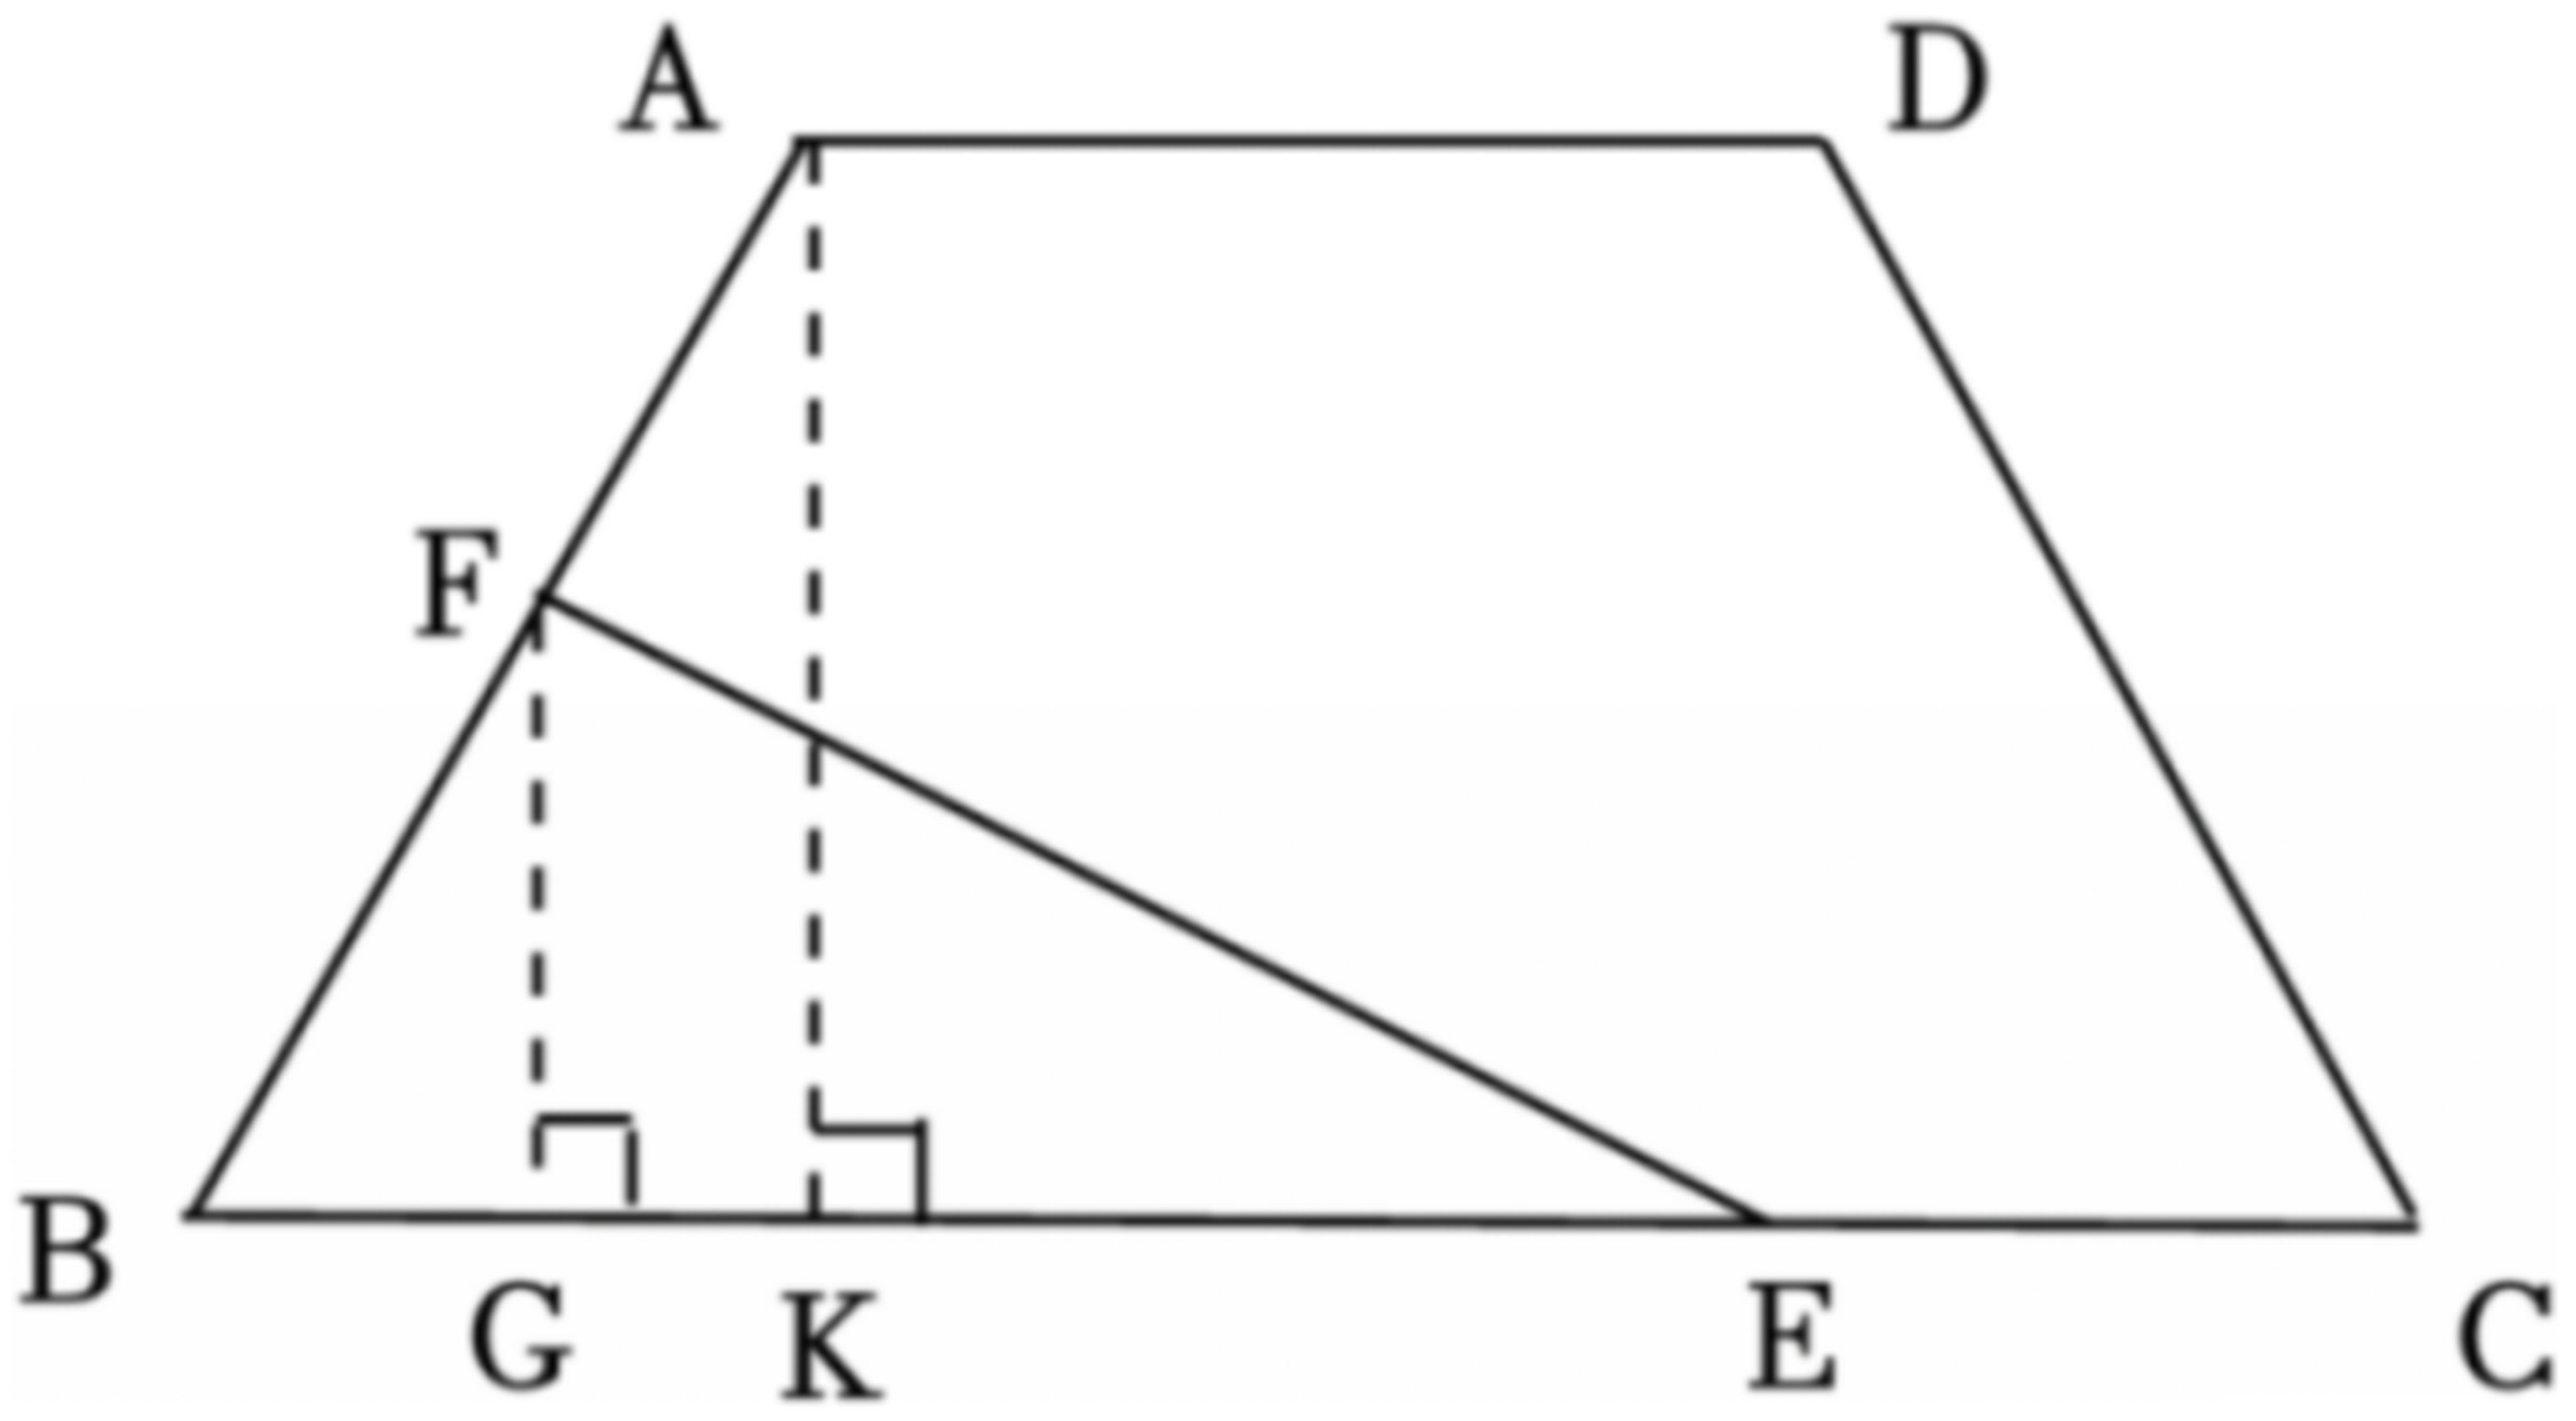
\includegraphics[width=0.62\textwidth]{figures/trapezoid_EF_aux.png}
\end{center}

\step{所以 $BK=\dfrac12\times(BC-AD)=\dfrac12\times(10-4)=3$，}
\step{$AK=\sqrt{AB^2-BK^2}=\sqrt{5^2-3^2}=4$，}
\step{由题意得，梯形 $ABCD$ 周长为 $24$，高为 $4$，面积为 $28$，}
\step{因为 $EF$ 平分等腰梯形 $ABCD$ 的周长，设 $BE$ 长为 $x$，则 $BF=12-x$，}
\step{由 $\begin{cases}0\leqslant12-x\leqslant5\\ 0\leqslant x\leqslant10\end{cases}$，
解得 $7\leqslant x\leqslant10$，}
\step{由题意得 $\triangle BFG\backsim\triangle BAK$，所以 $\dfrac{FG}{AK}=\dfrac{BF}{BA}$，
即 $\dfrac{FG}4=\dfrac{12-x}5$，}
\step{解得 $FG=\dfrac45(12-x)$，}
\step{所以 $S_{\triangle BEF}=\dfrac12BE\cdot FG
=-\dfrac25x^2+\dfrac{24}5x$（$7\leqslant x\leqslant10$）；}
\stepm{(2)}{存在，由 (1) 得 $-\dfrac25x^2+\dfrac{24}5x=\dfrac{28}2$，$x\in[7,10]$，}
\step{即 $x^2-12x+35=0$，解得 $x=7$ 或 $x=5$（舍去），}
\step{所以存在线段 $EF$ 将等腰梯形 $ABCD$ 的周长和面积同时平分，此时 $BE=7$；}
\stepm{(3)}{不存在，}
\step{情况一：$\triangle BEF$ 的面积$:$多边形 $AFECD$ 的面积 $=1:2$，
$(BE+BF):(AF+AD+DC+CE)=1:2$，}
\step{梯形周长的 $\dfrac13$ 是 $\dfrac{24}3=8$，面积的 $\dfrac13$ 是 $\dfrac{28}3$，}
\step{又因为 $BE=x$，所以 $BF=8-x$，}
\step{又因为 $\dfrac{FG}{AK}=\dfrac{BF}{BA}$，即 $\dfrac{FG}4=\dfrac{8-x}5$，
所以 $FG=\dfrac{32-4x}5$，}
\step{所以 $S_{\triangle BEF}=\dfrac12BE\times FG=-\dfrac25x^2+\dfrac{16}5x$，
所以 $\dfrac{28}3=-\dfrac25x^2+\dfrac{16}5x$，}
\step{整理得 $-3x^2+24x-70=0$，此时 $\Delta<0$，无解，故不存在；}
\step{情况二：$\triangle BEF$ 的面积$:$多边形 $AFECD$ 的面积 $=2:1$，
$(BE+BF):(AF+AD+DC+CE)=2:1$，}
\step{梯形周长的 $\dfrac13$ 为 $\dfrac{24}3=8$，面积的 $\dfrac13$ 为 $\dfrac{28}3$，
又 $BE=x$，所以 $BF=16-x$，}
\step{又 $\dfrac{FG}{AK}=\dfrac{BF}{BA}$，即 $\dfrac{FG}4=\dfrac{16-x}5$，
所以 $FG=\dfrac{64-4x}5$，}
\step{所以 $S_{\triangle BEF}=\dfrac12BE\times FG=-\dfrac25x^2+\dfrac{32}5x$，}
\step{所以 $\dfrac{28}3\times2=-\dfrac25x^2+\dfrac{32}5x$，
整理得 $-3x^2+48x-140=0$，}
\step{解得 $x=\dfrac{48+\sqrt{624}}6>10$，$x=\dfrac{48-\sqrt{624}}6<7$，
不符合题意，舍去，故不存在；}
\step{综上所述，不存在线段 $EF$ 将等腰梯形 $ABCD$ 的周长和面积同时分成 $1:2$ 的两部分.}
\solend

\fi

\ansspace[8]

\item 对集合 $\{1,2,\cdots,n\}$ 及其每一个非空子集 $A$，定义一个唯一确定的“交替和”
如下：将 $A$ 中的元素按照递减的次序排列，然后将第一个元素交替地减或加后继的元素所得的
结果，例如，子集 $\{1,2,4,6,9\}$ 的“交替和”是 $9-6+4-2+1=6$，子集 $\{5,6\}$ 的
“交替和”是 $6-5=1$，子集 $\{2\}$ 的交替和是 $2$；定义一个唯一确定的“交替积”如下：
将 $A$ 中的元素按照递减的次序排列，然后将第一个元素交替地除以或乘以后继的数所得的结果，
例如，集合 $\{1,2,4,6,9\}$ 的“交替积”是 $9\div6\times4\div2\times1=3$，
$\{5,6\}$ 的“交替积”是 $6\div5=1.2$，$\{2\}$ 的“交替积”是 $2$.

\begin{enumerate}[label=(\arabic*)]
\item 对于 $\{1,2,3,4,5,6,7,8,9\}$，求其所有子集的“交替和”的总和；
\item 对于 $\{1,2,\cdots,n\}$，求其所有子集的“交替和”的总和；
\item 对于 $\left\{n\mid\dfrac{495}{n+2}\in\N,n\in\Z\right\}$ 求其所有子集的
“交替积”的总和.
\end{enumerate}

\ifanswer
\solbegin
\stepm{(1)}{集合 $\{1,2,3,4,5,6,7,8,9\}$ 的子集中，除去 $\{9\}$ 外还有 $2^9-2$ 个
非空子集，}
\step{把这 $2^9-2$ 个非空子集两两组合后分别计算每一组中“交替和”之和，}
\step{组合原则是设 $A_i=\{9,a_1,a_2,\cdots\}$，$A_i^1=\{a_1,a_2,\cdots\}$，}
\step{集合 $A_i^1$ 的元素为集合 $A_i$ 中去掉 $9$ 的所有元素，把 $A_i$ 和 $A_i^1$
结合为一组，}
\step{显然，每组的“交替和”的和为 $9$，共有 $\dfrac{2^9-2}2$ 组，}
\step{所以，所有“交替和”之和应该为 $\dfrac{9(2^9-2)}2+9=2304$；}
\stepm{(2)}{集合 $\{1,2,\cdots,n\}$ 的子集中，除去 $\{n\}$ 外还有 $2^n-2$ 个非空子集，}
\step{把这 $2^n-2$ 个非空子集两两组合后分别计算每一组中“交替和”之和，}
\step{组合原则是设 $A_i=\{n,a_1,a_2,\cdots\}$，$A_i^1=\{a_1,a_2,\cdots\}$，}
\step{集合 $A_i^1$ 的元素为集合 $A_i$ 中去掉 $n$ 的所有元素，把 $A_i$ 和 $A_i^1$
结合为一组，}
\step{显然，每组的“交替和”的和为 $n$，共有 $\dfrac{2^n-2}2$ 组，}
% 注：下一行分子原卷印作花括号（其余同类处皆用圆括号），照抄未改，见文件头“原卷存疑”③。
\step{所以，所有“交替和”之和应该为 $\dfrac{n\{2^n-2\}}2+n=n\cdot2^{n-1}$；}
\stepm{(3)}{集合 $\left\{n\mid\dfrac{495}{n+2}\in\N,n\in\Z\right\}
=\{493,163,97,53,43,31,13,9,7,3,1,-1\}$，}
\step{其中除去 $\{-1\}$ 外还有 $2^{12}-2$ 个非空子集，}
% 注：下一行原卷把“把这”重复印了一次（“把这把这”），照抄未改，见文件头“原卷存疑”②。
\step{把这把这 $2^{12}-2$ 个非空子集两两组合后分别计算每一组中“交替积”之和，}
\step{组合原则是设 $A_j=\{-1,a_1,a_2,\cdots\}$，$A_j^1=\{a_1,a_2,\cdots\}$，}
\step{集合 $A_j^1$ 的元素为集合 $A_j$ 中去掉 $-1$ 的所有元素，把 $A_j$ 和 $A_j^1$
结合为一组，}
\step{显然，每组的“交替积”的和为 $0$，共有 $\dfrac{2^{12}-2}2$ 组，}
\step{所以，所有“交替积”之和应该为 $\dfrac{2^{12}-2}2\times0-1=-1$.}
\solend

\fi

\ansspace*[10]

\end{enumerate}

\end{document}
"
% 紧凑版：xelatex "\def\iscompact{1}% 高一30_南洋模范中学_开学考.tex
%   —— 高一上数学“2026-2027 年南洋模范中学高一上开学考”（试卷版/答案版）
% 试卷版：xelatex 高一30_南洋模范中学_开学考.tex
% 答案版：xelatex "\def\isanswer{1}\input{高一30_南洋模范中学_开学考.tex}"
% 紧凑版：xelatex "\def\iscompact{1}\input{高一30_南洋模范中学_开学考.tex}"
%
% 原始材料是微信公众号图文（公众号“魔都数学加油站”连载“27学年高一 30”，2026-09-23 发布，
% 原文标题“27学年高一30——2026-2027年上海市南洋模范中学高一上开学考”），
% 正文为 11 张 PNG 页。**同一篇里各页分辨率不一致**——第 2、3、9、10 页 4762×6735，
% 其余七页 2560×3620（已逐页打开确认，非下载缺档），取的是 mmbiz.qpic.cn/<hash>/0 的原图档。
% 原文本身就是一份**讲评版**：填空第 3—7 题下方印【答案】，第 8—12 题与其后各题印【解析】。
% 试题文字、答案与解析均照原卷录入，未改内容。卷面的粉色斜水印属水印，未录入。
%
% 卷首标题：原卷印作“2026-2027 年南洋模范中学高一上开学考”（公众号标题里的“上海市”
% 三字卷面标题行没有，本稿照卷面），年份区间按全稿惯例排 en dash，前缀照原卷保留“年”。
%
% 与原卷的排版差异（均已在 README“说明”中交代）：
%   ① 原文自**第 3 题**起（第 1、2 题未在该文中发布），故本稿题号亦自 3 起；
%   ② 原卷本就印有“一、填空题”“二、选择题”“三、解答题”三节标题，本稿照原卷分节，
%      只把标题改排成全稿统一的“大节标题”样式；
%   ③ 原卷填空第 3—7 题只印【答案】行、第 8 题起印【解析】（选择题答案写在解析末句
%      “故选 D／B”里），本稿统一改为试卷版隐去、答案版以 \ans{}／\ifanswer 块给出，
%      两版彻底分离；
%   ④ 子集符号原卷两种并用：第 7 题题干两处、第 19(2) 题作带下划线的 $\subseteq$，
%      第 17(2) 题解析作真包含的 $\subset$，本稿分别照录为 $\sub$ 与 $\subset$；
%   ⑤ 补集符号原卷一律作**上横线**（$\overline{A}$、$\overline{B}$），本稿照录；
%   ⑥ 原卷的实数集 R 一律作斜体（第 4 题、第 17 题与第 19 题题干的 $U=R$），
%      第 21(3) 题的自然数集与整数集作**粗体** $\mathbf{N}$、$\mathbf{Z}$，
%      本稿按全稿惯例统一写作 $\R$、$\N$、$\Z$；
%   ⑦ 原卷填空的横线约两个字宽，本稿按全稿惯例统一排 \blankline[4.4em]；
%   ⑧ 原卷未印副标题，本稿按全稿惯例补出副标题“集合与常用逻辑用语”——但本卷是开学考，
%      范围不止这一章：第 18 题是速度—时间图象题、第 20 题是等腰梯形的周长/面积平分问题，
%      副标题只标了主章节（见文末“高一30 专记”）；
%   ⑨ 第 13、14、18、20 题的图印在题干右侧、第 16 题的三幅图印在【解析】里的下一页顶部、
%      第 20 题【解析】另有一张带辅助线的图，本稿一律移至题干或解析之后；
%      图取原卷截图、4× LANCZOS 放大（见各 \includegraphics 前的注释）。
%
% 原卷存疑三处（均照抄原卷、未改，见源码中该处上方注释）：
%   ① 第 10 题【解析】验证“破晓集”时写的是 $\notin A$、$\in A$（如“$-2-2=-4\notin A$”），
%      但该处讨论的集合原题设里叫 $P$，同题②的“$x+y=2(k_1+k_2)\in A$”亦然——
%      本稿照抄未改（按文意应为 $P$）；
%   ② 第 21 题【解析】(3) 有“把这把这 $2^{12}-2$ 个非空子集”（“把这”重复印了一次）；
%   ③ 同题 (2) 的结论式分子原卷印作花括号 $\dfrac{n\{2^n-2\}}{2}$（其余同类处皆用圆括号）。

\documentclass[a4paper,11pt]{article}
\usepackage{common}

\begin{document}

\examtitlest[3]{2026--2027 年南洋模范中学高一上开学考}{集合与常用逻辑用语}

\bigsec{一、填空题}

\begin{enumerate}
\setcounter{enumi}{2}

\item 若集合 $A=\{x\mid x^2-2kx+7k=0\}$ 有且仅有三个真子集，则 $k$ 的取值范围是
\blankline[4.4em].

\ans{$(-\infty,0)\cup(7,+\infty)$}

\item “存在 $x\in\R$，使得 $x^2+2x+5=0$”的否定形式是 \blankline[4.4em].

\ans{对任何 $x\in\R$，都有 $x^2+2x+5\neq0$}

\item 下列命题中，$p$ 是 $q$ 的必要非充分条件的是 \blankline[4.4em].

① $p:x>2$ 且 $y>3$，$q:x+y>5$；

② $p$：四边形的四个角都相等，$q$：四边形是正方形.

\ans{②}

\item 若“条件 $\alpha:2\leqslant x\leqslant4$”是“条件 $\beta:3m-1\leqslant x\leqslant-m$”的
充分非必要条件，则 $m$ 的取值范围是 \blankline[4.4em].

\ans{$(-\infty,-4]$}

\item 满足 $\{1\}\sub M\sub\{1,2,4,5\}$ 的集合 $M$ 的个数为 \blankline[4.4em] 个.

\ans{$8$}

\item 已知集合 $A=\{1,2\}$，集合 $B=\{x\mid ax=6\}$，若 $A\cup B=A$，则 $a$ 的所有取值
构成的集合为 \blankline[4.4em].

\ifanswer
\solbegin
\step{因为 $A\cup B=A$，所以 $B\sub A$，}
\step{当 $a=0$ 时，$B=\varnothing$，满足 $B\sub A$；}
\step{当 $a\neq0$ 时，$B=\left\{\dfrac6a\right\}$，则 $\dfrac6a=1$ 或 $\dfrac6a=2$，
解得 $a=6$ 或 $a=3$，}
\step{综上所述，$a$ 的所有取值构成的集合为 $\{0,3,6\}$.}
\solend

\fi

\item 对于集合 $M$、$N$，定义 $M-N=\{x\mid x\in M\text{ 且 }x\notin N\}$，
$M\oplus N=(M-N)\cup(N-M)$，设 $A=\{y\mid y=|x|,x\in\R\}$，
$B=\{y\mid y=-(x-1)^2+2,x\in\R\}$，则 $A\oplus B=$ \blankline[4.4em].

\ifanswer
\solbegin
\step{由已知 $A=[0,+\infty)$，$B=(-\infty,2]$，}
\step{由于 $A-B=(2,+\infty)$，$B-A=(-\infty,0)$，}
\step{故 $A\oplus B=(A-B)\cup(B-A)=(-\infty,0)\cup(2,+\infty)$.}
\solend

\fi

\item 设 $P$ 为非空实数集满足：对任意给定的 $x$、$y\in P$（$x$、$y$ 可以相同），都有
$x+y\in P$，$x-y\in P$，$xy\in P$，则称 $P$ 为破晓集. 关于破晓集有下列结论：
①集合 $P=\{-2,-1,0,1,2\}$ 为破晓集；②集合 $P=\{x\mid x=2n,n\in\Z\}$ 为破晓集；
③若集合 $P_1$、$P_2$ 为破晓集，则 $P_1\cup P_2$ 为破晓集；④若集合 $P$ 为破晓集，
则一定有 $0\in P$；⑤若集合 $P_1$、$P_2$ 为破晓集，则 $P_1\cap P_2$ 为破晓集；
其中正确结论的序号是 \blankline[4.4em].

\ifanswer
\solbegin
% 注：以下几步原卷把该集合记作 $A$（题设里叫 $P$），照抄未改，见文件头“原卷存疑”①。
\step{对于①：$-2-2=-4\notin A$，故集合 $P=\{-2,-1,0,1,2\}$ 不为破晓集，故①错误；}
\step{②设 $x$、$y\in A$，则 $x=2k_1$，$y=2k_2$，且 $k_1$、$k_2\in\Z$，}
\step{故 $x+y=2(k_1+k_2)\in A$，$x-y=2(k_1-k_2)\in A$，$xy=4k_1k_2\in A$，}
\step{故集合 $P=\{x\mid x=2n,n\in\Z\}$ 为破晓集，故②正确；}
\step{③若集合 $P_1$、$P_2$ 为破晓集，设 $P_1=\{x\mid x=2k,k\in\Z\}$，
$P_2=\{x\mid x=3k,k\in\Z\}$，}
\step{但是 $P_1\cup P_2$ 不为破晓集，如 $x=2$，$y=3$ 时，$x+y=5$，
故 $5\notin(P_1\cup P_2)$，故③错误；}
\step{④若集合 $P$ 为破晓集，则取 $x=y$，$x-y=0\in A$，则一定有 $0\in P$，故④正确.}
\step{⑤正确；}
\step{故正确的是②④⑤.}
\solend

\fi

\item 已知集合 $M$ 的元素均为正整数，定义集合 $M$ 的“变项和”为：将 $M$ 中每个元素 $m$
都乘以 $(-1)^m$ 后再求和. 若集合 $A=\{n\mid1\leqslant n\leqslant10,n\in\N\}$，则集合 $A$
的所有非空子集的“变项和”的总和为 \blankline[4.4em].

\ifanswer
\solbegin
\step{$A$ 集合的所有非空子集中，每个元素出现的次数都是
$(2^{10}-1)-(2^9-1)=2^9$，}
\step{则集合 $A$ 的所有非空子集的“变项和”的总和为
$1\times(-1)^1\times2^9+2\times(-1)^2\times2^9+\cdots+10\times(-1)^{10}\times2^9$}
\step{$=(-1+2-3+4-\cdots-9+10)\times2^9=5\times2^9=2560$.}
\solend

\fi

\item 已知集合 $A=[t,t+1]\cup[t+4,t+9]$，$0\notin A$，存在正数 $\lambda$，使得对任意
$a\in A$，都有 $\dfrac\lambda a\in A$，则 $t$ 的值是 \blankline[4.4em].

\ifanswer
\solbegin
\step{当 $t>0$ 时，当 $a\in[t,t+1]$ 时，$\dfrac\lambda a\in[t+4,t+9]$，}
\step{当 $a\in[t+4,t+9]$ 时，$\dfrac\lambda a\in[t,t+1]$，}
\step{即当 $a=t$ 时，$\dfrac\lambda a\leqslant t+9$；当 $a=t+9$ 时，
$\dfrac\lambda a\geqslant t$，即 $\lambda=t(t+9)$；}
\step{当 $a=t+1$ 时，$\dfrac\lambda a\geqslant t+4$，当 $a=t+4$ 时，
$\dfrac\lambda a\leqslant t+1$，即 $\lambda=(t+1)(t+4)$，}
\step{所以 $t(t+9)=(t+1)(t+4)$，解得 $t=1$.}
\step{当 $t+1<0<t+4$ 时，当 $a\in[t,t+1]$ 时，$\dfrac\lambda a\in[t,t+1]$.}
\step{当 $a\in[t+4,t+9]$ 时，则 $\dfrac\lambda a\in[t+4,t+9]$，}
\step{即当 $a=t$ 时，$\dfrac\lambda a\leqslant t+1$，当 $a=t+1$ 时，
$\dfrac\lambda a\geqslant t$，即 $\lambda=t(t+1)$，}
\step{即当 $a=t+4$ 时，$\dfrac\lambda a\leqslant t+9$，当 $a=t+9$ 时，
$\dfrac\lambda a\geqslant t+4$，即 $\lambda=(t+4)(t+9)$，}
\step{所以 $t(t+1)=(t+4)(t+9)$，解得 $t=-3$.}
\step{当 $t+9<0$ 时，同理可得无解.}
\step{综上，$t$ 的值为 $1$ 或 $-3$.}
\solend

\fi

\end{enumerate}

\bigsec{二、选择题}

\begin{enumerate}
\setcounter{enumi}{12}

% 这道题是“题干 + 图 + 选项”约 6cm 的一整块，页末放不下就会被拆开（切页审计的 A 类），
% 故在题前先量一次页高：不够就把整道题干连图带选项一起挪到次页。
\needvspace{6.5cm}
\item 设 $U=\{1,2,3,4,5\}$，$A$、$B$ 都是 $U$ 的子集，且 $A\cap B=\{5\}$，
$\overline{A}\cap B=\{4\}$，$\overline{A}\cap\overline{B}=\{1,2\}$，
则以下四个判断中正确的是\mbox{（\quad）}

\begin{center}
% 图取原卷截图、4× LANCZOS 放大（原卷把图印在题干右侧，本稿移至此处，见文件头⑨）。
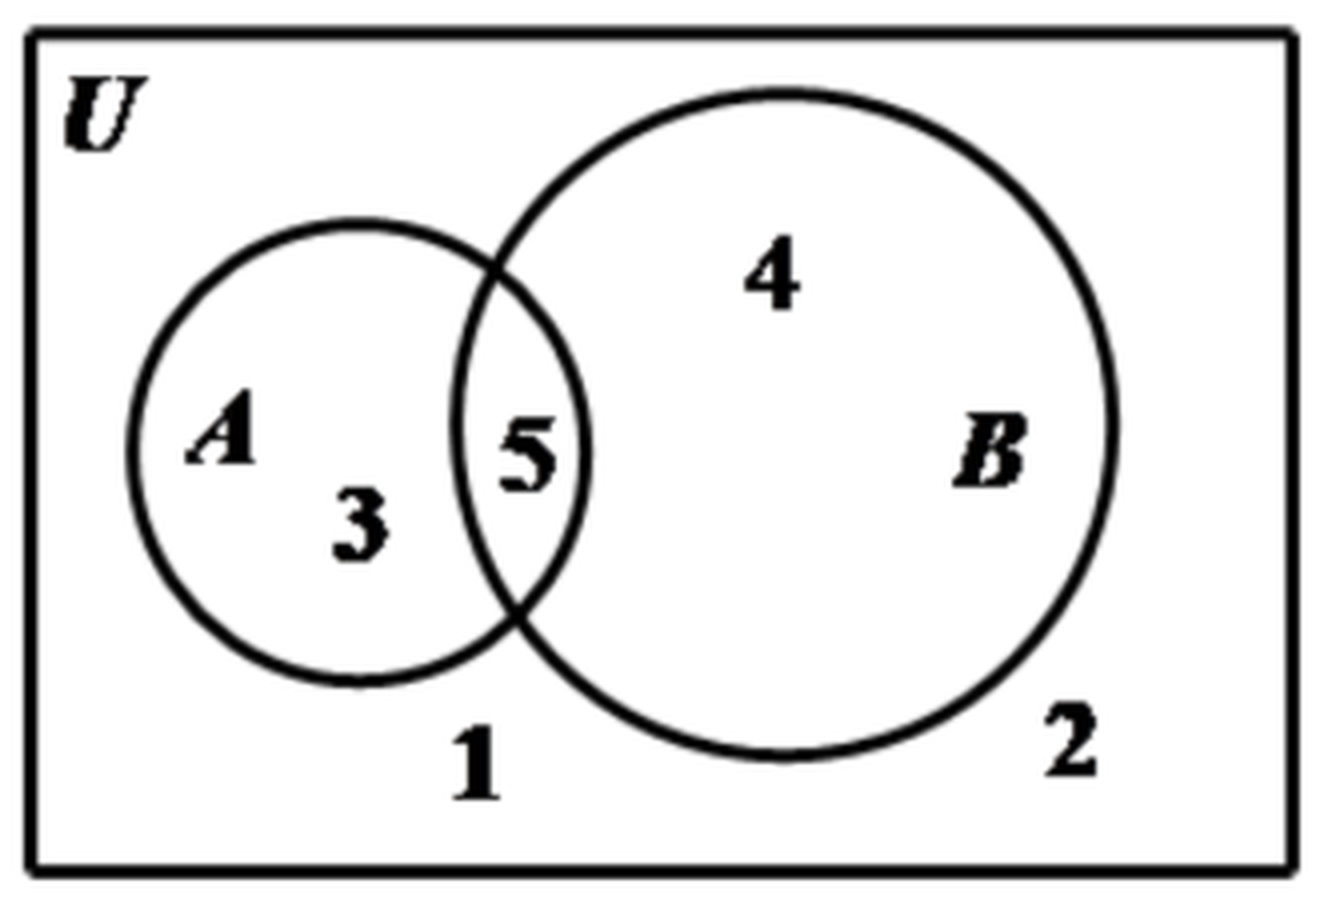
\includegraphics[width=0.28\textwidth]{figures/venn_U5_AB.png}
\end{center}

\keepwithprev
A. $3\notin A$ 且 $3\notin B$\qquad\qquad B. $3\in A$ 且 $3\in B$

C. $3\notin A$ 且 $3\in B$\qquad\qquad D. $3\in A$ 且 $3\notin B$

\ans{$D$}

\ifanswer
\solbegin
\step{画出韦恩图，得 $A=\{5,3\}$，$B=\{5,4\}$，}
\step{则 $3\in A$ 且 $3\notin B$. 故选 $D$.}
\solend

\fi

% 同第 13 题：整块（题干 + 图 + 选项）在答案版还要再挂【答案】【解析】，页末更易被拆开。
\needvspace{7.5cm}
\item 如图表示图形阴影部分的是\mbox{（\quad）}

\begin{center}
% 图取原卷截图、4× LANCZOS 放大（三圆 $A$、$B$、$C$，阴影为整个 $A$ 圆加 $B\cap C$）。
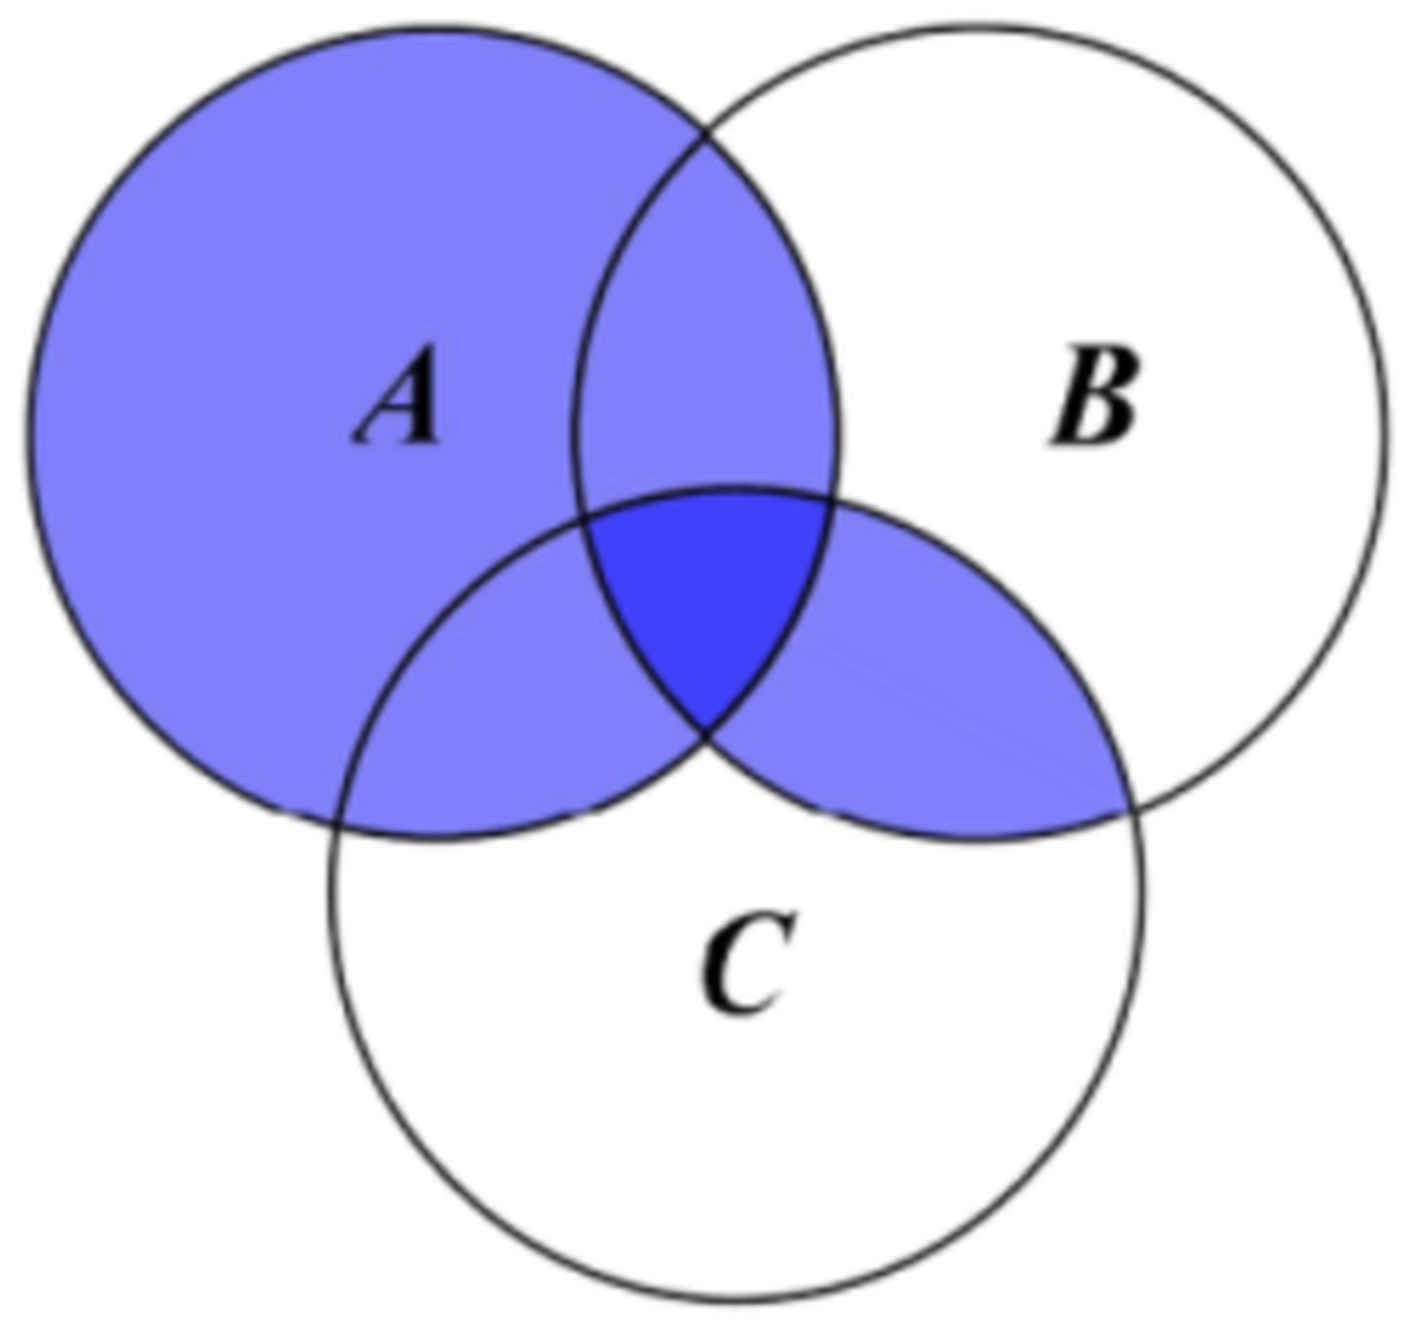
\includegraphics[width=0.30\textwidth]{figures/venn_A_union_BC.png}
\end{center}

\keepwithprev
A. $(A\cup C)\cap(B\cup C)$\qquad\qquad B. $(A\cup B)\cap(A\cup C)$

C. $(A\cup B)\cap(B\cup C)$\qquad\qquad D. $(A\cup B)\cap C$

\ans{$B$}

\ifanswer
\solbegin
\step{图中阴影部分表示元素满足是 $A$ 中的元素，或者是 $B$ 与 $C$ 的公共元素，}
\step{故可以表示为 $A\cup(B\cap C)$，也可以表示为 $(A\cup B)\cap(A\cup C)$.
故选 $B$.}
\solend

\fi

\item 设集合 $M=\left\{x\mid m\leqslant x\leqslant m+\dfrac34\right\}$，
$N=\left\{x\mid n-\dfrac13\leqslant x\leqslant n\right\}$，且 $M$、$N$ 都是集合
$\{x\mid0\leqslant x\leqslant1\}$ 的子集，如果把 $b-a$ 叫做集合
$\{x\mid a\leqslant x\leqslant b\}$ 的“长度”，那么集合 $M\cap N$ 的“长度”的
最小值是\mbox{（\quad）}

\keepwithprev
A. $\dfrac23$\qquad B. $\dfrac1{12}$\qquad C. $\dfrac13$\qquad D. $\dfrac5{12}$

\ans{$B$}

\ifanswer
\solbegin
\step{$M$ 的长度为 $\dfrac34$，$N$ 的长度为 $\dfrac13$，}
\step{当集合 $M\cap N$ 的长度的最小值时，$M$ 与 $N$ 应分别在区间 $[0,1]$ 的左右两端，}
\step{故 $M\cap N$ 的长度的最小值是 $\dfrac34+\dfrac13-1=\dfrac1{12}$，故选 $B$.}
\solend

\fi

\item 定义集合运算 $A-B=\{x\mid x\in A\text{ 且 }x\notin B\}$ 称为集合 $A$ 与集合 $B$ 的
差集；定义集合运算 $A\Delta B=(A-B)\cup(B-A)$ 称为集合 $A$ 与集合 $B$ 的对称差，
有以下 $4$ 个等式：① $A\Delta B=B\Delta A$；② $(A\Delta B)\Delta C=A\Delta(B\Delta C)$；
③ $A\cap(B\Delta C)=(A\cap B)\Delta(A\cap C)$；
④ $A\cup(B\Delta C)=(A\cup B)\Delta(A\cup C)$，
则 $4$ 个等式中恒成立的是\mbox{（\quad）}

\keepwithprev
A. ①②\qquad B. ①②③\qquad C. ①②④\qquad D. ①②③④

\ans{$B$}

\ifanswer
\solbegin
\step{对于①，由 $B\Delta A=(B-A)\cup(A-B)=(A-B)\cup(B-A)=A\Delta B$，
所以①正确；}
\step{对于②，由 $A-B=\{x\mid x\in A\text{ 且 }x\notin B\}
=\{x\mid x\in A,x\notin(A\cap B)\}=A-(A\cap B)$，}
\step{同理可得 $B-A=B-(A\cap B)$，}
\step{则 $A\Delta B=(A-B)\cup(B-A)=(A\cup B)-(A\cap B)$，}
\step{所以 $(A\Delta B)\Delta C=(A\Delta B)\cup C-(A\Delta B)\cap C$，}
\step{所以表示的集合为图（1）中阴影部分所表示的集合，如图所示，}
\step{同理 $A\Delta(B\Delta C)=A\cup(B\Delta C)-A\cap(B\Delta C)$，
也表示图（1）中阴影部分所表示的集合，}
\step{所以 $(A\Delta B)\Delta C=A\Delta(B\Delta C)$，所以②正确；}

\begin{center}
% 图取原卷截图、4× LANCZOS 放大（原卷印在下一页顶部，共三幅三圆韦恩图：
% 图（1）一幅、图（2）左右两幅，图（2）两幅下方各有一行式子标注）。
% 图只在【解析】里出现，故放进 \ifanswer 块，试卷版不排。
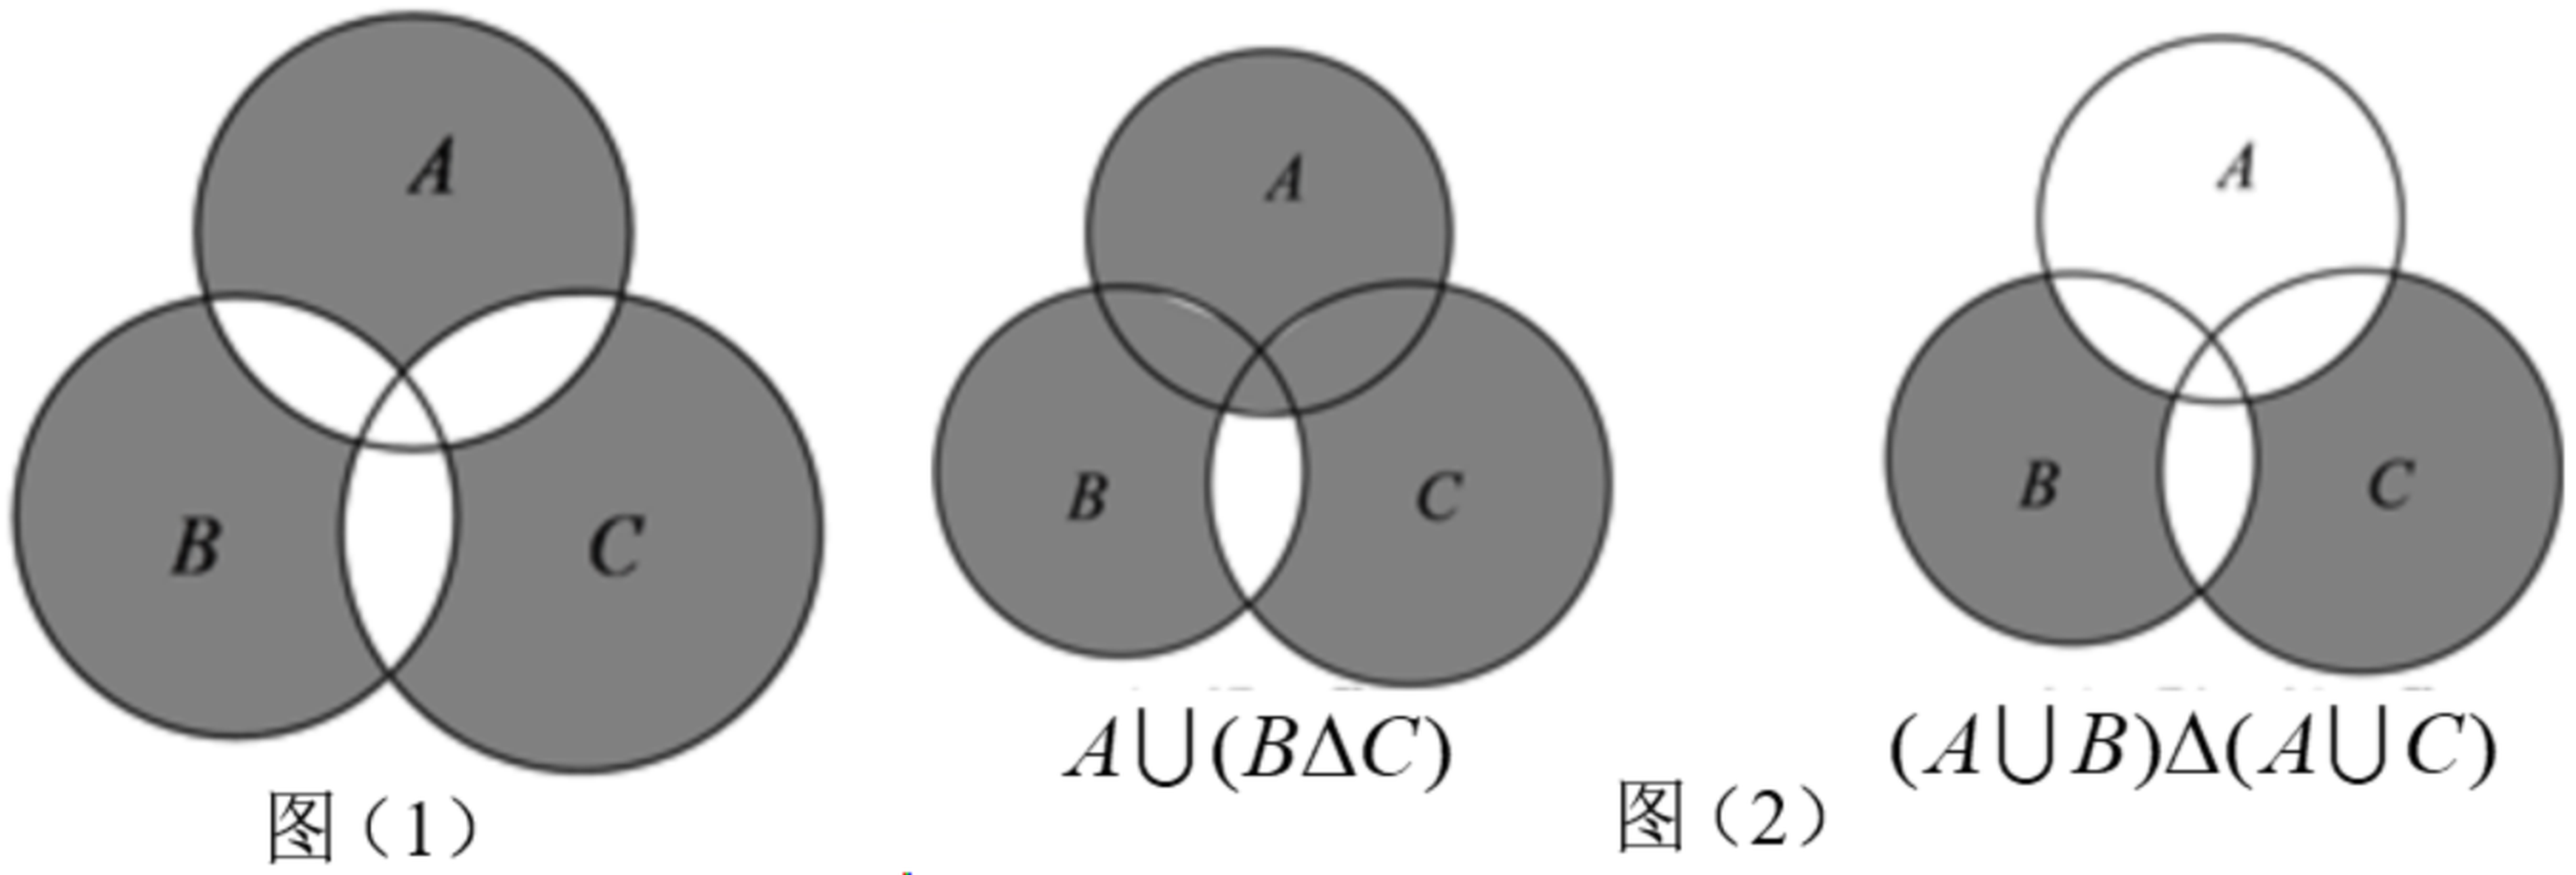
\includegraphics[width=0.86\textwidth]{figures/venn_symdiff3.png}
\end{center}

\step{对于③，由 $A\cap(B\Delta C)=A\cap(B\cup C-B\cap C)
=A\cap(B\cup C)-A\cap(B\cap C)$}
\step{$=(A\cap B)\cup(A\cap C)-(A\cap B)\cap(A\cap C)=(A\cap B)\Delta(A\cap C)$，
所以③正确；}
\step{对于④，如图（2）所示，$A\cup(B\Delta C)\neq(A\cup B)\Delta(A\cup C)$，
所以④错误.}
\step{故选 $B$.}
\solend

\fi

\end{enumerate}

\bigsec{三、解答题}

\begin{enumerate}
\setcounter{enumi}{16}

\item 已知集合 $M=\{x\mid a-1\leqslant x\leqslant2a+3\}$，$P=\{x\mid-2<x\leqslant4\}$，
全集 $U=\R$.

\begin{enumerate}[label=(\arabic*)]
\item 当 $a=2$ 时，求 $M\cap P$；
\item 若 $x\in P$ 是 $x\in M$ 的必要不充分条件，求实数 $a$ 的取值范围.
\end{enumerate}

\ifanswer
\solbegin
\stepm{(1)}{当 $a=2$ 时，集合 $M=\{x\mid1\leqslant x\leqslant7\}$，}
\step{所以 $M\cap P=\{x\mid1\leqslant x\leqslant4\}$；}
\stepm{(2)}{因为 $x\in P$ 是 $x\in M$ 的必要不充分条件，所以 $M\subset P$，}
\step{当 $M=\varnothing$ 时，$a-1>2a+3$，解得 $a<-4$，}
\step{当 $M\neq\varnothing$ 时，则
$\begin{cases}a-1\leqslant2a+3\\ a-1>-2\\ 2a+3\leqslant4\end{cases}$，
解得 $-1<a\leqslant\dfrac12$，}
\step{综上所述，实数 $a$ 的取值范围为
$(-\infty,-4)\cup\left(-1,\dfrac12\right]$.}
\solend

\fi

\ansspace[6]

\item 一辆汽车在某段路程中的行驶速度与时间的关系如图：

\begin{center}
% 图取原卷截图、4× LANCZOS 放大（速度—时间图：纵轴 $v/(\mathrm{km/h})$、
% 横轴 $t(\mathrm{h})$，$t\in[0,1]$、$[1,2]$、$[2,3]$ 三段矩形条高 50、80、90）。
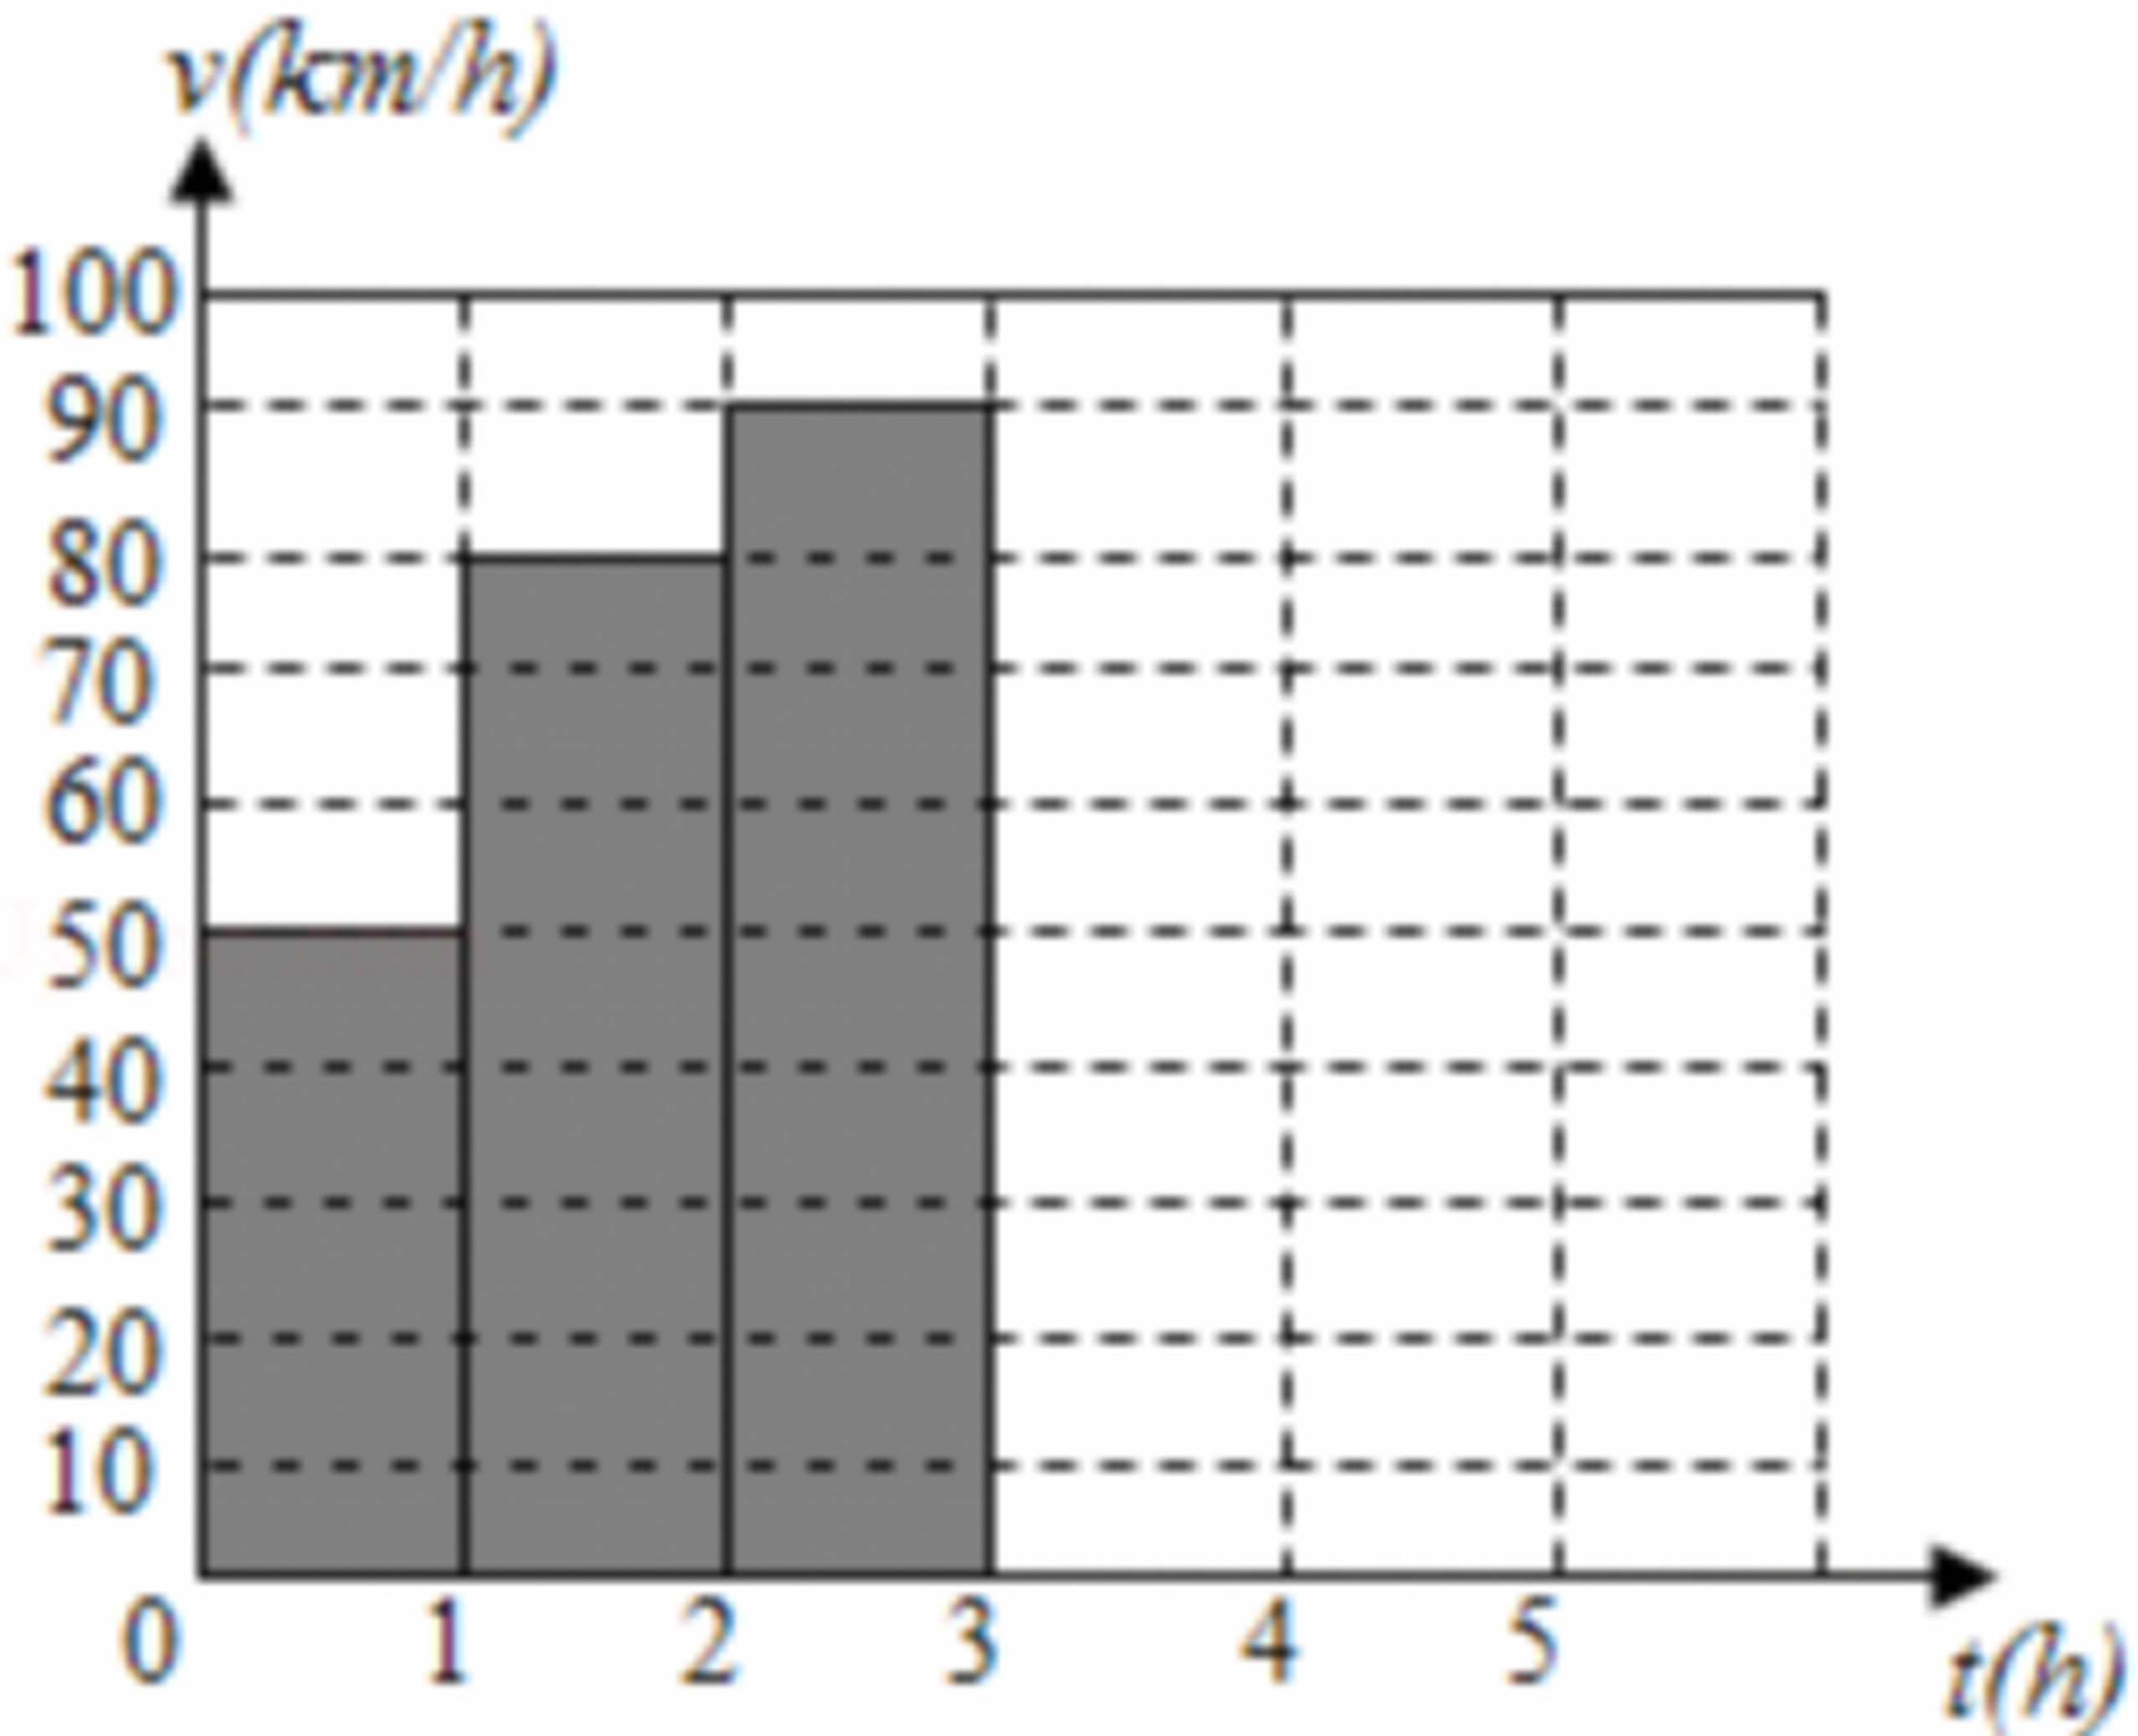
\includegraphics[width=0.52\textwidth]{figures/speed_time_bars.png}
\end{center}

\begin{enumerate}[label=(\arabic*)]
\item 求图中阴影部分的面积，并说明所求面积的实际意义；
\item 假设这辆汽车的里程表在汽车行驶这段路程前的读数为 $2004\,\mathrm{km}$，
试将汽车行驶这段路程时汽车里程表读数 $S$ 表示为时间 $t$ 的函数，
并求出当汽车里程表读数为 $2094\,\mathrm{km}$ 时，汽车行驶了多少时间？
\end{enumerate}

\ifanswer
\solbegin
\stepm{(1)}{由一辆汽车在某段路程中的行驶速度与时间的关系图，}
\step{得阴影部分的面积为 $50\times1+80\times1+90\times1=220$，}
\step{阴影部分的面积表示汽车在 $3$ 小时内行驶的路程为 $220\,\mathrm{km}$.}
\stepm{(2)}{$S=\begin{cases}
50t+2004,&0\leqslant t<1\\
80(t-1)+2054,&1\leqslant t<2\\
90(t-2)+2134,&2\leqslant t\leqslant3
\end{cases}$}
\step{令 $80(t-1)+2054=2094$，解得 $t=1.5$，所以汽车行驶 $1.5$ 小时.}
\solend

\fi

\ansspace[6]

\item 已知集合 $A=\{x\mid x<-2\text{ 或 }x\geqslant3\}$，$U=\R$.

\begin{enumerate}[label=(\arabic*)]
\item 求 $\overline{A}$；
\item 若 $B=\{x\mid mx-1>0\}$，当 $B\sub A$ 时，求实数 $m$ 的取值范围；
\item 若 $B=\{x\mid2m-6\leqslant x\leqslant m+4\}$，当 $B\cap\overline{A}=\varnothing$ 时，
求实数 $m$ 的取值范围.
\end{enumerate}

\ifanswer
\solbegin
\stepm{(1)}{因为集合 $A=\{x\mid x<-2\text{ 或 }x\geqslant3\}$，$U=\R$，
所以 $\overline{A}=\{x\mid-2\leqslant x<3\}$；}
\stepm{(2)}{当 $m=0$ 时，$B=\varnothing$，符合题意，}
\step{当 $m>0$ 时，$B=\left\{x\mid x>\dfrac1m\right\}$，则 $\dfrac1m\geqslant3$，
解得 $0<m\leqslant\dfrac13$，}
\step{当 $m<0$ 时，$B=\left\{x\mid x<\dfrac1m\right\}$，则 $\dfrac1m\leqslant-2$，
解得 $-\dfrac12\leqslant m<0$，}
\step{综上所述，实数 $m$ 的取值范围 $\left[-\dfrac12,\dfrac13\right]$；}
\stepm{(3)}{由题意得 $B=\{x\mid2m-6\leqslant x\leqslant m+4\}$，
$\overline{A}=\{x\mid-2\leqslant x<3\}$，且 $B\cap\overline{A}=\varnothing$，}
\step{当 $B=\varnothing$ 时，$2m-6>m+4$，解得 $m>10$，}
\step{当 $B\neq\varnothing$ 时，则 $\begin{cases}2m-6\leqslant m+4\\ m+4<-2\end{cases}$
或 $\begin{cases}2m-6\leqslant m+4\\ 2m-6\geqslant3\end{cases}$，}
\step{解得 $m<-6$ 或 $\dfrac92\leqslant m\leqslant10$，}
\step{综上所述，实数 $m$ 的取值范围为
$(-\infty,-6)\cup\left[\dfrac92,+\infty\right)$.}
\solend

\fi

\ansspace[8]

\item 在等腰梯形 $ABCD$ 中，$AB=DC=5$，$AD=4$，$BC=10$. 点 $E$ 在下底边 $BC$ 上.
点 $F$ 在腰 $AB$ 上.

\begin{center}
% 图取原卷截图、4× LANCZOS 放大（等腰梯形 $ABCD$ 与线段 $FE$，无辅助线）。
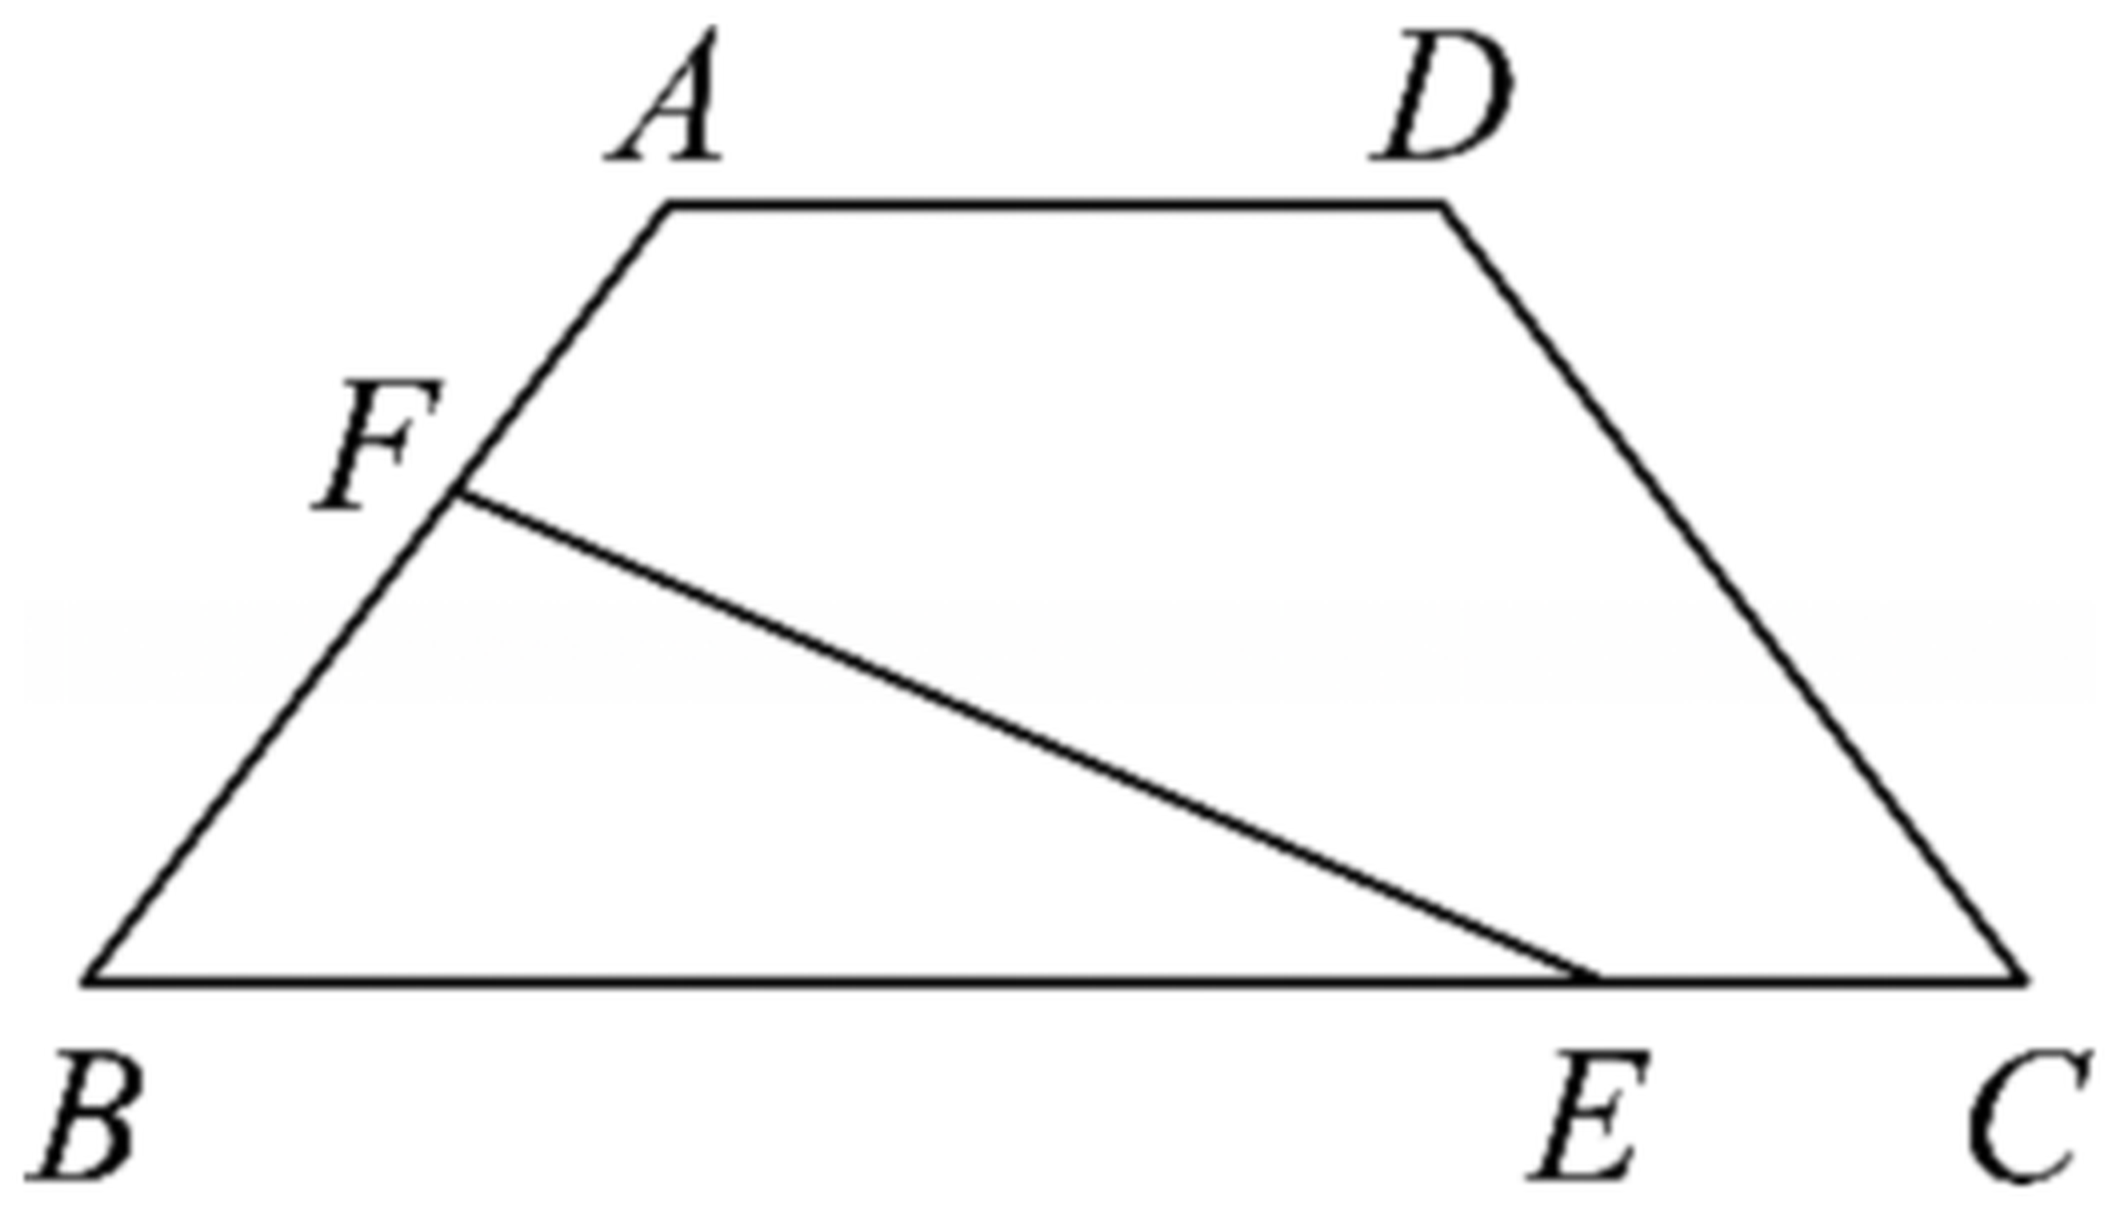
\includegraphics[width=0.46\textwidth]{figures/trapezoid_EF.png}
\end{center}

\begin{enumerate}[label=(\arabic*)]
\item 若 $EF$ 平分等腰梯形 $ABCD$ 的周长，设 $BE$ 长为 $x$，试用含 $x$ 的代数式表示
$\triangle BEF$ 的面积；
\item 是否存在线段 $EF$ 将等腰梯形 $ABCD$ 的周长和面积同时平分？若存在，求出此时 $BE$
的长；若不存在，请说明理由；
\item 是否存在线段 $EF$ 将等腰梯形 $ABCD$ 的周长和面积同时分成 $1:2$ 的两部分？
若存在，求此时 $BE$ 的长；若不存在，请说明理由.
\end{enumerate}

\ifanswer
\solbegin
\stepm{(1)}{过 $A$ 作 $AK\perp BC$ 交 $BC$ 于点 $K$，过 $F$ 作 $FG\perp BC$ 交 $BC$ 于点
$G$，}

\begin{center}
% 图取原卷截图、4× LANCZOS 放大（同梯形，多出虚线 $FG\perp BC$ 与 $AK\perp BC$
% 及两处直角符号；图只在【解析】里出现，故放进 \ifanswer 块）。
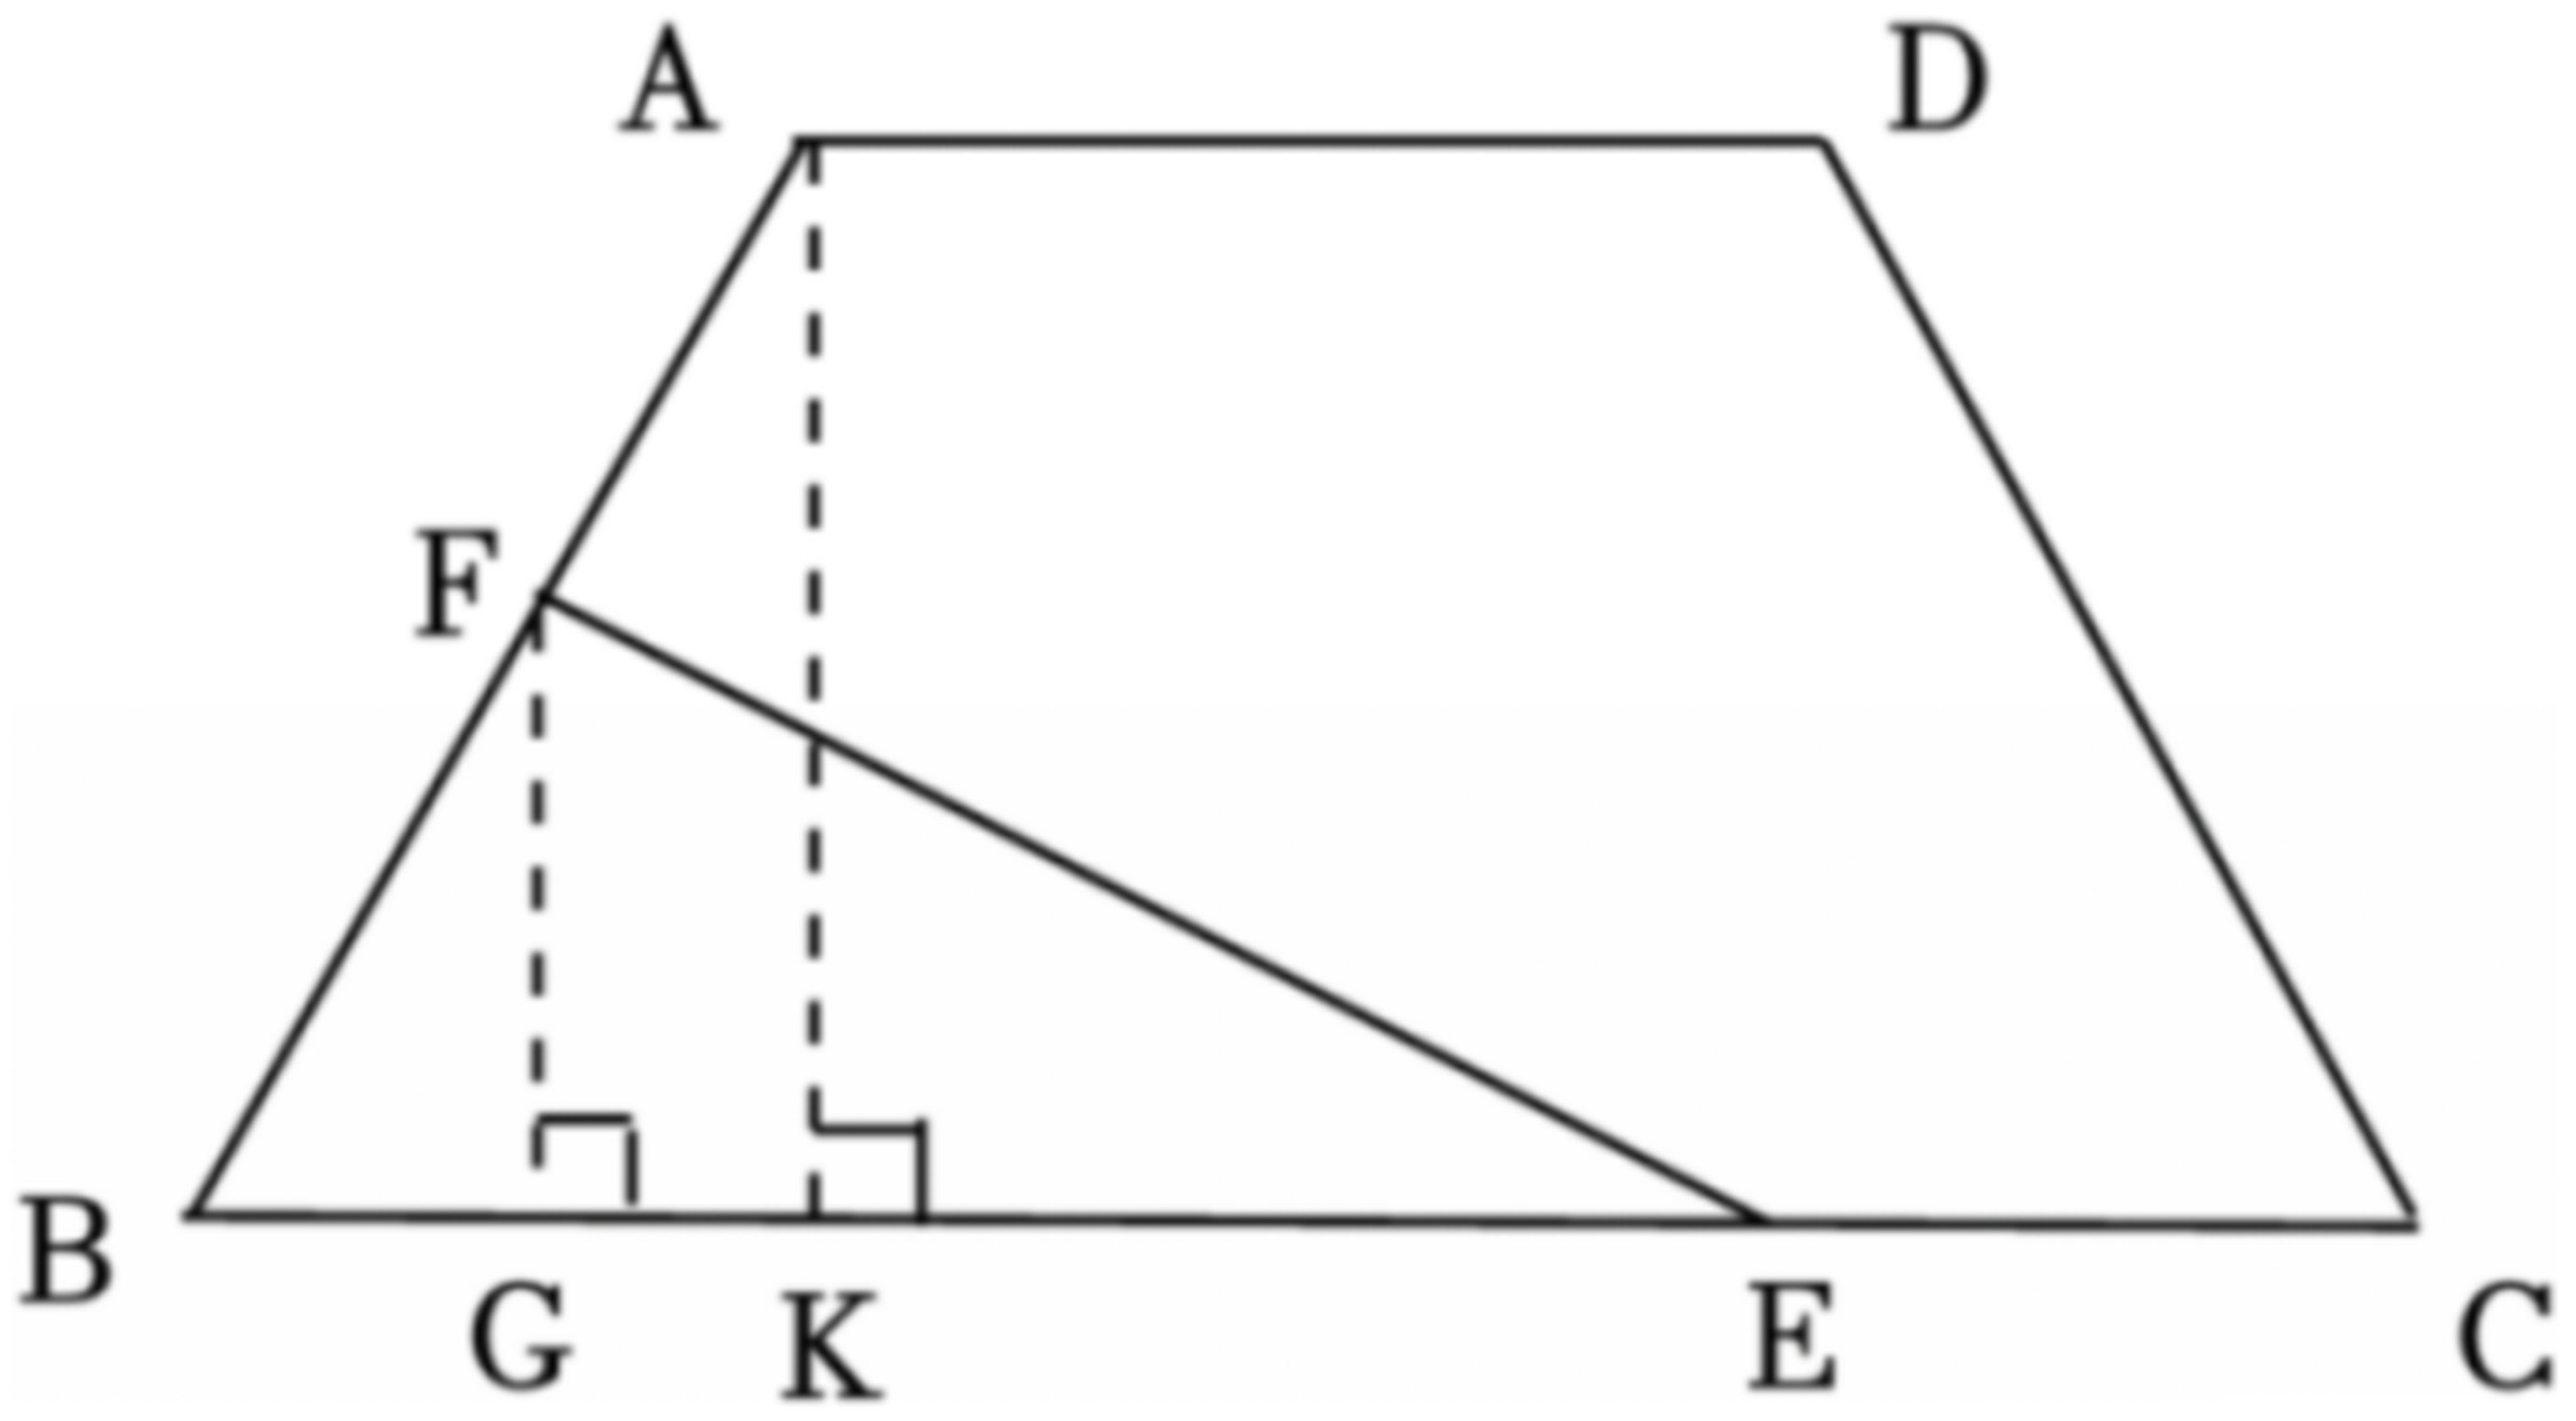
\includegraphics[width=0.62\textwidth]{figures/trapezoid_EF_aux.png}
\end{center}

\step{所以 $BK=\dfrac12\times(BC-AD)=\dfrac12\times(10-4)=3$，}
\step{$AK=\sqrt{AB^2-BK^2}=\sqrt{5^2-3^2}=4$，}
\step{由题意得，梯形 $ABCD$ 周长为 $24$，高为 $4$，面积为 $28$，}
\step{因为 $EF$ 平分等腰梯形 $ABCD$ 的周长，设 $BE$ 长为 $x$，则 $BF=12-x$，}
\step{由 $\begin{cases}0\leqslant12-x\leqslant5\\ 0\leqslant x\leqslant10\end{cases}$，
解得 $7\leqslant x\leqslant10$，}
\step{由题意得 $\triangle BFG\backsim\triangle BAK$，所以 $\dfrac{FG}{AK}=\dfrac{BF}{BA}$，
即 $\dfrac{FG}4=\dfrac{12-x}5$，}
\step{解得 $FG=\dfrac45(12-x)$，}
\step{所以 $S_{\triangle BEF}=\dfrac12BE\cdot FG
=-\dfrac25x^2+\dfrac{24}5x$（$7\leqslant x\leqslant10$）；}
\stepm{(2)}{存在，由 (1) 得 $-\dfrac25x^2+\dfrac{24}5x=\dfrac{28}2$，$x\in[7,10]$，}
\step{即 $x^2-12x+35=0$，解得 $x=7$ 或 $x=5$（舍去），}
\step{所以存在线段 $EF$ 将等腰梯形 $ABCD$ 的周长和面积同时平分，此时 $BE=7$；}
\stepm{(3)}{不存在，}
\step{情况一：$\triangle BEF$ 的面积$:$多边形 $AFECD$ 的面积 $=1:2$，
$(BE+BF):(AF+AD+DC+CE)=1:2$，}
\step{梯形周长的 $\dfrac13$ 是 $\dfrac{24}3=8$，面积的 $\dfrac13$ 是 $\dfrac{28}3$，}
\step{又因为 $BE=x$，所以 $BF=8-x$，}
\step{又因为 $\dfrac{FG}{AK}=\dfrac{BF}{BA}$，即 $\dfrac{FG}4=\dfrac{8-x}5$，
所以 $FG=\dfrac{32-4x}5$，}
\step{所以 $S_{\triangle BEF}=\dfrac12BE\times FG=-\dfrac25x^2+\dfrac{16}5x$，
所以 $\dfrac{28}3=-\dfrac25x^2+\dfrac{16}5x$，}
\step{整理得 $-3x^2+24x-70=0$，此时 $\Delta<0$，无解，故不存在；}
\step{情况二：$\triangle BEF$ 的面积$:$多边形 $AFECD$ 的面积 $=2:1$，
$(BE+BF):(AF+AD+DC+CE)=2:1$，}
\step{梯形周长的 $\dfrac13$ 为 $\dfrac{24}3=8$，面积的 $\dfrac13$ 为 $\dfrac{28}3$，
又 $BE=x$，所以 $BF=16-x$，}
\step{又 $\dfrac{FG}{AK}=\dfrac{BF}{BA}$，即 $\dfrac{FG}4=\dfrac{16-x}5$，
所以 $FG=\dfrac{64-4x}5$，}
\step{所以 $S_{\triangle BEF}=\dfrac12BE\times FG=-\dfrac25x^2+\dfrac{32}5x$，}
\step{所以 $\dfrac{28}3\times2=-\dfrac25x^2+\dfrac{32}5x$，
整理得 $-3x^2+48x-140=0$，}
\step{解得 $x=\dfrac{48+\sqrt{624}}6>10$，$x=\dfrac{48-\sqrt{624}}6<7$，
不符合题意，舍去，故不存在；}
\step{综上所述，不存在线段 $EF$ 将等腰梯形 $ABCD$ 的周长和面积同时分成 $1:2$ 的两部分.}
\solend

\fi

\ansspace[8]

\item 对集合 $\{1,2,\cdots,n\}$ 及其每一个非空子集 $A$，定义一个唯一确定的“交替和”
如下：将 $A$ 中的元素按照递减的次序排列，然后将第一个元素交替地减或加后继的元素所得的
结果，例如，子集 $\{1,2,4,6,9\}$ 的“交替和”是 $9-6+4-2+1=6$，子集 $\{5,6\}$ 的
“交替和”是 $6-5=1$，子集 $\{2\}$ 的交替和是 $2$；定义一个唯一确定的“交替积”如下：
将 $A$ 中的元素按照递减的次序排列，然后将第一个元素交替地除以或乘以后继的数所得的结果，
例如，集合 $\{1,2,4,6,9\}$ 的“交替积”是 $9\div6\times4\div2\times1=3$，
$\{5,6\}$ 的“交替积”是 $6\div5=1.2$，$\{2\}$ 的“交替积”是 $2$.

\begin{enumerate}[label=(\arabic*)]
\item 对于 $\{1,2,3,4,5,6,7,8,9\}$，求其所有子集的“交替和”的总和；
\item 对于 $\{1,2,\cdots,n\}$，求其所有子集的“交替和”的总和；
\item 对于 $\left\{n\mid\dfrac{495}{n+2}\in\N,n\in\Z\right\}$ 求其所有子集的
“交替积”的总和.
\end{enumerate}

\ifanswer
\solbegin
\stepm{(1)}{集合 $\{1,2,3,4,5,6,7,8,9\}$ 的子集中，除去 $\{9\}$ 外还有 $2^9-2$ 个
非空子集，}
\step{把这 $2^9-2$ 个非空子集两两组合后分别计算每一组中“交替和”之和，}
\step{组合原则是设 $A_i=\{9,a_1,a_2,\cdots\}$，$A_i^1=\{a_1,a_2,\cdots\}$，}
\step{集合 $A_i^1$ 的元素为集合 $A_i$ 中去掉 $9$ 的所有元素，把 $A_i$ 和 $A_i^1$
结合为一组，}
\step{显然，每组的“交替和”的和为 $9$，共有 $\dfrac{2^9-2}2$ 组，}
\step{所以，所有“交替和”之和应该为 $\dfrac{9(2^9-2)}2+9=2304$；}
\stepm{(2)}{集合 $\{1,2,\cdots,n\}$ 的子集中，除去 $\{n\}$ 外还有 $2^n-2$ 个非空子集，}
\step{把这 $2^n-2$ 个非空子集两两组合后分别计算每一组中“交替和”之和，}
\step{组合原则是设 $A_i=\{n,a_1,a_2,\cdots\}$，$A_i^1=\{a_1,a_2,\cdots\}$，}
\step{集合 $A_i^1$ 的元素为集合 $A_i$ 中去掉 $n$ 的所有元素，把 $A_i$ 和 $A_i^1$
结合为一组，}
\step{显然，每组的“交替和”的和为 $n$，共有 $\dfrac{2^n-2}2$ 组，}
% 注：下一行分子原卷印作花括号（其余同类处皆用圆括号），照抄未改，见文件头“原卷存疑”③。
\step{所以，所有“交替和”之和应该为 $\dfrac{n\{2^n-2\}}2+n=n\cdot2^{n-1}$；}
\stepm{(3)}{集合 $\left\{n\mid\dfrac{495}{n+2}\in\N,n\in\Z\right\}
=\{493,163,97,53,43,31,13,9,7,3,1,-1\}$，}
\step{其中除去 $\{-1\}$ 外还有 $2^{12}-2$ 个非空子集，}
% 注：下一行原卷把“把这”重复印了一次（“把这把这”），照抄未改，见文件头“原卷存疑”②。
\step{把这把这 $2^{12}-2$ 个非空子集两两组合后分别计算每一组中“交替积”之和，}
\step{组合原则是设 $A_j=\{-1,a_1,a_2,\cdots\}$，$A_j^1=\{a_1,a_2,\cdots\}$，}
\step{集合 $A_j^1$ 的元素为集合 $A_j$ 中去掉 $-1$ 的所有元素，把 $A_j$ 和 $A_j^1$
结合为一组，}
\step{显然，每组的“交替积”的和为 $0$，共有 $\dfrac{2^{12}-2}2$ 组，}
\step{所以，所有“交替积”之和应该为 $\dfrac{2^{12}-2}2\times0-1=-1$.}
\solend

\fi

\ansspace*[10]

\end{enumerate}

\end{document}
"
%
% 原始材料是微信公众号图文（公众号“魔都数学加油站”连载“27学年高一 30”，2026-09-23 发布，
% 原文标题“27学年高一30——2026-2027年上海市南洋模范中学高一上开学考”），
% 正文为 11 张 PNG 页。**同一篇里各页分辨率不一致**——第 2、3、9、10 页 4762×6735，
% 其余七页 2560×3620（已逐页打开确认，非下载缺档），取的是 mmbiz.qpic.cn/<hash>/0 的原图档。
% 原文本身就是一份**讲评版**：填空第 3—7 题下方印【答案】，第 8—12 题与其后各题印【解析】。
% 试题文字、答案与解析均照原卷录入，未改内容。卷面的粉色斜水印属水印，未录入。
%
% 卷首标题：原卷印作“2026-2027 年南洋模范中学高一上开学考”（公众号标题里的“上海市”
% 三字卷面标题行没有，本稿照卷面），年份区间按全稿惯例排 en dash，前缀照原卷保留“年”。
%
% 与原卷的排版差异（均已在 README“说明”中交代）：
%   ① 原文自**第 3 题**起（第 1、2 题未在该文中发布），故本稿题号亦自 3 起；
%   ② 原卷本就印有“一、填空题”“二、选择题”“三、解答题”三节标题，本稿照原卷分节，
%      只把标题改排成全稿统一的“大节标题”样式；
%   ③ 原卷填空第 3—7 题只印【答案】行、第 8 题起印【解析】（选择题答案写在解析末句
%      “故选 D／B”里），本稿统一改为试卷版隐去、答案版以 \ans{}／\ifanswer 块给出，
%      两版彻底分离；
%   ④ 子集符号原卷两种并用：第 7 题题干两处、第 19(2) 题作带下划线的 $\subseteq$，
%      第 17(2) 题解析作真包含的 $\subset$，本稿分别照录为 $\sub$ 与 $\subset$；
%   ⑤ 补集符号原卷一律作**上横线**（$\overline{A}$、$\overline{B}$），本稿照录；
%   ⑥ 原卷的实数集 R 一律作斜体（第 4 题、第 17 题与第 19 题题干的 $U=R$），
%      第 21(3) 题的自然数集与整数集作**粗体** $\mathbf{N}$、$\mathbf{Z}$，
%      本稿按全稿惯例统一写作 $\R$、$\N$、$\Z$；
%   ⑦ 原卷填空的横线约两个字宽，本稿按全稿惯例统一排 \blankline[4.4em]；
%   ⑧ 原卷未印副标题，本稿按全稿惯例补出副标题“集合与常用逻辑用语”——但本卷是开学考，
%      范围不止这一章：第 18 题是速度—时间图象题、第 20 题是等腰梯形的周长/面积平分问题，
%      副标题只标了主章节（见文末“高一30 专记”）；
%   ⑨ 第 13、14、18、20 题的图印在题干右侧、第 16 题的三幅图印在【解析】里的下一页顶部、
%      第 20 题【解析】另有一张带辅助线的图，本稿一律移至题干或解析之后；
%      图取原卷截图、4× LANCZOS 放大（见各 \includegraphics 前的注释）。
%
% 原卷存疑三处（均照抄原卷、未改，见源码中该处上方注释）：
%   ① 第 10 题【解析】验证“破晓集”时写的是 $\notin A$、$\in A$（如“$-2-2=-4\notin A$”），
%      但该处讨论的集合原题设里叫 $P$，同题②的“$x+y=2(k_1+k_2)\in A$”亦然——
%      本稿照抄未改（按文意应为 $P$）；
%   ② 第 21 题【解析】(3) 有“把这把这 $2^{12}-2$ 个非空子集”（“把这”重复印了一次）；
%   ③ 同题 (2) 的结论式分子原卷印作花括号 $\dfrac{n\{2^n-2\}}{2}$（其余同类处皆用圆括号）。

\documentclass[a4paper,11pt]{article}
\usepackage{common}

\begin{document}

\examtitlest[3]{2026--2027 年南洋模范中学高一上开学考}{集合与常用逻辑用语}

\bigsec{一、填空题}

\begin{enumerate}
\setcounter{enumi}{2}

\item 若集合 $A=\{x\mid x^2-2kx+7k=0\}$ 有且仅有三个真子集，则 $k$ 的取值范围是
\blankline[4.4em].

\ans{$(-\infty,0)\cup(7,+\infty)$}

\item “存在 $x\in\R$，使得 $x^2+2x+5=0$”的否定形式是 \blankline[4.4em].

\ans{对任何 $x\in\R$，都有 $x^2+2x+5\neq0$}

\item 下列命题中，$p$ 是 $q$ 的必要非充分条件的是 \blankline[4.4em].

① $p:x>2$ 且 $y>3$，$q:x+y>5$；

② $p$：四边形的四个角都相等，$q$：四边形是正方形.

\ans{②}

\item 若“条件 $\alpha:2\leqslant x\leqslant4$”是“条件 $\beta:3m-1\leqslant x\leqslant-m$”的
充分非必要条件，则 $m$ 的取值范围是 \blankline[4.4em].

\ans{$(-\infty,-4]$}

\item 满足 $\{1\}\sub M\sub\{1,2,4,5\}$ 的集合 $M$ 的个数为 \blankline[4.4em] 个.

\ans{$8$}

\item 已知集合 $A=\{1,2\}$，集合 $B=\{x\mid ax=6\}$，若 $A\cup B=A$，则 $a$ 的所有取值
构成的集合为 \blankline[4.4em].

\ifanswer
\solbegin
\step{因为 $A\cup B=A$，所以 $B\sub A$，}
\step{当 $a=0$ 时，$B=\varnothing$，满足 $B\sub A$；}
\step{当 $a\neq0$ 时，$B=\left\{\dfrac6a\right\}$，则 $\dfrac6a=1$ 或 $\dfrac6a=2$，
解得 $a=6$ 或 $a=3$，}
\step{综上所述，$a$ 的所有取值构成的集合为 $\{0,3,6\}$.}
\solend

\fi

\item 对于集合 $M$、$N$，定义 $M-N=\{x\mid x\in M\text{ 且 }x\notin N\}$，
$M\oplus N=(M-N)\cup(N-M)$，设 $A=\{y\mid y=|x|,x\in\R\}$，
$B=\{y\mid y=-(x-1)^2+2,x\in\R\}$，则 $A\oplus B=$ \blankline[4.4em].

\ifanswer
\solbegin
\step{由已知 $A=[0,+\infty)$，$B=(-\infty,2]$，}
\step{由于 $A-B=(2,+\infty)$，$B-A=(-\infty,0)$，}
\step{故 $A\oplus B=(A-B)\cup(B-A)=(-\infty,0)\cup(2,+\infty)$.}
\solend

\fi

\item 设 $P$ 为非空实数集满足：对任意给定的 $x$、$y\in P$（$x$、$y$ 可以相同），都有
$x+y\in P$，$x-y\in P$，$xy\in P$，则称 $P$ 为破晓集. 关于破晓集有下列结论：
①集合 $P=\{-2,-1,0,1,2\}$ 为破晓集；②集合 $P=\{x\mid x=2n,n\in\Z\}$ 为破晓集；
③若集合 $P_1$、$P_2$ 为破晓集，则 $P_1\cup P_2$ 为破晓集；④若集合 $P$ 为破晓集，
则一定有 $0\in P$；⑤若集合 $P_1$、$P_2$ 为破晓集，则 $P_1\cap P_2$ 为破晓集；
其中正确结论的序号是 \blankline[4.4em].

\ifanswer
\solbegin
% 注：以下几步原卷把该集合记作 $A$（题设里叫 $P$），照抄未改，见文件头“原卷存疑”①。
\step{对于①：$-2-2=-4\notin A$，故集合 $P=\{-2,-1,0,1,2\}$ 不为破晓集，故①错误；}
\step{②设 $x$、$y\in A$，则 $x=2k_1$，$y=2k_2$，且 $k_1$、$k_2\in\Z$，}
\step{故 $x+y=2(k_1+k_2)\in A$，$x-y=2(k_1-k_2)\in A$，$xy=4k_1k_2\in A$，}
\step{故集合 $P=\{x\mid x=2n,n\in\Z\}$ 为破晓集，故②正确；}
\step{③若集合 $P_1$、$P_2$ 为破晓集，设 $P_1=\{x\mid x=2k,k\in\Z\}$，
$P_2=\{x\mid x=3k,k\in\Z\}$，}
\step{但是 $P_1\cup P_2$ 不为破晓集，如 $x=2$，$y=3$ 时，$x+y=5$，
故 $5\notin(P_1\cup P_2)$，故③错误；}
\step{④若集合 $P$ 为破晓集，则取 $x=y$，$x-y=0\in A$，则一定有 $0\in P$，故④正确.}
\step{⑤正确；}
\step{故正确的是②④⑤.}
\solend

\fi

\item 已知集合 $M$ 的元素均为正整数，定义集合 $M$ 的“变项和”为：将 $M$ 中每个元素 $m$
都乘以 $(-1)^m$ 后再求和. 若集合 $A=\{n\mid1\leqslant n\leqslant10,n\in\N\}$，则集合 $A$
的所有非空子集的“变项和”的总和为 \blankline[4.4em].

\ifanswer
\solbegin
\step{$A$ 集合的所有非空子集中，每个元素出现的次数都是
$(2^{10}-1)-(2^9-1)=2^9$，}
\step{则集合 $A$ 的所有非空子集的“变项和”的总和为
$1\times(-1)^1\times2^9+2\times(-1)^2\times2^9+\cdots+10\times(-1)^{10}\times2^9$}
\step{$=(-1+2-3+4-\cdots-9+10)\times2^9=5\times2^9=2560$.}
\solend

\fi

\item 已知集合 $A=[t,t+1]\cup[t+4,t+9]$，$0\notin A$，存在正数 $\lambda$，使得对任意
$a\in A$，都有 $\dfrac\lambda a\in A$，则 $t$ 的值是 \blankline[4.4em].

\ifanswer
\solbegin
\step{当 $t>0$ 时，当 $a\in[t,t+1]$ 时，$\dfrac\lambda a\in[t+4,t+9]$，}
\step{当 $a\in[t+4,t+9]$ 时，$\dfrac\lambda a\in[t,t+1]$，}
\step{即当 $a=t$ 时，$\dfrac\lambda a\leqslant t+9$；当 $a=t+9$ 时，
$\dfrac\lambda a\geqslant t$，即 $\lambda=t(t+9)$；}
\step{当 $a=t+1$ 时，$\dfrac\lambda a\geqslant t+4$，当 $a=t+4$ 时，
$\dfrac\lambda a\leqslant t+1$，即 $\lambda=(t+1)(t+4)$，}
\step{所以 $t(t+9)=(t+1)(t+4)$，解得 $t=1$.}
\step{当 $t+1<0<t+4$ 时，当 $a\in[t,t+1]$ 时，$\dfrac\lambda a\in[t,t+1]$.}
\step{当 $a\in[t+4,t+9]$ 时，则 $\dfrac\lambda a\in[t+4,t+9]$，}
\step{即当 $a=t$ 时，$\dfrac\lambda a\leqslant t+1$，当 $a=t+1$ 时，
$\dfrac\lambda a\geqslant t$，即 $\lambda=t(t+1)$，}
\step{即当 $a=t+4$ 时，$\dfrac\lambda a\leqslant t+9$，当 $a=t+9$ 时，
$\dfrac\lambda a\geqslant t+4$，即 $\lambda=(t+4)(t+9)$，}
\step{所以 $t(t+1)=(t+4)(t+9)$，解得 $t=-3$.}
\step{当 $t+9<0$ 时，同理可得无解.}
\step{综上，$t$ 的值为 $1$ 或 $-3$.}
\solend

\fi

\end{enumerate}

\bigsec{二、选择题}

\begin{enumerate}
\setcounter{enumi}{12}

% 这道题是“题干 + 图 + 选项”约 6cm 的一整块，页末放不下就会被拆开（切页审计的 A 类），
% 故在题前先量一次页高：不够就把整道题干连图带选项一起挪到次页。
\needvspace{6.5cm}
\item 设 $U=\{1,2,3,4,5\}$，$A$、$B$ 都是 $U$ 的子集，且 $A\cap B=\{5\}$，
$\overline{A}\cap B=\{4\}$，$\overline{A}\cap\overline{B}=\{1,2\}$，
则以下四个判断中正确的是\mbox{（\quad）}

\begin{center}
% 图取原卷截图、4× LANCZOS 放大（原卷把图印在题干右侧，本稿移至此处，见文件头⑨）。
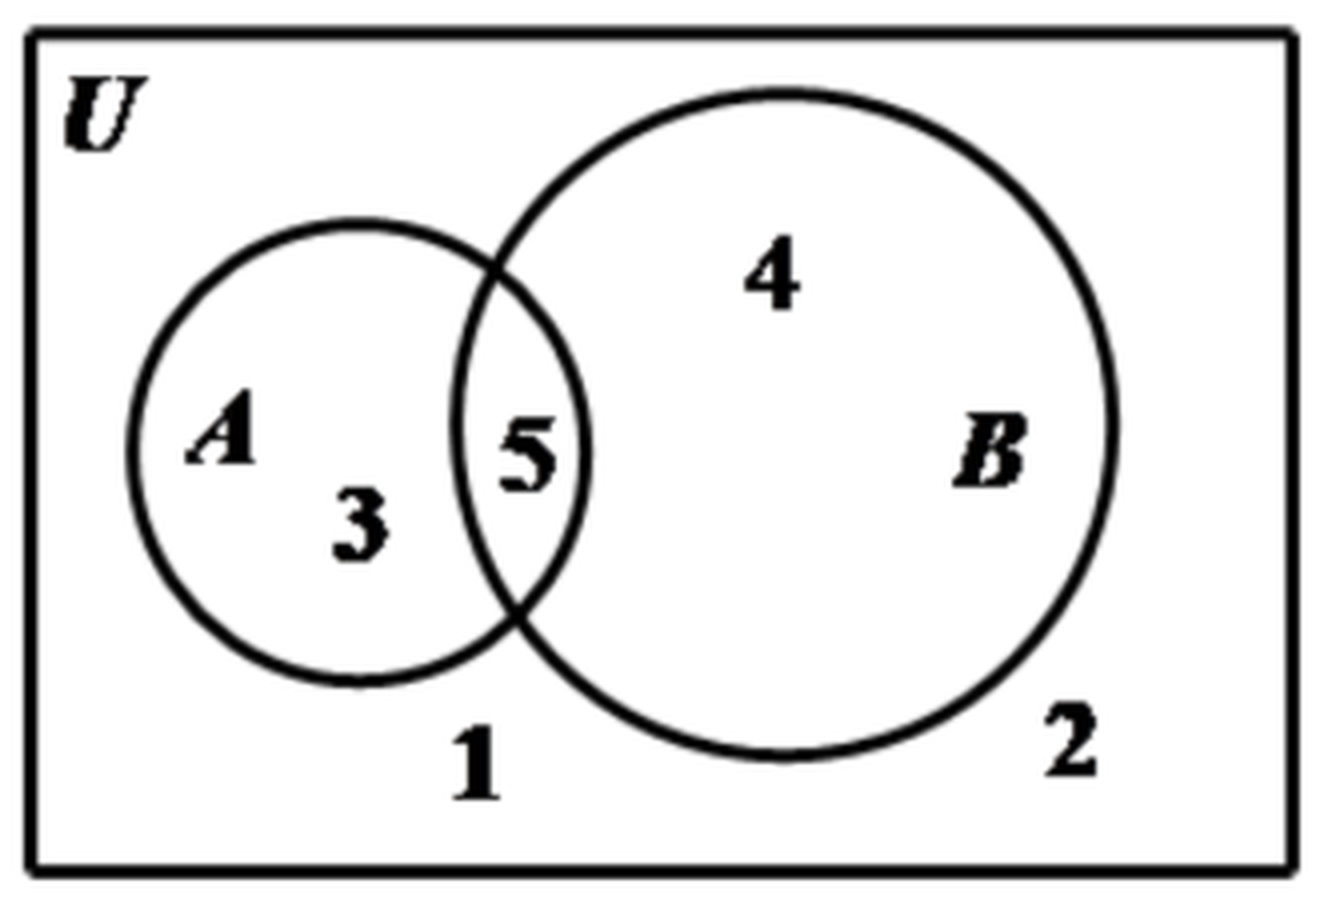
\includegraphics[width=0.28\textwidth]{figures/venn_U5_AB.png}
\end{center}

\keepwithprev
A. $3\notin A$ 且 $3\notin B$\qquad\qquad B. $3\in A$ 且 $3\in B$

C. $3\notin A$ 且 $3\in B$\qquad\qquad D. $3\in A$ 且 $3\notin B$

\ans{$D$}

\ifanswer
\solbegin
\step{画出韦恩图，得 $A=\{5,3\}$，$B=\{5,4\}$，}
\step{则 $3\in A$ 且 $3\notin B$. 故选 $D$.}
\solend

\fi

% 同第 13 题：整块（题干 + 图 + 选项）在答案版还要再挂【答案】【解析】，页末更易被拆开。
\needvspace{7.5cm}
\item 如图表示图形阴影部分的是\mbox{（\quad）}

\begin{center}
% 图取原卷截图、4× LANCZOS 放大（三圆 $A$、$B$、$C$，阴影为整个 $A$ 圆加 $B\cap C$）。
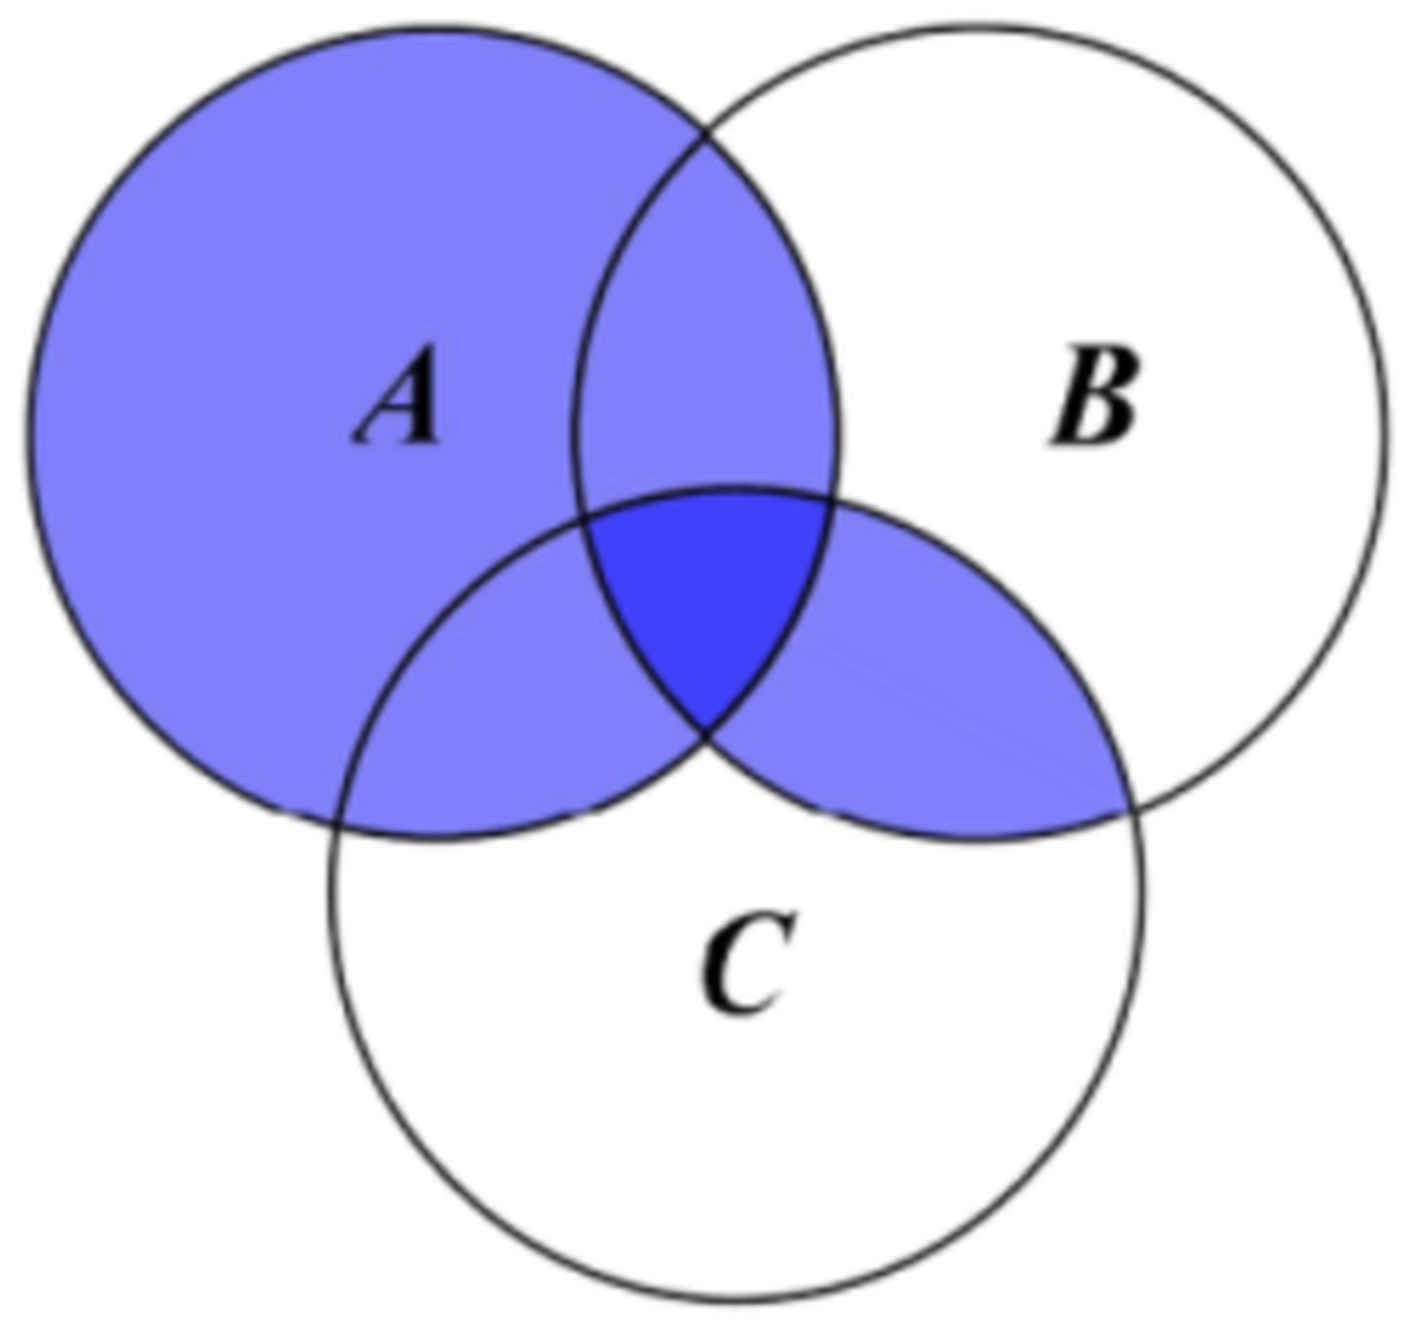
\includegraphics[width=0.30\textwidth]{figures/venn_A_union_BC.png}
\end{center}

\keepwithprev
A. $(A\cup C)\cap(B\cup C)$\qquad\qquad B. $(A\cup B)\cap(A\cup C)$

C. $(A\cup B)\cap(B\cup C)$\qquad\qquad D. $(A\cup B)\cap C$

\ans{$B$}

\ifanswer
\solbegin
\step{图中阴影部分表示元素满足是 $A$ 中的元素，或者是 $B$ 与 $C$ 的公共元素，}
\step{故可以表示为 $A\cup(B\cap C)$，也可以表示为 $(A\cup B)\cap(A\cup C)$.
故选 $B$.}
\solend

\fi

\item 设集合 $M=\left\{x\mid m\leqslant x\leqslant m+\dfrac34\right\}$，
$N=\left\{x\mid n-\dfrac13\leqslant x\leqslant n\right\}$，且 $M$、$N$ 都是集合
$\{x\mid0\leqslant x\leqslant1\}$ 的子集，如果把 $b-a$ 叫做集合
$\{x\mid a\leqslant x\leqslant b\}$ 的“长度”，那么集合 $M\cap N$ 的“长度”的
最小值是\mbox{（\quad）}

\keepwithprev
A. $\dfrac23$\qquad B. $\dfrac1{12}$\qquad C. $\dfrac13$\qquad D. $\dfrac5{12}$

\ans{$B$}

\ifanswer
\solbegin
\step{$M$ 的长度为 $\dfrac34$，$N$ 的长度为 $\dfrac13$，}
\step{当集合 $M\cap N$ 的长度的最小值时，$M$ 与 $N$ 应分别在区间 $[0,1]$ 的左右两端，}
\step{故 $M\cap N$ 的长度的最小值是 $\dfrac34+\dfrac13-1=\dfrac1{12}$，故选 $B$.}
\solend

\fi

\item 定义集合运算 $A-B=\{x\mid x\in A\text{ 且 }x\notin B\}$ 称为集合 $A$ 与集合 $B$ 的
差集；定义集合运算 $A\Delta B=(A-B)\cup(B-A)$ 称为集合 $A$ 与集合 $B$ 的对称差，
有以下 $4$ 个等式：① $A\Delta B=B\Delta A$；② $(A\Delta B)\Delta C=A\Delta(B\Delta C)$；
③ $A\cap(B\Delta C)=(A\cap B)\Delta(A\cap C)$；
④ $A\cup(B\Delta C)=(A\cup B)\Delta(A\cup C)$，
则 $4$ 个等式中恒成立的是\mbox{（\quad）}

\keepwithprev
A. ①②\qquad B. ①②③\qquad C. ①②④\qquad D. ①②③④

\ans{$B$}

\ifanswer
\solbegin
\step{对于①，由 $B\Delta A=(B-A)\cup(A-B)=(A-B)\cup(B-A)=A\Delta B$，
所以①正确；}
\step{对于②，由 $A-B=\{x\mid x\in A\text{ 且 }x\notin B\}
=\{x\mid x\in A,x\notin(A\cap B)\}=A-(A\cap B)$，}
\step{同理可得 $B-A=B-(A\cap B)$，}
\step{则 $A\Delta B=(A-B)\cup(B-A)=(A\cup B)-(A\cap B)$，}
\step{所以 $(A\Delta B)\Delta C=(A\Delta B)\cup C-(A\Delta B)\cap C$，}
\step{所以表示的集合为图（1）中阴影部分所表示的集合，如图所示，}
\step{同理 $A\Delta(B\Delta C)=A\cup(B\Delta C)-A\cap(B\Delta C)$，
也表示图（1）中阴影部分所表示的集合，}
\step{所以 $(A\Delta B)\Delta C=A\Delta(B\Delta C)$，所以②正确；}

\begin{center}
% 图取原卷截图、4× LANCZOS 放大（原卷印在下一页顶部，共三幅三圆韦恩图：
% 图（1）一幅、图（2）左右两幅，图（2）两幅下方各有一行式子标注）。
% 图只在【解析】里出现，故放进 \ifanswer 块，试卷版不排。
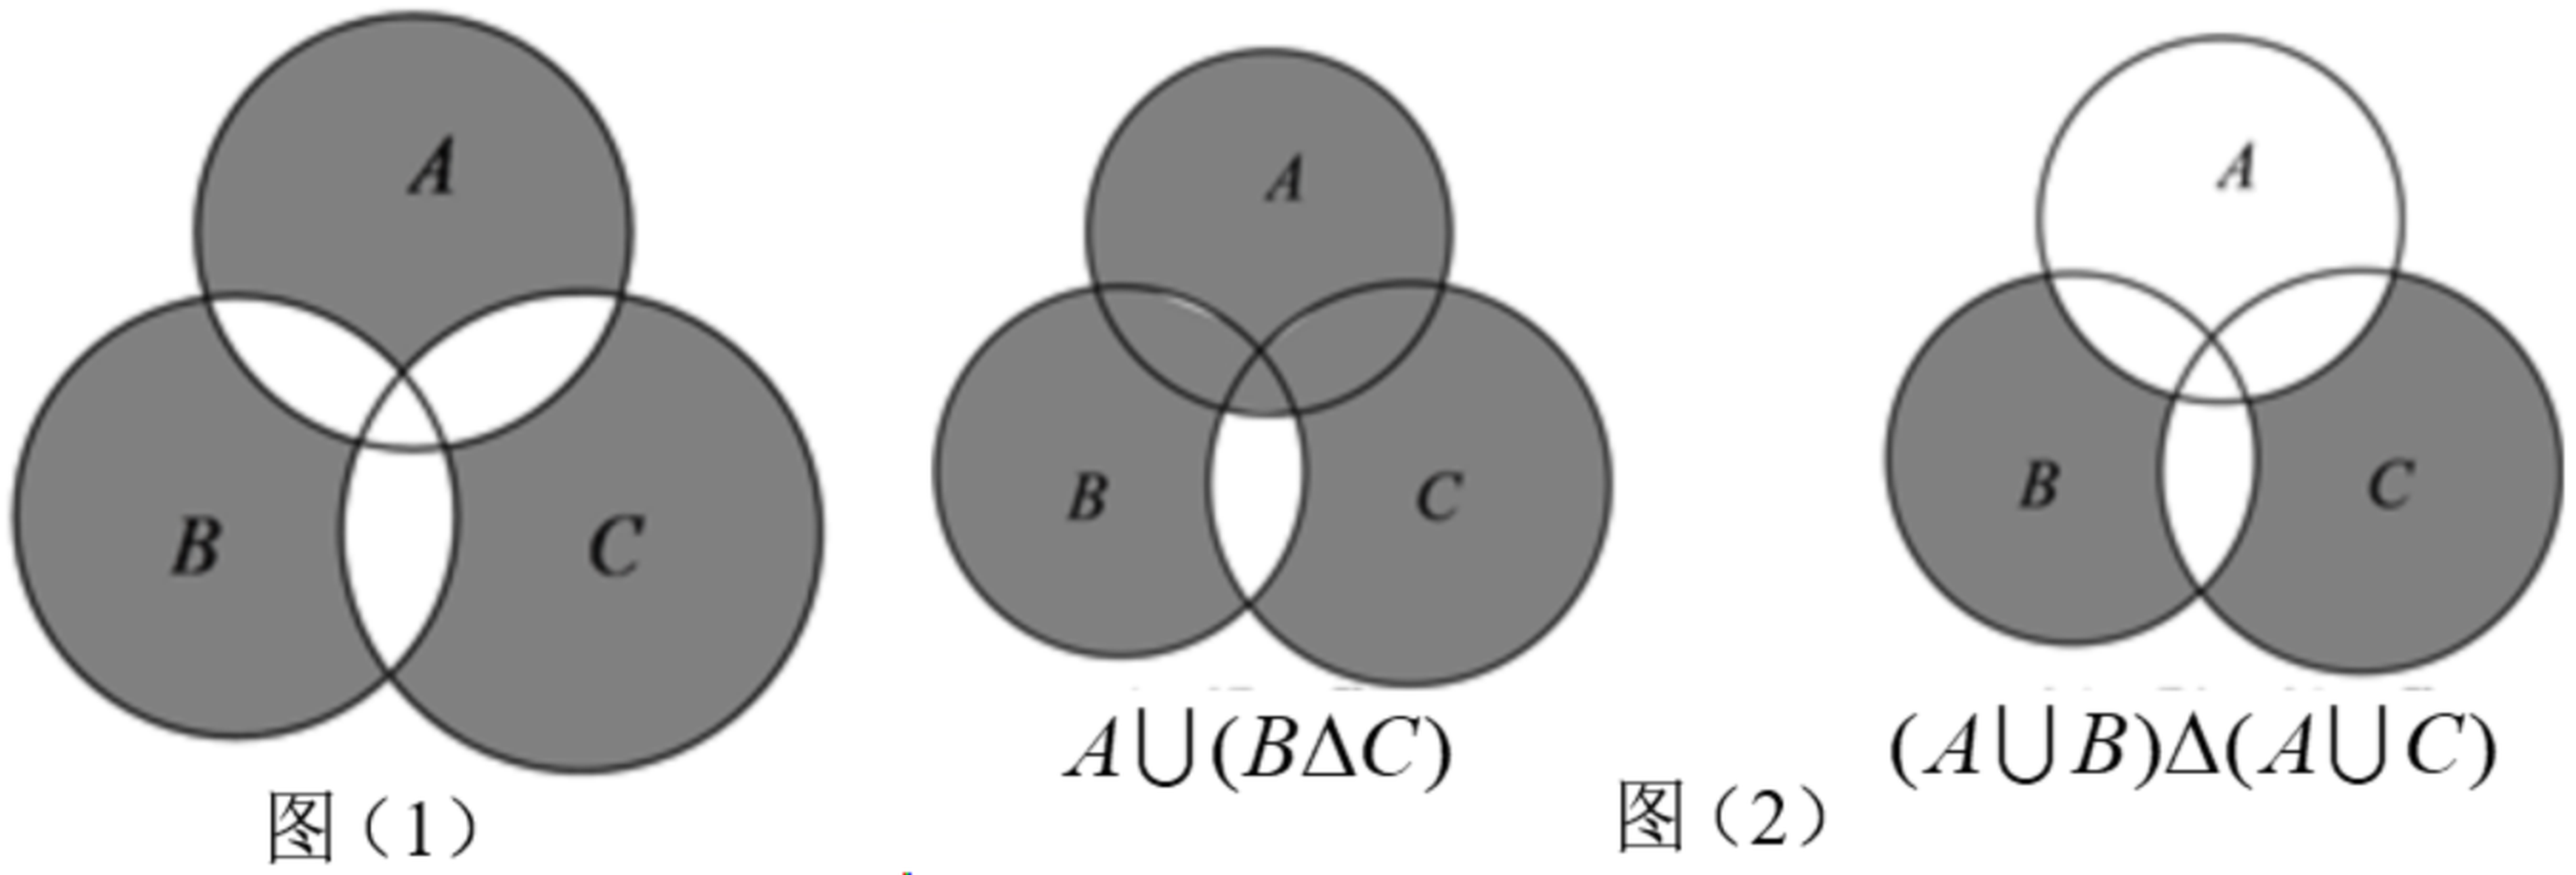
\includegraphics[width=0.86\textwidth]{figures/venn_symdiff3.png}
\end{center}

\step{对于③，由 $A\cap(B\Delta C)=A\cap(B\cup C-B\cap C)
=A\cap(B\cup C)-A\cap(B\cap C)$}
\step{$=(A\cap B)\cup(A\cap C)-(A\cap B)\cap(A\cap C)=(A\cap B)\Delta(A\cap C)$，
所以③正确；}
\step{对于④，如图（2）所示，$A\cup(B\Delta C)\neq(A\cup B)\Delta(A\cup C)$，
所以④错误.}
\step{故选 $B$.}
\solend

\fi

\end{enumerate}

\bigsec{三、解答题}

\begin{enumerate}
\setcounter{enumi}{16}

\item 已知集合 $M=\{x\mid a-1\leqslant x\leqslant2a+3\}$，$P=\{x\mid-2<x\leqslant4\}$，
全集 $U=\R$.

\begin{enumerate}[label=(\arabic*)]
\item 当 $a=2$ 时，求 $M\cap P$；
\item 若 $x\in P$ 是 $x\in M$ 的必要不充分条件，求实数 $a$ 的取值范围.
\end{enumerate}

\ifanswer
\solbegin
\stepm{(1)}{当 $a=2$ 时，集合 $M=\{x\mid1\leqslant x\leqslant7\}$，}
\step{所以 $M\cap P=\{x\mid1\leqslant x\leqslant4\}$；}
\stepm{(2)}{因为 $x\in P$ 是 $x\in M$ 的必要不充分条件，所以 $M\subset P$，}
\step{当 $M=\varnothing$ 时，$a-1>2a+3$，解得 $a<-4$，}
\step{当 $M\neq\varnothing$ 时，则
$\begin{cases}a-1\leqslant2a+3\\ a-1>-2\\ 2a+3\leqslant4\end{cases}$，
解得 $-1<a\leqslant\dfrac12$，}
\step{综上所述，实数 $a$ 的取值范围为
$(-\infty,-4)\cup\left(-1,\dfrac12\right]$.}
\solend

\fi

\ansspace[6]

\item 一辆汽车在某段路程中的行驶速度与时间的关系如图：

\begin{center}
% 图取原卷截图、4× LANCZOS 放大（速度—时间图：纵轴 $v/(\mathrm{km/h})$、
% 横轴 $t(\mathrm{h})$，$t\in[0,1]$、$[1,2]$、$[2,3]$ 三段矩形条高 50、80、90）。
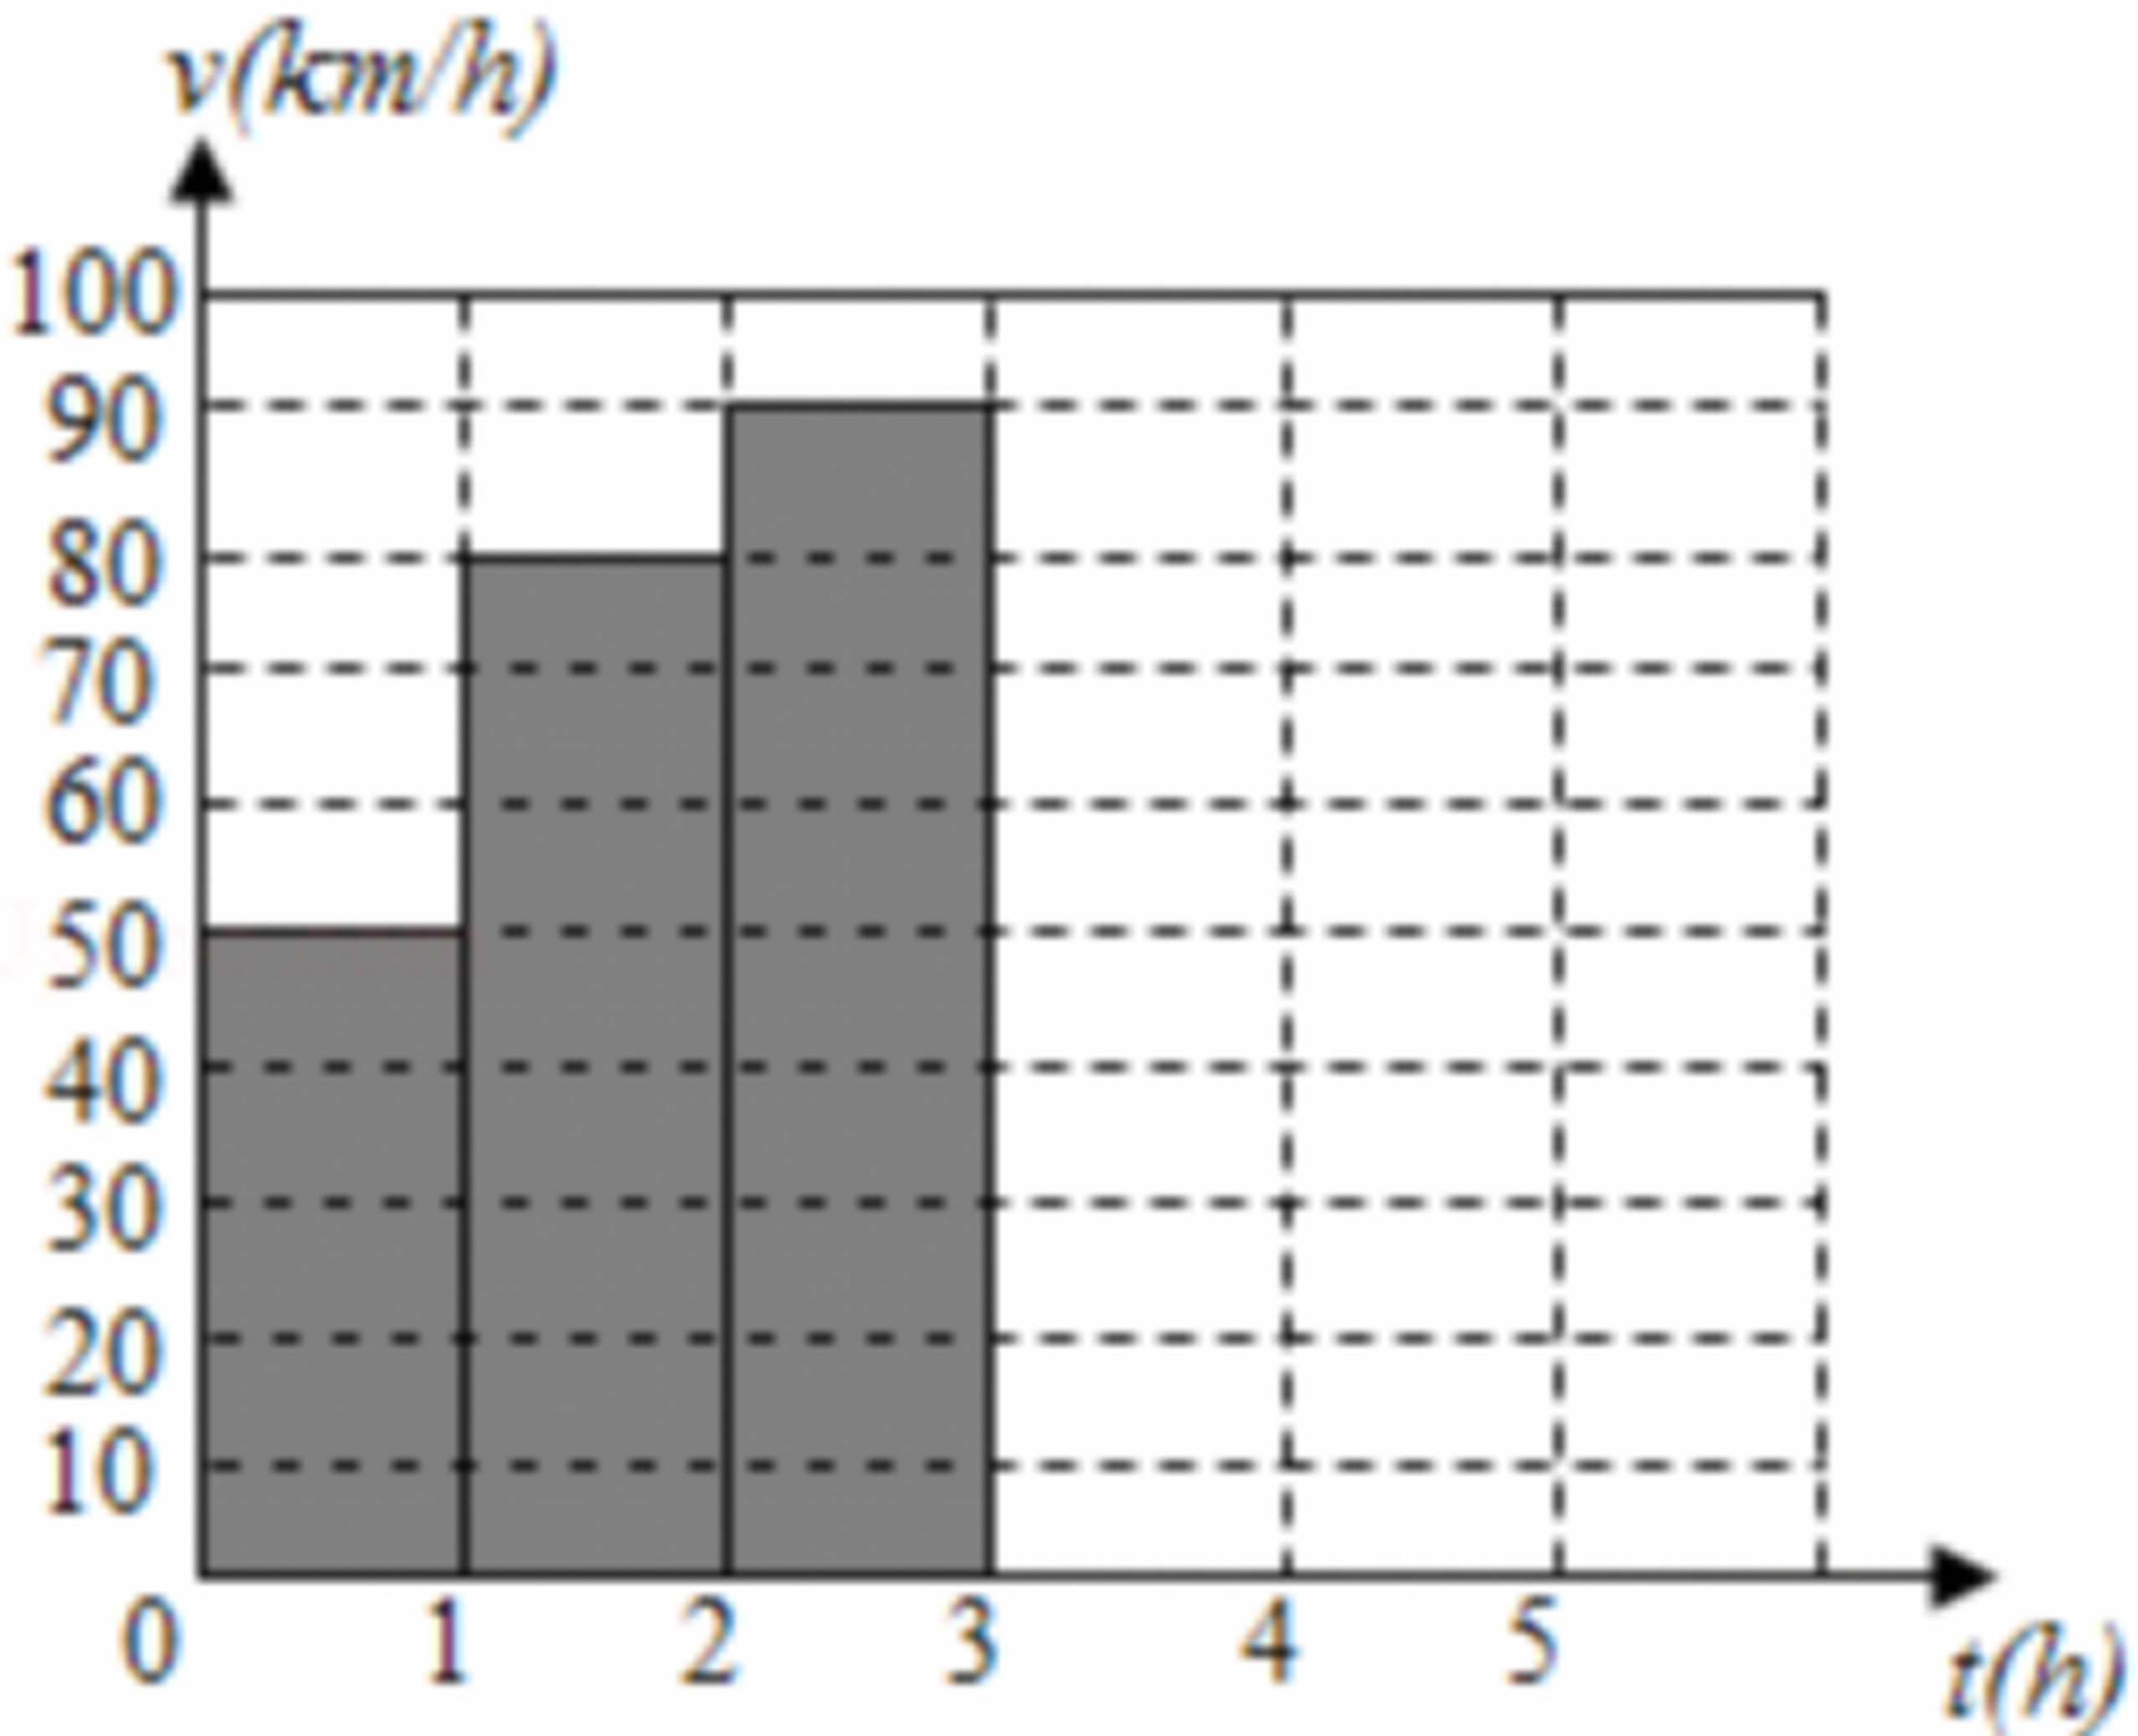
\includegraphics[width=0.52\textwidth]{figures/speed_time_bars.png}
\end{center}

\begin{enumerate}[label=(\arabic*)]
\item 求图中阴影部分的面积，并说明所求面积的实际意义；
\item 假设这辆汽车的里程表在汽车行驶这段路程前的读数为 $2004\,\mathrm{km}$，
试将汽车行驶这段路程时汽车里程表读数 $S$ 表示为时间 $t$ 的函数，
并求出当汽车里程表读数为 $2094\,\mathrm{km}$ 时，汽车行驶了多少时间？
\end{enumerate}

\ifanswer
\solbegin
\stepm{(1)}{由一辆汽车在某段路程中的行驶速度与时间的关系图，}
\step{得阴影部分的面积为 $50\times1+80\times1+90\times1=220$，}
\step{阴影部分的面积表示汽车在 $3$ 小时内行驶的路程为 $220\,\mathrm{km}$.}
\stepm{(2)}{$S=\begin{cases}
50t+2004,&0\leqslant t<1\\
80(t-1)+2054,&1\leqslant t<2\\
90(t-2)+2134,&2\leqslant t\leqslant3
\end{cases}$}
\step{令 $80(t-1)+2054=2094$，解得 $t=1.5$，所以汽车行驶 $1.5$ 小时.}
\solend

\fi

\ansspace[6]

\item 已知集合 $A=\{x\mid x<-2\text{ 或 }x\geqslant3\}$，$U=\R$.

\begin{enumerate}[label=(\arabic*)]
\item 求 $\overline{A}$；
\item 若 $B=\{x\mid mx-1>0\}$，当 $B\sub A$ 时，求实数 $m$ 的取值范围；
\item 若 $B=\{x\mid2m-6\leqslant x\leqslant m+4\}$，当 $B\cap\overline{A}=\varnothing$ 时，
求实数 $m$ 的取值范围.
\end{enumerate}

\ifanswer
\solbegin
\stepm{(1)}{因为集合 $A=\{x\mid x<-2\text{ 或 }x\geqslant3\}$，$U=\R$，
所以 $\overline{A}=\{x\mid-2\leqslant x<3\}$；}
\stepm{(2)}{当 $m=0$ 时，$B=\varnothing$，符合题意，}
\step{当 $m>0$ 时，$B=\left\{x\mid x>\dfrac1m\right\}$，则 $\dfrac1m\geqslant3$，
解得 $0<m\leqslant\dfrac13$，}
\step{当 $m<0$ 时，$B=\left\{x\mid x<\dfrac1m\right\}$，则 $\dfrac1m\leqslant-2$，
解得 $-\dfrac12\leqslant m<0$，}
\step{综上所述，实数 $m$ 的取值范围 $\left[-\dfrac12,\dfrac13\right]$；}
\stepm{(3)}{由题意得 $B=\{x\mid2m-6\leqslant x\leqslant m+4\}$，
$\overline{A}=\{x\mid-2\leqslant x<3\}$，且 $B\cap\overline{A}=\varnothing$，}
\step{当 $B=\varnothing$ 时，$2m-6>m+4$，解得 $m>10$，}
\step{当 $B\neq\varnothing$ 时，则 $\begin{cases}2m-6\leqslant m+4\\ m+4<-2\end{cases}$
或 $\begin{cases}2m-6\leqslant m+4\\ 2m-6\geqslant3\end{cases}$，}
\step{解得 $m<-6$ 或 $\dfrac92\leqslant m\leqslant10$，}
\step{综上所述，实数 $m$ 的取值范围为
$(-\infty,-6)\cup\left[\dfrac92,+\infty\right)$.}
\solend

\fi

\ansspace[8]

\item 在等腰梯形 $ABCD$ 中，$AB=DC=5$，$AD=4$，$BC=10$. 点 $E$ 在下底边 $BC$ 上.
点 $F$ 在腰 $AB$ 上.

\begin{center}
% 图取原卷截图、4× LANCZOS 放大（等腰梯形 $ABCD$ 与线段 $FE$，无辅助线）。
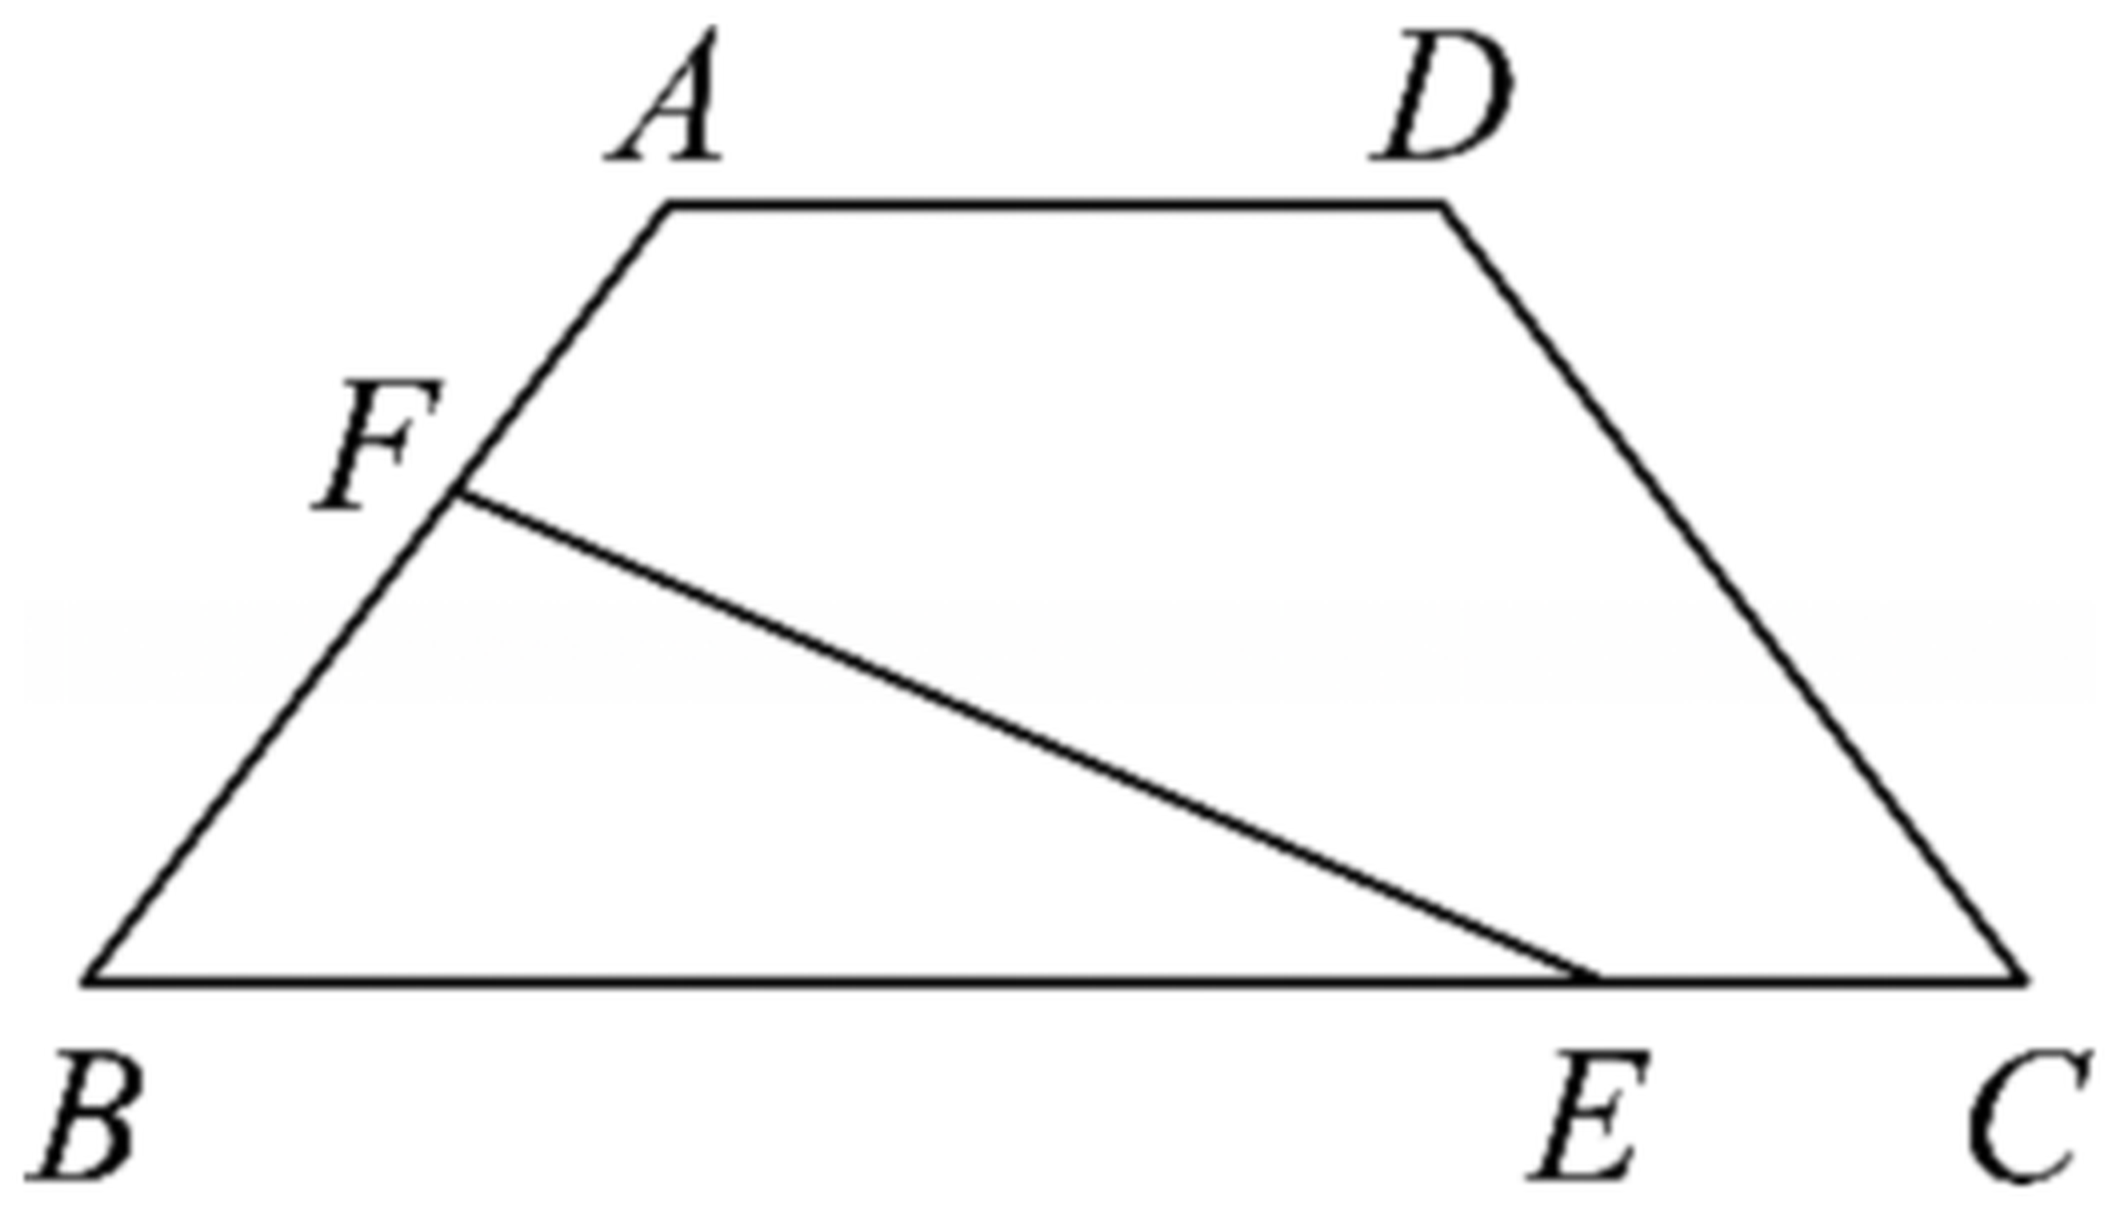
\includegraphics[width=0.46\textwidth]{figures/trapezoid_EF.png}
\end{center}

\begin{enumerate}[label=(\arabic*)]
\item 若 $EF$ 平分等腰梯形 $ABCD$ 的周长，设 $BE$ 长为 $x$，试用含 $x$ 的代数式表示
$\triangle BEF$ 的面积；
\item 是否存在线段 $EF$ 将等腰梯形 $ABCD$ 的周长和面积同时平分？若存在，求出此时 $BE$
的长；若不存在，请说明理由；
\item 是否存在线段 $EF$ 将等腰梯形 $ABCD$ 的周长和面积同时分成 $1:2$ 的两部分？
若存在，求此时 $BE$ 的长；若不存在，请说明理由.
\end{enumerate}

\ifanswer
\solbegin
\stepm{(1)}{过 $A$ 作 $AK\perp BC$ 交 $BC$ 于点 $K$，过 $F$ 作 $FG\perp BC$ 交 $BC$ 于点
$G$，}

\begin{center}
% 图取原卷截图、4× LANCZOS 放大（同梯形，多出虚线 $FG\perp BC$ 与 $AK\perp BC$
% 及两处直角符号；图只在【解析】里出现，故放进 \ifanswer 块）。
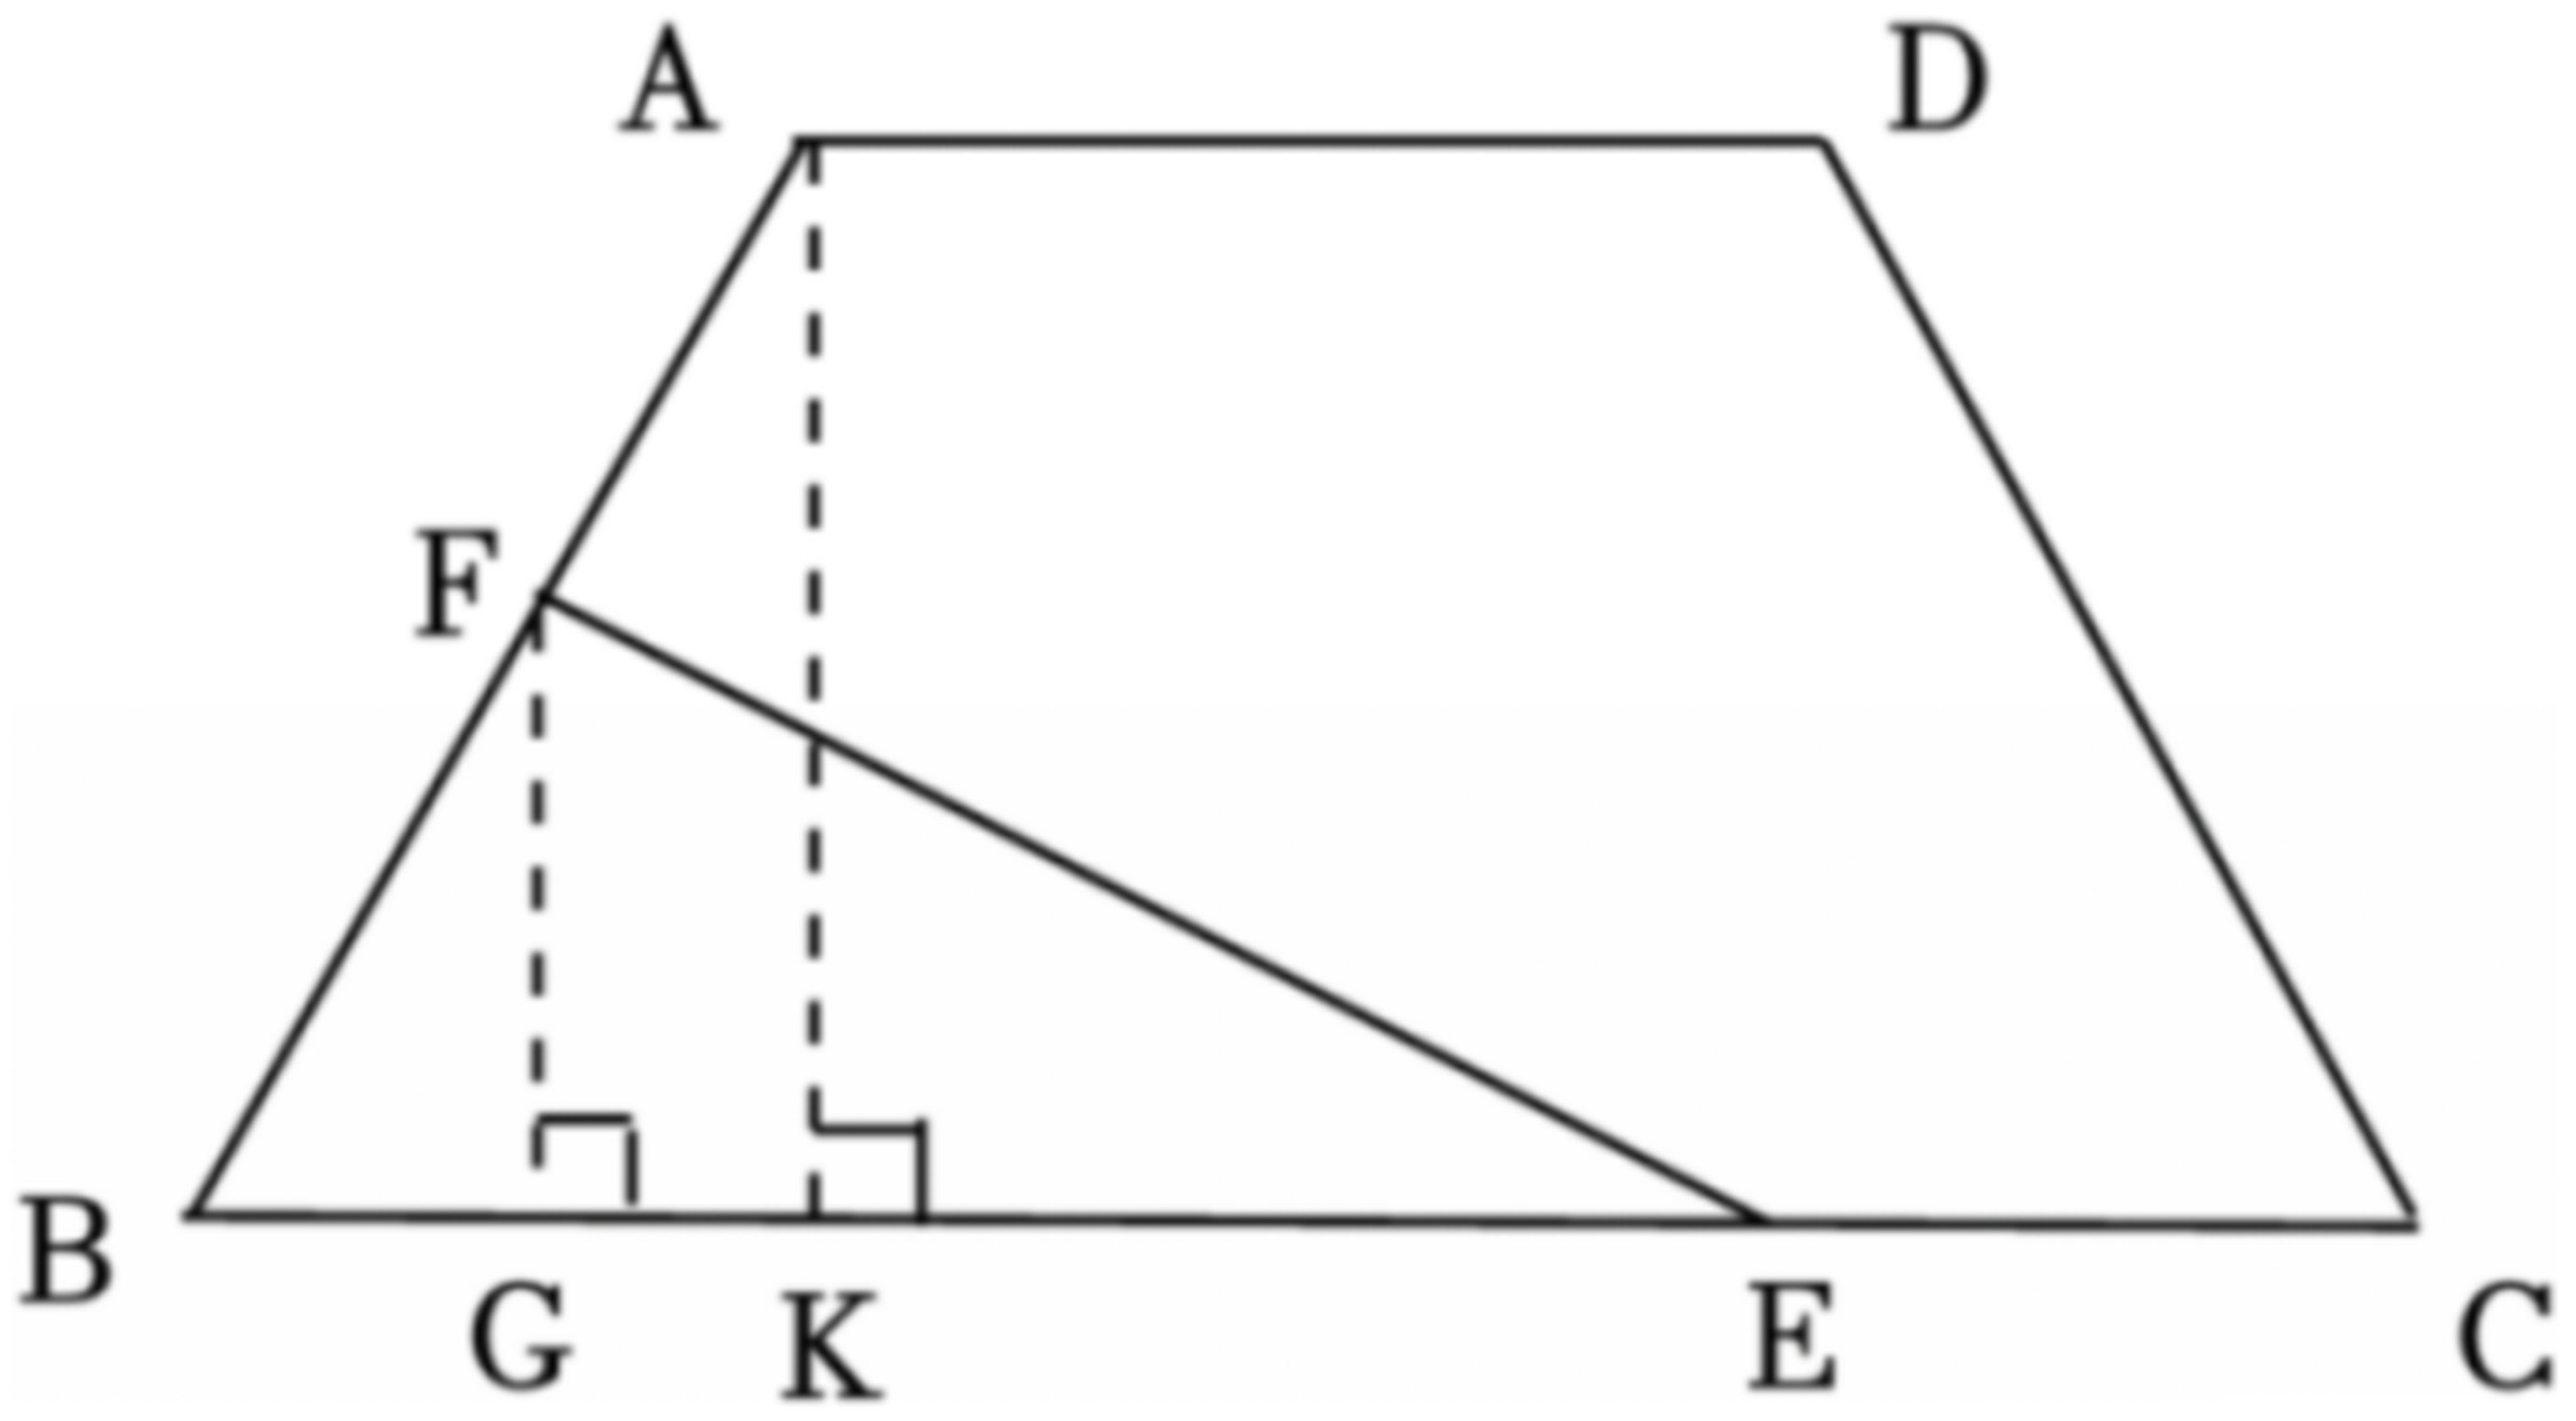
\includegraphics[width=0.62\textwidth]{figures/trapezoid_EF_aux.png}
\end{center}

\step{所以 $BK=\dfrac12\times(BC-AD)=\dfrac12\times(10-4)=3$，}
\step{$AK=\sqrt{AB^2-BK^2}=\sqrt{5^2-3^2}=4$，}
\step{由题意得，梯形 $ABCD$ 周长为 $24$，高为 $4$，面积为 $28$，}
\step{因为 $EF$ 平分等腰梯形 $ABCD$ 的周长，设 $BE$ 长为 $x$，则 $BF=12-x$，}
\step{由 $\begin{cases}0\leqslant12-x\leqslant5\\ 0\leqslant x\leqslant10\end{cases}$，
解得 $7\leqslant x\leqslant10$，}
\step{由题意得 $\triangle BFG\backsim\triangle BAK$，所以 $\dfrac{FG}{AK}=\dfrac{BF}{BA}$，
即 $\dfrac{FG}4=\dfrac{12-x}5$，}
\step{解得 $FG=\dfrac45(12-x)$，}
\step{所以 $S_{\triangle BEF}=\dfrac12BE\cdot FG
=-\dfrac25x^2+\dfrac{24}5x$（$7\leqslant x\leqslant10$）；}
\stepm{(2)}{存在，由 (1) 得 $-\dfrac25x^2+\dfrac{24}5x=\dfrac{28}2$，$x\in[7,10]$，}
\step{即 $x^2-12x+35=0$，解得 $x=7$ 或 $x=5$（舍去），}
\step{所以存在线段 $EF$ 将等腰梯形 $ABCD$ 的周长和面积同时平分，此时 $BE=7$；}
\stepm{(3)}{不存在，}
\step{情况一：$\triangle BEF$ 的面积$:$多边形 $AFECD$ 的面积 $=1:2$，
$(BE+BF):(AF+AD+DC+CE)=1:2$，}
\step{梯形周长的 $\dfrac13$ 是 $\dfrac{24}3=8$，面积的 $\dfrac13$ 是 $\dfrac{28}3$，}
\step{又因为 $BE=x$，所以 $BF=8-x$，}
\step{又因为 $\dfrac{FG}{AK}=\dfrac{BF}{BA}$，即 $\dfrac{FG}4=\dfrac{8-x}5$，
所以 $FG=\dfrac{32-4x}5$，}
\step{所以 $S_{\triangle BEF}=\dfrac12BE\times FG=-\dfrac25x^2+\dfrac{16}5x$，
所以 $\dfrac{28}3=-\dfrac25x^2+\dfrac{16}5x$，}
\step{整理得 $-3x^2+24x-70=0$，此时 $\Delta<0$，无解，故不存在；}
\step{情况二：$\triangle BEF$ 的面积$:$多边形 $AFECD$ 的面积 $=2:1$，
$(BE+BF):(AF+AD+DC+CE)=2:1$，}
\step{梯形周长的 $\dfrac13$ 为 $\dfrac{24}3=8$，面积的 $\dfrac13$ 为 $\dfrac{28}3$，
又 $BE=x$，所以 $BF=16-x$，}
\step{又 $\dfrac{FG}{AK}=\dfrac{BF}{BA}$，即 $\dfrac{FG}4=\dfrac{16-x}5$，
所以 $FG=\dfrac{64-4x}5$，}
\step{所以 $S_{\triangle BEF}=\dfrac12BE\times FG=-\dfrac25x^2+\dfrac{32}5x$，}
\step{所以 $\dfrac{28}3\times2=-\dfrac25x^2+\dfrac{32}5x$，
整理得 $-3x^2+48x-140=0$，}
\step{解得 $x=\dfrac{48+\sqrt{624}}6>10$，$x=\dfrac{48-\sqrt{624}}6<7$，
不符合题意，舍去，故不存在；}
\step{综上所述，不存在线段 $EF$ 将等腰梯形 $ABCD$ 的周长和面积同时分成 $1:2$ 的两部分.}
\solend

\fi

\ansspace[8]

\item 对集合 $\{1,2,\cdots,n\}$ 及其每一个非空子集 $A$，定义一个唯一确定的“交替和”
如下：将 $A$ 中的元素按照递减的次序排列，然后将第一个元素交替地减或加后继的元素所得的
结果，例如，子集 $\{1,2,4,6,9\}$ 的“交替和”是 $9-6+4-2+1=6$，子集 $\{5,6\}$ 的
“交替和”是 $6-5=1$，子集 $\{2\}$ 的交替和是 $2$；定义一个唯一确定的“交替积”如下：
将 $A$ 中的元素按照递减的次序排列，然后将第一个元素交替地除以或乘以后继的数所得的结果，
例如，集合 $\{1,2,4,6,9\}$ 的“交替积”是 $9\div6\times4\div2\times1=3$，
$\{5,6\}$ 的“交替积”是 $6\div5=1.2$，$\{2\}$ 的“交替积”是 $2$.

\begin{enumerate}[label=(\arabic*)]
\item 对于 $\{1,2,3,4,5,6,7,8,9\}$，求其所有子集的“交替和”的总和；
\item 对于 $\{1,2,\cdots,n\}$，求其所有子集的“交替和”的总和；
\item 对于 $\left\{n\mid\dfrac{495}{n+2}\in\N,n\in\Z\right\}$ 求其所有子集的
“交替积”的总和.
\end{enumerate}

\ifanswer
\solbegin
\stepm{(1)}{集合 $\{1,2,3,4,5,6,7,8,9\}$ 的子集中，除去 $\{9\}$ 外还有 $2^9-2$ 个
非空子集，}
\step{把这 $2^9-2$ 个非空子集两两组合后分别计算每一组中“交替和”之和，}
\step{组合原则是设 $A_i=\{9,a_1,a_2,\cdots\}$，$A_i^1=\{a_1,a_2,\cdots\}$，}
\step{集合 $A_i^1$ 的元素为集合 $A_i$ 中去掉 $9$ 的所有元素，把 $A_i$ 和 $A_i^1$
结合为一组，}
\step{显然，每组的“交替和”的和为 $9$，共有 $\dfrac{2^9-2}2$ 组，}
\step{所以，所有“交替和”之和应该为 $\dfrac{9(2^9-2)}2+9=2304$；}
\stepm{(2)}{集合 $\{1,2,\cdots,n\}$ 的子集中，除去 $\{n\}$ 外还有 $2^n-2$ 个非空子集，}
\step{把这 $2^n-2$ 个非空子集两两组合后分别计算每一组中“交替和”之和，}
\step{组合原则是设 $A_i=\{n,a_1,a_2,\cdots\}$，$A_i^1=\{a_1,a_2,\cdots\}$，}
\step{集合 $A_i^1$ 的元素为集合 $A_i$ 中去掉 $n$ 的所有元素，把 $A_i$ 和 $A_i^1$
结合为一组，}
\step{显然，每组的“交替和”的和为 $n$，共有 $\dfrac{2^n-2}2$ 组，}
% 注：下一行分子原卷印作花括号（其余同类处皆用圆括号），照抄未改，见文件头“原卷存疑”③。
\step{所以，所有“交替和”之和应该为 $\dfrac{n\{2^n-2\}}2+n=n\cdot2^{n-1}$；}
\stepm{(3)}{集合 $\left\{n\mid\dfrac{495}{n+2}\in\N,n\in\Z\right\}
=\{493,163,97,53,43,31,13,9,7,3,1,-1\}$，}
\step{其中除去 $\{-1\}$ 外还有 $2^{12}-2$ 个非空子集，}
% 注：下一行原卷把“把这”重复印了一次（“把这把这”），照抄未改，见文件头“原卷存疑”②。
\step{把这把这 $2^{12}-2$ 个非空子集两两组合后分别计算每一组中“交替积”之和，}
\step{组合原则是设 $A_j=\{-1,a_1,a_2,\cdots\}$，$A_j^1=\{a_1,a_2,\cdots\}$，}
\step{集合 $A_j^1$ 的元素为集合 $A_j$ 中去掉 $-1$ 的所有元素，把 $A_j$ 和 $A_j^1$
结合为一组，}
\step{显然，每组的“交替积”的和为 $0$，共有 $\dfrac{2^{12}-2}2$ 组，}
\step{所以，所有“交替积”之和应该为 $\dfrac{2^{12}-2}2\times0-1=-1$.}
\solend

\fi

\ansspace*[10]

\end{enumerate}

\end{document}
"
%
% 原始材料是微信公众号图文（公众号“魔都数学加油站”连载“27学年高一 30”，2026-09-23 发布，
% 原文标题“27学年高一30——2026-2027年上海市南洋模范中学高一上开学考”），
% 正文为 11 张 PNG 页。**同一篇里各页分辨率不一致**——第 2、3、9、10 页 4762×6735，
% 其余七页 2560×3620（已逐页打开确认，非下载缺档），取的是 mmbiz.qpic.cn/<hash>/0 的原图档。
% 原文本身就是一份**讲评版**：填空第 3—7 题下方印【答案】，第 8—12 题与其后各题印【解析】。
% 试题文字、答案与解析均照原卷录入，未改内容。卷面的粉色斜水印属水印，未录入。
%
% 卷首标题：原卷印作“2026-2027 年南洋模范中学高一上开学考”（公众号标题里的“上海市”
% 三字卷面标题行没有，本稿照卷面），年份区间按全稿惯例排 en dash，前缀照原卷保留“年”。
%
% 与原卷的排版差异（均已在 README“说明”中交代）：
%   ① 原文自**第 3 题**起（第 1、2 题未在该文中发布），故本稿题号亦自 3 起；
%   ② 原卷本就印有“一、填空题”“二、选择题”“三、解答题”三节标题，本稿照原卷分节，
%      只把标题改排成全稿统一的“大节标题”样式；
%   ③ 原卷填空第 3—7 题只印【答案】行、第 8 题起印【解析】（选择题答案写在解析末句
%      “故选 D／B”里），本稿统一改为试卷版隐去、答案版以 \ans{}／\ifanswer 块给出，
%      两版彻底分离；
%   ④ 子集符号原卷两种并用：第 7 题题干两处、第 19(2) 题作带下划线的 $\subseteq$，
%      第 17(2) 题解析作真包含的 $\subset$，本稿分别照录为 $\sub$ 与 $\subset$；
%   ⑤ 补集符号原卷一律作**上横线**（$\overline{A}$、$\overline{B}$），本稿照录；
%   ⑥ 原卷的实数集 R 一律作斜体（第 4 题、第 17 题与第 19 题题干的 $U=R$），
%      第 21(3) 题的自然数集与整数集作**粗体** $\mathbf{N}$、$\mathbf{Z}$，
%      本稿按全稿惯例统一写作 $\R$、$\N$、$\Z$；
%   ⑦ 原卷填空的横线约两个字宽，本稿按全稿惯例统一排 \blankline[4.4em]；
%   ⑧ 原卷未印副标题，本稿按全稿惯例补出副标题“集合与常用逻辑用语”——但本卷是开学考，
%      范围不止这一章：第 18 题是速度—时间图象题、第 20 题是等腰梯形的周长/面积平分问题，
%      副标题只标了主章节（见文末“高一30 专记”）；
%   ⑨ 第 13、14、18、20 题的图印在题干右侧、第 16 题的三幅图印在【解析】里的下一页顶部、
%      第 20 题【解析】另有一张带辅助线的图，本稿一律移至题干或解析之后；
%      图取原卷截图、4× LANCZOS 放大（见各 \includegraphics 前的注释）。
%
% 原卷存疑三处（均照抄原卷、未改，见源码中该处上方注释）：
%   ① 第 10 题【解析】验证“破晓集”时写的是 $\notin A$、$\in A$（如“$-2-2=-4\notin A$”），
%      但该处讨论的集合原题设里叫 $P$，同题②的“$x+y=2(k_1+k_2)\in A$”亦然——
%      本稿照抄未改（按文意应为 $P$）；
%   ② 第 21 题【解析】(3) 有“把这把这 $2^{12}-2$ 个非空子集”（“把这”重复印了一次）；
%   ③ 同题 (2) 的结论式分子原卷印作花括号 $\dfrac{n\{2^n-2\}}{2}$（其余同类处皆用圆括号）。

\documentclass[a4paper,11pt]{article}
\usepackage{common}

\begin{document}

\examtitlest[3]{2026--2027 年南洋模范中学高一上开学考}{集合与常用逻辑用语}

\bigsec{一、填空题}

\begin{enumerate}
\setcounter{enumi}{2}

\item 若集合 $A=\{x\mid x^2-2kx+7k=0\}$ 有且仅有三个真子集，则 $k$ 的取值范围是
\blankline[4.4em].

\ans{$(-\infty,0)\cup(7,+\infty)$}

\item “存在 $x\in\R$，使得 $x^2+2x+5=0$”的否定形式是 \blankline[4.4em].

\ans{对任何 $x\in\R$，都有 $x^2+2x+5\neq0$}

\item 下列命题中，$p$ 是 $q$ 的必要非充分条件的是 \blankline[4.4em].

① $p:x>2$ 且 $y>3$，$q:x+y>5$；

② $p$：四边形的四个角都相等，$q$：四边形是正方形.

\ans{②}

\item 若“条件 $\alpha:2\leqslant x\leqslant4$”是“条件 $\beta:3m-1\leqslant x\leqslant-m$”的
充分非必要条件，则 $m$ 的取值范围是 \blankline[4.4em].

\ans{$(-\infty,-4]$}

\item 满足 $\{1\}\sub M\sub\{1,2,4,5\}$ 的集合 $M$ 的个数为 \blankline[4.4em] 个.

\ans{$8$}

\item 已知集合 $A=\{1,2\}$，集合 $B=\{x\mid ax=6\}$，若 $A\cup B=A$，则 $a$ 的所有取值
构成的集合为 \blankline[4.4em].

\ifanswer
\solbegin
\step{因为 $A\cup B=A$，所以 $B\sub A$，}
\step{当 $a=0$ 时，$B=\varnothing$，满足 $B\sub A$；}
\step{当 $a\neq0$ 时，$B=\left\{\dfrac6a\right\}$，则 $\dfrac6a=1$ 或 $\dfrac6a=2$，
解得 $a=6$ 或 $a=3$，}
\step{综上所述，$a$ 的所有取值构成的集合为 $\{0,3,6\}$.}
\solend

\fi

\item 对于集合 $M$、$N$，定义 $M-N=\{x\mid x\in M\text{ 且 }x\notin N\}$，
$M\oplus N=(M-N)\cup(N-M)$，设 $A=\{y\mid y=|x|,x\in\R\}$，
$B=\{y\mid y=-(x-1)^2+2,x\in\R\}$，则 $A\oplus B=$ \blankline[4.4em].

\ifanswer
\solbegin
\step{由已知 $A=[0,+\infty)$，$B=(-\infty,2]$，}
\step{由于 $A-B=(2,+\infty)$，$B-A=(-\infty,0)$，}
\step{故 $A\oplus B=(A-B)\cup(B-A)=(-\infty,0)\cup(2,+\infty)$.}
\solend

\fi

\item 设 $P$ 为非空实数集满足：对任意给定的 $x$、$y\in P$（$x$、$y$ 可以相同），都有
$x+y\in P$，$x-y\in P$，$xy\in P$，则称 $P$ 为破晓集. 关于破晓集有下列结论：
①集合 $P=\{-2,-1,0,1,2\}$ 为破晓集；②集合 $P=\{x\mid x=2n,n\in\Z\}$ 为破晓集；
③若集合 $P_1$、$P_2$ 为破晓集，则 $P_1\cup P_2$ 为破晓集；④若集合 $P$ 为破晓集，
则一定有 $0\in P$；⑤若集合 $P_1$、$P_2$ 为破晓集，则 $P_1\cap P_2$ 为破晓集；
其中正确结论的序号是 \blankline[4.4em].

\ifanswer
\solbegin
% 注：以下几步原卷把该集合记作 $A$（题设里叫 $P$），照抄未改，见文件头“原卷存疑”①。
\step{对于①：$-2-2=-4\notin A$，故集合 $P=\{-2,-1,0,1,2\}$ 不为破晓集，故①错误；}
\step{②设 $x$、$y\in A$，则 $x=2k_1$，$y=2k_2$，且 $k_1$、$k_2\in\Z$，}
\step{故 $x+y=2(k_1+k_2)\in A$，$x-y=2(k_1-k_2)\in A$，$xy=4k_1k_2\in A$，}
\step{故集合 $P=\{x\mid x=2n,n\in\Z\}$ 为破晓集，故②正确；}
\step{③若集合 $P_1$、$P_2$ 为破晓集，设 $P_1=\{x\mid x=2k,k\in\Z\}$，
$P_2=\{x\mid x=3k,k\in\Z\}$，}
\step{但是 $P_1\cup P_2$ 不为破晓集，如 $x=2$，$y=3$ 时，$x+y=5$，
故 $5\notin(P_1\cup P_2)$，故③错误；}
\step{④若集合 $P$ 为破晓集，则取 $x=y$，$x-y=0\in A$，则一定有 $0\in P$，故④正确.}
\step{⑤正确；}
\step{故正确的是②④⑤.}
\solend

\fi

\item 已知集合 $M$ 的元素均为正整数，定义集合 $M$ 的“变项和”为：将 $M$ 中每个元素 $m$
都乘以 $(-1)^m$ 后再求和. 若集合 $A=\{n\mid1\leqslant n\leqslant10,n\in\N\}$，则集合 $A$
的所有非空子集的“变项和”的总和为 \blankline[4.4em].

\ifanswer
\solbegin
\step{$A$ 集合的所有非空子集中，每个元素出现的次数都是
$(2^{10}-1)-(2^9-1)=2^9$，}
\step{则集合 $A$ 的所有非空子集的“变项和”的总和为
$1\times(-1)^1\times2^9+2\times(-1)^2\times2^9+\cdots+10\times(-1)^{10}\times2^9$}
\step{$=(-1+2-3+4-\cdots-9+10)\times2^9=5\times2^9=2560$.}
\solend

\fi

\item 已知集合 $A=[t,t+1]\cup[t+4,t+9]$，$0\notin A$，存在正数 $\lambda$，使得对任意
$a\in A$，都有 $\dfrac\lambda a\in A$，则 $t$ 的值是 \blankline[4.4em].

\ifanswer
\solbegin
\step{当 $t>0$ 时，当 $a\in[t,t+1]$ 时，$\dfrac\lambda a\in[t+4,t+9]$，}
\step{当 $a\in[t+4,t+9]$ 时，$\dfrac\lambda a\in[t,t+1]$，}
\step{即当 $a=t$ 时，$\dfrac\lambda a\leqslant t+9$；当 $a=t+9$ 时，
$\dfrac\lambda a\geqslant t$，即 $\lambda=t(t+9)$；}
\step{当 $a=t+1$ 时，$\dfrac\lambda a\geqslant t+4$，当 $a=t+4$ 时，
$\dfrac\lambda a\leqslant t+1$，即 $\lambda=(t+1)(t+4)$，}
\step{所以 $t(t+9)=(t+1)(t+4)$，解得 $t=1$.}
\step{当 $t+1<0<t+4$ 时，当 $a\in[t,t+1]$ 时，$\dfrac\lambda a\in[t,t+1]$.}
\step{当 $a\in[t+4,t+9]$ 时，则 $\dfrac\lambda a\in[t+4,t+9]$，}
\step{即当 $a=t$ 时，$\dfrac\lambda a\leqslant t+1$，当 $a=t+1$ 时，
$\dfrac\lambda a\geqslant t$，即 $\lambda=t(t+1)$，}
\step{即当 $a=t+4$ 时，$\dfrac\lambda a\leqslant t+9$，当 $a=t+9$ 时，
$\dfrac\lambda a\geqslant t+4$，即 $\lambda=(t+4)(t+9)$，}
\step{所以 $t(t+1)=(t+4)(t+9)$，解得 $t=-3$.}
\step{当 $t+9<0$ 时，同理可得无解.}
\step{综上，$t$ 的值为 $1$ 或 $-3$.}
\solend

\fi

\end{enumerate}

\bigsec{二、选择题}

\begin{enumerate}
\setcounter{enumi}{12}

% 这道题是“题干 + 图 + 选项”约 6cm 的一整块，页末放不下就会被拆开（切页审计的 A 类），
% 故在题前先量一次页高：不够就把整道题干连图带选项一起挪到次页。
\needvspace{6.5cm}
\item 设 $U=\{1,2,3,4,5\}$，$A$、$B$ 都是 $U$ 的子集，且 $A\cap B=\{5\}$，
$\overline{A}\cap B=\{4\}$，$\overline{A}\cap\overline{B}=\{1,2\}$，
则以下四个判断中正确的是\mbox{（\quad）}

\begin{center}
% 图取原卷截图、4× LANCZOS 放大（原卷把图印在题干右侧，本稿移至此处，见文件头⑨）。
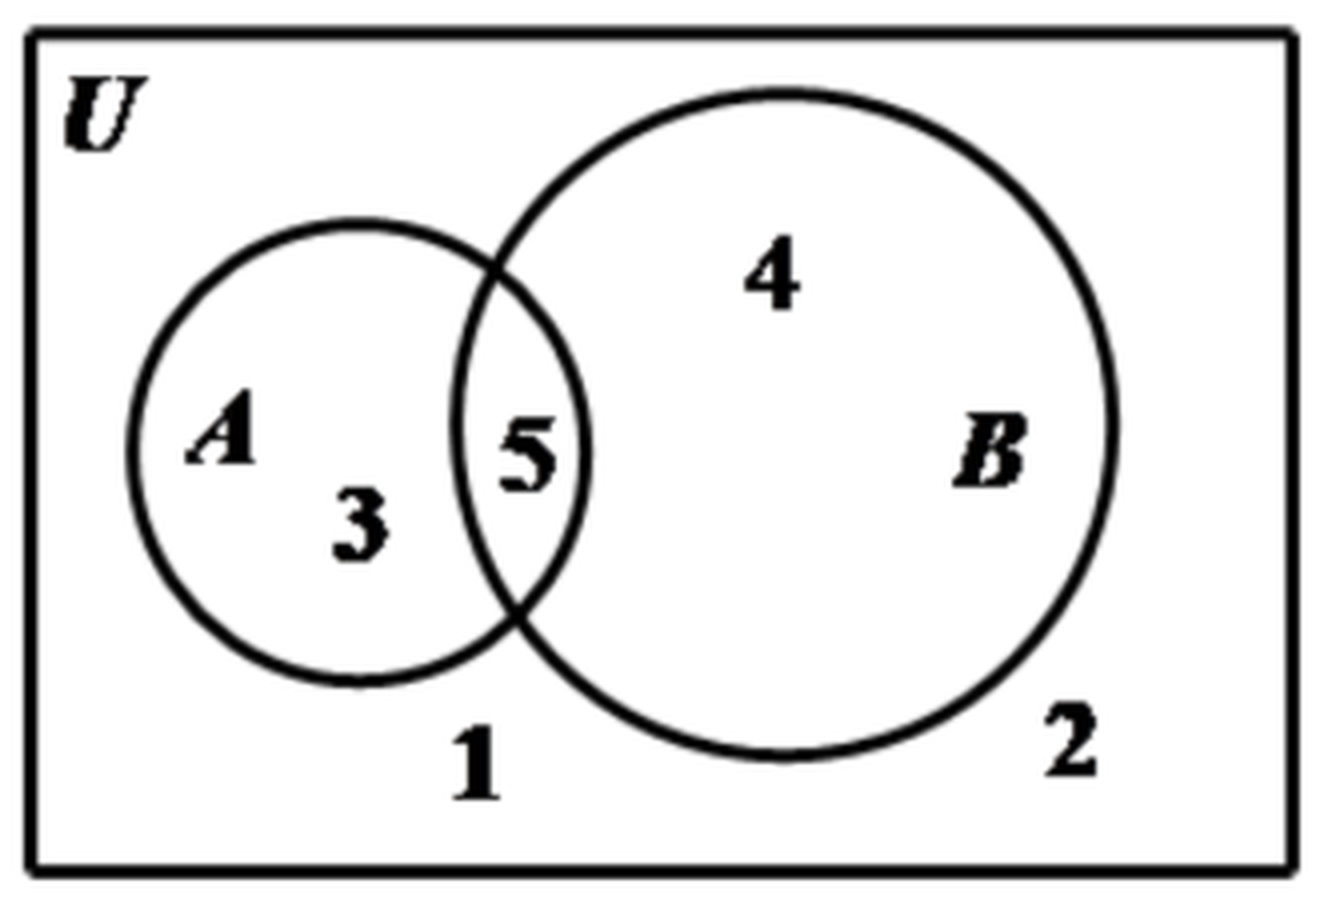
\includegraphics[width=0.28\textwidth]{figures/venn_U5_AB.png}
\end{center}

\keepwithprev
A. $3\notin A$ 且 $3\notin B$\qquad\qquad B. $3\in A$ 且 $3\in B$

C. $3\notin A$ 且 $3\in B$\qquad\qquad D. $3\in A$ 且 $3\notin B$

\ans{$D$}

\ifanswer
\solbegin
\step{画出韦恩图，得 $A=\{5,3\}$，$B=\{5,4\}$，}
\step{则 $3\in A$ 且 $3\notin B$. 故选 $D$.}
\solend

\fi

% 同第 13 题：整块（题干 + 图 + 选项）在答案版还要再挂【答案】【解析】，页末更易被拆开。
\needvspace{7.5cm}
\item 如图表示图形阴影部分的是\mbox{（\quad）}

\begin{center}
% 图取原卷截图、4× LANCZOS 放大（三圆 $A$、$B$、$C$，阴影为整个 $A$ 圆加 $B\cap C$）。
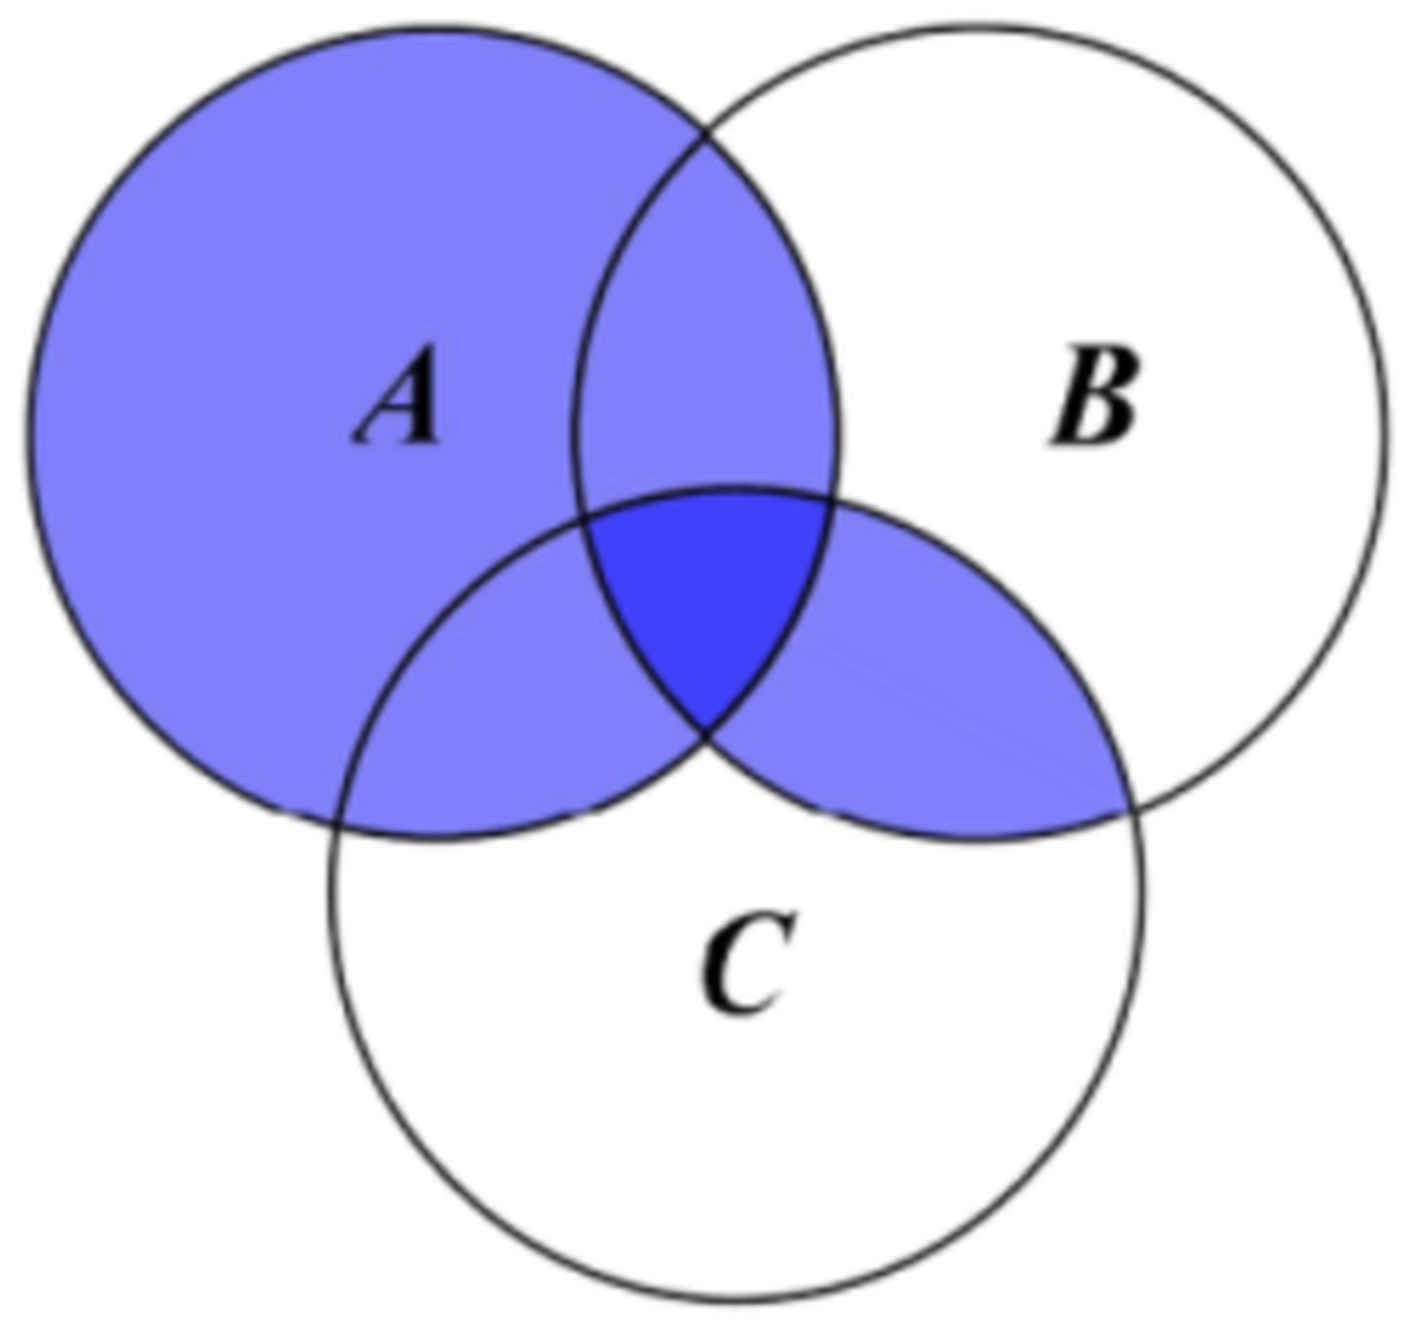
\includegraphics[width=0.30\textwidth]{figures/venn_A_union_BC.png}
\end{center}

\keepwithprev
A. $(A\cup C)\cap(B\cup C)$\qquad\qquad B. $(A\cup B)\cap(A\cup C)$

C. $(A\cup B)\cap(B\cup C)$\qquad\qquad D. $(A\cup B)\cap C$

\ans{$B$}

\ifanswer
\solbegin
\step{图中阴影部分表示元素满足是 $A$ 中的元素，或者是 $B$ 与 $C$ 的公共元素，}
\step{故可以表示为 $A\cup(B\cap C)$，也可以表示为 $(A\cup B)\cap(A\cup C)$.
故选 $B$.}
\solend

\fi

\item 设集合 $M=\left\{x\mid m\leqslant x\leqslant m+\dfrac34\right\}$，
$N=\left\{x\mid n-\dfrac13\leqslant x\leqslant n\right\}$，且 $M$、$N$ 都是集合
$\{x\mid0\leqslant x\leqslant1\}$ 的子集，如果把 $b-a$ 叫做集合
$\{x\mid a\leqslant x\leqslant b\}$ 的“长度”，那么集合 $M\cap N$ 的“长度”的
最小值是\mbox{（\quad）}

\keepwithprev
A. $\dfrac23$\qquad B. $\dfrac1{12}$\qquad C. $\dfrac13$\qquad D. $\dfrac5{12}$

\ans{$B$}

\ifanswer
\solbegin
\step{$M$ 的长度为 $\dfrac34$，$N$ 的长度为 $\dfrac13$，}
\step{当集合 $M\cap N$ 的长度的最小值时，$M$ 与 $N$ 应分别在区间 $[0,1]$ 的左右两端，}
\step{故 $M\cap N$ 的长度的最小值是 $\dfrac34+\dfrac13-1=\dfrac1{12}$，故选 $B$.}
\solend

\fi

\item 定义集合运算 $A-B=\{x\mid x\in A\text{ 且 }x\notin B\}$ 称为集合 $A$ 与集合 $B$ 的
差集；定义集合运算 $A\Delta B=(A-B)\cup(B-A)$ 称为集合 $A$ 与集合 $B$ 的对称差，
有以下 $4$ 个等式：① $A\Delta B=B\Delta A$；② $(A\Delta B)\Delta C=A\Delta(B\Delta C)$；
③ $A\cap(B\Delta C)=(A\cap B)\Delta(A\cap C)$；
④ $A\cup(B\Delta C)=(A\cup B)\Delta(A\cup C)$，
则 $4$ 个等式中恒成立的是\mbox{（\quad）}

\keepwithprev
A. ①②\qquad B. ①②③\qquad C. ①②④\qquad D. ①②③④

\ans{$B$}

\ifanswer
\solbegin
\step{对于①，由 $B\Delta A=(B-A)\cup(A-B)=(A-B)\cup(B-A)=A\Delta B$，
所以①正确；}
\step{对于②，由 $A-B=\{x\mid x\in A\text{ 且 }x\notin B\}
=\{x\mid x\in A,x\notin(A\cap B)\}=A-(A\cap B)$，}
\step{同理可得 $B-A=B-(A\cap B)$，}
\step{则 $A\Delta B=(A-B)\cup(B-A)=(A\cup B)-(A\cap B)$，}
\step{所以 $(A\Delta B)\Delta C=(A\Delta B)\cup C-(A\Delta B)\cap C$，}
\step{所以表示的集合为图（1）中阴影部分所表示的集合，如图所示，}
\step{同理 $A\Delta(B\Delta C)=A\cup(B\Delta C)-A\cap(B\Delta C)$，
也表示图（1）中阴影部分所表示的集合，}
\step{所以 $(A\Delta B)\Delta C=A\Delta(B\Delta C)$，所以②正确；}

\begin{center}
% 图取原卷截图、4× LANCZOS 放大（原卷印在下一页顶部，共三幅三圆韦恩图：
% 图（1）一幅、图（2）左右两幅，图（2）两幅下方各有一行式子标注）。
% 图只在【解析】里出现，故放进 \ifanswer 块，试卷版不排。
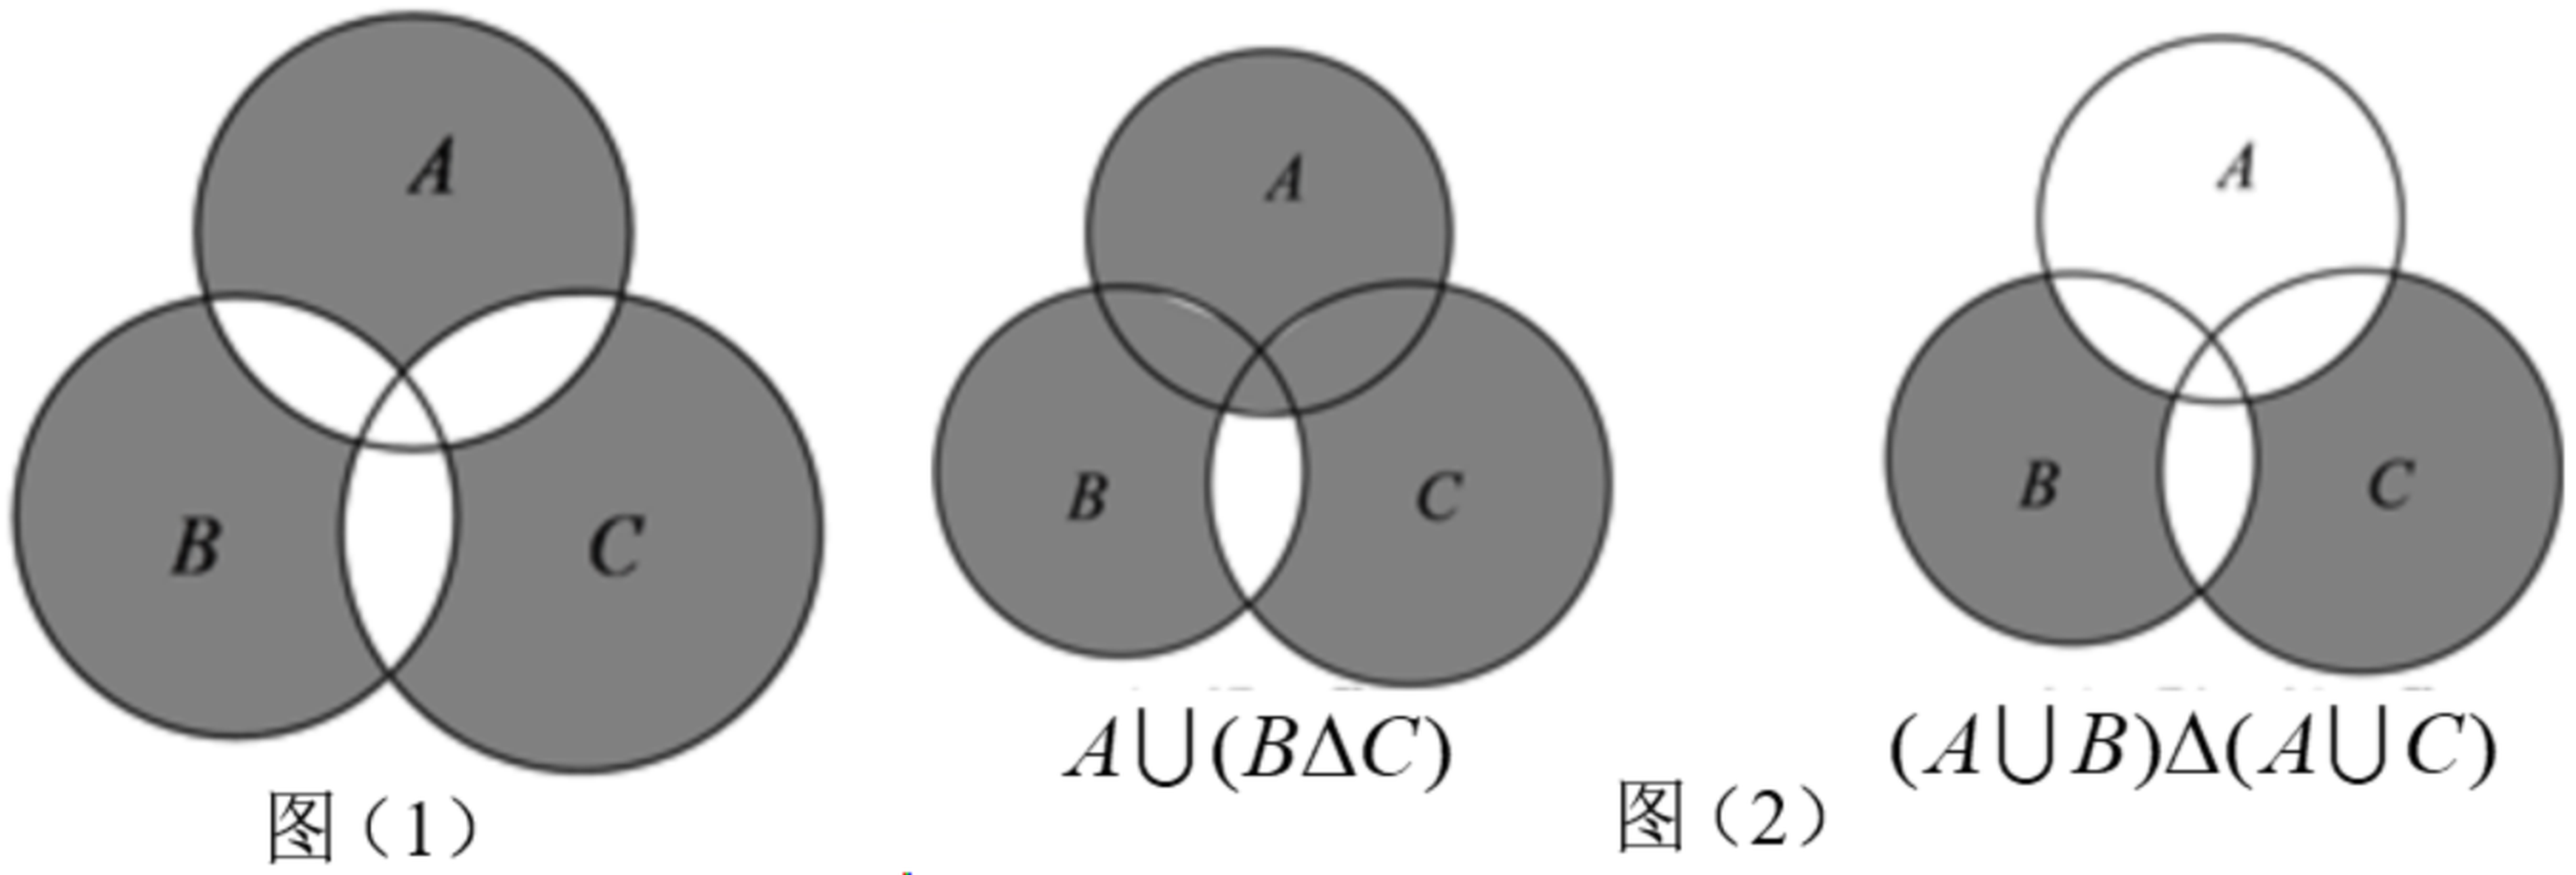
\includegraphics[width=0.86\textwidth]{figures/venn_symdiff3.png}
\end{center}

\step{对于③，由 $A\cap(B\Delta C)=A\cap(B\cup C-B\cap C)
=A\cap(B\cup C)-A\cap(B\cap C)$}
\step{$=(A\cap B)\cup(A\cap C)-(A\cap B)\cap(A\cap C)=(A\cap B)\Delta(A\cap C)$，
所以③正确；}
\step{对于④，如图（2）所示，$A\cup(B\Delta C)\neq(A\cup B)\Delta(A\cup C)$，
所以④错误.}
\step{故选 $B$.}
\solend

\fi

\end{enumerate}

\bigsec{三、解答题}

\begin{enumerate}
\setcounter{enumi}{16}

\item 已知集合 $M=\{x\mid a-1\leqslant x\leqslant2a+3\}$，$P=\{x\mid-2<x\leqslant4\}$，
全集 $U=\R$.

\begin{enumerate}[label=(\arabic*)]
\item 当 $a=2$ 时，求 $M\cap P$；
\item 若 $x\in P$ 是 $x\in M$ 的必要不充分条件，求实数 $a$ 的取值范围.
\end{enumerate}

\ifanswer
\solbegin
\stepm{(1)}{当 $a=2$ 时，集合 $M=\{x\mid1\leqslant x\leqslant7\}$，}
\step{所以 $M\cap P=\{x\mid1\leqslant x\leqslant4\}$；}
\stepm{(2)}{因为 $x\in P$ 是 $x\in M$ 的必要不充分条件，所以 $M\subset P$，}
\step{当 $M=\varnothing$ 时，$a-1>2a+3$，解得 $a<-4$，}
\step{当 $M\neq\varnothing$ 时，则
$\begin{cases}a-1\leqslant2a+3\\ a-1>-2\\ 2a+3\leqslant4\end{cases}$，
解得 $-1<a\leqslant\dfrac12$，}
\step{综上所述，实数 $a$ 的取值范围为
$(-\infty,-4)\cup\left(-1,\dfrac12\right]$.}
\solend

\fi

\ansspace[6]

\item 一辆汽车在某段路程中的行驶速度与时间的关系如图：

\begin{center}
% 图取原卷截图、4× LANCZOS 放大（速度—时间图：纵轴 $v/(\mathrm{km/h})$、
% 横轴 $t(\mathrm{h})$，$t\in[0,1]$、$[1,2]$、$[2,3]$ 三段矩形条高 50、80、90）。
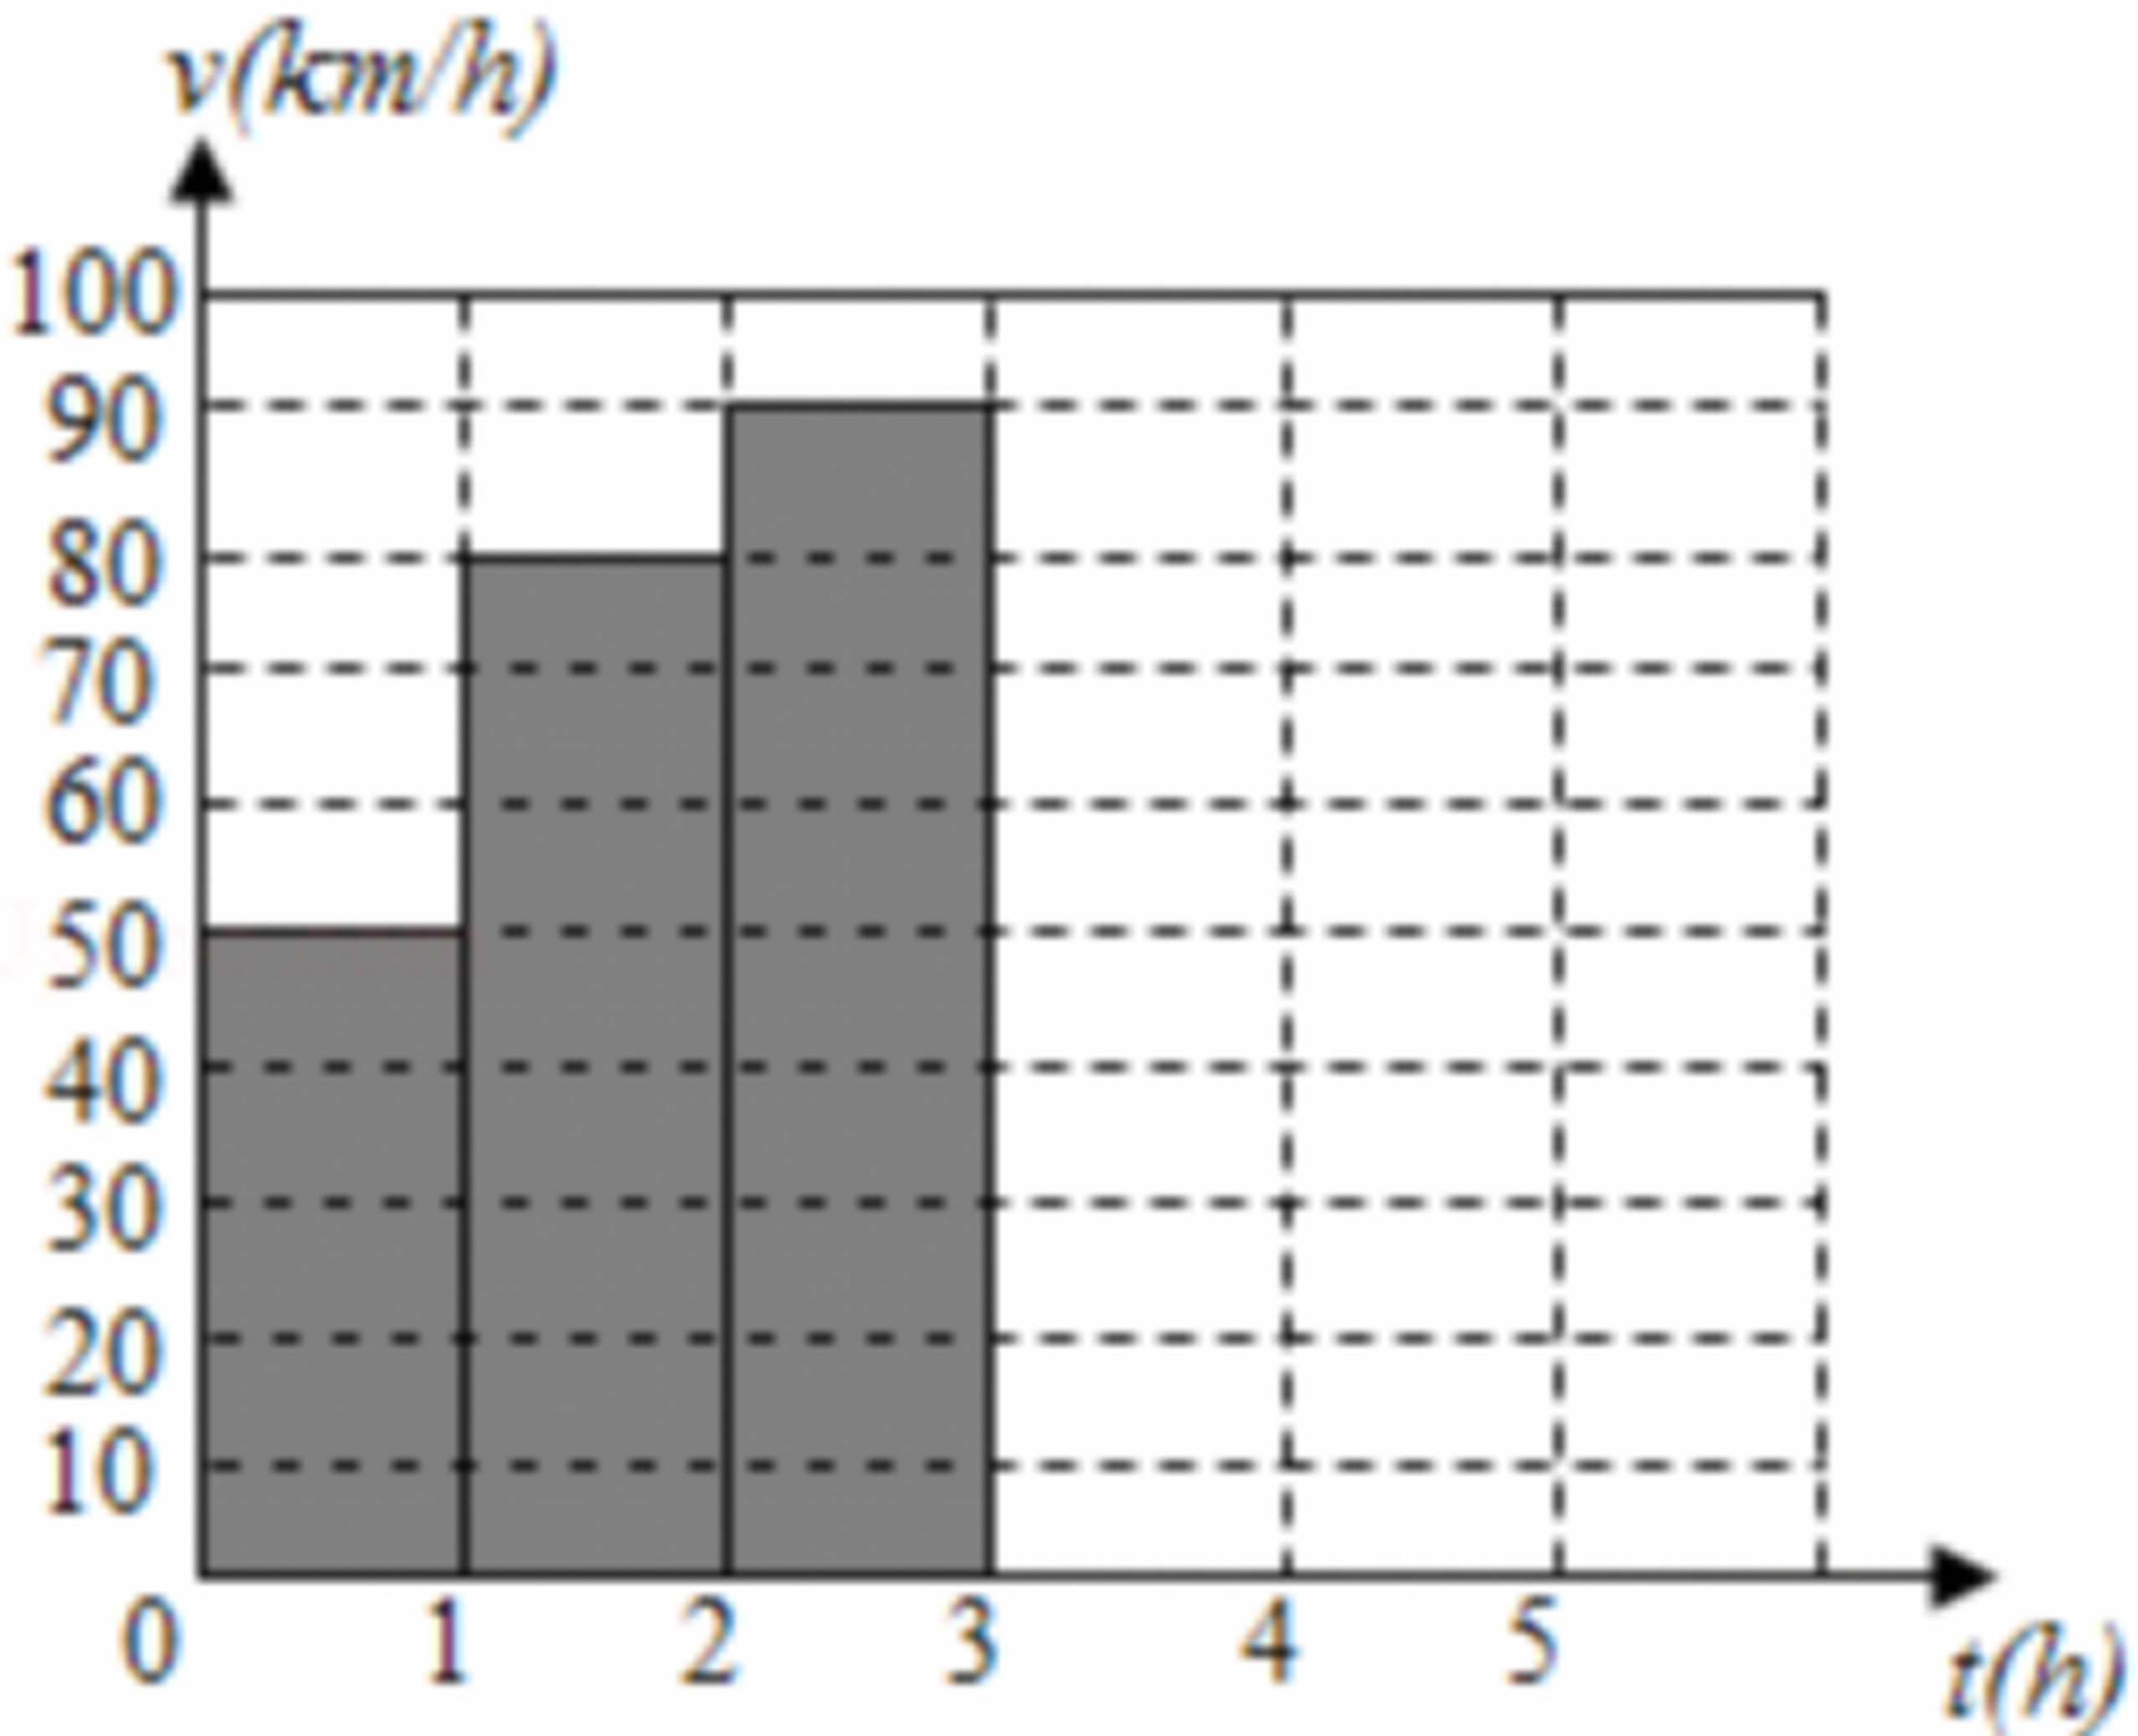
\includegraphics[width=0.52\textwidth]{figures/speed_time_bars.png}
\end{center}

\begin{enumerate}[label=(\arabic*)]
\item 求图中阴影部分的面积，并说明所求面积的实际意义；
\item 假设这辆汽车的里程表在汽车行驶这段路程前的读数为 $2004\,\mathrm{km}$，
试将汽车行驶这段路程时汽车里程表读数 $S$ 表示为时间 $t$ 的函数，
并求出当汽车里程表读数为 $2094\,\mathrm{km}$ 时，汽车行驶了多少时间？
\end{enumerate}

\ifanswer
\solbegin
\stepm{(1)}{由一辆汽车在某段路程中的行驶速度与时间的关系图，}
\step{得阴影部分的面积为 $50\times1+80\times1+90\times1=220$，}
\step{阴影部分的面积表示汽车在 $3$ 小时内行驶的路程为 $220\,\mathrm{km}$.}
\stepm{(2)}{$S=\begin{cases}
50t+2004,&0\leqslant t<1\\
80(t-1)+2054,&1\leqslant t<2\\
90(t-2)+2134,&2\leqslant t\leqslant3
\end{cases}$}
\step{令 $80(t-1)+2054=2094$，解得 $t=1.5$，所以汽车行驶 $1.5$ 小时.}
\solend

\fi

\ansspace[6]

\item 已知集合 $A=\{x\mid x<-2\text{ 或 }x\geqslant3\}$，$U=\R$.

\begin{enumerate}[label=(\arabic*)]
\item 求 $\overline{A}$；
\item 若 $B=\{x\mid mx-1>0\}$，当 $B\sub A$ 时，求实数 $m$ 的取值范围；
\item 若 $B=\{x\mid2m-6\leqslant x\leqslant m+4\}$，当 $B\cap\overline{A}=\varnothing$ 时，
求实数 $m$ 的取值范围.
\end{enumerate}

\ifanswer
\solbegin
\stepm{(1)}{因为集合 $A=\{x\mid x<-2\text{ 或 }x\geqslant3\}$，$U=\R$，
所以 $\overline{A}=\{x\mid-2\leqslant x<3\}$；}
\stepm{(2)}{当 $m=0$ 时，$B=\varnothing$，符合题意，}
\step{当 $m>0$ 时，$B=\left\{x\mid x>\dfrac1m\right\}$，则 $\dfrac1m\geqslant3$，
解得 $0<m\leqslant\dfrac13$，}
\step{当 $m<0$ 时，$B=\left\{x\mid x<\dfrac1m\right\}$，则 $\dfrac1m\leqslant-2$，
解得 $-\dfrac12\leqslant m<0$，}
\step{综上所述，实数 $m$ 的取值范围 $\left[-\dfrac12,\dfrac13\right]$；}
\stepm{(3)}{由题意得 $B=\{x\mid2m-6\leqslant x\leqslant m+4\}$，
$\overline{A}=\{x\mid-2\leqslant x<3\}$，且 $B\cap\overline{A}=\varnothing$，}
\step{当 $B=\varnothing$ 时，$2m-6>m+4$，解得 $m>10$，}
\step{当 $B\neq\varnothing$ 时，则 $\begin{cases}2m-6\leqslant m+4\\ m+4<-2\end{cases}$
或 $\begin{cases}2m-6\leqslant m+4\\ 2m-6\geqslant3\end{cases}$，}
\step{解得 $m<-6$ 或 $\dfrac92\leqslant m\leqslant10$，}
\step{综上所述，实数 $m$ 的取值范围为
$(-\infty,-6)\cup\left[\dfrac92,+\infty\right)$.}
\solend

\fi

\ansspace[8]

\item 在等腰梯形 $ABCD$ 中，$AB=DC=5$，$AD=4$，$BC=10$. 点 $E$ 在下底边 $BC$ 上.
点 $F$ 在腰 $AB$ 上.

\begin{center}
% 图取原卷截图、4× LANCZOS 放大（等腰梯形 $ABCD$ 与线段 $FE$，无辅助线）。
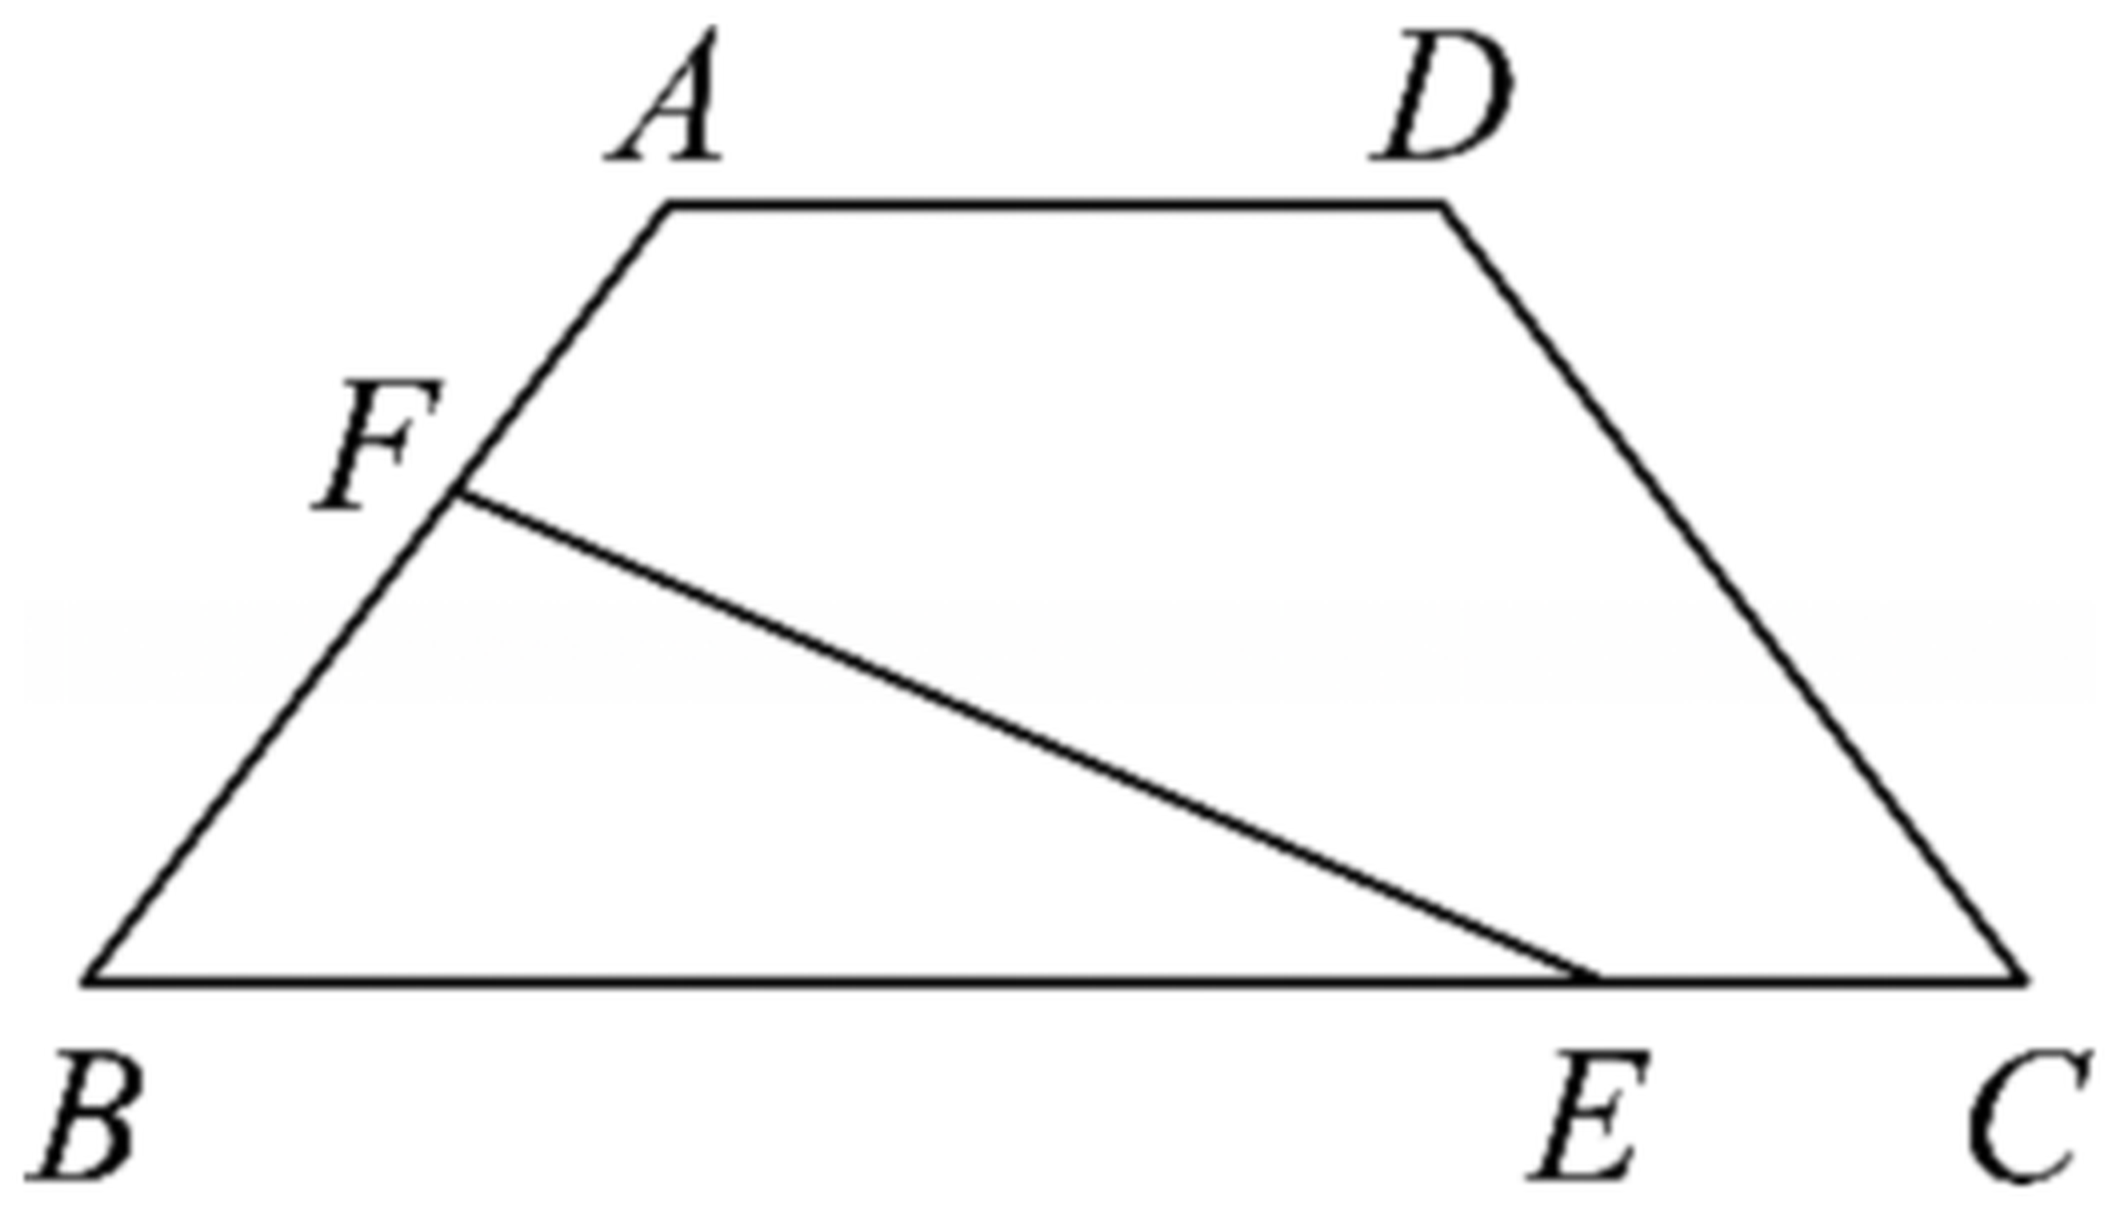
\includegraphics[width=0.46\textwidth]{figures/trapezoid_EF.png}
\end{center}

\begin{enumerate}[label=(\arabic*)]
\item 若 $EF$ 平分等腰梯形 $ABCD$ 的周长，设 $BE$ 长为 $x$，试用含 $x$ 的代数式表示
$\triangle BEF$ 的面积；
\item 是否存在线段 $EF$ 将等腰梯形 $ABCD$ 的周长和面积同时平分？若存在，求出此时 $BE$
的长；若不存在，请说明理由；
\item 是否存在线段 $EF$ 将等腰梯形 $ABCD$ 的周长和面积同时分成 $1:2$ 的两部分？
若存在，求此时 $BE$ 的长；若不存在，请说明理由.
\end{enumerate}

\ifanswer
\solbegin
\stepm{(1)}{过 $A$ 作 $AK\perp BC$ 交 $BC$ 于点 $K$，过 $F$ 作 $FG\perp BC$ 交 $BC$ 于点
$G$，}

\begin{center}
% 图取原卷截图、4× LANCZOS 放大（同梯形，多出虚线 $FG\perp BC$ 与 $AK\perp BC$
% 及两处直角符号；图只在【解析】里出现，故放进 \ifanswer 块）。
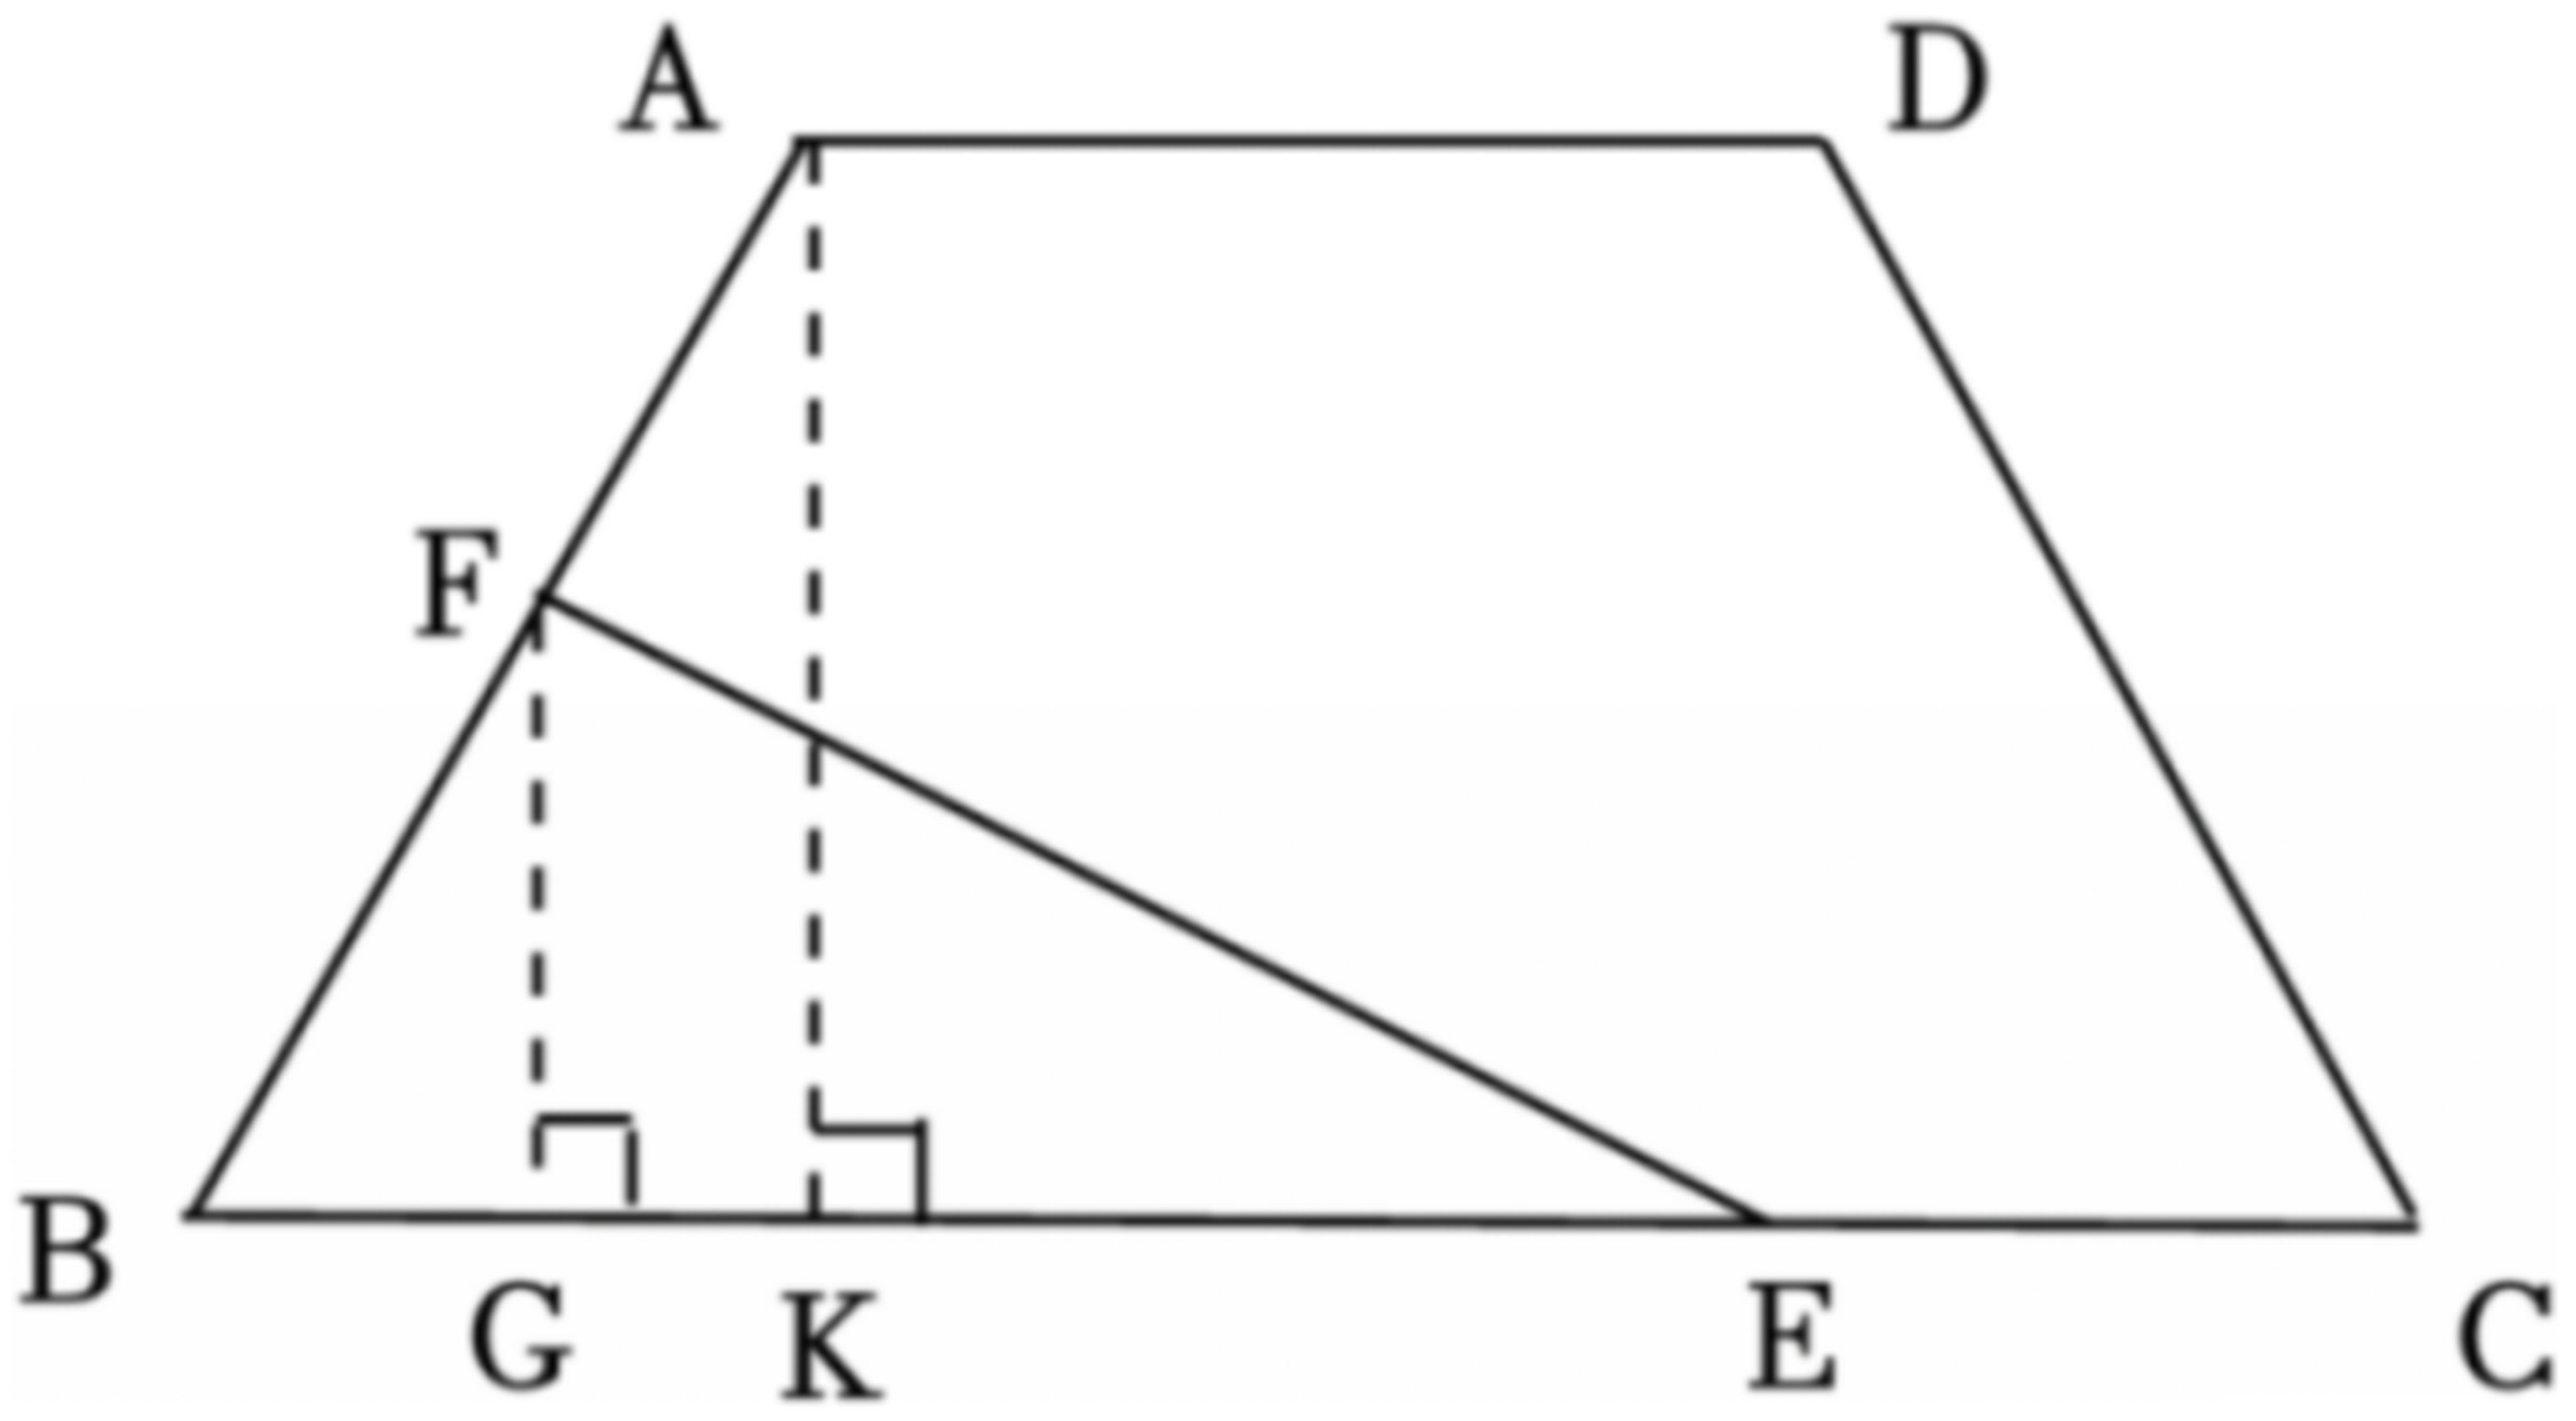
\includegraphics[width=0.62\textwidth]{figures/trapezoid_EF_aux.png}
\end{center}

\step{所以 $BK=\dfrac12\times(BC-AD)=\dfrac12\times(10-4)=3$，}
\step{$AK=\sqrt{AB^2-BK^2}=\sqrt{5^2-3^2}=4$，}
\step{由题意得，梯形 $ABCD$ 周长为 $24$，高为 $4$，面积为 $28$，}
\step{因为 $EF$ 平分等腰梯形 $ABCD$ 的周长，设 $BE$ 长为 $x$，则 $BF=12-x$，}
\step{由 $\begin{cases}0\leqslant12-x\leqslant5\\ 0\leqslant x\leqslant10\end{cases}$，
解得 $7\leqslant x\leqslant10$，}
\step{由题意得 $\triangle BFG\backsim\triangle BAK$，所以 $\dfrac{FG}{AK}=\dfrac{BF}{BA}$，
即 $\dfrac{FG}4=\dfrac{12-x}5$，}
\step{解得 $FG=\dfrac45(12-x)$，}
\step{所以 $S_{\triangle BEF}=\dfrac12BE\cdot FG
=-\dfrac25x^2+\dfrac{24}5x$（$7\leqslant x\leqslant10$）；}
\stepm{(2)}{存在，由 (1) 得 $-\dfrac25x^2+\dfrac{24}5x=\dfrac{28}2$，$x\in[7,10]$，}
\step{即 $x^2-12x+35=0$，解得 $x=7$ 或 $x=5$（舍去），}
\step{所以存在线段 $EF$ 将等腰梯形 $ABCD$ 的周长和面积同时平分，此时 $BE=7$；}
\stepm{(3)}{不存在，}
\step{情况一：$\triangle BEF$ 的面积$:$多边形 $AFECD$ 的面积 $=1:2$，
$(BE+BF):(AF+AD+DC+CE)=1:2$，}
\step{梯形周长的 $\dfrac13$ 是 $\dfrac{24}3=8$，面积的 $\dfrac13$ 是 $\dfrac{28}3$，}
\step{又因为 $BE=x$，所以 $BF=8-x$，}
\step{又因为 $\dfrac{FG}{AK}=\dfrac{BF}{BA}$，即 $\dfrac{FG}4=\dfrac{8-x}5$，
所以 $FG=\dfrac{32-4x}5$，}
\step{所以 $S_{\triangle BEF}=\dfrac12BE\times FG=-\dfrac25x^2+\dfrac{16}5x$，
所以 $\dfrac{28}3=-\dfrac25x^2+\dfrac{16}5x$，}
\step{整理得 $-3x^2+24x-70=0$，此时 $\Delta<0$，无解，故不存在；}
\step{情况二：$\triangle BEF$ 的面积$:$多边形 $AFECD$ 的面积 $=2:1$，
$(BE+BF):(AF+AD+DC+CE)=2:1$，}
\step{梯形周长的 $\dfrac13$ 为 $\dfrac{24}3=8$，面积的 $\dfrac13$ 为 $\dfrac{28}3$，
又 $BE=x$，所以 $BF=16-x$，}
\step{又 $\dfrac{FG}{AK}=\dfrac{BF}{BA}$，即 $\dfrac{FG}4=\dfrac{16-x}5$，
所以 $FG=\dfrac{64-4x}5$，}
\step{所以 $S_{\triangle BEF}=\dfrac12BE\times FG=-\dfrac25x^2+\dfrac{32}5x$，}
\step{所以 $\dfrac{28}3\times2=-\dfrac25x^2+\dfrac{32}5x$，
整理得 $-3x^2+48x-140=0$，}
\step{解得 $x=\dfrac{48+\sqrt{624}}6>10$，$x=\dfrac{48-\sqrt{624}}6<7$，
不符合题意，舍去，故不存在；}
\step{综上所述，不存在线段 $EF$ 将等腰梯形 $ABCD$ 的周长和面积同时分成 $1:2$ 的两部分.}
\solend

\fi

\ansspace[8]

\item 对集合 $\{1,2,\cdots,n\}$ 及其每一个非空子集 $A$，定义一个唯一确定的“交替和”
如下：将 $A$ 中的元素按照递减的次序排列，然后将第一个元素交替地减或加后继的元素所得的
结果，例如，子集 $\{1,2,4,6,9\}$ 的“交替和”是 $9-6+4-2+1=6$，子集 $\{5,6\}$ 的
“交替和”是 $6-5=1$，子集 $\{2\}$ 的交替和是 $2$；定义一个唯一确定的“交替积”如下：
将 $A$ 中的元素按照递减的次序排列，然后将第一个元素交替地除以或乘以后继的数所得的结果，
例如，集合 $\{1,2,4,6,9\}$ 的“交替积”是 $9\div6\times4\div2\times1=3$，
$\{5,6\}$ 的“交替积”是 $6\div5=1.2$，$\{2\}$ 的“交替积”是 $2$.

\begin{enumerate}[label=(\arabic*)]
\item 对于 $\{1,2,3,4,5,6,7,8,9\}$，求其所有子集的“交替和”的总和；
\item 对于 $\{1,2,\cdots,n\}$，求其所有子集的“交替和”的总和；
\item 对于 $\left\{n\mid\dfrac{495}{n+2}\in\N,n\in\Z\right\}$ 求其所有子集的
“交替积”的总和.
\end{enumerate}

\ifanswer
\solbegin
\stepm{(1)}{集合 $\{1,2,3,4,5,6,7,8,9\}$ 的子集中，除去 $\{9\}$ 外还有 $2^9-2$ 个
非空子集，}
\step{把这 $2^9-2$ 个非空子集两两组合后分别计算每一组中“交替和”之和，}
\step{组合原则是设 $A_i=\{9,a_1,a_2,\cdots\}$，$A_i^1=\{a_1,a_2,\cdots\}$，}
\step{集合 $A_i^1$ 的元素为集合 $A_i$ 中去掉 $9$ 的所有元素，把 $A_i$ 和 $A_i^1$
结合为一组，}
\step{显然，每组的“交替和”的和为 $9$，共有 $\dfrac{2^9-2}2$ 组，}
\step{所以，所有“交替和”之和应该为 $\dfrac{9(2^9-2)}2+9=2304$；}
\stepm{(2)}{集合 $\{1,2,\cdots,n\}$ 的子集中，除去 $\{n\}$ 外还有 $2^n-2$ 个非空子集，}
\step{把这 $2^n-2$ 个非空子集两两组合后分别计算每一组中“交替和”之和，}
\step{组合原则是设 $A_i=\{n,a_1,a_2,\cdots\}$，$A_i^1=\{a_1,a_2,\cdots\}$，}
\step{集合 $A_i^1$ 的元素为集合 $A_i$ 中去掉 $n$ 的所有元素，把 $A_i$ 和 $A_i^1$
结合为一组，}
\step{显然，每组的“交替和”的和为 $n$，共有 $\dfrac{2^n-2}2$ 组，}
% 注：下一行分子原卷印作花括号（其余同类处皆用圆括号），照抄未改，见文件头“原卷存疑”③。
\step{所以，所有“交替和”之和应该为 $\dfrac{n\{2^n-2\}}2+n=n\cdot2^{n-1}$；}
\stepm{(3)}{集合 $\left\{n\mid\dfrac{495}{n+2}\in\N,n\in\Z\right\}
=\{493,163,97,53,43,31,13,9,7,3,1,-1\}$，}
\step{其中除去 $\{-1\}$ 外还有 $2^{12}-2$ 个非空子集，}
% 注：下一行原卷把“把这”重复印了一次（“把这把这”），照抄未改，见文件头“原卷存疑”②。
\step{把这把这 $2^{12}-2$ 个非空子集两两组合后分别计算每一组中“交替积”之和，}
\step{组合原则是设 $A_j=\{-1,a_1,a_2,\cdots\}$，$A_j^1=\{a_1,a_2,\cdots\}$，}
\step{集合 $A_j^1$ 的元素为集合 $A_j$ 中去掉 $-1$ 的所有元素，把 $A_j$ 和 $A_j^1$
结合为一组，}
\step{显然，每组的“交替积”的和为 $0$，共有 $\dfrac{2^{12}-2}2$ 组，}
\step{所以，所有“交替积”之和应该为 $\dfrac{2^{12}-2}2\times0-1=-1$.}
\solend

\fi

\ansspace*[10]

\end{enumerate}

\end{document}
"
% 紧凑版：xelatex "\def\iscompact{1}% 高一30_南洋模范中学_开学考.tex
%   —— 高一上数学“2026-2027 年南洋模范中学高一上开学考”（试卷版/答案版）
% 试卷版：xelatex 高一30_南洋模范中学_开学考.tex
% 答案版：xelatex "\def\isanswer{1}% 高一30_南洋模范中学_开学考.tex
%   —— 高一上数学“2026-2027 年南洋模范中学高一上开学考”（试卷版/答案版）
% 试卷版：xelatex 高一30_南洋模范中学_开学考.tex
% 答案版：xelatex "\def\isanswer{1}% 高一30_南洋模范中学_开学考.tex
%   —— 高一上数学“2026-2027 年南洋模范中学高一上开学考”（试卷版/答案版）
% 试卷版：xelatex 高一30_南洋模范中学_开学考.tex
% 答案版：xelatex "\def\isanswer{1}\input{高一30_南洋模范中学_开学考.tex}"
% 紧凑版：xelatex "\def\iscompact{1}\input{高一30_南洋模范中学_开学考.tex}"
%
% 原始材料是微信公众号图文（公众号“魔都数学加油站”连载“27学年高一 30”，2026-09-23 发布，
% 原文标题“27学年高一30——2026-2027年上海市南洋模范中学高一上开学考”），
% 正文为 11 张 PNG 页。**同一篇里各页分辨率不一致**——第 2、3、9、10 页 4762×6735，
% 其余七页 2560×3620（已逐页打开确认，非下载缺档），取的是 mmbiz.qpic.cn/<hash>/0 的原图档。
% 原文本身就是一份**讲评版**：填空第 3—7 题下方印【答案】，第 8—12 题与其后各题印【解析】。
% 试题文字、答案与解析均照原卷录入，未改内容。卷面的粉色斜水印属水印，未录入。
%
% 卷首标题：原卷印作“2026-2027 年南洋模范中学高一上开学考”（公众号标题里的“上海市”
% 三字卷面标题行没有，本稿照卷面），年份区间按全稿惯例排 en dash，前缀照原卷保留“年”。
%
% 与原卷的排版差异（均已在 README“说明”中交代）：
%   ① 原文自**第 3 题**起（第 1、2 题未在该文中发布），故本稿题号亦自 3 起；
%   ② 原卷本就印有“一、填空题”“二、选择题”“三、解答题”三节标题，本稿照原卷分节，
%      只把标题改排成全稿统一的“大节标题”样式；
%   ③ 原卷填空第 3—7 题只印【答案】行、第 8 题起印【解析】（选择题答案写在解析末句
%      “故选 D／B”里），本稿统一改为试卷版隐去、答案版以 \ans{}／\ifanswer 块给出，
%      两版彻底分离；
%   ④ 子集符号原卷两种并用：第 7 题题干两处、第 19(2) 题作带下划线的 $\subseteq$，
%      第 17(2) 题解析作真包含的 $\subset$，本稿分别照录为 $\sub$ 与 $\subset$；
%   ⑤ 补集符号原卷一律作**上横线**（$\overline{A}$、$\overline{B}$），本稿照录；
%   ⑥ 原卷的实数集 R 一律作斜体（第 4 题、第 17 题与第 19 题题干的 $U=R$），
%      第 21(3) 题的自然数集与整数集作**粗体** $\mathbf{N}$、$\mathbf{Z}$，
%      本稿按全稿惯例统一写作 $\R$、$\N$、$\Z$；
%   ⑦ 原卷填空的横线约两个字宽，本稿按全稿惯例统一排 \blankline[4.4em]；
%   ⑧ 原卷未印副标题，本稿按全稿惯例补出副标题“集合与常用逻辑用语”——但本卷是开学考，
%      范围不止这一章：第 18 题是速度—时间图象题、第 20 题是等腰梯形的周长/面积平分问题，
%      副标题只标了主章节（见文末“高一30 专记”）；
%   ⑨ 第 13、14、18、20 题的图印在题干右侧、第 16 题的三幅图印在【解析】里的下一页顶部、
%      第 20 题【解析】另有一张带辅助线的图，本稿一律移至题干或解析之后；
%      图取原卷截图、4× LANCZOS 放大（见各 \includegraphics 前的注释）。
%
% 原卷存疑三处（均照抄原卷、未改，见源码中该处上方注释）：
%   ① 第 10 题【解析】验证“破晓集”时写的是 $\notin A$、$\in A$（如“$-2-2=-4\notin A$”），
%      但该处讨论的集合原题设里叫 $P$，同题②的“$x+y=2(k_1+k_2)\in A$”亦然——
%      本稿照抄未改（按文意应为 $P$）；
%   ② 第 21 题【解析】(3) 有“把这把这 $2^{12}-2$ 个非空子集”（“把这”重复印了一次）；
%   ③ 同题 (2) 的结论式分子原卷印作花括号 $\dfrac{n\{2^n-2\}}{2}$（其余同类处皆用圆括号）。

\documentclass[a4paper,11pt]{article}
\usepackage{common}

\begin{document}

\examtitlest[3]{2026--2027 年南洋模范中学高一上开学考}{集合与常用逻辑用语}

\bigsec{一、填空题}

\begin{enumerate}
\setcounter{enumi}{2}

\item 若集合 $A=\{x\mid x^2-2kx+7k=0\}$ 有且仅有三个真子集，则 $k$ 的取值范围是
\blankline[4.4em].

\ans{$(-\infty,0)\cup(7,+\infty)$}

\item “存在 $x\in\R$，使得 $x^2+2x+5=0$”的否定形式是 \blankline[4.4em].

\ans{对任何 $x\in\R$，都有 $x^2+2x+5\neq0$}

\item 下列命题中，$p$ 是 $q$ 的必要非充分条件的是 \blankline[4.4em].

① $p:x>2$ 且 $y>3$，$q:x+y>5$；

② $p$：四边形的四个角都相等，$q$：四边形是正方形.

\ans{②}

\item 若“条件 $\alpha:2\leqslant x\leqslant4$”是“条件 $\beta:3m-1\leqslant x\leqslant-m$”的
充分非必要条件，则 $m$ 的取值范围是 \blankline[4.4em].

\ans{$(-\infty,-4]$}

\item 满足 $\{1\}\sub M\sub\{1,2,4,5\}$ 的集合 $M$ 的个数为 \blankline[4.4em] 个.

\ans{$8$}

\item 已知集合 $A=\{1,2\}$，集合 $B=\{x\mid ax=6\}$，若 $A\cup B=A$，则 $a$ 的所有取值
构成的集合为 \blankline[4.4em].

\ifanswer
\solbegin
\step{因为 $A\cup B=A$，所以 $B\sub A$，}
\step{当 $a=0$ 时，$B=\varnothing$，满足 $B\sub A$；}
\step{当 $a\neq0$ 时，$B=\left\{\dfrac6a\right\}$，则 $\dfrac6a=1$ 或 $\dfrac6a=2$，
解得 $a=6$ 或 $a=3$，}
\step{综上所述，$a$ 的所有取值构成的集合为 $\{0,3,6\}$.}
\solend

\fi

\item 对于集合 $M$、$N$，定义 $M-N=\{x\mid x\in M\text{ 且 }x\notin N\}$，
$M\oplus N=(M-N)\cup(N-M)$，设 $A=\{y\mid y=|x|,x\in\R\}$，
$B=\{y\mid y=-(x-1)^2+2,x\in\R\}$，则 $A\oplus B=$ \blankline[4.4em].

\ifanswer
\solbegin
\step{由已知 $A=[0,+\infty)$，$B=(-\infty,2]$，}
\step{由于 $A-B=(2,+\infty)$，$B-A=(-\infty,0)$，}
\step{故 $A\oplus B=(A-B)\cup(B-A)=(-\infty,0)\cup(2,+\infty)$.}
\solend

\fi

\item 设 $P$ 为非空实数集满足：对任意给定的 $x$、$y\in P$（$x$、$y$ 可以相同），都有
$x+y\in P$，$x-y\in P$，$xy\in P$，则称 $P$ 为破晓集. 关于破晓集有下列结论：
①集合 $P=\{-2,-1,0,1,2\}$ 为破晓集；②集合 $P=\{x\mid x=2n,n\in\Z\}$ 为破晓集；
③若集合 $P_1$、$P_2$ 为破晓集，则 $P_1\cup P_2$ 为破晓集；④若集合 $P$ 为破晓集，
则一定有 $0\in P$；⑤若集合 $P_1$、$P_2$ 为破晓集，则 $P_1\cap P_2$ 为破晓集；
其中正确结论的序号是 \blankline[4.4em].

\ifanswer
\solbegin
% 注：以下几步原卷把该集合记作 $A$（题设里叫 $P$），照抄未改，见文件头“原卷存疑”①。
\step{对于①：$-2-2=-4\notin A$，故集合 $P=\{-2,-1,0,1,2\}$ 不为破晓集，故①错误；}
\step{②设 $x$、$y\in A$，则 $x=2k_1$，$y=2k_2$，且 $k_1$、$k_2\in\Z$，}
\step{故 $x+y=2(k_1+k_2)\in A$，$x-y=2(k_1-k_2)\in A$，$xy=4k_1k_2\in A$，}
\step{故集合 $P=\{x\mid x=2n,n\in\Z\}$ 为破晓集，故②正确；}
\step{③若集合 $P_1$、$P_2$ 为破晓集，设 $P_1=\{x\mid x=2k,k\in\Z\}$，
$P_2=\{x\mid x=3k,k\in\Z\}$，}
\step{但是 $P_1\cup P_2$ 不为破晓集，如 $x=2$，$y=3$ 时，$x+y=5$，
故 $5\notin(P_1\cup P_2)$，故③错误；}
\step{④若集合 $P$ 为破晓集，则取 $x=y$，$x-y=0\in A$，则一定有 $0\in P$，故④正确.}
\step{⑤正确；}
\step{故正确的是②④⑤.}
\solend

\fi

\item 已知集合 $M$ 的元素均为正整数，定义集合 $M$ 的“变项和”为：将 $M$ 中每个元素 $m$
都乘以 $(-1)^m$ 后再求和. 若集合 $A=\{n\mid1\leqslant n\leqslant10,n\in\N\}$，则集合 $A$
的所有非空子集的“变项和”的总和为 \blankline[4.4em].

\ifanswer
\solbegin
\step{$A$ 集合的所有非空子集中，每个元素出现的次数都是
$(2^{10}-1)-(2^9-1)=2^9$，}
\step{则集合 $A$ 的所有非空子集的“变项和”的总和为
$1\times(-1)^1\times2^9+2\times(-1)^2\times2^9+\cdots+10\times(-1)^{10}\times2^9$}
\step{$=(-1+2-3+4-\cdots-9+10)\times2^9=5\times2^9=2560$.}
\solend

\fi

\item 已知集合 $A=[t,t+1]\cup[t+4,t+9]$，$0\notin A$，存在正数 $\lambda$，使得对任意
$a\in A$，都有 $\dfrac\lambda a\in A$，则 $t$ 的值是 \blankline[4.4em].

\ifanswer
\solbegin
\step{当 $t>0$ 时，当 $a\in[t,t+1]$ 时，$\dfrac\lambda a\in[t+4,t+9]$，}
\step{当 $a\in[t+4,t+9]$ 时，$\dfrac\lambda a\in[t,t+1]$，}
\step{即当 $a=t$ 时，$\dfrac\lambda a\leqslant t+9$；当 $a=t+9$ 时，
$\dfrac\lambda a\geqslant t$，即 $\lambda=t(t+9)$；}
\step{当 $a=t+1$ 时，$\dfrac\lambda a\geqslant t+4$，当 $a=t+4$ 时，
$\dfrac\lambda a\leqslant t+1$，即 $\lambda=(t+1)(t+4)$，}
\step{所以 $t(t+9)=(t+1)(t+4)$，解得 $t=1$.}
\step{当 $t+1<0<t+4$ 时，当 $a\in[t,t+1]$ 时，$\dfrac\lambda a\in[t,t+1]$.}
\step{当 $a\in[t+4,t+9]$ 时，则 $\dfrac\lambda a\in[t+4,t+9]$，}
\step{即当 $a=t$ 时，$\dfrac\lambda a\leqslant t+1$，当 $a=t+1$ 时，
$\dfrac\lambda a\geqslant t$，即 $\lambda=t(t+1)$，}
\step{即当 $a=t+4$ 时，$\dfrac\lambda a\leqslant t+9$，当 $a=t+9$ 时，
$\dfrac\lambda a\geqslant t+4$，即 $\lambda=(t+4)(t+9)$，}
\step{所以 $t(t+1)=(t+4)(t+9)$，解得 $t=-3$.}
\step{当 $t+9<0$ 时，同理可得无解.}
\step{综上，$t$ 的值为 $1$ 或 $-3$.}
\solend

\fi

\end{enumerate}

\bigsec{二、选择题}

\begin{enumerate}
\setcounter{enumi}{12}

% 这道题是“题干 + 图 + 选项”约 6cm 的一整块，页末放不下就会被拆开（切页审计的 A 类），
% 故在题前先量一次页高：不够就把整道题干连图带选项一起挪到次页。
\needvspace{6.5cm}
\item 设 $U=\{1,2,3,4,5\}$，$A$、$B$ 都是 $U$ 的子集，且 $A\cap B=\{5\}$，
$\overline{A}\cap B=\{4\}$，$\overline{A}\cap\overline{B}=\{1,2\}$，
则以下四个判断中正确的是\mbox{（\quad）}

\begin{center}
% 图取原卷截图、4× LANCZOS 放大（原卷把图印在题干右侧，本稿移至此处，见文件头⑨）。
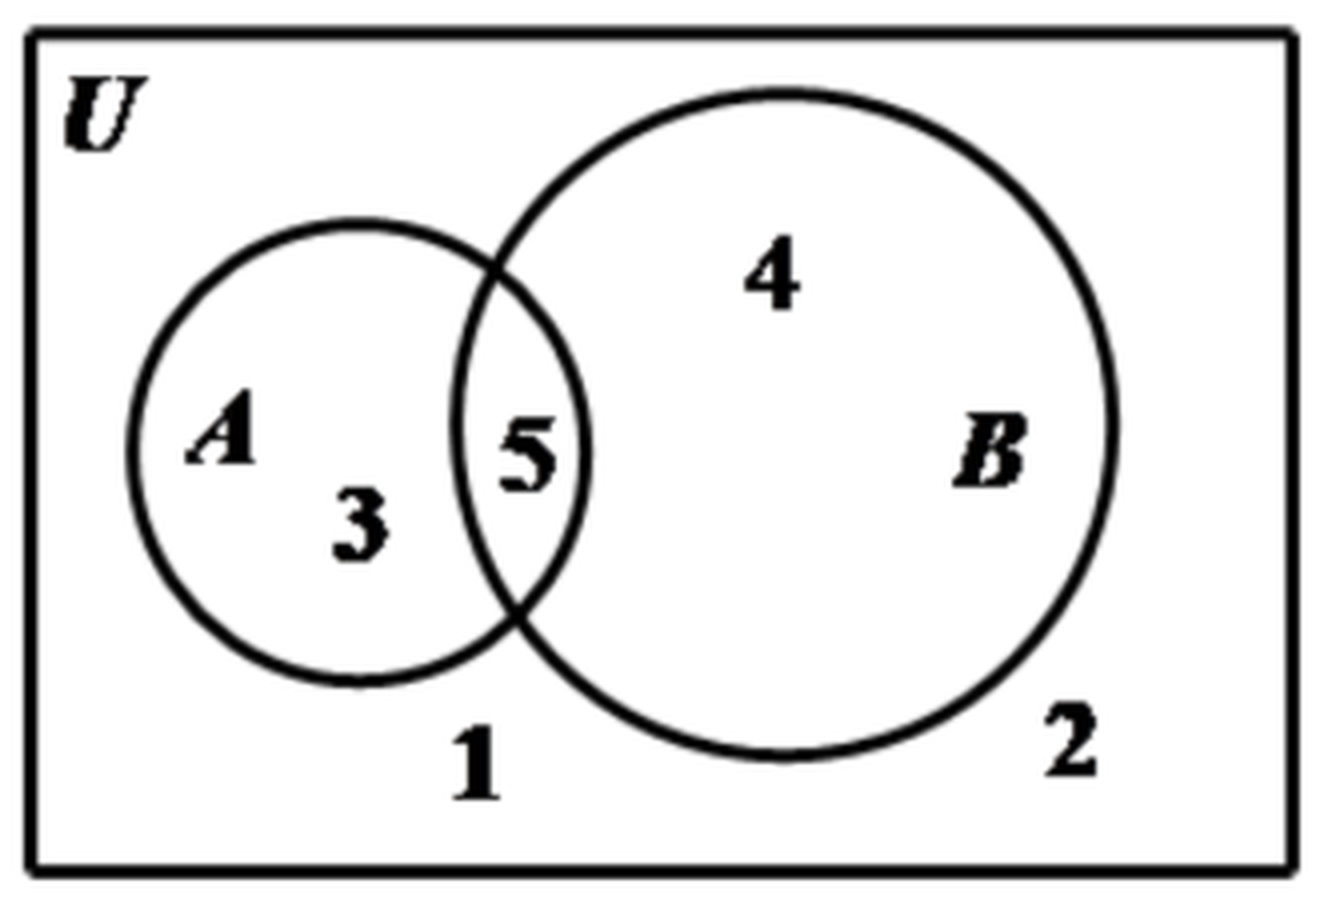
\includegraphics[width=0.28\textwidth]{figures/venn_U5_AB.png}
\end{center}

\keepwithprev
A. $3\notin A$ 且 $3\notin B$\qquad\qquad B. $3\in A$ 且 $3\in B$

C. $3\notin A$ 且 $3\in B$\qquad\qquad D. $3\in A$ 且 $3\notin B$

\ans{$D$}

\ifanswer
\solbegin
\step{画出韦恩图，得 $A=\{5,3\}$，$B=\{5,4\}$，}
\step{则 $3\in A$ 且 $3\notin B$. 故选 $D$.}
\solend

\fi

% 同第 13 题：整块（题干 + 图 + 选项）在答案版还要再挂【答案】【解析】，页末更易被拆开。
\needvspace{7.5cm}
\item 如图表示图形阴影部分的是\mbox{（\quad）}

\begin{center}
% 图取原卷截图、4× LANCZOS 放大（三圆 $A$、$B$、$C$，阴影为整个 $A$ 圆加 $B\cap C$）。
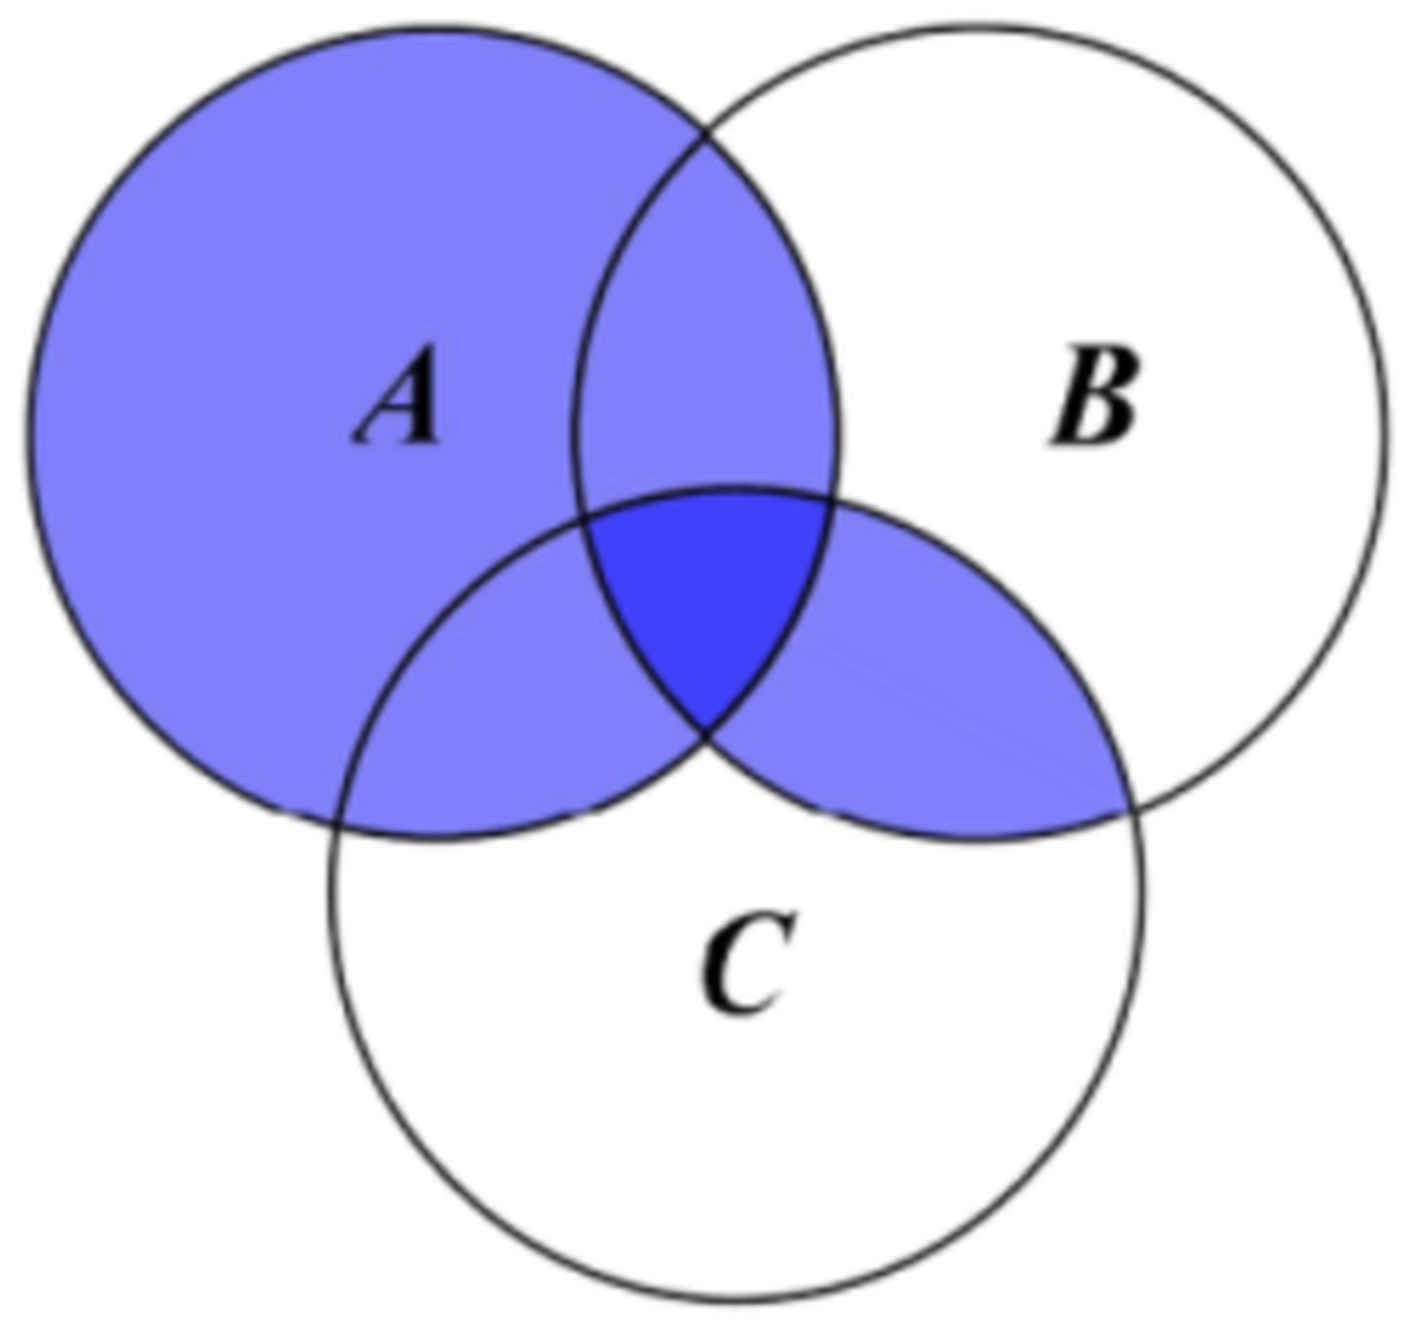
\includegraphics[width=0.30\textwidth]{figures/venn_A_union_BC.png}
\end{center}

\keepwithprev
A. $(A\cup C)\cap(B\cup C)$\qquad\qquad B. $(A\cup B)\cap(A\cup C)$

C. $(A\cup B)\cap(B\cup C)$\qquad\qquad D. $(A\cup B)\cap C$

\ans{$B$}

\ifanswer
\solbegin
\step{图中阴影部分表示元素满足是 $A$ 中的元素，或者是 $B$ 与 $C$ 的公共元素，}
\step{故可以表示为 $A\cup(B\cap C)$，也可以表示为 $(A\cup B)\cap(A\cup C)$.
故选 $B$.}
\solend

\fi

\item 设集合 $M=\left\{x\mid m\leqslant x\leqslant m+\dfrac34\right\}$，
$N=\left\{x\mid n-\dfrac13\leqslant x\leqslant n\right\}$，且 $M$、$N$ 都是集合
$\{x\mid0\leqslant x\leqslant1\}$ 的子集，如果把 $b-a$ 叫做集合
$\{x\mid a\leqslant x\leqslant b\}$ 的“长度”，那么集合 $M\cap N$ 的“长度”的
最小值是\mbox{（\quad）}

\keepwithprev
A. $\dfrac23$\qquad B. $\dfrac1{12}$\qquad C. $\dfrac13$\qquad D. $\dfrac5{12}$

\ans{$B$}

\ifanswer
\solbegin
\step{$M$ 的长度为 $\dfrac34$，$N$ 的长度为 $\dfrac13$，}
\step{当集合 $M\cap N$ 的长度的最小值时，$M$ 与 $N$ 应分别在区间 $[0,1]$ 的左右两端，}
\step{故 $M\cap N$ 的长度的最小值是 $\dfrac34+\dfrac13-1=\dfrac1{12}$，故选 $B$.}
\solend

\fi

\item 定义集合运算 $A-B=\{x\mid x\in A\text{ 且 }x\notin B\}$ 称为集合 $A$ 与集合 $B$ 的
差集；定义集合运算 $A\Delta B=(A-B)\cup(B-A)$ 称为集合 $A$ 与集合 $B$ 的对称差，
有以下 $4$ 个等式：① $A\Delta B=B\Delta A$；② $(A\Delta B)\Delta C=A\Delta(B\Delta C)$；
③ $A\cap(B\Delta C)=(A\cap B)\Delta(A\cap C)$；
④ $A\cup(B\Delta C)=(A\cup B)\Delta(A\cup C)$，
则 $4$ 个等式中恒成立的是\mbox{（\quad）}

\keepwithprev
A. ①②\qquad B. ①②③\qquad C. ①②④\qquad D. ①②③④

\ans{$B$}

\ifanswer
\solbegin
\step{对于①，由 $B\Delta A=(B-A)\cup(A-B)=(A-B)\cup(B-A)=A\Delta B$，
所以①正确；}
\step{对于②，由 $A-B=\{x\mid x\in A\text{ 且 }x\notin B\}
=\{x\mid x\in A,x\notin(A\cap B)\}=A-(A\cap B)$，}
\step{同理可得 $B-A=B-(A\cap B)$，}
\step{则 $A\Delta B=(A-B)\cup(B-A)=(A\cup B)-(A\cap B)$，}
\step{所以 $(A\Delta B)\Delta C=(A\Delta B)\cup C-(A\Delta B)\cap C$，}
\step{所以表示的集合为图（1）中阴影部分所表示的集合，如图所示，}
\step{同理 $A\Delta(B\Delta C)=A\cup(B\Delta C)-A\cap(B\Delta C)$，
也表示图（1）中阴影部分所表示的集合，}
\step{所以 $(A\Delta B)\Delta C=A\Delta(B\Delta C)$，所以②正确；}

\begin{center}
% 图取原卷截图、4× LANCZOS 放大（原卷印在下一页顶部，共三幅三圆韦恩图：
% 图（1）一幅、图（2）左右两幅，图（2）两幅下方各有一行式子标注）。
% 图只在【解析】里出现，故放进 \ifanswer 块，试卷版不排。
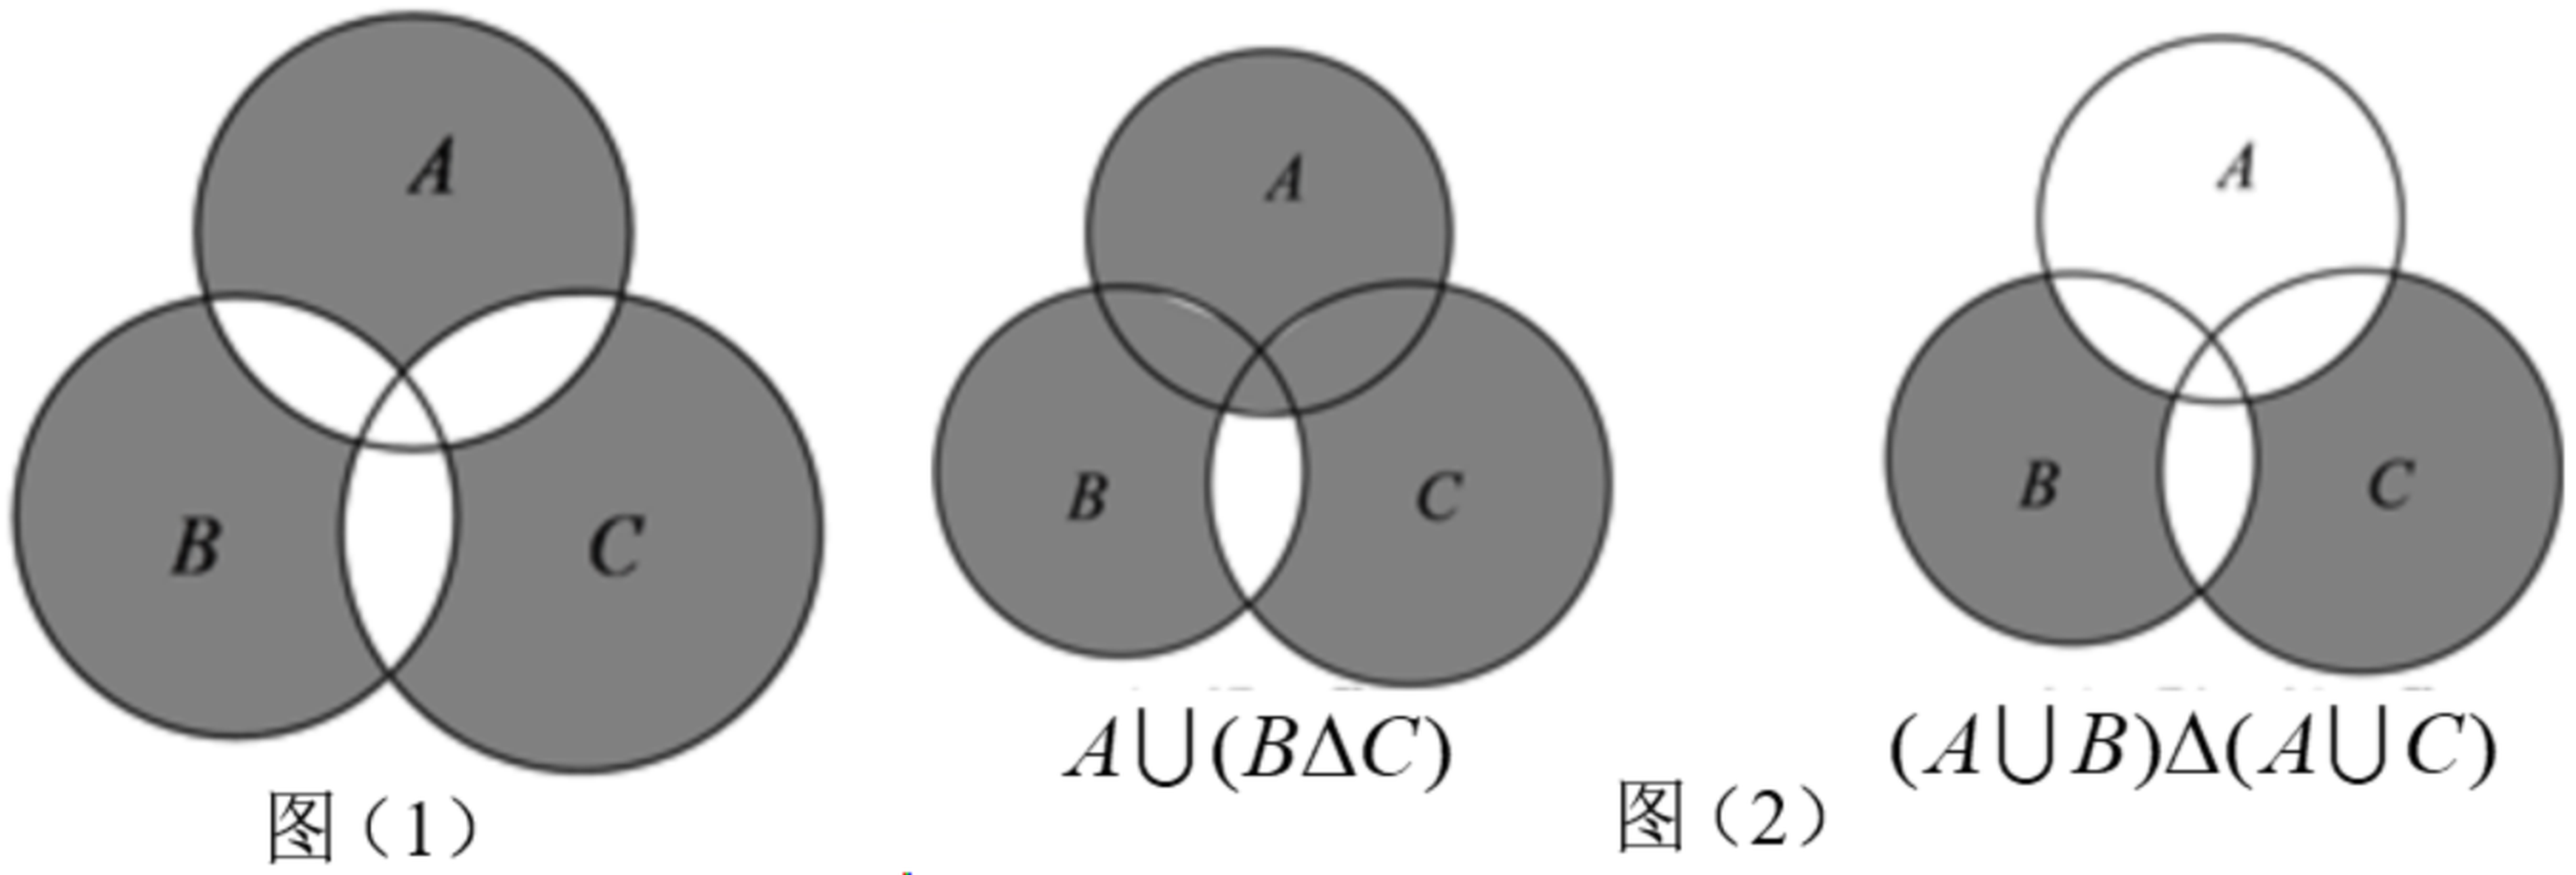
\includegraphics[width=0.86\textwidth]{figures/venn_symdiff3.png}
\end{center}

\step{对于③，由 $A\cap(B\Delta C)=A\cap(B\cup C-B\cap C)
=A\cap(B\cup C)-A\cap(B\cap C)$}
\step{$=(A\cap B)\cup(A\cap C)-(A\cap B)\cap(A\cap C)=(A\cap B)\Delta(A\cap C)$，
所以③正确；}
\step{对于④，如图（2）所示，$A\cup(B\Delta C)\neq(A\cup B)\Delta(A\cup C)$，
所以④错误.}
\step{故选 $B$.}
\solend

\fi

\end{enumerate}

\bigsec{三、解答题}

\begin{enumerate}
\setcounter{enumi}{16}

\item 已知集合 $M=\{x\mid a-1\leqslant x\leqslant2a+3\}$，$P=\{x\mid-2<x\leqslant4\}$，
全集 $U=\R$.

\begin{enumerate}[label=(\arabic*)]
\item 当 $a=2$ 时，求 $M\cap P$；
\item 若 $x\in P$ 是 $x\in M$ 的必要不充分条件，求实数 $a$ 的取值范围.
\end{enumerate}

\ifanswer
\solbegin
\stepm{(1)}{当 $a=2$ 时，集合 $M=\{x\mid1\leqslant x\leqslant7\}$，}
\step{所以 $M\cap P=\{x\mid1\leqslant x\leqslant4\}$；}
\stepm{(2)}{因为 $x\in P$ 是 $x\in M$ 的必要不充分条件，所以 $M\subset P$，}
\step{当 $M=\varnothing$ 时，$a-1>2a+3$，解得 $a<-4$，}
\step{当 $M\neq\varnothing$ 时，则
$\begin{cases}a-1\leqslant2a+3\\ a-1>-2\\ 2a+3\leqslant4\end{cases}$，
解得 $-1<a\leqslant\dfrac12$，}
\step{综上所述，实数 $a$ 的取值范围为
$(-\infty,-4)\cup\left(-1,\dfrac12\right]$.}
\solend

\fi

\ansspace[6]

\item 一辆汽车在某段路程中的行驶速度与时间的关系如图：

\begin{center}
% 图取原卷截图、4× LANCZOS 放大（速度—时间图：纵轴 $v/(\mathrm{km/h})$、
% 横轴 $t(\mathrm{h})$，$t\in[0,1]$、$[1,2]$、$[2,3]$ 三段矩形条高 50、80、90）。
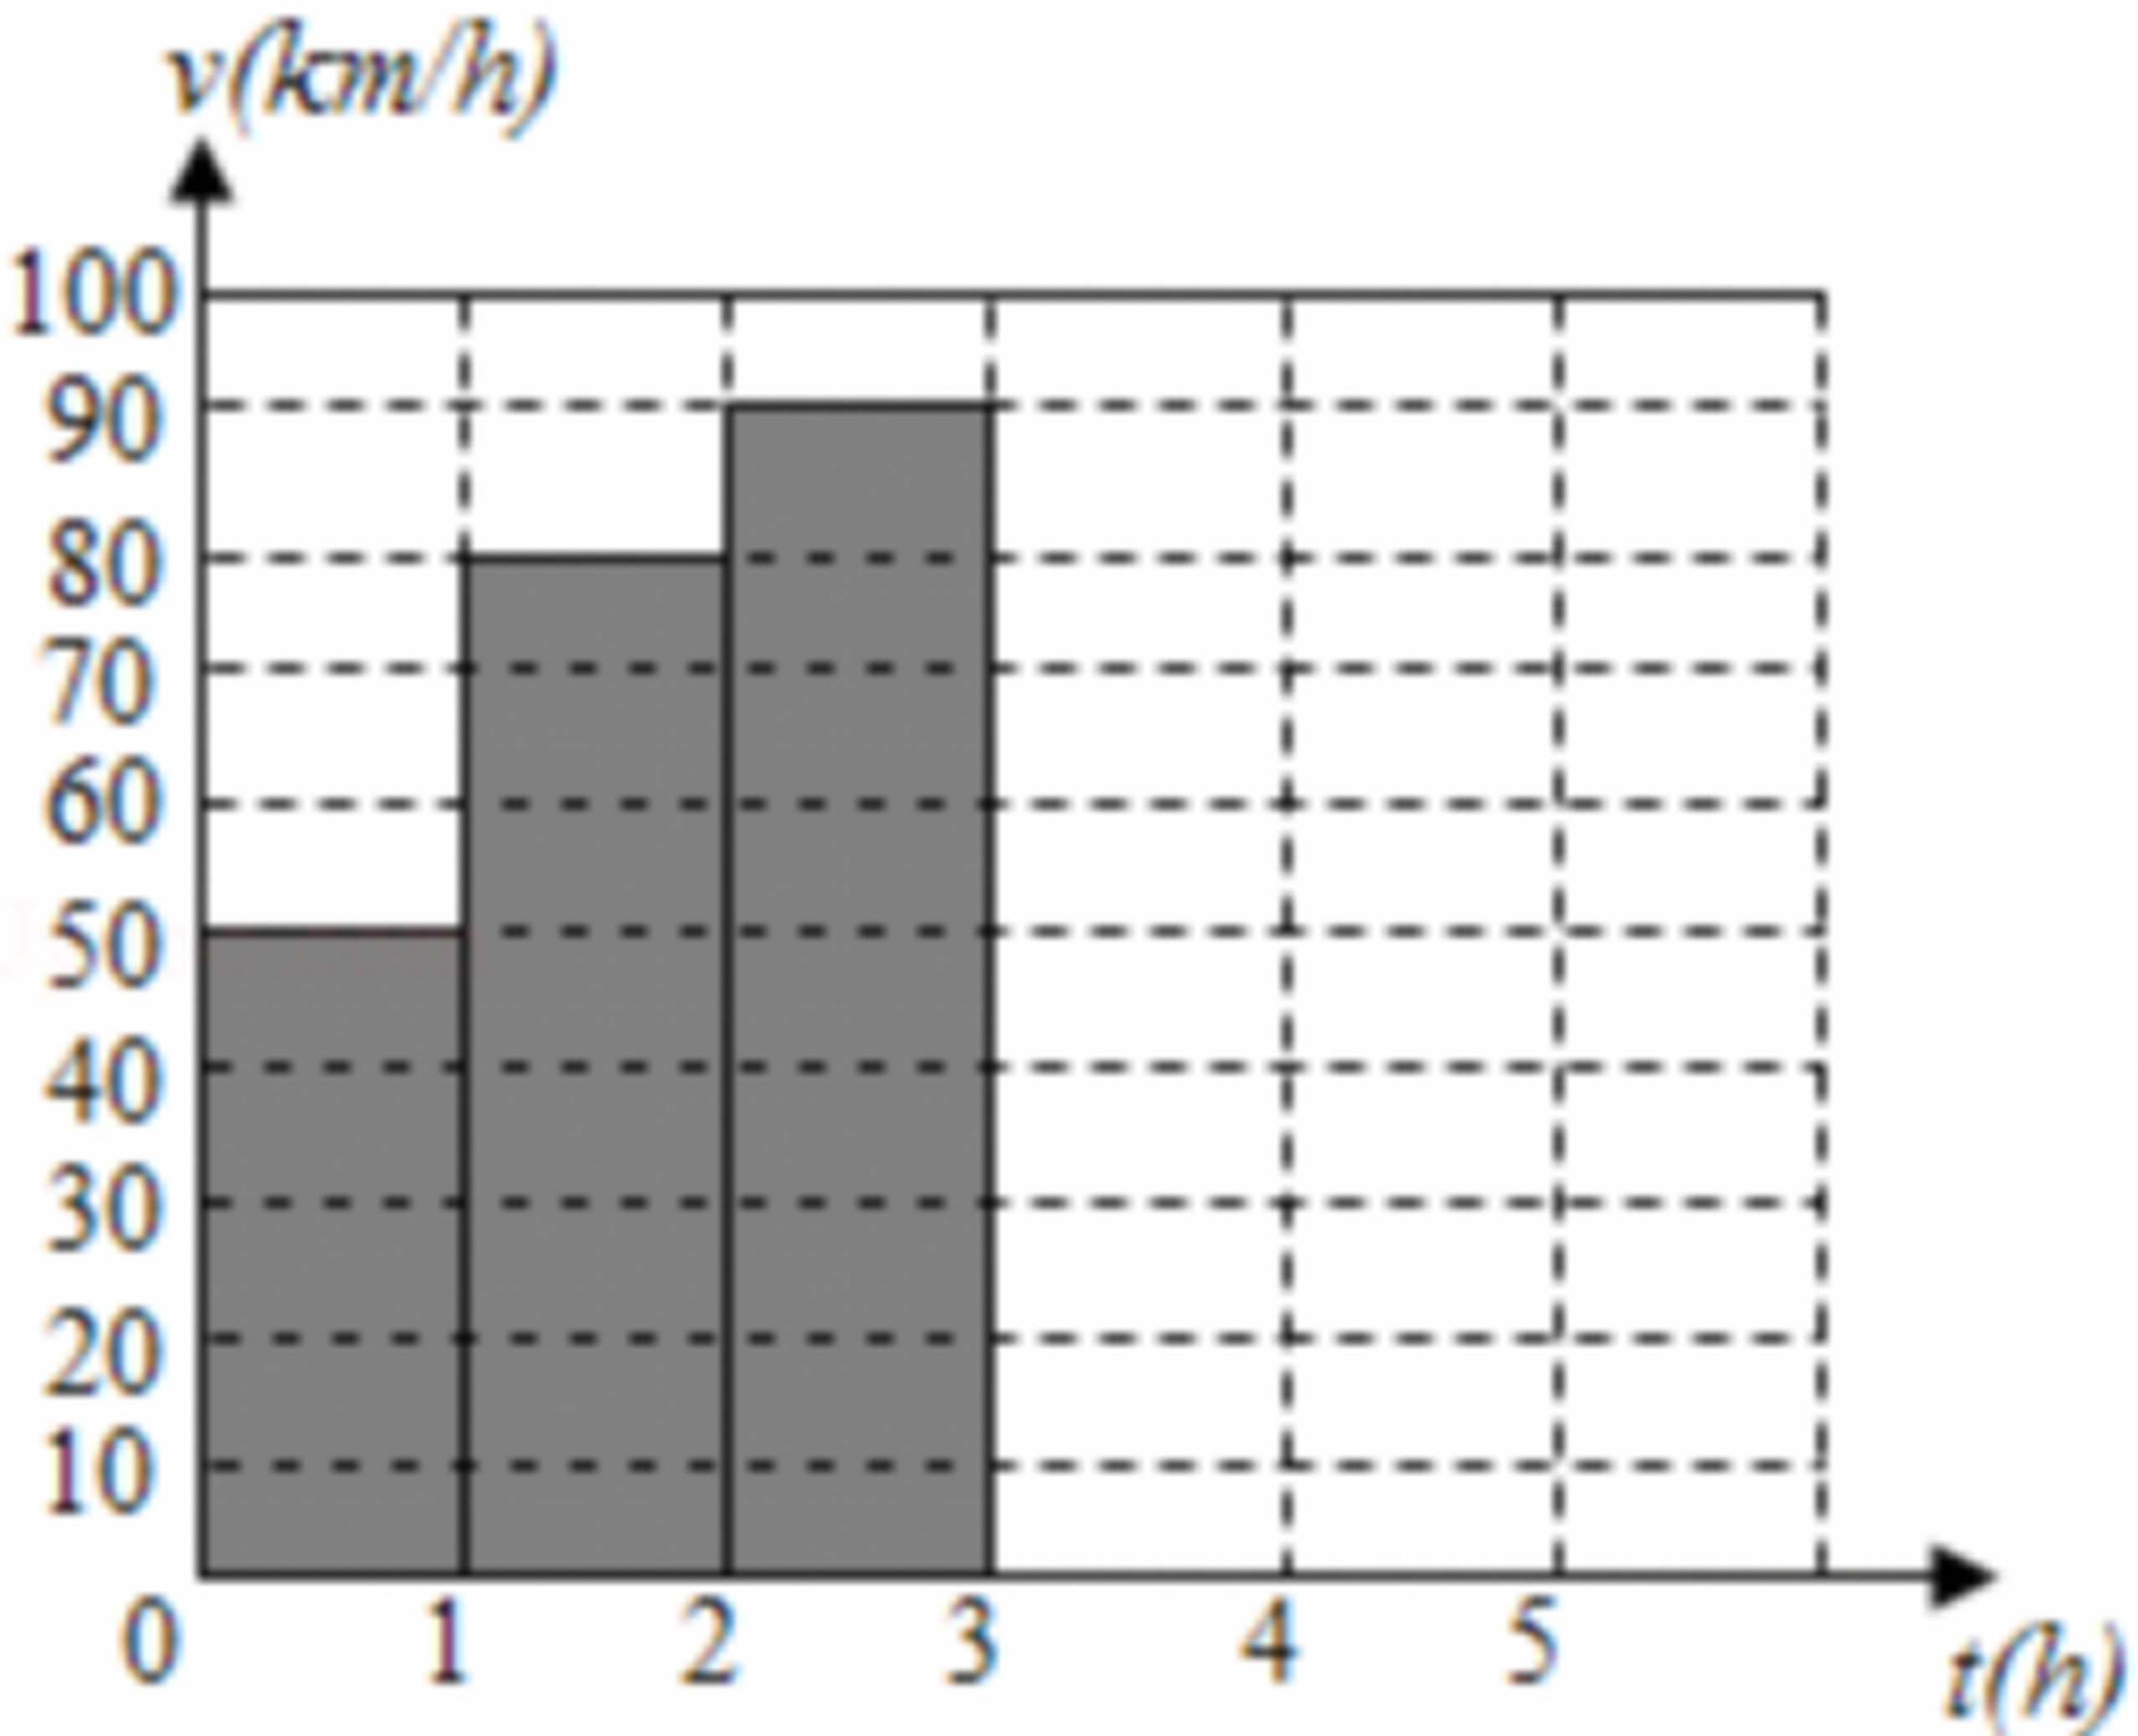
\includegraphics[width=0.52\textwidth]{figures/speed_time_bars.png}
\end{center}

\begin{enumerate}[label=(\arabic*)]
\item 求图中阴影部分的面积，并说明所求面积的实际意义；
\item 假设这辆汽车的里程表在汽车行驶这段路程前的读数为 $2004\,\mathrm{km}$，
试将汽车行驶这段路程时汽车里程表读数 $S$ 表示为时间 $t$ 的函数，
并求出当汽车里程表读数为 $2094\,\mathrm{km}$ 时，汽车行驶了多少时间？
\end{enumerate}

\ifanswer
\solbegin
\stepm{(1)}{由一辆汽车在某段路程中的行驶速度与时间的关系图，}
\step{得阴影部分的面积为 $50\times1+80\times1+90\times1=220$，}
\step{阴影部分的面积表示汽车在 $3$ 小时内行驶的路程为 $220\,\mathrm{km}$.}
\stepm{(2)}{$S=\begin{cases}
50t+2004,&0\leqslant t<1\\
80(t-1)+2054,&1\leqslant t<2\\
90(t-2)+2134,&2\leqslant t\leqslant3
\end{cases}$}
\step{令 $80(t-1)+2054=2094$，解得 $t=1.5$，所以汽车行驶 $1.5$ 小时.}
\solend

\fi

\ansspace[6]

\item 已知集合 $A=\{x\mid x<-2\text{ 或 }x\geqslant3\}$，$U=\R$.

\begin{enumerate}[label=(\arabic*)]
\item 求 $\overline{A}$；
\item 若 $B=\{x\mid mx-1>0\}$，当 $B\sub A$ 时，求实数 $m$ 的取值范围；
\item 若 $B=\{x\mid2m-6\leqslant x\leqslant m+4\}$，当 $B\cap\overline{A}=\varnothing$ 时，
求实数 $m$ 的取值范围.
\end{enumerate}

\ifanswer
\solbegin
\stepm{(1)}{因为集合 $A=\{x\mid x<-2\text{ 或 }x\geqslant3\}$，$U=\R$，
所以 $\overline{A}=\{x\mid-2\leqslant x<3\}$；}
\stepm{(2)}{当 $m=0$ 时，$B=\varnothing$，符合题意，}
\step{当 $m>0$ 时，$B=\left\{x\mid x>\dfrac1m\right\}$，则 $\dfrac1m\geqslant3$，
解得 $0<m\leqslant\dfrac13$，}
\step{当 $m<0$ 时，$B=\left\{x\mid x<\dfrac1m\right\}$，则 $\dfrac1m\leqslant-2$，
解得 $-\dfrac12\leqslant m<0$，}
\step{综上所述，实数 $m$ 的取值范围 $\left[-\dfrac12,\dfrac13\right]$；}
\stepm{(3)}{由题意得 $B=\{x\mid2m-6\leqslant x\leqslant m+4\}$，
$\overline{A}=\{x\mid-2\leqslant x<3\}$，且 $B\cap\overline{A}=\varnothing$，}
\step{当 $B=\varnothing$ 时，$2m-6>m+4$，解得 $m>10$，}
\step{当 $B\neq\varnothing$ 时，则 $\begin{cases}2m-6\leqslant m+4\\ m+4<-2\end{cases}$
或 $\begin{cases}2m-6\leqslant m+4\\ 2m-6\geqslant3\end{cases}$，}
\step{解得 $m<-6$ 或 $\dfrac92\leqslant m\leqslant10$，}
\step{综上所述，实数 $m$ 的取值范围为
$(-\infty,-6)\cup\left[\dfrac92,+\infty\right)$.}
\solend

\fi

\ansspace[8]

\item 在等腰梯形 $ABCD$ 中，$AB=DC=5$，$AD=4$，$BC=10$. 点 $E$ 在下底边 $BC$ 上.
点 $F$ 在腰 $AB$ 上.

\begin{center}
% 图取原卷截图、4× LANCZOS 放大（等腰梯形 $ABCD$ 与线段 $FE$，无辅助线）。
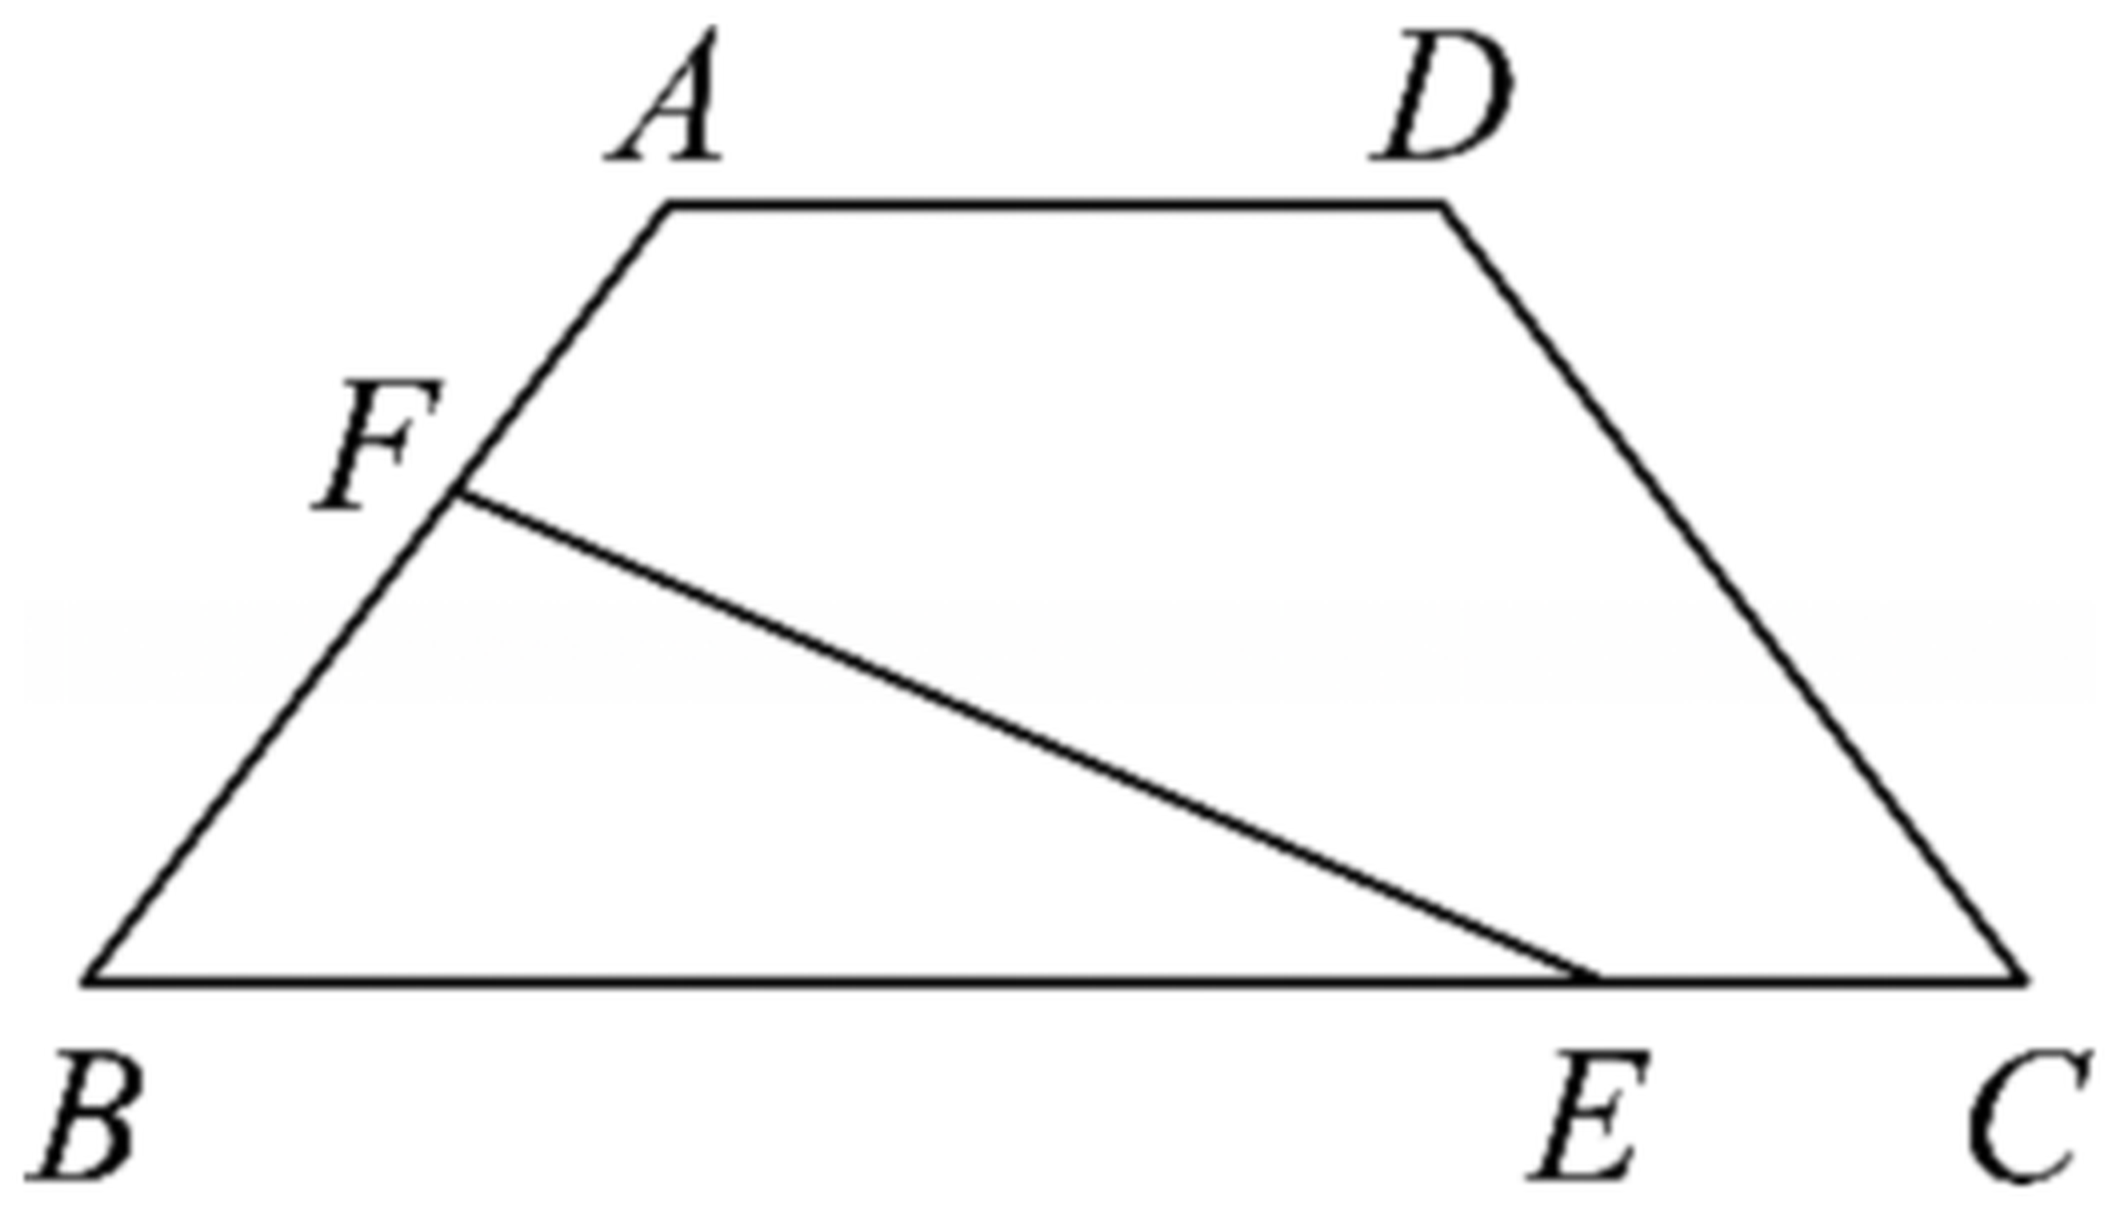
\includegraphics[width=0.46\textwidth]{figures/trapezoid_EF.png}
\end{center}

\begin{enumerate}[label=(\arabic*)]
\item 若 $EF$ 平分等腰梯形 $ABCD$ 的周长，设 $BE$ 长为 $x$，试用含 $x$ 的代数式表示
$\triangle BEF$ 的面积；
\item 是否存在线段 $EF$ 将等腰梯形 $ABCD$ 的周长和面积同时平分？若存在，求出此时 $BE$
的长；若不存在，请说明理由；
\item 是否存在线段 $EF$ 将等腰梯形 $ABCD$ 的周长和面积同时分成 $1:2$ 的两部分？
若存在，求此时 $BE$ 的长；若不存在，请说明理由.
\end{enumerate}

\ifanswer
\solbegin
\stepm{(1)}{过 $A$ 作 $AK\perp BC$ 交 $BC$ 于点 $K$，过 $F$ 作 $FG\perp BC$ 交 $BC$ 于点
$G$，}

\begin{center}
% 图取原卷截图、4× LANCZOS 放大（同梯形，多出虚线 $FG\perp BC$ 与 $AK\perp BC$
% 及两处直角符号；图只在【解析】里出现，故放进 \ifanswer 块）。
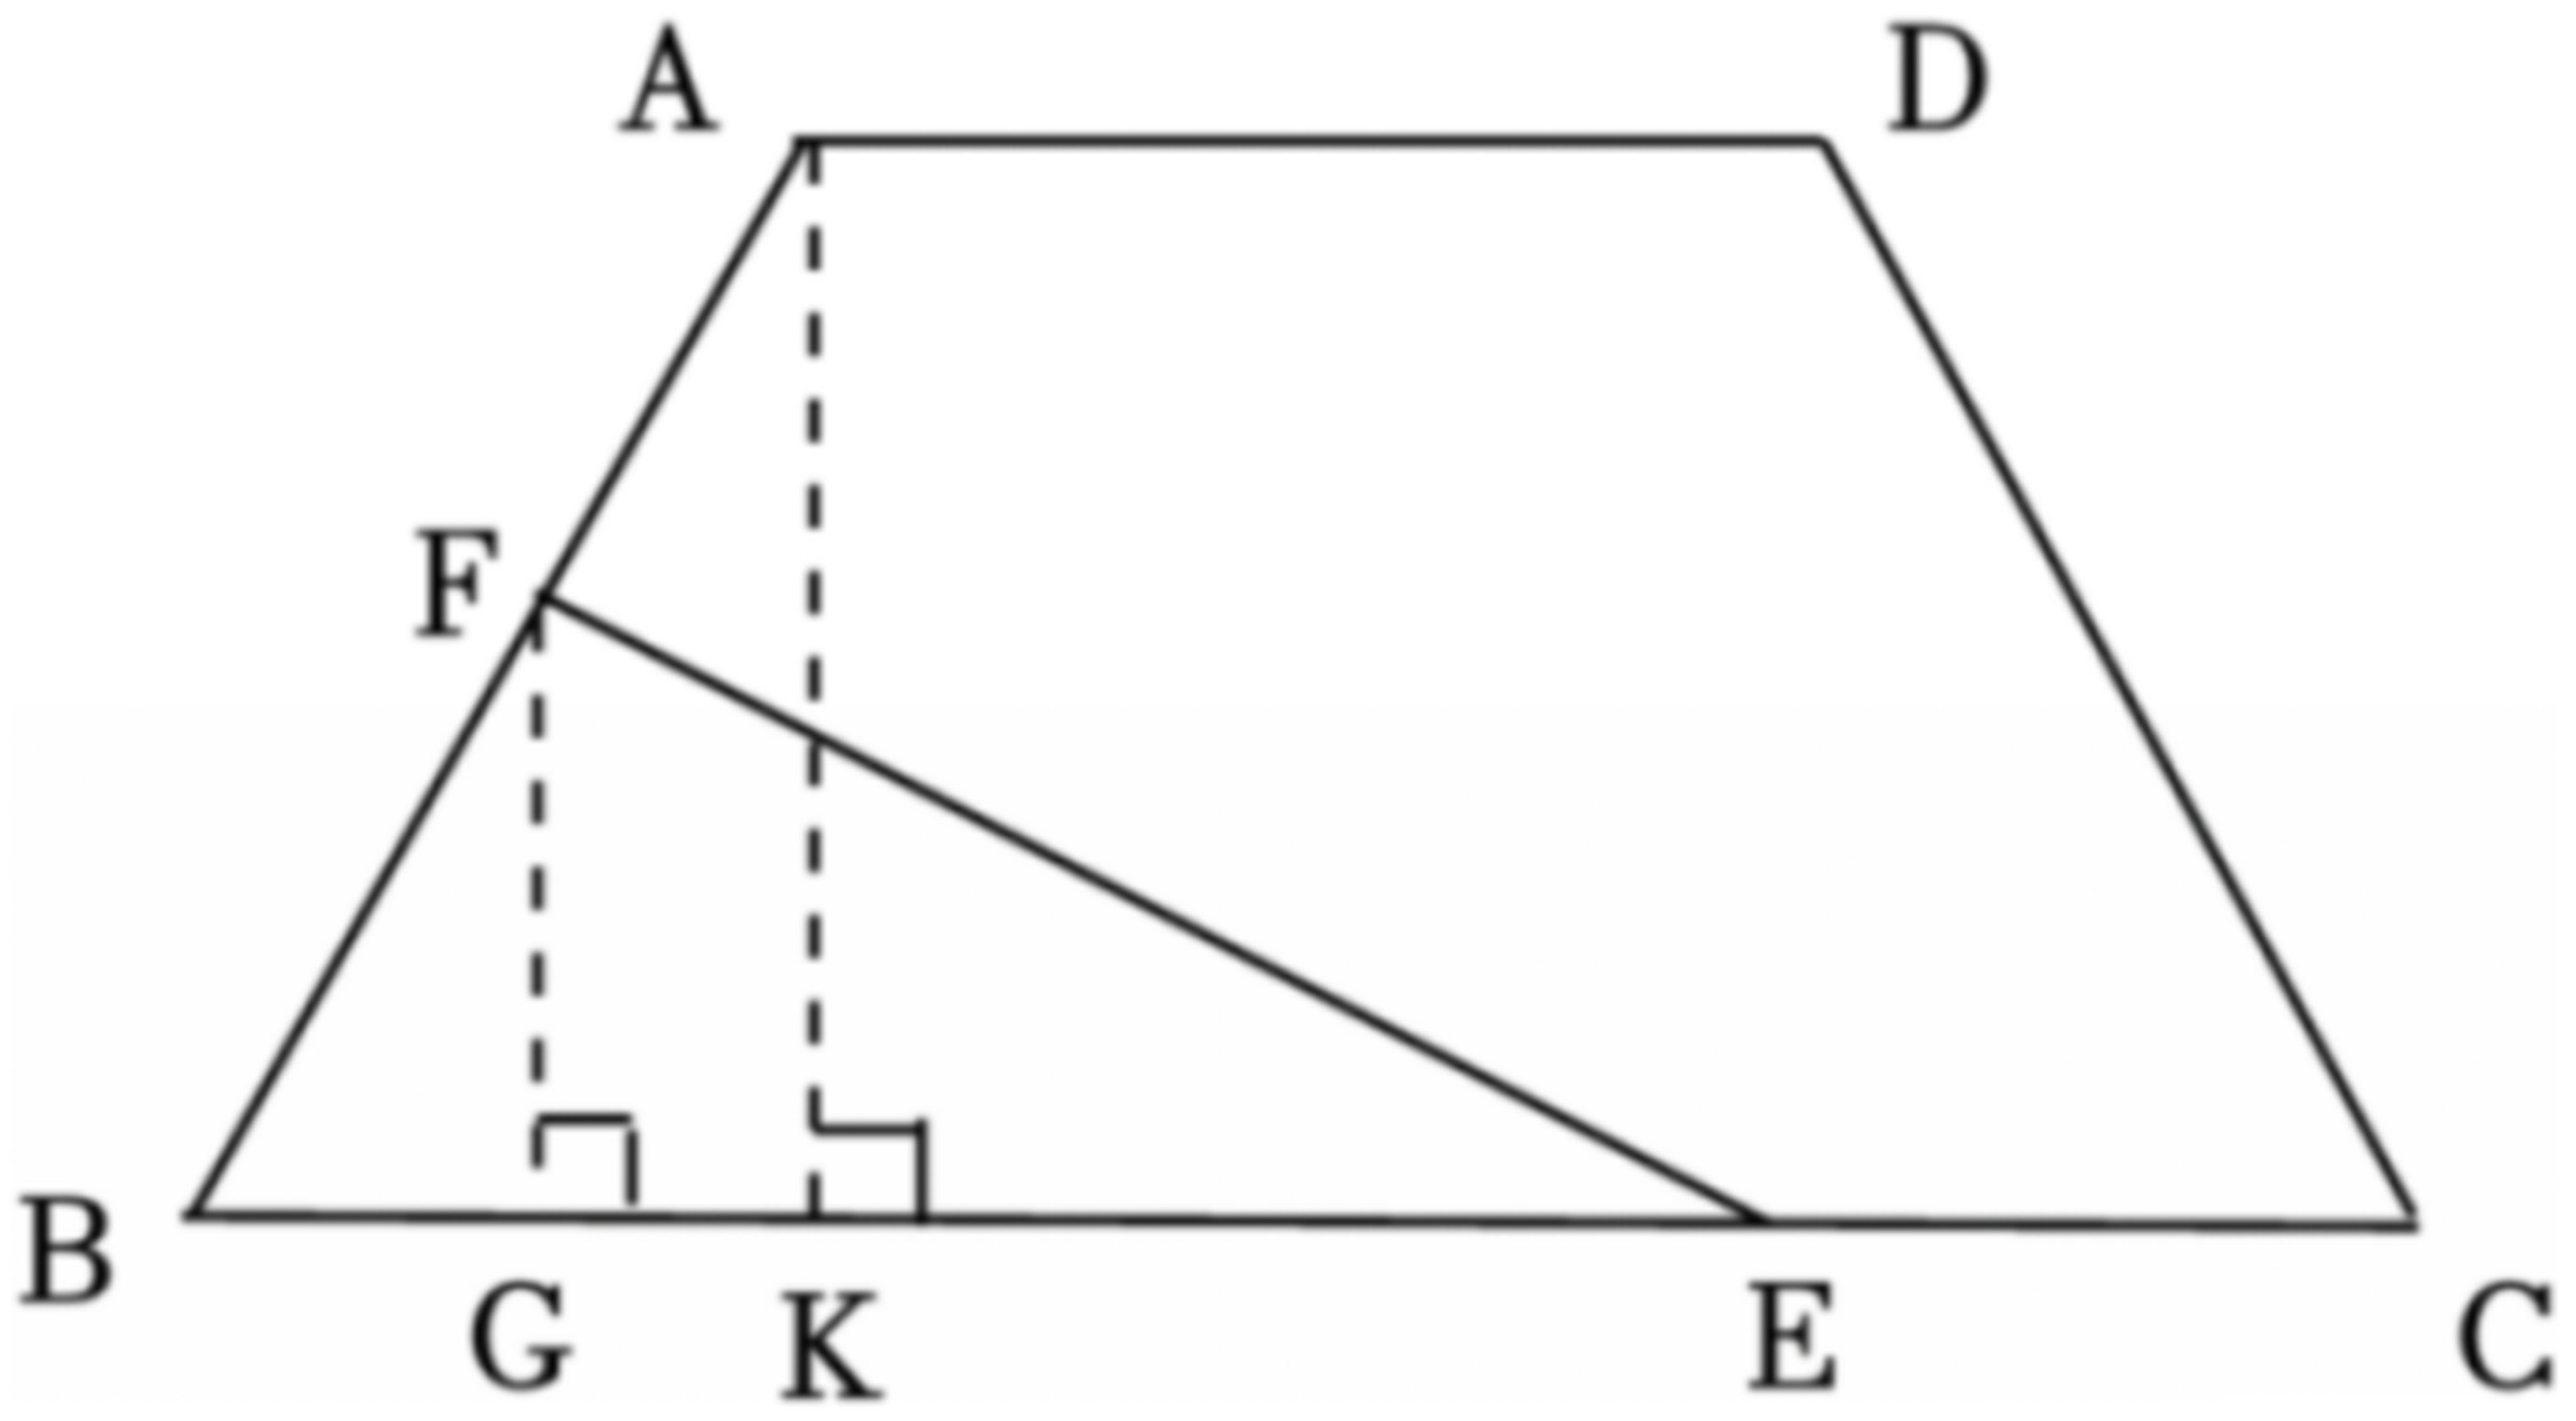
\includegraphics[width=0.62\textwidth]{figures/trapezoid_EF_aux.png}
\end{center}

\step{所以 $BK=\dfrac12\times(BC-AD)=\dfrac12\times(10-4)=3$，}
\step{$AK=\sqrt{AB^2-BK^2}=\sqrt{5^2-3^2}=4$，}
\step{由题意得，梯形 $ABCD$ 周长为 $24$，高为 $4$，面积为 $28$，}
\step{因为 $EF$ 平分等腰梯形 $ABCD$ 的周长，设 $BE$ 长为 $x$，则 $BF=12-x$，}
\step{由 $\begin{cases}0\leqslant12-x\leqslant5\\ 0\leqslant x\leqslant10\end{cases}$，
解得 $7\leqslant x\leqslant10$，}
\step{由题意得 $\triangle BFG\backsim\triangle BAK$，所以 $\dfrac{FG}{AK}=\dfrac{BF}{BA}$，
即 $\dfrac{FG}4=\dfrac{12-x}5$，}
\step{解得 $FG=\dfrac45(12-x)$，}
\step{所以 $S_{\triangle BEF}=\dfrac12BE\cdot FG
=-\dfrac25x^2+\dfrac{24}5x$（$7\leqslant x\leqslant10$）；}
\stepm{(2)}{存在，由 (1) 得 $-\dfrac25x^2+\dfrac{24}5x=\dfrac{28}2$，$x\in[7,10]$，}
\step{即 $x^2-12x+35=0$，解得 $x=7$ 或 $x=5$（舍去），}
\step{所以存在线段 $EF$ 将等腰梯形 $ABCD$ 的周长和面积同时平分，此时 $BE=7$；}
\stepm{(3)}{不存在，}
\step{情况一：$\triangle BEF$ 的面积$:$多边形 $AFECD$ 的面积 $=1:2$，
$(BE+BF):(AF+AD+DC+CE)=1:2$，}
\step{梯形周长的 $\dfrac13$ 是 $\dfrac{24}3=8$，面积的 $\dfrac13$ 是 $\dfrac{28}3$，}
\step{又因为 $BE=x$，所以 $BF=8-x$，}
\step{又因为 $\dfrac{FG}{AK}=\dfrac{BF}{BA}$，即 $\dfrac{FG}4=\dfrac{8-x}5$，
所以 $FG=\dfrac{32-4x}5$，}
\step{所以 $S_{\triangle BEF}=\dfrac12BE\times FG=-\dfrac25x^2+\dfrac{16}5x$，
所以 $\dfrac{28}3=-\dfrac25x^2+\dfrac{16}5x$，}
\step{整理得 $-3x^2+24x-70=0$，此时 $\Delta<0$，无解，故不存在；}
\step{情况二：$\triangle BEF$ 的面积$:$多边形 $AFECD$ 的面积 $=2:1$，
$(BE+BF):(AF+AD+DC+CE)=2:1$，}
\step{梯形周长的 $\dfrac13$ 为 $\dfrac{24}3=8$，面积的 $\dfrac13$ 为 $\dfrac{28}3$，
又 $BE=x$，所以 $BF=16-x$，}
\step{又 $\dfrac{FG}{AK}=\dfrac{BF}{BA}$，即 $\dfrac{FG}4=\dfrac{16-x}5$，
所以 $FG=\dfrac{64-4x}5$，}
\step{所以 $S_{\triangle BEF}=\dfrac12BE\times FG=-\dfrac25x^2+\dfrac{32}5x$，}
\step{所以 $\dfrac{28}3\times2=-\dfrac25x^2+\dfrac{32}5x$，
整理得 $-3x^2+48x-140=0$，}
\step{解得 $x=\dfrac{48+\sqrt{624}}6>10$，$x=\dfrac{48-\sqrt{624}}6<7$，
不符合题意，舍去，故不存在；}
\step{综上所述，不存在线段 $EF$ 将等腰梯形 $ABCD$ 的周长和面积同时分成 $1:2$ 的两部分.}
\solend

\fi

\ansspace[8]

\item 对集合 $\{1,2,\cdots,n\}$ 及其每一个非空子集 $A$，定义一个唯一确定的“交替和”
如下：将 $A$ 中的元素按照递减的次序排列，然后将第一个元素交替地减或加后继的元素所得的
结果，例如，子集 $\{1,2,4,6,9\}$ 的“交替和”是 $9-6+4-2+1=6$，子集 $\{5,6\}$ 的
“交替和”是 $6-5=1$，子集 $\{2\}$ 的交替和是 $2$；定义一个唯一确定的“交替积”如下：
将 $A$ 中的元素按照递减的次序排列，然后将第一个元素交替地除以或乘以后继的数所得的结果，
例如，集合 $\{1,2,4,6,9\}$ 的“交替积”是 $9\div6\times4\div2\times1=3$，
$\{5,6\}$ 的“交替积”是 $6\div5=1.2$，$\{2\}$ 的“交替积”是 $2$.

\begin{enumerate}[label=(\arabic*)]
\item 对于 $\{1,2,3,4,5,6,7,8,9\}$，求其所有子集的“交替和”的总和；
\item 对于 $\{1,2,\cdots,n\}$，求其所有子集的“交替和”的总和；
\item 对于 $\left\{n\mid\dfrac{495}{n+2}\in\N,n\in\Z\right\}$ 求其所有子集的
“交替积”的总和.
\end{enumerate}

\ifanswer
\solbegin
\stepm{(1)}{集合 $\{1,2,3,4,5,6,7,8,9\}$ 的子集中，除去 $\{9\}$ 外还有 $2^9-2$ 个
非空子集，}
\step{把这 $2^9-2$ 个非空子集两两组合后分别计算每一组中“交替和”之和，}
\step{组合原则是设 $A_i=\{9,a_1,a_2,\cdots\}$，$A_i^1=\{a_1,a_2,\cdots\}$，}
\step{集合 $A_i^1$ 的元素为集合 $A_i$ 中去掉 $9$ 的所有元素，把 $A_i$ 和 $A_i^1$
结合为一组，}
\step{显然，每组的“交替和”的和为 $9$，共有 $\dfrac{2^9-2}2$ 组，}
\step{所以，所有“交替和”之和应该为 $\dfrac{9(2^9-2)}2+9=2304$；}
\stepm{(2)}{集合 $\{1,2,\cdots,n\}$ 的子集中，除去 $\{n\}$ 外还有 $2^n-2$ 个非空子集，}
\step{把这 $2^n-2$ 个非空子集两两组合后分别计算每一组中“交替和”之和，}
\step{组合原则是设 $A_i=\{n,a_1,a_2,\cdots\}$，$A_i^1=\{a_1,a_2,\cdots\}$，}
\step{集合 $A_i^1$ 的元素为集合 $A_i$ 中去掉 $n$ 的所有元素，把 $A_i$ 和 $A_i^1$
结合为一组，}
\step{显然，每组的“交替和”的和为 $n$，共有 $\dfrac{2^n-2}2$ 组，}
% 注：下一行分子原卷印作花括号（其余同类处皆用圆括号），照抄未改，见文件头“原卷存疑”③。
\step{所以，所有“交替和”之和应该为 $\dfrac{n\{2^n-2\}}2+n=n\cdot2^{n-1}$；}
\stepm{(3)}{集合 $\left\{n\mid\dfrac{495}{n+2}\in\N,n\in\Z\right\}
=\{493,163,97,53,43,31,13,9,7,3,1,-1\}$，}
\step{其中除去 $\{-1\}$ 外还有 $2^{12}-2$ 个非空子集，}
% 注：下一行原卷把“把这”重复印了一次（“把这把这”），照抄未改，见文件头“原卷存疑”②。
\step{把这把这 $2^{12}-2$ 个非空子集两两组合后分别计算每一组中“交替积”之和，}
\step{组合原则是设 $A_j=\{-1,a_1,a_2,\cdots\}$，$A_j^1=\{a_1,a_2,\cdots\}$，}
\step{集合 $A_j^1$ 的元素为集合 $A_j$ 中去掉 $-1$ 的所有元素，把 $A_j$ 和 $A_j^1$
结合为一组，}
\step{显然，每组的“交替积”的和为 $0$，共有 $\dfrac{2^{12}-2}2$ 组，}
\step{所以，所有“交替积”之和应该为 $\dfrac{2^{12}-2}2\times0-1=-1$.}
\solend

\fi

\ansspace*[10]

\end{enumerate}

\end{document}
"
% 紧凑版：xelatex "\def\iscompact{1}% 高一30_南洋模范中学_开学考.tex
%   —— 高一上数学“2026-2027 年南洋模范中学高一上开学考”（试卷版/答案版）
% 试卷版：xelatex 高一30_南洋模范中学_开学考.tex
% 答案版：xelatex "\def\isanswer{1}\input{高一30_南洋模范中学_开学考.tex}"
% 紧凑版：xelatex "\def\iscompact{1}\input{高一30_南洋模范中学_开学考.tex}"
%
% 原始材料是微信公众号图文（公众号“魔都数学加油站”连载“27学年高一 30”，2026-09-23 发布，
% 原文标题“27学年高一30——2026-2027年上海市南洋模范中学高一上开学考”），
% 正文为 11 张 PNG 页。**同一篇里各页分辨率不一致**——第 2、3、9、10 页 4762×6735，
% 其余七页 2560×3620（已逐页打开确认，非下载缺档），取的是 mmbiz.qpic.cn/<hash>/0 的原图档。
% 原文本身就是一份**讲评版**：填空第 3—7 题下方印【答案】，第 8—12 题与其后各题印【解析】。
% 试题文字、答案与解析均照原卷录入，未改内容。卷面的粉色斜水印属水印，未录入。
%
% 卷首标题：原卷印作“2026-2027 年南洋模范中学高一上开学考”（公众号标题里的“上海市”
% 三字卷面标题行没有，本稿照卷面），年份区间按全稿惯例排 en dash，前缀照原卷保留“年”。
%
% 与原卷的排版差异（均已在 README“说明”中交代）：
%   ① 原文自**第 3 题**起（第 1、2 题未在该文中发布），故本稿题号亦自 3 起；
%   ② 原卷本就印有“一、填空题”“二、选择题”“三、解答题”三节标题，本稿照原卷分节，
%      只把标题改排成全稿统一的“大节标题”样式；
%   ③ 原卷填空第 3—7 题只印【答案】行、第 8 题起印【解析】（选择题答案写在解析末句
%      “故选 D／B”里），本稿统一改为试卷版隐去、答案版以 \ans{}／\ifanswer 块给出，
%      两版彻底分离；
%   ④ 子集符号原卷两种并用：第 7 题题干两处、第 19(2) 题作带下划线的 $\subseteq$，
%      第 17(2) 题解析作真包含的 $\subset$，本稿分别照录为 $\sub$ 与 $\subset$；
%   ⑤ 补集符号原卷一律作**上横线**（$\overline{A}$、$\overline{B}$），本稿照录；
%   ⑥ 原卷的实数集 R 一律作斜体（第 4 题、第 17 题与第 19 题题干的 $U=R$），
%      第 21(3) 题的自然数集与整数集作**粗体** $\mathbf{N}$、$\mathbf{Z}$，
%      本稿按全稿惯例统一写作 $\R$、$\N$、$\Z$；
%   ⑦ 原卷填空的横线约两个字宽，本稿按全稿惯例统一排 \blankline[4.4em]；
%   ⑧ 原卷未印副标题，本稿按全稿惯例补出副标题“集合与常用逻辑用语”——但本卷是开学考，
%      范围不止这一章：第 18 题是速度—时间图象题、第 20 题是等腰梯形的周长/面积平分问题，
%      副标题只标了主章节（见文末“高一30 专记”）；
%   ⑨ 第 13、14、18、20 题的图印在题干右侧、第 16 题的三幅图印在【解析】里的下一页顶部、
%      第 20 题【解析】另有一张带辅助线的图，本稿一律移至题干或解析之后；
%      图取原卷截图、4× LANCZOS 放大（见各 \includegraphics 前的注释）。
%
% 原卷存疑三处（均照抄原卷、未改，见源码中该处上方注释）：
%   ① 第 10 题【解析】验证“破晓集”时写的是 $\notin A$、$\in A$（如“$-2-2=-4\notin A$”），
%      但该处讨论的集合原题设里叫 $P$，同题②的“$x+y=2(k_1+k_2)\in A$”亦然——
%      本稿照抄未改（按文意应为 $P$）；
%   ② 第 21 题【解析】(3) 有“把这把这 $2^{12}-2$ 个非空子集”（“把这”重复印了一次）；
%   ③ 同题 (2) 的结论式分子原卷印作花括号 $\dfrac{n\{2^n-2\}}{2}$（其余同类处皆用圆括号）。

\documentclass[a4paper,11pt]{article}
\usepackage{common}

\begin{document}

\examtitlest[3]{2026--2027 年南洋模范中学高一上开学考}{集合与常用逻辑用语}

\bigsec{一、填空题}

\begin{enumerate}
\setcounter{enumi}{2}

\item 若集合 $A=\{x\mid x^2-2kx+7k=0\}$ 有且仅有三个真子集，则 $k$ 的取值范围是
\blankline[4.4em].

\ans{$(-\infty,0)\cup(7,+\infty)$}

\item “存在 $x\in\R$，使得 $x^2+2x+5=0$”的否定形式是 \blankline[4.4em].

\ans{对任何 $x\in\R$，都有 $x^2+2x+5\neq0$}

\item 下列命题中，$p$ 是 $q$ 的必要非充分条件的是 \blankline[4.4em].

① $p:x>2$ 且 $y>3$，$q:x+y>5$；

② $p$：四边形的四个角都相等，$q$：四边形是正方形.

\ans{②}

\item 若“条件 $\alpha:2\leqslant x\leqslant4$”是“条件 $\beta:3m-1\leqslant x\leqslant-m$”的
充分非必要条件，则 $m$ 的取值范围是 \blankline[4.4em].

\ans{$(-\infty,-4]$}

\item 满足 $\{1\}\sub M\sub\{1,2,4,5\}$ 的集合 $M$ 的个数为 \blankline[4.4em] 个.

\ans{$8$}

\item 已知集合 $A=\{1,2\}$，集合 $B=\{x\mid ax=6\}$，若 $A\cup B=A$，则 $a$ 的所有取值
构成的集合为 \blankline[4.4em].

\ifanswer
\solbegin
\step{因为 $A\cup B=A$，所以 $B\sub A$，}
\step{当 $a=0$ 时，$B=\varnothing$，满足 $B\sub A$；}
\step{当 $a\neq0$ 时，$B=\left\{\dfrac6a\right\}$，则 $\dfrac6a=1$ 或 $\dfrac6a=2$，
解得 $a=6$ 或 $a=3$，}
\step{综上所述，$a$ 的所有取值构成的集合为 $\{0,3,6\}$.}
\solend

\fi

\item 对于集合 $M$、$N$，定义 $M-N=\{x\mid x\in M\text{ 且 }x\notin N\}$，
$M\oplus N=(M-N)\cup(N-M)$，设 $A=\{y\mid y=|x|,x\in\R\}$，
$B=\{y\mid y=-(x-1)^2+2,x\in\R\}$，则 $A\oplus B=$ \blankline[4.4em].

\ifanswer
\solbegin
\step{由已知 $A=[0,+\infty)$，$B=(-\infty,2]$，}
\step{由于 $A-B=(2,+\infty)$，$B-A=(-\infty,0)$，}
\step{故 $A\oplus B=(A-B)\cup(B-A)=(-\infty,0)\cup(2,+\infty)$.}
\solend

\fi

\item 设 $P$ 为非空实数集满足：对任意给定的 $x$、$y\in P$（$x$、$y$ 可以相同），都有
$x+y\in P$，$x-y\in P$，$xy\in P$，则称 $P$ 为破晓集. 关于破晓集有下列结论：
①集合 $P=\{-2,-1,0,1,2\}$ 为破晓集；②集合 $P=\{x\mid x=2n,n\in\Z\}$ 为破晓集；
③若集合 $P_1$、$P_2$ 为破晓集，则 $P_1\cup P_2$ 为破晓集；④若集合 $P$ 为破晓集，
则一定有 $0\in P$；⑤若集合 $P_1$、$P_2$ 为破晓集，则 $P_1\cap P_2$ 为破晓集；
其中正确结论的序号是 \blankline[4.4em].

\ifanswer
\solbegin
% 注：以下几步原卷把该集合记作 $A$（题设里叫 $P$），照抄未改，见文件头“原卷存疑”①。
\step{对于①：$-2-2=-4\notin A$，故集合 $P=\{-2,-1,0,1,2\}$ 不为破晓集，故①错误；}
\step{②设 $x$、$y\in A$，则 $x=2k_1$，$y=2k_2$，且 $k_1$、$k_2\in\Z$，}
\step{故 $x+y=2(k_1+k_2)\in A$，$x-y=2(k_1-k_2)\in A$，$xy=4k_1k_2\in A$，}
\step{故集合 $P=\{x\mid x=2n,n\in\Z\}$ 为破晓集，故②正确；}
\step{③若集合 $P_1$、$P_2$ 为破晓集，设 $P_1=\{x\mid x=2k,k\in\Z\}$，
$P_2=\{x\mid x=3k,k\in\Z\}$，}
\step{但是 $P_1\cup P_2$ 不为破晓集，如 $x=2$，$y=3$ 时，$x+y=5$，
故 $5\notin(P_1\cup P_2)$，故③错误；}
\step{④若集合 $P$ 为破晓集，则取 $x=y$，$x-y=0\in A$，则一定有 $0\in P$，故④正确.}
\step{⑤正确；}
\step{故正确的是②④⑤.}
\solend

\fi

\item 已知集合 $M$ 的元素均为正整数，定义集合 $M$ 的“变项和”为：将 $M$ 中每个元素 $m$
都乘以 $(-1)^m$ 后再求和. 若集合 $A=\{n\mid1\leqslant n\leqslant10,n\in\N\}$，则集合 $A$
的所有非空子集的“变项和”的总和为 \blankline[4.4em].

\ifanswer
\solbegin
\step{$A$ 集合的所有非空子集中，每个元素出现的次数都是
$(2^{10}-1)-(2^9-1)=2^9$，}
\step{则集合 $A$ 的所有非空子集的“变项和”的总和为
$1\times(-1)^1\times2^9+2\times(-1)^2\times2^9+\cdots+10\times(-1)^{10}\times2^9$}
\step{$=(-1+2-3+4-\cdots-9+10)\times2^9=5\times2^9=2560$.}
\solend

\fi

\item 已知集合 $A=[t,t+1]\cup[t+4,t+9]$，$0\notin A$，存在正数 $\lambda$，使得对任意
$a\in A$，都有 $\dfrac\lambda a\in A$，则 $t$ 的值是 \blankline[4.4em].

\ifanswer
\solbegin
\step{当 $t>0$ 时，当 $a\in[t,t+1]$ 时，$\dfrac\lambda a\in[t+4,t+9]$，}
\step{当 $a\in[t+4,t+9]$ 时，$\dfrac\lambda a\in[t,t+1]$，}
\step{即当 $a=t$ 时，$\dfrac\lambda a\leqslant t+9$；当 $a=t+9$ 时，
$\dfrac\lambda a\geqslant t$，即 $\lambda=t(t+9)$；}
\step{当 $a=t+1$ 时，$\dfrac\lambda a\geqslant t+4$，当 $a=t+4$ 时，
$\dfrac\lambda a\leqslant t+1$，即 $\lambda=(t+1)(t+4)$，}
\step{所以 $t(t+9)=(t+1)(t+4)$，解得 $t=1$.}
\step{当 $t+1<0<t+4$ 时，当 $a\in[t,t+1]$ 时，$\dfrac\lambda a\in[t,t+1]$.}
\step{当 $a\in[t+4,t+9]$ 时，则 $\dfrac\lambda a\in[t+4,t+9]$，}
\step{即当 $a=t$ 时，$\dfrac\lambda a\leqslant t+1$，当 $a=t+1$ 时，
$\dfrac\lambda a\geqslant t$，即 $\lambda=t(t+1)$，}
\step{即当 $a=t+4$ 时，$\dfrac\lambda a\leqslant t+9$，当 $a=t+9$ 时，
$\dfrac\lambda a\geqslant t+4$，即 $\lambda=(t+4)(t+9)$，}
\step{所以 $t(t+1)=(t+4)(t+9)$，解得 $t=-3$.}
\step{当 $t+9<0$ 时，同理可得无解.}
\step{综上，$t$ 的值为 $1$ 或 $-3$.}
\solend

\fi

\end{enumerate}

\bigsec{二、选择题}

\begin{enumerate}
\setcounter{enumi}{12}

% 这道题是“题干 + 图 + 选项”约 6cm 的一整块，页末放不下就会被拆开（切页审计的 A 类），
% 故在题前先量一次页高：不够就把整道题干连图带选项一起挪到次页。
\needvspace{6.5cm}
\item 设 $U=\{1,2,3,4,5\}$，$A$、$B$ 都是 $U$ 的子集，且 $A\cap B=\{5\}$，
$\overline{A}\cap B=\{4\}$，$\overline{A}\cap\overline{B}=\{1,2\}$，
则以下四个判断中正确的是\mbox{（\quad）}

\begin{center}
% 图取原卷截图、4× LANCZOS 放大（原卷把图印在题干右侧，本稿移至此处，见文件头⑨）。
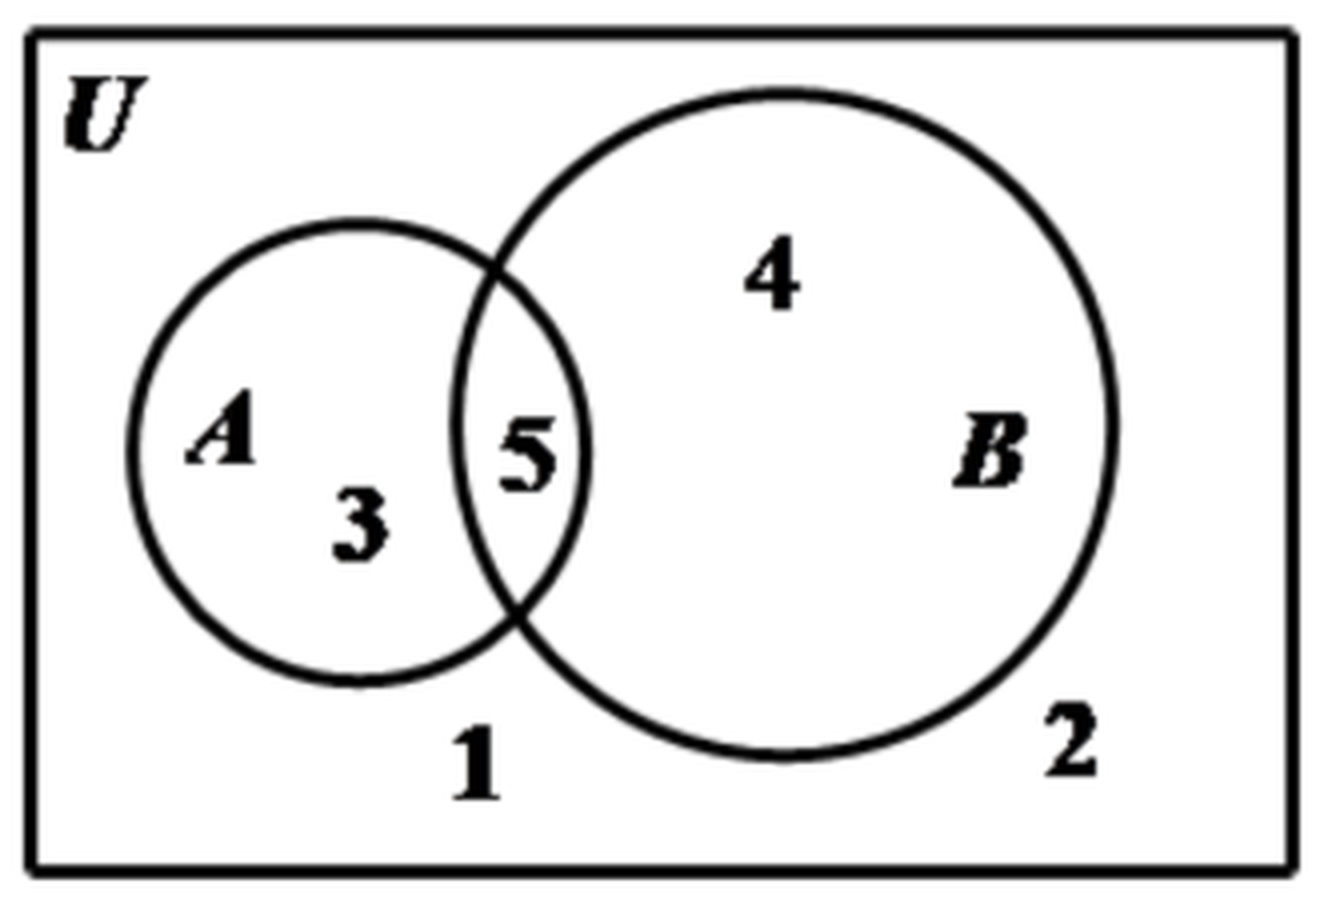
\includegraphics[width=0.28\textwidth]{figures/venn_U5_AB.png}
\end{center}

\keepwithprev
A. $3\notin A$ 且 $3\notin B$\qquad\qquad B. $3\in A$ 且 $3\in B$

C. $3\notin A$ 且 $3\in B$\qquad\qquad D. $3\in A$ 且 $3\notin B$

\ans{$D$}

\ifanswer
\solbegin
\step{画出韦恩图，得 $A=\{5,3\}$，$B=\{5,4\}$，}
\step{则 $3\in A$ 且 $3\notin B$. 故选 $D$.}
\solend

\fi

% 同第 13 题：整块（题干 + 图 + 选项）在答案版还要再挂【答案】【解析】，页末更易被拆开。
\needvspace{7.5cm}
\item 如图表示图形阴影部分的是\mbox{（\quad）}

\begin{center}
% 图取原卷截图、4× LANCZOS 放大（三圆 $A$、$B$、$C$，阴影为整个 $A$ 圆加 $B\cap C$）。
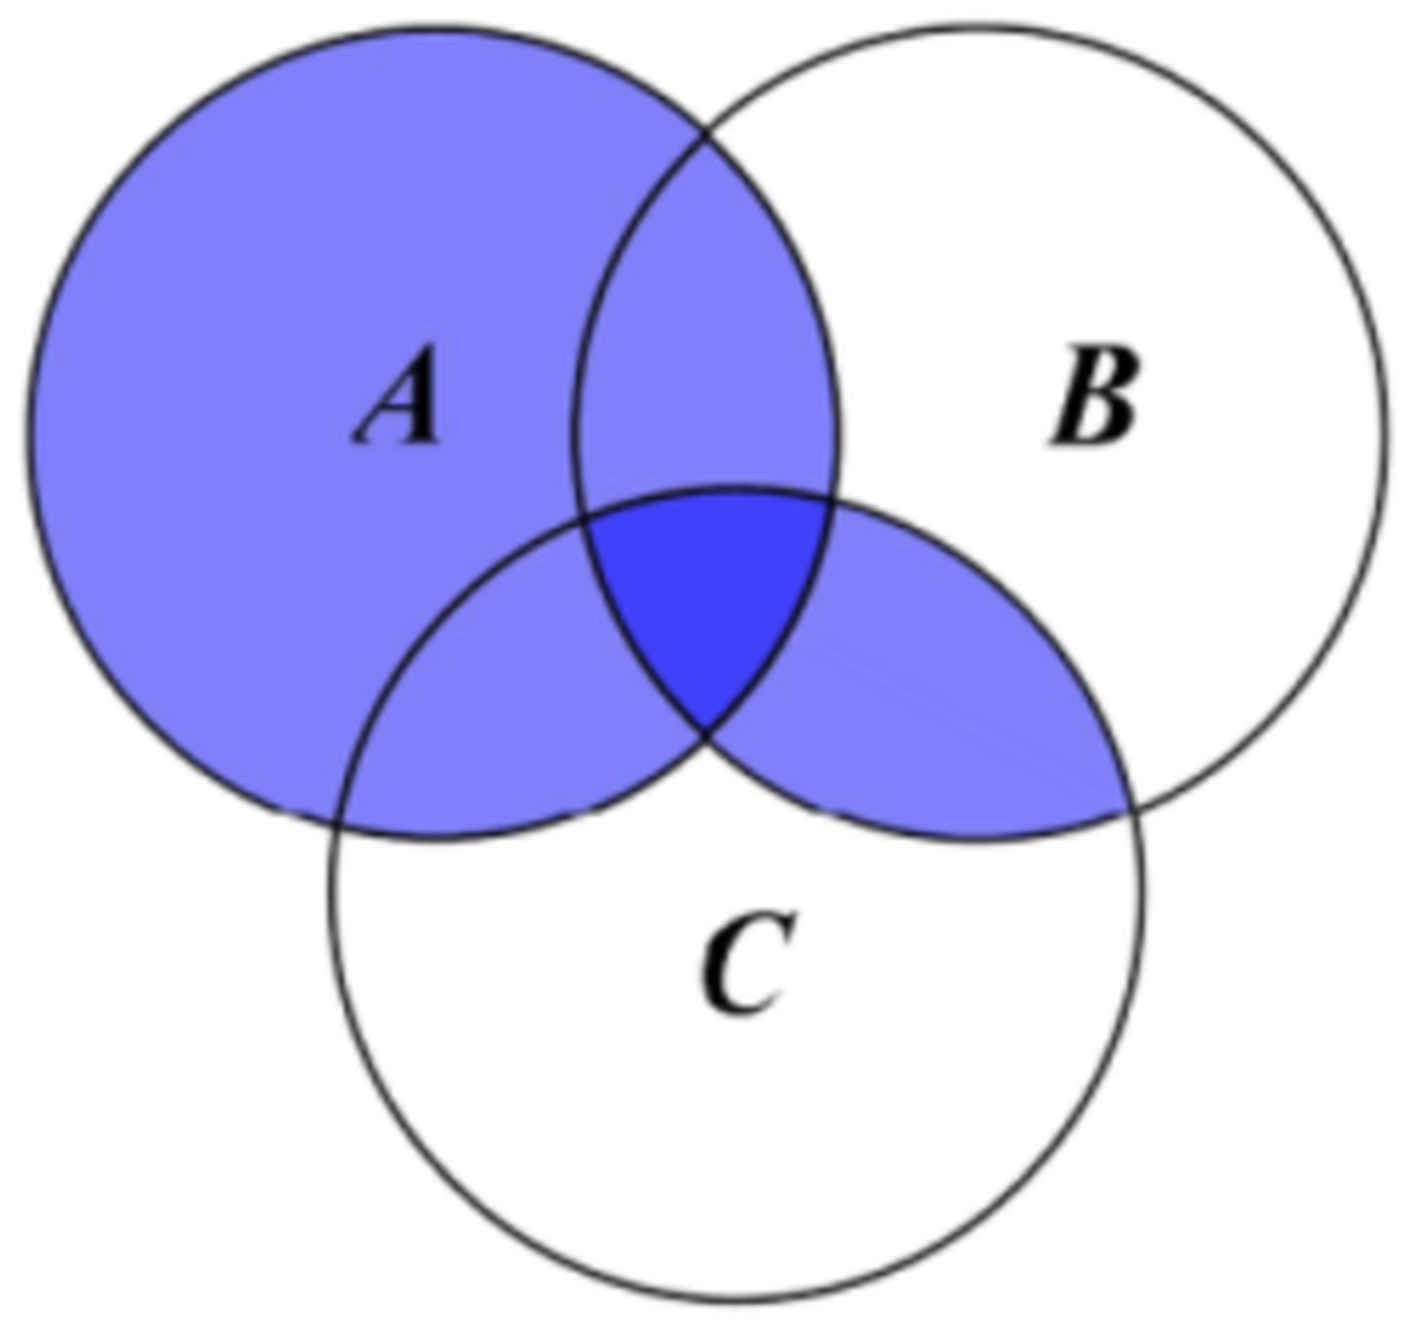
\includegraphics[width=0.30\textwidth]{figures/venn_A_union_BC.png}
\end{center}

\keepwithprev
A. $(A\cup C)\cap(B\cup C)$\qquad\qquad B. $(A\cup B)\cap(A\cup C)$

C. $(A\cup B)\cap(B\cup C)$\qquad\qquad D. $(A\cup B)\cap C$

\ans{$B$}

\ifanswer
\solbegin
\step{图中阴影部分表示元素满足是 $A$ 中的元素，或者是 $B$ 与 $C$ 的公共元素，}
\step{故可以表示为 $A\cup(B\cap C)$，也可以表示为 $(A\cup B)\cap(A\cup C)$.
故选 $B$.}
\solend

\fi

\item 设集合 $M=\left\{x\mid m\leqslant x\leqslant m+\dfrac34\right\}$，
$N=\left\{x\mid n-\dfrac13\leqslant x\leqslant n\right\}$，且 $M$、$N$ 都是集合
$\{x\mid0\leqslant x\leqslant1\}$ 的子集，如果把 $b-a$ 叫做集合
$\{x\mid a\leqslant x\leqslant b\}$ 的“长度”，那么集合 $M\cap N$ 的“长度”的
最小值是\mbox{（\quad）}

\keepwithprev
A. $\dfrac23$\qquad B. $\dfrac1{12}$\qquad C. $\dfrac13$\qquad D. $\dfrac5{12}$

\ans{$B$}

\ifanswer
\solbegin
\step{$M$ 的长度为 $\dfrac34$，$N$ 的长度为 $\dfrac13$，}
\step{当集合 $M\cap N$ 的长度的最小值时，$M$ 与 $N$ 应分别在区间 $[0,1]$ 的左右两端，}
\step{故 $M\cap N$ 的长度的最小值是 $\dfrac34+\dfrac13-1=\dfrac1{12}$，故选 $B$.}
\solend

\fi

\item 定义集合运算 $A-B=\{x\mid x\in A\text{ 且 }x\notin B\}$ 称为集合 $A$ 与集合 $B$ 的
差集；定义集合运算 $A\Delta B=(A-B)\cup(B-A)$ 称为集合 $A$ 与集合 $B$ 的对称差，
有以下 $4$ 个等式：① $A\Delta B=B\Delta A$；② $(A\Delta B)\Delta C=A\Delta(B\Delta C)$；
③ $A\cap(B\Delta C)=(A\cap B)\Delta(A\cap C)$；
④ $A\cup(B\Delta C)=(A\cup B)\Delta(A\cup C)$，
则 $4$ 个等式中恒成立的是\mbox{（\quad）}

\keepwithprev
A. ①②\qquad B. ①②③\qquad C. ①②④\qquad D. ①②③④

\ans{$B$}

\ifanswer
\solbegin
\step{对于①，由 $B\Delta A=(B-A)\cup(A-B)=(A-B)\cup(B-A)=A\Delta B$，
所以①正确；}
\step{对于②，由 $A-B=\{x\mid x\in A\text{ 且 }x\notin B\}
=\{x\mid x\in A,x\notin(A\cap B)\}=A-(A\cap B)$，}
\step{同理可得 $B-A=B-(A\cap B)$，}
\step{则 $A\Delta B=(A-B)\cup(B-A)=(A\cup B)-(A\cap B)$，}
\step{所以 $(A\Delta B)\Delta C=(A\Delta B)\cup C-(A\Delta B)\cap C$，}
\step{所以表示的集合为图（1）中阴影部分所表示的集合，如图所示，}
\step{同理 $A\Delta(B\Delta C)=A\cup(B\Delta C)-A\cap(B\Delta C)$，
也表示图（1）中阴影部分所表示的集合，}
\step{所以 $(A\Delta B)\Delta C=A\Delta(B\Delta C)$，所以②正确；}

\begin{center}
% 图取原卷截图、4× LANCZOS 放大（原卷印在下一页顶部，共三幅三圆韦恩图：
% 图（1）一幅、图（2）左右两幅，图（2）两幅下方各有一行式子标注）。
% 图只在【解析】里出现，故放进 \ifanswer 块，试卷版不排。
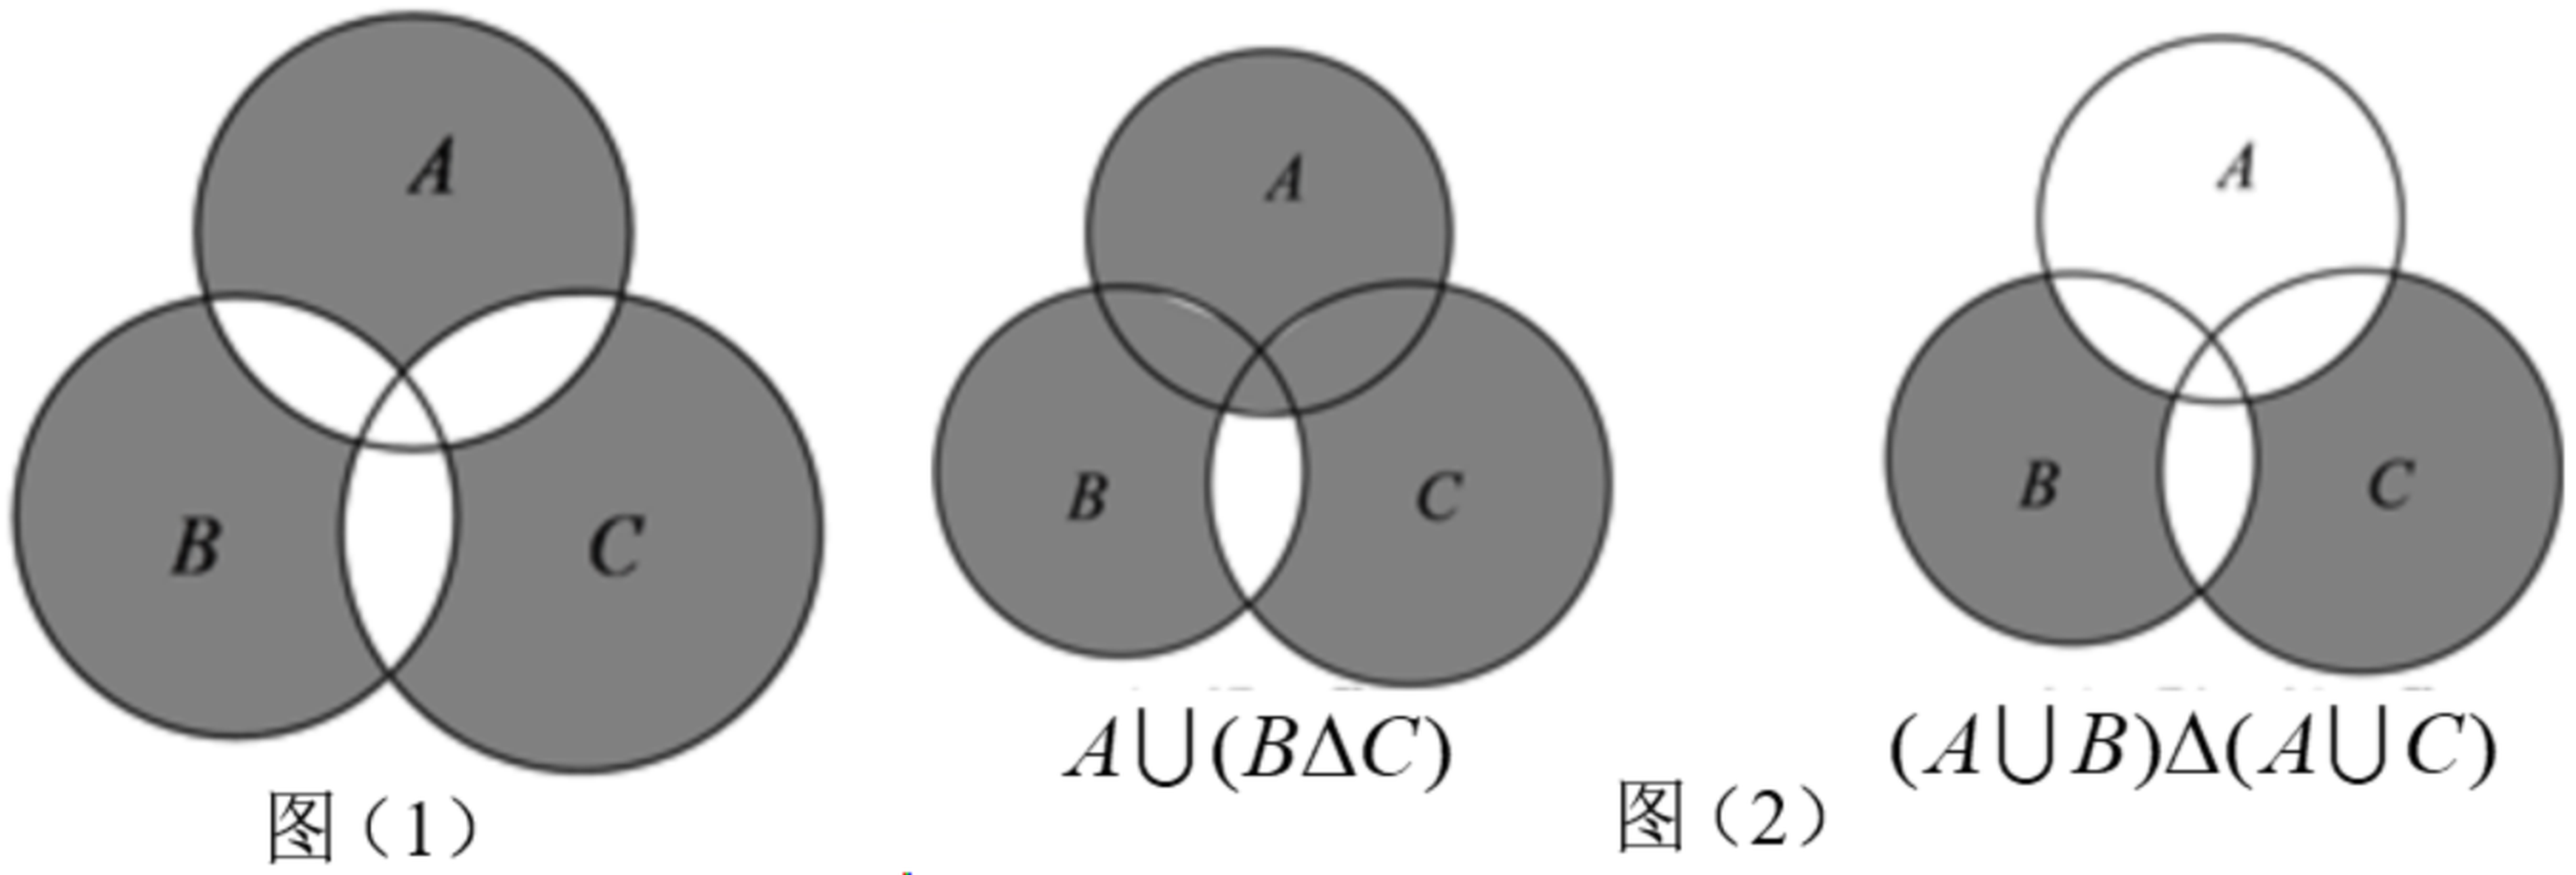
\includegraphics[width=0.86\textwidth]{figures/venn_symdiff3.png}
\end{center}

\step{对于③，由 $A\cap(B\Delta C)=A\cap(B\cup C-B\cap C)
=A\cap(B\cup C)-A\cap(B\cap C)$}
\step{$=(A\cap B)\cup(A\cap C)-(A\cap B)\cap(A\cap C)=(A\cap B)\Delta(A\cap C)$，
所以③正确；}
\step{对于④，如图（2）所示，$A\cup(B\Delta C)\neq(A\cup B)\Delta(A\cup C)$，
所以④错误.}
\step{故选 $B$.}
\solend

\fi

\end{enumerate}

\bigsec{三、解答题}

\begin{enumerate}
\setcounter{enumi}{16}

\item 已知集合 $M=\{x\mid a-1\leqslant x\leqslant2a+3\}$，$P=\{x\mid-2<x\leqslant4\}$，
全集 $U=\R$.

\begin{enumerate}[label=(\arabic*)]
\item 当 $a=2$ 时，求 $M\cap P$；
\item 若 $x\in P$ 是 $x\in M$ 的必要不充分条件，求实数 $a$ 的取值范围.
\end{enumerate}

\ifanswer
\solbegin
\stepm{(1)}{当 $a=2$ 时，集合 $M=\{x\mid1\leqslant x\leqslant7\}$，}
\step{所以 $M\cap P=\{x\mid1\leqslant x\leqslant4\}$；}
\stepm{(2)}{因为 $x\in P$ 是 $x\in M$ 的必要不充分条件，所以 $M\subset P$，}
\step{当 $M=\varnothing$ 时，$a-1>2a+3$，解得 $a<-4$，}
\step{当 $M\neq\varnothing$ 时，则
$\begin{cases}a-1\leqslant2a+3\\ a-1>-2\\ 2a+3\leqslant4\end{cases}$，
解得 $-1<a\leqslant\dfrac12$，}
\step{综上所述，实数 $a$ 的取值范围为
$(-\infty,-4)\cup\left(-1,\dfrac12\right]$.}
\solend

\fi

\ansspace[6]

\item 一辆汽车在某段路程中的行驶速度与时间的关系如图：

\begin{center}
% 图取原卷截图、4× LANCZOS 放大（速度—时间图：纵轴 $v/(\mathrm{km/h})$、
% 横轴 $t(\mathrm{h})$，$t\in[0,1]$、$[1,2]$、$[2,3]$ 三段矩形条高 50、80、90）。
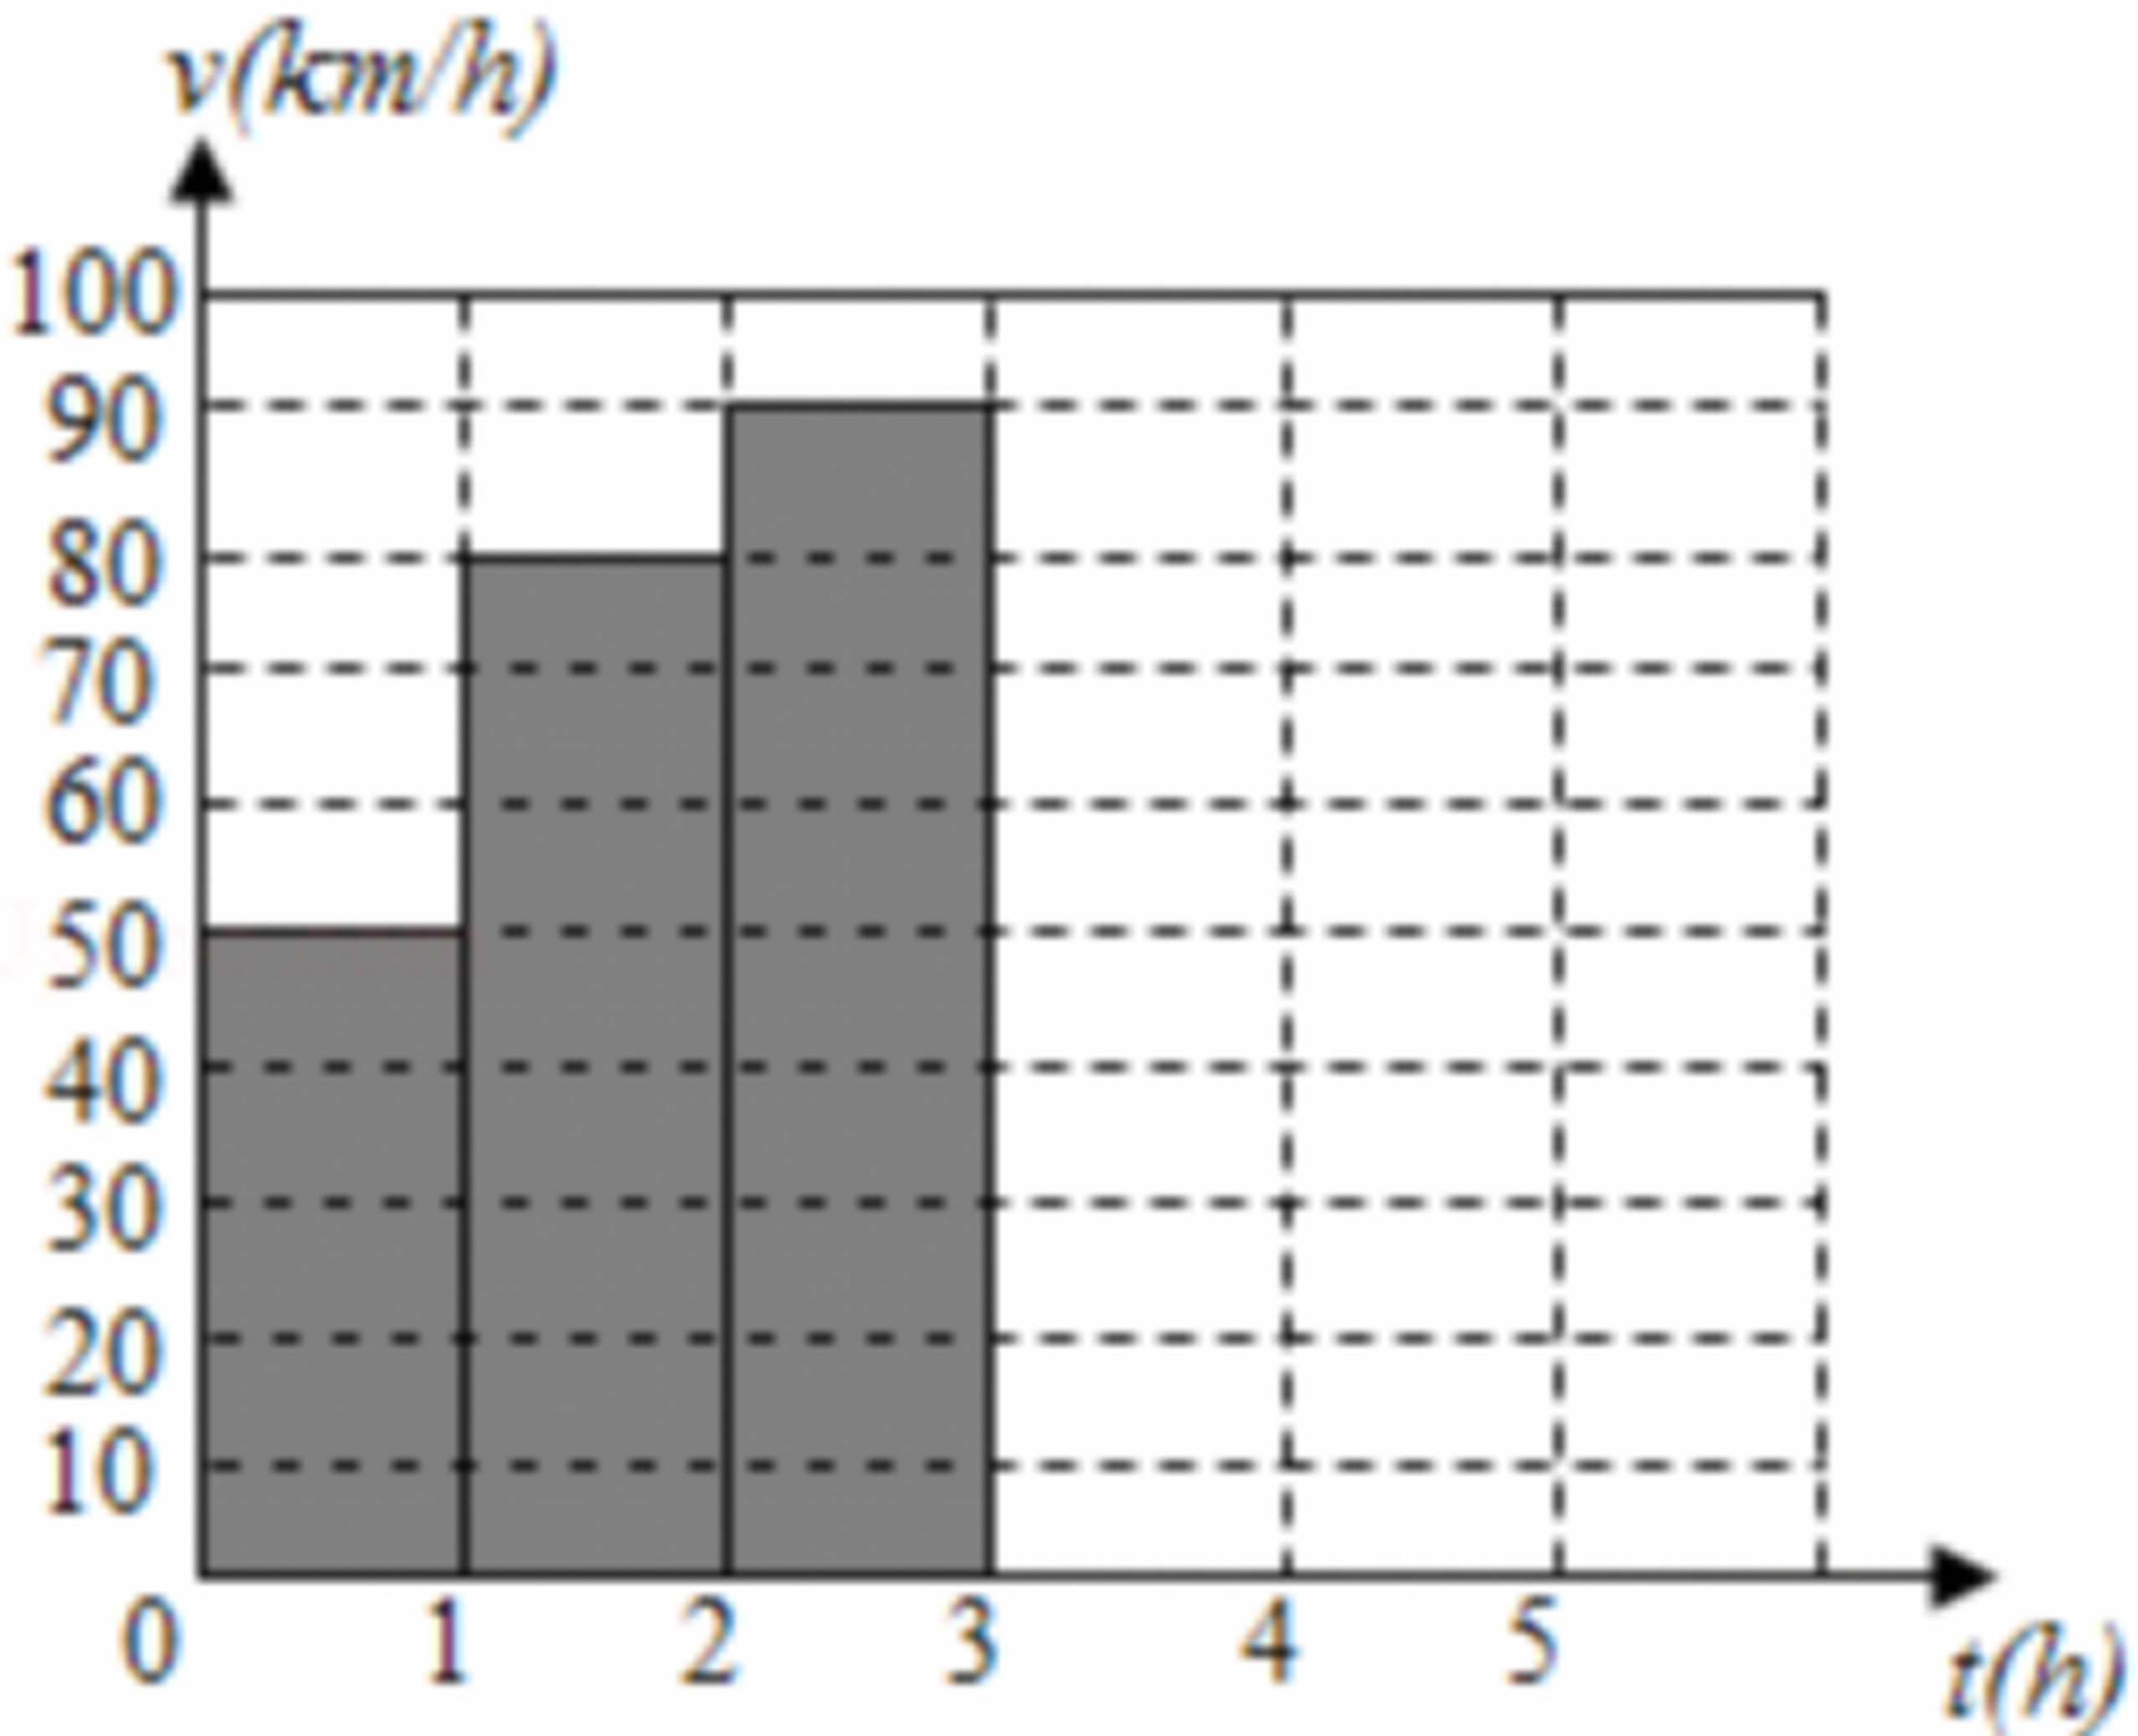
\includegraphics[width=0.52\textwidth]{figures/speed_time_bars.png}
\end{center}

\begin{enumerate}[label=(\arabic*)]
\item 求图中阴影部分的面积，并说明所求面积的实际意义；
\item 假设这辆汽车的里程表在汽车行驶这段路程前的读数为 $2004\,\mathrm{km}$，
试将汽车行驶这段路程时汽车里程表读数 $S$ 表示为时间 $t$ 的函数，
并求出当汽车里程表读数为 $2094\,\mathrm{km}$ 时，汽车行驶了多少时间？
\end{enumerate}

\ifanswer
\solbegin
\stepm{(1)}{由一辆汽车在某段路程中的行驶速度与时间的关系图，}
\step{得阴影部分的面积为 $50\times1+80\times1+90\times1=220$，}
\step{阴影部分的面积表示汽车在 $3$ 小时内行驶的路程为 $220\,\mathrm{km}$.}
\stepm{(2)}{$S=\begin{cases}
50t+2004,&0\leqslant t<1\\
80(t-1)+2054,&1\leqslant t<2\\
90(t-2)+2134,&2\leqslant t\leqslant3
\end{cases}$}
\step{令 $80(t-1)+2054=2094$，解得 $t=1.5$，所以汽车行驶 $1.5$ 小时.}
\solend

\fi

\ansspace[6]

\item 已知集合 $A=\{x\mid x<-2\text{ 或 }x\geqslant3\}$，$U=\R$.

\begin{enumerate}[label=(\arabic*)]
\item 求 $\overline{A}$；
\item 若 $B=\{x\mid mx-1>0\}$，当 $B\sub A$ 时，求实数 $m$ 的取值范围；
\item 若 $B=\{x\mid2m-6\leqslant x\leqslant m+4\}$，当 $B\cap\overline{A}=\varnothing$ 时，
求实数 $m$ 的取值范围.
\end{enumerate}

\ifanswer
\solbegin
\stepm{(1)}{因为集合 $A=\{x\mid x<-2\text{ 或 }x\geqslant3\}$，$U=\R$，
所以 $\overline{A}=\{x\mid-2\leqslant x<3\}$；}
\stepm{(2)}{当 $m=0$ 时，$B=\varnothing$，符合题意，}
\step{当 $m>0$ 时，$B=\left\{x\mid x>\dfrac1m\right\}$，则 $\dfrac1m\geqslant3$，
解得 $0<m\leqslant\dfrac13$，}
\step{当 $m<0$ 时，$B=\left\{x\mid x<\dfrac1m\right\}$，则 $\dfrac1m\leqslant-2$，
解得 $-\dfrac12\leqslant m<0$，}
\step{综上所述，实数 $m$ 的取值范围 $\left[-\dfrac12,\dfrac13\right]$；}
\stepm{(3)}{由题意得 $B=\{x\mid2m-6\leqslant x\leqslant m+4\}$，
$\overline{A}=\{x\mid-2\leqslant x<3\}$，且 $B\cap\overline{A}=\varnothing$，}
\step{当 $B=\varnothing$ 时，$2m-6>m+4$，解得 $m>10$，}
\step{当 $B\neq\varnothing$ 时，则 $\begin{cases}2m-6\leqslant m+4\\ m+4<-2\end{cases}$
或 $\begin{cases}2m-6\leqslant m+4\\ 2m-6\geqslant3\end{cases}$，}
\step{解得 $m<-6$ 或 $\dfrac92\leqslant m\leqslant10$，}
\step{综上所述，实数 $m$ 的取值范围为
$(-\infty,-6)\cup\left[\dfrac92,+\infty\right)$.}
\solend

\fi

\ansspace[8]

\item 在等腰梯形 $ABCD$ 中，$AB=DC=5$，$AD=4$，$BC=10$. 点 $E$ 在下底边 $BC$ 上.
点 $F$ 在腰 $AB$ 上.

\begin{center}
% 图取原卷截图、4× LANCZOS 放大（等腰梯形 $ABCD$ 与线段 $FE$，无辅助线）。
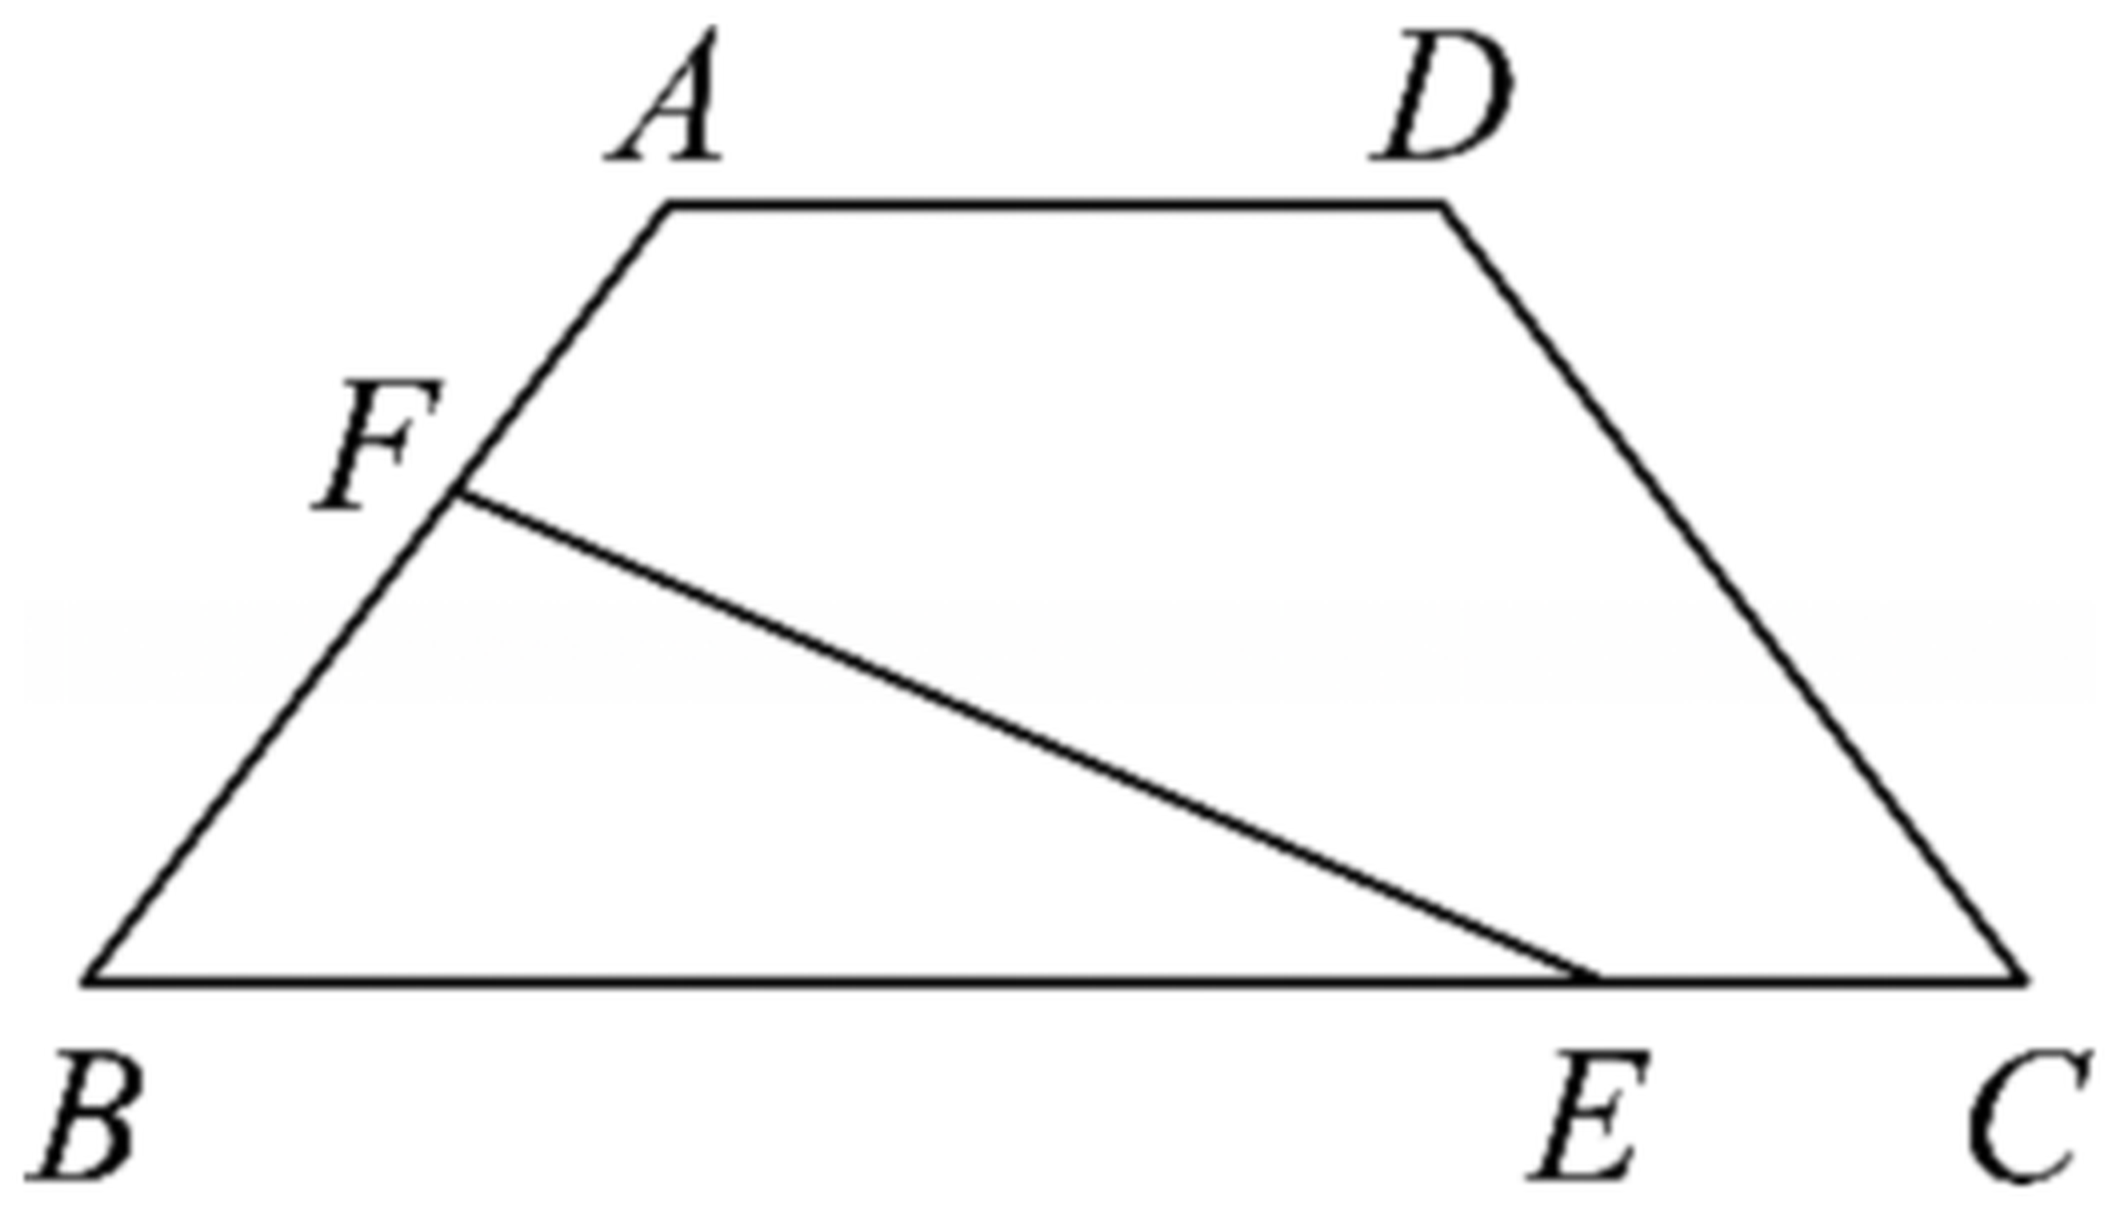
\includegraphics[width=0.46\textwidth]{figures/trapezoid_EF.png}
\end{center}

\begin{enumerate}[label=(\arabic*)]
\item 若 $EF$ 平分等腰梯形 $ABCD$ 的周长，设 $BE$ 长为 $x$，试用含 $x$ 的代数式表示
$\triangle BEF$ 的面积；
\item 是否存在线段 $EF$ 将等腰梯形 $ABCD$ 的周长和面积同时平分？若存在，求出此时 $BE$
的长；若不存在，请说明理由；
\item 是否存在线段 $EF$ 将等腰梯形 $ABCD$ 的周长和面积同时分成 $1:2$ 的两部分？
若存在，求此时 $BE$ 的长；若不存在，请说明理由.
\end{enumerate}

\ifanswer
\solbegin
\stepm{(1)}{过 $A$ 作 $AK\perp BC$ 交 $BC$ 于点 $K$，过 $F$ 作 $FG\perp BC$ 交 $BC$ 于点
$G$，}

\begin{center}
% 图取原卷截图、4× LANCZOS 放大（同梯形，多出虚线 $FG\perp BC$ 与 $AK\perp BC$
% 及两处直角符号；图只在【解析】里出现，故放进 \ifanswer 块）。
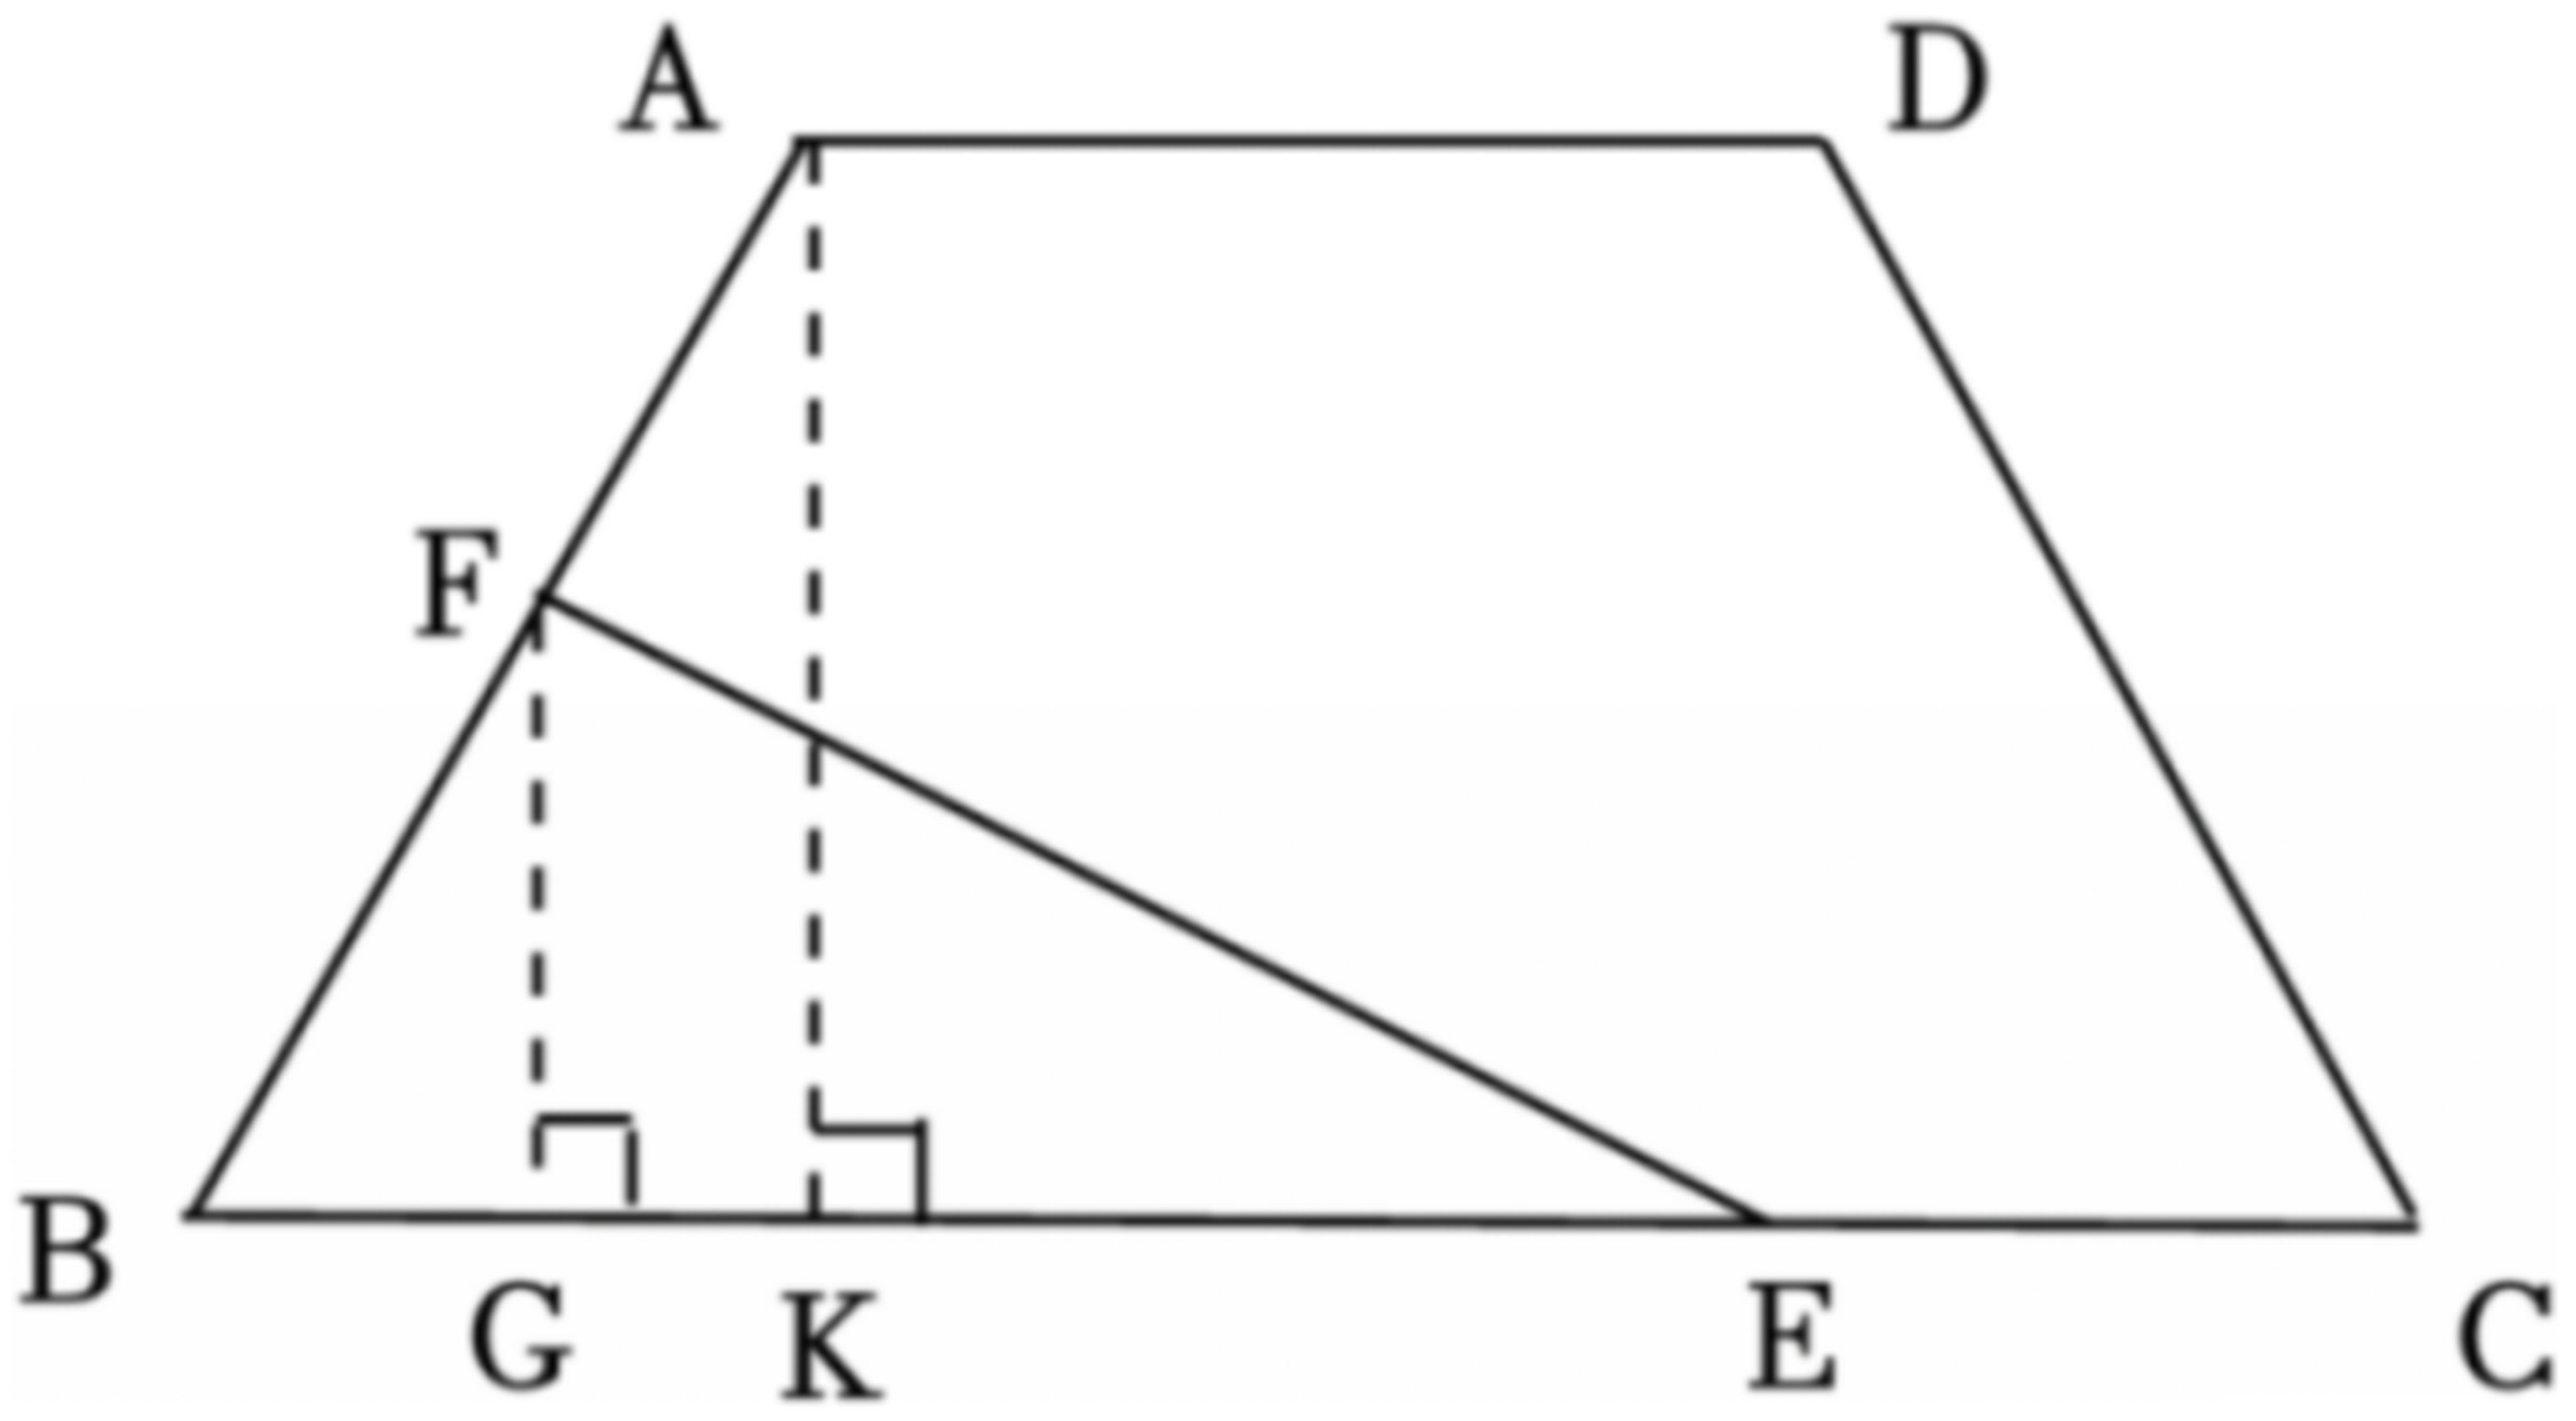
\includegraphics[width=0.62\textwidth]{figures/trapezoid_EF_aux.png}
\end{center}

\step{所以 $BK=\dfrac12\times(BC-AD)=\dfrac12\times(10-4)=3$，}
\step{$AK=\sqrt{AB^2-BK^2}=\sqrt{5^2-3^2}=4$，}
\step{由题意得，梯形 $ABCD$ 周长为 $24$，高为 $4$，面积为 $28$，}
\step{因为 $EF$ 平分等腰梯形 $ABCD$ 的周长，设 $BE$ 长为 $x$，则 $BF=12-x$，}
\step{由 $\begin{cases}0\leqslant12-x\leqslant5\\ 0\leqslant x\leqslant10\end{cases}$，
解得 $7\leqslant x\leqslant10$，}
\step{由题意得 $\triangle BFG\backsim\triangle BAK$，所以 $\dfrac{FG}{AK}=\dfrac{BF}{BA}$，
即 $\dfrac{FG}4=\dfrac{12-x}5$，}
\step{解得 $FG=\dfrac45(12-x)$，}
\step{所以 $S_{\triangle BEF}=\dfrac12BE\cdot FG
=-\dfrac25x^2+\dfrac{24}5x$（$7\leqslant x\leqslant10$）；}
\stepm{(2)}{存在，由 (1) 得 $-\dfrac25x^2+\dfrac{24}5x=\dfrac{28}2$，$x\in[7,10]$，}
\step{即 $x^2-12x+35=0$，解得 $x=7$ 或 $x=5$（舍去），}
\step{所以存在线段 $EF$ 将等腰梯形 $ABCD$ 的周长和面积同时平分，此时 $BE=7$；}
\stepm{(3)}{不存在，}
\step{情况一：$\triangle BEF$ 的面积$:$多边形 $AFECD$ 的面积 $=1:2$，
$(BE+BF):(AF+AD+DC+CE)=1:2$，}
\step{梯形周长的 $\dfrac13$ 是 $\dfrac{24}3=8$，面积的 $\dfrac13$ 是 $\dfrac{28}3$，}
\step{又因为 $BE=x$，所以 $BF=8-x$，}
\step{又因为 $\dfrac{FG}{AK}=\dfrac{BF}{BA}$，即 $\dfrac{FG}4=\dfrac{8-x}5$，
所以 $FG=\dfrac{32-4x}5$，}
\step{所以 $S_{\triangle BEF}=\dfrac12BE\times FG=-\dfrac25x^2+\dfrac{16}5x$，
所以 $\dfrac{28}3=-\dfrac25x^2+\dfrac{16}5x$，}
\step{整理得 $-3x^2+24x-70=0$，此时 $\Delta<0$，无解，故不存在；}
\step{情况二：$\triangle BEF$ 的面积$:$多边形 $AFECD$ 的面积 $=2:1$，
$(BE+BF):(AF+AD+DC+CE)=2:1$，}
\step{梯形周长的 $\dfrac13$ 为 $\dfrac{24}3=8$，面积的 $\dfrac13$ 为 $\dfrac{28}3$，
又 $BE=x$，所以 $BF=16-x$，}
\step{又 $\dfrac{FG}{AK}=\dfrac{BF}{BA}$，即 $\dfrac{FG}4=\dfrac{16-x}5$，
所以 $FG=\dfrac{64-4x}5$，}
\step{所以 $S_{\triangle BEF}=\dfrac12BE\times FG=-\dfrac25x^2+\dfrac{32}5x$，}
\step{所以 $\dfrac{28}3\times2=-\dfrac25x^2+\dfrac{32}5x$，
整理得 $-3x^2+48x-140=0$，}
\step{解得 $x=\dfrac{48+\sqrt{624}}6>10$，$x=\dfrac{48-\sqrt{624}}6<7$，
不符合题意，舍去，故不存在；}
\step{综上所述，不存在线段 $EF$ 将等腰梯形 $ABCD$ 的周长和面积同时分成 $1:2$ 的两部分.}
\solend

\fi

\ansspace[8]

\item 对集合 $\{1,2,\cdots,n\}$ 及其每一个非空子集 $A$，定义一个唯一确定的“交替和”
如下：将 $A$ 中的元素按照递减的次序排列，然后将第一个元素交替地减或加后继的元素所得的
结果，例如，子集 $\{1,2,4,6,9\}$ 的“交替和”是 $9-6+4-2+1=6$，子集 $\{5,6\}$ 的
“交替和”是 $6-5=1$，子集 $\{2\}$ 的交替和是 $2$；定义一个唯一确定的“交替积”如下：
将 $A$ 中的元素按照递减的次序排列，然后将第一个元素交替地除以或乘以后继的数所得的结果，
例如，集合 $\{1,2,4,6,9\}$ 的“交替积”是 $9\div6\times4\div2\times1=3$，
$\{5,6\}$ 的“交替积”是 $6\div5=1.2$，$\{2\}$ 的“交替积”是 $2$.

\begin{enumerate}[label=(\arabic*)]
\item 对于 $\{1,2,3,4,5,6,7,8,9\}$，求其所有子集的“交替和”的总和；
\item 对于 $\{1,2,\cdots,n\}$，求其所有子集的“交替和”的总和；
\item 对于 $\left\{n\mid\dfrac{495}{n+2}\in\N,n\in\Z\right\}$ 求其所有子集的
“交替积”的总和.
\end{enumerate}

\ifanswer
\solbegin
\stepm{(1)}{集合 $\{1,2,3,4,5,6,7,8,9\}$ 的子集中，除去 $\{9\}$ 外还有 $2^9-2$ 个
非空子集，}
\step{把这 $2^9-2$ 个非空子集两两组合后分别计算每一组中“交替和”之和，}
\step{组合原则是设 $A_i=\{9,a_1,a_2,\cdots\}$，$A_i^1=\{a_1,a_2,\cdots\}$，}
\step{集合 $A_i^1$ 的元素为集合 $A_i$ 中去掉 $9$ 的所有元素，把 $A_i$ 和 $A_i^1$
结合为一组，}
\step{显然，每组的“交替和”的和为 $9$，共有 $\dfrac{2^9-2}2$ 组，}
\step{所以，所有“交替和”之和应该为 $\dfrac{9(2^9-2)}2+9=2304$；}
\stepm{(2)}{集合 $\{1,2,\cdots,n\}$ 的子集中，除去 $\{n\}$ 外还有 $2^n-2$ 个非空子集，}
\step{把这 $2^n-2$ 个非空子集两两组合后分别计算每一组中“交替和”之和，}
\step{组合原则是设 $A_i=\{n,a_1,a_2,\cdots\}$，$A_i^1=\{a_1,a_2,\cdots\}$，}
\step{集合 $A_i^1$ 的元素为集合 $A_i$ 中去掉 $n$ 的所有元素，把 $A_i$ 和 $A_i^1$
结合为一组，}
\step{显然，每组的“交替和”的和为 $n$，共有 $\dfrac{2^n-2}2$ 组，}
% 注：下一行分子原卷印作花括号（其余同类处皆用圆括号），照抄未改，见文件头“原卷存疑”③。
\step{所以，所有“交替和”之和应该为 $\dfrac{n\{2^n-2\}}2+n=n\cdot2^{n-1}$；}
\stepm{(3)}{集合 $\left\{n\mid\dfrac{495}{n+2}\in\N,n\in\Z\right\}
=\{493,163,97,53,43,31,13,9,7,3,1,-1\}$，}
\step{其中除去 $\{-1\}$ 外还有 $2^{12}-2$ 个非空子集，}
% 注：下一行原卷把“把这”重复印了一次（“把这把这”），照抄未改，见文件头“原卷存疑”②。
\step{把这把这 $2^{12}-2$ 个非空子集两两组合后分别计算每一组中“交替积”之和，}
\step{组合原则是设 $A_j=\{-1,a_1,a_2,\cdots\}$，$A_j^1=\{a_1,a_2,\cdots\}$，}
\step{集合 $A_j^1$ 的元素为集合 $A_j$ 中去掉 $-1$ 的所有元素，把 $A_j$ 和 $A_j^1$
结合为一组，}
\step{显然，每组的“交替积”的和为 $0$，共有 $\dfrac{2^{12}-2}2$ 组，}
\step{所以，所有“交替积”之和应该为 $\dfrac{2^{12}-2}2\times0-1=-1$.}
\solend

\fi

\ansspace*[10]

\end{enumerate}

\end{document}
"
%
% 原始材料是微信公众号图文（公众号“魔都数学加油站”连载“27学年高一 30”，2026-09-23 发布，
% 原文标题“27学年高一30——2026-2027年上海市南洋模范中学高一上开学考”），
% 正文为 11 张 PNG 页。**同一篇里各页分辨率不一致**——第 2、3、9、10 页 4762×6735，
% 其余七页 2560×3620（已逐页打开确认，非下载缺档），取的是 mmbiz.qpic.cn/<hash>/0 的原图档。
% 原文本身就是一份**讲评版**：填空第 3—7 题下方印【答案】，第 8—12 题与其后各题印【解析】。
% 试题文字、答案与解析均照原卷录入，未改内容。卷面的粉色斜水印属水印，未录入。
%
% 卷首标题：原卷印作“2026-2027 年南洋模范中学高一上开学考”（公众号标题里的“上海市”
% 三字卷面标题行没有，本稿照卷面），年份区间按全稿惯例排 en dash，前缀照原卷保留“年”。
%
% 与原卷的排版差异（均已在 README“说明”中交代）：
%   ① 原文自**第 3 题**起（第 1、2 题未在该文中发布），故本稿题号亦自 3 起；
%   ② 原卷本就印有“一、填空题”“二、选择题”“三、解答题”三节标题，本稿照原卷分节，
%      只把标题改排成全稿统一的“大节标题”样式；
%   ③ 原卷填空第 3—7 题只印【答案】行、第 8 题起印【解析】（选择题答案写在解析末句
%      “故选 D／B”里），本稿统一改为试卷版隐去、答案版以 \ans{}／\ifanswer 块给出，
%      两版彻底分离；
%   ④ 子集符号原卷两种并用：第 7 题题干两处、第 19(2) 题作带下划线的 $\subseteq$，
%      第 17(2) 题解析作真包含的 $\subset$，本稿分别照录为 $\sub$ 与 $\subset$；
%   ⑤ 补集符号原卷一律作**上横线**（$\overline{A}$、$\overline{B}$），本稿照录；
%   ⑥ 原卷的实数集 R 一律作斜体（第 4 题、第 17 题与第 19 题题干的 $U=R$），
%      第 21(3) 题的自然数集与整数集作**粗体** $\mathbf{N}$、$\mathbf{Z}$，
%      本稿按全稿惯例统一写作 $\R$、$\N$、$\Z$；
%   ⑦ 原卷填空的横线约两个字宽，本稿按全稿惯例统一排 \blankline[4.4em]；
%   ⑧ 原卷未印副标题，本稿按全稿惯例补出副标题“集合与常用逻辑用语”——但本卷是开学考，
%      范围不止这一章：第 18 题是速度—时间图象题、第 20 题是等腰梯形的周长/面积平分问题，
%      副标题只标了主章节（见文末“高一30 专记”）；
%   ⑨ 第 13、14、18、20 题的图印在题干右侧、第 16 题的三幅图印在【解析】里的下一页顶部、
%      第 20 题【解析】另有一张带辅助线的图，本稿一律移至题干或解析之后；
%      图取原卷截图、4× LANCZOS 放大（见各 \includegraphics 前的注释）。
%
% 原卷存疑三处（均照抄原卷、未改，见源码中该处上方注释）：
%   ① 第 10 题【解析】验证“破晓集”时写的是 $\notin A$、$\in A$（如“$-2-2=-4\notin A$”），
%      但该处讨论的集合原题设里叫 $P$，同题②的“$x+y=2(k_1+k_2)\in A$”亦然——
%      本稿照抄未改（按文意应为 $P$）；
%   ② 第 21 题【解析】(3) 有“把这把这 $2^{12}-2$ 个非空子集”（“把这”重复印了一次）；
%   ③ 同题 (2) 的结论式分子原卷印作花括号 $\dfrac{n\{2^n-2\}}{2}$（其余同类处皆用圆括号）。

\documentclass[a4paper,11pt]{article}
\usepackage{common}

\begin{document}

\examtitlest[3]{2026--2027 年南洋模范中学高一上开学考}{集合与常用逻辑用语}

\bigsec{一、填空题}

\begin{enumerate}
\setcounter{enumi}{2}

\item 若集合 $A=\{x\mid x^2-2kx+7k=0\}$ 有且仅有三个真子集，则 $k$ 的取值范围是
\blankline[4.4em].

\ans{$(-\infty,0)\cup(7,+\infty)$}

\item “存在 $x\in\R$，使得 $x^2+2x+5=0$”的否定形式是 \blankline[4.4em].

\ans{对任何 $x\in\R$，都有 $x^2+2x+5\neq0$}

\item 下列命题中，$p$ 是 $q$ 的必要非充分条件的是 \blankline[4.4em].

① $p:x>2$ 且 $y>3$，$q:x+y>5$；

② $p$：四边形的四个角都相等，$q$：四边形是正方形.

\ans{②}

\item 若“条件 $\alpha:2\leqslant x\leqslant4$”是“条件 $\beta:3m-1\leqslant x\leqslant-m$”的
充分非必要条件，则 $m$ 的取值范围是 \blankline[4.4em].

\ans{$(-\infty,-4]$}

\item 满足 $\{1\}\sub M\sub\{1,2,4,5\}$ 的集合 $M$ 的个数为 \blankline[4.4em] 个.

\ans{$8$}

\item 已知集合 $A=\{1,2\}$，集合 $B=\{x\mid ax=6\}$，若 $A\cup B=A$，则 $a$ 的所有取值
构成的集合为 \blankline[4.4em].

\ifanswer
\solbegin
\step{因为 $A\cup B=A$，所以 $B\sub A$，}
\step{当 $a=0$ 时，$B=\varnothing$，满足 $B\sub A$；}
\step{当 $a\neq0$ 时，$B=\left\{\dfrac6a\right\}$，则 $\dfrac6a=1$ 或 $\dfrac6a=2$，
解得 $a=6$ 或 $a=3$，}
\step{综上所述，$a$ 的所有取值构成的集合为 $\{0,3,6\}$.}
\solend

\fi

\item 对于集合 $M$、$N$，定义 $M-N=\{x\mid x\in M\text{ 且 }x\notin N\}$，
$M\oplus N=(M-N)\cup(N-M)$，设 $A=\{y\mid y=|x|,x\in\R\}$，
$B=\{y\mid y=-(x-1)^2+2,x\in\R\}$，则 $A\oplus B=$ \blankline[4.4em].

\ifanswer
\solbegin
\step{由已知 $A=[0,+\infty)$，$B=(-\infty,2]$，}
\step{由于 $A-B=(2,+\infty)$，$B-A=(-\infty,0)$，}
\step{故 $A\oplus B=(A-B)\cup(B-A)=(-\infty,0)\cup(2,+\infty)$.}
\solend

\fi

\item 设 $P$ 为非空实数集满足：对任意给定的 $x$、$y\in P$（$x$、$y$ 可以相同），都有
$x+y\in P$，$x-y\in P$，$xy\in P$，则称 $P$ 为破晓集. 关于破晓集有下列结论：
①集合 $P=\{-2,-1,0,1,2\}$ 为破晓集；②集合 $P=\{x\mid x=2n,n\in\Z\}$ 为破晓集；
③若集合 $P_1$、$P_2$ 为破晓集，则 $P_1\cup P_2$ 为破晓集；④若集合 $P$ 为破晓集，
则一定有 $0\in P$；⑤若集合 $P_1$、$P_2$ 为破晓集，则 $P_1\cap P_2$ 为破晓集；
其中正确结论的序号是 \blankline[4.4em].

\ifanswer
\solbegin
% 注：以下几步原卷把该集合记作 $A$（题设里叫 $P$），照抄未改，见文件头“原卷存疑”①。
\step{对于①：$-2-2=-4\notin A$，故集合 $P=\{-2,-1,0,1,2\}$ 不为破晓集，故①错误；}
\step{②设 $x$、$y\in A$，则 $x=2k_1$，$y=2k_2$，且 $k_1$、$k_2\in\Z$，}
\step{故 $x+y=2(k_1+k_2)\in A$，$x-y=2(k_1-k_2)\in A$，$xy=4k_1k_2\in A$，}
\step{故集合 $P=\{x\mid x=2n,n\in\Z\}$ 为破晓集，故②正确；}
\step{③若集合 $P_1$、$P_2$ 为破晓集，设 $P_1=\{x\mid x=2k,k\in\Z\}$，
$P_2=\{x\mid x=3k,k\in\Z\}$，}
\step{但是 $P_1\cup P_2$ 不为破晓集，如 $x=2$，$y=3$ 时，$x+y=5$，
故 $5\notin(P_1\cup P_2)$，故③错误；}
\step{④若集合 $P$ 为破晓集，则取 $x=y$，$x-y=0\in A$，则一定有 $0\in P$，故④正确.}
\step{⑤正确；}
\step{故正确的是②④⑤.}
\solend

\fi

\item 已知集合 $M$ 的元素均为正整数，定义集合 $M$ 的“变项和”为：将 $M$ 中每个元素 $m$
都乘以 $(-1)^m$ 后再求和. 若集合 $A=\{n\mid1\leqslant n\leqslant10,n\in\N\}$，则集合 $A$
的所有非空子集的“变项和”的总和为 \blankline[4.4em].

\ifanswer
\solbegin
\step{$A$ 集合的所有非空子集中，每个元素出现的次数都是
$(2^{10}-1)-(2^9-1)=2^9$，}
\step{则集合 $A$ 的所有非空子集的“变项和”的总和为
$1\times(-1)^1\times2^9+2\times(-1)^2\times2^9+\cdots+10\times(-1)^{10}\times2^9$}
\step{$=(-1+2-3+4-\cdots-9+10)\times2^9=5\times2^9=2560$.}
\solend

\fi

\item 已知集合 $A=[t,t+1]\cup[t+4,t+9]$，$0\notin A$，存在正数 $\lambda$，使得对任意
$a\in A$，都有 $\dfrac\lambda a\in A$，则 $t$ 的值是 \blankline[4.4em].

\ifanswer
\solbegin
\step{当 $t>0$ 时，当 $a\in[t,t+1]$ 时，$\dfrac\lambda a\in[t+4,t+9]$，}
\step{当 $a\in[t+4,t+9]$ 时，$\dfrac\lambda a\in[t,t+1]$，}
\step{即当 $a=t$ 时，$\dfrac\lambda a\leqslant t+9$；当 $a=t+9$ 时，
$\dfrac\lambda a\geqslant t$，即 $\lambda=t(t+9)$；}
\step{当 $a=t+1$ 时，$\dfrac\lambda a\geqslant t+4$，当 $a=t+4$ 时，
$\dfrac\lambda a\leqslant t+1$，即 $\lambda=(t+1)(t+4)$，}
\step{所以 $t(t+9)=(t+1)(t+4)$，解得 $t=1$.}
\step{当 $t+1<0<t+4$ 时，当 $a\in[t,t+1]$ 时，$\dfrac\lambda a\in[t,t+1]$.}
\step{当 $a\in[t+4,t+9]$ 时，则 $\dfrac\lambda a\in[t+4,t+9]$，}
\step{即当 $a=t$ 时，$\dfrac\lambda a\leqslant t+1$，当 $a=t+1$ 时，
$\dfrac\lambda a\geqslant t$，即 $\lambda=t(t+1)$，}
\step{即当 $a=t+4$ 时，$\dfrac\lambda a\leqslant t+9$，当 $a=t+9$ 时，
$\dfrac\lambda a\geqslant t+4$，即 $\lambda=(t+4)(t+9)$，}
\step{所以 $t(t+1)=(t+4)(t+9)$，解得 $t=-3$.}
\step{当 $t+9<0$ 时，同理可得无解.}
\step{综上，$t$ 的值为 $1$ 或 $-3$.}
\solend

\fi

\end{enumerate}

\bigsec{二、选择题}

\begin{enumerate}
\setcounter{enumi}{12}

% 这道题是“题干 + 图 + 选项”约 6cm 的一整块，页末放不下就会被拆开（切页审计的 A 类），
% 故在题前先量一次页高：不够就把整道题干连图带选项一起挪到次页。
\needvspace{6.5cm}
\item 设 $U=\{1,2,3,4,5\}$，$A$、$B$ 都是 $U$ 的子集，且 $A\cap B=\{5\}$，
$\overline{A}\cap B=\{4\}$，$\overline{A}\cap\overline{B}=\{1,2\}$，
则以下四个判断中正确的是\mbox{（\quad）}

\begin{center}
% 图取原卷截图、4× LANCZOS 放大（原卷把图印在题干右侧，本稿移至此处，见文件头⑨）。
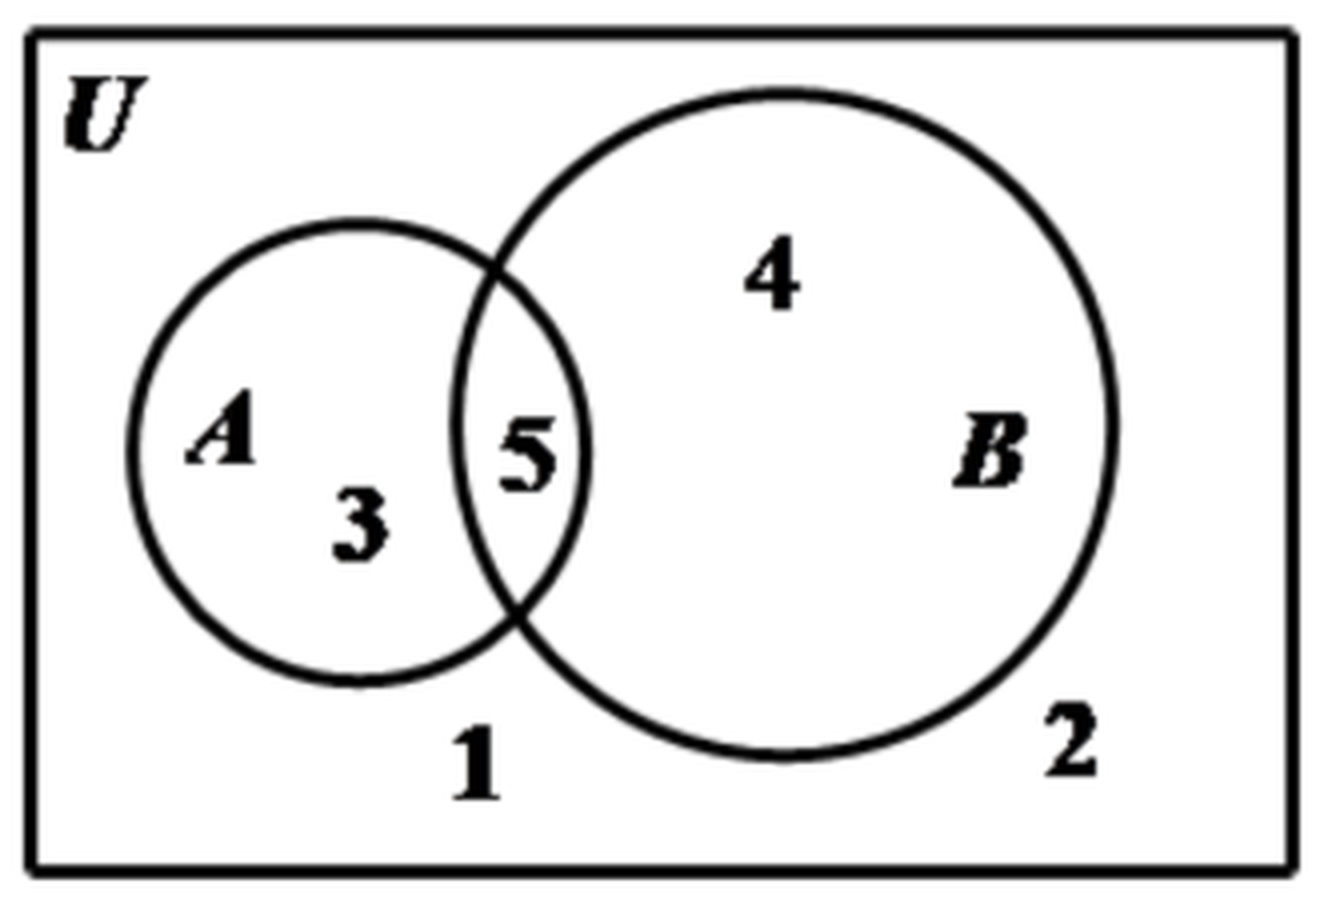
\includegraphics[width=0.28\textwidth]{figures/venn_U5_AB.png}
\end{center}

\keepwithprev
A. $3\notin A$ 且 $3\notin B$\qquad\qquad B. $3\in A$ 且 $3\in B$

C. $3\notin A$ 且 $3\in B$\qquad\qquad D. $3\in A$ 且 $3\notin B$

\ans{$D$}

\ifanswer
\solbegin
\step{画出韦恩图，得 $A=\{5,3\}$，$B=\{5,4\}$，}
\step{则 $3\in A$ 且 $3\notin B$. 故选 $D$.}
\solend

\fi

% 同第 13 题：整块（题干 + 图 + 选项）在答案版还要再挂【答案】【解析】，页末更易被拆开。
\needvspace{7.5cm}
\item 如图表示图形阴影部分的是\mbox{（\quad）}

\begin{center}
% 图取原卷截图、4× LANCZOS 放大（三圆 $A$、$B$、$C$，阴影为整个 $A$ 圆加 $B\cap C$）。
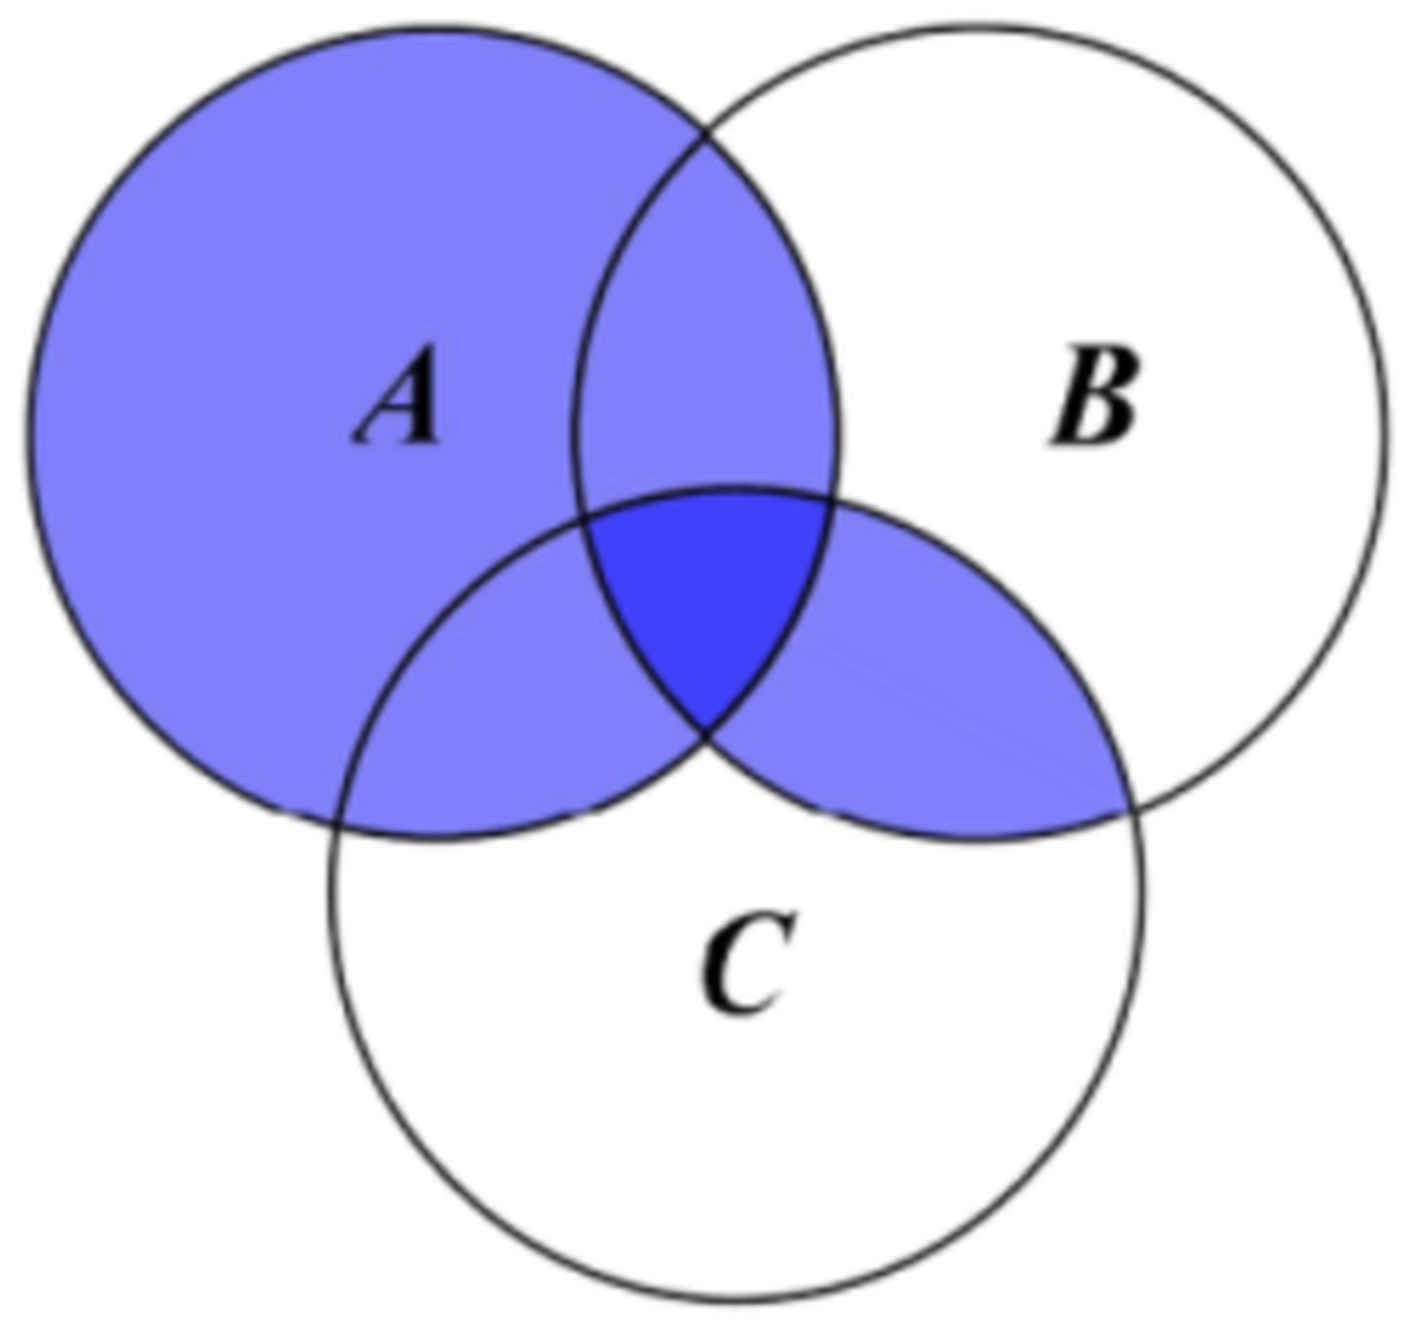
\includegraphics[width=0.30\textwidth]{figures/venn_A_union_BC.png}
\end{center}

\keepwithprev
A. $(A\cup C)\cap(B\cup C)$\qquad\qquad B. $(A\cup B)\cap(A\cup C)$

C. $(A\cup B)\cap(B\cup C)$\qquad\qquad D. $(A\cup B)\cap C$

\ans{$B$}

\ifanswer
\solbegin
\step{图中阴影部分表示元素满足是 $A$ 中的元素，或者是 $B$ 与 $C$ 的公共元素，}
\step{故可以表示为 $A\cup(B\cap C)$，也可以表示为 $(A\cup B)\cap(A\cup C)$.
故选 $B$.}
\solend

\fi

\item 设集合 $M=\left\{x\mid m\leqslant x\leqslant m+\dfrac34\right\}$，
$N=\left\{x\mid n-\dfrac13\leqslant x\leqslant n\right\}$，且 $M$、$N$ 都是集合
$\{x\mid0\leqslant x\leqslant1\}$ 的子集，如果把 $b-a$ 叫做集合
$\{x\mid a\leqslant x\leqslant b\}$ 的“长度”，那么集合 $M\cap N$ 的“长度”的
最小值是\mbox{（\quad）}

\keepwithprev
A. $\dfrac23$\qquad B. $\dfrac1{12}$\qquad C. $\dfrac13$\qquad D. $\dfrac5{12}$

\ans{$B$}

\ifanswer
\solbegin
\step{$M$ 的长度为 $\dfrac34$，$N$ 的长度为 $\dfrac13$，}
\step{当集合 $M\cap N$ 的长度的最小值时，$M$ 与 $N$ 应分别在区间 $[0,1]$ 的左右两端，}
\step{故 $M\cap N$ 的长度的最小值是 $\dfrac34+\dfrac13-1=\dfrac1{12}$，故选 $B$.}
\solend

\fi

\item 定义集合运算 $A-B=\{x\mid x\in A\text{ 且 }x\notin B\}$ 称为集合 $A$ 与集合 $B$ 的
差集；定义集合运算 $A\Delta B=(A-B)\cup(B-A)$ 称为集合 $A$ 与集合 $B$ 的对称差，
有以下 $4$ 个等式：① $A\Delta B=B\Delta A$；② $(A\Delta B)\Delta C=A\Delta(B\Delta C)$；
③ $A\cap(B\Delta C)=(A\cap B)\Delta(A\cap C)$；
④ $A\cup(B\Delta C)=(A\cup B)\Delta(A\cup C)$，
则 $4$ 个等式中恒成立的是\mbox{（\quad）}

\keepwithprev
A. ①②\qquad B. ①②③\qquad C. ①②④\qquad D. ①②③④

\ans{$B$}

\ifanswer
\solbegin
\step{对于①，由 $B\Delta A=(B-A)\cup(A-B)=(A-B)\cup(B-A)=A\Delta B$，
所以①正确；}
\step{对于②，由 $A-B=\{x\mid x\in A\text{ 且 }x\notin B\}
=\{x\mid x\in A,x\notin(A\cap B)\}=A-(A\cap B)$，}
\step{同理可得 $B-A=B-(A\cap B)$，}
\step{则 $A\Delta B=(A-B)\cup(B-A)=(A\cup B)-(A\cap B)$，}
\step{所以 $(A\Delta B)\Delta C=(A\Delta B)\cup C-(A\Delta B)\cap C$，}
\step{所以表示的集合为图（1）中阴影部分所表示的集合，如图所示，}
\step{同理 $A\Delta(B\Delta C)=A\cup(B\Delta C)-A\cap(B\Delta C)$，
也表示图（1）中阴影部分所表示的集合，}
\step{所以 $(A\Delta B)\Delta C=A\Delta(B\Delta C)$，所以②正确；}

\begin{center}
% 图取原卷截图、4× LANCZOS 放大（原卷印在下一页顶部，共三幅三圆韦恩图：
% 图（1）一幅、图（2）左右两幅，图（2）两幅下方各有一行式子标注）。
% 图只在【解析】里出现，故放进 \ifanswer 块，试卷版不排。
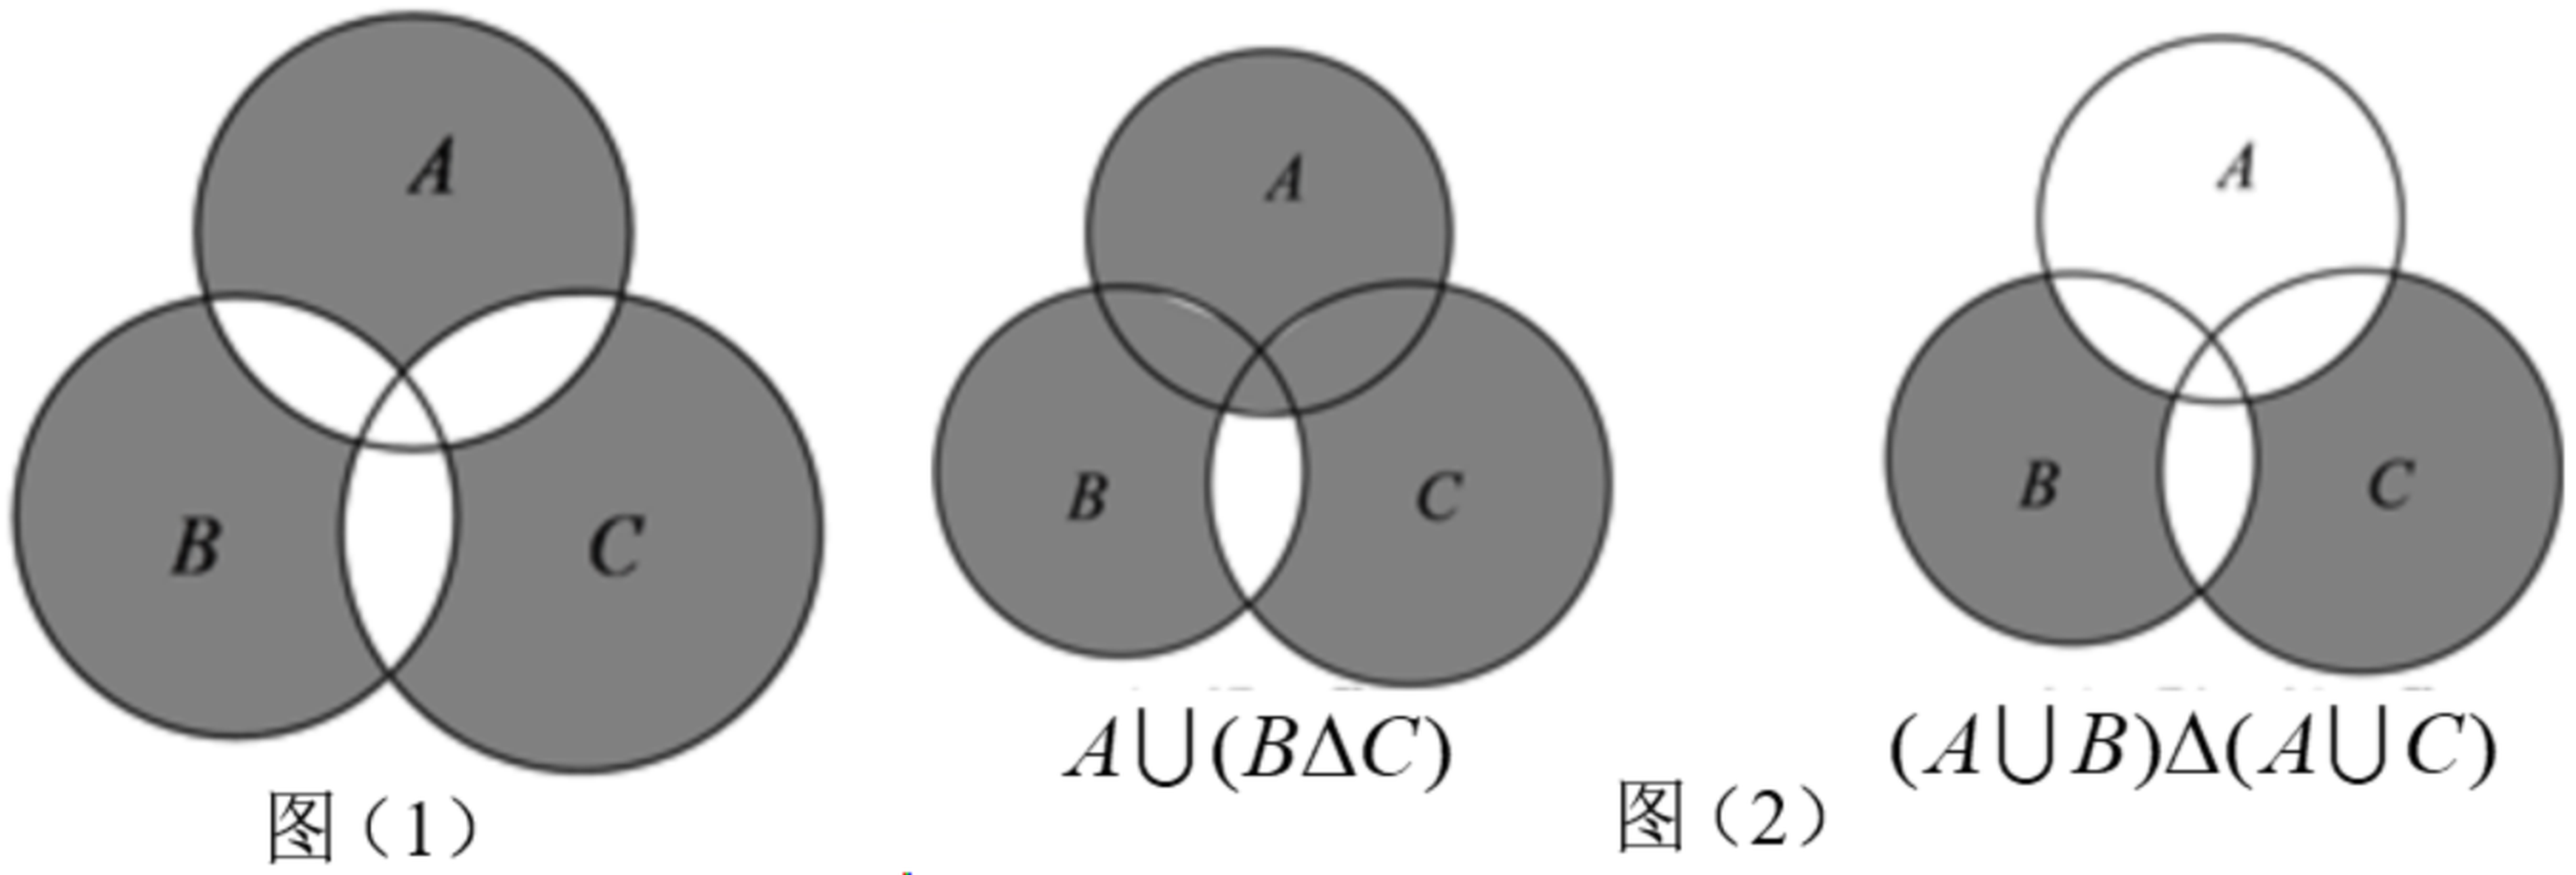
\includegraphics[width=0.86\textwidth]{figures/venn_symdiff3.png}
\end{center}

\step{对于③，由 $A\cap(B\Delta C)=A\cap(B\cup C-B\cap C)
=A\cap(B\cup C)-A\cap(B\cap C)$}
\step{$=(A\cap B)\cup(A\cap C)-(A\cap B)\cap(A\cap C)=(A\cap B)\Delta(A\cap C)$，
所以③正确；}
\step{对于④，如图（2）所示，$A\cup(B\Delta C)\neq(A\cup B)\Delta(A\cup C)$，
所以④错误.}
\step{故选 $B$.}
\solend

\fi

\end{enumerate}

\bigsec{三、解答题}

\begin{enumerate}
\setcounter{enumi}{16}

\item 已知集合 $M=\{x\mid a-1\leqslant x\leqslant2a+3\}$，$P=\{x\mid-2<x\leqslant4\}$，
全集 $U=\R$.

\begin{enumerate}[label=(\arabic*)]
\item 当 $a=2$ 时，求 $M\cap P$；
\item 若 $x\in P$ 是 $x\in M$ 的必要不充分条件，求实数 $a$ 的取值范围.
\end{enumerate}

\ifanswer
\solbegin
\stepm{(1)}{当 $a=2$ 时，集合 $M=\{x\mid1\leqslant x\leqslant7\}$，}
\step{所以 $M\cap P=\{x\mid1\leqslant x\leqslant4\}$；}
\stepm{(2)}{因为 $x\in P$ 是 $x\in M$ 的必要不充分条件，所以 $M\subset P$，}
\step{当 $M=\varnothing$ 时，$a-1>2a+3$，解得 $a<-4$，}
\step{当 $M\neq\varnothing$ 时，则
$\begin{cases}a-1\leqslant2a+3\\ a-1>-2\\ 2a+3\leqslant4\end{cases}$，
解得 $-1<a\leqslant\dfrac12$，}
\step{综上所述，实数 $a$ 的取值范围为
$(-\infty,-4)\cup\left(-1,\dfrac12\right]$.}
\solend

\fi

\ansspace[6]

\item 一辆汽车在某段路程中的行驶速度与时间的关系如图：

\begin{center}
% 图取原卷截图、4× LANCZOS 放大（速度—时间图：纵轴 $v/(\mathrm{km/h})$、
% 横轴 $t(\mathrm{h})$，$t\in[0,1]$、$[1,2]$、$[2,3]$ 三段矩形条高 50、80、90）。
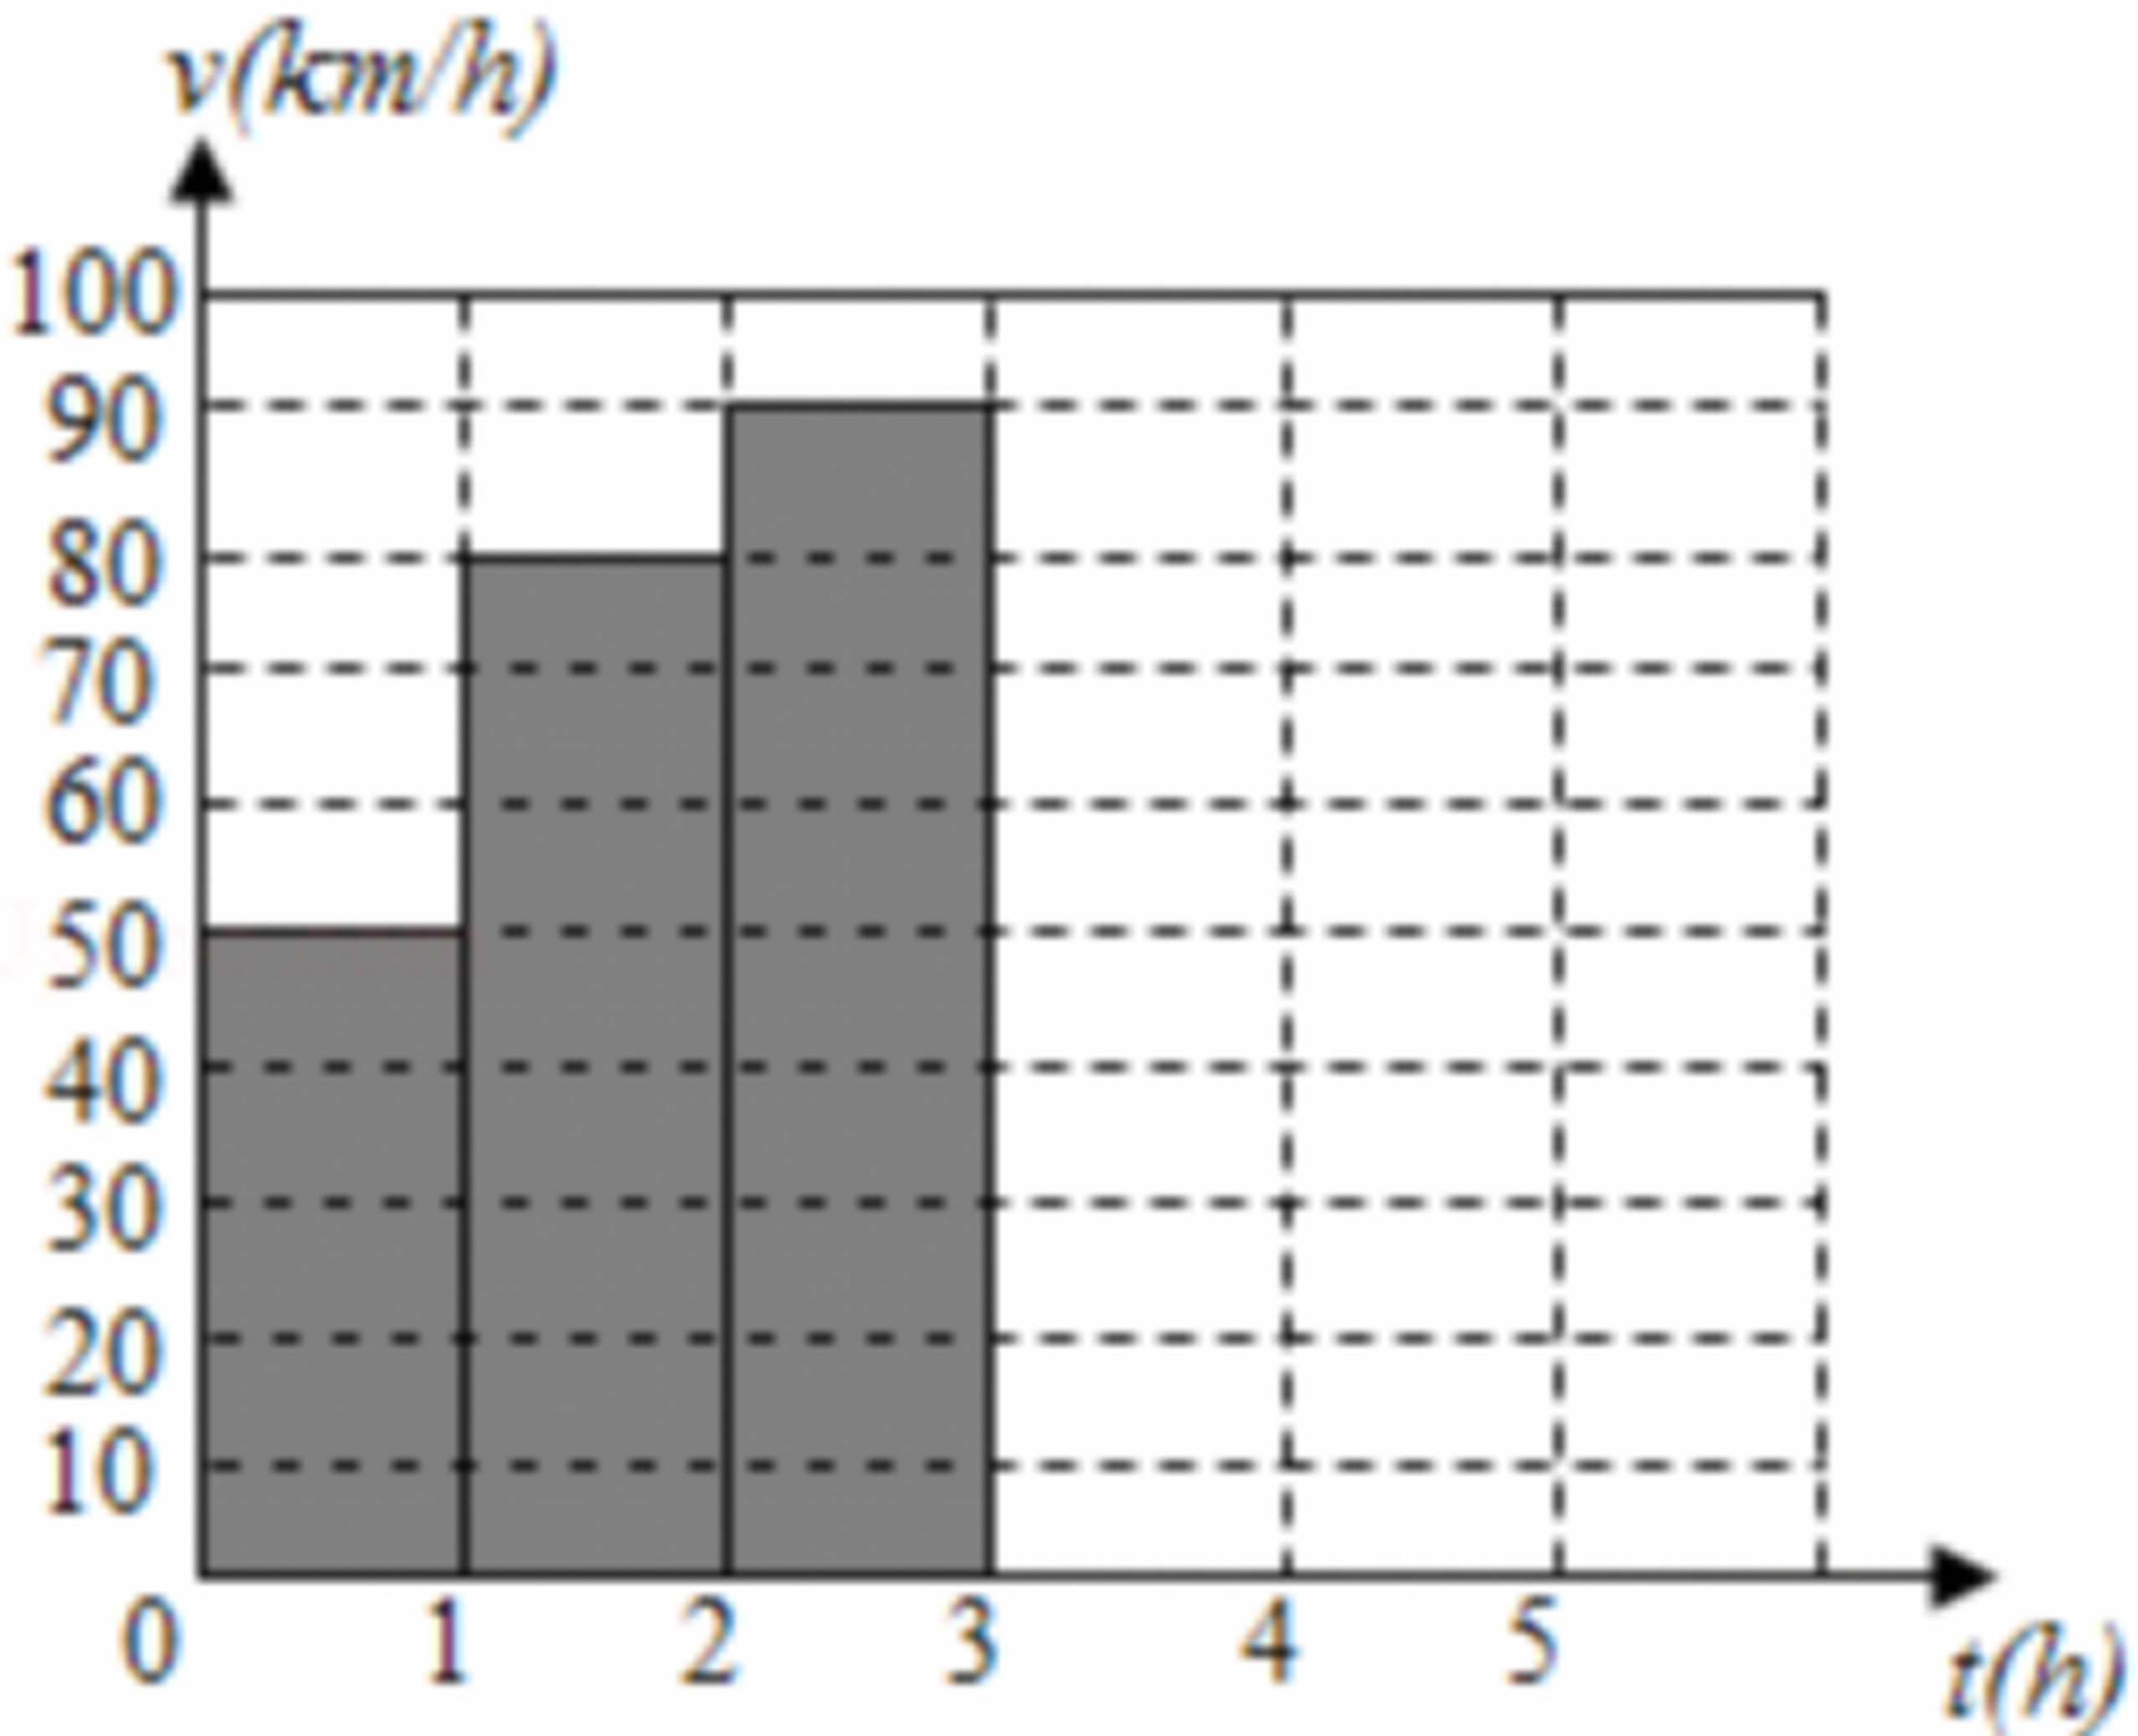
\includegraphics[width=0.52\textwidth]{figures/speed_time_bars.png}
\end{center}

\begin{enumerate}[label=(\arabic*)]
\item 求图中阴影部分的面积，并说明所求面积的实际意义；
\item 假设这辆汽车的里程表在汽车行驶这段路程前的读数为 $2004\,\mathrm{km}$，
试将汽车行驶这段路程时汽车里程表读数 $S$ 表示为时间 $t$ 的函数，
并求出当汽车里程表读数为 $2094\,\mathrm{km}$ 时，汽车行驶了多少时间？
\end{enumerate}

\ifanswer
\solbegin
\stepm{(1)}{由一辆汽车在某段路程中的行驶速度与时间的关系图，}
\step{得阴影部分的面积为 $50\times1+80\times1+90\times1=220$，}
\step{阴影部分的面积表示汽车在 $3$ 小时内行驶的路程为 $220\,\mathrm{km}$.}
\stepm{(2)}{$S=\begin{cases}
50t+2004,&0\leqslant t<1\\
80(t-1)+2054,&1\leqslant t<2\\
90(t-2)+2134,&2\leqslant t\leqslant3
\end{cases}$}
\step{令 $80(t-1)+2054=2094$，解得 $t=1.5$，所以汽车行驶 $1.5$ 小时.}
\solend

\fi

\ansspace[6]

\item 已知集合 $A=\{x\mid x<-2\text{ 或 }x\geqslant3\}$，$U=\R$.

\begin{enumerate}[label=(\arabic*)]
\item 求 $\overline{A}$；
\item 若 $B=\{x\mid mx-1>0\}$，当 $B\sub A$ 时，求实数 $m$ 的取值范围；
\item 若 $B=\{x\mid2m-6\leqslant x\leqslant m+4\}$，当 $B\cap\overline{A}=\varnothing$ 时，
求实数 $m$ 的取值范围.
\end{enumerate}

\ifanswer
\solbegin
\stepm{(1)}{因为集合 $A=\{x\mid x<-2\text{ 或 }x\geqslant3\}$，$U=\R$，
所以 $\overline{A}=\{x\mid-2\leqslant x<3\}$；}
\stepm{(2)}{当 $m=0$ 时，$B=\varnothing$，符合题意，}
\step{当 $m>0$ 时，$B=\left\{x\mid x>\dfrac1m\right\}$，则 $\dfrac1m\geqslant3$，
解得 $0<m\leqslant\dfrac13$，}
\step{当 $m<0$ 时，$B=\left\{x\mid x<\dfrac1m\right\}$，则 $\dfrac1m\leqslant-2$，
解得 $-\dfrac12\leqslant m<0$，}
\step{综上所述，实数 $m$ 的取值范围 $\left[-\dfrac12,\dfrac13\right]$；}
\stepm{(3)}{由题意得 $B=\{x\mid2m-6\leqslant x\leqslant m+4\}$，
$\overline{A}=\{x\mid-2\leqslant x<3\}$，且 $B\cap\overline{A}=\varnothing$，}
\step{当 $B=\varnothing$ 时，$2m-6>m+4$，解得 $m>10$，}
\step{当 $B\neq\varnothing$ 时，则 $\begin{cases}2m-6\leqslant m+4\\ m+4<-2\end{cases}$
或 $\begin{cases}2m-6\leqslant m+4\\ 2m-6\geqslant3\end{cases}$，}
\step{解得 $m<-6$ 或 $\dfrac92\leqslant m\leqslant10$，}
\step{综上所述，实数 $m$ 的取值范围为
$(-\infty,-6)\cup\left[\dfrac92,+\infty\right)$.}
\solend

\fi

\ansspace[8]

\item 在等腰梯形 $ABCD$ 中，$AB=DC=5$，$AD=4$，$BC=10$. 点 $E$ 在下底边 $BC$ 上.
点 $F$ 在腰 $AB$ 上.

\begin{center}
% 图取原卷截图、4× LANCZOS 放大（等腰梯形 $ABCD$ 与线段 $FE$，无辅助线）。
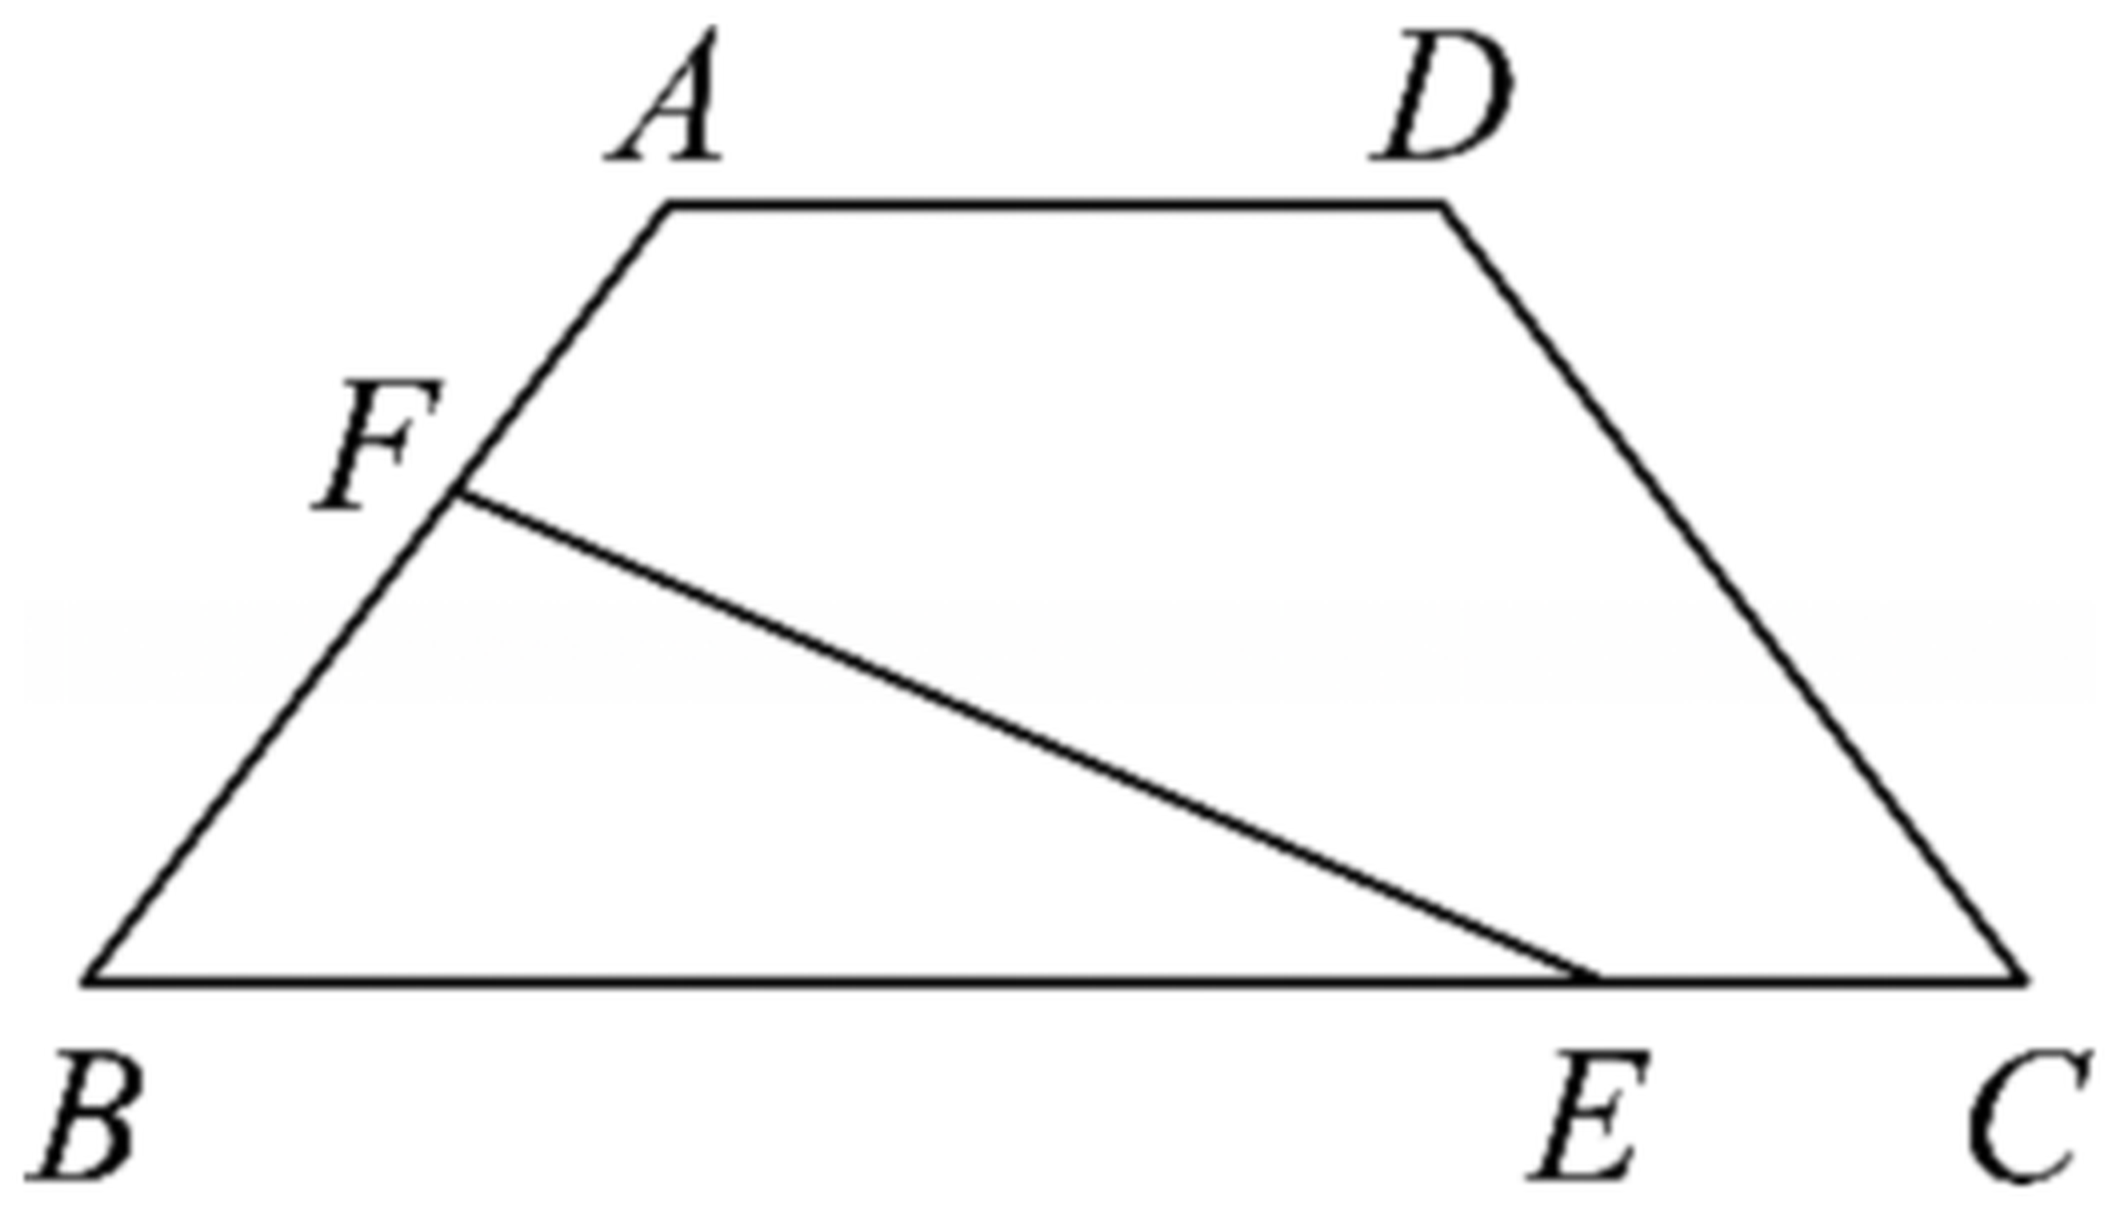
\includegraphics[width=0.46\textwidth]{figures/trapezoid_EF.png}
\end{center}

\begin{enumerate}[label=(\arabic*)]
\item 若 $EF$ 平分等腰梯形 $ABCD$ 的周长，设 $BE$ 长为 $x$，试用含 $x$ 的代数式表示
$\triangle BEF$ 的面积；
\item 是否存在线段 $EF$ 将等腰梯形 $ABCD$ 的周长和面积同时平分？若存在，求出此时 $BE$
的长；若不存在，请说明理由；
\item 是否存在线段 $EF$ 将等腰梯形 $ABCD$ 的周长和面积同时分成 $1:2$ 的两部分？
若存在，求此时 $BE$ 的长；若不存在，请说明理由.
\end{enumerate}

\ifanswer
\solbegin
\stepm{(1)}{过 $A$ 作 $AK\perp BC$ 交 $BC$ 于点 $K$，过 $F$ 作 $FG\perp BC$ 交 $BC$ 于点
$G$，}

\begin{center}
% 图取原卷截图、4× LANCZOS 放大（同梯形，多出虚线 $FG\perp BC$ 与 $AK\perp BC$
% 及两处直角符号；图只在【解析】里出现，故放进 \ifanswer 块）。
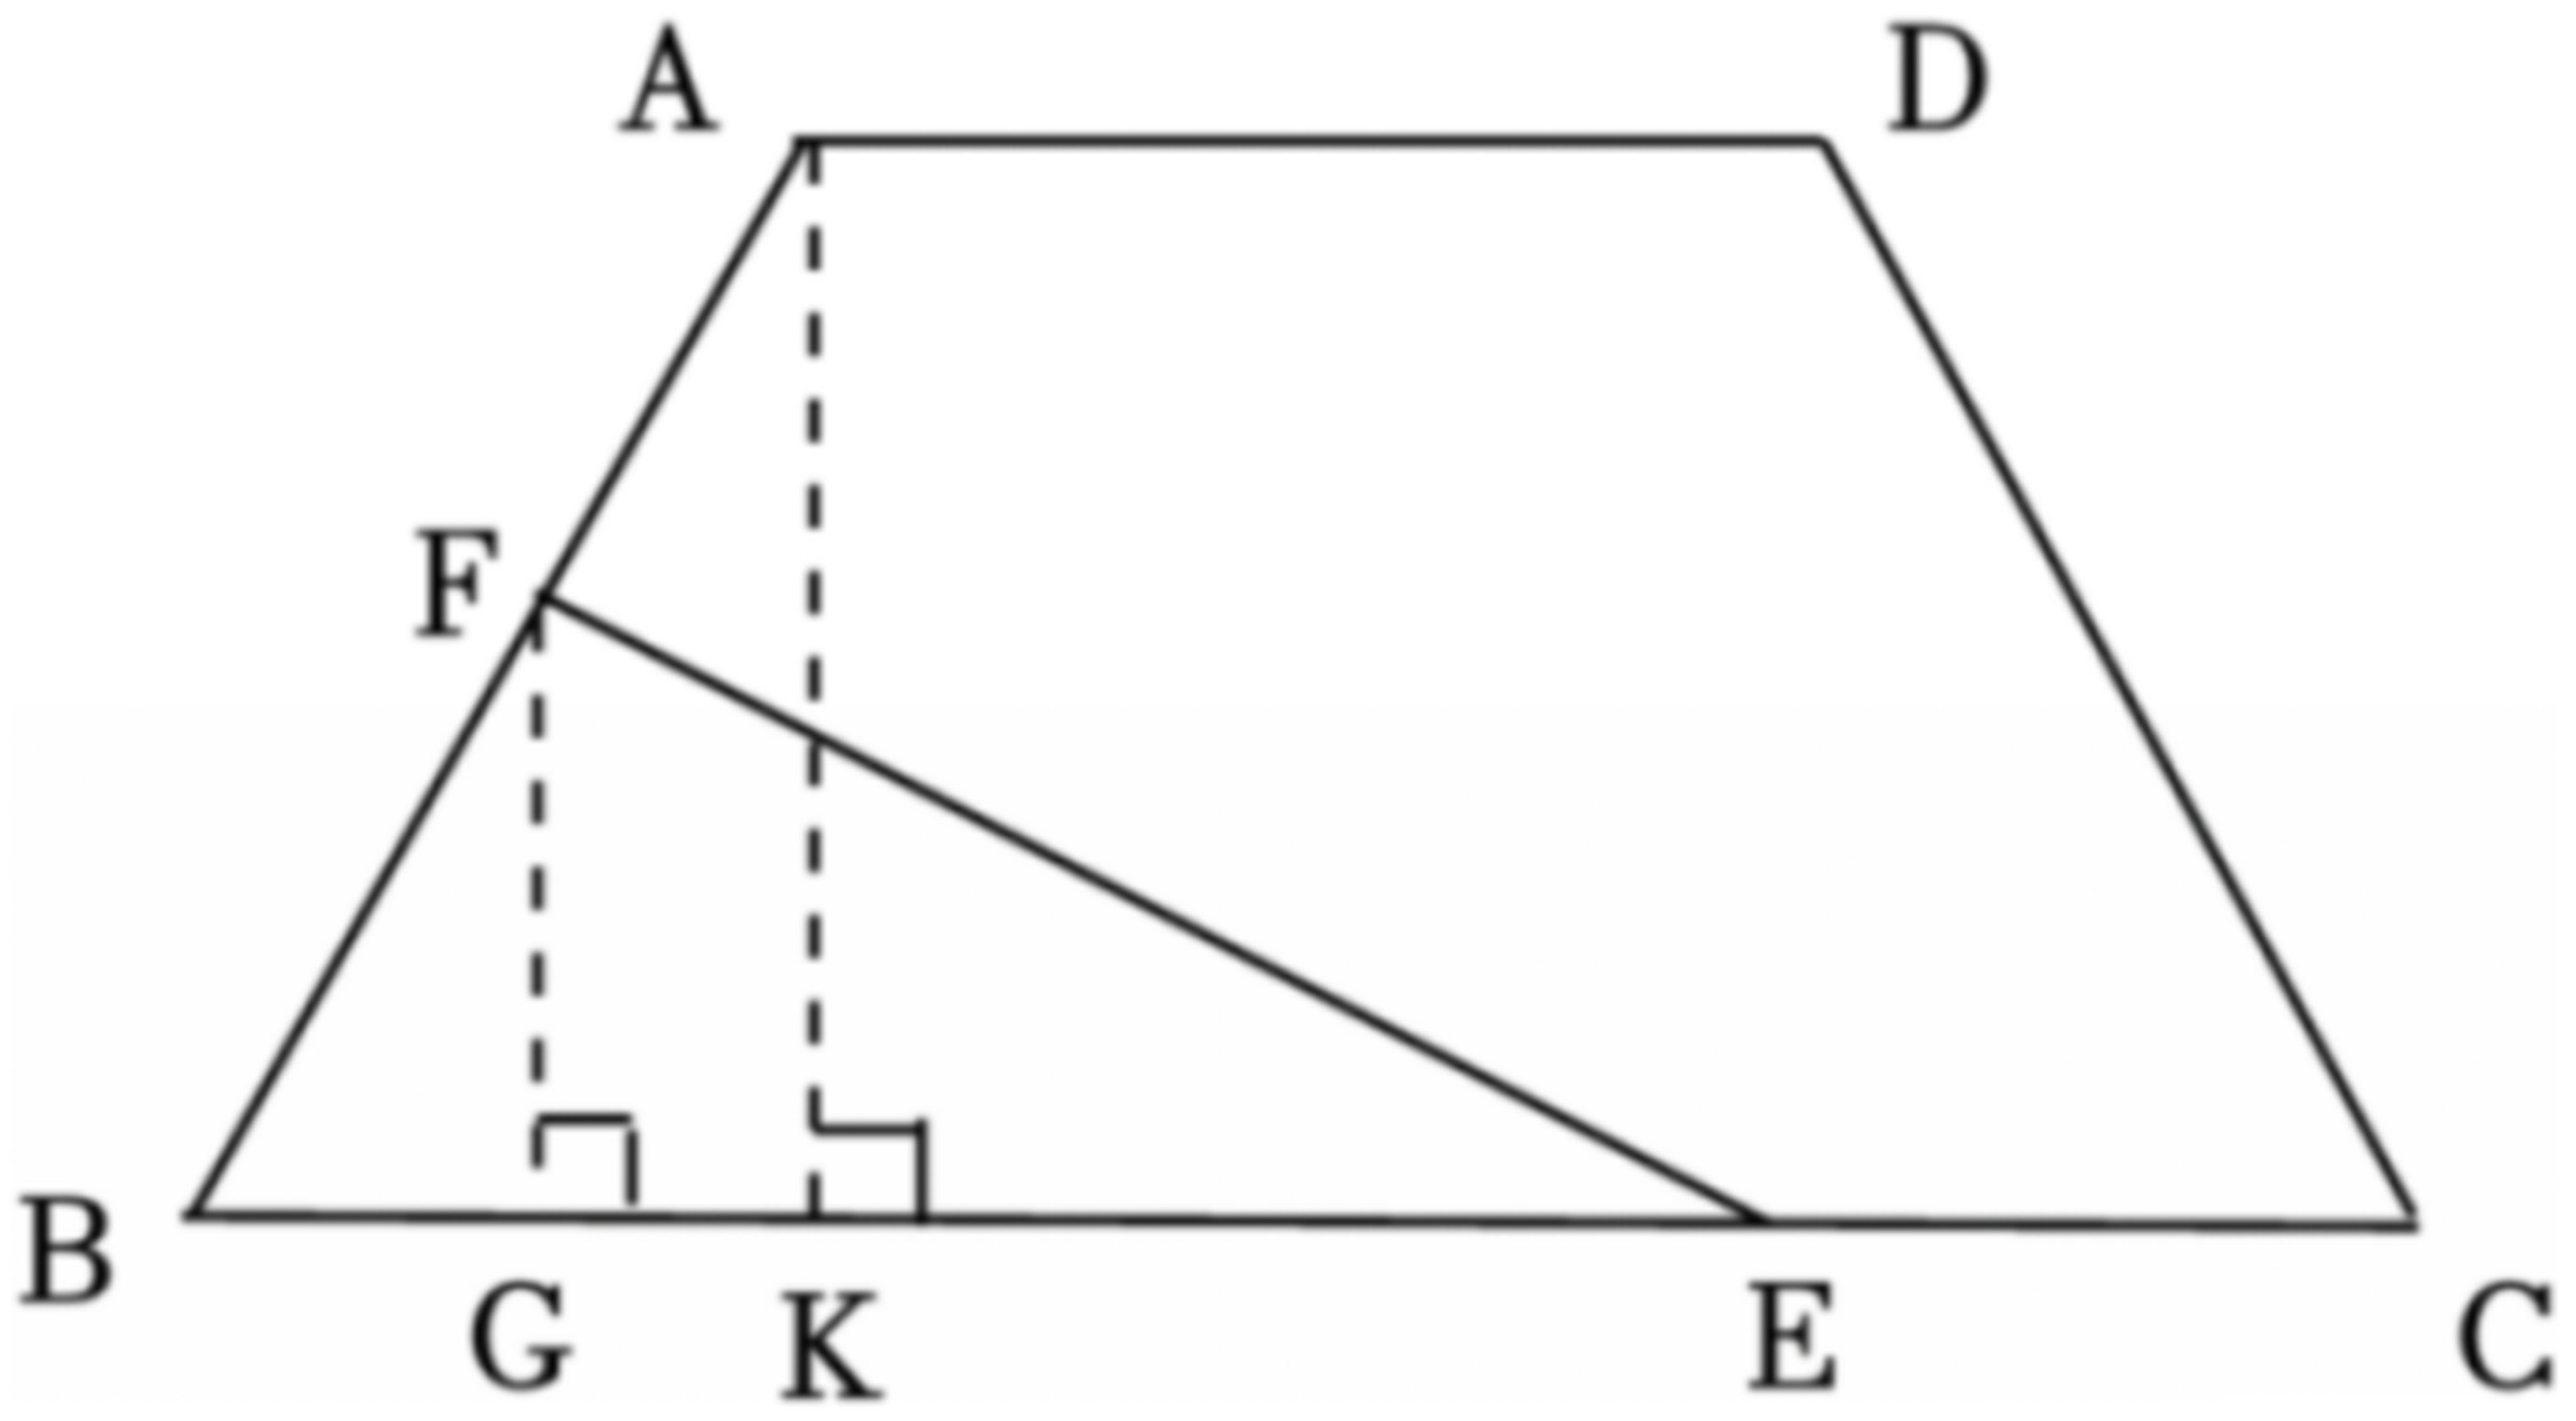
\includegraphics[width=0.62\textwidth]{figures/trapezoid_EF_aux.png}
\end{center}

\step{所以 $BK=\dfrac12\times(BC-AD)=\dfrac12\times(10-4)=3$，}
\step{$AK=\sqrt{AB^2-BK^2}=\sqrt{5^2-3^2}=4$，}
\step{由题意得，梯形 $ABCD$ 周长为 $24$，高为 $4$，面积为 $28$，}
\step{因为 $EF$ 平分等腰梯形 $ABCD$ 的周长，设 $BE$ 长为 $x$，则 $BF=12-x$，}
\step{由 $\begin{cases}0\leqslant12-x\leqslant5\\ 0\leqslant x\leqslant10\end{cases}$，
解得 $7\leqslant x\leqslant10$，}
\step{由题意得 $\triangle BFG\backsim\triangle BAK$，所以 $\dfrac{FG}{AK}=\dfrac{BF}{BA}$，
即 $\dfrac{FG}4=\dfrac{12-x}5$，}
\step{解得 $FG=\dfrac45(12-x)$，}
\step{所以 $S_{\triangle BEF}=\dfrac12BE\cdot FG
=-\dfrac25x^2+\dfrac{24}5x$（$7\leqslant x\leqslant10$）；}
\stepm{(2)}{存在，由 (1) 得 $-\dfrac25x^2+\dfrac{24}5x=\dfrac{28}2$，$x\in[7,10]$，}
\step{即 $x^2-12x+35=0$，解得 $x=7$ 或 $x=5$（舍去），}
\step{所以存在线段 $EF$ 将等腰梯形 $ABCD$ 的周长和面积同时平分，此时 $BE=7$；}
\stepm{(3)}{不存在，}
\step{情况一：$\triangle BEF$ 的面积$:$多边形 $AFECD$ 的面积 $=1:2$，
$(BE+BF):(AF+AD+DC+CE)=1:2$，}
\step{梯形周长的 $\dfrac13$ 是 $\dfrac{24}3=8$，面积的 $\dfrac13$ 是 $\dfrac{28}3$，}
\step{又因为 $BE=x$，所以 $BF=8-x$，}
\step{又因为 $\dfrac{FG}{AK}=\dfrac{BF}{BA}$，即 $\dfrac{FG}4=\dfrac{8-x}5$，
所以 $FG=\dfrac{32-4x}5$，}
\step{所以 $S_{\triangle BEF}=\dfrac12BE\times FG=-\dfrac25x^2+\dfrac{16}5x$，
所以 $\dfrac{28}3=-\dfrac25x^2+\dfrac{16}5x$，}
\step{整理得 $-3x^2+24x-70=0$，此时 $\Delta<0$，无解，故不存在；}
\step{情况二：$\triangle BEF$ 的面积$:$多边形 $AFECD$ 的面积 $=2:1$，
$(BE+BF):(AF+AD+DC+CE)=2:1$，}
\step{梯形周长的 $\dfrac13$ 为 $\dfrac{24}3=8$，面积的 $\dfrac13$ 为 $\dfrac{28}3$，
又 $BE=x$，所以 $BF=16-x$，}
\step{又 $\dfrac{FG}{AK}=\dfrac{BF}{BA}$，即 $\dfrac{FG}4=\dfrac{16-x}5$，
所以 $FG=\dfrac{64-4x}5$，}
\step{所以 $S_{\triangle BEF}=\dfrac12BE\times FG=-\dfrac25x^2+\dfrac{32}5x$，}
\step{所以 $\dfrac{28}3\times2=-\dfrac25x^2+\dfrac{32}5x$，
整理得 $-3x^2+48x-140=0$，}
\step{解得 $x=\dfrac{48+\sqrt{624}}6>10$，$x=\dfrac{48-\sqrt{624}}6<7$，
不符合题意，舍去，故不存在；}
\step{综上所述，不存在线段 $EF$ 将等腰梯形 $ABCD$ 的周长和面积同时分成 $1:2$ 的两部分.}
\solend

\fi

\ansspace[8]

\item 对集合 $\{1,2,\cdots,n\}$ 及其每一个非空子集 $A$，定义一个唯一确定的“交替和”
如下：将 $A$ 中的元素按照递减的次序排列，然后将第一个元素交替地减或加后继的元素所得的
结果，例如，子集 $\{1,2,4,6,9\}$ 的“交替和”是 $9-6+4-2+1=6$，子集 $\{5,6\}$ 的
“交替和”是 $6-5=1$，子集 $\{2\}$ 的交替和是 $2$；定义一个唯一确定的“交替积”如下：
将 $A$ 中的元素按照递减的次序排列，然后将第一个元素交替地除以或乘以后继的数所得的结果，
例如，集合 $\{1,2,4,6,9\}$ 的“交替积”是 $9\div6\times4\div2\times1=3$，
$\{5,6\}$ 的“交替积”是 $6\div5=1.2$，$\{2\}$ 的“交替积”是 $2$.

\begin{enumerate}[label=(\arabic*)]
\item 对于 $\{1,2,3,4,5,6,7,8,9\}$，求其所有子集的“交替和”的总和；
\item 对于 $\{1,2,\cdots,n\}$，求其所有子集的“交替和”的总和；
\item 对于 $\left\{n\mid\dfrac{495}{n+2}\in\N,n\in\Z\right\}$ 求其所有子集的
“交替积”的总和.
\end{enumerate}

\ifanswer
\solbegin
\stepm{(1)}{集合 $\{1,2,3,4,5,6,7,8,9\}$ 的子集中，除去 $\{9\}$ 外还有 $2^9-2$ 个
非空子集，}
\step{把这 $2^9-2$ 个非空子集两两组合后分别计算每一组中“交替和”之和，}
\step{组合原则是设 $A_i=\{9,a_1,a_2,\cdots\}$，$A_i^1=\{a_1,a_2,\cdots\}$，}
\step{集合 $A_i^1$ 的元素为集合 $A_i$ 中去掉 $9$ 的所有元素，把 $A_i$ 和 $A_i^1$
结合为一组，}
\step{显然，每组的“交替和”的和为 $9$，共有 $\dfrac{2^9-2}2$ 组，}
\step{所以，所有“交替和”之和应该为 $\dfrac{9(2^9-2)}2+9=2304$；}
\stepm{(2)}{集合 $\{1,2,\cdots,n\}$ 的子集中，除去 $\{n\}$ 外还有 $2^n-2$ 个非空子集，}
\step{把这 $2^n-2$ 个非空子集两两组合后分别计算每一组中“交替和”之和，}
\step{组合原则是设 $A_i=\{n,a_1,a_2,\cdots\}$，$A_i^1=\{a_1,a_2,\cdots\}$，}
\step{集合 $A_i^1$ 的元素为集合 $A_i$ 中去掉 $n$ 的所有元素，把 $A_i$ 和 $A_i^1$
结合为一组，}
\step{显然，每组的“交替和”的和为 $n$，共有 $\dfrac{2^n-2}2$ 组，}
% 注：下一行分子原卷印作花括号（其余同类处皆用圆括号），照抄未改，见文件头“原卷存疑”③。
\step{所以，所有“交替和”之和应该为 $\dfrac{n\{2^n-2\}}2+n=n\cdot2^{n-1}$；}
\stepm{(3)}{集合 $\left\{n\mid\dfrac{495}{n+2}\in\N,n\in\Z\right\}
=\{493,163,97,53,43,31,13,9,7,3,1,-1\}$，}
\step{其中除去 $\{-1\}$ 外还有 $2^{12}-2$ 个非空子集，}
% 注：下一行原卷把“把这”重复印了一次（“把这把这”），照抄未改，见文件头“原卷存疑”②。
\step{把这把这 $2^{12}-2$ 个非空子集两两组合后分别计算每一组中“交替积”之和，}
\step{组合原则是设 $A_j=\{-1,a_1,a_2,\cdots\}$，$A_j^1=\{a_1,a_2,\cdots\}$，}
\step{集合 $A_j^1$ 的元素为集合 $A_j$ 中去掉 $-1$ 的所有元素，把 $A_j$ 和 $A_j^1$
结合为一组，}
\step{显然，每组的“交替积”的和为 $0$，共有 $\dfrac{2^{12}-2}2$ 组，}
\step{所以，所有“交替积”之和应该为 $\dfrac{2^{12}-2}2\times0-1=-1$.}
\solend

\fi

\ansspace*[10]

\end{enumerate}

\end{document}
"
% 紧凑版：xelatex "\def\iscompact{1}% 高一30_南洋模范中学_开学考.tex
%   —— 高一上数学“2026-2027 年南洋模范中学高一上开学考”（试卷版/答案版）
% 试卷版：xelatex 高一30_南洋模范中学_开学考.tex
% 答案版：xelatex "\def\isanswer{1}% 高一30_南洋模范中学_开学考.tex
%   —— 高一上数学“2026-2027 年南洋模范中学高一上开学考”（试卷版/答案版）
% 试卷版：xelatex 高一30_南洋模范中学_开学考.tex
% 答案版：xelatex "\def\isanswer{1}\input{高一30_南洋模范中学_开学考.tex}"
% 紧凑版：xelatex "\def\iscompact{1}\input{高一30_南洋模范中学_开学考.tex}"
%
% 原始材料是微信公众号图文（公众号“魔都数学加油站”连载“27学年高一 30”，2026-09-23 发布，
% 原文标题“27学年高一30——2026-2027年上海市南洋模范中学高一上开学考”），
% 正文为 11 张 PNG 页。**同一篇里各页分辨率不一致**——第 2、3、9、10 页 4762×6735，
% 其余七页 2560×3620（已逐页打开确认，非下载缺档），取的是 mmbiz.qpic.cn/<hash>/0 的原图档。
% 原文本身就是一份**讲评版**：填空第 3—7 题下方印【答案】，第 8—12 题与其后各题印【解析】。
% 试题文字、答案与解析均照原卷录入，未改内容。卷面的粉色斜水印属水印，未录入。
%
% 卷首标题：原卷印作“2026-2027 年南洋模范中学高一上开学考”（公众号标题里的“上海市”
% 三字卷面标题行没有，本稿照卷面），年份区间按全稿惯例排 en dash，前缀照原卷保留“年”。
%
% 与原卷的排版差异（均已在 README“说明”中交代）：
%   ① 原文自**第 3 题**起（第 1、2 题未在该文中发布），故本稿题号亦自 3 起；
%   ② 原卷本就印有“一、填空题”“二、选择题”“三、解答题”三节标题，本稿照原卷分节，
%      只把标题改排成全稿统一的“大节标题”样式；
%   ③ 原卷填空第 3—7 题只印【答案】行、第 8 题起印【解析】（选择题答案写在解析末句
%      “故选 D／B”里），本稿统一改为试卷版隐去、答案版以 \ans{}／\ifanswer 块给出，
%      两版彻底分离；
%   ④ 子集符号原卷两种并用：第 7 题题干两处、第 19(2) 题作带下划线的 $\subseteq$，
%      第 17(2) 题解析作真包含的 $\subset$，本稿分别照录为 $\sub$ 与 $\subset$；
%   ⑤ 补集符号原卷一律作**上横线**（$\overline{A}$、$\overline{B}$），本稿照录；
%   ⑥ 原卷的实数集 R 一律作斜体（第 4 题、第 17 题与第 19 题题干的 $U=R$），
%      第 21(3) 题的自然数集与整数集作**粗体** $\mathbf{N}$、$\mathbf{Z}$，
%      本稿按全稿惯例统一写作 $\R$、$\N$、$\Z$；
%   ⑦ 原卷填空的横线约两个字宽，本稿按全稿惯例统一排 \blankline[4.4em]；
%   ⑧ 原卷未印副标题，本稿按全稿惯例补出副标题“集合与常用逻辑用语”——但本卷是开学考，
%      范围不止这一章：第 18 题是速度—时间图象题、第 20 题是等腰梯形的周长/面积平分问题，
%      副标题只标了主章节（见文末“高一30 专记”）；
%   ⑨ 第 13、14、18、20 题的图印在题干右侧、第 16 题的三幅图印在【解析】里的下一页顶部、
%      第 20 题【解析】另有一张带辅助线的图，本稿一律移至题干或解析之后；
%      图取原卷截图、4× LANCZOS 放大（见各 \includegraphics 前的注释）。
%
% 原卷存疑三处（均照抄原卷、未改，见源码中该处上方注释）：
%   ① 第 10 题【解析】验证“破晓集”时写的是 $\notin A$、$\in A$（如“$-2-2=-4\notin A$”），
%      但该处讨论的集合原题设里叫 $P$，同题②的“$x+y=2(k_1+k_2)\in A$”亦然——
%      本稿照抄未改（按文意应为 $P$）；
%   ② 第 21 题【解析】(3) 有“把这把这 $2^{12}-2$ 个非空子集”（“把这”重复印了一次）；
%   ③ 同题 (2) 的结论式分子原卷印作花括号 $\dfrac{n\{2^n-2\}}{2}$（其余同类处皆用圆括号）。

\documentclass[a4paper,11pt]{article}
\usepackage{common}

\begin{document}

\examtitlest[3]{2026--2027 年南洋模范中学高一上开学考}{集合与常用逻辑用语}

\bigsec{一、填空题}

\begin{enumerate}
\setcounter{enumi}{2}

\item 若集合 $A=\{x\mid x^2-2kx+7k=0\}$ 有且仅有三个真子集，则 $k$ 的取值范围是
\blankline[4.4em].

\ans{$(-\infty,0)\cup(7,+\infty)$}

\item “存在 $x\in\R$，使得 $x^2+2x+5=0$”的否定形式是 \blankline[4.4em].

\ans{对任何 $x\in\R$，都有 $x^2+2x+5\neq0$}

\item 下列命题中，$p$ 是 $q$ 的必要非充分条件的是 \blankline[4.4em].

① $p:x>2$ 且 $y>3$，$q:x+y>5$；

② $p$：四边形的四个角都相等，$q$：四边形是正方形.

\ans{②}

\item 若“条件 $\alpha:2\leqslant x\leqslant4$”是“条件 $\beta:3m-1\leqslant x\leqslant-m$”的
充分非必要条件，则 $m$ 的取值范围是 \blankline[4.4em].

\ans{$(-\infty,-4]$}

\item 满足 $\{1\}\sub M\sub\{1,2,4,5\}$ 的集合 $M$ 的个数为 \blankline[4.4em] 个.

\ans{$8$}

\item 已知集合 $A=\{1,2\}$，集合 $B=\{x\mid ax=6\}$，若 $A\cup B=A$，则 $a$ 的所有取值
构成的集合为 \blankline[4.4em].

\ifanswer
\solbegin
\step{因为 $A\cup B=A$，所以 $B\sub A$，}
\step{当 $a=0$ 时，$B=\varnothing$，满足 $B\sub A$；}
\step{当 $a\neq0$ 时，$B=\left\{\dfrac6a\right\}$，则 $\dfrac6a=1$ 或 $\dfrac6a=2$，
解得 $a=6$ 或 $a=3$，}
\step{综上所述，$a$ 的所有取值构成的集合为 $\{0,3,6\}$.}
\solend

\fi

\item 对于集合 $M$、$N$，定义 $M-N=\{x\mid x\in M\text{ 且 }x\notin N\}$，
$M\oplus N=(M-N)\cup(N-M)$，设 $A=\{y\mid y=|x|,x\in\R\}$，
$B=\{y\mid y=-(x-1)^2+2,x\in\R\}$，则 $A\oplus B=$ \blankline[4.4em].

\ifanswer
\solbegin
\step{由已知 $A=[0,+\infty)$，$B=(-\infty,2]$，}
\step{由于 $A-B=(2,+\infty)$，$B-A=(-\infty,0)$，}
\step{故 $A\oplus B=(A-B)\cup(B-A)=(-\infty,0)\cup(2,+\infty)$.}
\solend

\fi

\item 设 $P$ 为非空实数集满足：对任意给定的 $x$、$y\in P$（$x$、$y$ 可以相同），都有
$x+y\in P$，$x-y\in P$，$xy\in P$，则称 $P$ 为破晓集. 关于破晓集有下列结论：
①集合 $P=\{-2,-1,0,1,2\}$ 为破晓集；②集合 $P=\{x\mid x=2n,n\in\Z\}$ 为破晓集；
③若集合 $P_1$、$P_2$ 为破晓集，则 $P_1\cup P_2$ 为破晓集；④若集合 $P$ 为破晓集，
则一定有 $0\in P$；⑤若集合 $P_1$、$P_2$ 为破晓集，则 $P_1\cap P_2$ 为破晓集；
其中正确结论的序号是 \blankline[4.4em].

\ifanswer
\solbegin
% 注：以下几步原卷把该集合记作 $A$（题设里叫 $P$），照抄未改，见文件头“原卷存疑”①。
\step{对于①：$-2-2=-4\notin A$，故集合 $P=\{-2,-1,0,1,2\}$ 不为破晓集，故①错误；}
\step{②设 $x$、$y\in A$，则 $x=2k_1$，$y=2k_2$，且 $k_1$、$k_2\in\Z$，}
\step{故 $x+y=2(k_1+k_2)\in A$，$x-y=2(k_1-k_2)\in A$，$xy=4k_1k_2\in A$，}
\step{故集合 $P=\{x\mid x=2n,n\in\Z\}$ 为破晓集，故②正确；}
\step{③若集合 $P_1$、$P_2$ 为破晓集，设 $P_1=\{x\mid x=2k,k\in\Z\}$，
$P_2=\{x\mid x=3k,k\in\Z\}$，}
\step{但是 $P_1\cup P_2$ 不为破晓集，如 $x=2$，$y=3$ 时，$x+y=5$，
故 $5\notin(P_1\cup P_2)$，故③错误；}
\step{④若集合 $P$ 为破晓集，则取 $x=y$，$x-y=0\in A$，则一定有 $0\in P$，故④正确.}
\step{⑤正确；}
\step{故正确的是②④⑤.}
\solend

\fi

\item 已知集合 $M$ 的元素均为正整数，定义集合 $M$ 的“变项和”为：将 $M$ 中每个元素 $m$
都乘以 $(-1)^m$ 后再求和. 若集合 $A=\{n\mid1\leqslant n\leqslant10,n\in\N\}$，则集合 $A$
的所有非空子集的“变项和”的总和为 \blankline[4.4em].

\ifanswer
\solbegin
\step{$A$ 集合的所有非空子集中，每个元素出现的次数都是
$(2^{10}-1)-(2^9-1)=2^9$，}
\step{则集合 $A$ 的所有非空子集的“变项和”的总和为
$1\times(-1)^1\times2^9+2\times(-1)^2\times2^9+\cdots+10\times(-1)^{10}\times2^9$}
\step{$=(-1+2-3+4-\cdots-9+10)\times2^9=5\times2^9=2560$.}
\solend

\fi

\item 已知集合 $A=[t,t+1]\cup[t+4,t+9]$，$0\notin A$，存在正数 $\lambda$，使得对任意
$a\in A$，都有 $\dfrac\lambda a\in A$，则 $t$ 的值是 \blankline[4.4em].

\ifanswer
\solbegin
\step{当 $t>0$ 时，当 $a\in[t,t+1]$ 时，$\dfrac\lambda a\in[t+4,t+9]$，}
\step{当 $a\in[t+4,t+9]$ 时，$\dfrac\lambda a\in[t,t+1]$，}
\step{即当 $a=t$ 时，$\dfrac\lambda a\leqslant t+9$；当 $a=t+9$ 时，
$\dfrac\lambda a\geqslant t$，即 $\lambda=t(t+9)$；}
\step{当 $a=t+1$ 时，$\dfrac\lambda a\geqslant t+4$，当 $a=t+4$ 时，
$\dfrac\lambda a\leqslant t+1$，即 $\lambda=(t+1)(t+4)$，}
\step{所以 $t(t+9)=(t+1)(t+4)$，解得 $t=1$.}
\step{当 $t+1<0<t+4$ 时，当 $a\in[t,t+1]$ 时，$\dfrac\lambda a\in[t,t+1]$.}
\step{当 $a\in[t+4,t+9]$ 时，则 $\dfrac\lambda a\in[t+4,t+9]$，}
\step{即当 $a=t$ 时，$\dfrac\lambda a\leqslant t+1$，当 $a=t+1$ 时，
$\dfrac\lambda a\geqslant t$，即 $\lambda=t(t+1)$，}
\step{即当 $a=t+4$ 时，$\dfrac\lambda a\leqslant t+9$，当 $a=t+9$ 时，
$\dfrac\lambda a\geqslant t+4$，即 $\lambda=(t+4)(t+9)$，}
\step{所以 $t(t+1)=(t+4)(t+9)$，解得 $t=-3$.}
\step{当 $t+9<0$ 时，同理可得无解.}
\step{综上，$t$ 的值为 $1$ 或 $-3$.}
\solend

\fi

\end{enumerate}

\bigsec{二、选择题}

\begin{enumerate}
\setcounter{enumi}{12}

% 这道题是“题干 + 图 + 选项”约 6cm 的一整块，页末放不下就会被拆开（切页审计的 A 类），
% 故在题前先量一次页高：不够就把整道题干连图带选项一起挪到次页。
\needvspace{6.5cm}
\item 设 $U=\{1,2,3,4,5\}$，$A$、$B$ 都是 $U$ 的子集，且 $A\cap B=\{5\}$，
$\overline{A}\cap B=\{4\}$，$\overline{A}\cap\overline{B}=\{1,2\}$，
则以下四个判断中正确的是\mbox{（\quad）}

\begin{center}
% 图取原卷截图、4× LANCZOS 放大（原卷把图印在题干右侧，本稿移至此处，见文件头⑨）。
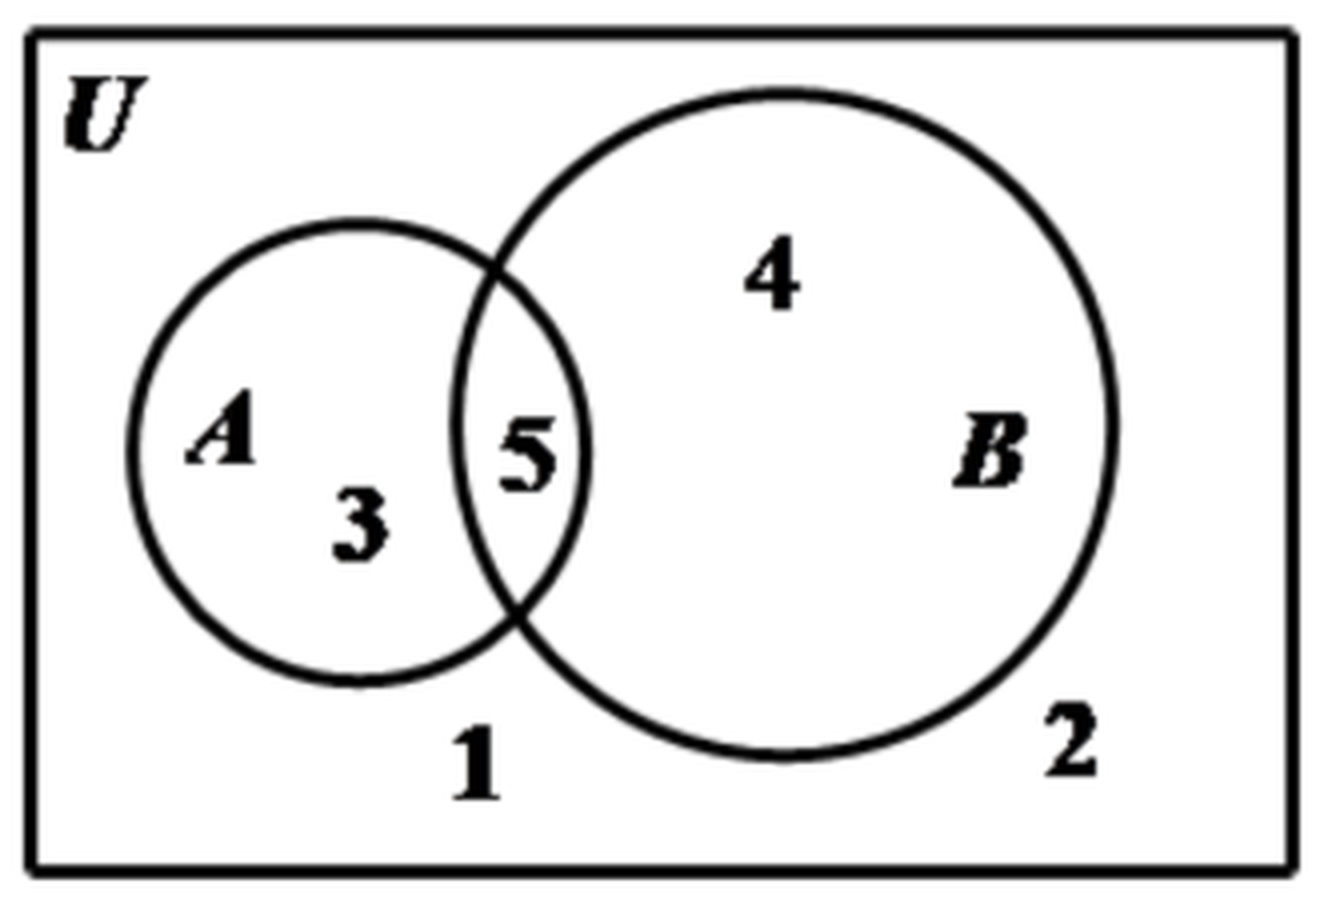
\includegraphics[width=0.28\textwidth]{figures/venn_U5_AB.png}
\end{center}

\keepwithprev
A. $3\notin A$ 且 $3\notin B$\qquad\qquad B. $3\in A$ 且 $3\in B$

C. $3\notin A$ 且 $3\in B$\qquad\qquad D. $3\in A$ 且 $3\notin B$

\ans{$D$}

\ifanswer
\solbegin
\step{画出韦恩图，得 $A=\{5,3\}$，$B=\{5,4\}$，}
\step{则 $3\in A$ 且 $3\notin B$. 故选 $D$.}
\solend

\fi

% 同第 13 题：整块（题干 + 图 + 选项）在答案版还要再挂【答案】【解析】，页末更易被拆开。
\needvspace{7.5cm}
\item 如图表示图形阴影部分的是\mbox{（\quad）}

\begin{center}
% 图取原卷截图、4× LANCZOS 放大（三圆 $A$、$B$、$C$，阴影为整个 $A$ 圆加 $B\cap C$）。
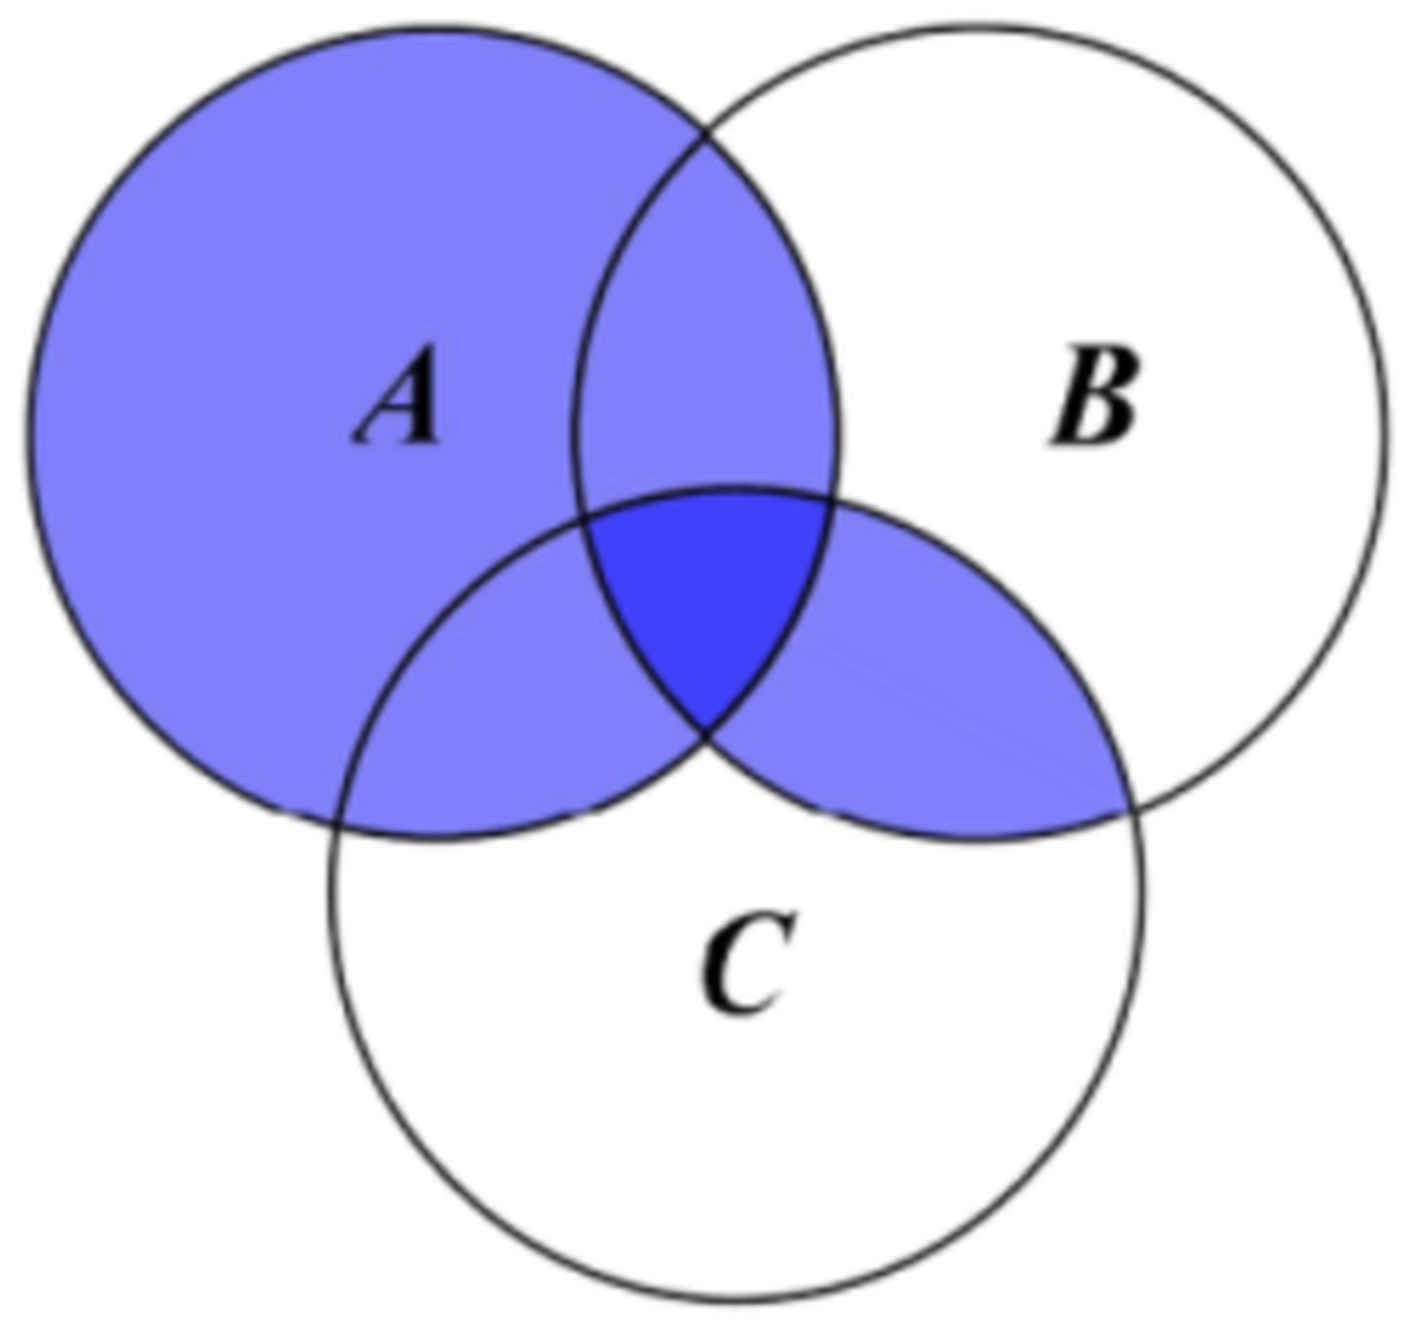
\includegraphics[width=0.30\textwidth]{figures/venn_A_union_BC.png}
\end{center}

\keepwithprev
A. $(A\cup C)\cap(B\cup C)$\qquad\qquad B. $(A\cup B)\cap(A\cup C)$

C. $(A\cup B)\cap(B\cup C)$\qquad\qquad D. $(A\cup B)\cap C$

\ans{$B$}

\ifanswer
\solbegin
\step{图中阴影部分表示元素满足是 $A$ 中的元素，或者是 $B$ 与 $C$ 的公共元素，}
\step{故可以表示为 $A\cup(B\cap C)$，也可以表示为 $(A\cup B)\cap(A\cup C)$.
故选 $B$.}
\solend

\fi

\item 设集合 $M=\left\{x\mid m\leqslant x\leqslant m+\dfrac34\right\}$，
$N=\left\{x\mid n-\dfrac13\leqslant x\leqslant n\right\}$，且 $M$、$N$ 都是集合
$\{x\mid0\leqslant x\leqslant1\}$ 的子集，如果把 $b-a$ 叫做集合
$\{x\mid a\leqslant x\leqslant b\}$ 的“长度”，那么集合 $M\cap N$ 的“长度”的
最小值是\mbox{（\quad）}

\keepwithprev
A. $\dfrac23$\qquad B. $\dfrac1{12}$\qquad C. $\dfrac13$\qquad D. $\dfrac5{12}$

\ans{$B$}

\ifanswer
\solbegin
\step{$M$ 的长度为 $\dfrac34$，$N$ 的长度为 $\dfrac13$，}
\step{当集合 $M\cap N$ 的长度的最小值时，$M$ 与 $N$ 应分别在区间 $[0,1]$ 的左右两端，}
\step{故 $M\cap N$ 的长度的最小值是 $\dfrac34+\dfrac13-1=\dfrac1{12}$，故选 $B$.}
\solend

\fi

\item 定义集合运算 $A-B=\{x\mid x\in A\text{ 且 }x\notin B\}$ 称为集合 $A$ 与集合 $B$ 的
差集；定义集合运算 $A\Delta B=(A-B)\cup(B-A)$ 称为集合 $A$ 与集合 $B$ 的对称差，
有以下 $4$ 个等式：① $A\Delta B=B\Delta A$；② $(A\Delta B)\Delta C=A\Delta(B\Delta C)$；
③ $A\cap(B\Delta C)=(A\cap B)\Delta(A\cap C)$；
④ $A\cup(B\Delta C)=(A\cup B)\Delta(A\cup C)$，
则 $4$ 个等式中恒成立的是\mbox{（\quad）}

\keepwithprev
A. ①②\qquad B. ①②③\qquad C. ①②④\qquad D. ①②③④

\ans{$B$}

\ifanswer
\solbegin
\step{对于①，由 $B\Delta A=(B-A)\cup(A-B)=(A-B)\cup(B-A)=A\Delta B$，
所以①正确；}
\step{对于②，由 $A-B=\{x\mid x\in A\text{ 且 }x\notin B\}
=\{x\mid x\in A,x\notin(A\cap B)\}=A-(A\cap B)$，}
\step{同理可得 $B-A=B-(A\cap B)$，}
\step{则 $A\Delta B=(A-B)\cup(B-A)=(A\cup B)-(A\cap B)$，}
\step{所以 $(A\Delta B)\Delta C=(A\Delta B)\cup C-(A\Delta B)\cap C$，}
\step{所以表示的集合为图（1）中阴影部分所表示的集合，如图所示，}
\step{同理 $A\Delta(B\Delta C)=A\cup(B\Delta C)-A\cap(B\Delta C)$，
也表示图（1）中阴影部分所表示的集合，}
\step{所以 $(A\Delta B)\Delta C=A\Delta(B\Delta C)$，所以②正确；}

\begin{center}
% 图取原卷截图、4× LANCZOS 放大（原卷印在下一页顶部，共三幅三圆韦恩图：
% 图（1）一幅、图（2）左右两幅，图（2）两幅下方各有一行式子标注）。
% 图只在【解析】里出现，故放进 \ifanswer 块，试卷版不排。
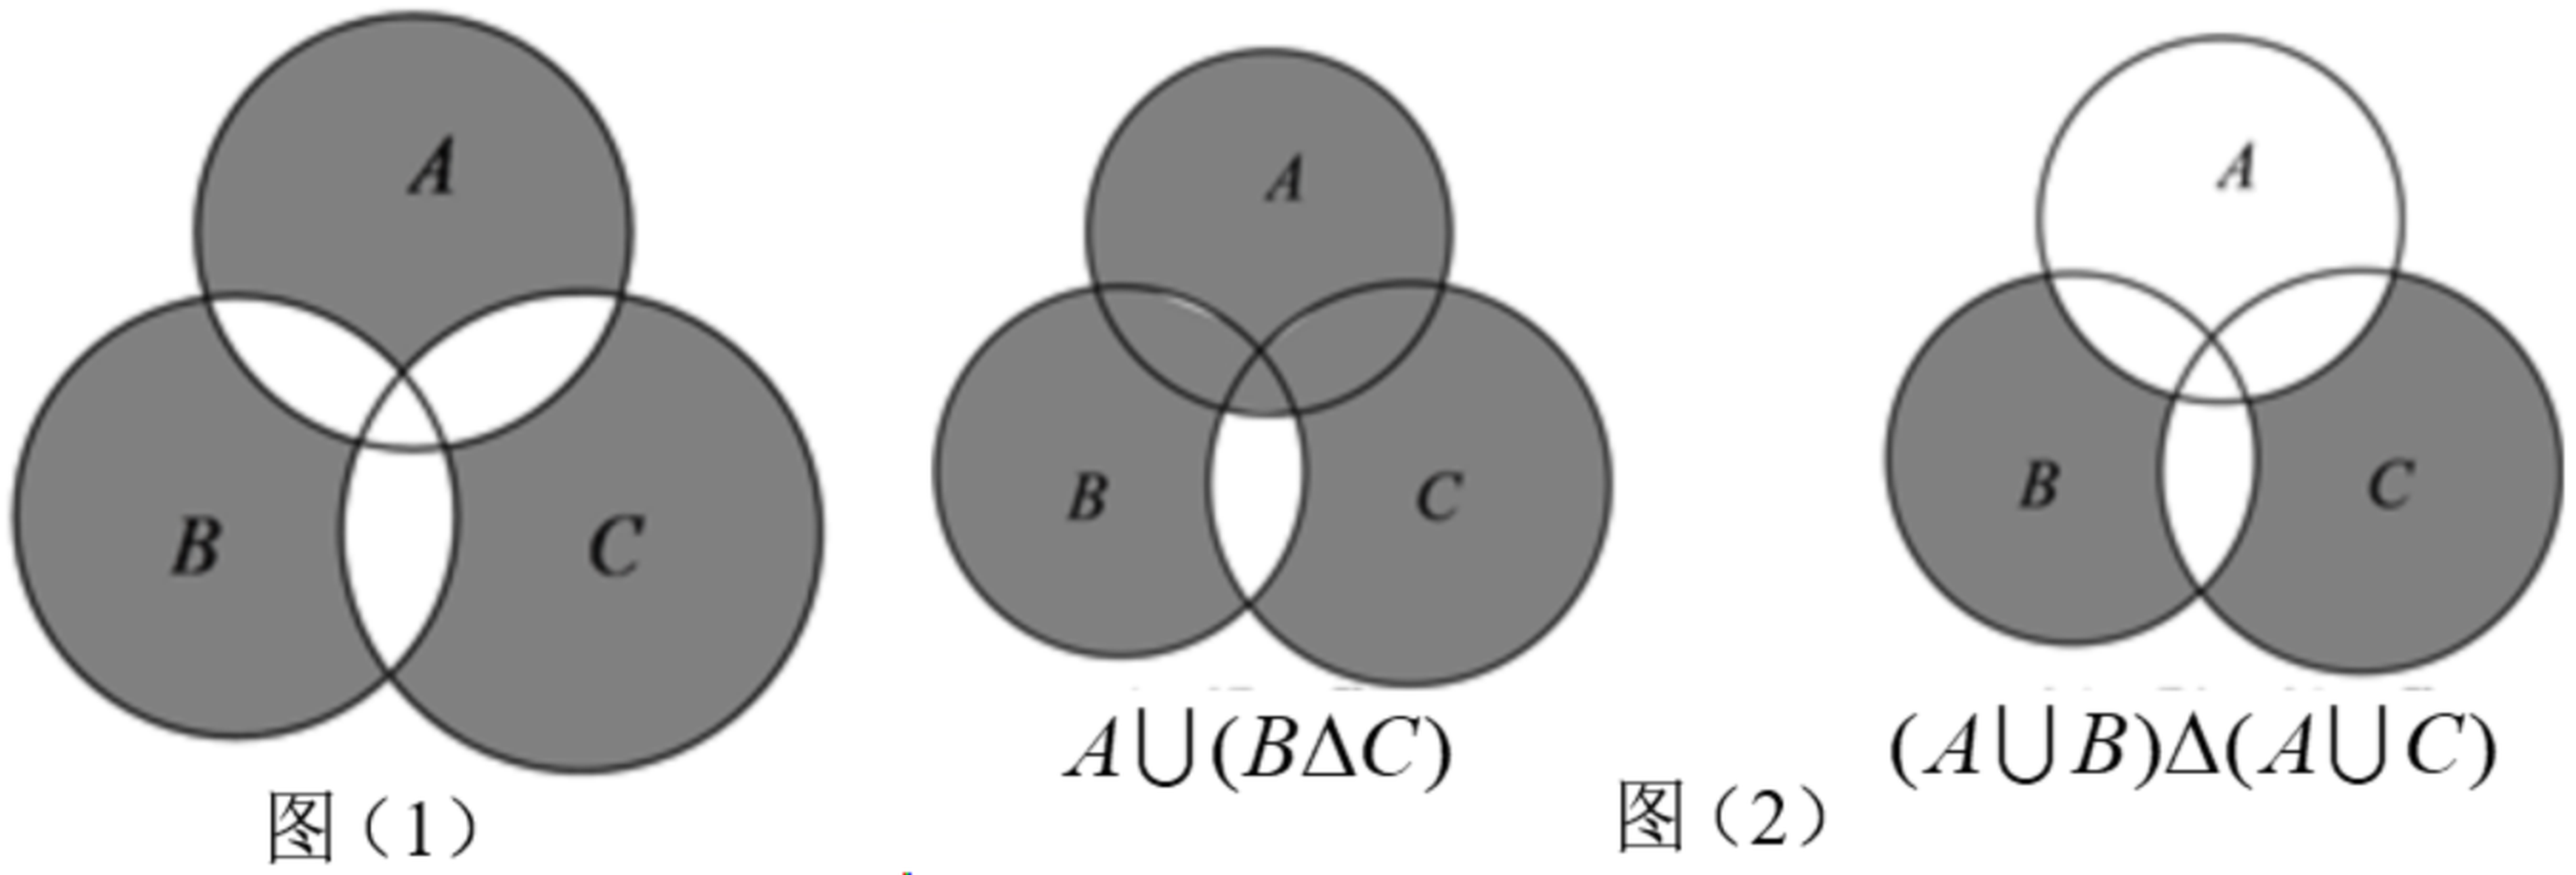
\includegraphics[width=0.86\textwidth]{figures/venn_symdiff3.png}
\end{center}

\step{对于③，由 $A\cap(B\Delta C)=A\cap(B\cup C-B\cap C)
=A\cap(B\cup C)-A\cap(B\cap C)$}
\step{$=(A\cap B)\cup(A\cap C)-(A\cap B)\cap(A\cap C)=(A\cap B)\Delta(A\cap C)$，
所以③正确；}
\step{对于④，如图（2）所示，$A\cup(B\Delta C)\neq(A\cup B)\Delta(A\cup C)$，
所以④错误.}
\step{故选 $B$.}
\solend

\fi

\end{enumerate}

\bigsec{三、解答题}

\begin{enumerate}
\setcounter{enumi}{16}

\item 已知集合 $M=\{x\mid a-1\leqslant x\leqslant2a+3\}$，$P=\{x\mid-2<x\leqslant4\}$，
全集 $U=\R$.

\begin{enumerate}[label=(\arabic*)]
\item 当 $a=2$ 时，求 $M\cap P$；
\item 若 $x\in P$ 是 $x\in M$ 的必要不充分条件，求实数 $a$ 的取值范围.
\end{enumerate}

\ifanswer
\solbegin
\stepm{(1)}{当 $a=2$ 时，集合 $M=\{x\mid1\leqslant x\leqslant7\}$，}
\step{所以 $M\cap P=\{x\mid1\leqslant x\leqslant4\}$；}
\stepm{(2)}{因为 $x\in P$ 是 $x\in M$ 的必要不充分条件，所以 $M\subset P$，}
\step{当 $M=\varnothing$ 时，$a-1>2a+3$，解得 $a<-4$，}
\step{当 $M\neq\varnothing$ 时，则
$\begin{cases}a-1\leqslant2a+3\\ a-1>-2\\ 2a+3\leqslant4\end{cases}$，
解得 $-1<a\leqslant\dfrac12$，}
\step{综上所述，实数 $a$ 的取值范围为
$(-\infty,-4)\cup\left(-1,\dfrac12\right]$.}
\solend

\fi

\ansspace[6]

\item 一辆汽车在某段路程中的行驶速度与时间的关系如图：

\begin{center}
% 图取原卷截图、4× LANCZOS 放大（速度—时间图：纵轴 $v/(\mathrm{km/h})$、
% 横轴 $t(\mathrm{h})$，$t\in[0,1]$、$[1,2]$、$[2,3]$ 三段矩形条高 50、80、90）。
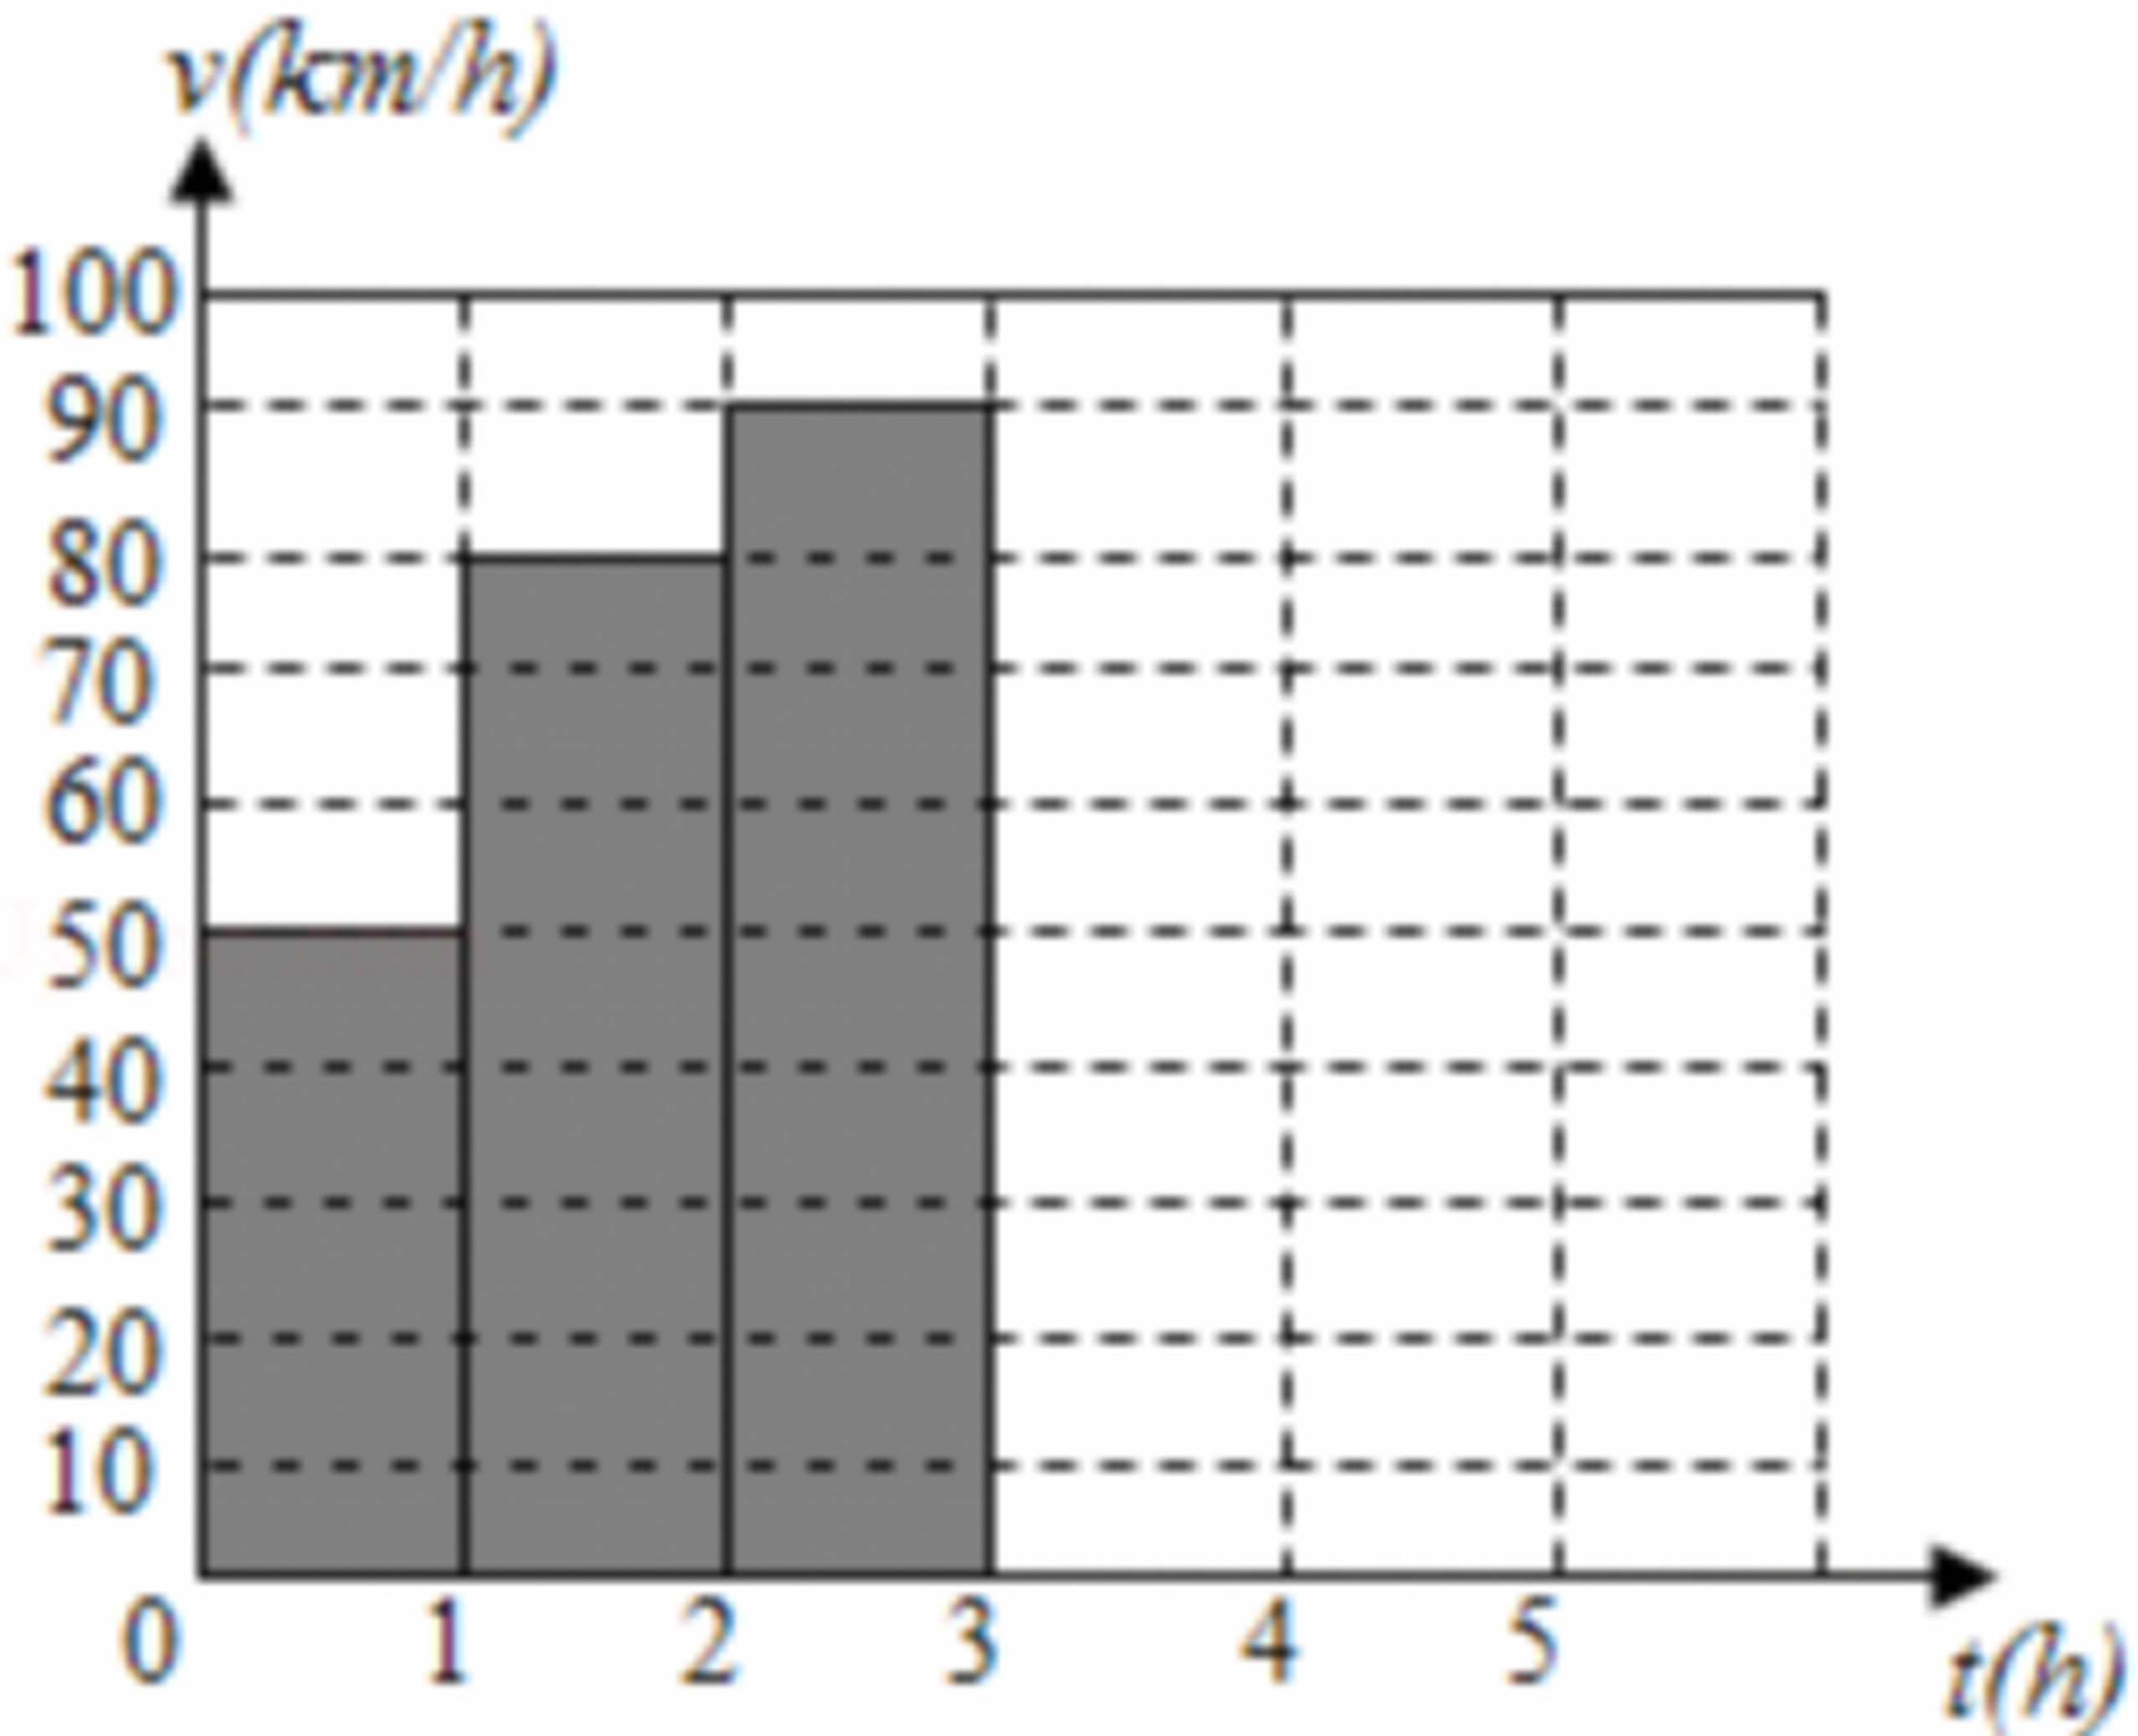
\includegraphics[width=0.52\textwidth]{figures/speed_time_bars.png}
\end{center}

\begin{enumerate}[label=(\arabic*)]
\item 求图中阴影部分的面积，并说明所求面积的实际意义；
\item 假设这辆汽车的里程表在汽车行驶这段路程前的读数为 $2004\,\mathrm{km}$，
试将汽车行驶这段路程时汽车里程表读数 $S$ 表示为时间 $t$ 的函数，
并求出当汽车里程表读数为 $2094\,\mathrm{km}$ 时，汽车行驶了多少时间？
\end{enumerate}

\ifanswer
\solbegin
\stepm{(1)}{由一辆汽车在某段路程中的行驶速度与时间的关系图，}
\step{得阴影部分的面积为 $50\times1+80\times1+90\times1=220$，}
\step{阴影部分的面积表示汽车在 $3$ 小时内行驶的路程为 $220\,\mathrm{km}$.}
\stepm{(2)}{$S=\begin{cases}
50t+2004,&0\leqslant t<1\\
80(t-1)+2054,&1\leqslant t<2\\
90(t-2)+2134,&2\leqslant t\leqslant3
\end{cases}$}
\step{令 $80(t-1)+2054=2094$，解得 $t=1.5$，所以汽车行驶 $1.5$ 小时.}
\solend

\fi

\ansspace[6]

\item 已知集合 $A=\{x\mid x<-2\text{ 或 }x\geqslant3\}$，$U=\R$.

\begin{enumerate}[label=(\arabic*)]
\item 求 $\overline{A}$；
\item 若 $B=\{x\mid mx-1>0\}$，当 $B\sub A$ 时，求实数 $m$ 的取值范围；
\item 若 $B=\{x\mid2m-6\leqslant x\leqslant m+4\}$，当 $B\cap\overline{A}=\varnothing$ 时，
求实数 $m$ 的取值范围.
\end{enumerate}

\ifanswer
\solbegin
\stepm{(1)}{因为集合 $A=\{x\mid x<-2\text{ 或 }x\geqslant3\}$，$U=\R$，
所以 $\overline{A}=\{x\mid-2\leqslant x<3\}$；}
\stepm{(2)}{当 $m=0$ 时，$B=\varnothing$，符合题意，}
\step{当 $m>0$ 时，$B=\left\{x\mid x>\dfrac1m\right\}$，则 $\dfrac1m\geqslant3$，
解得 $0<m\leqslant\dfrac13$，}
\step{当 $m<0$ 时，$B=\left\{x\mid x<\dfrac1m\right\}$，则 $\dfrac1m\leqslant-2$，
解得 $-\dfrac12\leqslant m<0$，}
\step{综上所述，实数 $m$ 的取值范围 $\left[-\dfrac12,\dfrac13\right]$；}
\stepm{(3)}{由题意得 $B=\{x\mid2m-6\leqslant x\leqslant m+4\}$，
$\overline{A}=\{x\mid-2\leqslant x<3\}$，且 $B\cap\overline{A}=\varnothing$，}
\step{当 $B=\varnothing$ 时，$2m-6>m+4$，解得 $m>10$，}
\step{当 $B\neq\varnothing$ 时，则 $\begin{cases}2m-6\leqslant m+4\\ m+4<-2\end{cases}$
或 $\begin{cases}2m-6\leqslant m+4\\ 2m-6\geqslant3\end{cases}$，}
\step{解得 $m<-6$ 或 $\dfrac92\leqslant m\leqslant10$，}
\step{综上所述，实数 $m$ 的取值范围为
$(-\infty,-6)\cup\left[\dfrac92,+\infty\right)$.}
\solend

\fi

\ansspace[8]

\item 在等腰梯形 $ABCD$ 中，$AB=DC=5$，$AD=4$，$BC=10$. 点 $E$ 在下底边 $BC$ 上.
点 $F$ 在腰 $AB$ 上.

\begin{center}
% 图取原卷截图、4× LANCZOS 放大（等腰梯形 $ABCD$ 与线段 $FE$，无辅助线）。
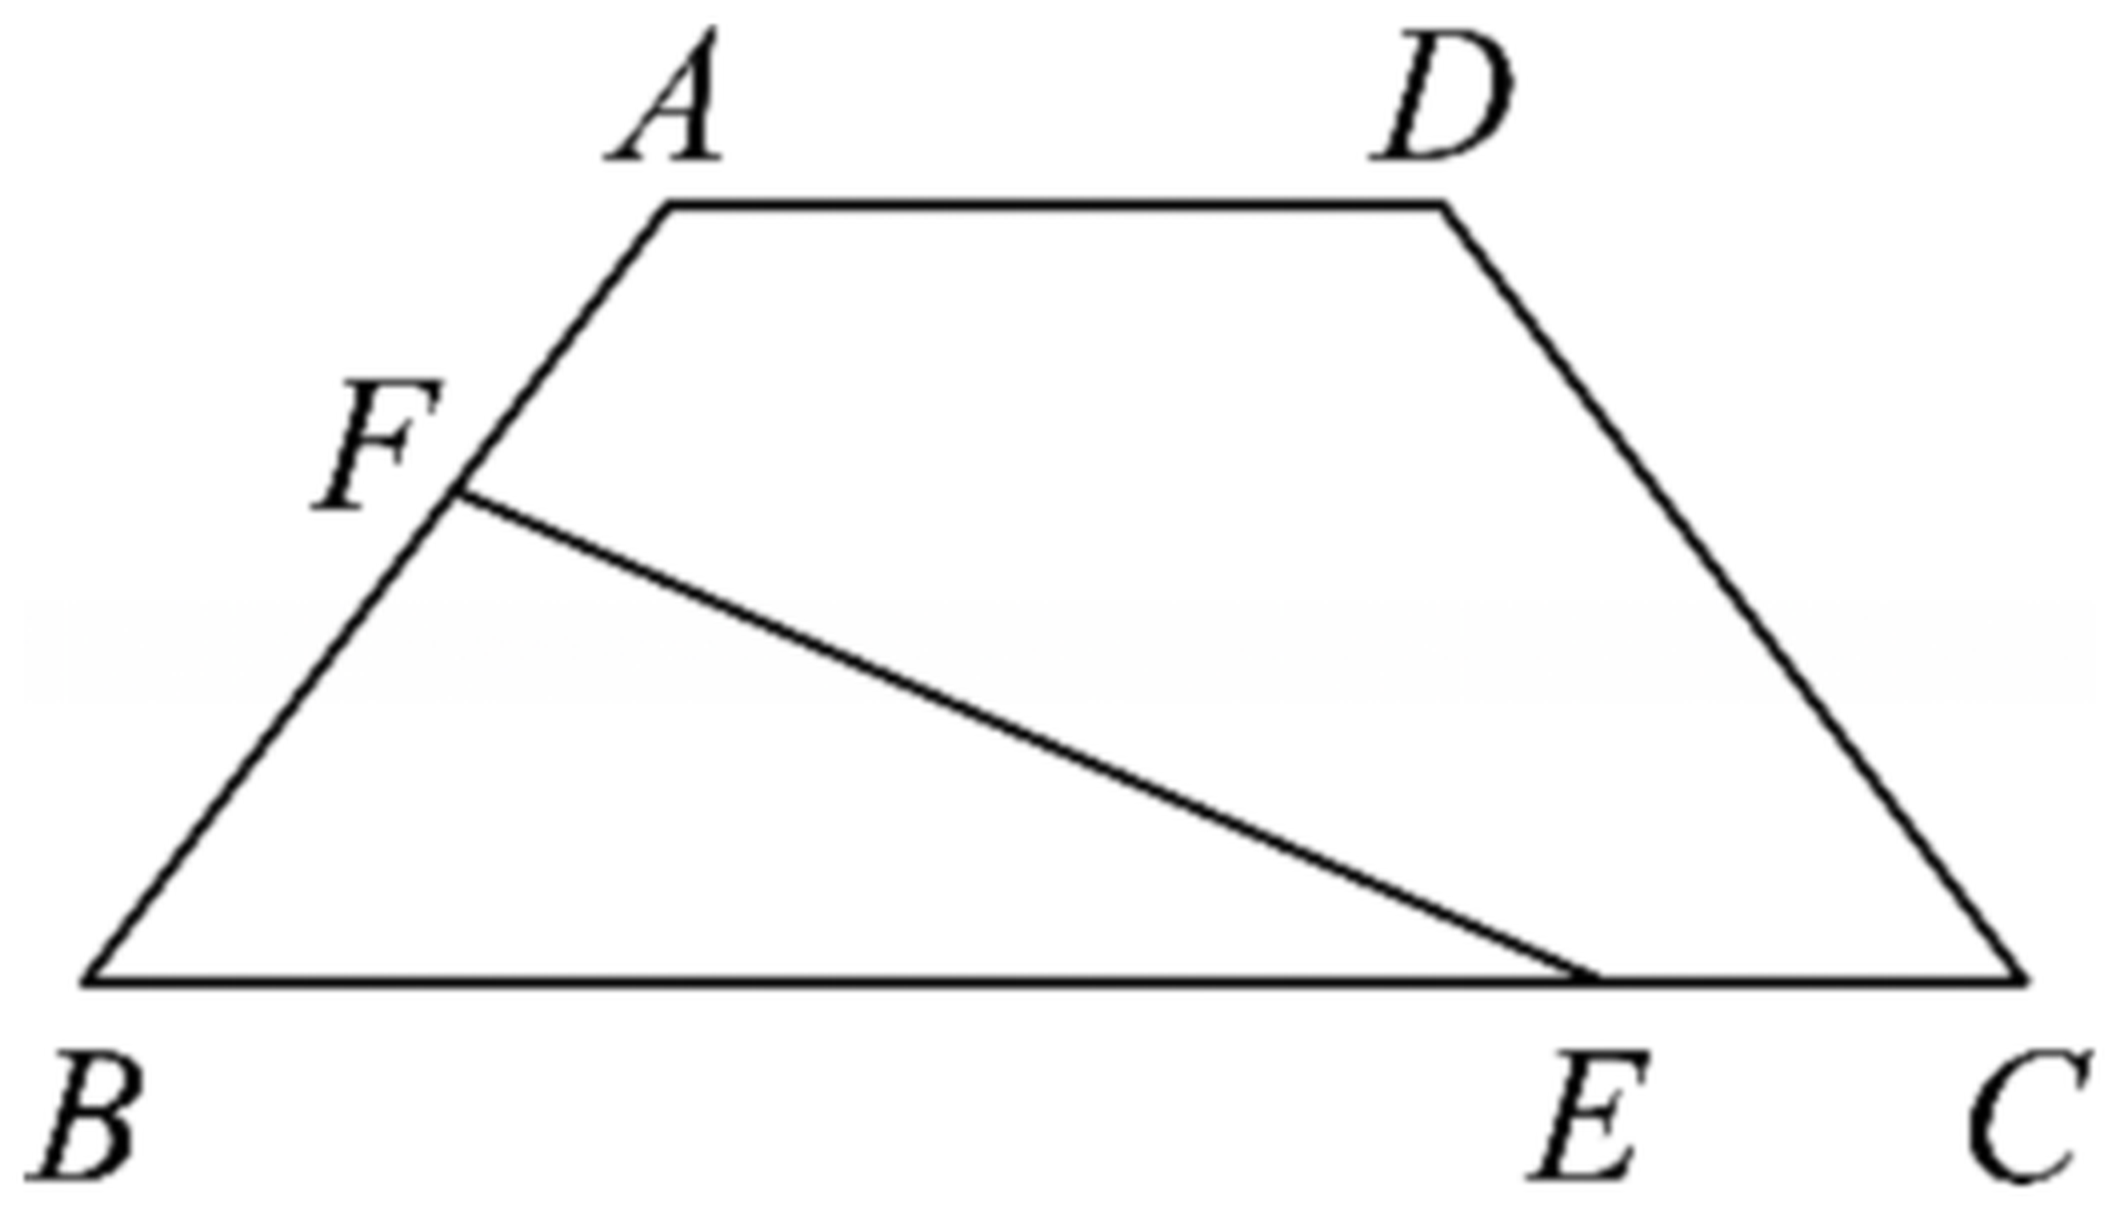
\includegraphics[width=0.46\textwidth]{figures/trapezoid_EF.png}
\end{center}

\begin{enumerate}[label=(\arabic*)]
\item 若 $EF$ 平分等腰梯形 $ABCD$ 的周长，设 $BE$ 长为 $x$，试用含 $x$ 的代数式表示
$\triangle BEF$ 的面积；
\item 是否存在线段 $EF$ 将等腰梯形 $ABCD$ 的周长和面积同时平分？若存在，求出此时 $BE$
的长；若不存在，请说明理由；
\item 是否存在线段 $EF$ 将等腰梯形 $ABCD$ 的周长和面积同时分成 $1:2$ 的两部分？
若存在，求此时 $BE$ 的长；若不存在，请说明理由.
\end{enumerate}

\ifanswer
\solbegin
\stepm{(1)}{过 $A$ 作 $AK\perp BC$ 交 $BC$ 于点 $K$，过 $F$ 作 $FG\perp BC$ 交 $BC$ 于点
$G$，}

\begin{center}
% 图取原卷截图、4× LANCZOS 放大（同梯形，多出虚线 $FG\perp BC$ 与 $AK\perp BC$
% 及两处直角符号；图只在【解析】里出现，故放进 \ifanswer 块）。
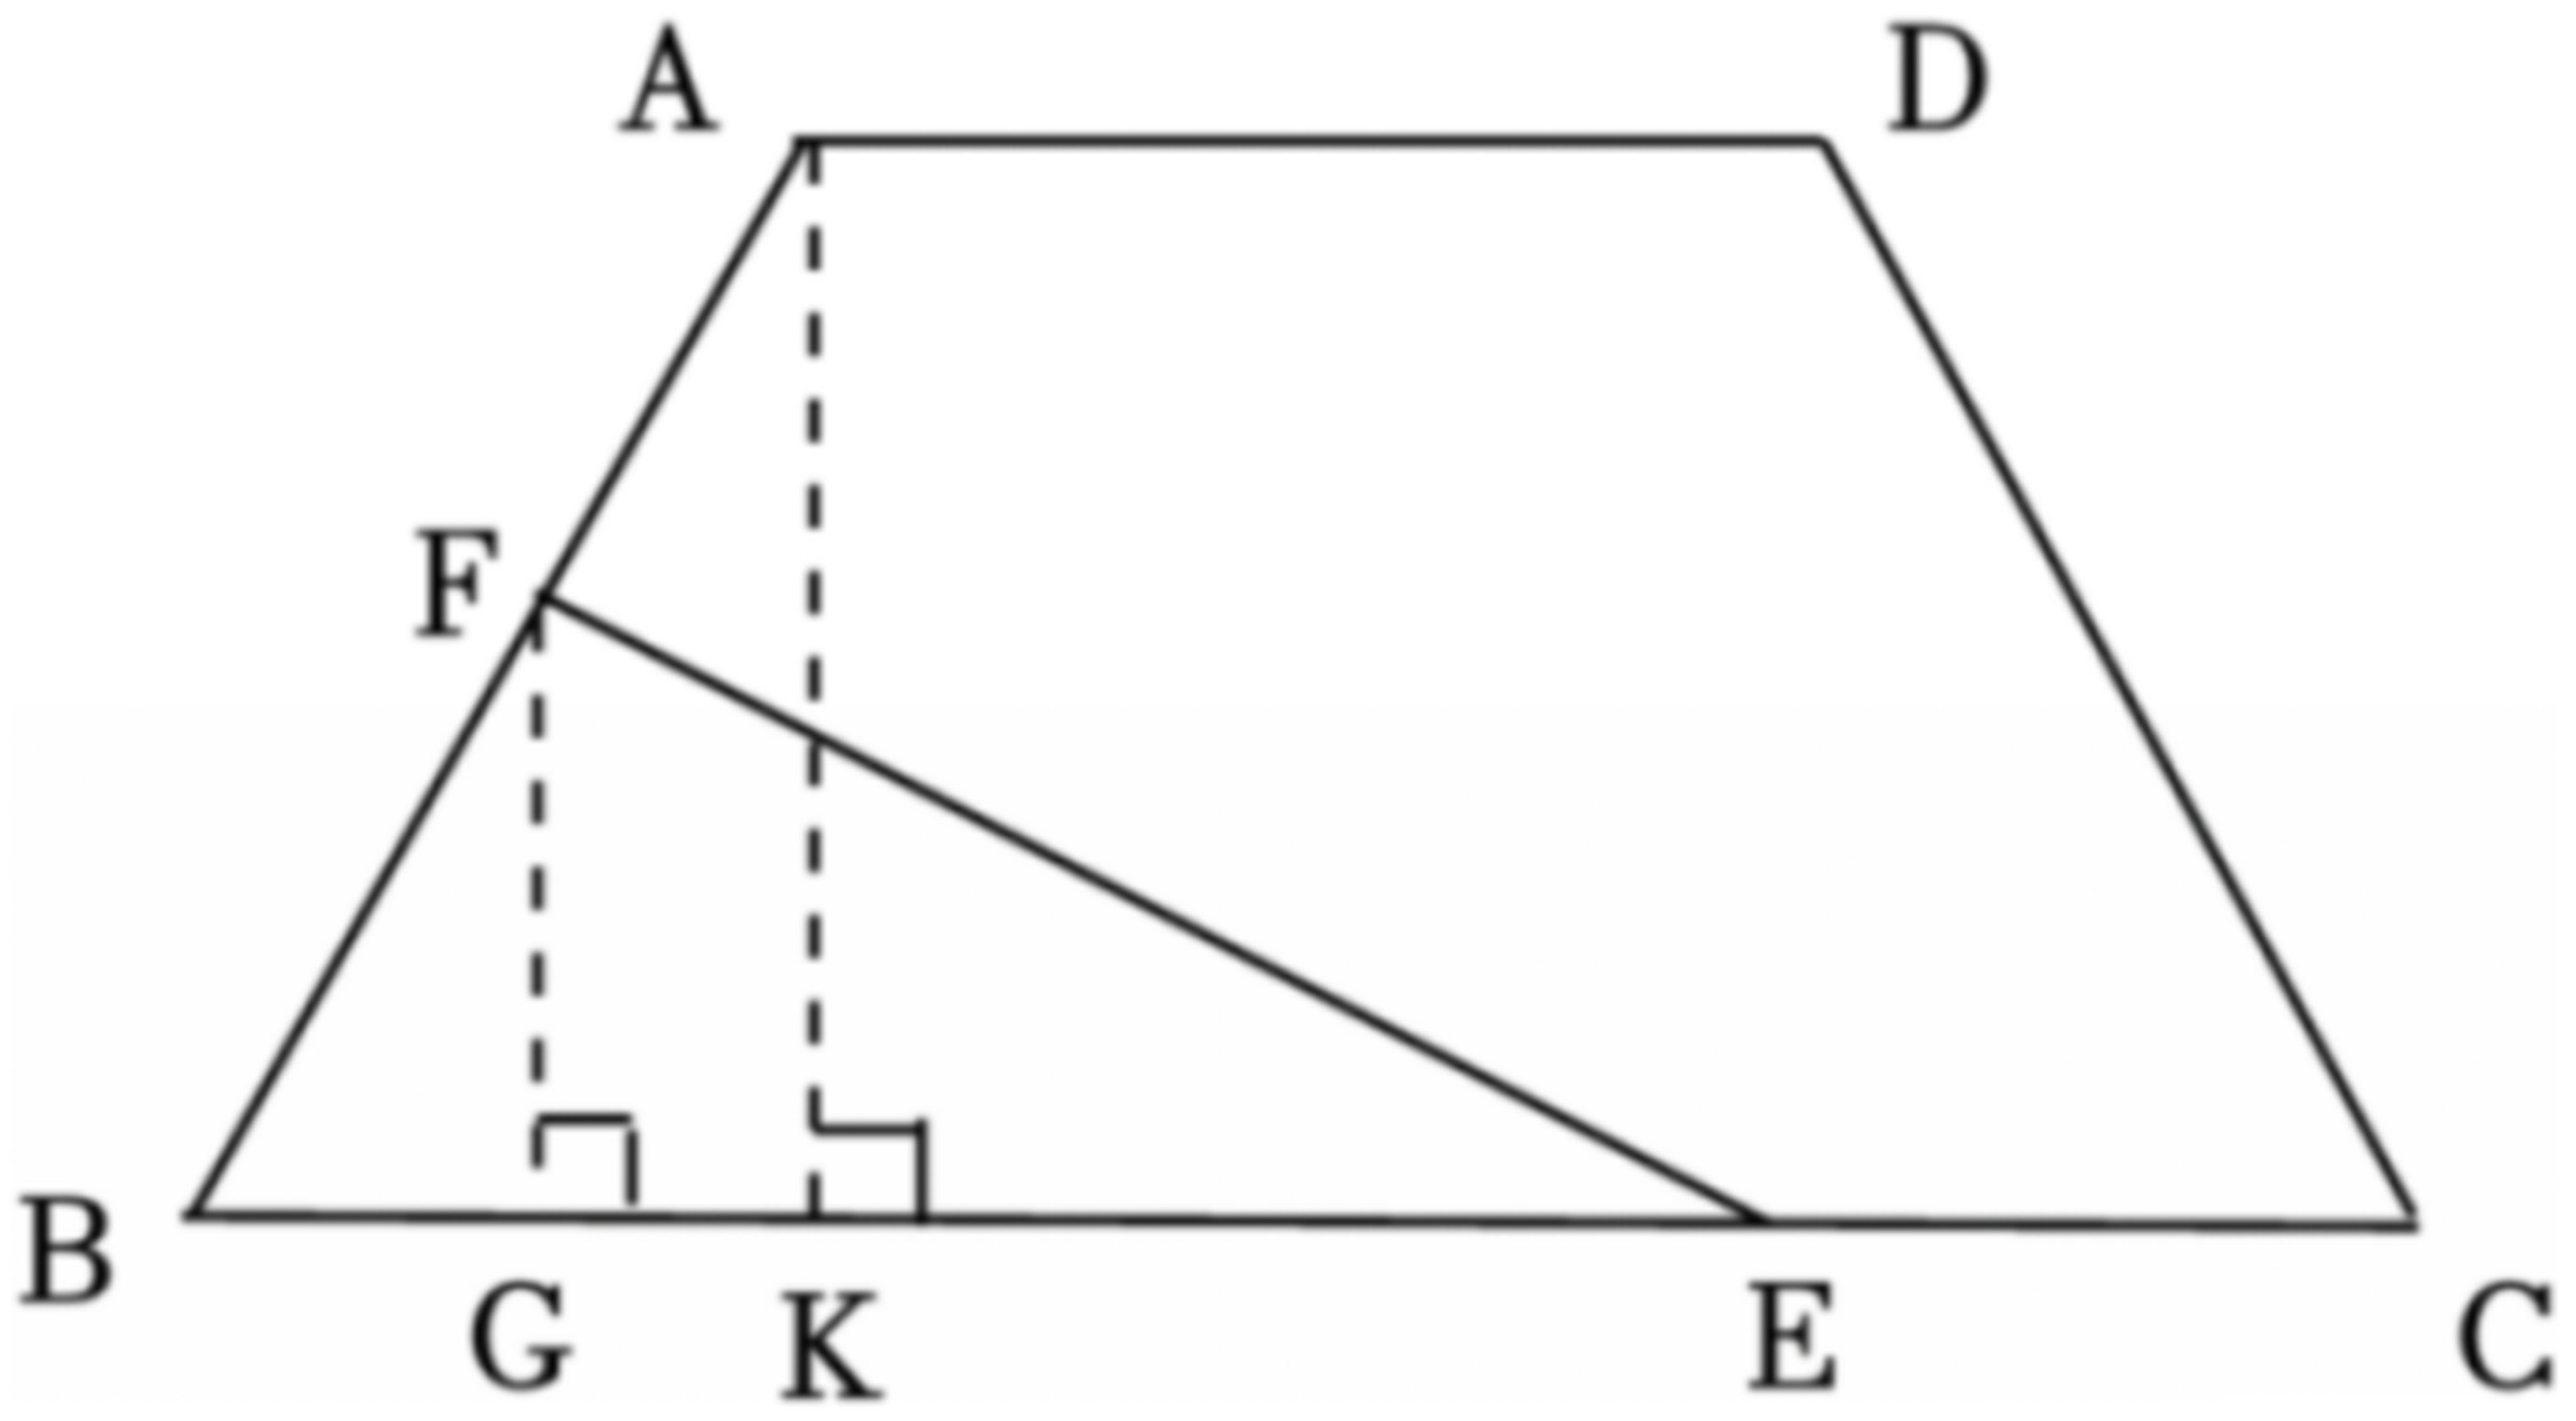
\includegraphics[width=0.62\textwidth]{figures/trapezoid_EF_aux.png}
\end{center}

\step{所以 $BK=\dfrac12\times(BC-AD)=\dfrac12\times(10-4)=3$，}
\step{$AK=\sqrt{AB^2-BK^2}=\sqrt{5^2-3^2}=4$，}
\step{由题意得，梯形 $ABCD$ 周长为 $24$，高为 $4$，面积为 $28$，}
\step{因为 $EF$ 平分等腰梯形 $ABCD$ 的周长，设 $BE$ 长为 $x$，则 $BF=12-x$，}
\step{由 $\begin{cases}0\leqslant12-x\leqslant5\\ 0\leqslant x\leqslant10\end{cases}$，
解得 $7\leqslant x\leqslant10$，}
\step{由题意得 $\triangle BFG\backsim\triangle BAK$，所以 $\dfrac{FG}{AK}=\dfrac{BF}{BA}$，
即 $\dfrac{FG}4=\dfrac{12-x}5$，}
\step{解得 $FG=\dfrac45(12-x)$，}
\step{所以 $S_{\triangle BEF}=\dfrac12BE\cdot FG
=-\dfrac25x^2+\dfrac{24}5x$（$7\leqslant x\leqslant10$）；}
\stepm{(2)}{存在，由 (1) 得 $-\dfrac25x^2+\dfrac{24}5x=\dfrac{28}2$，$x\in[7,10]$，}
\step{即 $x^2-12x+35=0$，解得 $x=7$ 或 $x=5$（舍去），}
\step{所以存在线段 $EF$ 将等腰梯形 $ABCD$ 的周长和面积同时平分，此时 $BE=7$；}
\stepm{(3)}{不存在，}
\step{情况一：$\triangle BEF$ 的面积$:$多边形 $AFECD$ 的面积 $=1:2$，
$(BE+BF):(AF+AD+DC+CE)=1:2$，}
\step{梯形周长的 $\dfrac13$ 是 $\dfrac{24}3=8$，面积的 $\dfrac13$ 是 $\dfrac{28}3$，}
\step{又因为 $BE=x$，所以 $BF=8-x$，}
\step{又因为 $\dfrac{FG}{AK}=\dfrac{BF}{BA}$，即 $\dfrac{FG}4=\dfrac{8-x}5$，
所以 $FG=\dfrac{32-4x}5$，}
\step{所以 $S_{\triangle BEF}=\dfrac12BE\times FG=-\dfrac25x^2+\dfrac{16}5x$，
所以 $\dfrac{28}3=-\dfrac25x^2+\dfrac{16}5x$，}
\step{整理得 $-3x^2+24x-70=0$，此时 $\Delta<0$，无解，故不存在；}
\step{情况二：$\triangle BEF$ 的面积$:$多边形 $AFECD$ 的面积 $=2:1$，
$(BE+BF):(AF+AD+DC+CE)=2:1$，}
\step{梯形周长的 $\dfrac13$ 为 $\dfrac{24}3=8$，面积的 $\dfrac13$ 为 $\dfrac{28}3$，
又 $BE=x$，所以 $BF=16-x$，}
\step{又 $\dfrac{FG}{AK}=\dfrac{BF}{BA}$，即 $\dfrac{FG}4=\dfrac{16-x}5$，
所以 $FG=\dfrac{64-4x}5$，}
\step{所以 $S_{\triangle BEF}=\dfrac12BE\times FG=-\dfrac25x^2+\dfrac{32}5x$，}
\step{所以 $\dfrac{28}3\times2=-\dfrac25x^2+\dfrac{32}5x$，
整理得 $-3x^2+48x-140=0$，}
\step{解得 $x=\dfrac{48+\sqrt{624}}6>10$，$x=\dfrac{48-\sqrt{624}}6<7$，
不符合题意，舍去，故不存在；}
\step{综上所述，不存在线段 $EF$ 将等腰梯形 $ABCD$ 的周长和面积同时分成 $1:2$ 的两部分.}
\solend

\fi

\ansspace[8]

\item 对集合 $\{1,2,\cdots,n\}$ 及其每一个非空子集 $A$，定义一个唯一确定的“交替和”
如下：将 $A$ 中的元素按照递减的次序排列，然后将第一个元素交替地减或加后继的元素所得的
结果，例如，子集 $\{1,2,4,6,9\}$ 的“交替和”是 $9-6+4-2+1=6$，子集 $\{5,6\}$ 的
“交替和”是 $6-5=1$，子集 $\{2\}$ 的交替和是 $2$；定义一个唯一确定的“交替积”如下：
将 $A$ 中的元素按照递减的次序排列，然后将第一个元素交替地除以或乘以后继的数所得的结果，
例如，集合 $\{1,2,4,6,9\}$ 的“交替积”是 $9\div6\times4\div2\times1=3$，
$\{5,6\}$ 的“交替积”是 $6\div5=1.2$，$\{2\}$ 的“交替积”是 $2$.

\begin{enumerate}[label=(\arabic*)]
\item 对于 $\{1,2,3,4,5,6,7,8,9\}$，求其所有子集的“交替和”的总和；
\item 对于 $\{1,2,\cdots,n\}$，求其所有子集的“交替和”的总和；
\item 对于 $\left\{n\mid\dfrac{495}{n+2}\in\N,n\in\Z\right\}$ 求其所有子集的
“交替积”的总和.
\end{enumerate}

\ifanswer
\solbegin
\stepm{(1)}{集合 $\{1,2,3,4,5,6,7,8,9\}$ 的子集中，除去 $\{9\}$ 外还有 $2^9-2$ 个
非空子集，}
\step{把这 $2^9-2$ 个非空子集两两组合后分别计算每一组中“交替和”之和，}
\step{组合原则是设 $A_i=\{9,a_1,a_2,\cdots\}$，$A_i^1=\{a_1,a_2,\cdots\}$，}
\step{集合 $A_i^1$ 的元素为集合 $A_i$ 中去掉 $9$ 的所有元素，把 $A_i$ 和 $A_i^1$
结合为一组，}
\step{显然，每组的“交替和”的和为 $9$，共有 $\dfrac{2^9-2}2$ 组，}
\step{所以，所有“交替和”之和应该为 $\dfrac{9(2^9-2)}2+9=2304$；}
\stepm{(2)}{集合 $\{1,2,\cdots,n\}$ 的子集中，除去 $\{n\}$ 外还有 $2^n-2$ 个非空子集，}
\step{把这 $2^n-2$ 个非空子集两两组合后分别计算每一组中“交替和”之和，}
\step{组合原则是设 $A_i=\{n,a_1,a_2,\cdots\}$，$A_i^1=\{a_1,a_2,\cdots\}$，}
\step{集合 $A_i^1$ 的元素为集合 $A_i$ 中去掉 $n$ 的所有元素，把 $A_i$ 和 $A_i^1$
结合为一组，}
\step{显然，每组的“交替和”的和为 $n$，共有 $\dfrac{2^n-2}2$ 组，}
% 注：下一行分子原卷印作花括号（其余同类处皆用圆括号），照抄未改，见文件头“原卷存疑”③。
\step{所以，所有“交替和”之和应该为 $\dfrac{n\{2^n-2\}}2+n=n\cdot2^{n-1}$；}
\stepm{(3)}{集合 $\left\{n\mid\dfrac{495}{n+2}\in\N,n\in\Z\right\}
=\{493,163,97,53,43,31,13,9,7,3,1,-1\}$，}
\step{其中除去 $\{-1\}$ 外还有 $2^{12}-2$ 个非空子集，}
% 注：下一行原卷把“把这”重复印了一次（“把这把这”），照抄未改，见文件头“原卷存疑”②。
\step{把这把这 $2^{12}-2$ 个非空子集两两组合后分别计算每一组中“交替积”之和，}
\step{组合原则是设 $A_j=\{-1,a_1,a_2,\cdots\}$，$A_j^1=\{a_1,a_2,\cdots\}$，}
\step{集合 $A_j^1$ 的元素为集合 $A_j$ 中去掉 $-1$ 的所有元素，把 $A_j$ 和 $A_j^1$
结合为一组，}
\step{显然，每组的“交替积”的和为 $0$，共有 $\dfrac{2^{12}-2}2$ 组，}
\step{所以，所有“交替积”之和应该为 $\dfrac{2^{12}-2}2\times0-1=-1$.}
\solend

\fi

\ansspace*[10]

\end{enumerate}

\end{document}
"
% 紧凑版：xelatex "\def\iscompact{1}% 高一30_南洋模范中学_开学考.tex
%   —— 高一上数学“2026-2027 年南洋模范中学高一上开学考”（试卷版/答案版）
% 试卷版：xelatex 高一30_南洋模范中学_开学考.tex
% 答案版：xelatex "\def\isanswer{1}\input{高一30_南洋模范中学_开学考.tex}"
% 紧凑版：xelatex "\def\iscompact{1}\input{高一30_南洋模范中学_开学考.tex}"
%
% 原始材料是微信公众号图文（公众号“魔都数学加油站”连载“27学年高一 30”，2026-09-23 发布，
% 原文标题“27学年高一30——2026-2027年上海市南洋模范中学高一上开学考”），
% 正文为 11 张 PNG 页。**同一篇里各页分辨率不一致**——第 2、3、9、10 页 4762×6735，
% 其余七页 2560×3620（已逐页打开确认，非下载缺档），取的是 mmbiz.qpic.cn/<hash>/0 的原图档。
% 原文本身就是一份**讲评版**：填空第 3—7 题下方印【答案】，第 8—12 题与其后各题印【解析】。
% 试题文字、答案与解析均照原卷录入，未改内容。卷面的粉色斜水印属水印，未录入。
%
% 卷首标题：原卷印作“2026-2027 年南洋模范中学高一上开学考”（公众号标题里的“上海市”
% 三字卷面标题行没有，本稿照卷面），年份区间按全稿惯例排 en dash，前缀照原卷保留“年”。
%
% 与原卷的排版差异（均已在 README“说明”中交代）：
%   ① 原文自**第 3 题**起（第 1、2 题未在该文中发布），故本稿题号亦自 3 起；
%   ② 原卷本就印有“一、填空题”“二、选择题”“三、解答题”三节标题，本稿照原卷分节，
%      只把标题改排成全稿统一的“大节标题”样式；
%   ③ 原卷填空第 3—7 题只印【答案】行、第 8 题起印【解析】（选择题答案写在解析末句
%      “故选 D／B”里），本稿统一改为试卷版隐去、答案版以 \ans{}／\ifanswer 块给出，
%      两版彻底分离；
%   ④ 子集符号原卷两种并用：第 7 题题干两处、第 19(2) 题作带下划线的 $\subseteq$，
%      第 17(2) 题解析作真包含的 $\subset$，本稿分别照录为 $\sub$ 与 $\subset$；
%   ⑤ 补集符号原卷一律作**上横线**（$\overline{A}$、$\overline{B}$），本稿照录；
%   ⑥ 原卷的实数集 R 一律作斜体（第 4 题、第 17 题与第 19 题题干的 $U=R$），
%      第 21(3) 题的自然数集与整数集作**粗体** $\mathbf{N}$、$\mathbf{Z}$，
%      本稿按全稿惯例统一写作 $\R$、$\N$、$\Z$；
%   ⑦ 原卷填空的横线约两个字宽，本稿按全稿惯例统一排 \blankline[4.4em]；
%   ⑧ 原卷未印副标题，本稿按全稿惯例补出副标题“集合与常用逻辑用语”——但本卷是开学考，
%      范围不止这一章：第 18 题是速度—时间图象题、第 20 题是等腰梯形的周长/面积平分问题，
%      副标题只标了主章节（见文末“高一30 专记”）；
%   ⑨ 第 13、14、18、20 题的图印在题干右侧、第 16 题的三幅图印在【解析】里的下一页顶部、
%      第 20 题【解析】另有一张带辅助线的图，本稿一律移至题干或解析之后；
%      图取原卷截图、4× LANCZOS 放大（见各 \includegraphics 前的注释）。
%
% 原卷存疑三处（均照抄原卷、未改，见源码中该处上方注释）：
%   ① 第 10 题【解析】验证“破晓集”时写的是 $\notin A$、$\in A$（如“$-2-2=-4\notin A$”），
%      但该处讨论的集合原题设里叫 $P$，同题②的“$x+y=2(k_1+k_2)\in A$”亦然——
%      本稿照抄未改（按文意应为 $P$）；
%   ② 第 21 题【解析】(3) 有“把这把这 $2^{12}-2$ 个非空子集”（“把这”重复印了一次）；
%   ③ 同题 (2) 的结论式分子原卷印作花括号 $\dfrac{n\{2^n-2\}}{2}$（其余同类处皆用圆括号）。

\documentclass[a4paper,11pt]{article}
\usepackage{common}

\begin{document}

\examtitlest[3]{2026--2027 年南洋模范中学高一上开学考}{集合与常用逻辑用语}

\bigsec{一、填空题}

\begin{enumerate}
\setcounter{enumi}{2}

\item 若集合 $A=\{x\mid x^2-2kx+7k=0\}$ 有且仅有三个真子集，则 $k$ 的取值范围是
\blankline[4.4em].

\ans{$(-\infty,0)\cup(7,+\infty)$}

\item “存在 $x\in\R$，使得 $x^2+2x+5=0$”的否定形式是 \blankline[4.4em].

\ans{对任何 $x\in\R$，都有 $x^2+2x+5\neq0$}

\item 下列命题中，$p$ 是 $q$ 的必要非充分条件的是 \blankline[4.4em].

① $p:x>2$ 且 $y>3$，$q:x+y>5$；

② $p$：四边形的四个角都相等，$q$：四边形是正方形.

\ans{②}

\item 若“条件 $\alpha:2\leqslant x\leqslant4$”是“条件 $\beta:3m-1\leqslant x\leqslant-m$”的
充分非必要条件，则 $m$ 的取值范围是 \blankline[4.4em].

\ans{$(-\infty,-4]$}

\item 满足 $\{1\}\sub M\sub\{1,2,4,5\}$ 的集合 $M$ 的个数为 \blankline[4.4em] 个.

\ans{$8$}

\item 已知集合 $A=\{1,2\}$，集合 $B=\{x\mid ax=6\}$，若 $A\cup B=A$，则 $a$ 的所有取值
构成的集合为 \blankline[4.4em].

\ifanswer
\solbegin
\step{因为 $A\cup B=A$，所以 $B\sub A$，}
\step{当 $a=0$ 时，$B=\varnothing$，满足 $B\sub A$；}
\step{当 $a\neq0$ 时，$B=\left\{\dfrac6a\right\}$，则 $\dfrac6a=1$ 或 $\dfrac6a=2$，
解得 $a=6$ 或 $a=3$，}
\step{综上所述，$a$ 的所有取值构成的集合为 $\{0,3,6\}$.}
\solend

\fi

\item 对于集合 $M$、$N$，定义 $M-N=\{x\mid x\in M\text{ 且 }x\notin N\}$，
$M\oplus N=(M-N)\cup(N-M)$，设 $A=\{y\mid y=|x|,x\in\R\}$，
$B=\{y\mid y=-(x-1)^2+2,x\in\R\}$，则 $A\oplus B=$ \blankline[4.4em].

\ifanswer
\solbegin
\step{由已知 $A=[0,+\infty)$，$B=(-\infty,2]$，}
\step{由于 $A-B=(2,+\infty)$，$B-A=(-\infty,0)$，}
\step{故 $A\oplus B=(A-B)\cup(B-A)=(-\infty,0)\cup(2,+\infty)$.}
\solend

\fi

\item 设 $P$ 为非空实数集满足：对任意给定的 $x$、$y\in P$（$x$、$y$ 可以相同），都有
$x+y\in P$，$x-y\in P$，$xy\in P$，则称 $P$ 为破晓集. 关于破晓集有下列结论：
①集合 $P=\{-2,-1,0,1,2\}$ 为破晓集；②集合 $P=\{x\mid x=2n,n\in\Z\}$ 为破晓集；
③若集合 $P_1$、$P_2$ 为破晓集，则 $P_1\cup P_2$ 为破晓集；④若集合 $P$ 为破晓集，
则一定有 $0\in P$；⑤若集合 $P_1$、$P_2$ 为破晓集，则 $P_1\cap P_2$ 为破晓集；
其中正确结论的序号是 \blankline[4.4em].

\ifanswer
\solbegin
% 注：以下几步原卷把该集合记作 $A$（题设里叫 $P$），照抄未改，见文件头“原卷存疑”①。
\step{对于①：$-2-2=-4\notin A$，故集合 $P=\{-2,-1,0,1,2\}$ 不为破晓集，故①错误；}
\step{②设 $x$、$y\in A$，则 $x=2k_1$，$y=2k_2$，且 $k_1$、$k_2\in\Z$，}
\step{故 $x+y=2(k_1+k_2)\in A$，$x-y=2(k_1-k_2)\in A$，$xy=4k_1k_2\in A$，}
\step{故集合 $P=\{x\mid x=2n,n\in\Z\}$ 为破晓集，故②正确；}
\step{③若集合 $P_1$、$P_2$ 为破晓集，设 $P_1=\{x\mid x=2k,k\in\Z\}$，
$P_2=\{x\mid x=3k,k\in\Z\}$，}
\step{但是 $P_1\cup P_2$ 不为破晓集，如 $x=2$，$y=3$ 时，$x+y=5$，
故 $5\notin(P_1\cup P_2)$，故③错误；}
\step{④若集合 $P$ 为破晓集，则取 $x=y$，$x-y=0\in A$，则一定有 $0\in P$，故④正确.}
\step{⑤正确；}
\step{故正确的是②④⑤.}
\solend

\fi

\item 已知集合 $M$ 的元素均为正整数，定义集合 $M$ 的“变项和”为：将 $M$ 中每个元素 $m$
都乘以 $(-1)^m$ 后再求和. 若集合 $A=\{n\mid1\leqslant n\leqslant10,n\in\N\}$，则集合 $A$
的所有非空子集的“变项和”的总和为 \blankline[4.4em].

\ifanswer
\solbegin
\step{$A$ 集合的所有非空子集中，每个元素出现的次数都是
$(2^{10}-1)-(2^9-1)=2^9$，}
\step{则集合 $A$ 的所有非空子集的“变项和”的总和为
$1\times(-1)^1\times2^9+2\times(-1)^2\times2^9+\cdots+10\times(-1)^{10}\times2^9$}
\step{$=(-1+2-3+4-\cdots-9+10)\times2^9=5\times2^9=2560$.}
\solend

\fi

\item 已知集合 $A=[t,t+1]\cup[t+4,t+9]$，$0\notin A$，存在正数 $\lambda$，使得对任意
$a\in A$，都有 $\dfrac\lambda a\in A$，则 $t$ 的值是 \blankline[4.4em].

\ifanswer
\solbegin
\step{当 $t>0$ 时，当 $a\in[t,t+1]$ 时，$\dfrac\lambda a\in[t+4,t+9]$，}
\step{当 $a\in[t+4,t+9]$ 时，$\dfrac\lambda a\in[t,t+1]$，}
\step{即当 $a=t$ 时，$\dfrac\lambda a\leqslant t+9$；当 $a=t+9$ 时，
$\dfrac\lambda a\geqslant t$，即 $\lambda=t(t+9)$；}
\step{当 $a=t+1$ 时，$\dfrac\lambda a\geqslant t+4$，当 $a=t+4$ 时，
$\dfrac\lambda a\leqslant t+1$，即 $\lambda=(t+1)(t+4)$，}
\step{所以 $t(t+9)=(t+1)(t+4)$，解得 $t=1$.}
\step{当 $t+1<0<t+4$ 时，当 $a\in[t,t+1]$ 时，$\dfrac\lambda a\in[t,t+1]$.}
\step{当 $a\in[t+4,t+9]$ 时，则 $\dfrac\lambda a\in[t+4,t+9]$，}
\step{即当 $a=t$ 时，$\dfrac\lambda a\leqslant t+1$，当 $a=t+1$ 时，
$\dfrac\lambda a\geqslant t$，即 $\lambda=t(t+1)$，}
\step{即当 $a=t+4$ 时，$\dfrac\lambda a\leqslant t+9$，当 $a=t+9$ 时，
$\dfrac\lambda a\geqslant t+4$，即 $\lambda=(t+4)(t+9)$，}
\step{所以 $t(t+1)=(t+4)(t+9)$，解得 $t=-3$.}
\step{当 $t+9<0$ 时，同理可得无解.}
\step{综上，$t$ 的值为 $1$ 或 $-3$.}
\solend

\fi

\end{enumerate}

\bigsec{二、选择题}

\begin{enumerate}
\setcounter{enumi}{12}

% 这道题是“题干 + 图 + 选项”约 6cm 的一整块，页末放不下就会被拆开（切页审计的 A 类），
% 故在题前先量一次页高：不够就把整道题干连图带选项一起挪到次页。
\needvspace{6.5cm}
\item 设 $U=\{1,2,3,4,5\}$，$A$、$B$ 都是 $U$ 的子集，且 $A\cap B=\{5\}$，
$\overline{A}\cap B=\{4\}$，$\overline{A}\cap\overline{B}=\{1,2\}$，
则以下四个判断中正确的是\mbox{（\quad）}

\begin{center}
% 图取原卷截图、4× LANCZOS 放大（原卷把图印在题干右侧，本稿移至此处，见文件头⑨）。
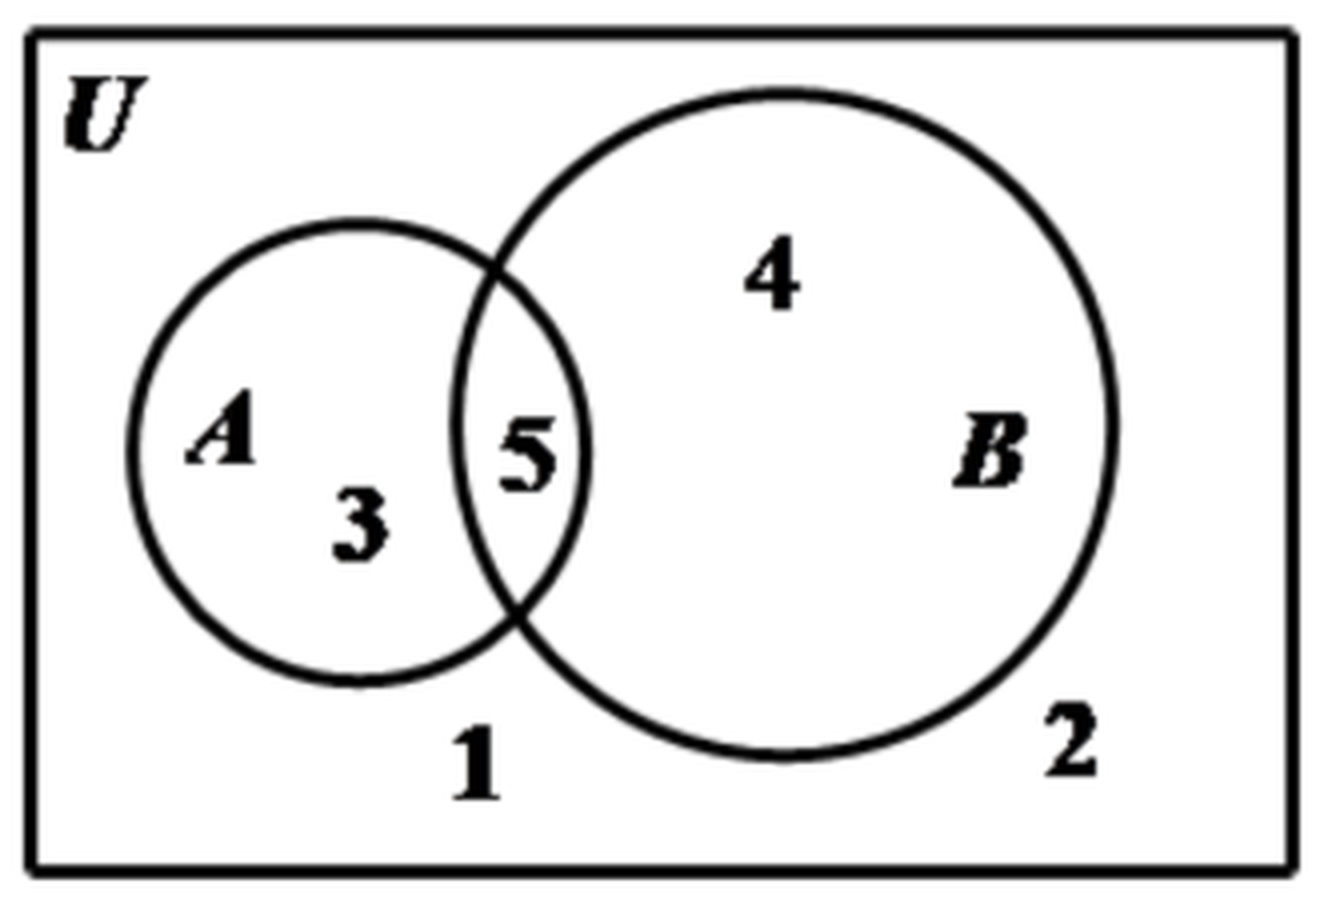
\includegraphics[width=0.28\textwidth]{figures/venn_U5_AB.png}
\end{center}

\keepwithprev
A. $3\notin A$ 且 $3\notin B$\qquad\qquad B. $3\in A$ 且 $3\in B$

C. $3\notin A$ 且 $3\in B$\qquad\qquad D. $3\in A$ 且 $3\notin B$

\ans{$D$}

\ifanswer
\solbegin
\step{画出韦恩图，得 $A=\{5,3\}$，$B=\{5,4\}$，}
\step{则 $3\in A$ 且 $3\notin B$. 故选 $D$.}
\solend

\fi

% 同第 13 题：整块（题干 + 图 + 选项）在答案版还要再挂【答案】【解析】，页末更易被拆开。
\needvspace{7.5cm}
\item 如图表示图形阴影部分的是\mbox{（\quad）}

\begin{center}
% 图取原卷截图、4× LANCZOS 放大（三圆 $A$、$B$、$C$，阴影为整个 $A$ 圆加 $B\cap C$）。
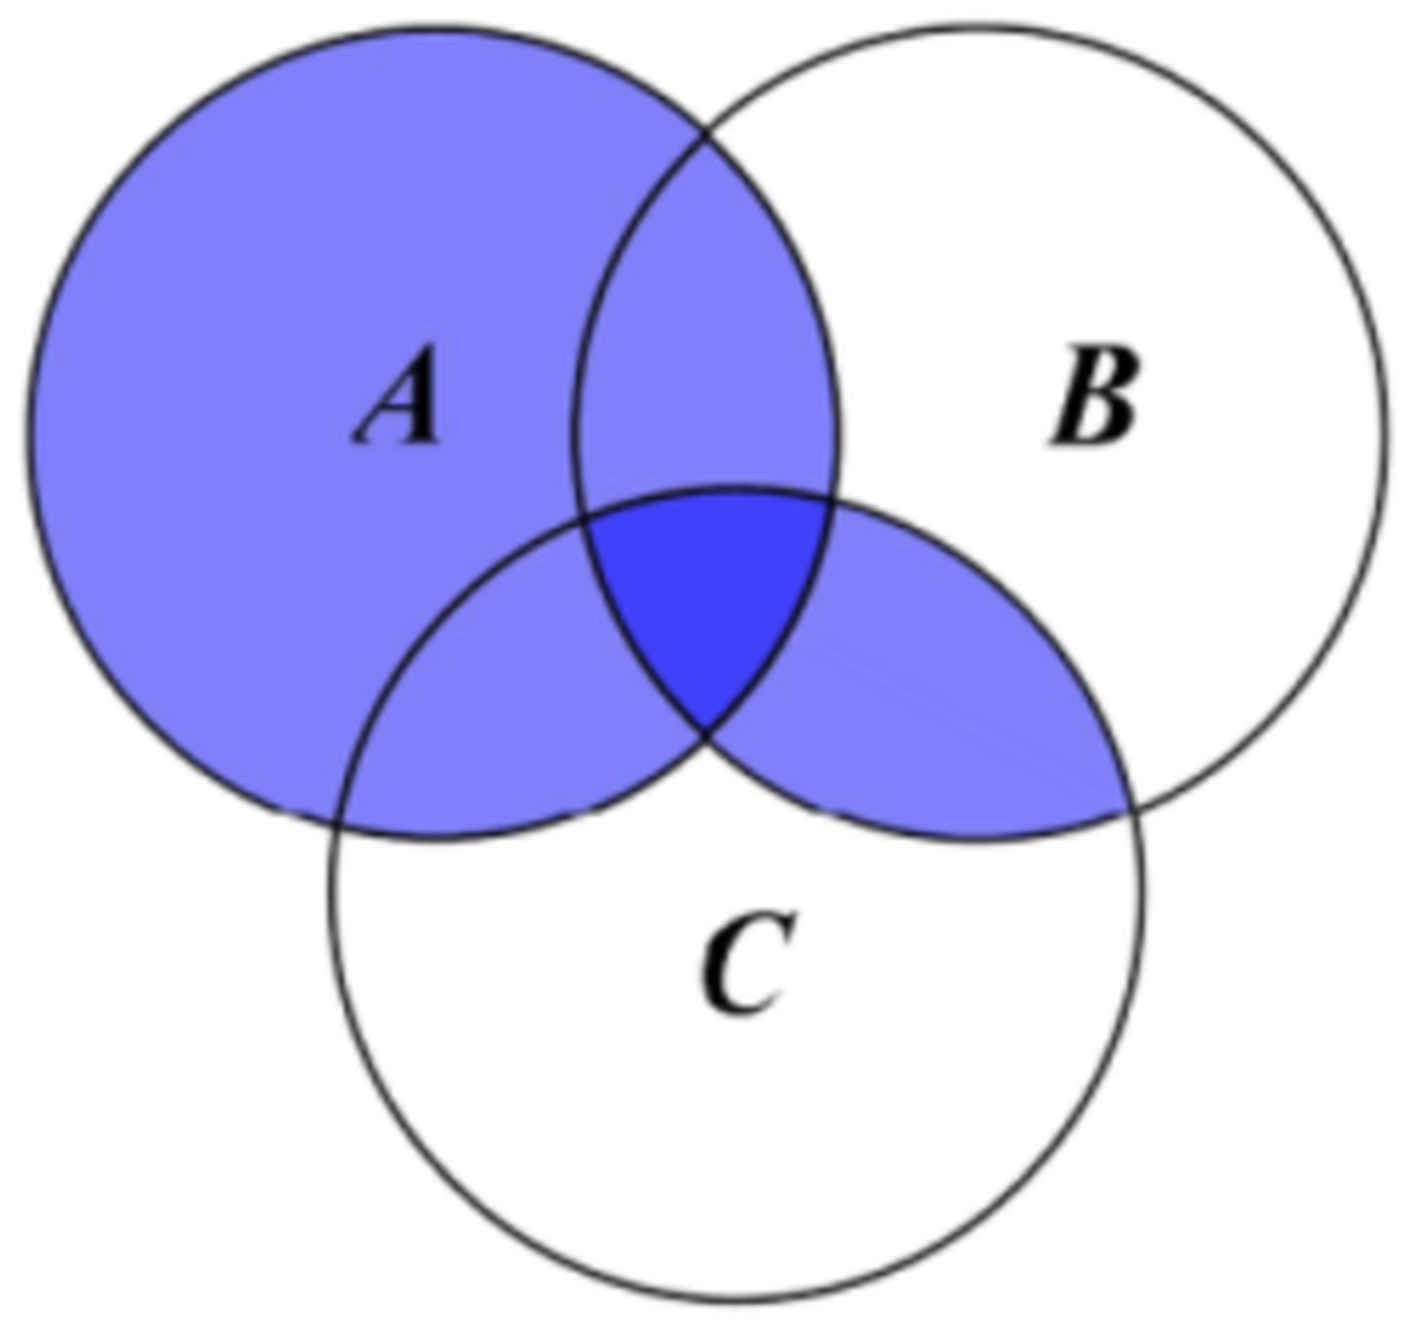
\includegraphics[width=0.30\textwidth]{figures/venn_A_union_BC.png}
\end{center}

\keepwithprev
A. $(A\cup C)\cap(B\cup C)$\qquad\qquad B. $(A\cup B)\cap(A\cup C)$

C. $(A\cup B)\cap(B\cup C)$\qquad\qquad D. $(A\cup B)\cap C$

\ans{$B$}

\ifanswer
\solbegin
\step{图中阴影部分表示元素满足是 $A$ 中的元素，或者是 $B$ 与 $C$ 的公共元素，}
\step{故可以表示为 $A\cup(B\cap C)$，也可以表示为 $(A\cup B)\cap(A\cup C)$.
故选 $B$.}
\solend

\fi

\item 设集合 $M=\left\{x\mid m\leqslant x\leqslant m+\dfrac34\right\}$，
$N=\left\{x\mid n-\dfrac13\leqslant x\leqslant n\right\}$，且 $M$、$N$ 都是集合
$\{x\mid0\leqslant x\leqslant1\}$ 的子集，如果把 $b-a$ 叫做集合
$\{x\mid a\leqslant x\leqslant b\}$ 的“长度”，那么集合 $M\cap N$ 的“长度”的
最小值是\mbox{（\quad）}

\keepwithprev
A. $\dfrac23$\qquad B. $\dfrac1{12}$\qquad C. $\dfrac13$\qquad D. $\dfrac5{12}$

\ans{$B$}

\ifanswer
\solbegin
\step{$M$ 的长度为 $\dfrac34$，$N$ 的长度为 $\dfrac13$，}
\step{当集合 $M\cap N$ 的长度的最小值时，$M$ 与 $N$ 应分别在区间 $[0,1]$ 的左右两端，}
\step{故 $M\cap N$ 的长度的最小值是 $\dfrac34+\dfrac13-1=\dfrac1{12}$，故选 $B$.}
\solend

\fi

\item 定义集合运算 $A-B=\{x\mid x\in A\text{ 且 }x\notin B\}$ 称为集合 $A$ 与集合 $B$ 的
差集；定义集合运算 $A\Delta B=(A-B)\cup(B-A)$ 称为集合 $A$ 与集合 $B$ 的对称差，
有以下 $4$ 个等式：① $A\Delta B=B\Delta A$；② $(A\Delta B)\Delta C=A\Delta(B\Delta C)$；
③ $A\cap(B\Delta C)=(A\cap B)\Delta(A\cap C)$；
④ $A\cup(B\Delta C)=(A\cup B)\Delta(A\cup C)$，
则 $4$ 个等式中恒成立的是\mbox{（\quad）}

\keepwithprev
A. ①②\qquad B. ①②③\qquad C. ①②④\qquad D. ①②③④

\ans{$B$}

\ifanswer
\solbegin
\step{对于①，由 $B\Delta A=(B-A)\cup(A-B)=(A-B)\cup(B-A)=A\Delta B$，
所以①正确；}
\step{对于②，由 $A-B=\{x\mid x\in A\text{ 且 }x\notin B\}
=\{x\mid x\in A,x\notin(A\cap B)\}=A-(A\cap B)$，}
\step{同理可得 $B-A=B-(A\cap B)$，}
\step{则 $A\Delta B=(A-B)\cup(B-A)=(A\cup B)-(A\cap B)$，}
\step{所以 $(A\Delta B)\Delta C=(A\Delta B)\cup C-(A\Delta B)\cap C$，}
\step{所以表示的集合为图（1）中阴影部分所表示的集合，如图所示，}
\step{同理 $A\Delta(B\Delta C)=A\cup(B\Delta C)-A\cap(B\Delta C)$，
也表示图（1）中阴影部分所表示的集合，}
\step{所以 $(A\Delta B)\Delta C=A\Delta(B\Delta C)$，所以②正确；}

\begin{center}
% 图取原卷截图、4× LANCZOS 放大（原卷印在下一页顶部，共三幅三圆韦恩图：
% 图（1）一幅、图（2）左右两幅，图（2）两幅下方各有一行式子标注）。
% 图只在【解析】里出现，故放进 \ifanswer 块，试卷版不排。
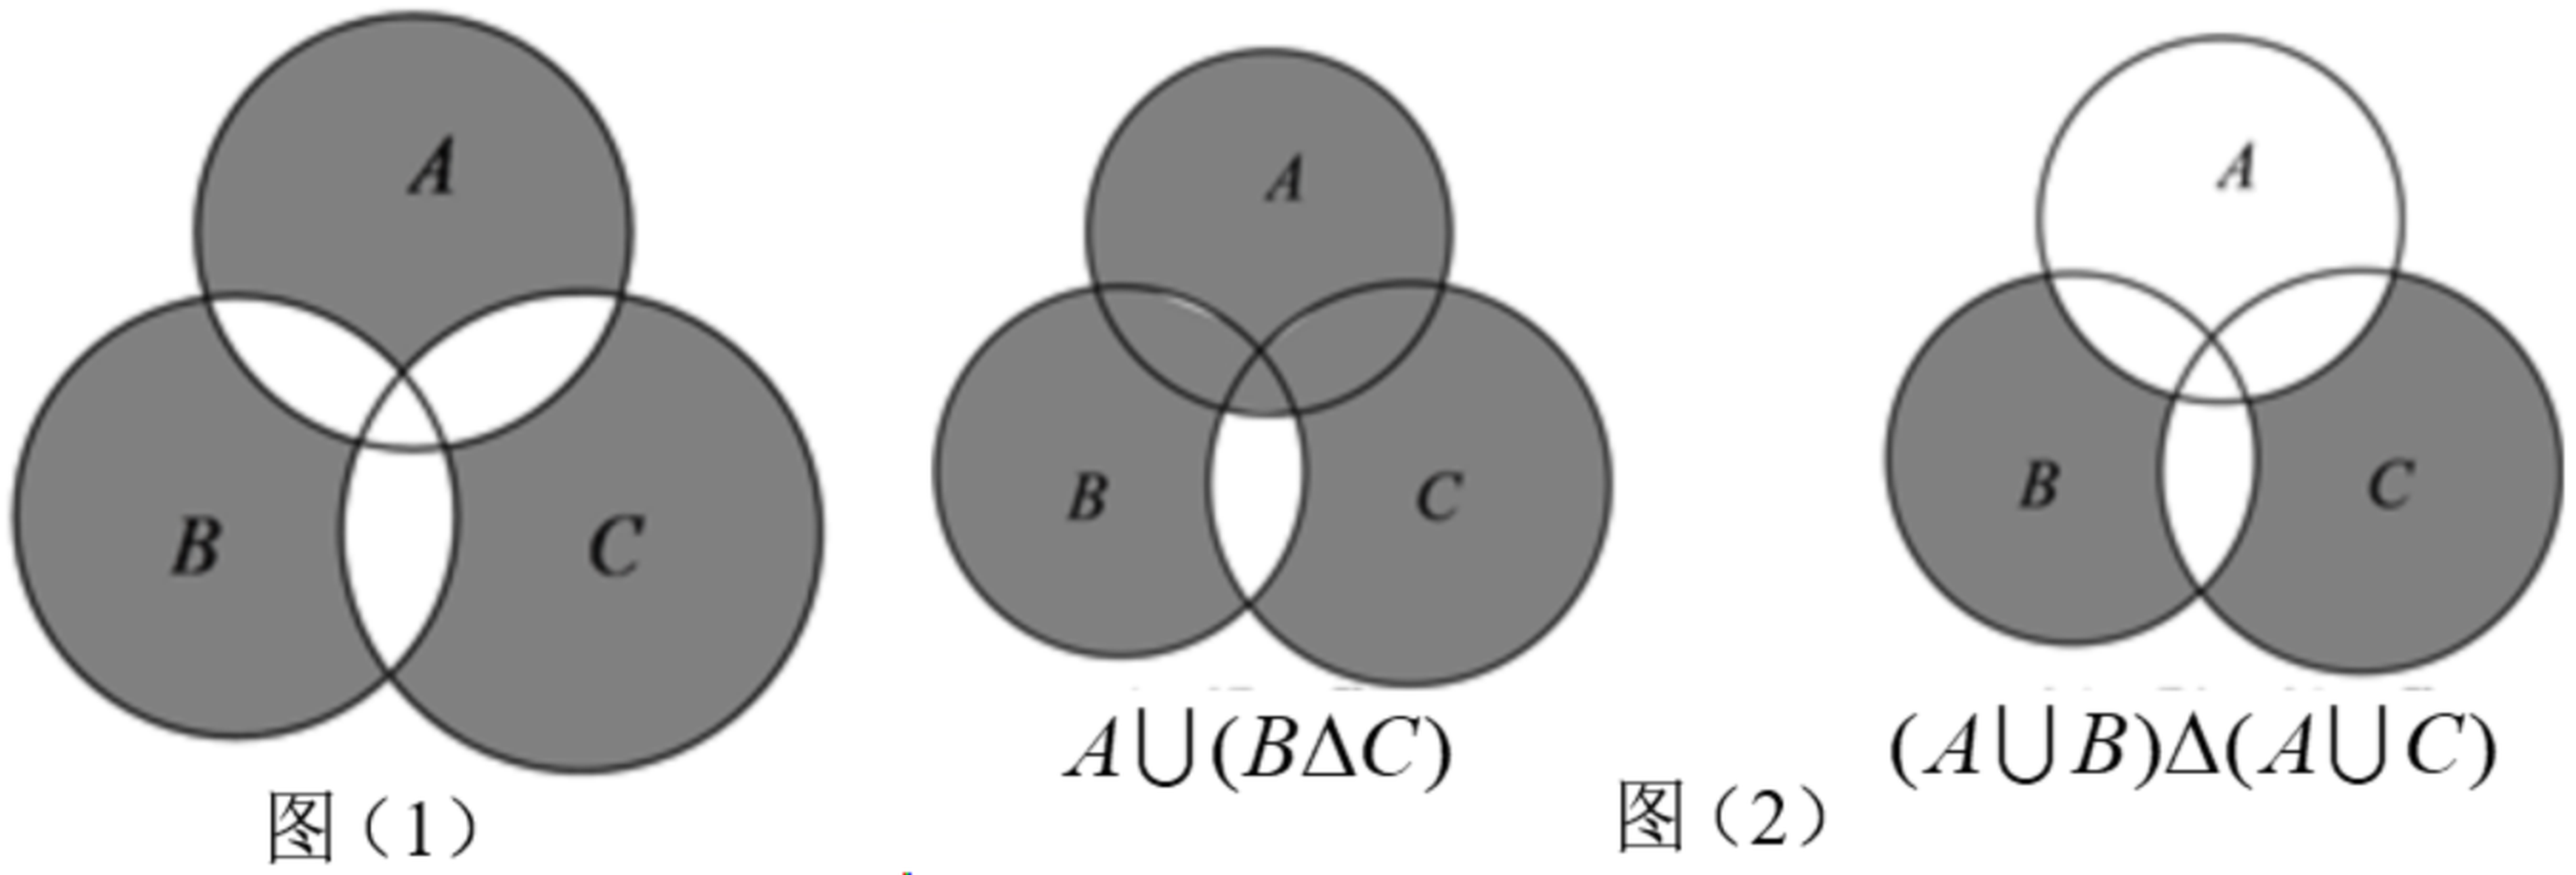
\includegraphics[width=0.86\textwidth]{figures/venn_symdiff3.png}
\end{center}

\step{对于③，由 $A\cap(B\Delta C)=A\cap(B\cup C-B\cap C)
=A\cap(B\cup C)-A\cap(B\cap C)$}
\step{$=(A\cap B)\cup(A\cap C)-(A\cap B)\cap(A\cap C)=(A\cap B)\Delta(A\cap C)$，
所以③正确；}
\step{对于④，如图（2）所示，$A\cup(B\Delta C)\neq(A\cup B)\Delta(A\cup C)$，
所以④错误.}
\step{故选 $B$.}
\solend

\fi

\end{enumerate}

\bigsec{三、解答题}

\begin{enumerate}
\setcounter{enumi}{16}

\item 已知集合 $M=\{x\mid a-1\leqslant x\leqslant2a+3\}$，$P=\{x\mid-2<x\leqslant4\}$，
全集 $U=\R$.

\begin{enumerate}[label=(\arabic*)]
\item 当 $a=2$ 时，求 $M\cap P$；
\item 若 $x\in P$ 是 $x\in M$ 的必要不充分条件，求实数 $a$ 的取值范围.
\end{enumerate}

\ifanswer
\solbegin
\stepm{(1)}{当 $a=2$ 时，集合 $M=\{x\mid1\leqslant x\leqslant7\}$，}
\step{所以 $M\cap P=\{x\mid1\leqslant x\leqslant4\}$；}
\stepm{(2)}{因为 $x\in P$ 是 $x\in M$ 的必要不充分条件，所以 $M\subset P$，}
\step{当 $M=\varnothing$ 时，$a-1>2a+3$，解得 $a<-4$，}
\step{当 $M\neq\varnothing$ 时，则
$\begin{cases}a-1\leqslant2a+3\\ a-1>-2\\ 2a+3\leqslant4\end{cases}$，
解得 $-1<a\leqslant\dfrac12$，}
\step{综上所述，实数 $a$ 的取值范围为
$(-\infty,-4)\cup\left(-1,\dfrac12\right]$.}
\solend

\fi

\ansspace[6]

\item 一辆汽车在某段路程中的行驶速度与时间的关系如图：

\begin{center}
% 图取原卷截图、4× LANCZOS 放大（速度—时间图：纵轴 $v/(\mathrm{km/h})$、
% 横轴 $t(\mathrm{h})$，$t\in[0,1]$、$[1,2]$、$[2,3]$ 三段矩形条高 50、80、90）。
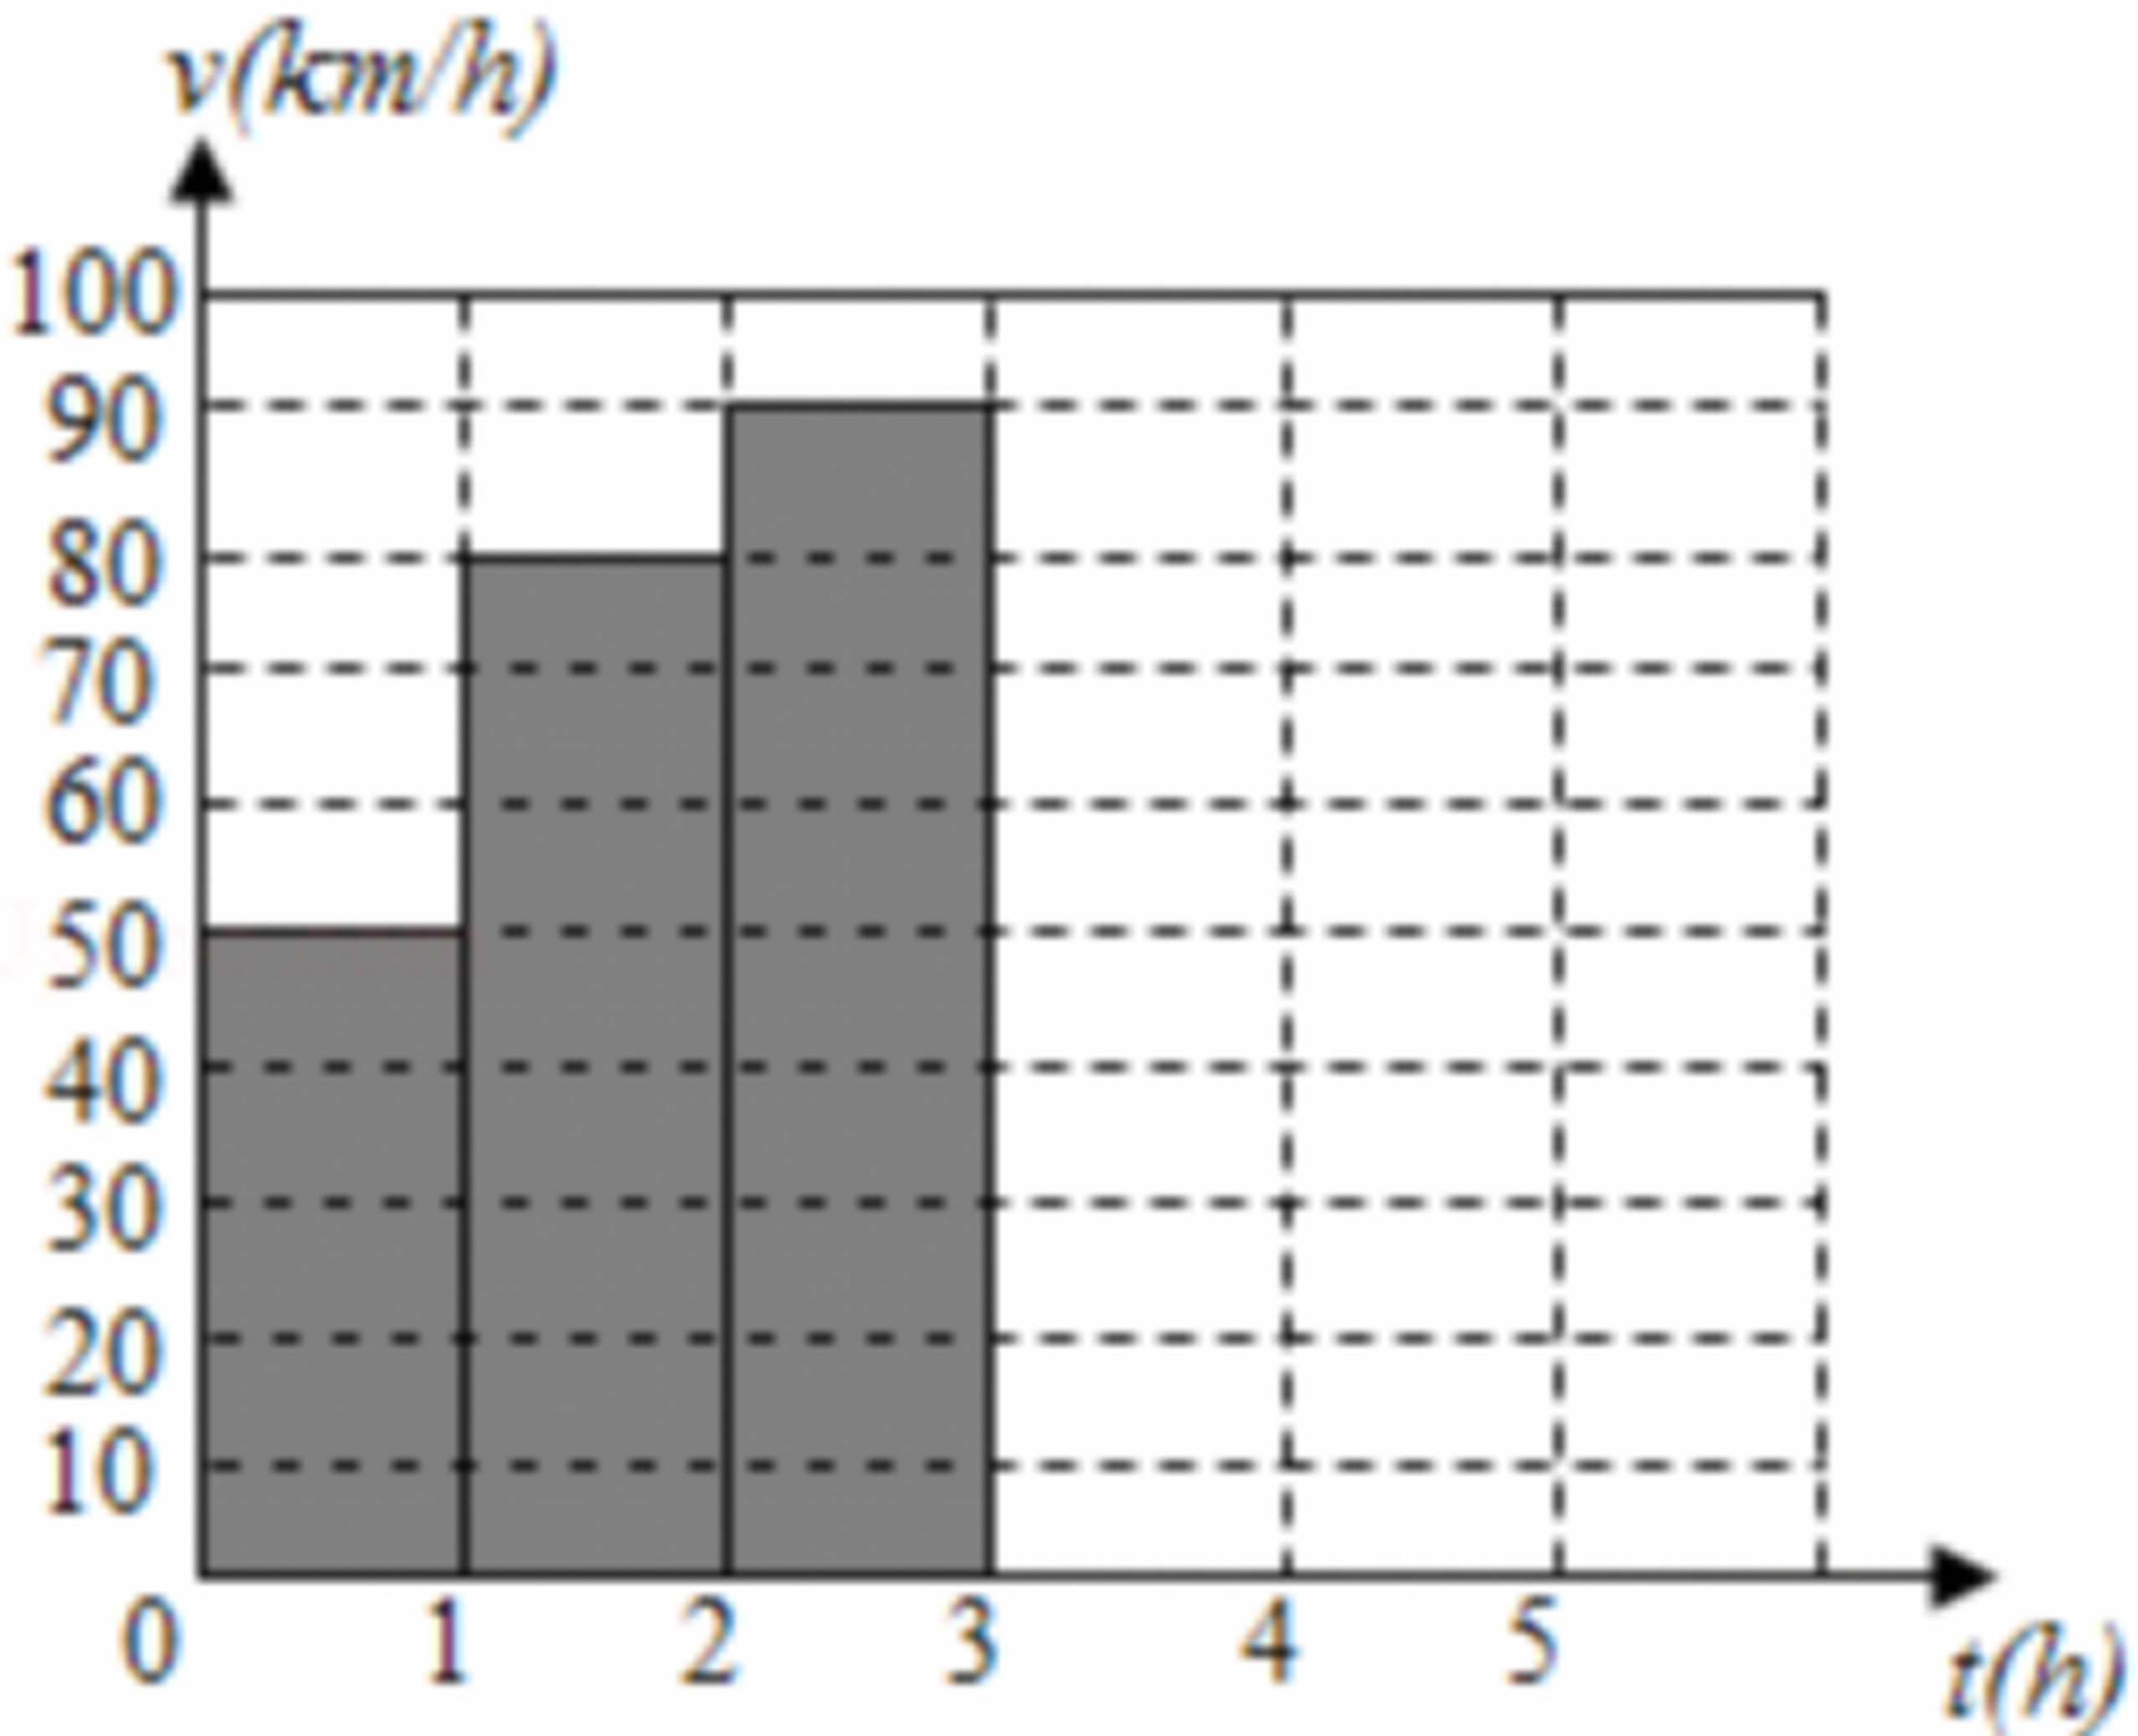
\includegraphics[width=0.52\textwidth]{figures/speed_time_bars.png}
\end{center}

\begin{enumerate}[label=(\arabic*)]
\item 求图中阴影部分的面积，并说明所求面积的实际意义；
\item 假设这辆汽车的里程表在汽车行驶这段路程前的读数为 $2004\,\mathrm{km}$，
试将汽车行驶这段路程时汽车里程表读数 $S$ 表示为时间 $t$ 的函数，
并求出当汽车里程表读数为 $2094\,\mathrm{km}$ 时，汽车行驶了多少时间？
\end{enumerate}

\ifanswer
\solbegin
\stepm{(1)}{由一辆汽车在某段路程中的行驶速度与时间的关系图，}
\step{得阴影部分的面积为 $50\times1+80\times1+90\times1=220$，}
\step{阴影部分的面积表示汽车在 $3$ 小时内行驶的路程为 $220\,\mathrm{km}$.}
\stepm{(2)}{$S=\begin{cases}
50t+2004,&0\leqslant t<1\\
80(t-1)+2054,&1\leqslant t<2\\
90(t-2)+2134,&2\leqslant t\leqslant3
\end{cases}$}
\step{令 $80(t-1)+2054=2094$，解得 $t=1.5$，所以汽车行驶 $1.5$ 小时.}
\solend

\fi

\ansspace[6]

\item 已知集合 $A=\{x\mid x<-2\text{ 或 }x\geqslant3\}$，$U=\R$.

\begin{enumerate}[label=(\arabic*)]
\item 求 $\overline{A}$；
\item 若 $B=\{x\mid mx-1>0\}$，当 $B\sub A$ 时，求实数 $m$ 的取值范围；
\item 若 $B=\{x\mid2m-6\leqslant x\leqslant m+4\}$，当 $B\cap\overline{A}=\varnothing$ 时，
求实数 $m$ 的取值范围.
\end{enumerate}

\ifanswer
\solbegin
\stepm{(1)}{因为集合 $A=\{x\mid x<-2\text{ 或 }x\geqslant3\}$，$U=\R$，
所以 $\overline{A}=\{x\mid-2\leqslant x<3\}$；}
\stepm{(2)}{当 $m=0$ 时，$B=\varnothing$，符合题意，}
\step{当 $m>0$ 时，$B=\left\{x\mid x>\dfrac1m\right\}$，则 $\dfrac1m\geqslant3$，
解得 $0<m\leqslant\dfrac13$，}
\step{当 $m<0$ 时，$B=\left\{x\mid x<\dfrac1m\right\}$，则 $\dfrac1m\leqslant-2$，
解得 $-\dfrac12\leqslant m<0$，}
\step{综上所述，实数 $m$ 的取值范围 $\left[-\dfrac12,\dfrac13\right]$；}
\stepm{(3)}{由题意得 $B=\{x\mid2m-6\leqslant x\leqslant m+4\}$，
$\overline{A}=\{x\mid-2\leqslant x<3\}$，且 $B\cap\overline{A}=\varnothing$，}
\step{当 $B=\varnothing$ 时，$2m-6>m+4$，解得 $m>10$，}
\step{当 $B\neq\varnothing$ 时，则 $\begin{cases}2m-6\leqslant m+4\\ m+4<-2\end{cases}$
或 $\begin{cases}2m-6\leqslant m+4\\ 2m-6\geqslant3\end{cases}$，}
\step{解得 $m<-6$ 或 $\dfrac92\leqslant m\leqslant10$，}
\step{综上所述，实数 $m$ 的取值范围为
$(-\infty,-6)\cup\left[\dfrac92,+\infty\right)$.}
\solend

\fi

\ansspace[8]

\item 在等腰梯形 $ABCD$ 中，$AB=DC=5$，$AD=4$，$BC=10$. 点 $E$ 在下底边 $BC$ 上.
点 $F$ 在腰 $AB$ 上.

\begin{center}
% 图取原卷截图、4× LANCZOS 放大（等腰梯形 $ABCD$ 与线段 $FE$，无辅助线）。
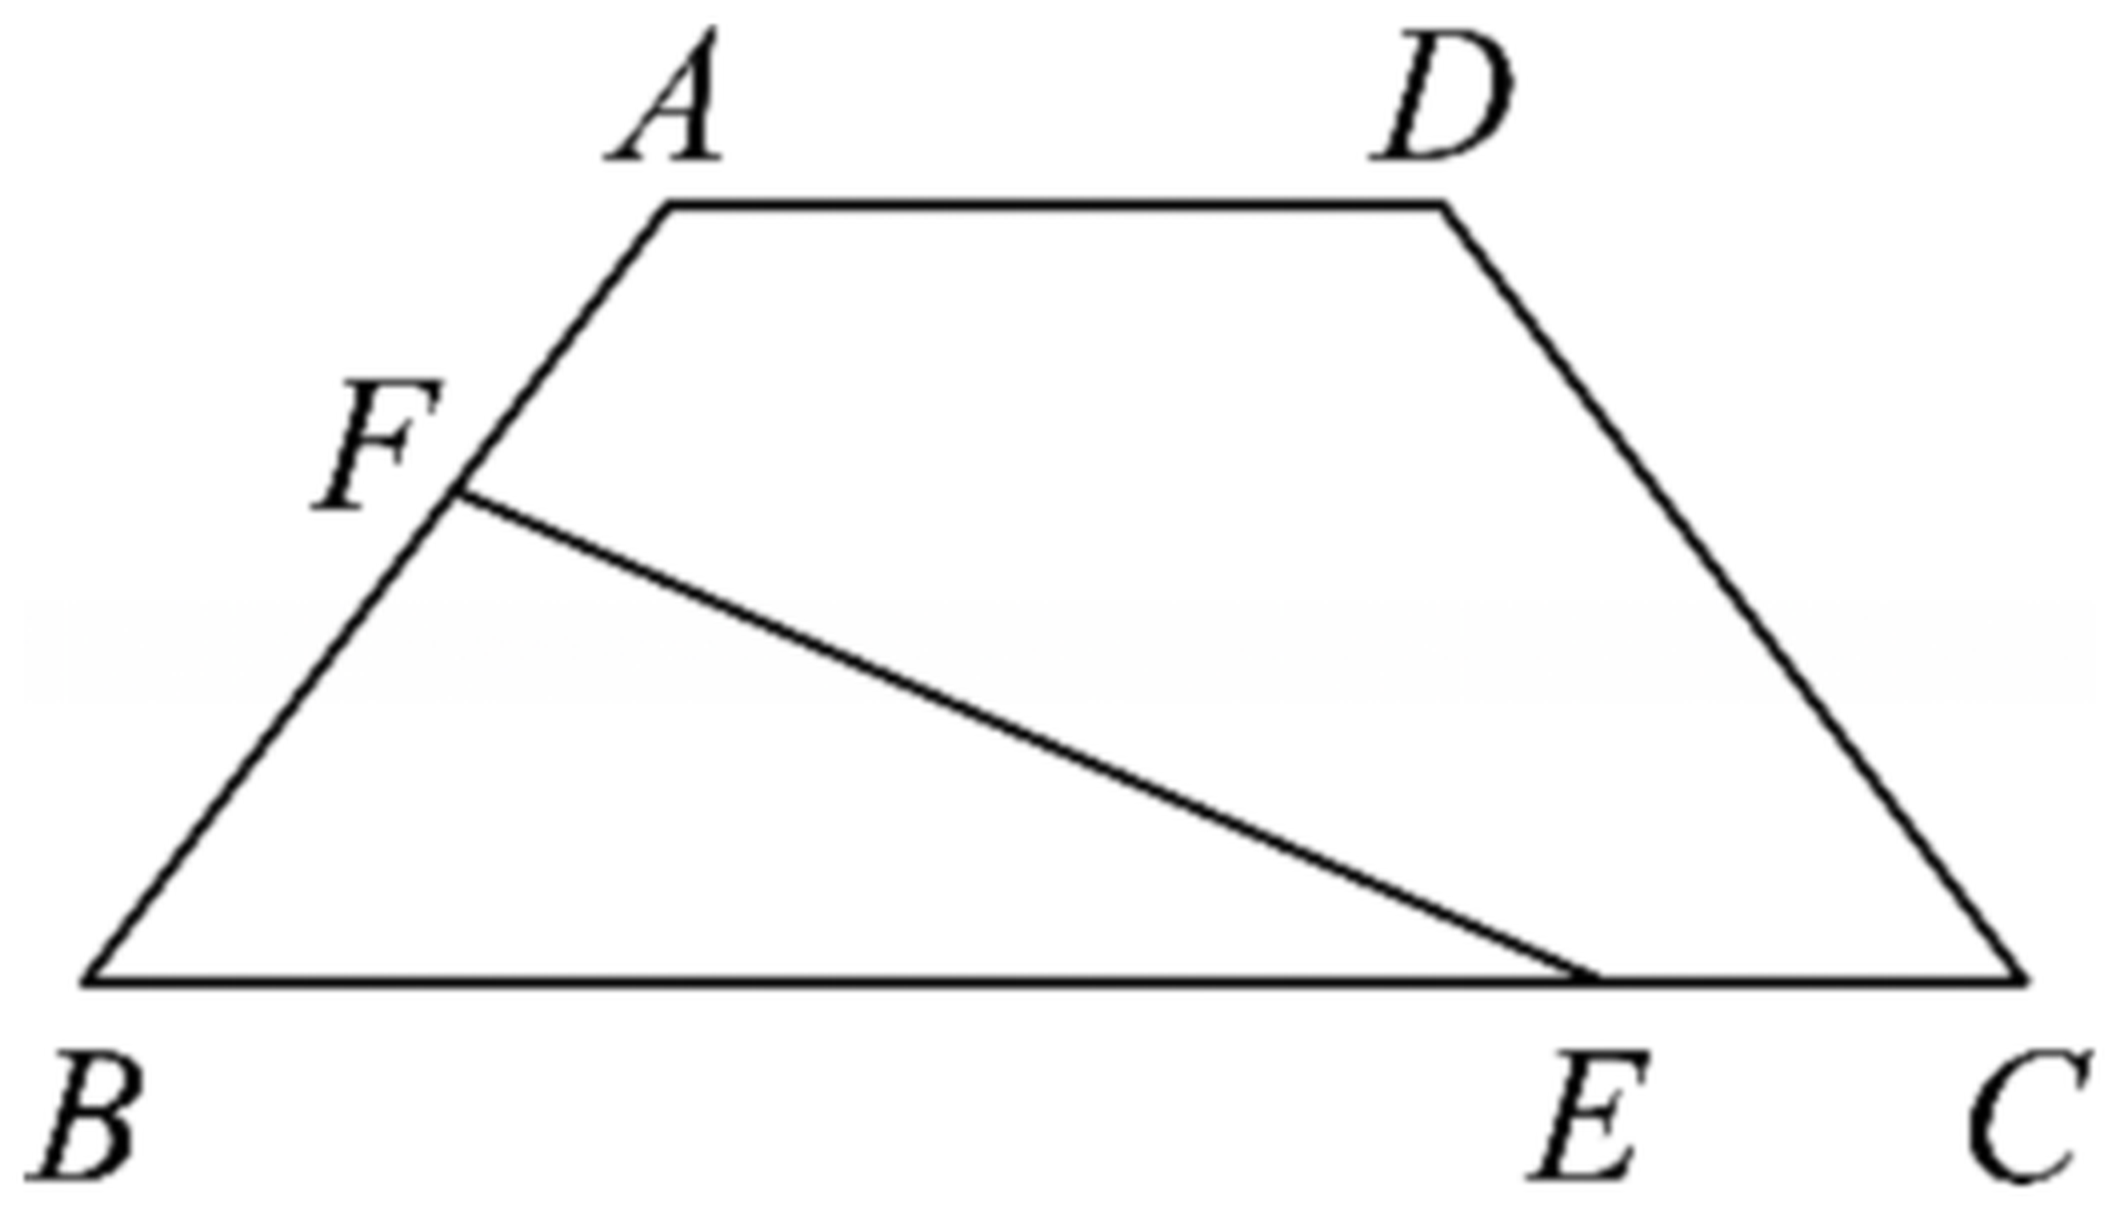
\includegraphics[width=0.46\textwidth]{figures/trapezoid_EF.png}
\end{center}

\begin{enumerate}[label=(\arabic*)]
\item 若 $EF$ 平分等腰梯形 $ABCD$ 的周长，设 $BE$ 长为 $x$，试用含 $x$ 的代数式表示
$\triangle BEF$ 的面积；
\item 是否存在线段 $EF$ 将等腰梯形 $ABCD$ 的周长和面积同时平分？若存在，求出此时 $BE$
的长；若不存在，请说明理由；
\item 是否存在线段 $EF$ 将等腰梯形 $ABCD$ 的周长和面积同时分成 $1:2$ 的两部分？
若存在，求此时 $BE$ 的长；若不存在，请说明理由.
\end{enumerate}

\ifanswer
\solbegin
\stepm{(1)}{过 $A$ 作 $AK\perp BC$ 交 $BC$ 于点 $K$，过 $F$ 作 $FG\perp BC$ 交 $BC$ 于点
$G$，}

\begin{center}
% 图取原卷截图、4× LANCZOS 放大（同梯形，多出虚线 $FG\perp BC$ 与 $AK\perp BC$
% 及两处直角符号；图只在【解析】里出现，故放进 \ifanswer 块）。
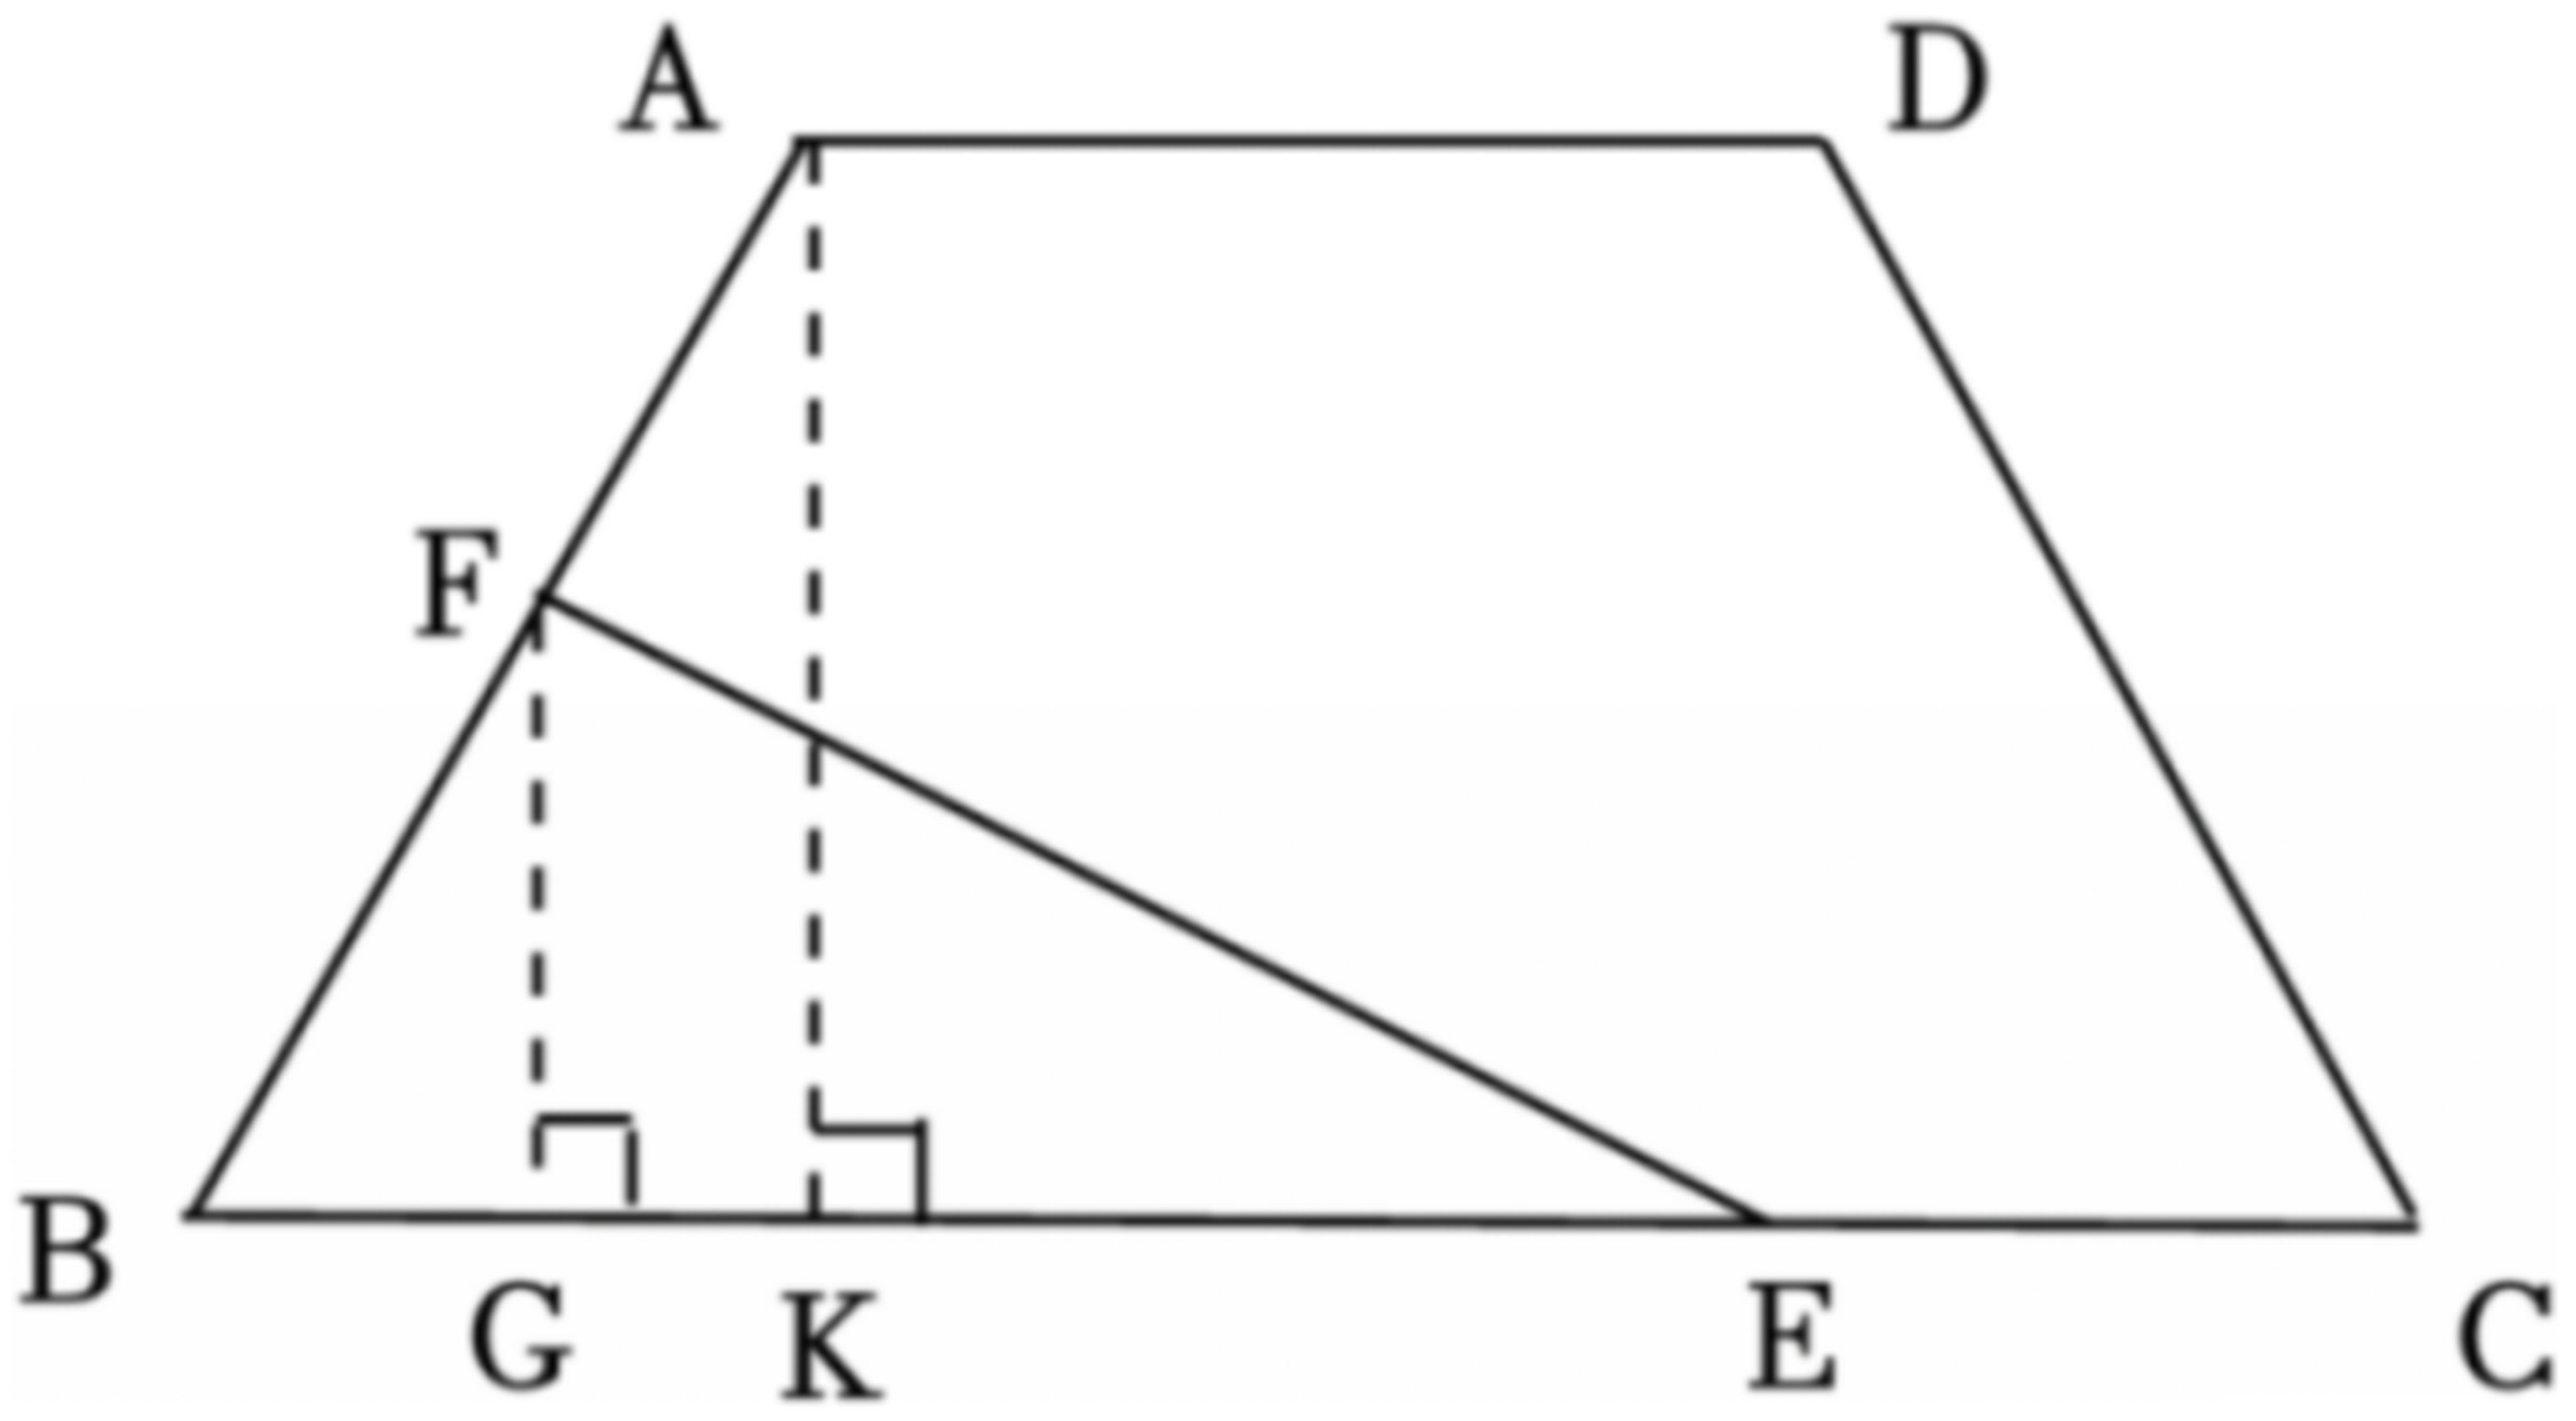
\includegraphics[width=0.62\textwidth]{figures/trapezoid_EF_aux.png}
\end{center}

\step{所以 $BK=\dfrac12\times(BC-AD)=\dfrac12\times(10-4)=3$，}
\step{$AK=\sqrt{AB^2-BK^2}=\sqrt{5^2-3^2}=4$，}
\step{由题意得，梯形 $ABCD$ 周长为 $24$，高为 $4$，面积为 $28$，}
\step{因为 $EF$ 平分等腰梯形 $ABCD$ 的周长，设 $BE$ 长为 $x$，则 $BF=12-x$，}
\step{由 $\begin{cases}0\leqslant12-x\leqslant5\\ 0\leqslant x\leqslant10\end{cases}$，
解得 $7\leqslant x\leqslant10$，}
\step{由题意得 $\triangle BFG\backsim\triangle BAK$，所以 $\dfrac{FG}{AK}=\dfrac{BF}{BA}$，
即 $\dfrac{FG}4=\dfrac{12-x}5$，}
\step{解得 $FG=\dfrac45(12-x)$，}
\step{所以 $S_{\triangle BEF}=\dfrac12BE\cdot FG
=-\dfrac25x^2+\dfrac{24}5x$（$7\leqslant x\leqslant10$）；}
\stepm{(2)}{存在，由 (1) 得 $-\dfrac25x^2+\dfrac{24}5x=\dfrac{28}2$，$x\in[7,10]$，}
\step{即 $x^2-12x+35=0$，解得 $x=7$ 或 $x=5$（舍去），}
\step{所以存在线段 $EF$ 将等腰梯形 $ABCD$ 的周长和面积同时平分，此时 $BE=7$；}
\stepm{(3)}{不存在，}
\step{情况一：$\triangle BEF$ 的面积$:$多边形 $AFECD$ 的面积 $=1:2$，
$(BE+BF):(AF+AD+DC+CE)=1:2$，}
\step{梯形周长的 $\dfrac13$ 是 $\dfrac{24}3=8$，面积的 $\dfrac13$ 是 $\dfrac{28}3$，}
\step{又因为 $BE=x$，所以 $BF=8-x$，}
\step{又因为 $\dfrac{FG}{AK}=\dfrac{BF}{BA}$，即 $\dfrac{FG}4=\dfrac{8-x}5$，
所以 $FG=\dfrac{32-4x}5$，}
\step{所以 $S_{\triangle BEF}=\dfrac12BE\times FG=-\dfrac25x^2+\dfrac{16}5x$，
所以 $\dfrac{28}3=-\dfrac25x^2+\dfrac{16}5x$，}
\step{整理得 $-3x^2+24x-70=0$，此时 $\Delta<0$，无解，故不存在；}
\step{情况二：$\triangle BEF$ 的面积$:$多边形 $AFECD$ 的面积 $=2:1$，
$(BE+BF):(AF+AD+DC+CE)=2:1$，}
\step{梯形周长的 $\dfrac13$ 为 $\dfrac{24}3=8$，面积的 $\dfrac13$ 为 $\dfrac{28}3$，
又 $BE=x$，所以 $BF=16-x$，}
\step{又 $\dfrac{FG}{AK}=\dfrac{BF}{BA}$，即 $\dfrac{FG}4=\dfrac{16-x}5$，
所以 $FG=\dfrac{64-4x}5$，}
\step{所以 $S_{\triangle BEF}=\dfrac12BE\times FG=-\dfrac25x^2+\dfrac{32}5x$，}
\step{所以 $\dfrac{28}3\times2=-\dfrac25x^2+\dfrac{32}5x$，
整理得 $-3x^2+48x-140=0$，}
\step{解得 $x=\dfrac{48+\sqrt{624}}6>10$，$x=\dfrac{48-\sqrt{624}}6<7$，
不符合题意，舍去，故不存在；}
\step{综上所述，不存在线段 $EF$ 将等腰梯形 $ABCD$ 的周长和面积同时分成 $1:2$ 的两部分.}
\solend

\fi

\ansspace[8]

\item 对集合 $\{1,2,\cdots,n\}$ 及其每一个非空子集 $A$，定义一个唯一确定的“交替和”
如下：将 $A$ 中的元素按照递减的次序排列，然后将第一个元素交替地减或加后继的元素所得的
结果，例如，子集 $\{1,2,4,6,9\}$ 的“交替和”是 $9-6+4-2+1=6$，子集 $\{5,6\}$ 的
“交替和”是 $6-5=1$，子集 $\{2\}$ 的交替和是 $2$；定义一个唯一确定的“交替积”如下：
将 $A$ 中的元素按照递减的次序排列，然后将第一个元素交替地除以或乘以后继的数所得的结果，
例如，集合 $\{1,2,4,6,9\}$ 的“交替积”是 $9\div6\times4\div2\times1=3$，
$\{5,6\}$ 的“交替积”是 $6\div5=1.2$，$\{2\}$ 的“交替积”是 $2$.

\begin{enumerate}[label=(\arabic*)]
\item 对于 $\{1,2,3,4,5,6,7,8,9\}$，求其所有子集的“交替和”的总和；
\item 对于 $\{1,2,\cdots,n\}$，求其所有子集的“交替和”的总和；
\item 对于 $\left\{n\mid\dfrac{495}{n+2}\in\N,n\in\Z\right\}$ 求其所有子集的
“交替积”的总和.
\end{enumerate}

\ifanswer
\solbegin
\stepm{(1)}{集合 $\{1,2,3,4,5,6,7,8,9\}$ 的子集中，除去 $\{9\}$ 外还有 $2^9-2$ 个
非空子集，}
\step{把这 $2^9-2$ 个非空子集两两组合后分别计算每一组中“交替和”之和，}
\step{组合原则是设 $A_i=\{9,a_1,a_2,\cdots\}$，$A_i^1=\{a_1,a_2,\cdots\}$，}
\step{集合 $A_i^1$ 的元素为集合 $A_i$ 中去掉 $9$ 的所有元素，把 $A_i$ 和 $A_i^1$
结合为一组，}
\step{显然，每组的“交替和”的和为 $9$，共有 $\dfrac{2^9-2}2$ 组，}
\step{所以，所有“交替和”之和应该为 $\dfrac{9(2^9-2)}2+9=2304$；}
\stepm{(2)}{集合 $\{1,2,\cdots,n\}$ 的子集中，除去 $\{n\}$ 外还有 $2^n-2$ 个非空子集，}
\step{把这 $2^n-2$ 个非空子集两两组合后分别计算每一组中“交替和”之和，}
\step{组合原则是设 $A_i=\{n,a_1,a_2,\cdots\}$，$A_i^1=\{a_1,a_2,\cdots\}$，}
\step{集合 $A_i^1$ 的元素为集合 $A_i$ 中去掉 $n$ 的所有元素，把 $A_i$ 和 $A_i^1$
结合为一组，}
\step{显然，每组的“交替和”的和为 $n$，共有 $\dfrac{2^n-2}2$ 组，}
% 注：下一行分子原卷印作花括号（其余同类处皆用圆括号），照抄未改，见文件头“原卷存疑”③。
\step{所以，所有“交替和”之和应该为 $\dfrac{n\{2^n-2\}}2+n=n\cdot2^{n-1}$；}
\stepm{(3)}{集合 $\left\{n\mid\dfrac{495}{n+2}\in\N,n\in\Z\right\}
=\{493,163,97,53,43,31,13,9,7,3,1,-1\}$，}
\step{其中除去 $\{-1\}$ 外还有 $2^{12}-2$ 个非空子集，}
% 注：下一行原卷把“把这”重复印了一次（“把这把这”），照抄未改，见文件头“原卷存疑”②。
\step{把这把这 $2^{12}-2$ 个非空子集两两组合后分别计算每一组中“交替积”之和，}
\step{组合原则是设 $A_j=\{-1,a_1,a_2,\cdots\}$，$A_j^1=\{a_1,a_2,\cdots\}$，}
\step{集合 $A_j^1$ 的元素为集合 $A_j$ 中去掉 $-1$ 的所有元素，把 $A_j$ 和 $A_j^1$
结合为一组，}
\step{显然，每组的“交替积”的和为 $0$，共有 $\dfrac{2^{12}-2}2$ 组，}
\step{所以，所有“交替积”之和应该为 $\dfrac{2^{12}-2}2\times0-1=-1$.}
\solend

\fi

\ansspace*[10]

\end{enumerate}

\end{document}
"
%
% 原始材料是微信公众号图文（公众号“魔都数学加油站”连载“27学年高一 30”，2026-09-23 发布，
% 原文标题“27学年高一30——2026-2027年上海市南洋模范中学高一上开学考”），
% 正文为 11 张 PNG 页。**同一篇里各页分辨率不一致**——第 2、3、9、10 页 4762×6735，
% 其余七页 2560×3620（已逐页打开确认，非下载缺档），取的是 mmbiz.qpic.cn/<hash>/0 的原图档。
% 原文本身就是一份**讲评版**：填空第 3—7 题下方印【答案】，第 8—12 题与其后各题印【解析】。
% 试题文字、答案与解析均照原卷录入，未改内容。卷面的粉色斜水印属水印，未录入。
%
% 卷首标题：原卷印作“2026-2027 年南洋模范中学高一上开学考”（公众号标题里的“上海市”
% 三字卷面标题行没有，本稿照卷面），年份区间按全稿惯例排 en dash，前缀照原卷保留“年”。
%
% 与原卷的排版差异（均已在 README“说明”中交代）：
%   ① 原文自**第 3 题**起（第 1、2 题未在该文中发布），故本稿题号亦自 3 起；
%   ② 原卷本就印有“一、填空题”“二、选择题”“三、解答题”三节标题，本稿照原卷分节，
%      只把标题改排成全稿统一的“大节标题”样式；
%   ③ 原卷填空第 3—7 题只印【答案】行、第 8 题起印【解析】（选择题答案写在解析末句
%      “故选 D／B”里），本稿统一改为试卷版隐去、答案版以 \ans{}／\ifanswer 块给出，
%      两版彻底分离；
%   ④ 子集符号原卷两种并用：第 7 题题干两处、第 19(2) 题作带下划线的 $\subseteq$，
%      第 17(2) 题解析作真包含的 $\subset$，本稿分别照录为 $\sub$ 与 $\subset$；
%   ⑤ 补集符号原卷一律作**上横线**（$\overline{A}$、$\overline{B}$），本稿照录；
%   ⑥ 原卷的实数集 R 一律作斜体（第 4 题、第 17 题与第 19 题题干的 $U=R$），
%      第 21(3) 题的自然数集与整数集作**粗体** $\mathbf{N}$、$\mathbf{Z}$，
%      本稿按全稿惯例统一写作 $\R$、$\N$、$\Z$；
%   ⑦ 原卷填空的横线约两个字宽，本稿按全稿惯例统一排 \blankline[4.4em]；
%   ⑧ 原卷未印副标题，本稿按全稿惯例补出副标题“集合与常用逻辑用语”——但本卷是开学考，
%      范围不止这一章：第 18 题是速度—时间图象题、第 20 题是等腰梯形的周长/面积平分问题，
%      副标题只标了主章节（见文末“高一30 专记”）；
%   ⑨ 第 13、14、18、20 题的图印在题干右侧、第 16 题的三幅图印在【解析】里的下一页顶部、
%      第 20 题【解析】另有一张带辅助线的图，本稿一律移至题干或解析之后；
%      图取原卷截图、4× LANCZOS 放大（见各 \includegraphics 前的注释）。
%
% 原卷存疑三处（均照抄原卷、未改，见源码中该处上方注释）：
%   ① 第 10 题【解析】验证“破晓集”时写的是 $\notin A$、$\in A$（如“$-2-2=-4\notin A$”），
%      但该处讨论的集合原题设里叫 $P$，同题②的“$x+y=2(k_1+k_2)\in A$”亦然——
%      本稿照抄未改（按文意应为 $P$）；
%   ② 第 21 题【解析】(3) 有“把这把这 $2^{12}-2$ 个非空子集”（“把这”重复印了一次）；
%   ③ 同题 (2) 的结论式分子原卷印作花括号 $\dfrac{n\{2^n-2\}}{2}$（其余同类处皆用圆括号）。

\documentclass[a4paper,11pt]{article}
\usepackage{common}

\begin{document}

\examtitlest[3]{2026--2027 年南洋模范中学高一上开学考}{集合与常用逻辑用语}

\bigsec{一、填空题}

\begin{enumerate}
\setcounter{enumi}{2}

\item 若集合 $A=\{x\mid x^2-2kx+7k=0\}$ 有且仅有三个真子集，则 $k$ 的取值范围是
\blankline[4.4em].

\ans{$(-\infty,0)\cup(7,+\infty)$}

\item “存在 $x\in\R$，使得 $x^2+2x+5=0$”的否定形式是 \blankline[4.4em].

\ans{对任何 $x\in\R$，都有 $x^2+2x+5\neq0$}

\item 下列命题中，$p$ 是 $q$ 的必要非充分条件的是 \blankline[4.4em].

① $p:x>2$ 且 $y>3$，$q:x+y>5$；

② $p$：四边形的四个角都相等，$q$：四边形是正方形.

\ans{②}

\item 若“条件 $\alpha:2\leqslant x\leqslant4$”是“条件 $\beta:3m-1\leqslant x\leqslant-m$”的
充分非必要条件，则 $m$ 的取值范围是 \blankline[4.4em].

\ans{$(-\infty,-4]$}

\item 满足 $\{1\}\sub M\sub\{1,2,4,5\}$ 的集合 $M$ 的个数为 \blankline[4.4em] 个.

\ans{$8$}

\item 已知集合 $A=\{1,2\}$，集合 $B=\{x\mid ax=6\}$，若 $A\cup B=A$，则 $a$ 的所有取值
构成的集合为 \blankline[4.4em].

\ifanswer
\solbegin
\step{因为 $A\cup B=A$，所以 $B\sub A$，}
\step{当 $a=0$ 时，$B=\varnothing$，满足 $B\sub A$；}
\step{当 $a\neq0$ 时，$B=\left\{\dfrac6a\right\}$，则 $\dfrac6a=1$ 或 $\dfrac6a=2$，
解得 $a=6$ 或 $a=3$，}
\step{综上所述，$a$ 的所有取值构成的集合为 $\{0,3,6\}$.}
\solend

\fi

\item 对于集合 $M$、$N$，定义 $M-N=\{x\mid x\in M\text{ 且 }x\notin N\}$，
$M\oplus N=(M-N)\cup(N-M)$，设 $A=\{y\mid y=|x|,x\in\R\}$，
$B=\{y\mid y=-(x-1)^2+2,x\in\R\}$，则 $A\oplus B=$ \blankline[4.4em].

\ifanswer
\solbegin
\step{由已知 $A=[0,+\infty)$，$B=(-\infty,2]$，}
\step{由于 $A-B=(2,+\infty)$，$B-A=(-\infty,0)$，}
\step{故 $A\oplus B=(A-B)\cup(B-A)=(-\infty,0)\cup(2,+\infty)$.}
\solend

\fi

\item 设 $P$ 为非空实数集满足：对任意给定的 $x$、$y\in P$（$x$、$y$ 可以相同），都有
$x+y\in P$，$x-y\in P$，$xy\in P$，则称 $P$ 为破晓集. 关于破晓集有下列结论：
①集合 $P=\{-2,-1,0,1,2\}$ 为破晓集；②集合 $P=\{x\mid x=2n,n\in\Z\}$ 为破晓集；
③若集合 $P_1$、$P_2$ 为破晓集，则 $P_1\cup P_2$ 为破晓集；④若集合 $P$ 为破晓集，
则一定有 $0\in P$；⑤若集合 $P_1$、$P_2$ 为破晓集，则 $P_1\cap P_2$ 为破晓集；
其中正确结论的序号是 \blankline[4.4em].

\ifanswer
\solbegin
% 注：以下几步原卷把该集合记作 $A$（题设里叫 $P$），照抄未改，见文件头“原卷存疑”①。
\step{对于①：$-2-2=-4\notin A$，故集合 $P=\{-2,-1,0,1,2\}$ 不为破晓集，故①错误；}
\step{②设 $x$、$y\in A$，则 $x=2k_1$，$y=2k_2$，且 $k_1$、$k_2\in\Z$，}
\step{故 $x+y=2(k_1+k_2)\in A$，$x-y=2(k_1-k_2)\in A$，$xy=4k_1k_2\in A$，}
\step{故集合 $P=\{x\mid x=2n,n\in\Z\}$ 为破晓集，故②正确；}
\step{③若集合 $P_1$、$P_2$ 为破晓集，设 $P_1=\{x\mid x=2k,k\in\Z\}$，
$P_2=\{x\mid x=3k,k\in\Z\}$，}
\step{但是 $P_1\cup P_2$ 不为破晓集，如 $x=2$，$y=3$ 时，$x+y=5$，
故 $5\notin(P_1\cup P_2)$，故③错误；}
\step{④若集合 $P$ 为破晓集，则取 $x=y$，$x-y=0\in A$，则一定有 $0\in P$，故④正确.}
\step{⑤正确；}
\step{故正确的是②④⑤.}
\solend

\fi

\item 已知集合 $M$ 的元素均为正整数，定义集合 $M$ 的“变项和”为：将 $M$ 中每个元素 $m$
都乘以 $(-1)^m$ 后再求和. 若集合 $A=\{n\mid1\leqslant n\leqslant10,n\in\N\}$，则集合 $A$
的所有非空子集的“变项和”的总和为 \blankline[4.4em].

\ifanswer
\solbegin
\step{$A$ 集合的所有非空子集中，每个元素出现的次数都是
$(2^{10}-1)-(2^9-1)=2^9$，}
\step{则集合 $A$ 的所有非空子集的“变项和”的总和为
$1\times(-1)^1\times2^9+2\times(-1)^2\times2^9+\cdots+10\times(-1)^{10}\times2^9$}
\step{$=(-1+2-3+4-\cdots-9+10)\times2^9=5\times2^9=2560$.}
\solend

\fi

\item 已知集合 $A=[t,t+1]\cup[t+4,t+9]$，$0\notin A$，存在正数 $\lambda$，使得对任意
$a\in A$，都有 $\dfrac\lambda a\in A$，则 $t$ 的值是 \blankline[4.4em].

\ifanswer
\solbegin
\step{当 $t>0$ 时，当 $a\in[t,t+1]$ 时，$\dfrac\lambda a\in[t+4,t+9]$，}
\step{当 $a\in[t+4,t+9]$ 时，$\dfrac\lambda a\in[t,t+1]$，}
\step{即当 $a=t$ 时，$\dfrac\lambda a\leqslant t+9$；当 $a=t+9$ 时，
$\dfrac\lambda a\geqslant t$，即 $\lambda=t(t+9)$；}
\step{当 $a=t+1$ 时，$\dfrac\lambda a\geqslant t+4$，当 $a=t+4$ 时，
$\dfrac\lambda a\leqslant t+1$，即 $\lambda=(t+1)(t+4)$，}
\step{所以 $t(t+9)=(t+1)(t+4)$，解得 $t=1$.}
\step{当 $t+1<0<t+4$ 时，当 $a\in[t,t+1]$ 时，$\dfrac\lambda a\in[t,t+1]$.}
\step{当 $a\in[t+4,t+9]$ 时，则 $\dfrac\lambda a\in[t+4,t+9]$，}
\step{即当 $a=t$ 时，$\dfrac\lambda a\leqslant t+1$，当 $a=t+1$ 时，
$\dfrac\lambda a\geqslant t$，即 $\lambda=t(t+1)$，}
\step{即当 $a=t+4$ 时，$\dfrac\lambda a\leqslant t+9$，当 $a=t+9$ 时，
$\dfrac\lambda a\geqslant t+4$，即 $\lambda=(t+4)(t+9)$，}
\step{所以 $t(t+1)=(t+4)(t+9)$，解得 $t=-3$.}
\step{当 $t+9<0$ 时，同理可得无解.}
\step{综上，$t$ 的值为 $1$ 或 $-3$.}
\solend

\fi

\end{enumerate}

\bigsec{二、选择题}

\begin{enumerate}
\setcounter{enumi}{12}

% 这道题是“题干 + 图 + 选项”约 6cm 的一整块，页末放不下就会被拆开（切页审计的 A 类），
% 故在题前先量一次页高：不够就把整道题干连图带选项一起挪到次页。
\needvspace{6.5cm}
\item 设 $U=\{1,2,3,4,5\}$，$A$、$B$ 都是 $U$ 的子集，且 $A\cap B=\{5\}$，
$\overline{A}\cap B=\{4\}$，$\overline{A}\cap\overline{B}=\{1,2\}$，
则以下四个判断中正确的是\mbox{（\quad）}

\begin{center}
% 图取原卷截图、4× LANCZOS 放大（原卷把图印在题干右侧，本稿移至此处，见文件头⑨）。
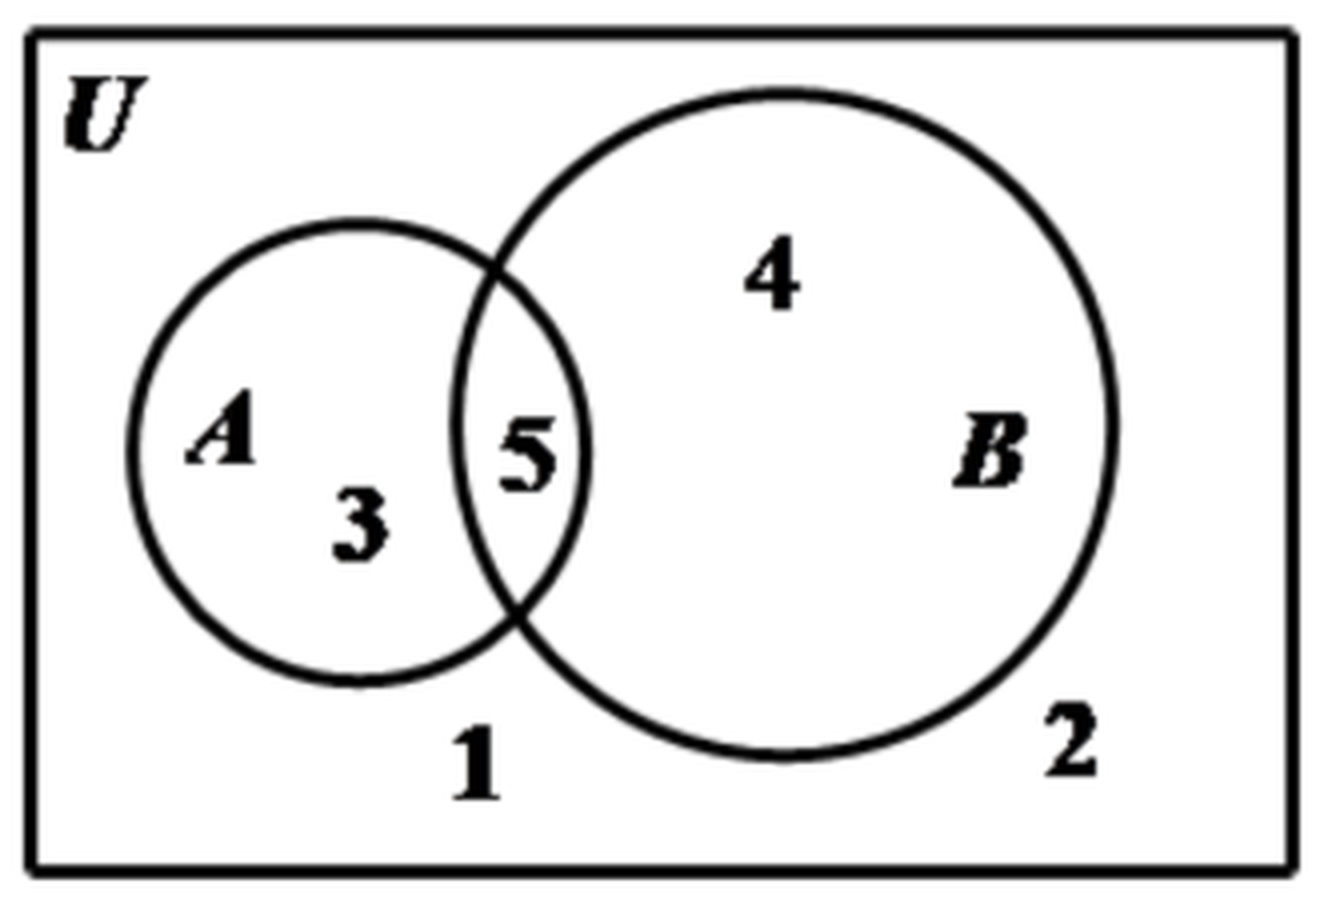
\includegraphics[width=0.28\textwidth]{figures/venn_U5_AB.png}
\end{center}

\keepwithprev
A. $3\notin A$ 且 $3\notin B$\qquad\qquad B. $3\in A$ 且 $3\in B$

C. $3\notin A$ 且 $3\in B$\qquad\qquad D. $3\in A$ 且 $3\notin B$

\ans{$D$}

\ifanswer
\solbegin
\step{画出韦恩图，得 $A=\{5,3\}$，$B=\{5,4\}$，}
\step{则 $3\in A$ 且 $3\notin B$. 故选 $D$.}
\solend

\fi

% 同第 13 题：整块（题干 + 图 + 选项）在答案版还要再挂【答案】【解析】，页末更易被拆开。
\needvspace{7.5cm}
\item 如图表示图形阴影部分的是\mbox{（\quad）}

\begin{center}
% 图取原卷截图、4× LANCZOS 放大（三圆 $A$、$B$、$C$，阴影为整个 $A$ 圆加 $B\cap C$）。
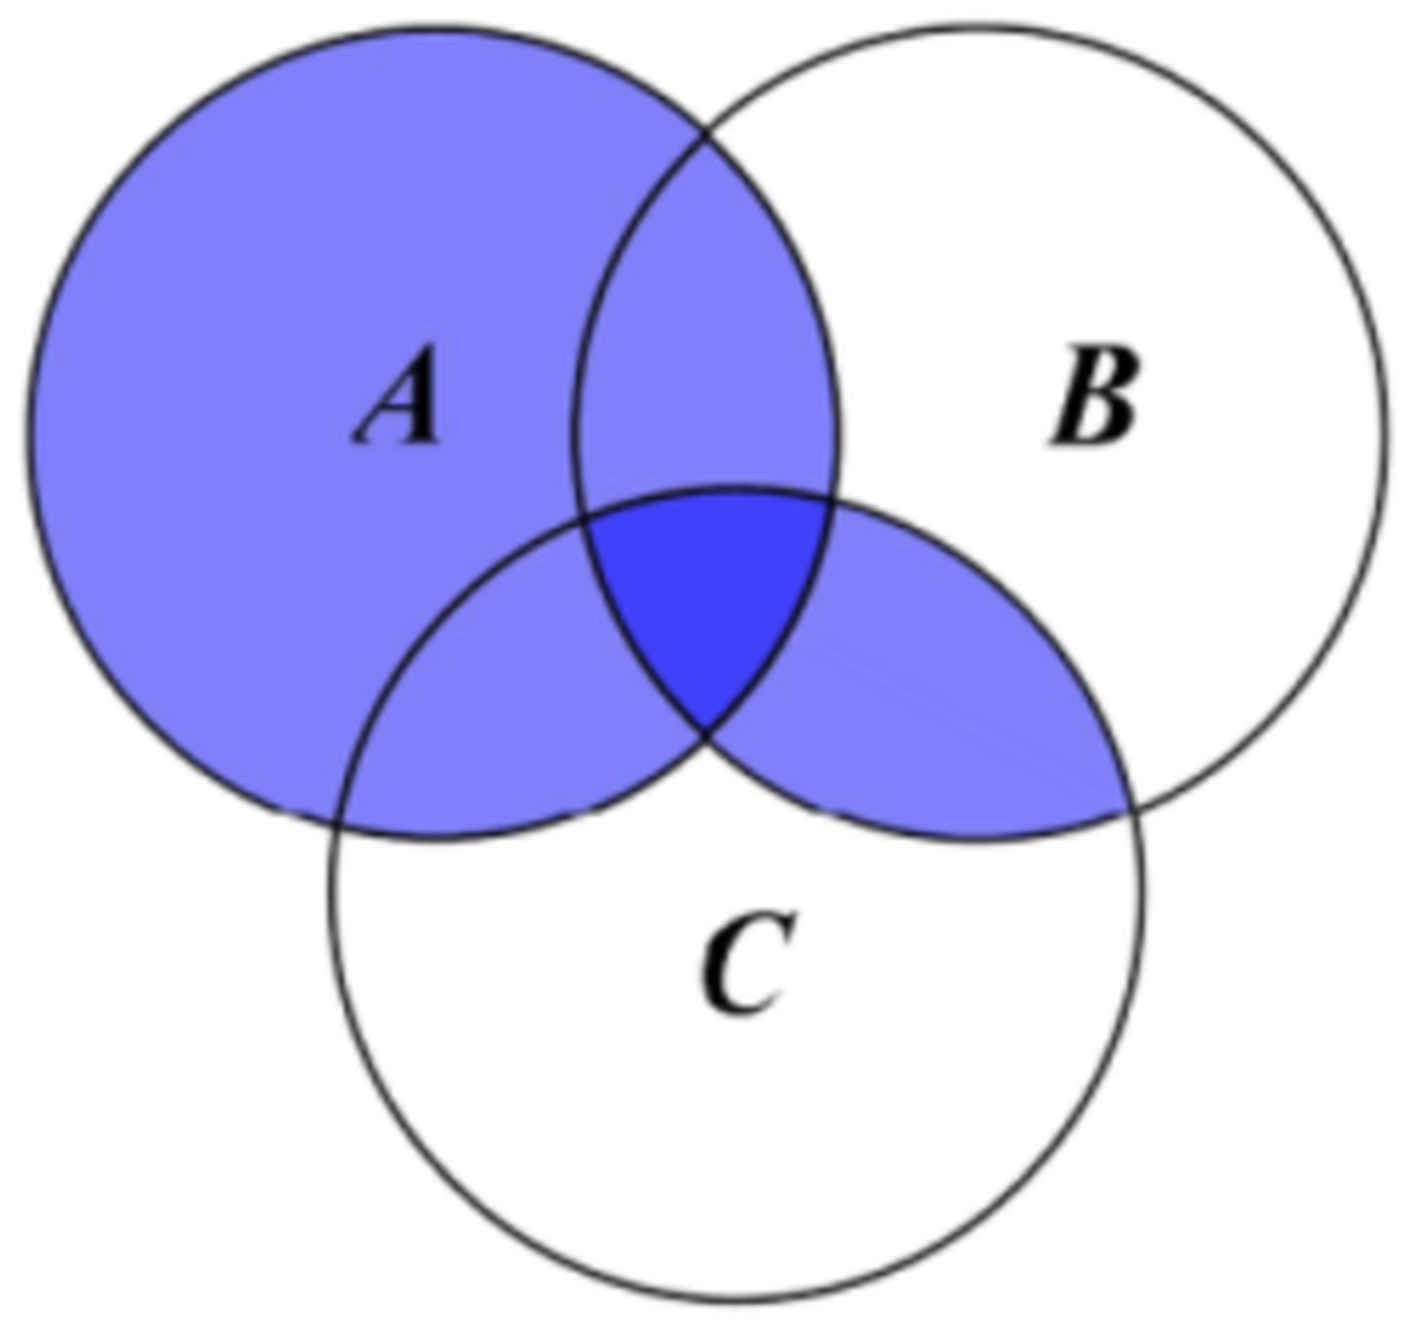
\includegraphics[width=0.30\textwidth]{figures/venn_A_union_BC.png}
\end{center}

\keepwithprev
A. $(A\cup C)\cap(B\cup C)$\qquad\qquad B. $(A\cup B)\cap(A\cup C)$

C. $(A\cup B)\cap(B\cup C)$\qquad\qquad D. $(A\cup B)\cap C$

\ans{$B$}

\ifanswer
\solbegin
\step{图中阴影部分表示元素满足是 $A$ 中的元素，或者是 $B$ 与 $C$ 的公共元素，}
\step{故可以表示为 $A\cup(B\cap C)$，也可以表示为 $(A\cup B)\cap(A\cup C)$.
故选 $B$.}
\solend

\fi

\item 设集合 $M=\left\{x\mid m\leqslant x\leqslant m+\dfrac34\right\}$，
$N=\left\{x\mid n-\dfrac13\leqslant x\leqslant n\right\}$，且 $M$、$N$ 都是集合
$\{x\mid0\leqslant x\leqslant1\}$ 的子集，如果把 $b-a$ 叫做集合
$\{x\mid a\leqslant x\leqslant b\}$ 的“长度”，那么集合 $M\cap N$ 的“长度”的
最小值是\mbox{（\quad）}

\keepwithprev
A. $\dfrac23$\qquad B. $\dfrac1{12}$\qquad C. $\dfrac13$\qquad D. $\dfrac5{12}$

\ans{$B$}

\ifanswer
\solbegin
\step{$M$ 的长度为 $\dfrac34$，$N$ 的长度为 $\dfrac13$，}
\step{当集合 $M\cap N$ 的长度的最小值时，$M$ 与 $N$ 应分别在区间 $[0,1]$ 的左右两端，}
\step{故 $M\cap N$ 的长度的最小值是 $\dfrac34+\dfrac13-1=\dfrac1{12}$，故选 $B$.}
\solend

\fi

\item 定义集合运算 $A-B=\{x\mid x\in A\text{ 且 }x\notin B\}$ 称为集合 $A$ 与集合 $B$ 的
差集；定义集合运算 $A\Delta B=(A-B)\cup(B-A)$ 称为集合 $A$ 与集合 $B$ 的对称差，
有以下 $4$ 个等式：① $A\Delta B=B\Delta A$；② $(A\Delta B)\Delta C=A\Delta(B\Delta C)$；
③ $A\cap(B\Delta C)=(A\cap B)\Delta(A\cap C)$；
④ $A\cup(B\Delta C)=(A\cup B)\Delta(A\cup C)$，
则 $4$ 个等式中恒成立的是\mbox{（\quad）}

\keepwithprev
A. ①②\qquad B. ①②③\qquad C. ①②④\qquad D. ①②③④

\ans{$B$}

\ifanswer
\solbegin
\step{对于①，由 $B\Delta A=(B-A)\cup(A-B)=(A-B)\cup(B-A)=A\Delta B$，
所以①正确；}
\step{对于②，由 $A-B=\{x\mid x\in A\text{ 且 }x\notin B\}
=\{x\mid x\in A,x\notin(A\cap B)\}=A-(A\cap B)$，}
\step{同理可得 $B-A=B-(A\cap B)$，}
\step{则 $A\Delta B=(A-B)\cup(B-A)=(A\cup B)-(A\cap B)$，}
\step{所以 $(A\Delta B)\Delta C=(A\Delta B)\cup C-(A\Delta B)\cap C$，}
\step{所以表示的集合为图（1）中阴影部分所表示的集合，如图所示，}
\step{同理 $A\Delta(B\Delta C)=A\cup(B\Delta C)-A\cap(B\Delta C)$，
也表示图（1）中阴影部分所表示的集合，}
\step{所以 $(A\Delta B)\Delta C=A\Delta(B\Delta C)$，所以②正确；}

\begin{center}
% 图取原卷截图、4× LANCZOS 放大（原卷印在下一页顶部，共三幅三圆韦恩图：
% 图（1）一幅、图（2）左右两幅，图（2）两幅下方各有一行式子标注）。
% 图只在【解析】里出现，故放进 \ifanswer 块，试卷版不排。
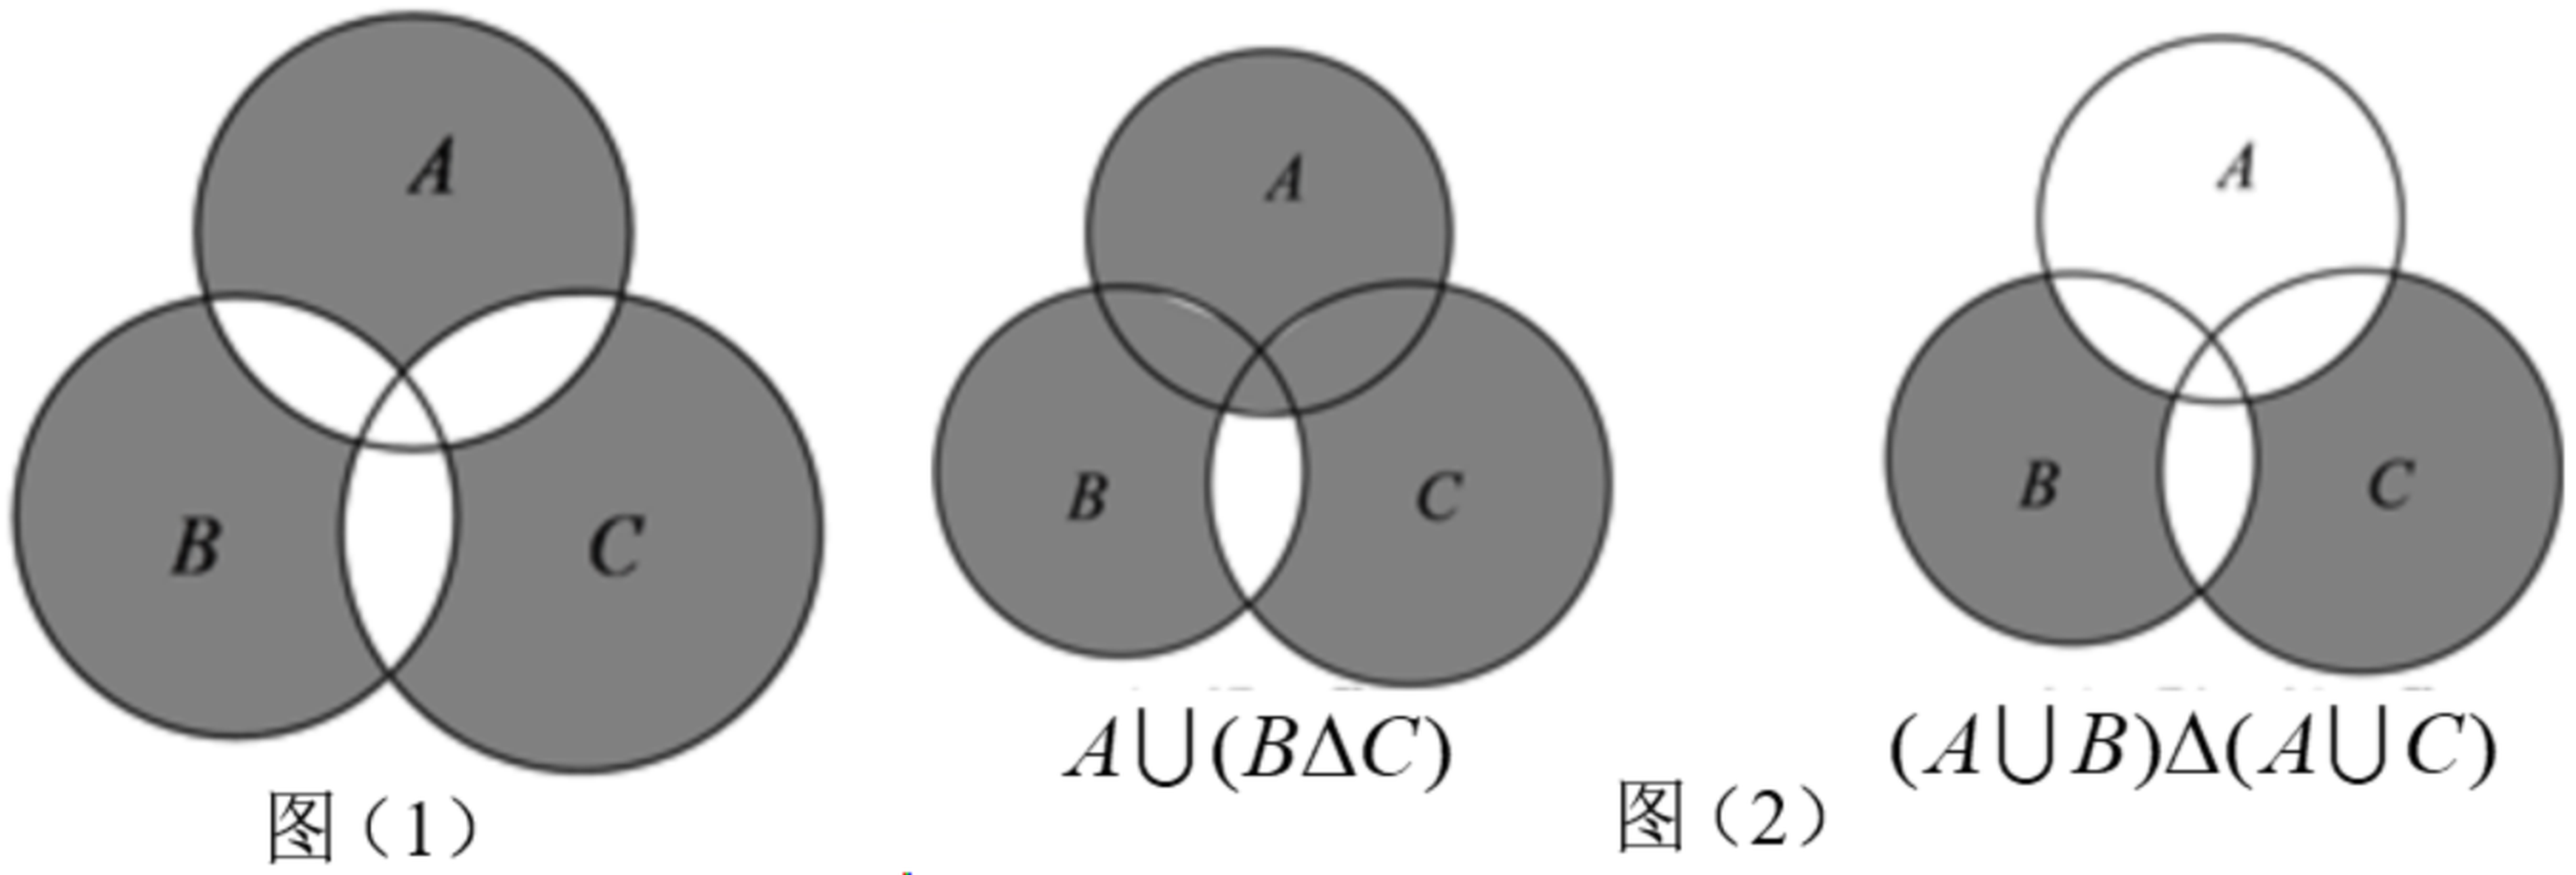
\includegraphics[width=0.86\textwidth]{figures/venn_symdiff3.png}
\end{center}

\step{对于③，由 $A\cap(B\Delta C)=A\cap(B\cup C-B\cap C)
=A\cap(B\cup C)-A\cap(B\cap C)$}
\step{$=(A\cap B)\cup(A\cap C)-(A\cap B)\cap(A\cap C)=(A\cap B)\Delta(A\cap C)$，
所以③正确；}
\step{对于④，如图（2）所示，$A\cup(B\Delta C)\neq(A\cup B)\Delta(A\cup C)$，
所以④错误.}
\step{故选 $B$.}
\solend

\fi

\end{enumerate}

\bigsec{三、解答题}

\begin{enumerate}
\setcounter{enumi}{16}

\item 已知集合 $M=\{x\mid a-1\leqslant x\leqslant2a+3\}$，$P=\{x\mid-2<x\leqslant4\}$，
全集 $U=\R$.

\begin{enumerate}[label=(\arabic*)]
\item 当 $a=2$ 时，求 $M\cap P$；
\item 若 $x\in P$ 是 $x\in M$ 的必要不充分条件，求实数 $a$ 的取值范围.
\end{enumerate}

\ifanswer
\solbegin
\stepm{(1)}{当 $a=2$ 时，集合 $M=\{x\mid1\leqslant x\leqslant7\}$，}
\step{所以 $M\cap P=\{x\mid1\leqslant x\leqslant4\}$；}
\stepm{(2)}{因为 $x\in P$ 是 $x\in M$ 的必要不充分条件，所以 $M\subset P$，}
\step{当 $M=\varnothing$ 时，$a-1>2a+3$，解得 $a<-4$，}
\step{当 $M\neq\varnothing$ 时，则
$\begin{cases}a-1\leqslant2a+3\\ a-1>-2\\ 2a+3\leqslant4\end{cases}$，
解得 $-1<a\leqslant\dfrac12$，}
\step{综上所述，实数 $a$ 的取值范围为
$(-\infty,-4)\cup\left(-1,\dfrac12\right]$.}
\solend

\fi

\ansspace[6]

\item 一辆汽车在某段路程中的行驶速度与时间的关系如图：

\begin{center}
% 图取原卷截图、4× LANCZOS 放大（速度—时间图：纵轴 $v/(\mathrm{km/h})$、
% 横轴 $t(\mathrm{h})$，$t\in[0,1]$、$[1,2]$、$[2,3]$ 三段矩形条高 50、80、90）。
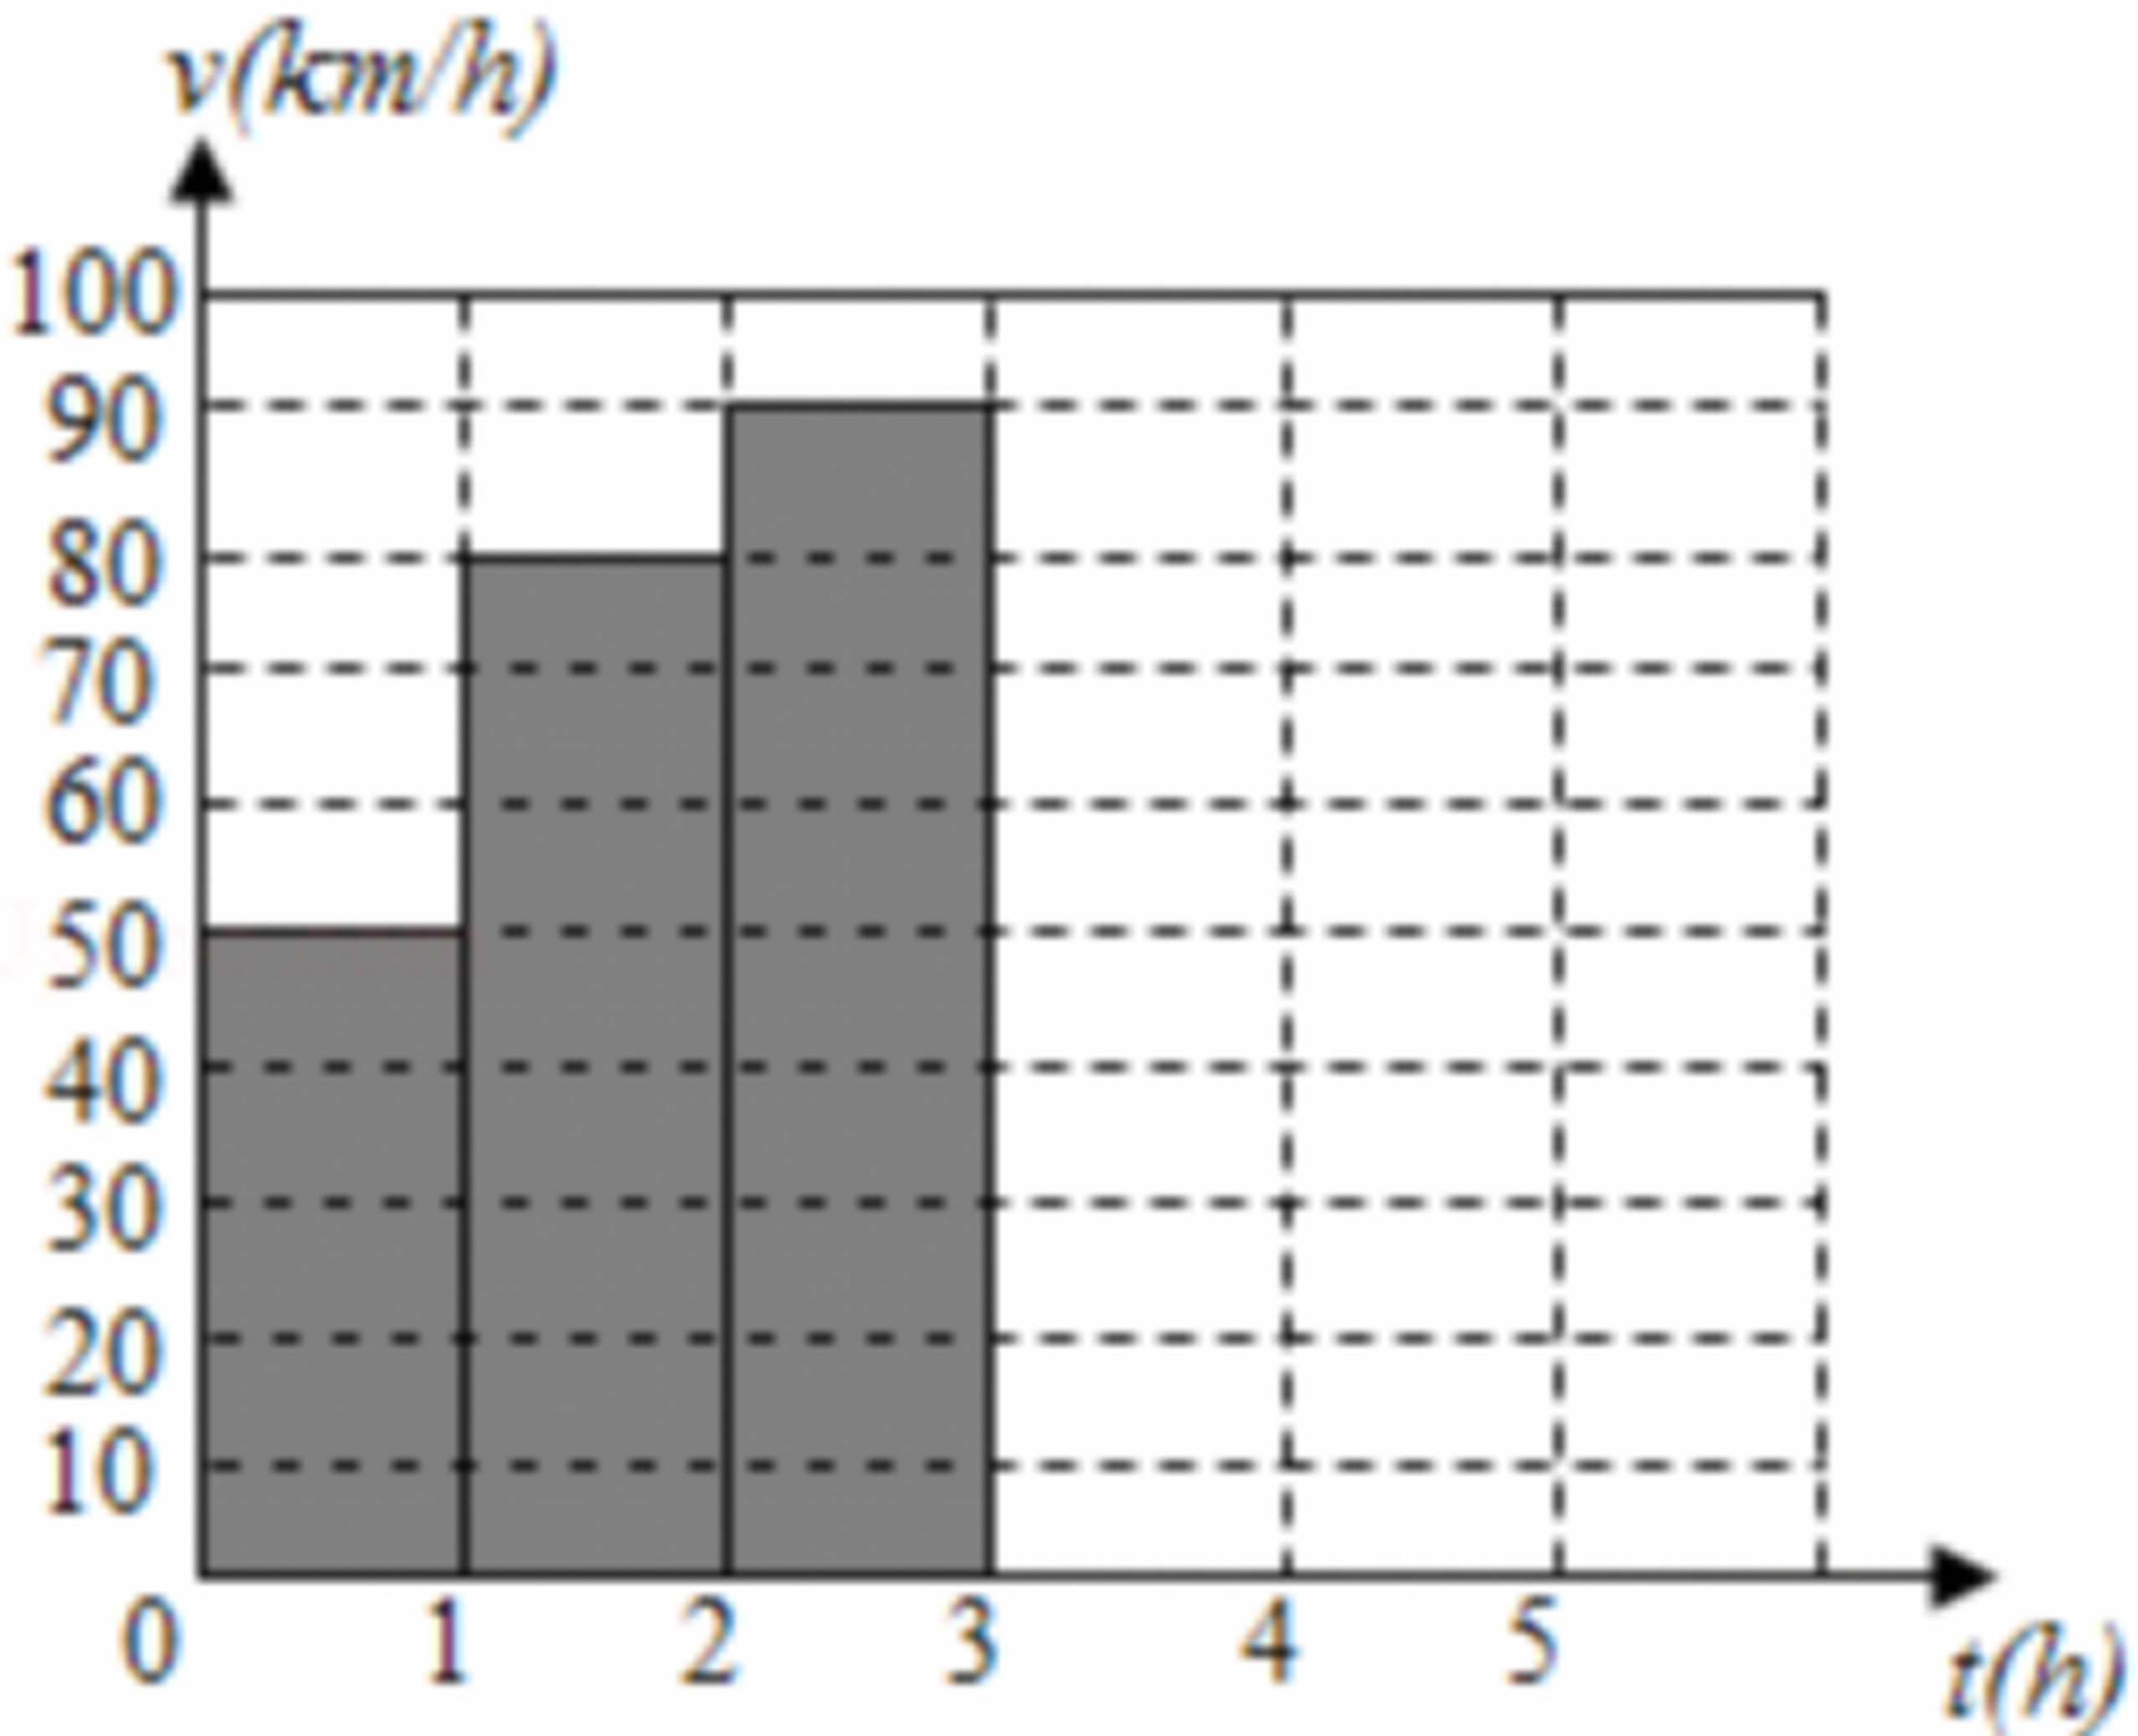
\includegraphics[width=0.52\textwidth]{figures/speed_time_bars.png}
\end{center}

\begin{enumerate}[label=(\arabic*)]
\item 求图中阴影部分的面积，并说明所求面积的实际意义；
\item 假设这辆汽车的里程表在汽车行驶这段路程前的读数为 $2004\,\mathrm{km}$，
试将汽车行驶这段路程时汽车里程表读数 $S$ 表示为时间 $t$ 的函数，
并求出当汽车里程表读数为 $2094\,\mathrm{km}$ 时，汽车行驶了多少时间？
\end{enumerate}

\ifanswer
\solbegin
\stepm{(1)}{由一辆汽车在某段路程中的行驶速度与时间的关系图，}
\step{得阴影部分的面积为 $50\times1+80\times1+90\times1=220$，}
\step{阴影部分的面积表示汽车在 $3$ 小时内行驶的路程为 $220\,\mathrm{km}$.}
\stepm{(2)}{$S=\begin{cases}
50t+2004,&0\leqslant t<1\\
80(t-1)+2054,&1\leqslant t<2\\
90(t-2)+2134,&2\leqslant t\leqslant3
\end{cases}$}
\step{令 $80(t-1)+2054=2094$，解得 $t=1.5$，所以汽车行驶 $1.5$ 小时.}
\solend

\fi

\ansspace[6]

\item 已知集合 $A=\{x\mid x<-2\text{ 或 }x\geqslant3\}$，$U=\R$.

\begin{enumerate}[label=(\arabic*)]
\item 求 $\overline{A}$；
\item 若 $B=\{x\mid mx-1>0\}$，当 $B\sub A$ 时，求实数 $m$ 的取值范围；
\item 若 $B=\{x\mid2m-6\leqslant x\leqslant m+4\}$，当 $B\cap\overline{A}=\varnothing$ 时，
求实数 $m$ 的取值范围.
\end{enumerate}

\ifanswer
\solbegin
\stepm{(1)}{因为集合 $A=\{x\mid x<-2\text{ 或 }x\geqslant3\}$，$U=\R$，
所以 $\overline{A}=\{x\mid-2\leqslant x<3\}$；}
\stepm{(2)}{当 $m=0$ 时，$B=\varnothing$，符合题意，}
\step{当 $m>0$ 时，$B=\left\{x\mid x>\dfrac1m\right\}$，则 $\dfrac1m\geqslant3$，
解得 $0<m\leqslant\dfrac13$，}
\step{当 $m<0$ 时，$B=\left\{x\mid x<\dfrac1m\right\}$，则 $\dfrac1m\leqslant-2$，
解得 $-\dfrac12\leqslant m<0$，}
\step{综上所述，实数 $m$ 的取值范围 $\left[-\dfrac12,\dfrac13\right]$；}
\stepm{(3)}{由题意得 $B=\{x\mid2m-6\leqslant x\leqslant m+4\}$，
$\overline{A}=\{x\mid-2\leqslant x<3\}$，且 $B\cap\overline{A}=\varnothing$，}
\step{当 $B=\varnothing$ 时，$2m-6>m+4$，解得 $m>10$，}
\step{当 $B\neq\varnothing$ 时，则 $\begin{cases}2m-6\leqslant m+4\\ m+4<-2\end{cases}$
或 $\begin{cases}2m-6\leqslant m+4\\ 2m-6\geqslant3\end{cases}$，}
\step{解得 $m<-6$ 或 $\dfrac92\leqslant m\leqslant10$，}
\step{综上所述，实数 $m$ 的取值范围为
$(-\infty,-6)\cup\left[\dfrac92,+\infty\right)$.}
\solend

\fi

\ansspace[8]

\item 在等腰梯形 $ABCD$ 中，$AB=DC=5$，$AD=4$，$BC=10$. 点 $E$ 在下底边 $BC$ 上.
点 $F$ 在腰 $AB$ 上.

\begin{center}
% 图取原卷截图、4× LANCZOS 放大（等腰梯形 $ABCD$ 与线段 $FE$，无辅助线）。
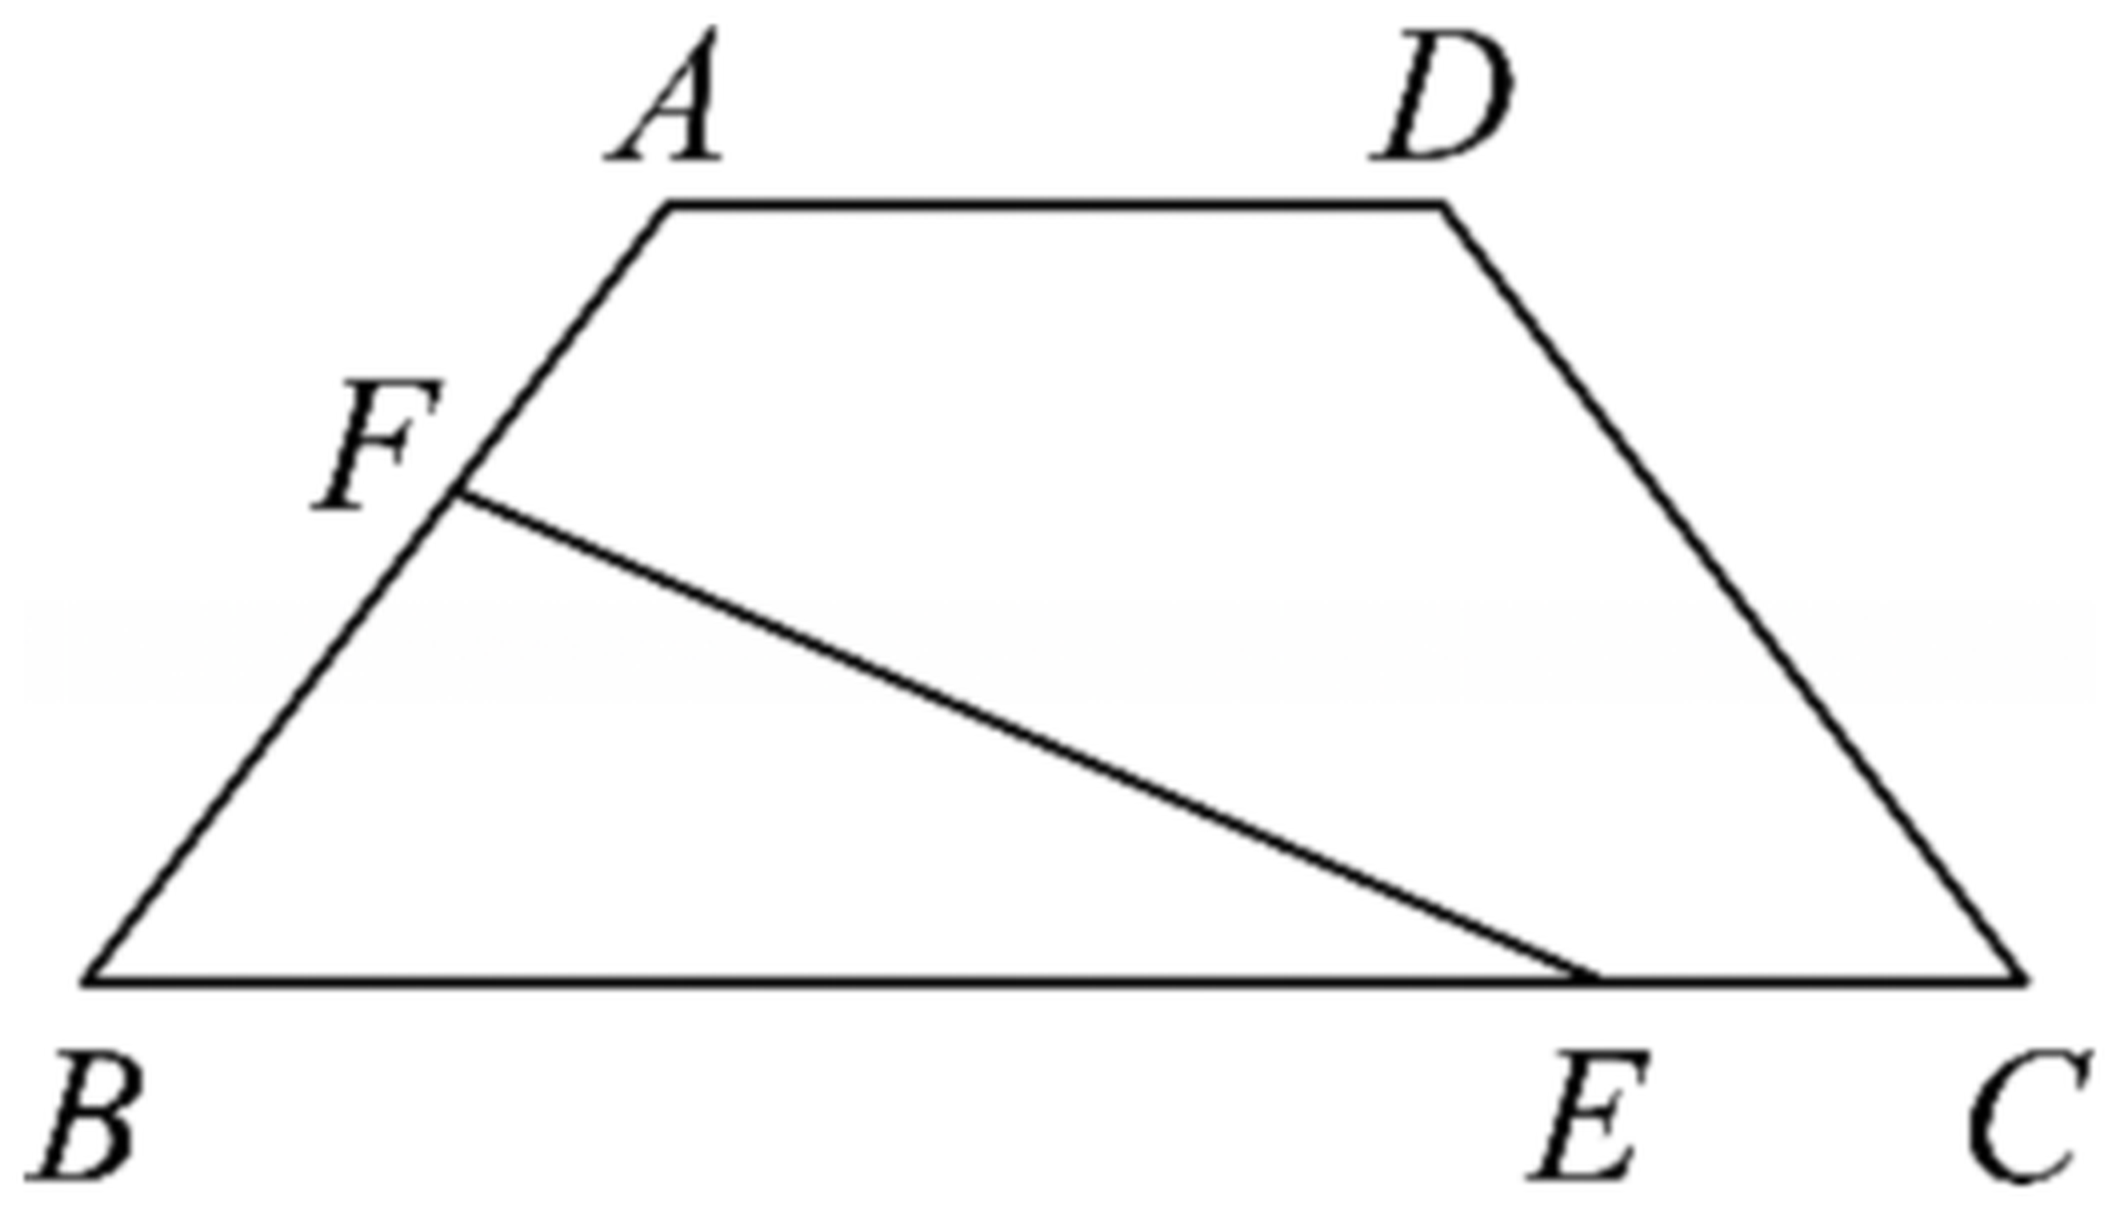
\includegraphics[width=0.46\textwidth]{figures/trapezoid_EF.png}
\end{center}

\begin{enumerate}[label=(\arabic*)]
\item 若 $EF$ 平分等腰梯形 $ABCD$ 的周长，设 $BE$ 长为 $x$，试用含 $x$ 的代数式表示
$\triangle BEF$ 的面积；
\item 是否存在线段 $EF$ 将等腰梯形 $ABCD$ 的周长和面积同时平分？若存在，求出此时 $BE$
的长；若不存在，请说明理由；
\item 是否存在线段 $EF$ 将等腰梯形 $ABCD$ 的周长和面积同时分成 $1:2$ 的两部分？
若存在，求此时 $BE$ 的长；若不存在，请说明理由.
\end{enumerate}

\ifanswer
\solbegin
\stepm{(1)}{过 $A$ 作 $AK\perp BC$ 交 $BC$ 于点 $K$，过 $F$ 作 $FG\perp BC$ 交 $BC$ 于点
$G$，}

\begin{center}
% 图取原卷截图、4× LANCZOS 放大（同梯形，多出虚线 $FG\perp BC$ 与 $AK\perp BC$
% 及两处直角符号；图只在【解析】里出现，故放进 \ifanswer 块）。
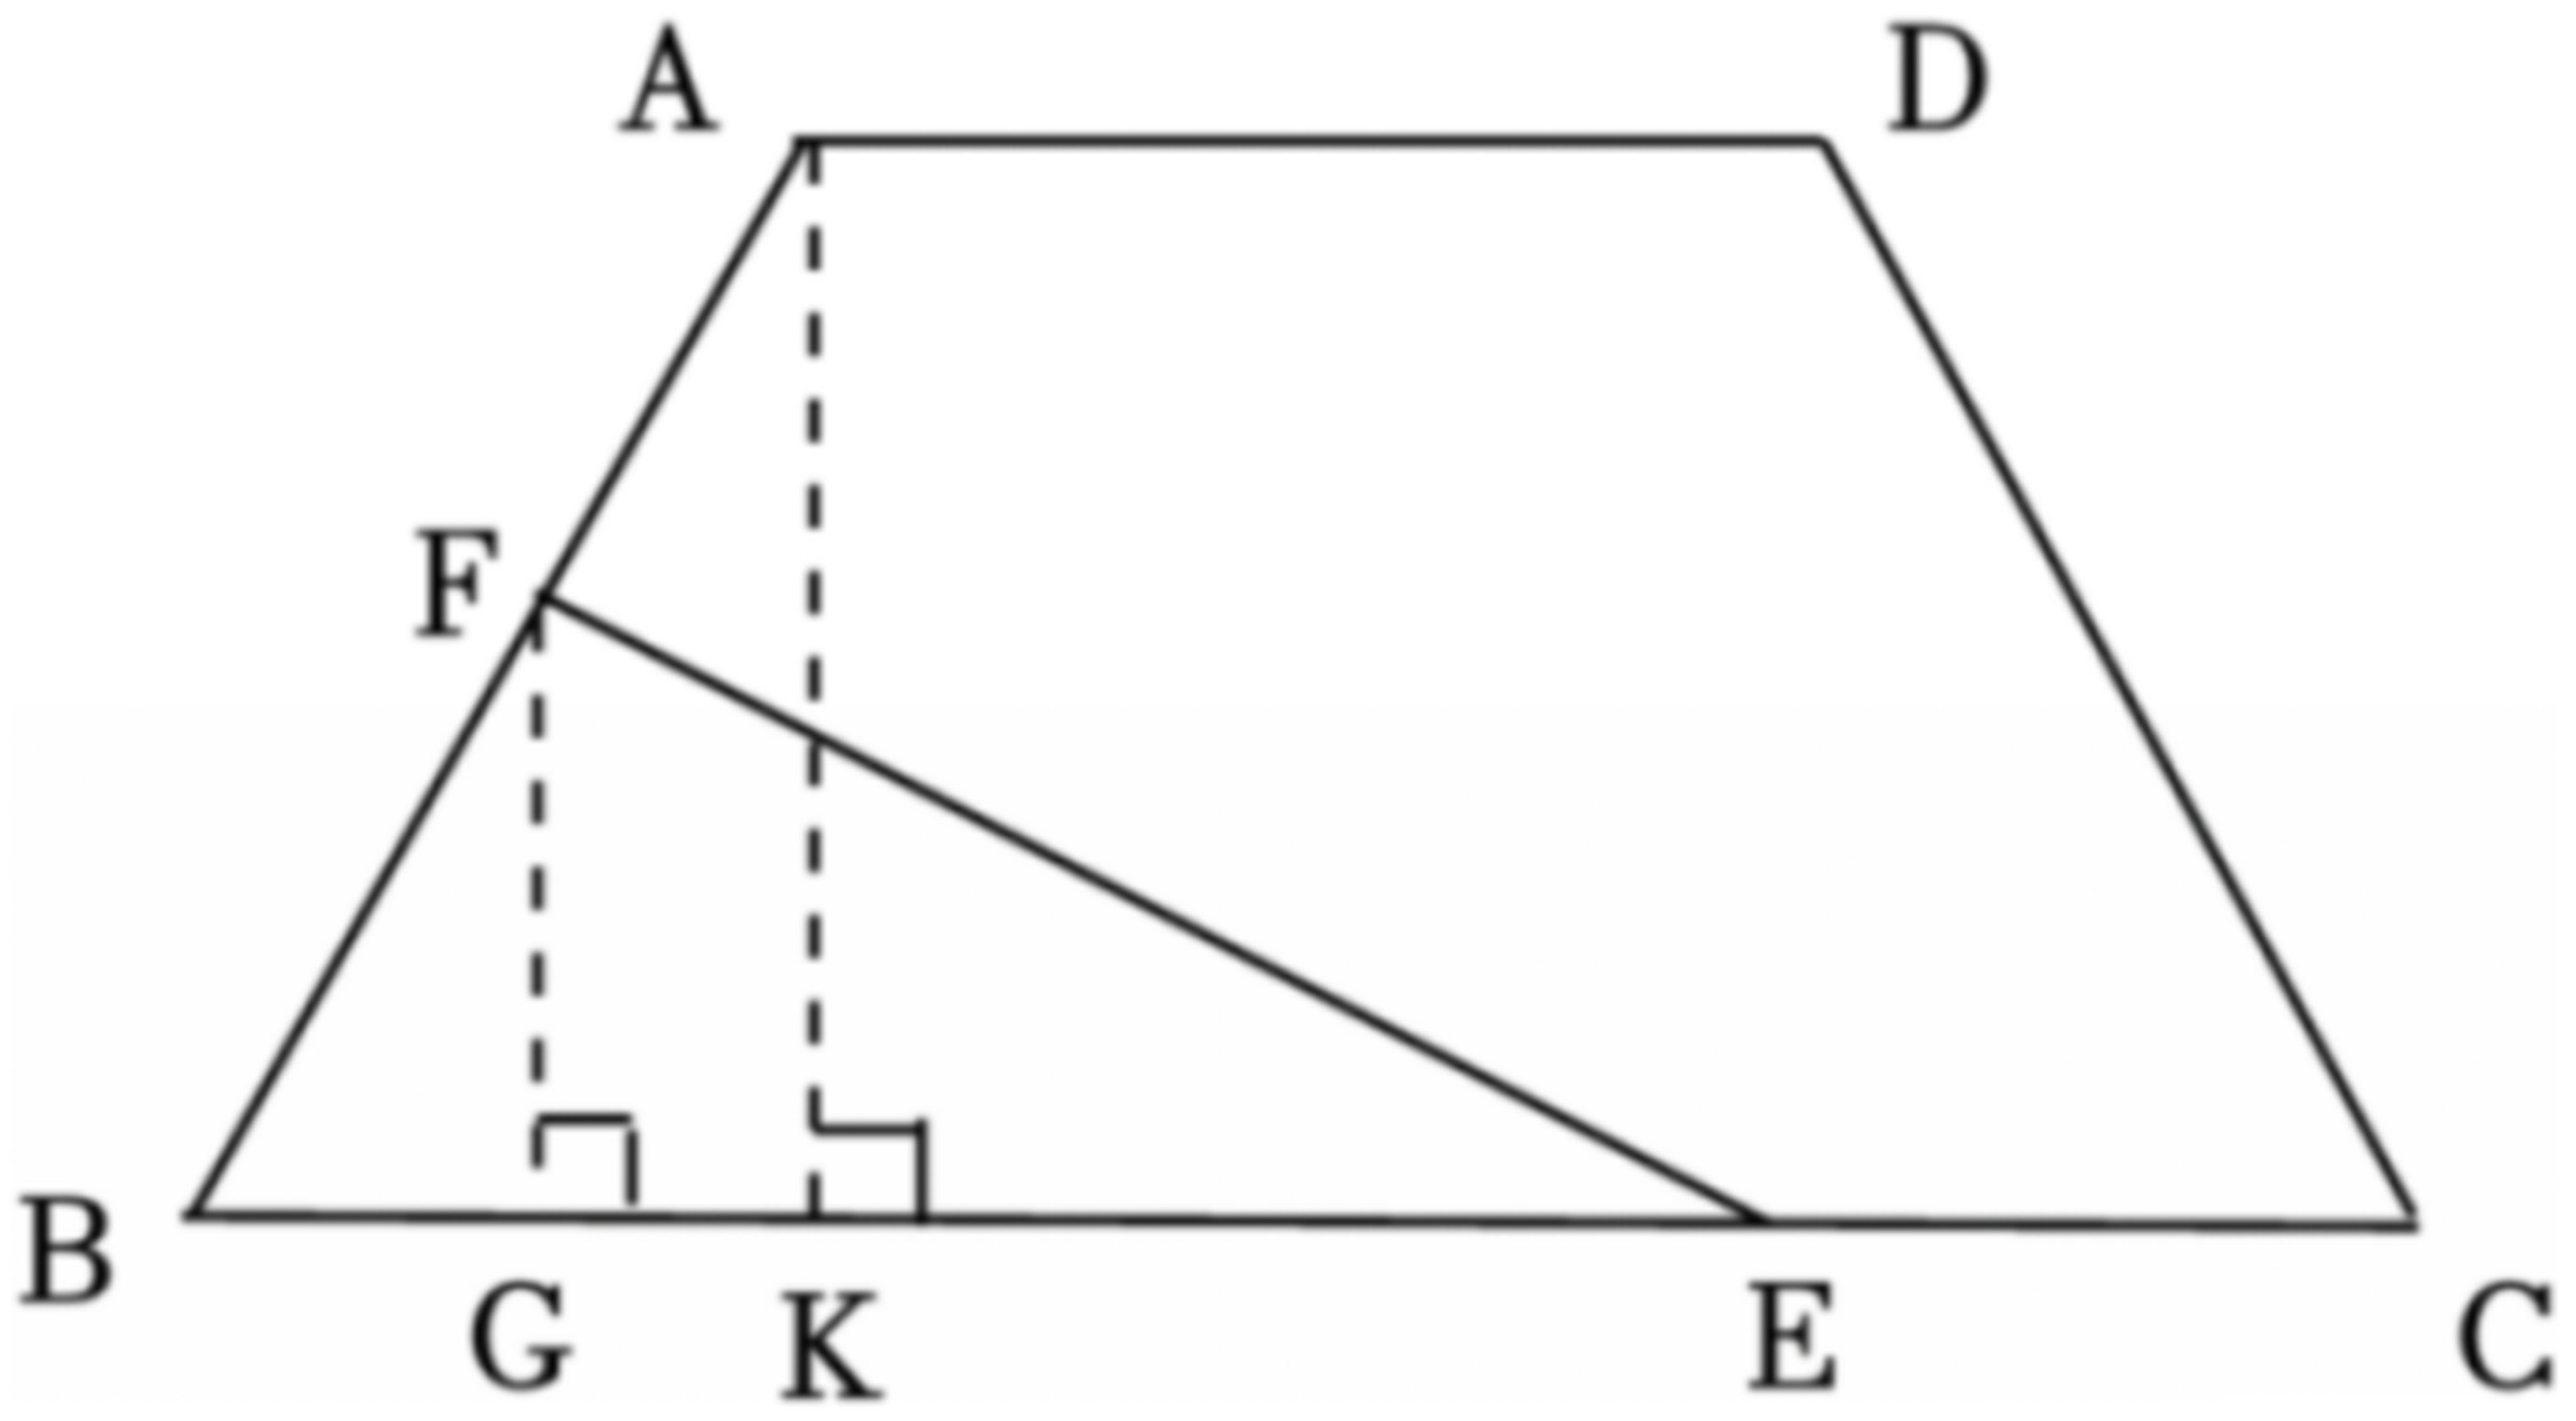
\includegraphics[width=0.62\textwidth]{figures/trapezoid_EF_aux.png}
\end{center}

\step{所以 $BK=\dfrac12\times(BC-AD)=\dfrac12\times(10-4)=3$，}
\step{$AK=\sqrt{AB^2-BK^2}=\sqrt{5^2-3^2}=4$，}
\step{由题意得，梯形 $ABCD$ 周长为 $24$，高为 $4$，面积为 $28$，}
\step{因为 $EF$ 平分等腰梯形 $ABCD$ 的周长，设 $BE$ 长为 $x$，则 $BF=12-x$，}
\step{由 $\begin{cases}0\leqslant12-x\leqslant5\\ 0\leqslant x\leqslant10\end{cases}$，
解得 $7\leqslant x\leqslant10$，}
\step{由题意得 $\triangle BFG\backsim\triangle BAK$，所以 $\dfrac{FG}{AK}=\dfrac{BF}{BA}$，
即 $\dfrac{FG}4=\dfrac{12-x}5$，}
\step{解得 $FG=\dfrac45(12-x)$，}
\step{所以 $S_{\triangle BEF}=\dfrac12BE\cdot FG
=-\dfrac25x^2+\dfrac{24}5x$（$7\leqslant x\leqslant10$）；}
\stepm{(2)}{存在，由 (1) 得 $-\dfrac25x^2+\dfrac{24}5x=\dfrac{28}2$，$x\in[7,10]$，}
\step{即 $x^2-12x+35=0$，解得 $x=7$ 或 $x=5$（舍去），}
\step{所以存在线段 $EF$ 将等腰梯形 $ABCD$ 的周长和面积同时平分，此时 $BE=7$；}
\stepm{(3)}{不存在，}
\step{情况一：$\triangle BEF$ 的面积$:$多边形 $AFECD$ 的面积 $=1:2$，
$(BE+BF):(AF+AD+DC+CE)=1:2$，}
\step{梯形周长的 $\dfrac13$ 是 $\dfrac{24}3=8$，面积的 $\dfrac13$ 是 $\dfrac{28}3$，}
\step{又因为 $BE=x$，所以 $BF=8-x$，}
\step{又因为 $\dfrac{FG}{AK}=\dfrac{BF}{BA}$，即 $\dfrac{FG}4=\dfrac{8-x}5$，
所以 $FG=\dfrac{32-4x}5$，}
\step{所以 $S_{\triangle BEF}=\dfrac12BE\times FG=-\dfrac25x^2+\dfrac{16}5x$，
所以 $\dfrac{28}3=-\dfrac25x^2+\dfrac{16}5x$，}
\step{整理得 $-3x^2+24x-70=0$，此时 $\Delta<0$，无解，故不存在；}
\step{情况二：$\triangle BEF$ 的面积$:$多边形 $AFECD$ 的面积 $=2:1$，
$(BE+BF):(AF+AD+DC+CE)=2:1$，}
\step{梯形周长的 $\dfrac13$ 为 $\dfrac{24}3=8$，面积的 $\dfrac13$ 为 $\dfrac{28}3$，
又 $BE=x$，所以 $BF=16-x$，}
\step{又 $\dfrac{FG}{AK}=\dfrac{BF}{BA}$，即 $\dfrac{FG}4=\dfrac{16-x}5$，
所以 $FG=\dfrac{64-4x}5$，}
\step{所以 $S_{\triangle BEF}=\dfrac12BE\times FG=-\dfrac25x^2+\dfrac{32}5x$，}
\step{所以 $\dfrac{28}3\times2=-\dfrac25x^2+\dfrac{32}5x$，
整理得 $-3x^2+48x-140=0$，}
\step{解得 $x=\dfrac{48+\sqrt{624}}6>10$，$x=\dfrac{48-\sqrt{624}}6<7$，
不符合题意，舍去，故不存在；}
\step{综上所述，不存在线段 $EF$ 将等腰梯形 $ABCD$ 的周长和面积同时分成 $1:2$ 的两部分.}
\solend

\fi

\ansspace[8]

\item 对集合 $\{1,2,\cdots,n\}$ 及其每一个非空子集 $A$，定义一个唯一确定的“交替和”
如下：将 $A$ 中的元素按照递减的次序排列，然后将第一个元素交替地减或加后继的元素所得的
结果，例如，子集 $\{1,2,4,6,9\}$ 的“交替和”是 $9-6+4-2+1=6$，子集 $\{5,6\}$ 的
“交替和”是 $6-5=1$，子集 $\{2\}$ 的交替和是 $2$；定义一个唯一确定的“交替积”如下：
将 $A$ 中的元素按照递减的次序排列，然后将第一个元素交替地除以或乘以后继的数所得的结果，
例如，集合 $\{1,2,4,6,9\}$ 的“交替积”是 $9\div6\times4\div2\times1=3$，
$\{5,6\}$ 的“交替积”是 $6\div5=1.2$，$\{2\}$ 的“交替积”是 $2$.

\begin{enumerate}[label=(\arabic*)]
\item 对于 $\{1,2,3,4,5,6,7,8,9\}$，求其所有子集的“交替和”的总和；
\item 对于 $\{1,2,\cdots,n\}$，求其所有子集的“交替和”的总和；
\item 对于 $\left\{n\mid\dfrac{495}{n+2}\in\N,n\in\Z\right\}$ 求其所有子集的
“交替积”的总和.
\end{enumerate}

\ifanswer
\solbegin
\stepm{(1)}{集合 $\{1,2,3,4,5,6,7,8,9\}$ 的子集中，除去 $\{9\}$ 外还有 $2^9-2$ 个
非空子集，}
\step{把这 $2^9-2$ 个非空子集两两组合后分别计算每一组中“交替和”之和，}
\step{组合原则是设 $A_i=\{9,a_1,a_2,\cdots\}$，$A_i^1=\{a_1,a_2,\cdots\}$，}
\step{集合 $A_i^1$ 的元素为集合 $A_i$ 中去掉 $9$ 的所有元素，把 $A_i$ 和 $A_i^1$
结合为一组，}
\step{显然，每组的“交替和”的和为 $9$，共有 $\dfrac{2^9-2}2$ 组，}
\step{所以，所有“交替和”之和应该为 $\dfrac{9(2^9-2)}2+9=2304$；}
\stepm{(2)}{集合 $\{1,2,\cdots,n\}$ 的子集中，除去 $\{n\}$ 外还有 $2^n-2$ 个非空子集，}
\step{把这 $2^n-2$ 个非空子集两两组合后分别计算每一组中“交替和”之和，}
\step{组合原则是设 $A_i=\{n,a_1,a_2,\cdots\}$，$A_i^1=\{a_1,a_2,\cdots\}$，}
\step{集合 $A_i^1$ 的元素为集合 $A_i$ 中去掉 $n$ 的所有元素，把 $A_i$ 和 $A_i^1$
结合为一组，}
\step{显然，每组的“交替和”的和为 $n$，共有 $\dfrac{2^n-2}2$ 组，}
% 注：下一行分子原卷印作花括号（其余同类处皆用圆括号），照抄未改，见文件头“原卷存疑”③。
\step{所以，所有“交替和”之和应该为 $\dfrac{n\{2^n-2\}}2+n=n\cdot2^{n-1}$；}
\stepm{(3)}{集合 $\left\{n\mid\dfrac{495}{n+2}\in\N,n\in\Z\right\}
=\{493,163,97,53,43,31,13,9,7,3,1,-1\}$，}
\step{其中除去 $\{-1\}$ 外还有 $2^{12}-2$ 个非空子集，}
% 注：下一行原卷把“把这”重复印了一次（“把这把这”），照抄未改，见文件头“原卷存疑”②。
\step{把这把这 $2^{12}-2$ 个非空子集两两组合后分别计算每一组中“交替积”之和，}
\step{组合原则是设 $A_j=\{-1,a_1,a_2,\cdots\}$，$A_j^1=\{a_1,a_2,\cdots\}$，}
\step{集合 $A_j^1$ 的元素为集合 $A_j$ 中去掉 $-1$ 的所有元素，把 $A_j$ 和 $A_j^1$
结合为一组，}
\step{显然，每组的“交替积”的和为 $0$，共有 $\dfrac{2^{12}-2}2$ 组，}
\step{所以，所有“交替积”之和应该为 $\dfrac{2^{12}-2}2\times0-1=-1$.}
\solend

\fi

\ansspace*[10]

\end{enumerate}

\end{document}
"
%
% 原始材料是微信公众号图文（公众号“魔都数学加油站”连载“27学年高一 30”，2026-09-23 发布，
% 原文标题“27学年高一30——2026-2027年上海市南洋模范中学高一上开学考”），
% 正文为 11 张 PNG 页。**同一篇里各页分辨率不一致**——第 2、3、9、10 页 4762×6735，
% 其余七页 2560×3620（已逐页打开确认，非下载缺档），取的是 mmbiz.qpic.cn/<hash>/0 的原图档。
% 原文本身就是一份**讲评版**：填空第 3—7 题下方印【答案】，第 8—12 题与其后各题印【解析】。
% 试题文字、答案与解析均照原卷录入，未改内容。卷面的粉色斜水印属水印，未录入。
%
% 卷首标题：原卷印作“2026-2027 年南洋模范中学高一上开学考”（公众号标题里的“上海市”
% 三字卷面标题行没有，本稿照卷面），年份区间按全稿惯例排 en dash，前缀照原卷保留“年”。
%
% 与原卷的排版差异（均已在 README“说明”中交代）：
%   ① 原文自**第 3 题**起（第 1、2 题未在该文中发布），故本稿题号亦自 3 起；
%   ② 原卷本就印有“一、填空题”“二、选择题”“三、解答题”三节标题，本稿照原卷分节，
%      只把标题改排成全稿统一的“大节标题”样式；
%   ③ 原卷填空第 3—7 题只印【答案】行、第 8 题起印【解析】（选择题答案写在解析末句
%      “故选 D／B”里），本稿统一改为试卷版隐去、答案版以 \ans{}／\ifanswer 块给出，
%      两版彻底分离；
%   ④ 子集符号原卷两种并用：第 7 题题干两处、第 19(2) 题作带下划线的 $\subseteq$，
%      第 17(2) 题解析作真包含的 $\subset$，本稿分别照录为 $\sub$ 与 $\subset$；
%   ⑤ 补集符号原卷一律作**上横线**（$\overline{A}$、$\overline{B}$），本稿照录；
%   ⑥ 原卷的实数集 R 一律作斜体（第 4 题、第 17 题与第 19 题题干的 $U=R$），
%      第 21(3) 题的自然数集与整数集作**粗体** $\mathbf{N}$、$\mathbf{Z}$，
%      本稿按全稿惯例统一写作 $\R$、$\N$、$\Z$；
%   ⑦ 原卷填空的横线约两个字宽，本稿按全稿惯例统一排 \blankline[4.4em]；
%   ⑧ 原卷未印副标题，本稿按全稿惯例补出副标题“集合与常用逻辑用语”——但本卷是开学考，
%      范围不止这一章：第 18 题是速度—时间图象题、第 20 题是等腰梯形的周长/面积平分问题，
%      副标题只标了主章节（见文末“高一30 专记”）；
%   ⑨ 第 13、14、18、20 题的图印在题干右侧、第 16 题的三幅图印在【解析】里的下一页顶部、
%      第 20 题【解析】另有一张带辅助线的图，本稿一律移至题干或解析之后；
%      图取原卷截图、4× LANCZOS 放大（见各 \includegraphics 前的注释）。
%
% 原卷存疑三处（均照抄原卷、未改，见源码中该处上方注释）：
%   ① 第 10 题【解析】验证“破晓集”时写的是 $\notin A$、$\in A$（如“$-2-2=-4\notin A$”），
%      但该处讨论的集合原题设里叫 $P$，同题②的“$x+y=2(k_1+k_2)\in A$”亦然——
%      本稿照抄未改（按文意应为 $P$）；
%   ② 第 21 题【解析】(3) 有“把这把这 $2^{12}-2$ 个非空子集”（“把这”重复印了一次）；
%   ③ 同题 (2) 的结论式分子原卷印作花括号 $\dfrac{n\{2^n-2\}}{2}$（其余同类处皆用圆括号）。

\documentclass[a4paper,11pt]{article}
\usepackage{common}

\begin{document}

\examtitlest[3]{2026--2027 年南洋模范中学高一上开学考}{集合与常用逻辑用语}

\bigsec{一、填空题}

\begin{enumerate}
\setcounter{enumi}{2}

\item 若集合 $A=\{x\mid x^2-2kx+7k=0\}$ 有且仅有三个真子集，则 $k$ 的取值范围是
\blankline[4.4em].

\ans{$(-\infty,0)\cup(7,+\infty)$}

\item “存在 $x\in\R$，使得 $x^2+2x+5=0$”的否定形式是 \blankline[4.4em].

\ans{对任何 $x\in\R$，都有 $x^2+2x+5\neq0$}

\item 下列命题中，$p$ 是 $q$ 的必要非充分条件的是 \blankline[4.4em].

① $p:x>2$ 且 $y>3$，$q:x+y>5$；

② $p$：四边形的四个角都相等，$q$：四边形是正方形.

\ans{②}

\item 若“条件 $\alpha:2\leqslant x\leqslant4$”是“条件 $\beta:3m-1\leqslant x\leqslant-m$”的
充分非必要条件，则 $m$ 的取值范围是 \blankline[4.4em].

\ans{$(-\infty,-4]$}

\item 满足 $\{1\}\sub M\sub\{1,2,4,5\}$ 的集合 $M$ 的个数为 \blankline[4.4em] 个.

\ans{$8$}

\item 已知集合 $A=\{1,2\}$，集合 $B=\{x\mid ax=6\}$，若 $A\cup B=A$，则 $a$ 的所有取值
构成的集合为 \blankline[4.4em].

\ifanswer
\solbegin
\step{因为 $A\cup B=A$，所以 $B\sub A$，}
\step{当 $a=0$ 时，$B=\varnothing$，满足 $B\sub A$；}
\step{当 $a\neq0$ 时，$B=\left\{\dfrac6a\right\}$，则 $\dfrac6a=1$ 或 $\dfrac6a=2$，
解得 $a=6$ 或 $a=3$，}
\step{综上所述，$a$ 的所有取值构成的集合为 $\{0,3,6\}$.}
\solend

\fi

\item 对于集合 $M$、$N$，定义 $M-N=\{x\mid x\in M\text{ 且 }x\notin N\}$，
$M\oplus N=(M-N)\cup(N-M)$，设 $A=\{y\mid y=|x|,x\in\R\}$，
$B=\{y\mid y=-(x-1)^2+2,x\in\R\}$，则 $A\oplus B=$ \blankline[4.4em].

\ifanswer
\solbegin
\step{由已知 $A=[0,+\infty)$，$B=(-\infty,2]$，}
\step{由于 $A-B=(2,+\infty)$，$B-A=(-\infty,0)$，}
\step{故 $A\oplus B=(A-B)\cup(B-A)=(-\infty,0)\cup(2,+\infty)$.}
\solend

\fi

\item 设 $P$ 为非空实数集满足：对任意给定的 $x$、$y\in P$（$x$、$y$ 可以相同），都有
$x+y\in P$，$x-y\in P$，$xy\in P$，则称 $P$ 为破晓集. 关于破晓集有下列结论：
①集合 $P=\{-2,-1,0,1,2\}$ 为破晓集；②集合 $P=\{x\mid x=2n,n\in\Z\}$ 为破晓集；
③若集合 $P_1$、$P_2$ 为破晓集，则 $P_1\cup P_2$ 为破晓集；④若集合 $P$ 为破晓集，
则一定有 $0\in P$；⑤若集合 $P_1$、$P_2$ 为破晓集，则 $P_1\cap P_2$ 为破晓集；
其中正确结论的序号是 \blankline[4.4em].

\ifanswer
\solbegin
% 注：以下几步原卷把该集合记作 $A$（题设里叫 $P$），照抄未改，见文件头“原卷存疑”①。
\step{对于①：$-2-2=-4\notin A$，故集合 $P=\{-2,-1,0,1,2\}$ 不为破晓集，故①错误；}
\step{②设 $x$、$y\in A$，则 $x=2k_1$，$y=2k_2$，且 $k_1$、$k_2\in\Z$，}
\step{故 $x+y=2(k_1+k_2)\in A$，$x-y=2(k_1-k_2)\in A$，$xy=4k_1k_2\in A$，}
\step{故集合 $P=\{x\mid x=2n,n\in\Z\}$ 为破晓集，故②正确；}
\step{③若集合 $P_1$、$P_2$ 为破晓集，设 $P_1=\{x\mid x=2k,k\in\Z\}$，
$P_2=\{x\mid x=3k,k\in\Z\}$，}
\step{但是 $P_1\cup P_2$ 不为破晓集，如 $x=2$，$y=3$ 时，$x+y=5$，
故 $5\notin(P_1\cup P_2)$，故③错误；}
\step{④若集合 $P$ 为破晓集，则取 $x=y$，$x-y=0\in A$，则一定有 $0\in P$，故④正确.}
\step{⑤正确；}
\step{故正确的是②④⑤.}
\solend

\fi

\item 已知集合 $M$ 的元素均为正整数，定义集合 $M$ 的“变项和”为：将 $M$ 中每个元素 $m$
都乘以 $(-1)^m$ 后再求和. 若集合 $A=\{n\mid1\leqslant n\leqslant10,n\in\N\}$，则集合 $A$
的所有非空子集的“变项和”的总和为 \blankline[4.4em].

\ifanswer
\solbegin
\step{$A$ 集合的所有非空子集中，每个元素出现的次数都是
$(2^{10}-1)-(2^9-1)=2^9$，}
\step{则集合 $A$ 的所有非空子集的“变项和”的总和为
$1\times(-1)^1\times2^9+2\times(-1)^2\times2^9+\cdots+10\times(-1)^{10}\times2^9$}
\step{$=(-1+2-3+4-\cdots-9+10)\times2^9=5\times2^9=2560$.}
\solend

\fi

\item 已知集合 $A=[t,t+1]\cup[t+4,t+9]$，$0\notin A$，存在正数 $\lambda$，使得对任意
$a\in A$，都有 $\dfrac\lambda a\in A$，则 $t$ 的值是 \blankline[4.4em].

\ifanswer
\solbegin
\step{当 $t>0$ 时，当 $a\in[t,t+1]$ 时，$\dfrac\lambda a\in[t+4,t+9]$，}
\step{当 $a\in[t+4,t+9]$ 时，$\dfrac\lambda a\in[t,t+1]$，}
\step{即当 $a=t$ 时，$\dfrac\lambda a\leqslant t+9$；当 $a=t+9$ 时，
$\dfrac\lambda a\geqslant t$，即 $\lambda=t(t+9)$；}
\step{当 $a=t+1$ 时，$\dfrac\lambda a\geqslant t+4$，当 $a=t+4$ 时，
$\dfrac\lambda a\leqslant t+1$，即 $\lambda=(t+1)(t+4)$，}
\step{所以 $t(t+9)=(t+1)(t+4)$，解得 $t=1$.}
\step{当 $t+1<0<t+4$ 时，当 $a\in[t,t+1]$ 时，$\dfrac\lambda a\in[t,t+1]$.}
\step{当 $a\in[t+4,t+9]$ 时，则 $\dfrac\lambda a\in[t+4,t+9]$，}
\step{即当 $a=t$ 时，$\dfrac\lambda a\leqslant t+1$，当 $a=t+1$ 时，
$\dfrac\lambda a\geqslant t$，即 $\lambda=t(t+1)$，}
\step{即当 $a=t+4$ 时，$\dfrac\lambda a\leqslant t+9$，当 $a=t+9$ 时，
$\dfrac\lambda a\geqslant t+4$，即 $\lambda=(t+4)(t+9)$，}
\step{所以 $t(t+1)=(t+4)(t+9)$，解得 $t=-3$.}
\step{当 $t+9<0$ 时，同理可得无解.}
\step{综上，$t$ 的值为 $1$ 或 $-3$.}
\solend

\fi

\end{enumerate}

\bigsec{二、选择题}

\begin{enumerate}
\setcounter{enumi}{12}

% 这道题是“题干 + 图 + 选项”约 6cm 的一整块，页末放不下就会被拆开（切页审计的 A 类），
% 故在题前先量一次页高：不够就把整道题干连图带选项一起挪到次页。
\needvspace{6.5cm}
\item 设 $U=\{1,2,3,4,5\}$，$A$、$B$ 都是 $U$ 的子集，且 $A\cap B=\{5\}$，
$\overline{A}\cap B=\{4\}$，$\overline{A}\cap\overline{B}=\{1,2\}$，
则以下四个判断中正确的是\mbox{（\quad）}

\begin{center}
% 图取原卷截图、4× LANCZOS 放大（原卷把图印在题干右侧，本稿移至此处，见文件头⑨）。
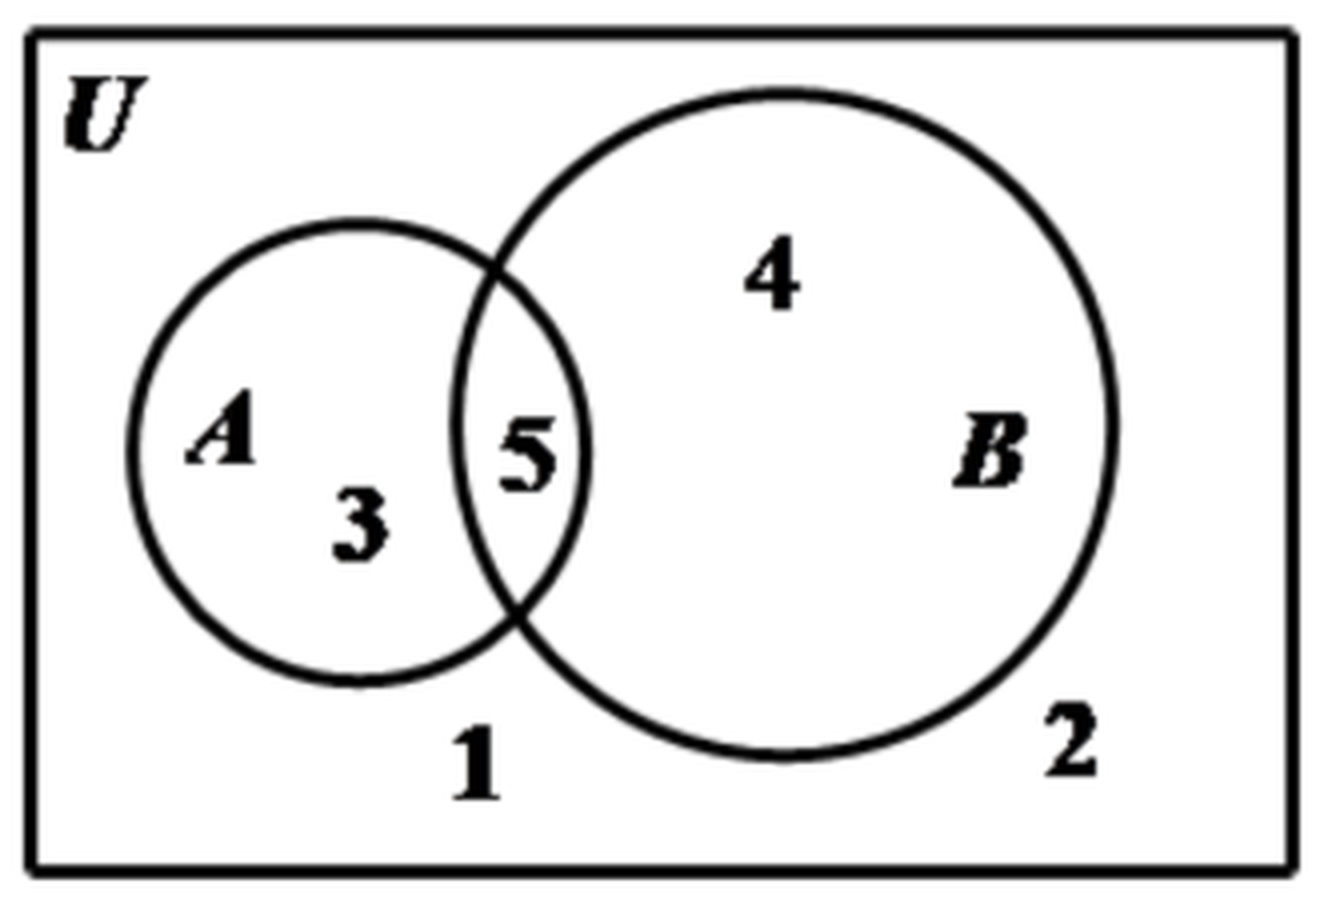
\includegraphics[width=0.28\textwidth]{figures/venn_U5_AB.png}
\end{center}

\keepwithprev
A. $3\notin A$ 且 $3\notin B$\qquad\qquad B. $3\in A$ 且 $3\in B$

C. $3\notin A$ 且 $3\in B$\qquad\qquad D. $3\in A$ 且 $3\notin B$

\ans{$D$}

\ifanswer
\solbegin
\step{画出韦恩图，得 $A=\{5,3\}$，$B=\{5,4\}$，}
\step{则 $3\in A$ 且 $3\notin B$. 故选 $D$.}
\solend

\fi

% 同第 13 题：整块（题干 + 图 + 选项）在答案版还要再挂【答案】【解析】，页末更易被拆开。
\needvspace{7.5cm}
\item 如图表示图形阴影部分的是\mbox{（\quad）}

\begin{center}
% 图取原卷截图、4× LANCZOS 放大（三圆 $A$、$B$、$C$，阴影为整个 $A$ 圆加 $B\cap C$）。
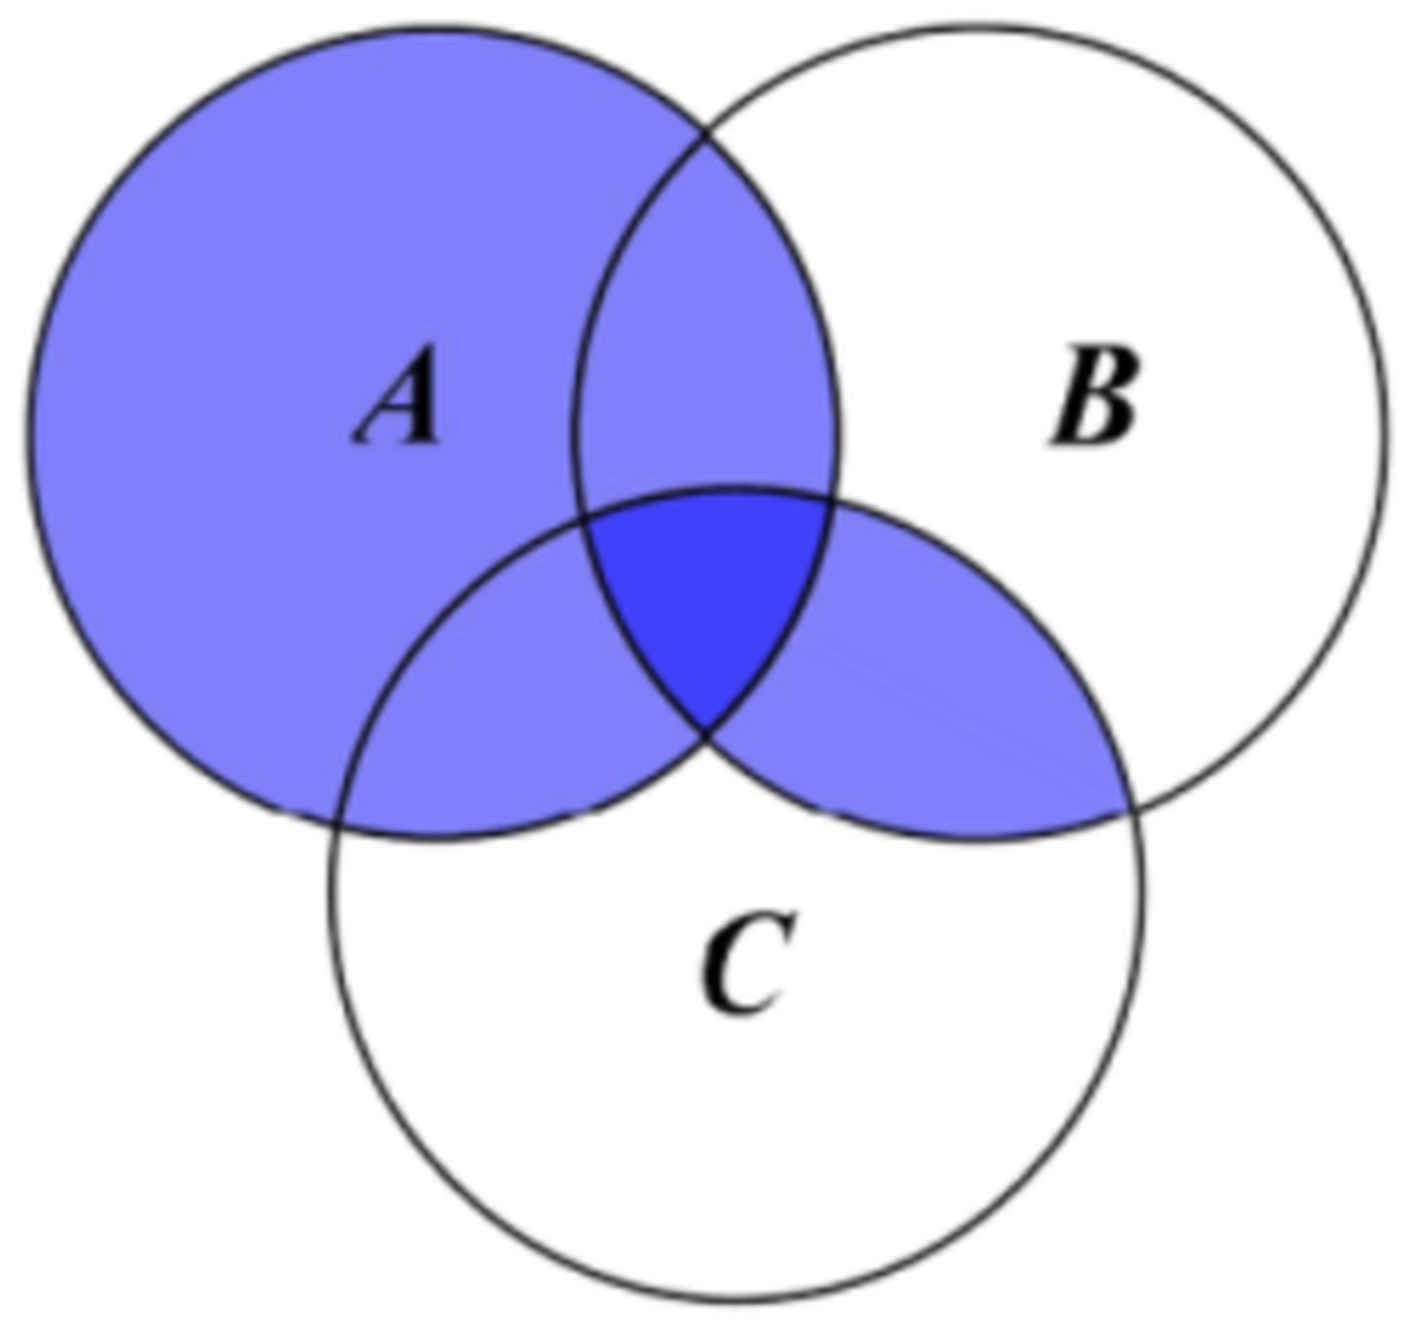
\includegraphics[width=0.30\textwidth]{figures/venn_A_union_BC.png}
\end{center}

\keepwithprev
A. $(A\cup C)\cap(B\cup C)$\qquad\qquad B. $(A\cup B)\cap(A\cup C)$

C. $(A\cup B)\cap(B\cup C)$\qquad\qquad D. $(A\cup B)\cap C$

\ans{$B$}

\ifanswer
\solbegin
\step{图中阴影部分表示元素满足是 $A$ 中的元素，或者是 $B$ 与 $C$ 的公共元素，}
\step{故可以表示为 $A\cup(B\cap C)$，也可以表示为 $(A\cup B)\cap(A\cup C)$.
故选 $B$.}
\solend

\fi

\item 设集合 $M=\left\{x\mid m\leqslant x\leqslant m+\dfrac34\right\}$，
$N=\left\{x\mid n-\dfrac13\leqslant x\leqslant n\right\}$，且 $M$、$N$ 都是集合
$\{x\mid0\leqslant x\leqslant1\}$ 的子集，如果把 $b-a$ 叫做集合
$\{x\mid a\leqslant x\leqslant b\}$ 的“长度”，那么集合 $M\cap N$ 的“长度”的
最小值是\mbox{（\quad）}

\keepwithprev
A. $\dfrac23$\qquad B. $\dfrac1{12}$\qquad C. $\dfrac13$\qquad D. $\dfrac5{12}$

\ans{$B$}

\ifanswer
\solbegin
\step{$M$ 的长度为 $\dfrac34$，$N$ 的长度为 $\dfrac13$，}
\step{当集合 $M\cap N$ 的长度的最小值时，$M$ 与 $N$ 应分别在区间 $[0,1]$ 的左右两端，}
\step{故 $M\cap N$ 的长度的最小值是 $\dfrac34+\dfrac13-1=\dfrac1{12}$，故选 $B$.}
\solend

\fi

\item 定义集合运算 $A-B=\{x\mid x\in A\text{ 且 }x\notin B\}$ 称为集合 $A$ 与集合 $B$ 的
差集；定义集合运算 $A\Delta B=(A-B)\cup(B-A)$ 称为集合 $A$ 与集合 $B$ 的对称差，
有以下 $4$ 个等式：① $A\Delta B=B\Delta A$；② $(A\Delta B)\Delta C=A\Delta(B\Delta C)$；
③ $A\cap(B\Delta C)=(A\cap B)\Delta(A\cap C)$；
④ $A\cup(B\Delta C)=(A\cup B)\Delta(A\cup C)$，
则 $4$ 个等式中恒成立的是\mbox{（\quad）}

\keepwithprev
A. ①②\qquad B. ①②③\qquad C. ①②④\qquad D. ①②③④

\ans{$B$}

\ifanswer
\solbegin
\step{对于①，由 $B\Delta A=(B-A)\cup(A-B)=(A-B)\cup(B-A)=A\Delta B$，
所以①正确；}
\step{对于②，由 $A-B=\{x\mid x\in A\text{ 且 }x\notin B\}
=\{x\mid x\in A,x\notin(A\cap B)\}=A-(A\cap B)$，}
\step{同理可得 $B-A=B-(A\cap B)$，}
\step{则 $A\Delta B=(A-B)\cup(B-A)=(A\cup B)-(A\cap B)$，}
\step{所以 $(A\Delta B)\Delta C=(A\Delta B)\cup C-(A\Delta B)\cap C$，}
\step{所以表示的集合为图（1）中阴影部分所表示的集合，如图所示，}
\step{同理 $A\Delta(B\Delta C)=A\cup(B\Delta C)-A\cap(B\Delta C)$，
也表示图（1）中阴影部分所表示的集合，}
\step{所以 $(A\Delta B)\Delta C=A\Delta(B\Delta C)$，所以②正确；}

\begin{center}
% 图取原卷截图、4× LANCZOS 放大（原卷印在下一页顶部，共三幅三圆韦恩图：
% 图（1）一幅、图（2）左右两幅，图（2）两幅下方各有一行式子标注）。
% 图只在【解析】里出现，故放进 \ifanswer 块，试卷版不排。
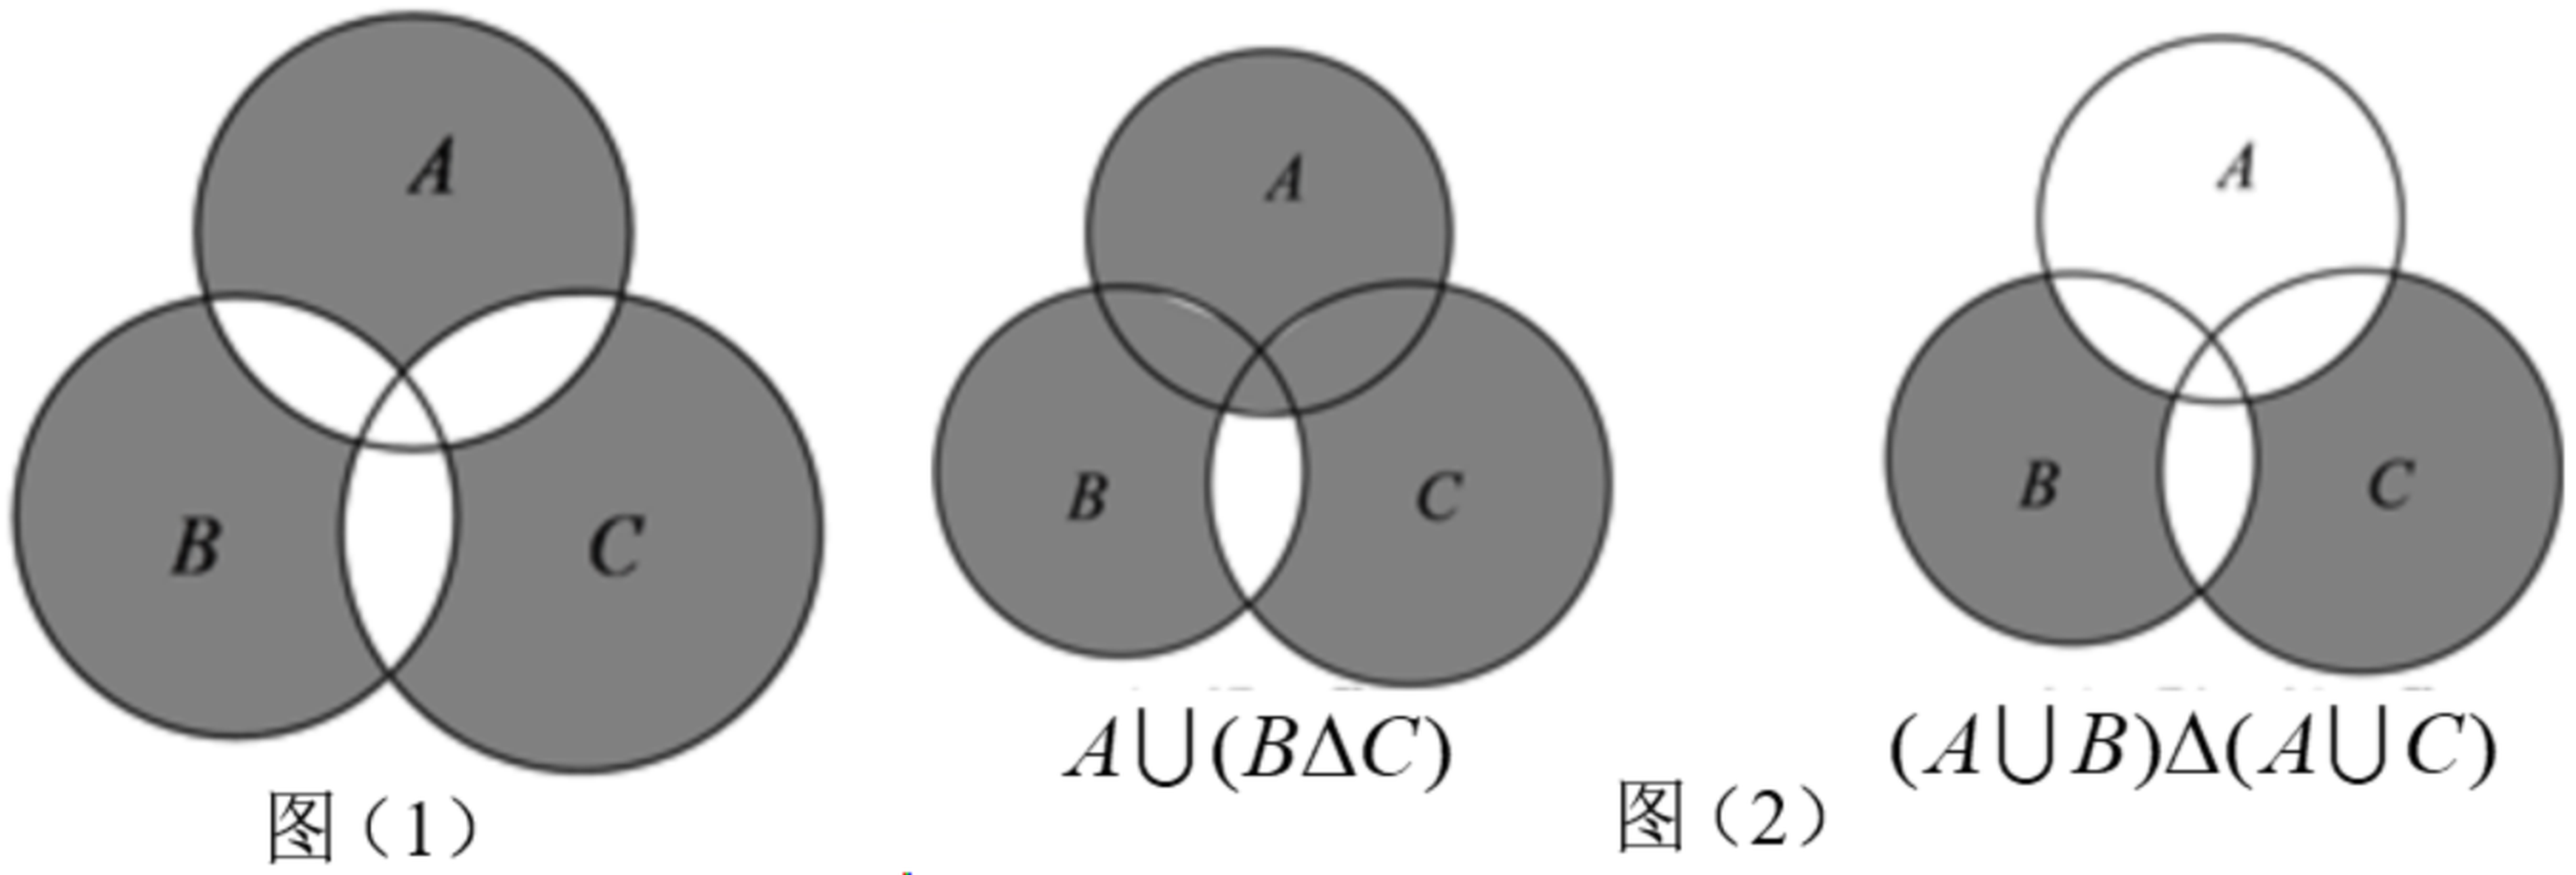
\includegraphics[width=0.86\textwidth]{figures/venn_symdiff3.png}
\end{center}

\step{对于③，由 $A\cap(B\Delta C)=A\cap(B\cup C-B\cap C)
=A\cap(B\cup C)-A\cap(B\cap C)$}
\step{$=(A\cap B)\cup(A\cap C)-(A\cap B)\cap(A\cap C)=(A\cap B)\Delta(A\cap C)$，
所以③正确；}
\step{对于④，如图（2）所示，$A\cup(B\Delta C)\neq(A\cup B)\Delta(A\cup C)$，
所以④错误.}
\step{故选 $B$.}
\solend

\fi

\end{enumerate}

\bigsec{三、解答题}

\begin{enumerate}
\setcounter{enumi}{16}

\item 已知集合 $M=\{x\mid a-1\leqslant x\leqslant2a+3\}$，$P=\{x\mid-2<x\leqslant4\}$，
全集 $U=\R$.

\begin{enumerate}[label=(\arabic*)]
\item 当 $a=2$ 时，求 $M\cap P$；
\item 若 $x\in P$ 是 $x\in M$ 的必要不充分条件，求实数 $a$ 的取值范围.
\end{enumerate}

\ifanswer
\solbegin
\stepm{(1)}{当 $a=2$ 时，集合 $M=\{x\mid1\leqslant x\leqslant7\}$，}
\step{所以 $M\cap P=\{x\mid1\leqslant x\leqslant4\}$；}
\stepm{(2)}{因为 $x\in P$ 是 $x\in M$ 的必要不充分条件，所以 $M\subset P$，}
\step{当 $M=\varnothing$ 时，$a-1>2a+3$，解得 $a<-4$，}
\step{当 $M\neq\varnothing$ 时，则
$\begin{cases}a-1\leqslant2a+3\\ a-1>-2\\ 2a+3\leqslant4\end{cases}$，
解得 $-1<a\leqslant\dfrac12$，}
\step{综上所述，实数 $a$ 的取值范围为
$(-\infty,-4)\cup\left(-1,\dfrac12\right]$.}
\solend

\fi

\ansspace[6]

\item 一辆汽车在某段路程中的行驶速度与时间的关系如图：

\begin{center}
% 图取原卷截图、4× LANCZOS 放大（速度—时间图：纵轴 $v/(\mathrm{km/h})$、
% 横轴 $t(\mathrm{h})$，$t\in[0,1]$、$[1,2]$、$[2,3]$ 三段矩形条高 50、80、90）。
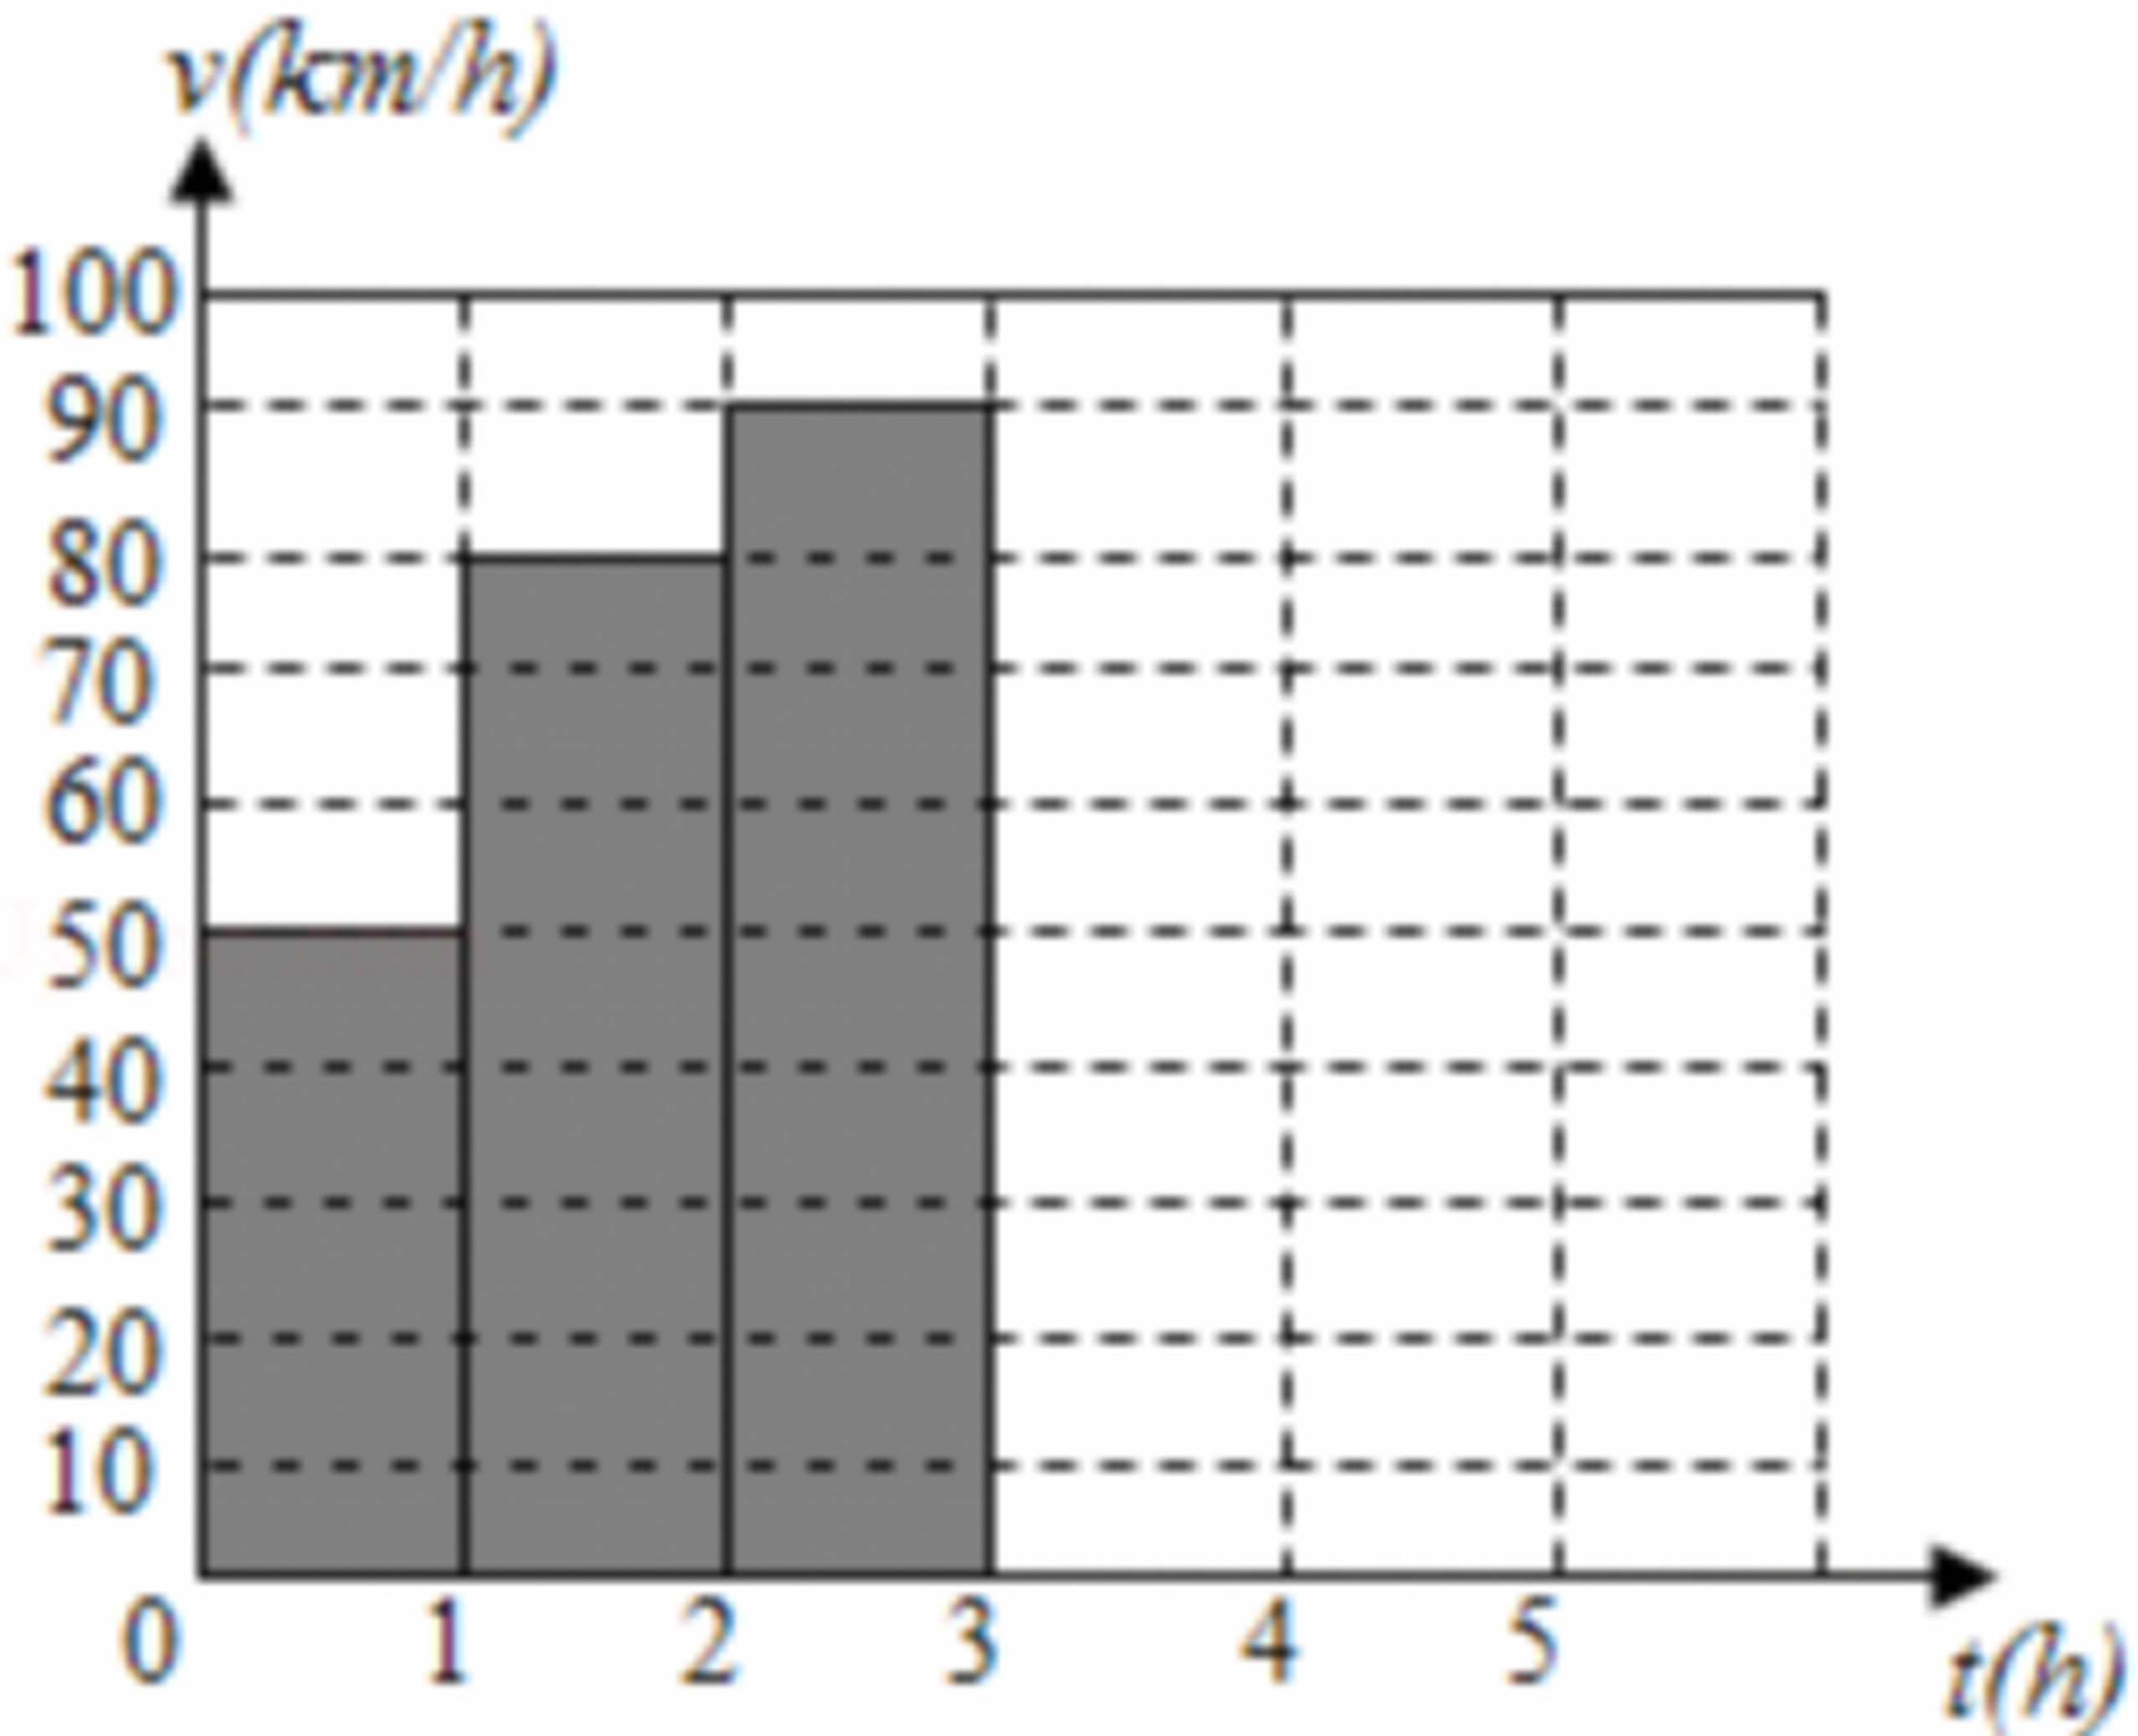
\includegraphics[width=0.52\textwidth]{figures/speed_time_bars.png}
\end{center}

\begin{enumerate}[label=(\arabic*)]
\item 求图中阴影部分的面积，并说明所求面积的实际意义；
\item 假设这辆汽车的里程表在汽车行驶这段路程前的读数为 $2004\,\mathrm{km}$，
试将汽车行驶这段路程时汽车里程表读数 $S$ 表示为时间 $t$ 的函数，
并求出当汽车里程表读数为 $2094\,\mathrm{km}$ 时，汽车行驶了多少时间？
\end{enumerate}

\ifanswer
\solbegin
\stepm{(1)}{由一辆汽车在某段路程中的行驶速度与时间的关系图，}
\step{得阴影部分的面积为 $50\times1+80\times1+90\times1=220$，}
\step{阴影部分的面积表示汽车在 $3$ 小时内行驶的路程为 $220\,\mathrm{km}$.}
\stepm{(2)}{$S=\begin{cases}
50t+2004,&0\leqslant t<1\\
80(t-1)+2054,&1\leqslant t<2\\
90(t-2)+2134,&2\leqslant t\leqslant3
\end{cases}$}
\step{令 $80(t-1)+2054=2094$，解得 $t=1.5$，所以汽车行驶 $1.5$ 小时.}
\solend

\fi

\ansspace[6]

\item 已知集合 $A=\{x\mid x<-2\text{ 或 }x\geqslant3\}$，$U=\R$.

\begin{enumerate}[label=(\arabic*)]
\item 求 $\overline{A}$；
\item 若 $B=\{x\mid mx-1>0\}$，当 $B\sub A$ 时，求实数 $m$ 的取值范围；
\item 若 $B=\{x\mid2m-6\leqslant x\leqslant m+4\}$，当 $B\cap\overline{A}=\varnothing$ 时，
求实数 $m$ 的取值范围.
\end{enumerate}

\ifanswer
\solbegin
\stepm{(1)}{因为集合 $A=\{x\mid x<-2\text{ 或 }x\geqslant3\}$，$U=\R$，
所以 $\overline{A}=\{x\mid-2\leqslant x<3\}$；}
\stepm{(2)}{当 $m=0$ 时，$B=\varnothing$，符合题意，}
\step{当 $m>0$ 时，$B=\left\{x\mid x>\dfrac1m\right\}$，则 $\dfrac1m\geqslant3$，
解得 $0<m\leqslant\dfrac13$，}
\step{当 $m<0$ 时，$B=\left\{x\mid x<\dfrac1m\right\}$，则 $\dfrac1m\leqslant-2$，
解得 $-\dfrac12\leqslant m<0$，}
\step{综上所述，实数 $m$ 的取值范围 $\left[-\dfrac12,\dfrac13\right]$；}
\stepm{(3)}{由题意得 $B=\{x\mid2m-6\leqslant x\leqslant m+4\}$，
$\overline{A}=\{x\mid-2\leqslant x<3\}$，且 $B\cap\overline{A}=\varnothing$，}
\step{当 $B=\varnothing$ 时，$2m-6>m+4$，解得 $m>10$，}
\step{当 $B\neq\varnothing$ 时，则 $\begin{cases}2m-6\leqslant m+4\\ m+4<-2\end{cases}$
或 $\begin{cases}2m-6\leqslant m+4\\ 2m-6\geqslant3\end{cases}$，}
\step{解得 $m<-6$ 或 $\dfrac92\leqslant m\leqslant10$，}
\step{综上所述，实数 $m$ 的取值范围为
$(-\infty,-6)\cup\left[\dfrac92,+\infty\right)$.}
\solend

\fi

\ansspace[8]

\item 在等腰梯形 $ABCD$ 中，$AB=DC=5$，$AD=4$，$BC=10$. 点 $E$ 在下底边 $BC$ 上.
点 $F$ 在腰 $AB$ 上.

\begin{center}
% 图取原卷截图、4× LANCZOS 放大（等腰梯形 $ABCD$ 与线段 $FE$，无辅助线）。
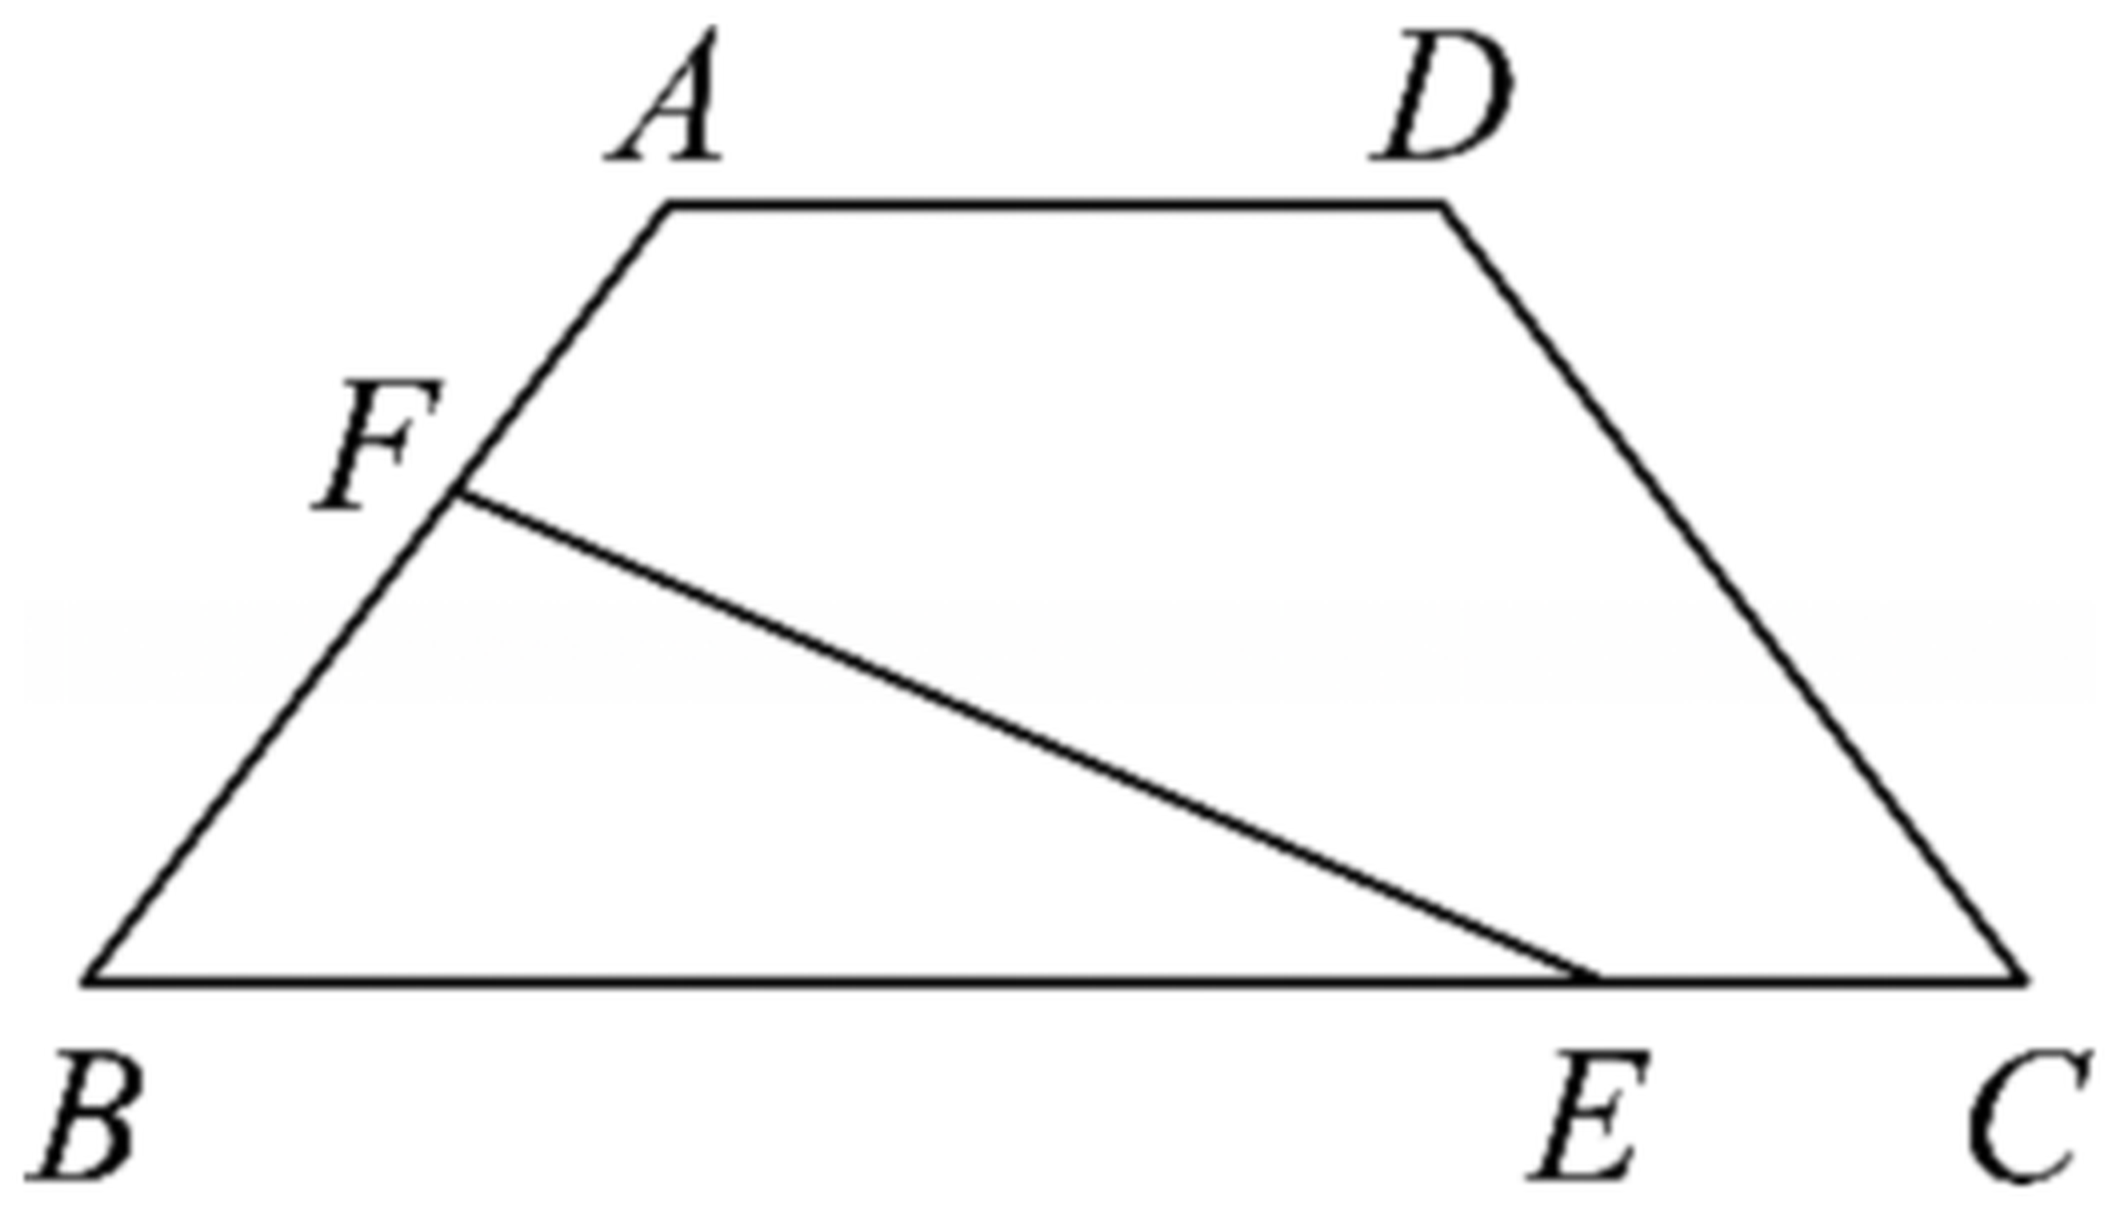
\includegraphics[width=0.46\textwidth]{figures/trapezoid_EF.png}
\end{center}

\begin{enumerate}[label=(\arabic*)]
\item 若 $EF$ 平分等腰梯形 $ABCD$ 的周长，设 $BE$ 长为 $x$，试用含 $x$ 的代数式表示
$\triangle BEF$ 的面积；
\item 是否存在线段 $EF$ 将等腰梯形 $ABCD$ 的周长和面积同时平分？若存在，求出此时 $BE$
的长；若不存在，请说明理由；
\item 是否存在线段 $EF$ 将等腰梯形 $ABCD$ 的周长和面积同时分成 $1:2$ 的两部分？
若存在，求此时 $BE$ 的长；若不存在，请说明理由.
\end{enumerate}

\ifanswer
\solbegin
\stepm{(1)}{过 $A$ 作 $AK\perp BC$ 交 $BC$ 于点 $K$，过 $F$ 作 $FG\perp BC$ 交 $BC$ 于点
$G$，}

\begin{center}
% 图取原卷截图、4× LANCZOS 放大（同梯形，多出虚线 $FG\perp BC$ 与 $AK\perp BC$
% 及两处直角符号；图只在【解析】里出现，故放进 \ifanswer 块）。
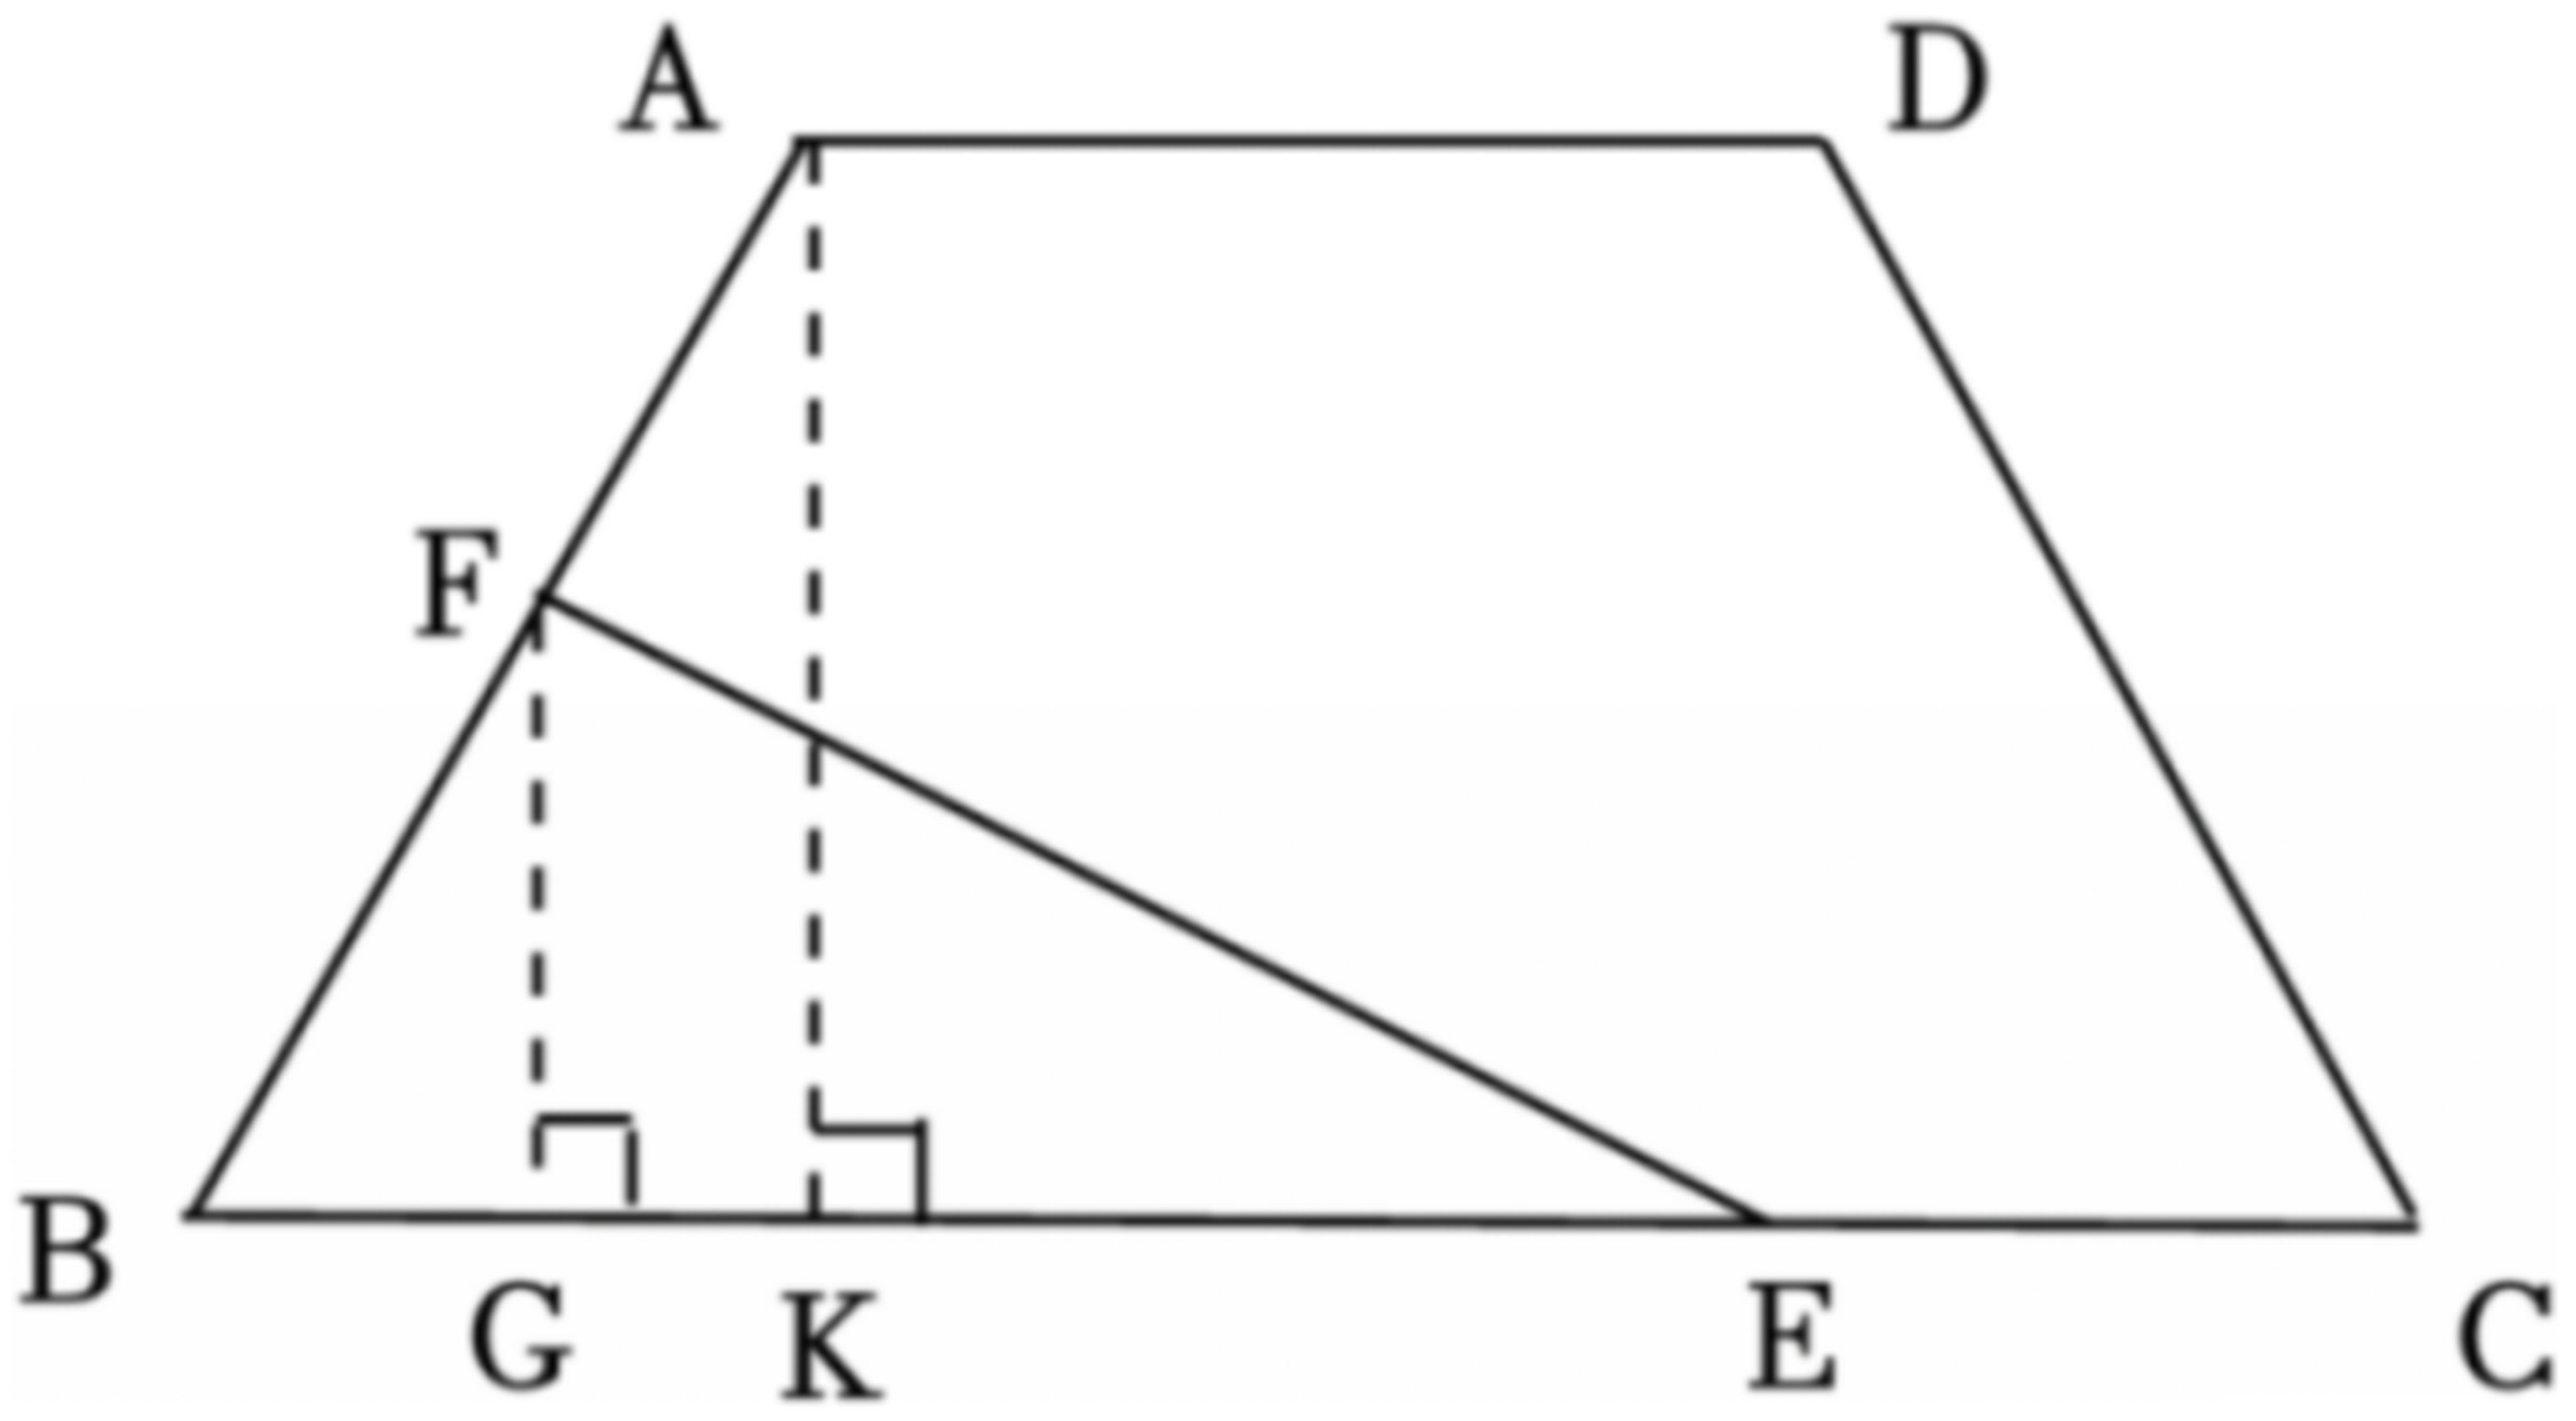
\includegraphics[width=0.62\textwidth]{figures/trapezoid_EF_aux.png}
\end{center}

\step{所以 $BK=\dfrac12\times(BC-AD)=\dfrac12\times(10-4)=3$，}
\step{$AK=\sqrt{AB^2-BK^2}=\sqrt{5^2-3^2}=4$，}
\step{由题意得，梯形 $ABCD$ 周长为 $24$，高为 $4$，面积为 $28$，}
\step{因为 $EF$ 平分等腰梯形 $ABCD$ 的周长，设 $BE$ 长为 $x$，则 $BF=12-x$，}
\step{由 $\begin{cases}0\leqslant12-x\leqslant5\\ 0\leqslant x\leqslant10\end{cases}$，
解得 $7\leqslant x\leqslant10$，}
\step{由题意得 $\triangle BFG\backsim\triangle BAK$，所以 $\dfrac{FG}{AK}=\dfrac{BF}{BA}$，
即 $\dfrac{FG}4=\dfrac{12-x}5$，}
\step{解得 $FG=\dfrac45(12-x)$，}
\step{所以 $S_{\triangle BEF}=\dfrac12BE\cdot FG
=-\dfrac25x^2+\dfrac{24}5x$（$7\leqslant x\leqslant10$）；}
\stepm{(2)}{存在，由 (1) 得 $-\dfrac25x^2+\dfrac{24}5x=\dfrac{28}2$，$x\in[7,10]$，}
\step{即 $x^2-12x+35=0$，解得 $x=7$ 或 $x=5$（舍去），}
\step{所以存在线段 $EF$ 将等腰梯形 $ABCD$ 的周长和面积同时平分，此时 $BE=7$；}
\stepm{(3)}{不存在，}
\step{情况一：$\triangle BEF$ 的面积$:$多边形 $AFECD$ 的面积 $=1:2$，
$(BE+BF):(AF+AD+DC+CE)=1:2$，}
\step{梯形周长的 $\dfrac13$ 是 $\dfrac{24}3=8$，面积的 $\dfrac13$ 是 $\dfrac{28}3$，}
\step{又因为 $BE=x$，所以 $BF=8-x$，}
\step{又因为 $\dfrac{FG}{AK}=\dfrac{BF}{BA}$，即 $\dfrac{FG}4=\dfrac{8-x}5$，
所以 $FG=\dfrac{32-4x}5$，}
\step{所以 $S_{\triangle BEF}=\dfrac12BE\times FG=-\dfrac25x^2+\dfrac{16}5x$，
所以 $\dfrac{28}3=-\dfrac25x^2+\dfrac{16}5x$，}
\step{整理得 $-3x^2+24x-70=0$，此时 $\Delta<0$，无解，故不存在；}
\step{情况二：$\triangle BEF$ 的面积$:$多边形 $AFECD$ 的面积 $=2:1$，
$(BE+BF):(AF+AD+DC+CE)=2:1$，}
\step{梯形周长的 $\dfrac13$ 为 $\dfrac{24}3=8$，面积的 $\dfrac13$ 为 $\dfrac{28}3$，
又 $BE=x$，所以 $BF=16-x$，}
\step{又 $\dfrac{FG}{AK}=\dfrac{BF}{BA}$，即 $\dfrac{FG}4=\dfrac{16-x}5$，
所以 $FG=\dfrac{64-4x}5$，}
\step{所以 $S_{\triangle BEF}=\dfrac12BE\times FG=-\dfrac25x^2+\dfrac{32}5x$，}
\step{所以 $\dfrac{28}3\times2=-\dfrac25x^2+\dfrac{32}5x$，
整理得 $-3x^2+48x-140=0$，}
\step{解得 $x=\dfrac{48+\sqrt{624}}6>10$，$x=\dfrac{48-\sqrt{624}}6<7$，
不符合题意，舍去，故不存在；}
\step{综上所述，不存在线段 $EF$ 将等腰梯形 $ABCD$ 的周长和面积同时分成 $1:2$ 的两部分.}
\solend

\fi

\ansspace[8]

\item 对集合 $\{1,2,\cdots,n\}$ 及其每一个非空子集 $A$，定义一个唯一确定的“交替和”
如下：将 $A$ 中的元素按照递减的次序排列，然后将第一个元素交替地减或加后继的元素所得的
结果，例如，子集 $\{1,2,4,6,9\}$ 的“交替和”是 $9-6+4-2+1=6$，子集 $\{5,6\}$ 的
“交替和”是 $6-5=1$，子集 $\{2\}$ 的交替和是 $2$；定义一个唯一确定的“交替积”如下：
将 $A$ 中的元素按照递减的次序排列，然后将第一个元素交替地除以或乘以后继的数所得的结果，
例如，集合 $\{1,2,4,6,9\}$ 的“交替积”是 $9\div6\times4\div2\times1=3$，
$\{5,6\}$ 的“交替积”是 $6\div5=1.2$，$\{2\}$ 的“交替积”是 $2$.

\begin{enumerate}[label=(\arabic*)]
\item 对于 $\{1,2,3,4,5,6,7,8,9\}$，求其所有子集的“交替和”的总和；
\item 对于 $\{1,2,\cdots,n\}$，求其所有子集的“交替和”的总和；
\item 对于 $\left\{n\mid\dfrac{495}{n+2}\in\N,n\in\Z\right\}$ 求其所有子集的
“交替积”的总和.
\end{enumerate}

\ifanswer
\solbegin
\stepm{(1)}{集合 $\{1,2,3,4,5,6,7,8,9\}$ 的子集中，除去 $\{9\}$ 外还有 $2^9-2$ 个
非空子集，}
\step{把这 $2^9-2$ 个非空子集两两组合后分别计算每一组中“交替和”之和，}
\step{组合原则是设 $A_i=\{9,a_1,a_2,\cdots\}$，$A_i^1=\{a_1,a_2,\cdots\}$，}
\step{集合 $A_i^1$ 的元素为集合 $A_i$ 中去掉 $9$ 的所有元素，把 $A_i$ 和 $A_i^1$
结合为一组，}
\step{显然，每组的“交替和”的和为 $9$，共有 $\dfrac{2^9-2}2$ 组，}
\step{所以，所有“交替和”之和应该为 $\dfrac{9(2^9-2)}2+9=2304$；}
\stepm{(2)}{集合 $\{1,2,\cdots,n\}$ 的子集中，除去 $\{n\}$ 外还有 $2^n-2$ 个非空子集，}
\step{把这 $2^n-2$ 个非空子集两两组合后分别计算每一组中“交替和”之和，}
\step{组合原则是设 $A_i=\{n,a_1,a_2,\cdots\}$，$A_i^1=\{a_1,a_2,\cdots\}$，}
\step{集合 $A_i^1$ 的元素为集合 $A_i$ 中去掉 $n$ 的所有元素，把 $A_i$ 和 $A_i^1$
结合为一组，}
\step{显然，每组的“交替和”的和为 $n$，共有 $\dfrac{2^n-2}2$ 组，}
% 注：下一行分子原卷印作花括号（其余同类处皆用圆括号），照抄未改，见文件头“原卷存疑”③。
\step{所以，所有“交替和”之和应该为 $\dfrac{n\{2^n-2\}}2+n=n\cdot2^{n-1}$；}
\stepm{(3)}{集合 $\left\{n\mid\dfrac{495}{n+2}\in\N,n\in\Z\right\}
=\{493,163,97,53,43,31,13,9,7,3,1,-1\}$，}
\step{其中除去 $\{-1\}$ 外还有 $2^{12}-2$ 个非空子集，}
% 注：下一行原卷把“把这”重复印了一次（“把这把这”），照抄未改，见文件头“原卷存疑”②。
\step{把这把这 $2^{12}-2$ 个非空子集两两组合后分别计算每一组中“交替积”之和，}
\step{组合原则是设 $A_j=\{-1,a_1,a_2,\cdots\}$，$A_j^1=\{a_1,a_2,\cdots\}$，}
\step{集合 $A_j^1$ 的元素为集合 $A_j$ 中去掉 $-1$ 的所有元素，把 $A_j$ 和 $A_j^1$
结合为一组，}
\step{显然，每组的“交替积”的和为 $0$，共有 $\dfrac{2^{12}-2}2$ 组，}
\step{所以，所有“交替积”之和应该为 $\dfrac{2^{12}-2}2\times0-1=-1$.}
\solend

\fi

\ansspace*[10]

\end{enumerate}

\end{document}
"
%
% 原始材料是微信公众号图文（公众号“魔都数学加油站”连载“27学年高一 30”，2026-09-23 发布，
% 原文标题“27学年高一30——2026-2027年上海市南洋模范中学高一上开学考”），
% 正文为 11 张 PNG 页。**同一篇里各页分辨率不一致**——第 2、3、9、10 页 4762×6735，
% 其余七页 2560×3620（已逐页打开确认，非下载缺档），取的是 mmbiz.qpic.cn/<hash>/0 的原图档。
% 原文本身就是一份**讲评版**：填空第 3—7 题下方印【答案】，第 8—12 题与其后各题印【解析】。
% 试题文字、答案与解析均照原卷录入，未改内容。卷面的粉色斜水印属水印，未录入。
%
% 卷首标题：原卷印作“2026-2027 年南洋模范中学高一上开学考”（公众号标题里的“上海市”
% 三字卷面标题行没有，本稿照卷面），年份区间按全稿惯例排 en dash，前缀照原卷保留“年”。
%
% 与原卷的排版差异（均已在 README“说明”中交代）：
%   ① 原文自**第 3 题**起（第 1、2 题未在该文中发布），故本稿题号亦自 3 起；
%   ② 原卷本就印有“一、填空题”“二、选择题”“三、解答题”三节标题，本稿照原卷分节，
%      只把标题改排成全稿统一的“大节标题”样式；
%   ③ 原卷填空第 3—7 题只印【答案】行、第 8 题起印【解析】（选择题答案写在解析末句
%      “故选 D／B”里），本稿统一改为试卷版隐去、答案版以 \ans{}／\ifanswer 块给出，
%      两版彻底分离；
%   ④ 子集符号原卷两种并用：第 7 题题干两处、第 19(2) 题作带下划线的 $\subseteq$，
%      第 17(2) 题解析作真包含的 $\subset$，本稿分别照录为 $\sub$ 与 $\subset$；
%   ⑤ 补集符号原卷一律作**上横线**（$\overline{A}$、$\overline{B}$），本稿照录；
%   ⑥ 原卷的实数集 R 一律作斜体（第 4 题、第 17 题与第 19 题题干的 $U=R$），
%      第 21(3) 题的自然数集与整数集作**粗体** $\mathbf{N}$、$\mathbf{Z}$，
%      本稿按全稿惯例统一写作 $\R$、$\N$、$\Z$；
%   ⑦ 原卷填空的横线约两个字宽，本稿按全稿惯例统一排 \blankline[4.4em]；
%   ⑧ 原卷未印副标题，本稿按全稿惯例补出副标题“集合与常用逻辑用语”——但本卷是开学考，
%      范围不止这一章：第 18 题是速度—时间图象题、第 20 题是等腰梯形的周长/面积平分问题，
%      副标题只标了主章节（见文末“高一30 专记”）；
%   ⑨ 第 13、14、18、20 题的图印在题干右侧、第 16 题的三幅图印在【解析】里的下一页顶部、
%      第 20 题【解析】另有一张带辅助线的图，本稿一律移至题干或解析之后；
%      图取原卷截图、4× LANCZOS 放大（见各 \includegraphics 前的注释）。
%
% 原卷存疑三处（均照抄原卷、未改，见源码中该处上方注释）：
%   ① 第 10 题【解析】验证“破晓集”时写的是 $\notin A$、$\in A$（如“$-2-2=-4\notin A$”），
%      但该处讨论的集合原题设里叫 $P$，同题②的“$x+y=2(k_1+k_2)\in A$”亦然——
%      本稿照抄未改（按文意应为 $P$）；
%   ② 第 21 题【解析】(3) 有“把这把这 $2^{12}-2$ 个非空子集”（“把这”重复印了一次）；
%   ③ 同题 (2) 的结论式分子原卷印作花括号 $\dfrac{n\{2^n-2\}}{2}$（其余同类处皆用圆括号）。

\documentclass[a4paper,11pt]{article}
\usepackage{common}

\begin{document}

\examtitlest[3]{2026--2027 年南洋模范中学高一上开学考}{集合与常用逻辑用语}

\bigsec{一、填空题}

\begin{enumerate}
\setcounter{enumi}{2}

\item 若集合 $A=\{x\mid x^2-2kx+7k=0\}$ 有且仅有三个真子集，则 $k$ 的取值范围是
\blankline[4.4em].

\ans{$(-\infty,0)\cup(7,+\infty)$}

\item “存在 $x\in\R$，使得 $x^2+2x+5=0$”的否定形式是 \blankline[4.4em].

\ans{对任何 $x\in\R$，都有 $x^2+2x+5\neq0$}

\item 下列命题中，$p$ 是 $q$ 的必要非充分条件的是 \blankline[4.4em].

① $p:x>2$ 且 $y>3$，$q:x+y>5$；

② $p$：四边形的四个角都相等，$q$：四边形是正方形.

\ans{②}

\item 若“条件 $\alpha:2\leqslant x\leqslant4$”是“条件 $\beta:3m-1\leqslant x\leqslant-m$”的
充分非必要条件，则 $m$ 的取值范围是 \blankline[4.4em].

\ans{$(-\infty,-4]$}

\item 满足 $\{1\}\sub M\sub\{1,2,4,5\}$ 的集合 $M$ 的个数为 \blankline[4.4em] 个.

\ans{$8$}

\item 已知集合 $A=\{1,2\}$，集合 $B=\{x\mid ax=6\}$，若 $A\cup B=A$，则 $a$ 的所有取值
构成的集合为 \blankline[4.4em].

\ifanswer
\solbegin
\step{因为 $A\cup B=A$，所以 $B\sub A$，}
\step{当 $a=0$ 时，$B=\varnothing$，满足 $B\sub A$；}
\step{当 $a\neq0$ 时，$B=\left\{\dfrac6a\right\}$，则 $\dfrac6a=1$ 或 $\dfrac6a=2$，
解得 $a=6$ 或 $a=3$，}
\step{综上所述，$a$ 的所有取值构成的集合为 $\{0,3,6\}$.}
\solend

\fi

\item 对于集合 $M$、$N$，定义 $M-N=\{x\mid x\in M\text{ 且 }x\notin N\}$，
$M\oplus N=(M-N)\cup(N-M)$，设 $A=\{y\mid y=|x|,x\in\R\}$，
$B=\{y\mid y=-(x-1)^2+2,x\in\R\}$，则 $A\oplus B=$ \blankline[4.4em].

\ifanswer
\solbegin
\step{由已知 $A=[0,+\infty)$，$B=(-\infty,2]$，}
\step{由于 $A-B=(2,+\infty)$，$B-A=(-\infty,0)$，}
\step{故 $A\oplus B=(A-B)\cup(B-A)=(-\infty,0)\cup(2,+\infty)$.}
\solend

\fi

\item 设 $P$ 为非空实数集满足：对任意给定的 $x$、$y\in P$（$x$、$y$ 可以相同），都有
$x+y\in P$，$x-y\in P$，$xy\in P$，则称 $P$ 为破晓集. 关于破晓集有下列结论：
①集合 $P=\{-2,-1,0,1,2\}$ 为破晓集；②集合 $P=\{x\mid x=2n,n\in\Z\}$ 为破晓集；
③若集合 $P_1$、$P_2$ 为破晓集，则 $P_1\cup P_2$ 为破晓集；④若集合 $P$ 为破晓集，
则一定有 $0\in P$；⑤若集合 $P_1$、$P_2$ 为破晓集，则 $P_1\cap P_2$ 为破晓集；
其中正确结论的序号是 \blankline[4.4em].

\ifanswer
\solbegin
% 注：以下几步原卷把该集合记作 $A$（题设里叫 $P$），照抄未改，见文件头“原卷存疑”①。
\step{对于①：$-2-2=-4\notin A$，故集合 $P=\{-2,-1,0,1,2\}$ 不为破晓集，故①错误；}
\step{②设 $x$、$y\in A$，则 $x=2k_1$，$y=2k_2$，且 $k_1$、$k_2\in\Z$，}
\step{故 $x+y=2(k_1+k_2)\in A$，$x-y=2(k_1-k_2)\in A$，$xy=4k_1k_2\in A$，}
\step{故集合 $P=\{x\mid x=2n,n\in\Z\}$ 为破晓集，故②正确；}
\step{③若集合 $P_1$、$P_2$ 为破晓集，设 $P_1=\{x\mid x=2k,k\in\Z\}$，
$P_2=\{x\mid x=3k,k\in\Z\}$，}
\step{但是 $P_1\cup P_2$ 不为破晓集，如 $x=2$，$y=3$ 时，$x+y=5$，
故 $5\notin(P_1\cup P_2)$，故③错误；}
\step{④若集合 $P$ 为破晓集，则取 $x=y$，$x-y=0\in A$，则一定有 $0\in P$，故④正确.}
\step{⑤正确；}
\step{故正确的是②④⑤.}
\solend

\fi

\item 已知集合 $M$ 的元素均为正整数，定义集合 $M$ 的“变项和”为：将 $M$ 中每个元素 $m$
都乘以 $(-1)^m$ 后再求和. 若集合 $A=\{n\mid1\leqslant n\leqslant10,n\in\N\}$，则集合 $A$
的所有非空子集的“变项和”的总和为 \blankline[4.4em].

\ifanswer
\solbegin
\step{$A$ 集合的所有非空子集中，每个元素出现的次数都是
$(2^{10}-1)-(2^9-1)=2^9$，}
\step{则集合 $A$ 的所有非空子集的“变项和”的总和为
$1\times(-1)^1\times2^9+2\times(-1)^2\times2^9+\cdots+10\times(-1)^{10}\times2^9$}
\step{$=(-1+2-3+4-\cdots-9+10)\times2^9=5\times2^9=2560$.}
\solend

\fi

\item 已知集合 $A=[t,t+1]\cup[t+4,t+9]$，$0\notin A$，存在正数 $\lambda$，使得对任意
$a\in A$，都有 $\dfrac\lambda a\in A$，则 $t$ 的值是 \blankline[4.4em].

\ifanswer
\solbegin
\step{当 $t>0$ 时，当 $a\in[t,t+1]$ 时，$\dfrac\lambda a\in[t+4,t+9]$，}
\step{当 $a\in[t+4,t+9]$ 时，$\dfrac\lambda a\in[t,t+1]$，}
\step{即当 $a=t$ 时，$\dfrac\lambda a\leqslant t+9$；当 $a=t+9$ 时，
$\dfrac\lambda a\geqslant t$，即 $\lambda=t(t+9)$；}
\step{当 $a=t+1$ 时，$\dfrac\lambda a\geqslant t+4$，当 $a=t+4$ 时，
$\dfrac\lambda a\leqslant t+1$，即 $\lambda=(t+1)(t+4)$，}
\step{所以 $t(t+9)=(t+1)(t+4)$，解得 $t=1$.}
\step{当 $t+1<0<t+4$ 时，当 $a\in[t,t+1]$ 时，$\dfrac\lambda a\in[t,t+1]$.}
\step{当 $a\in[t+4,t+9]$ 时，则 $\dfrac\lambda a\in[t+4,t+9]$，}
\step{即当 $a=t$ 时，$\dfrac\lambda a\leqslant t+1$，当 $a=t+1$ 时，
$\dfrac\lambda a\geqslant t$，即 $\lambda=t(t+1)$，}
\step{即当 $a=t+4$ 时，$\dfrac\lambda a\leqslant t+9$，当 $a=t+9$ 时，
$\dfrac\lambda a\geqslant t+4$，即 $\lambda=(t+4)(t+9)$，}
\step{所以 $t(t+1)=(t+4)(t+9)$，解得 $t=-3$.}
\step{当 $t+9<0$ 时，同理可得无解.}
\step{综上，$t$ 的值为 $1$ 或 $-3$.}
\solend

\fi

\end{enumerate}

\bigsec{二、选择题}

\begin{enumerate}
\setcounter{enumi}{12}

% 这道题是“题干 + 图 + 选项”约 6cm 的一整块，页末放不下就会被拆开（切页审计的 A 类），
% 故在题前先量一次页高：不够就把整道题干连图带选项一起挪到次页。
\needvspace{6.5cm}
\item 设 $U=\{1,2,3,4,5\}$，$A$、$B$ 都是 $U$ 的子集，且 $A\cap B=\{5\}$，
$\overline{A}\cap B=\{4\}$，$\overline{A}\cap\overline{B}=\{1,2\}$，
则以下四个判断中正确的是\mbox{（\quad）}

\begin{center}
% 图取原卷截图、4× LANCZOS 放大（原卷把图印在题干右侧，本稿移至此处，见文件头⑨）。
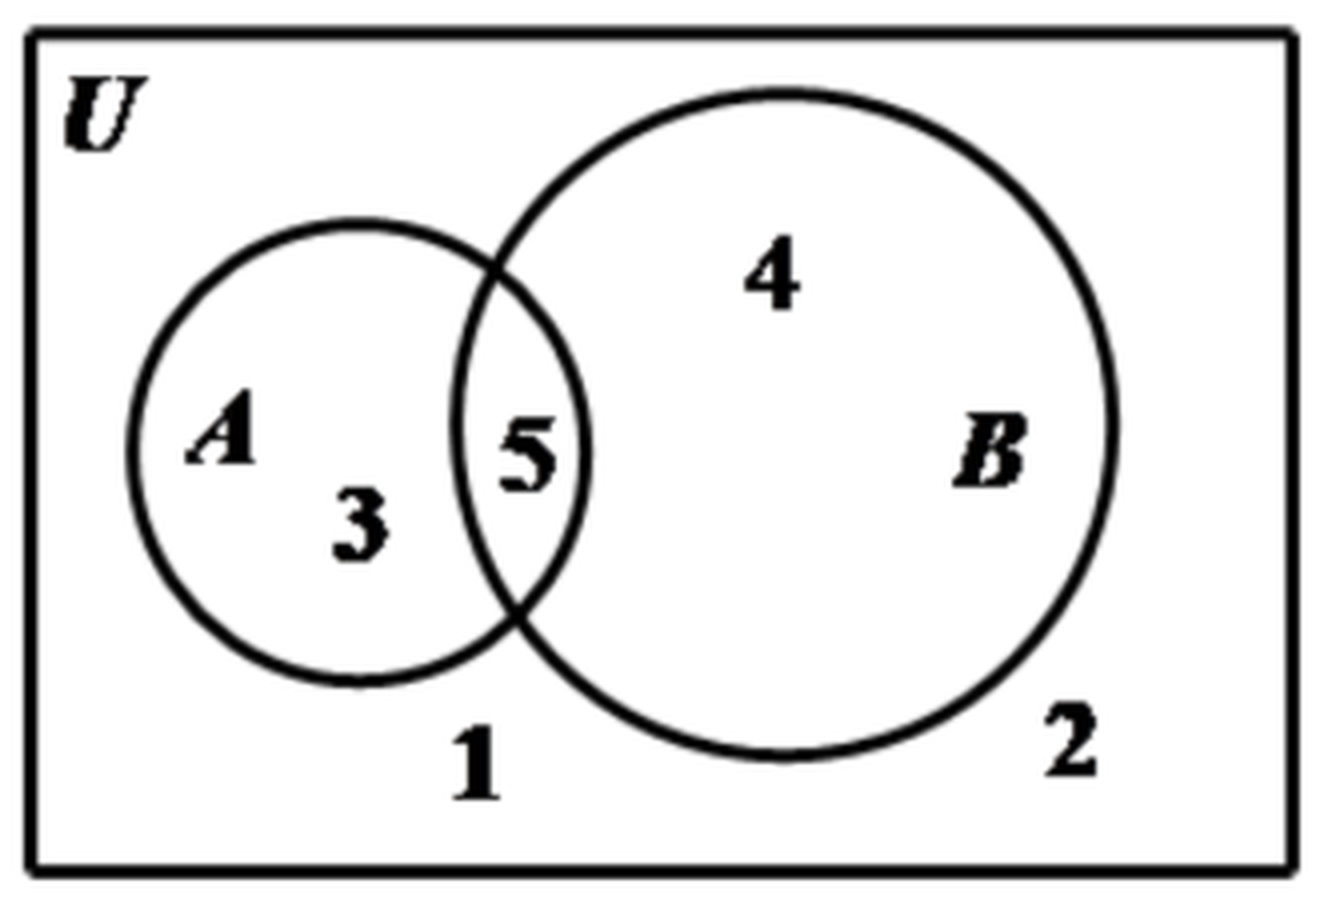
\includegraphics[width=0.28\textwidth]{figures/venn_U5_AB.png}
\end{center}

\keepwithprev
A. $3\notin A$ 且 $3\notin B$\qquad\qquad B. $3\in A$ 且 $3\in B$

C. $3\notin A$ 且 $3\in B$\qquad\qquad D. $3\in A$ 且 $3\notin B$

\ans{$D$}

\ifanswer
\solbegin
\step{画出韦恩图，得 $A=\{5,3\}$，$B=\{5,4\}$，}
\step{则 $3\in A$ 且 $3\notin B$. 故选 $D$.}
\solend

\fi

% 同第 13 题：整块（题干 + 图 + 选项）在答案版还要再挂【答案】【解析】，页末更易被拆开。
\needvspace{7.5cm}
\item 如图表示图形阴影部分的是\mbox{（\quad）}

\begin{center}
% 图取原卷截图、4× LANCZOS 放大（三圆 $A$、$B$、$C$，阴影为整个 $A$ 圆加 $B\cap C$）。
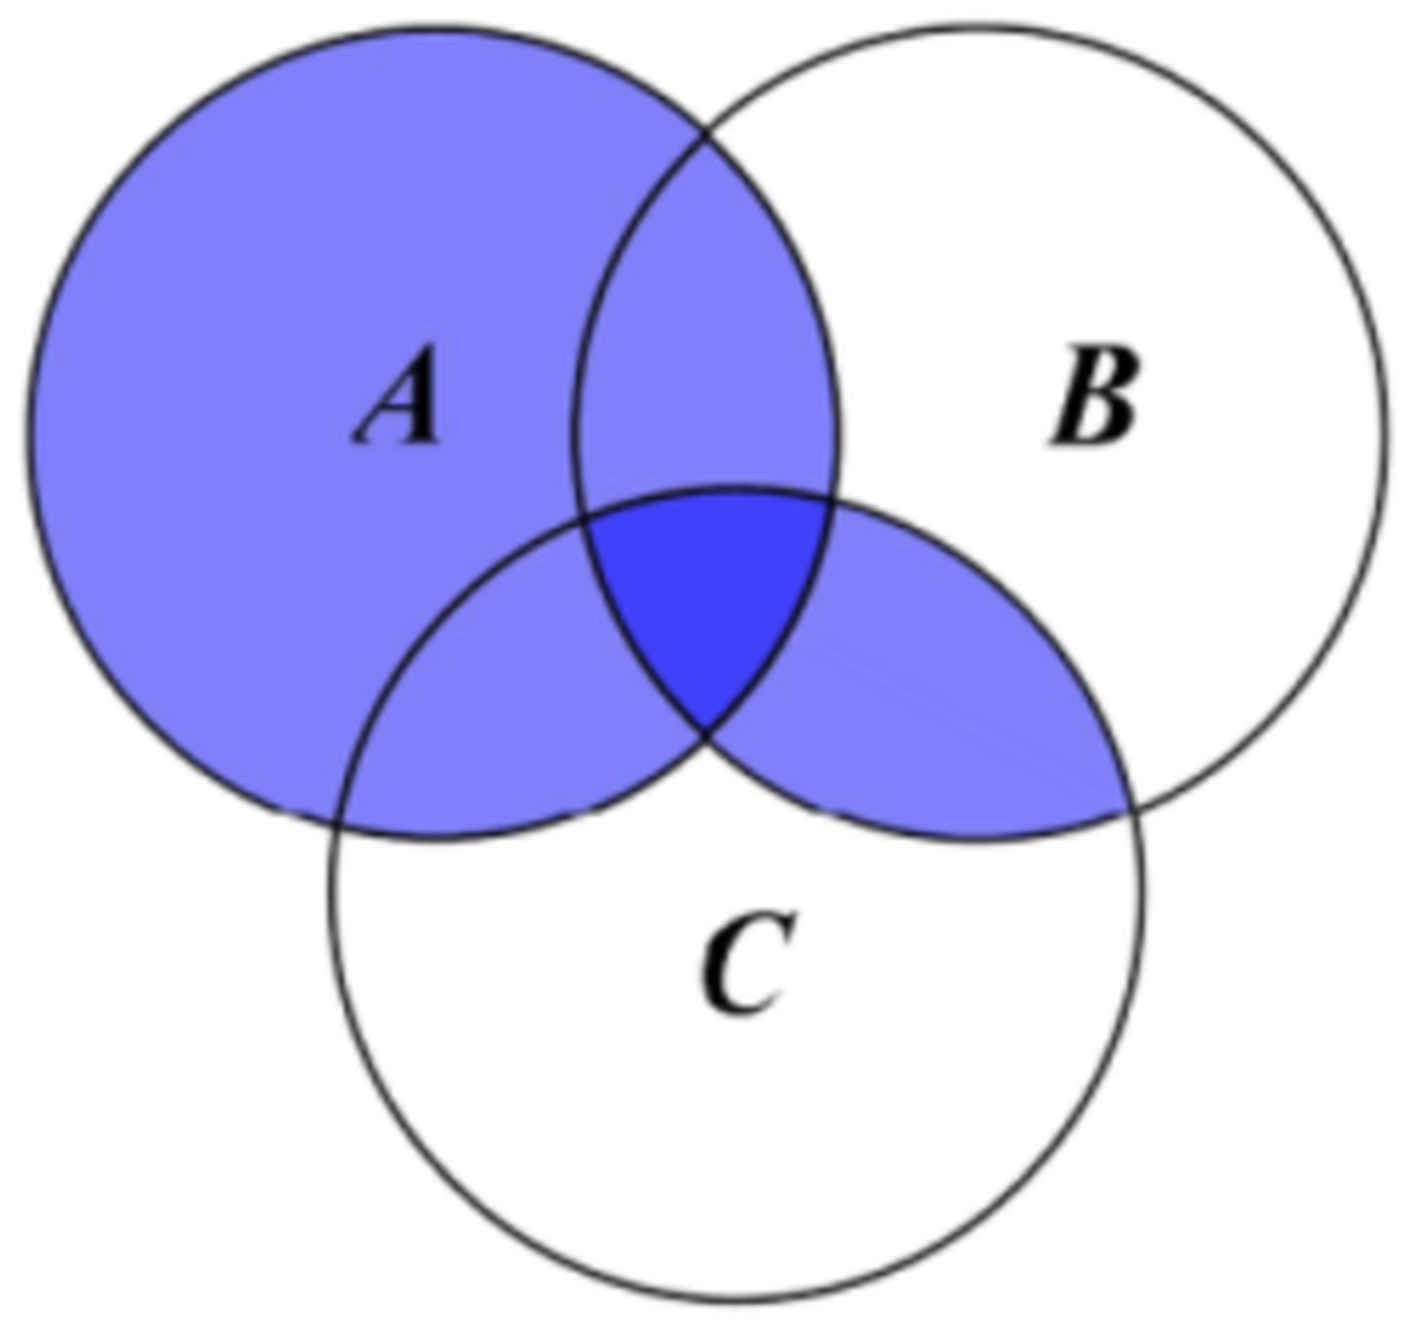
\includegraphics[width=0.30\textwidth]{figures/venn_A_union_BC.png}
\end{center}

\keepwithprev
A. $(A\cup C)\cap(B\cup C)$\qquad\qquad B. $(A\cup B)\cap(A\cup C)$

C. $(A\cup B)\cap(B\cup C)$\qquad\qquad D. $(A\cup B)\cap C$

\ans{$B$}

\ifanswer
\solbegin
\step{图中阴影部分表示元素满足是 $A$ 中的元素，或者是 $B$ 与 $C$ 的公共元素，}
\step{故可以表示为 $A\cup(B\cap C)$，也可以表示为 $(A\cup B)\cap(A\cup C)$.
故选 $B$.}
\solend

\fi

\item 设集合 $M=\left\{x\mid m\leqslant x\leqslant m+\dfrac34\right\}$，
$N=\left\{x\mid n-\dfrac13\leqslant x\leqslant n\right\}$，且 $M$、$N$ 都是集合
$\{x\mid0\leqslant x\leqslant1\}$ 的子集，如果把 $b-a$ 叫做集合
$\{x\mid a\leqslant x\leqslant b\}$ 的“长度”，那么集合 $M\cap N$ 的“长度”的
最小值是\mbox{（\quad）}

\keepwithprev
A. $\dfrac23$\qquad B. $\dfrac1{12}$\qquad C. $\dfrac13$\qquad D. $\dfrac5{12}$

\ans{$B$}

\ifanswer
\solbegin
\step{$M$ 的长度为 $\dfrac34$，$N$ 的长度为 $\dfrac13$，}
\step{当集合 $M\cap N$ 的长度的最小值时，$M$ 与 $N$ 应分别在区间 $[0,1]$ 的左右两端，}
\step{故 $M\cap N$ 的长度的最小值是 $\dfrac34+\dfrac13-1=\dfrac1{12}$，故选 $B$.}
\solend

\fi

\item 定义集合运算 $A-B=\{x\mid x\in A\text{ 且 }x\notin B\}$ 称为集合 $A$ 与集合 $B$ 的
差集；定义集合运算 $A\Delta B=(A-B)\cup(B-A)$ 称为集合 $A$ 与集合 $B$ 的对称差，
有以下 $4$ 个等式：① $A\Delta B=B\Delta A$；② $(A\Delta B)\Delta C=A\Delta(B\Delta C)$；
③ $A\cap(B\Delta C)=(A\cap B)\Delta(A\cap C)$；
④ $A\cup(B\Delta C)=(A\cup B)\Delta(A\cup C)$，
则 $4$ 个等式中恒成立的是\mbox{（\quad）}

\keepwithprev
A. ①②\qquad B. ①②③\qquad C. ①②④\qquad D. ①②③④

\ans{$B$}

\ifanswer
\solbegin
\step{对于①，由 $B\Delta A=(B-A)\cup(A-B)=(A-B)\cup(B-A)=A\Delta B$，
所以①正确；}
\step{对于②，由 $A-B=\{x\mid x\in A\text{ 且 }x\notin B\}
=\{x\mid x\in A,x\notin(A\cap B)\}=A-(A\cap B)$，}
\step{同理可得 $B-A=B-(A\cap B)$，}
\step{则 $A\Delta B=(A-B)\cup(B-A)=(A\cup B)-(A\cap B)$，}
\step{所以 $(A\Delta B)\Delta C=(A\Delta B)\cup C-(A\Delta B)\cap C$，}
\step{所以表示的集合为图（1）中阴影部分所表示的集合，如图所示，}
\step{同理 $A\Delta(B\Delta C)=A\cup(B\Delta C)-A\cap(B\Delta C)$，
也表示图（1）中阴影部分所表示的集合，}
\step{所以 $(A\Delta B)\Delta C=A\Delta(B\Delta C)$，所以②正确；}

\begin{center}
% 图取原卷截图、4× LANCZOS 放大（原卷印在下一页顶部，共三幅三圆韦恩图：
% 图（1）一幅、图（2）左右两幅，图（2）两幅下方各有一行式子标注）。
% 图只在【解析】里出现，故放进 \ifanswer 块，试卷版不排。
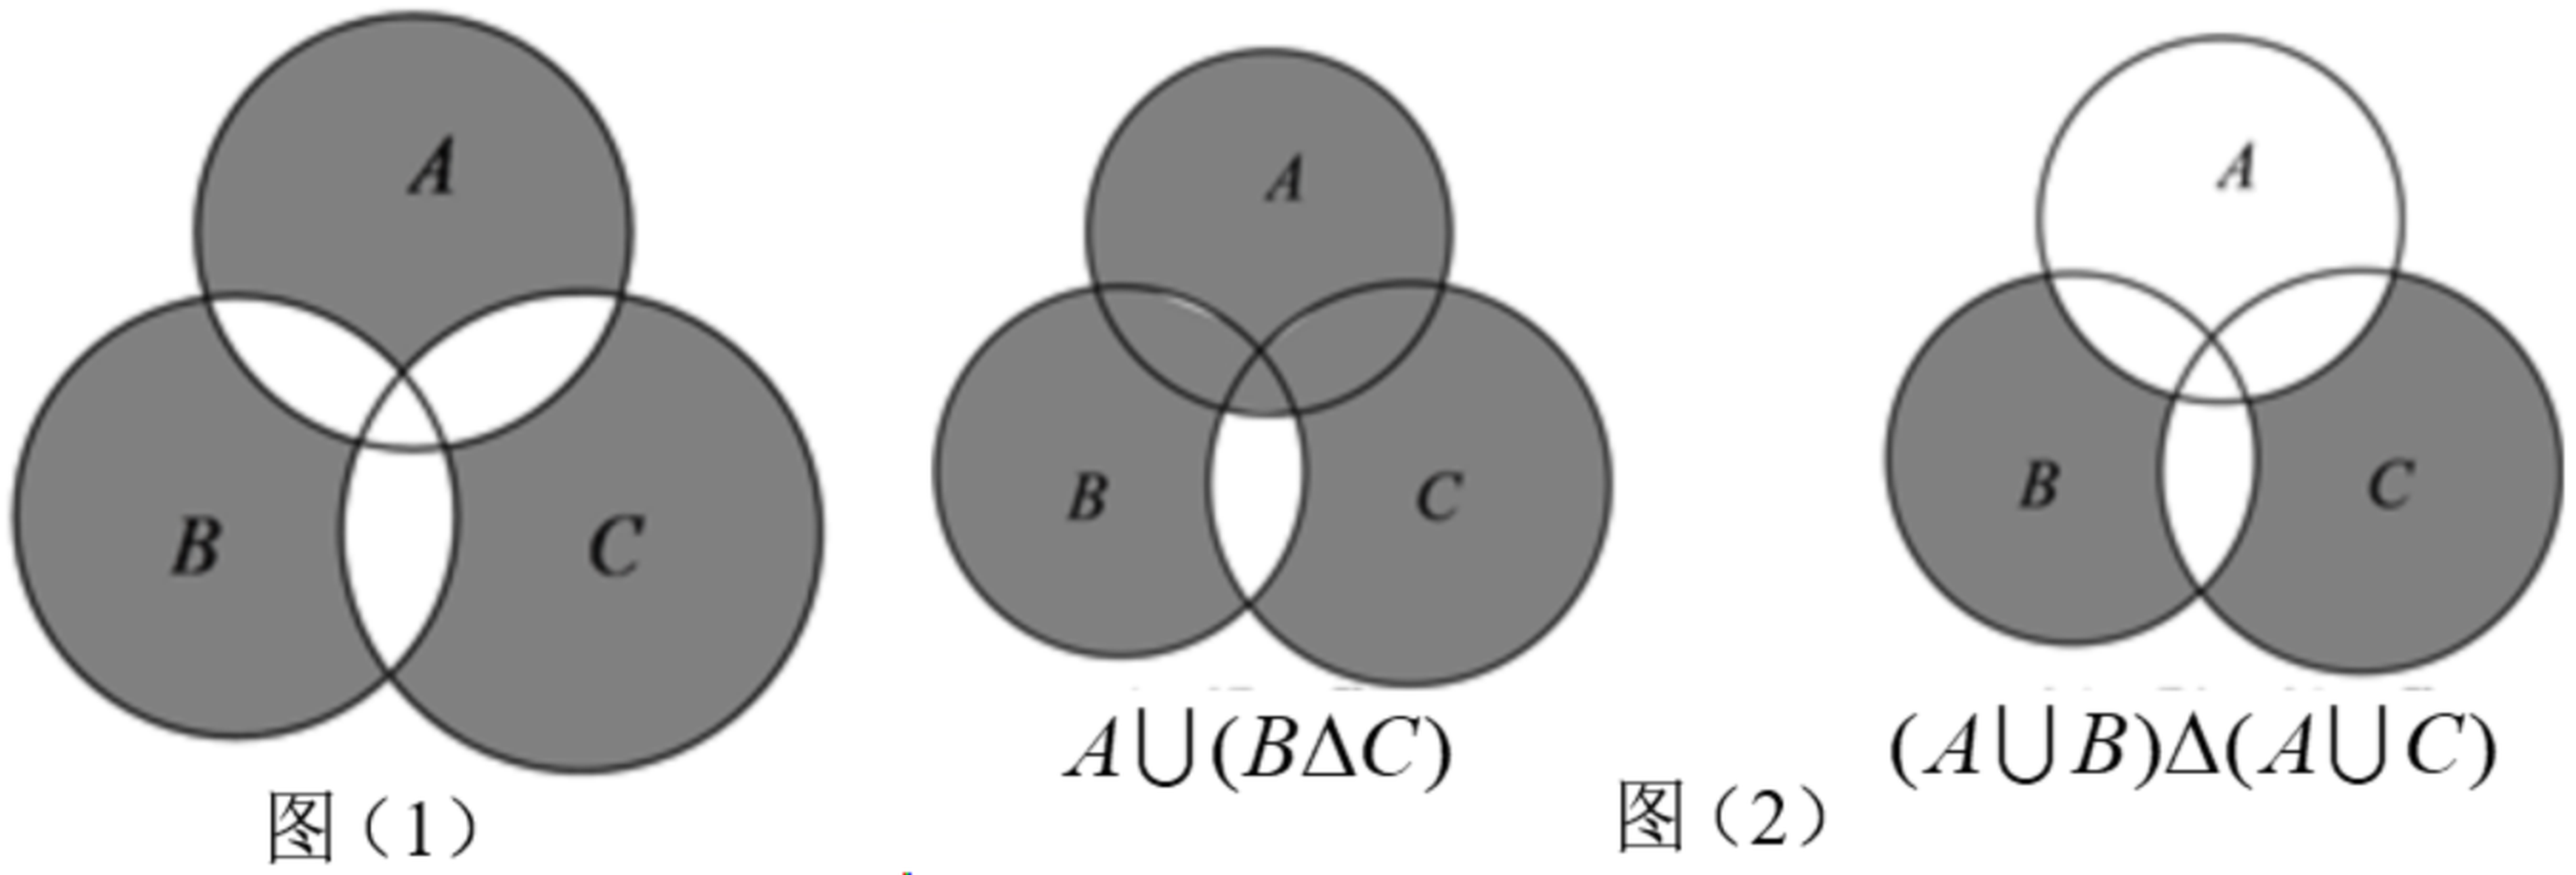
\includegraphics[width=0.86\textwidth]{figures/venn_symdiff3.png}
\end{center}

\step{对于③，由 $A\cap(B\Delta C)=A\cap(B\cup C-B\cap C)
=A\cap(B\cup C)-A\cap(B\cap C)$}
\step{$=(A\cap B)\cup(A\cap C)-(A\cap B)\cap(A\cap C)=(A\cap B)\Delta(A\cap C)$，
所以③正确；}
\step{对于④，如图（2）所示，$A\cup(B\Delta C)\neq(A\cup B)\Delta(A\cup C)$，
所以④错误.}
\step{故选 $B$.}
\solend

\fi

\end{enumerate}

\bigsec{三、解答题}

\begin{enumerate}
\setcounter{enumi}{16}

\item 已知集合 $M=\{x\mid a-1\leqslant x\leqslant2a+3\}$，$P=\{x\mid-2<x\leqslant4\}$，
全集 $U=\R$.

\begin{enumerate}[label=(\arabic*)]
\item 当 $a=2$ 时，求 $M\cap P$；
\item 若 $x\in P$ 是 $x\in M$ 的必要不充分条件，求实数 $a$ 的取值范围.
\end{enumerate}

\ifanswer
\solbegin
\stepm{(1)}{当 $a=2$ 时，集合 $M=\{x\mid1\leqslant x\leqslant7\}$，}
\step{所以 $M\cap P=\{x\mid1\leqslant x\leqslant4\}$；}
\stepm{(2)}{因为 $x\in P$ 是 $x\in M$ 的必要不充分条件，所以 $M\subset P$，}
\step{当 $M=\varnothing$ 时，$a-1>2a+3$，解得 $a<-4$，}
\step{当 $M\neq\varnothing$ 时，则
$\begin{cases}a-1\leqslant2a+3\\ a-1>-2\\ 2a+3\leqslant4\end{cases}$，
解得 $-1<a\leqslant\dfrac12$，}
\step{综上所述，实数 $a$ 的取值范围为
$(-\infty,-4)\cup\left(-1,\dfrac12\right]$.}
\solend

\fi

\ansspace[6]

\item 一辆汽车在某段路程中的行驶速度与时间的关系如图：

\begin{center}
% 图取原卷截图、4× LANCZOS 放大（速度—时间图：纵轴 $v/(\mathrm{km/h})$、
% 横轴 $t(\mathrm{h})$，$t\in[0,1]$、$[1,2]$、$[2,3]$ 三段矩形条高 50、80、90）。
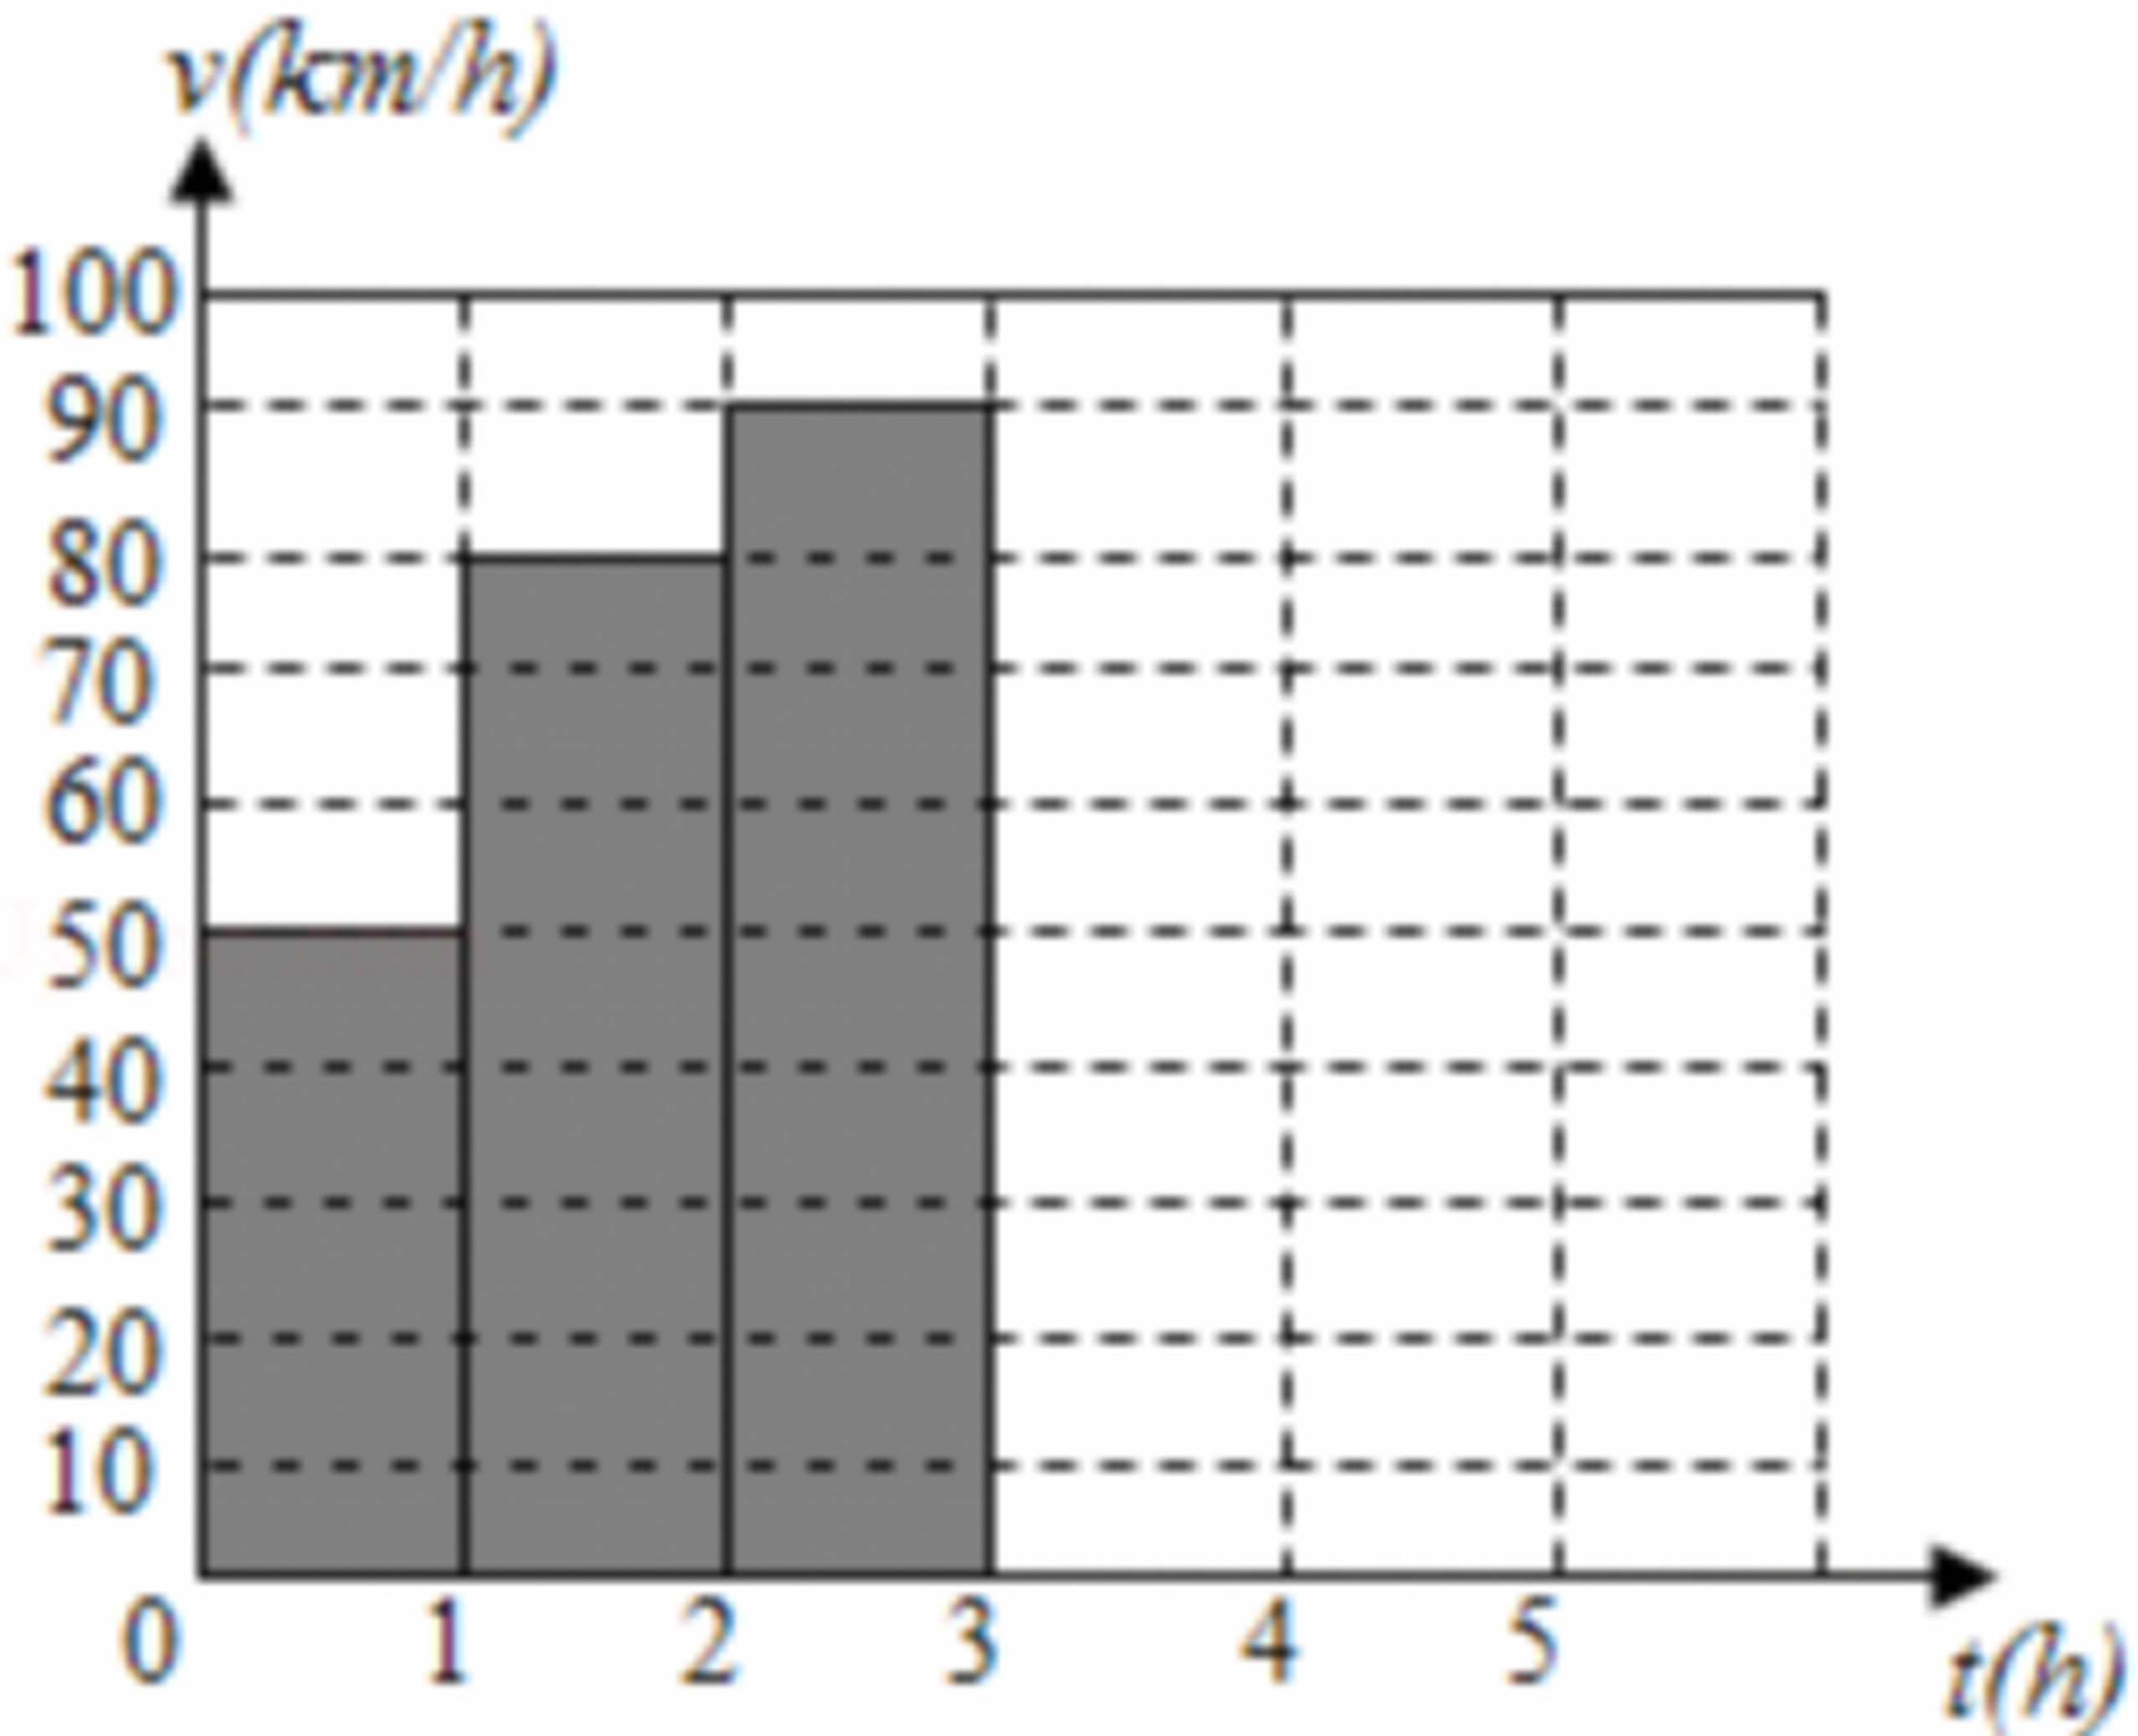
\includegraphics[width=0.52\textwidth]{figures/speed_time_bars.png}
\end{center}

\begin{enumerate}[label=(\arabic*)]
\item 求图中阴影部分的面积，并说明所求面积的实际意义；
\item 假设这辆汽车的里程表在汽车行驶这段路程前的读数为 $2004\,\mathrm{km}$，
试将汽车行驶这段路程时汽车里程表读数 $S$ 表示为时间 $t$ 的函数，
并求出当汽车里程表读数为 $2094\,\mathrm{km}$ 时，汽车行驶了多少时间？
\end{enumerate}

\ifanswer
\solbegin
\stepm{(1)}{由一辆汽车在某段路程中的行驶速度与时间的关系图，}
\step{得阴影部分的面积为 $50\times1+80\times1+90\times1=220$，}
\step{阴影部分的面积表示汽车在 $3$ 小时内行驶的路程为 $220\,\mathrm{km}$.}
\stepm{(2)}{$S=\begin{cases}
50t+2004,&0\leqslant t<1\\
80(t-1)+2054,&1\leqslant t<2\\
90(t-2)+2134,&2\leqslant t\leqslant3
\end{cases}$}
\step{令 $80(t-1)+2054=2094$，解得 $t=1.5$，所以汽车行驶 $1.5$ 小时.}
\solend

\fi

\ansspace[6]

\item 已知集合 $A=\{x\mid x<-2\text{ 或 }x\geqslant3\}$，$U=\R$.

\begin{enumerate}[label=(\arabic*)]
\item 求 $\overline{A}$；
\item 若 $B=\{x\mid mx-1>0\}$，当 $B\sub A$ 时，求实数 $m$ 的取值范围；
\item 若 $B=\{x\mid2m-6\leqslant x\leqslant m+4\}$，当 $B\cap\overline{A}=\varnothing$ 时，
求实数 $m$ 的取值范围.
\end{enumerate}

\ifanswer
\solbegin
\stepm{(1)}{因为集合 $A=\{x\mid x<-2\text{ 或 }x\geqslant3\}$，$U=\R$，
所以 $\overline{A}=\{x\mid-2\leqslant x<3\}$；}
\stepm{(2)}{当 $m=0$ 时，$B=\varnothing$，符合题意，}
\step{当 $m>0$ 时，$B=\left\{x\mid x>\dfrac1m\right\}$，则 $\dfrac1m\geqslant3$，
解得 $0<m\leqslant\dfrac13$，}
\step{当 $m<0$ 时，$B=\left\{x\mid x<\dfrac1m\right\}$，则 $\dfrac1m\leqslant-2$，
解得 $-\dfrac12\leqslant m<0$，}
\step{综上所述，实数 $m$ 的取值范围 $\left[-\dfrac12,\dfrac13\right]$；}
\stepm{(3)}{由题意得 $B=\{x\mid2m-6\leqslant x\leqslant m+4\}$，
$\overline{A}=\{x\mid-2\leqslant x<3\}$，且 $B\cap\overline{A}=\varnothing$，}
\step{当 $B=\varnothing$ 时，$2m-6>m+4$，解得 $m>10$，}
\step{当 $B\neq\varnothing$ 时，则 $\begin{cases}2m-6\leqslant m+4\\ m+4<-2\end{cases}$
或 $\begin{cases}2m-6\leqslant m+4\\ 2m-6\geqslant3\end{cases}$，}
\step{解得 $m<-6$ 或 $\dfrac92\leqslant m\leqslant10$，}
\step{综上所述，实数 $m$ 的取值范围为
$(-\infty,-6)\cup\left[\dfrac92,+\infty\right)$.}
\solend

\fi

\ansspace[8]

\item 在等腰梯形 $ABCD$ 中，$AB=DC=5$，$AD=4$，$BC=10$. 点 $E$ 在下底边 $BC$ 上.
点 $F$ 在腰 $AB$ 上.

\begin{center}
% 图取原卷截图、4× LANCZOS 放大（等腰梯形 $ABCD$ 与线段 $FE$，无辅助线）。
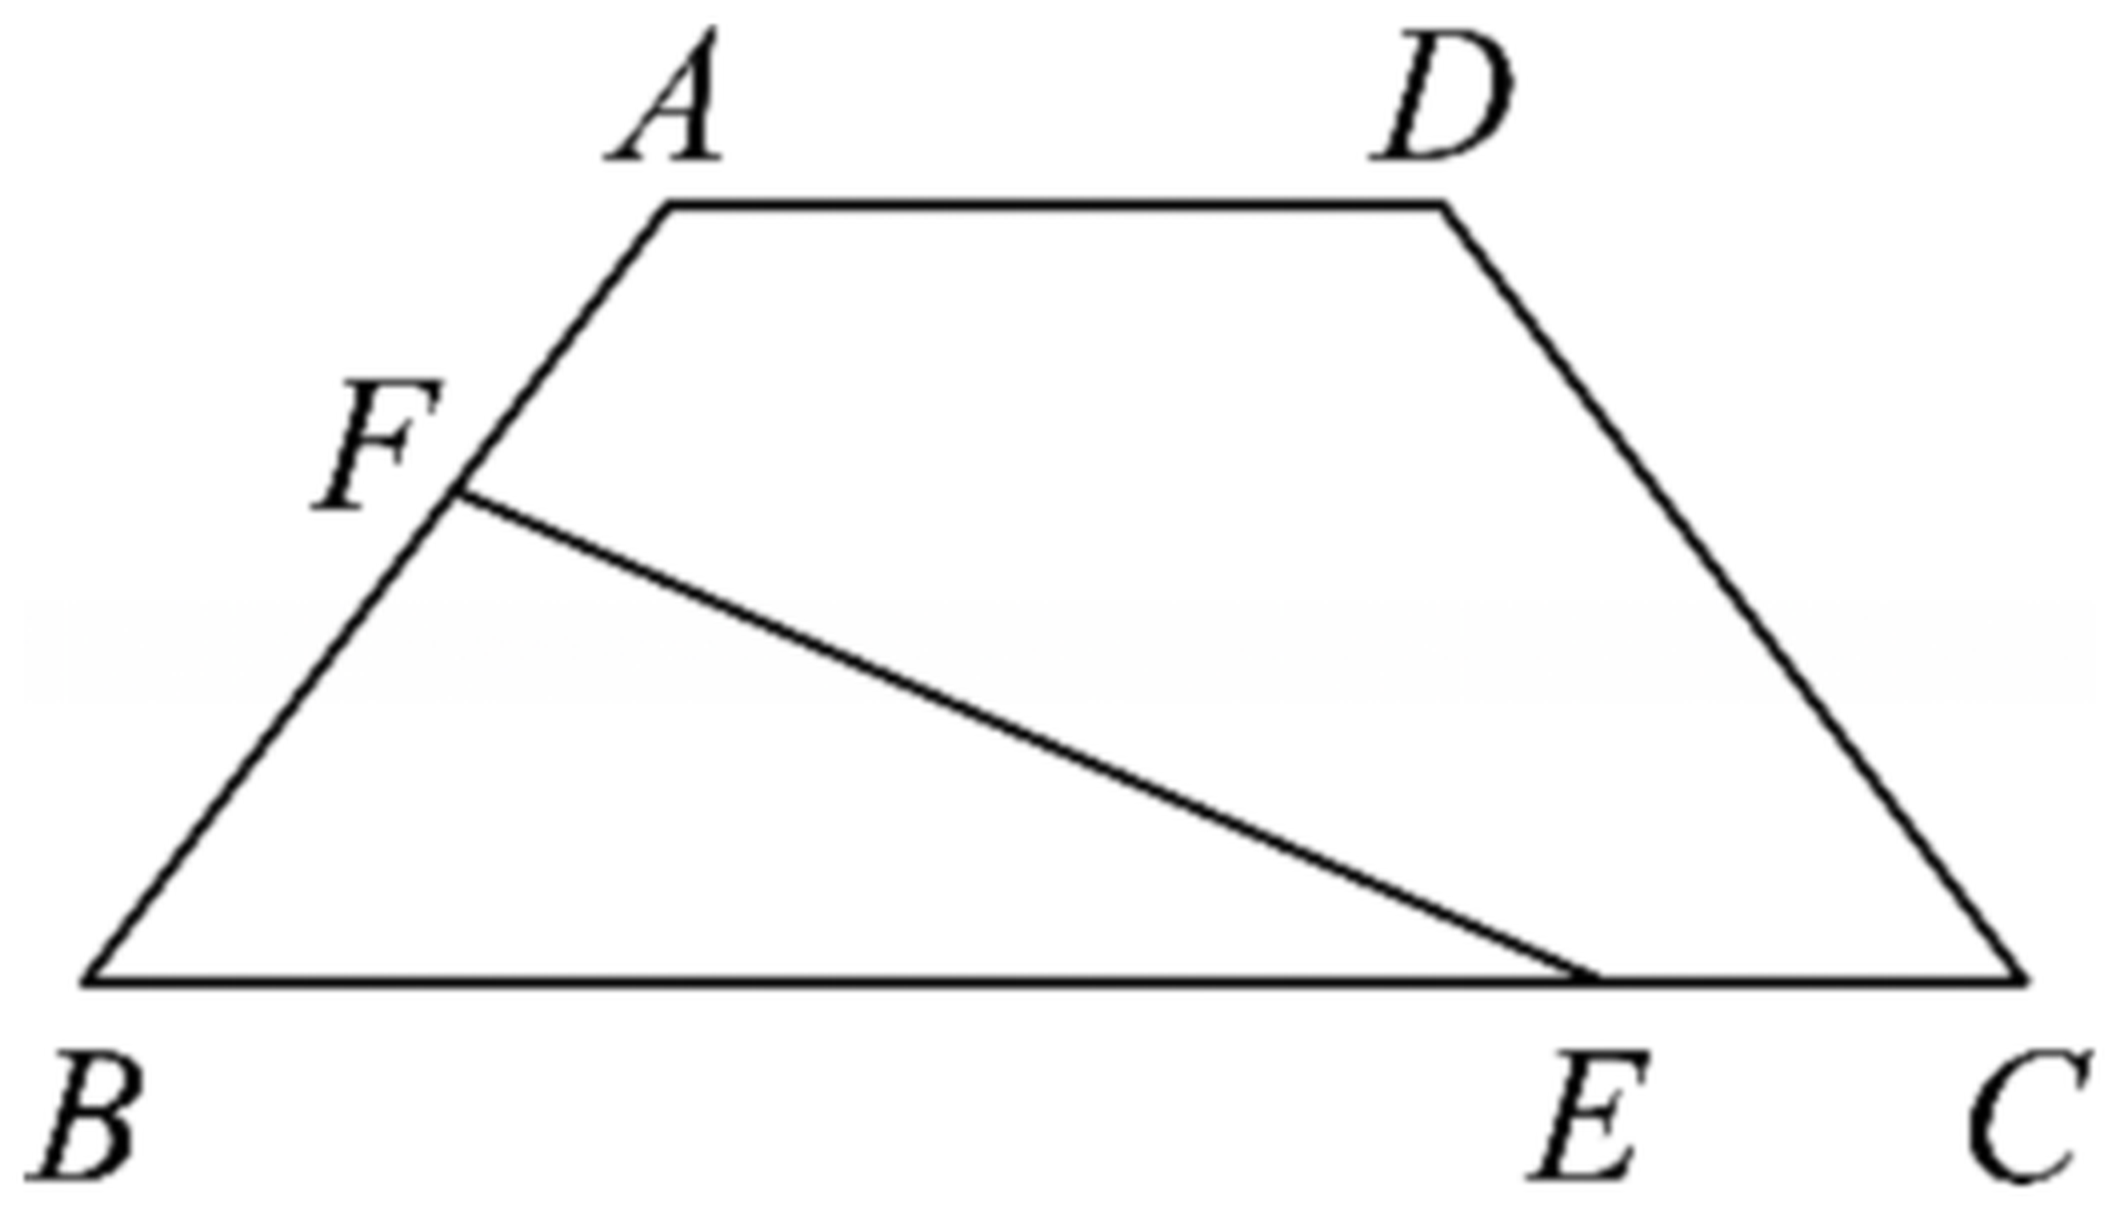
\includegraphics[width=0.46\textwidth]{figures/trapezoid_EF.png}
\end{center}

\begin{enumerate}[label=(\arabic*)]
\item 若 $EF$ 平分等腰梯形 $ABCD$ 的周长，设 $BE$ 长为 $x$，试用含 $x$ 的代数式表示
$\triangle BEF$ 的面积；
\item 是否存在线段 $EF$ 将等腰梯形 $ABCD$ 的周长和面积同时平分？若存在，求出此时 $BE$
的长；若不存在，请说明理由；
\item 是否存在线段 $EF$ 将等腰梯形 $ABCD$ 的周长和面积同时分成 $1:2$ 的两部分？
若存在，求此时 $BE$ 的长；若不存在，请说明理由.
\end{enumerate}

\ifanswer
\solbegin
\stepm{(1)}{过 $A$ 作 $AK\perp BC$ 交 $BC$ 于点 $K$，过 $F$ 作 $FG\perp BC$ 交 $BC$ 于点
$G$，}

\begin{center}
% 图取原卷截图、4× LANCZOS 放大（同梯形，多出虚线 $FG\perp BC$ 与 $AK\perp BC$
% 及两处直角符号；图只在【解析】里出现，故放进 \ifanswer 块）。
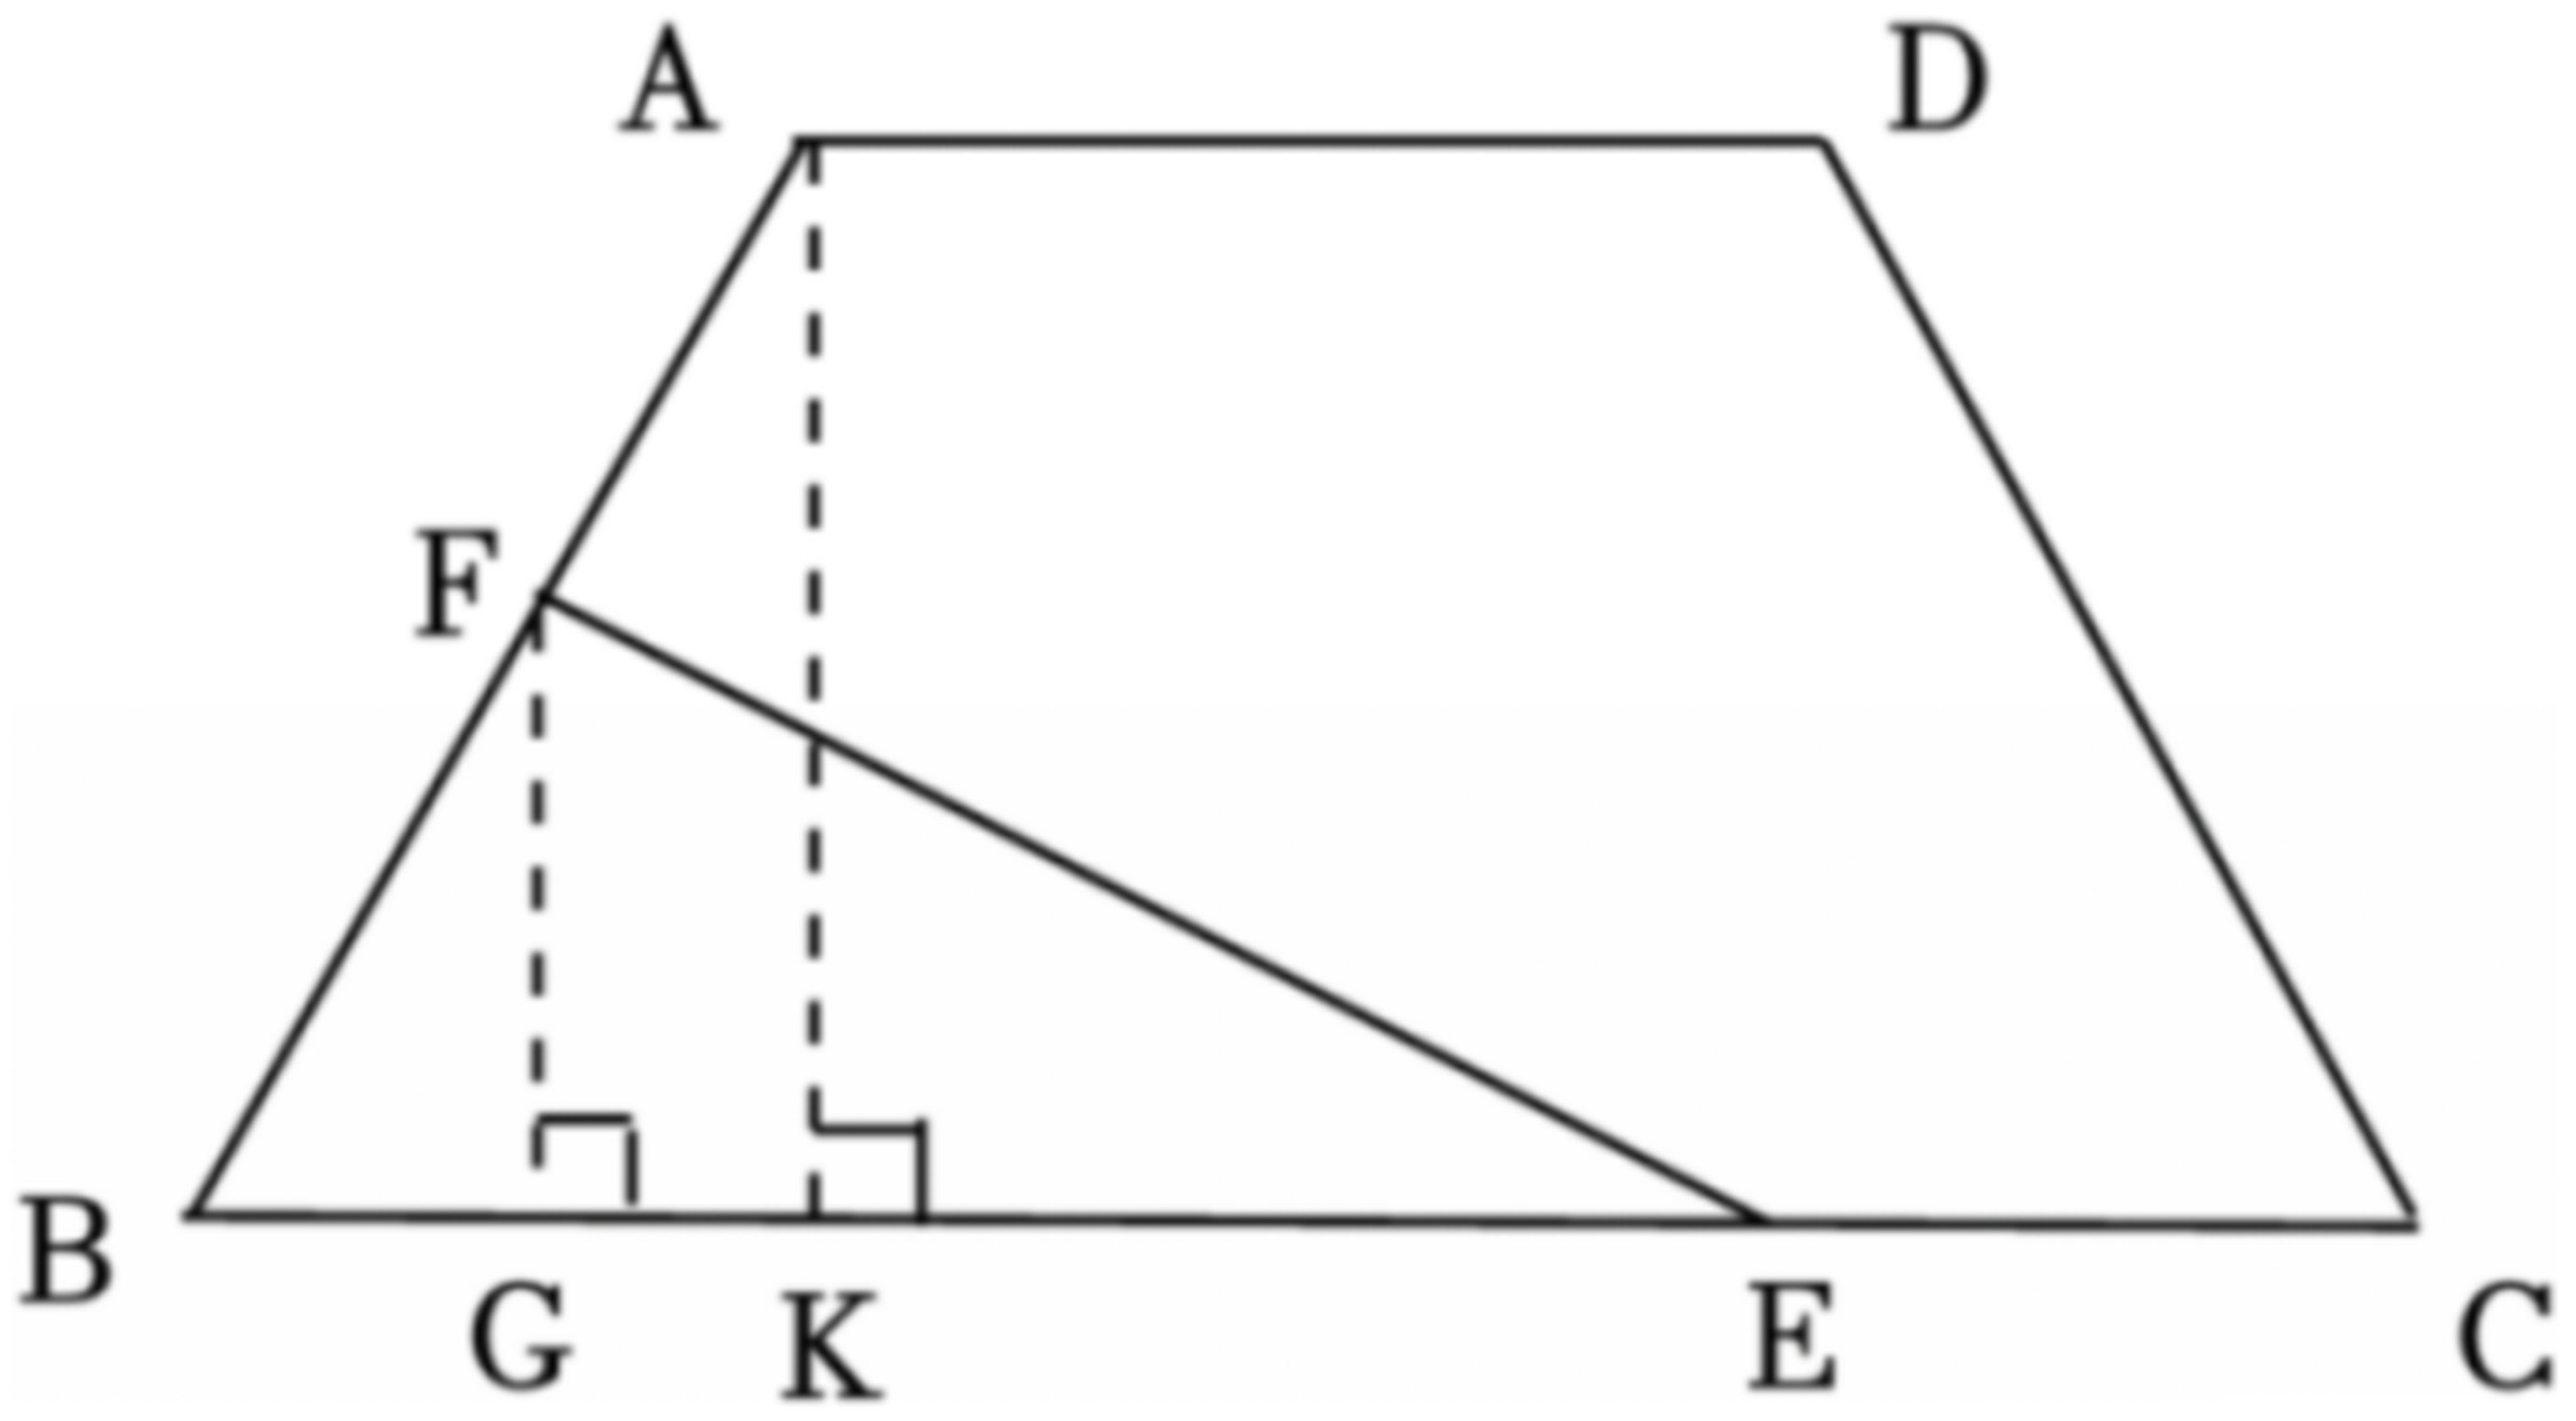
\includegraphics[width=0.62\textwidth]{figures/trapezoid_EF_aux.png}
\end{center}

\step{所以 $BK=\dfrac12\times(BC-AD)=\dfrac12\times(10-4)=3$，}
\step{$AK=\sqrt{AB^2-BK^2}=\sqrt{5^2-3^2}=4$，}
\step{由题意得，梯形 $ABCD$ 周长为 $24$，高为 $4$，面积为 $28$，}
\step{因为 $EF$ 平分等腰梯形 $ABCD$ 的周长，设 $BE$ 长为 $x$，则 $BF=12-x$，}
\step{由 $\begin{cases}0\leqslant12-x\leqslant5\\ 0\leqslant x\leqslant10\end{cases}$，
解得 $7\leqslant x\leqslant10$，}
\step{由题意得 $\triangle BFG\backsim\triangle BAK$，所以 $\dfrac{FG}{AK}=\dfrac{BF}{BA}$，
即 $\dfrac{FG}4=\dfrac{12-x}5$，}
\step{解得 $FG=\dfrac45(12-x)$，}
\step{所以 $S_{\triangle BEF}=\dfrac12BE\cdot FG
=-\dfrac25x^2+\dfrac{24}5x$（$7\leqslant x\leqslant10$）；}
\stepm{(2)}{存在，由 (1) 得 $-\dfrac25x^2+\dfrac{24}5x=\dfrac{28}2$，$x\in[7,10]$，}
\step{即 $x^2-12x+35=0$，解得 $x=7$ 或 $x=5$（舍去），}
\step{所以存在线段 $EF$ 将等腰梯形 $ABCD$ 的周长和面积同时平分，此时 $BE=7$；}
\stepm{(3)}{不存在，}
\step{情况一：$\triangle BEF$ 的面积$:$多边形 $AFECD$ 的面积 $=1:2$，
$(BE+BF):(AF+AD+DC+CE)=1:2$，}
\step{梯形周长的 $\dfrac13$ 是 $\dfrac{24}3=8$，面积的 $\dfrac13$ 是 $\dfrac{28}3$，}
\step{又因为 $BE=x$，所以 $BF=8-x$，}
\step{又因为 $\dfrac{FG}{AK}=\dfrac{BF}{BA}$，即 $\dfrac{FG}4=\dfrac{8-x}5$，
所以 $FG=\dfrac{32-4x}5$，}
\step{所以 $S_{\triangle BEF}=\dfrac12BE\times FG=-\dfrac25x^2+\dfrac{16}5x$，
所以 $\dfrac{28}3=-\dfrac25x^2+\dfrac{16}5x$，}
\step{整理得 $-3x^2+24x-70=0$，此时 $\Delta<0$，无解，故不存在；}
\step{情况二：$\triangle BEF$ 的面积$:$多边形 $AFECD$ 的面积 $=2:1$，
$(BE+BF):(AF+AD+DC+CE)=2:1$，}
\step{梯形周长的 $\dfrac13$ 为 $\dfrac{24}3=8$，面积的 $\dfrac13$ 为 $\dfrac{28}3$，
又 $BE=x$，所以 $BF=16-x$，}
\step{又 $\dfrac{FG}{AK}=\dfrac{BF}{BA}$，即 $\dfrac{FG}4=\dfrac{16-x}5$，
所以 $FG=\dfrac{64-4x}5$，}
\step{所以 $S_{\triangle BEF}=\dfrac12BE\times FG=-\dfrac25x^2+\dfrac{32}5x$，}
\step{所以 $\dfrac{28}3\times2=-\dfrac25x^2+\dfrac{32}5x$，
整理得 $-3x^2+48x-140=0$，}
\step{解得 $x=\dfrac{48+\sqrt{624}}6>10$，$x=\dfrac{48-\sqrt{624}}6<7$，
不符合题意，舍去，故不存在；}
\step{综上所述，不存在线段 $EF$ 将等腰梯形 $ABCD$ 的周长和面积同时分成 $1:2$ 的两部分.}
\solend

\fi

\ansspace[8]

\item 对集合 $\{1,2,\cdots,n\}$ 及其每一个非空子集 $A$，定义一个唯一确定的“交替和”
如下：将 $A$ 中的元素按照递减的次序排列，然后将第一个元素交替地减或加后继的元素所得的
结果，例如，子集 $\{1,2,4,6,9\}$ 的“交替和”是 $9-6+4-2+1=6$，子集 $\{5,6\}$ 的
“交替和”是 $6-5=1$，子集 $\{2\}$ 的交替和是 $2$；定义一个唯一确定的“交替积”如下：
将 $A$ 中的元素按照递减的次序排列，然后将第一个元素交替地除以或乘以后继的数所得的结果，
例如，集合 $\{1,2,4,6,9\}$ 的“交替积”是 $9\div6\times4\div2\times1=3$，
$\{5,6\}$ 的“交替积”是 $6\div5=1.2$，$\{2\}$ 的“交替积”是 $2$.

\begin{enumerate}[label=(\arabic*)]
\item 对于 $\{1,2,3,4,5,6,7,8,9\}$，求其所有子集的“交替和”的总和；
\item 对于 $\{1,2,\cdots,n\}$，求其所有子集的“交替和”的总和；
\item 对于 $\left\{n\mid\dfrac{495}{n+2}\in\N,n\in\Z\right\}$ 求其所有子集的
“交替积”的总和.
\end{enumerate}

\ifanswer
\solbegin
\stepm{(1)}{集合 $\{1,2,3,4,5,6,7,8,9\}$ 的子集中，除去 $\{9\}$ 外还有 $2^9-2$ 个
非空子集，}
\step{把这 $2^9-2$ 个非空子集两两组合后分别计算每一组中“交替和”之和，}
\step{组合原则是设 $A_i=\{9,a_1,a_2,\cdots\}$，$A_i^1=\{a_1,a_2,\cdots\}$，}
\step{集合 $A_i^1$ 的元素为集合 $A_i$ 中去掉 $9$ 的所有元素，把 $A_i$ 和 $A_i^1$
结合为一组，}
\step{显然，每组的“交替和”的和为 $9$，共有 $\dfrac{2^9-2}2$ 组，}
\step{所以，所有“交替和”之和应该为 $\dfrac{9(2^9-2)}2+9=2304$；}
\stepm{(2)}{集合 $\{1,2,\cdots,n\}$ 的子集中，除去 $\{n\}$ 外还有 $2^n-2$ 个非空子集，}
\step{把这 $2^n-2$ 个非空子集两两组合后分别计算每一组中“交替和”之和，}
\step{组合原则是设 $A_i=\{n,a_1,a_2,\cdots\}$，$A_i^1=\{a_1,a_2,\cdots\}$，}
\step{集合 $A_i^1$ 的元素为集合 $A_i$ 中去掉 $n$ 的所有元素，把 $A_i$ 和 $A_i^1$
结合为一组，}
\step{显然，每组的“交替和”的和为 $n$，共有 $\dfrac{2^n-2}2$ 组，}
% 注：下一行分子原卷印作花括号（其余同类处皆用圆括号），照抄未改，见文件头“原卷存疑”③。
\step{所以，所有“交替和”之和应该为 $\dfrac{n\{2^n-2\}}2+n=n\cdot2^{n-1}$；}
\stepm{(3)}{集合 $\left\{n\mid\dfrac{495}{n+2}\in\N,n\in\Z\right\}
=\{493,163,97,53,43,31,13,9,7,3,1,-1\}$，}
\step{其中除去 $\{-1\}$ 外还有 $2^{12}-2$ 个非空子集，}
% 注：下一行原卷把“把这”重复印了一次（“把这把这”），照抄未改，见文件头“原卷存疑”②。
\step{把这把这 $2^{12}-2$ 个非空子集两两组合后分别计算每一组中“交替积”之和，}
\step{组合原则是设 $A_j=\{-1,a_1,a_2,\cdots\}$，$A_j^1=\{a_1,a_2,\cdots\}$，}
\step{集合 $A_j^1$ 的元素为集合 $A_j$ 中去掉 $-1$ 的所有元素，把 $A_j$ 和 $A_j^1$
结合为一组，}
\step{显然，每组的“交替积”的和为 $0$，共有 $\dfrac{2^{12}-2}2$ 组，}
\step{所以，所有“交替积”之和应该为 $\dfrac{2^{12}-2}2\times0-1=-1$.}
\solend

\fi

\ansspace*[10]

\end{enumerate}

\end{document}
